\documentclass[12pt,a4paper]{book}

\usepackage{amsmath,amssymb,amsthm,amsfonts}
\usepackage{mathtools}
\usepackage{mathrsfs}
\usepackage{bm}
\usepackage{dsfont}

\usepackage{float}

\usepackage{placeins}
\usepackage{subfigure}

\usepackage{geometry}
\geometry{margin=2.5cm}

\usepackage[table]{xcolor} 
\usepackage{multicol,multirow}
\usepackage[numbers]{natbib}

\usepackage{graphicx}
\usepackage{subfigure}
\usepackage{array,cellspace}

%\usepackage[backend=biber, style=numeric]{biblatex}
\usepackage{hyperref}
%\hypersetup{backref,colorlinks,linktocpage=true}

\usepackage{setspace}
\linespread{1.7}



\usepackage[extrafootnotefeatures]{xepersian}
\settextfont[Scale=1.1]{XB Niloofar} % در صورت نیاز تغییر بده
\setlatintextfont{Times New Roman}
\setmathdigitfont{Yas}


\let\oldmathds\mathds\renewcommand{\mathds}[1]{{\SwitchToDefaultMathDigits\oldmathds{#1}}}


\newtheorem{theorem}{قضیه} % ساختار ساده
\newtheorem{lemma}[theorem]{لم} % شماره‌گذاری وابسته به قضیه
\newtheorem{definition}{تعریف} % محیطی مستقل با شماره‌گذاری مجزا

\definecolor{tablezebra}{gray}{0.95}
\setlength{\arrayrulewidth}{1pt}

\newcommand{\zeros}{\bm{\textrm{\lr{0}}}}
\newcommand{\ones}{\mathds{1}}


\def\arraystretch{1}
\setlength\cellspacetoplimit{8pt}
\setlength\cellspacebottomlimit{8pt}


%\bibliographystyle{ieeetr}
%\addbibresource{chapters/refs/ref6}

\begin{document}
	
	%======================
	% Title Page
	%======================
	\begin{titlepage}
		\centering
		
		\vspace*{2cm}
		
		{\Huge \textbf{ارتباطات کوانتومی،
				شبکه‌های کوانتومی و
				حسگری کوانتومی}
		}\\[0.8cm]
		
		{
			\Large \lr{Quantum Communication,
				Quantum Networks, and
				Quantum Sensing}
		}
		
		\vspace{2cm}
		
		{\large نویسنده:}\\[0.5cm]
		
		\lr{Ivan B. Djordjevic}
		
		\vfill
		
		{\large مترجم:}\\[0.5cm]
		محمد رضیئی فیجانی\\
اسماعیل اسکندری
		
		\vspace{1cm}
		
		{\large \today}
		
	\end{titlepage}
	
	%======================
	% Table of Contents
	%======================
	\twocolumnfootnotes	
	% !TeX root= ../quantum.tex


\chapter*{پیشگفتار}
\label{chap:preface}

اطلاعات کوانتومی\LTRfootnote{Quantum information} به استفاده از مفاهیم مکانیک کوانتومی برای انجام پردازش اطلاعات\LTRfootnote{Information processing} و انتقال اطلاعات\LTRfootnote{Information transmission} مربوط می‌شود. پردازش اطلاعات کوانتومی\LTRfootnote{Quantum information processing (QIP)} (\lr{QIP}) یک حوزه پژوهشی هیجان‌انگیز با کاربردهای متعدد است که از جمله آن‌ها می‌توان به توزیع کلید کوانتومی\LTRfootnote{Quantum key distribution (QKD)} (\lr{QKD})، دورنوردی کوانتومی\LTRfootnote{Quantum teleportation}، محاسبات کوانتومی و محاسبات کوانتومی توزیع‌شده\LTRfootnote{Distributed quantum computing}، حسگری کوانتومی\LTRfootnote{Quantum sensing}، شبکه‌بندی کوانتومی\LTRfootnote{Quantum networking}، رادار کوانتومی\LTRfootnote{Quantum radar} و یادگیری ماشین کوانتومی\LTRfootnote{Quantum machine learning} اشاره کرد. علم اطلاعات کوانتومی\LTRfootnote{Quantum information science (QIS)} (\lr{QIS})، با توجه به تعداد کتاب‌های منتشر شده در زمینه‌های \lr{QIP}، محاسبات کوانتومی و ارتباطات کوانتومی و همچنین کنفرانس‌های متعددی که صرفاً به \lr{QIS} اختصاص یافته‌اند، در حال تجربه توسعه سریعی است. با توجه به نوظهور بودن مفاهیم زیربنایی \lr{QIS}، انتظار می‌رود این موضوع مورد توجه بسیاری از دانشمندان، مهندسان، آژانس‌های دولتی، صنایع و سرمایه‌گذاران قرار گیرد، و نه فقط کسانی که در پژوهش‌های \lr{QIP} درگیر هستند. درهم‌تنیدگی\LTRfootnote{Entanglement} نشان‌دهنده یک ویژگی منحصر‌به‌فرد در \lr{QIP} است که کامپیوترهای کوانتومی را قادر می‌سازد مسائلی را حل کنند که از نظر عددی برای کامپیوترهای کلاسیک دشوار\LTRfootnote{Numerically intractable} هستند. این ویژگی همچنین حسگرهای بهبودیافته کوانتومی\LTRfootnote{Quantum-enhanced sensors} را با حساسیت‌های اندازه‌گیری\LTRfootnote{Measurement sensitivities} فراتر از محدودیت‌های کلاسیک توانمند ساخته و امنیت انتقال داده‌ی تصدیق‌پذیر\LTRfootnote{Certifiable data transmission security} را فراهم می‌کند که توسط قوانین مکانیک کوانتومی تضمین می‌شود؛ برخلاف فرضیات اثبات‌نشده‌ای که در رمزنگاری متداول\LTRfootnote{Conventional cryptography} برای امنیت محاسباتی\LTRfootnote{Computational security} استفاده می‌شوند. از درهم‌تنیدگی از پیش اشتراک‌گذاری شده\LTRfootnote{Preshared entanglement} می‌توان برای موارد زیر استفاده کرد: (۱) بهبود ظرفیت کانال کلاسیک\LTRfootnote{Classical channel capacity}، (۲) فراهم‌سازی ارتباطات امن، (۳) بهبود حساسیت حسگر، (۴) توانمندسازی محاسبات کوانتومی توزیع‌شده، (۵) فراهم‌سازی حسگری توزیع‌شده به کمک درهم‌تنیدگی\LTRfootnote{Entanglement-assisted distributed sensing}، و (۶) فراهم‌سازی دسترسی به کامپیوتر کوانتومی با امنیت اثبات‌پذیر، و همچنین انجام بسیاری از وظایف دیگر.

به دلیل ماهیت بین‌رشته‌ای \lr{QIS}، این کتاب با هدف ایجاد تعادل مناسب میان \lr{QIP}، تصحیح خطای کوانتومی\LTRfootnote{Quantum error correction}، ارتباطات کوانتومی، حسگری کوانتومی و شبکه‌بندی کوانتومی نگاشته شده است. اهداف اصلی کتاب را می‌توان به شرح زیر خلاصه کرد:

\begin{enumerate}
	\item کتاب روندها را در \lr{QIP}، تصحیح خطای کوانتومی، ارتباطات کوانتومی، حسگری کوانتومی، شبکه‌بندی کوانتومی و یادگیری ماشین کوانتومی توصیف می‌کند.
	\item کتاب یک مقدمه جامع و خودکفا\LTRfootnote{Self-contained introduction} برای ارتباطات کوانتومی، تصحیح خطای کوانتومی، حسگری کوانتومی و شبکه‌بندی کوانتومی ارائه می‌دهد.
	\item کتاب طیف گسترده‌ای از خوانندگان را هدف قرار می‌دهد: مهندسان برق، مهندسان مخابرات، مهندسان اپتیک، ریاضی‌دانان کاربردی، دانشمندان علوم کامپیوتر و فیزیک‌دانان.
	\item کتاب نیازی به دانش قبلی از مکانیک کوانتومی یا \lr{QIP} ندارد. مفاهیم پایه در فصل \ref{chap:3} ارائه شده‌اند.
	\item کتاب به هیچ پیش‌زمینه پیش‌نیازی نیاز ندارد، به‌جز درک مفاهیم پایه جبر برداری در سطح مقطع کارشناسی.
	\item برای خوانندگانی که با نظریه اطلاعات\LTRfootnote{Information theory}، کدگذاری کانال\LTRfootnote{Channel coding} و نظریه آشکارسازی\LTRfootnote{Detection theory} آشنا نیستند، فصل \ref{chap:2} مفاهیم و تعاریف پایه را در حوزه‌های مربوطه ارائه می‌دهد. این فصل تنها مفاهیم نظریه اطلاعات، کدگذاری و آشکارسازی را پوشش می‌دهد که در فصل‌های بعدی مرتبط هستند.
	\item خوانندگانی که به تصحیح خطای کوانتومی علاقه‌مند نیستند، همچنان می‌توانند از دیگر فصل‌های کتاب استفاده کنند.
	\item خوانندگانی که صرفاً به تصحیح خطای کوانتومی علاقه‌مند هستند، نیازی به مطالعه سایر فصل‌ها به‌جز فصل‌های \ref{chap:3} و \ref{chap:4} ندارند و می‌توانند تنها بر فصل‌های تصحیح خطای کوانتومی تمرکز کنند. در واقع، تلاشی صورت گرفته تا فصل‌ها مستقل باشند و در عین حال جریان مناسبی بین آن‌ها برقرار باشد.
	\item کتاب با مفاهیم شهودی\LTRfootnote{Intuitive concepts} و پایه شروع شده و سپس به سمت موضوعات با دشواری متوسط و در نهایت به موضوعات پیچیده و درگیر با ریاضیات حرکت می‌کند.
	\item چندین درس را می‌توان با استفاده از این کتاب ارائه داد. مثال‌ها شامل دروسی در زمینه‌های زیر است: (۱) تصحیح خطای کوانتومی، (۲) \lr{QIP} و یادگیری ماشین کوانتومی، (۳) ارتباطات کوانتومی، (۴) حسگری کوانتومی، (۵) شبکه‌بندی کوانتومی، و (۶) یکپارچه‌سازی\LTRfootnote{Integration} مفاهیم ارتباطات کوانتومی، حسگری کوانتومی و شبکه‌بندی کوانتومی.
	\item خواننده‌ای که این کتاب را به پایان برساند، قادر خواهد بود در زمینه‌های مختلف \lr{QIS} به پژوهش مستقل بپردازد.
\end{enumerate}

این کتاب یک مقدمه خودکفا برای اطلاعات کوانتومی، ارتباطات کوانتومی، تصحیح خطای کوانتومی، حسگری کوانتومی و شبکه‌بندی کوانتومی است. خواننده موفق کتاب برای مطالعه بیشتر در این حوزه‌ها آماده خواهد بود و برای انجام پژوهش مستقل مهیا می‌شود. خواننده‌ای که کتاب را به پایان رسانده باشد، قادر به طراحی مدارات \lr{QIP}، کدهای پایدارساز\LTRfootnote{Stabilizer codes}، کدهای \lr{CSS}\LTRfootnote{Calderbank-Shor-Steane (CSS) codes}، کدهای زیرسیستم\LTRfootnote{Subsystem codes}، کدهای توپولوژیکی\LTRfootnote{Topological codes}، کدهای سطحی\LTRfootnote{Surface codes} و کدهای تصحیح خطای کوانتومی به کمک درهم‌تنیدگی\LTRfootnote{Entanglement-assisted quantum error correction codes} خواهد بود. همچنین، خواننده در زمینه تصحیح خطای کوانتومی تحمل‌پذیر خطا\LTRfootnote{Fault-tolerant} مهارت خواهد یافت. علاوه بر این، خواننده در ارتباطات کوانتومی، \lr{QKD} و یادگیری ماشین کوانتومی مسلط خواهد شد و دانش لازم در حسگری کوانتومی و رادارهای کوانتومی را برای انجام پژوهش مستقل در این زمینه‌ها کسب خواهد کرد. خوانندگان این کتاب همچنین قادر خواهند بود فرستنده-گیرنده‌های کوانتومی\LTRfootnote{Quantum transceivers} مناسب برای کاربردهای ارتباطات کوانتومی و حسگری کوانتومی را پیشنهاد دهند. علاوه بر این، خوانندگان کتاب قادر به پیشنهاد پروتکل‌های شبکه‌بندی ارتباطات کوانتومی و معماری‌های شبکه‌بندی کوانتومی خواهند بود.

برخی از ویژگی‌های منحصر‌به‌فرد کتاب را می‌توان به شرح زیر خلاصه کرد:
\begin{enumerate}
	\item این کتاب حوزه‌های \lr{QIP}، ارتباطات، تصحیح خطا، حسگری، شبکه‌بندی و یادگیری ماشین را یکپارچه می‌کند.
	\item کتاب نیازی به دانش مکانیک کوانتومی ندارد.
	\item این کتاب به هیچ مطلب پیش‌نیازی به‌جز مفاهیم پایه جبر برداری در سطح کارشناسی نیاز ندارد.
	\item این کتاب شرح عمیقی از طراحی مدارها و ماژول‌های \lr{QIP}، تصحیح خطا، ارتباطات و شبکه‌بندی، و حسگری ارائه می‌دهد.
	\item دانشجوی موفق برای مطالعه بیشتر در این زمینه‌ها آماده شده و واجد شرایط انجام پژوهش مستقل خواهد بود.
	\item خواننده‌ای که این کتاب را به پایان رسانده باشد، قادر به طراحی مدارات پردازش اطلاعات، کدهای پایدارساز، کدهای \lr{CSS}، کدهای توپولوژیکی، کدهای سطحی، کدهای زیرسیستم، کدهای بررسی توازن کم‌چگال (\lr{LDPC}) کوانتومی\LTRfootnote{Quantum low-density parity-check (LDPC) codes} و کدهای تصحیح خطای کوانتومی به کمک درهم‌تنیدگی خواهد بود و در طراحی تحمل‌پذیر خطا مهارت خواهد یافت.
	\item دانشجوی موفق قادر خواهد بود فرستنده-گیرنده‌های کوانتومی را برای کاربردهای ارتباطات کوانتومی و حسگری کوانتومی پیشنهاد دهد.
	\item دانشجوی موفق قادر به پیشنهاد پروتکل‌های شبکه‌بندی ارتباطات کوانتومی و معماری‌های شبکه‌بندی کوانتومی خواهد بود.
	\item دانشجویانی که کتاب را به پایان رسانده باشند، در یادگیری ماشین کوانتومی مهارت خواهند یافت.
	\item در نهایت، دانشجویان در \lr{QKD} و دورنوردی کوانتومی مسلط خواهند شد.
	\item مطالب اضافی برای پشتیبانی از کتاب در یک وب‌سایت همراه که پس از انتشار توسعه می‌یابد، ارائه خواهد شد.
\end{enumerate}

نویسنده مایل است از حمایت بنیاد ملی علوم (\lr{NSF}) قدردانی نماید. در نهایت، تشکر ویژه‌ای از \lr{Prem Kumar Kaliamoorthi}، \lr{Kyle Gravel} و \lr{Tim Pitts} از انتشارات الزویر به‌خاطر تلاش‌های بی‌وقفه‌شان در سازماندهی امور لجستیکی کتاب، از جمله ویرایش و ترویج، که برای به ثمر رسیدن این کتاب ضروری بودند، به‌عمل می‌آید.










		
	\tableofcontents
	\newpage
	
	

	\chapter{مقدمه}
\label{chap:1}


\section*{چکیده}

در این فصل، مفاهیم پایه هر دو حوزه امنیت لایه فیزیکی\LTRfootnote{Physical-layer security (PLS)} (\lr{PLS}) و توزیع کلید کوانتومی\LTRfootnote{Quantum key distribution (QKD)} (\lr{QKD}) معرفی می‌شوند. فصل با بررسی نقش \lr{PLS} آغاز شده و با مروری کوتاه بر سیستم‌های رمزنگاری متداول مبتنی بر کلید ادامه می‌یابد. سپس مفهوم امنیت نظریه-اطلاعاتی\LTRfootnote{Information-theoretic security} معرفی شده و شرط محرمانگی کامل\LTRfootnote{Perfect secrecy condition} تشریح می‌گردد. امنیت محاسباتی\LTRfootnote{Computational security} به‌عنوان مورد خاصی از امنیت نظریه-اطلاعاتی توصیف می‌شود که در آن چندین مورد تعدیل\LTRfootnote{Relaxation} معرفی شده است. در ادامه، مفاهیم محرمانگی قوی و ضعیف ارائه می‌شوند. علاوه بر این، مدل کانال شنود تخریب‌شده\LTRfootnote{Degraded wiretap channel} که توسط واینر\LTRfootnote{Wyner} معرفی شده، توصیف گردیده و کدهای کانال شنود متناظر تعریف می‌شوند. سپس، کانال پخش با پیام‌های محرمانه\LTRfootnote{Broadcast channel with confidential messages} که توسط سیزار\LTRfootnote{Csiszár} و کورنر\LTRfootnote{Körner} معرفی شده است، به همراه کد تصادفی\LTRfootnote{Stochastic code} مربوطه شرح داده می‌شود. آخرین موضوع در بخش \lr{PLS} به پروتکل توافق کلید مخفی اختصاص یافته است. بخش \lr{QKD} ابتدا نحوه شکستن پروتکل \lr{RSA} را به کمک الگوریتم تجزیه شور\LTRfootnote{Shor’s factorization algorithm} توصیف کرده و در ادامه توصیف کوتاهی از مبانی طرح‌های \lr{QKD} با متغیر گسسته\LTRfootnote{Discrete variable (DV)} (\lr{DV}) و متغیر پیوسته\LTRfootnote{Continuous variable (CV)} (\lr{CV}) ارائه می‌دهد. محدودیت‌های کلیدی طرح‌های \lr{DV-QKD} شناسایی شده و پروتکل‌های مختلف \lr{QKD} در سه دسته کلی قرار می‌گیرند: \lr{QKD} وابسته به دستگاه، \lr{QKD} مستقل از دستگاه منبع و \lr{QKD} مستقل از دستگاه اندازه‌گیری\LTRfootnote{Measurement device-independent (MDI)} (\lr{MDI}). علاوه بر این، تعریف کسر محرمانگی\LTRfootnote{Secrecy fraction} برای پروتکل‌های \lr{QKD} ارائه شده و به‌دنبال آن شرح کوتاهی از حملات انفرادی (غیرهمدوس) و دسته‌جمعی، و توضیحی درباره نحوه محاسبه کسر محرمانگی متناظر آورده شده است. در بخش سازمان‌دهی کتاب، توصیف دقیقی از محتوای فصل‌ها ارائه می‌گردد.

\section{مبانی امنیت لایه فیزیکی}
\label{sec:1-1}
رمزنگاری کلید عمومی دارای چندین نقص جدی است، از جمله: پیاده‌سازی آن در دستگاه‌هایی با محدودیت حافظه و پردازش پایین دشوار است، اینترنت به‌طور فزاینده‌ای در حال متحرک شدن است، طرح‌های امنیتی بر پایه فرضیات اثبات‌نشده‌ای از دشواری\LTRfootnote{Intractability} توابع خاص بنا شده‌اند، و فرضِ محدود بودن منابع محاسباتی ایو\LTRfootnote{Eve} در بسیاری از موارد نادرست است. مدل مرجع اتصال متقابل سیستم‌های باز\LTRfootnote{Open system interconnection (OSI)} (\lr{OSI}) هفت لایه را تعریف می‌کند. با این حال، در شکل \ref{fig:1-1} تنها پنج لایه مرتبط با مسائل امنیتی ارائه شده است. مدل اصلی \lr{OSI} حتی مسائل امنیتی را به‌هیچ‌وجه مشخص نمی‌کند. مسائل امنیتی در استاندارد \lr{X.800} (معماری امنیتی برای \lr{OSI}) مورد توجه قرار گرفته‌اند \cite{1-1}. با این حال، نه امنیت لایه فیزیکی (\lr{PLS}) \cite{1-2, 1-3, 1-4, 1-5, 1-6} و نه توزیع کلید کوانتومی (\lr{QKD}) \cite{1-7, 1-8, 1-9, 1-10, 1-11} در این استاندارد مورد بحث قرار نگرفته‌اند. با این وجود، سرویس‌های مشخص‌شده در این پنج لایه را می‌توان با به‌کارگیری \lr{PLS} و \lr{QKD} به‌طور قابل‌توجهی بهبود بخشید. طرح‌های \lr{PLS} و \lr{QKD} می‌توانند به‌صورت مستقل نیز عمل کنند.

\begin{figure}[ht]
	\centering
	 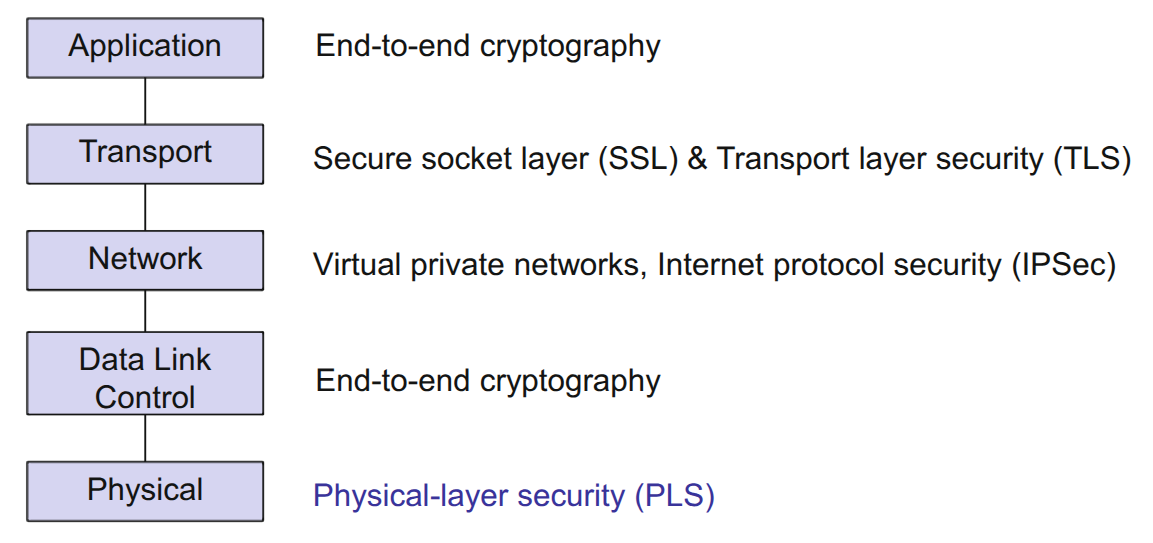
\includegraphics[width=0.8\textwidth]{chapters/figs/fig-1-1}
	\caption{مکانیزم‌های امنیتی در لایه‌های مختلف مدل \lr{OSI}. تنها لایه‌های مرتبط با امنیت نشان داده شده‌اند.}
	\label{fig:1-1}
\end{figure}

\begin{figure}[ht]
	\centering
	 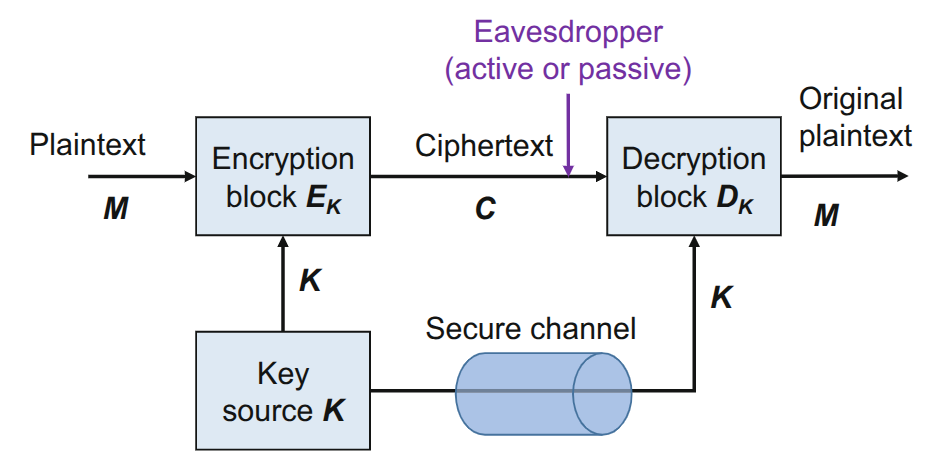
\includegraphics[width=0.8\textwidth]{chapters/figs/fig-1-2}
	\caption{طرح رمزنگاری پایه مبتنی بر کلید.}
	\label{fig:1-2}
\end{figure}

\begin{figure}[ht]
	\centering
	 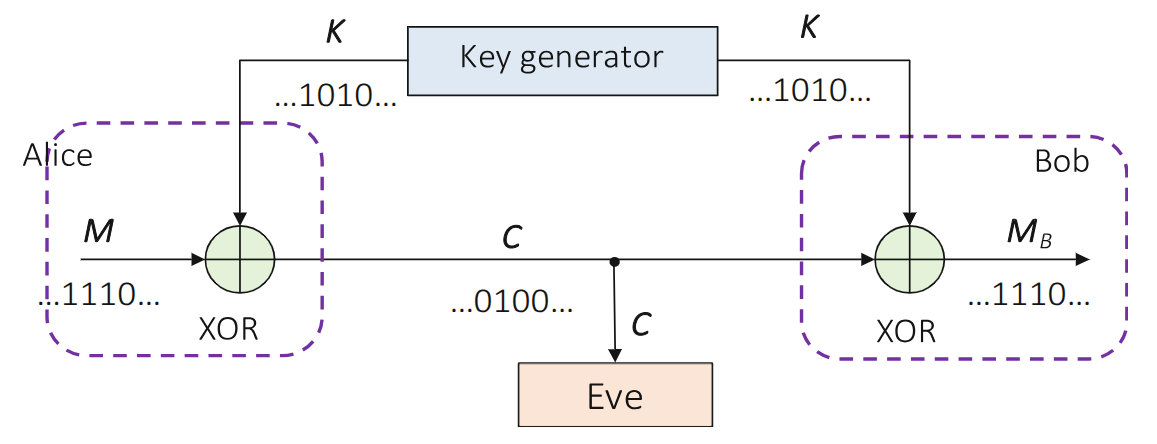
\includegraphics[width=0.8\textwidth]{chapters/figs/fig-1-3}
	\caption{طرح رمزگذاری پد یک‌بار مصرف.}
	\label{fig:1-3}
\end{figure}

سیستم رمزنگاری پایه مبتنی بر کلید \cite{1-12, 1-13, 1-14, 1-15, 1-16, 1-17, 1-18, 1-19, 1-20, 1-21, 1-22} در شکل \ref{fig:1-2} ارائه شده است. منبع، پیام (متن‌آشکار\LTRfootnote{Plaintext}) $M$ را به سمت بلوک رمزگذاری ارسال می‌کند که این بلوک با کمک کلید $K$ دریافت شده از منبع کلید، رمزنگاشت (متن‌رمز\LTRfootnote{Ciphertext}) $C$ را تولید می‌کند. در سمت گیرنده، رمزنگاشت ارسال شده از طریق یک کانال ناامن، توسط الگوریتم رمزگشایی به همراه کلید $K$ که از طریق کانال امن دریافت شده است، پردازش می‌شود که متن‌آشکار اصلی را برای تحویل به کاربر احرازهویت‌شده بازسازی می‌کند. فرآیند رمزگذاری را می‌توان به‌صورت ریاضی به‌صورت $E_K(M) = C$ توصیف کرد، در حالی که فرآیند رمزگشایی با $D_K(C) = M$ بیان می‌شود. ترکیب توابع رمزگشایی و رمزگذاری منجر به نگاشت همانی 	$D_K(E_K(M)) = M$ می‌گردد.
منبع کلید معمولاً کلید را به‌صورت تصادفی از فضای کلید\LTRfootnote{Keyspace} (محدوده مقادیر ممکن برای کلید) تولید می‌کند.


الگوریتم‌های مبتنی بر کلید را می‌توان به دو دسته کلی تقسیم کرد:
\begin{itemize}
	\item \textbf{الگوریتم‌های متقارن\LTRfootnote{Symmetric algorithms}:} که در آن‌ها کلید رمزگشایی را می‌توان از کلید رمزگذاری مشتق کرد و بالعکس. متناوباً، می‌توان از یک کلید یکسان برای هر دو مرحله رمزگذاری و رمزگشایی استفاده کرد. الگوریتم‌های متقارن با نام‌های الگوریتم‌های تک‌کلیدی\LTRfootnote{One-key (single-key) algorithms} یا کلید‌مخفی\LTRfootnote{Secret-key algorithms} نیز شناخته می‌شوند. سیستم شناخته‌شده‌ای که از این نوع الگوریتم بهره می‌برد، استاندارد رمزگذاری دیجیتال\LTRfootnote{Digital Encryption Standard (DES)} (\lr{DES}) است \cite{1-13, 1-14, 1-15, 1-16, 1-17, 1-18}.
	\item \textbf{الگوریتم‌های نامتقارن\LTRfootnote{Asymmetric algorithms}:} که در آن‌ها کلیدهای رمزگذاری و رمزگشایی متفاوت هستند. علاوه بر این، کلید رمزگشایی را نمی‌توان در یک بازه زمانی معقول از روی کلید رمزگذاری تعیین کرد. به دلیل این واقعیت، کلیدهای رمزگذاری حتی می‌توانند به‌صورت عمومی منتشر شوند، به‌طوری که یک شنودگر\LTRfootnote{Eavesdropper} قادر به تعیین کلید رمزگشایی نخواهد بود. سیستم‌های کلید عمومی\LTRfootnote{Public-key systems} \cite{1-17} بر پایه این مفهوم بنا شده‌اند. در سیستم‌های کلید عمومی، کلیدهای رمزگذاری به‌صورت عمومی منتشر می‌شوند، در حالی که کلید رمزگشایی تنها برای کاربر موردنظر شناخته شده است. در این حالت، کلید رمزگذاری را کلید عمومی\LTRfootnote{Public key} و کلید رمزگشایی را کلید مخفی (خصوصی)\LTRfootnote{Secret (private) key} می‌نامند. این کلیدها را می‌توان با هر ترتیبی برای ایجاد رمزنگاشت از متن‌آشکار و بازسازی متن‌آشکار از رمزنگاشت به کار برد.
\end{itemize}

ساده‌ترین سیستم رمزنگاری کلید خصوصی، رمز ورنام\LTRfootnote{Vernam cipher} است که با نام پد یک‌بار مصرف\LTRfootnote{One-time pad} نیز شناخته می‌شود. در یک پد یک‌بار مصرف \cite{1-23}، یک دنباله کاملاً تصادفی از نویسه‌ها، با طولی برابر با طول دنباله پیام، به‌عنوان کلید استفاده می‌شود. زمانی که برای هر پیام جدید از یک دنباله تصادفی دیگر به‌عنوان کلید استفاده شود، طرح پد یک‌بار مصرف به‌اصطلاح \textit{امنیت کامل}\LTRfootnote{Perfect security} را فراهم می‌کند. به بیان دقیق‌تر، در رویکرد جستجوی جامع\LTRfootnote{Brute-force search}، بررسی $m^n$ کلید احتمالی لازم خواهد بود که در آن $m$ اندازه الفبای به‌کار رفته و $n$ طول رمزنگاشتِ شنود شده است. در عمل، در ارتباطات دیجیتال و کامپیوتری، ما معمولاً در الفبای باینری $\{0, 1\}$ عمل می‌کنیم. برای به‌دست آوردن کلید، به یک مولد تصادفی خاص نیاز داریم و برای رمزگذاری با استفاده از طرح پد یک‌بار مصرف، صرفاً عمل جمع در پیمانه ۲ یا همان عملیات \lr{XOR} را مطابق شکل \ref{fig:1-3} انجام می‌دهیم. اگرچه طرح پد یک‌بار مصرف امنیت کامل را ارائه می‌دهد، اما چندین نقص دارد \cite{1-9, 1-10, 1-11}: این طرح مستلزم توزیع امن کلید است، طول کلید باید حداقل به اندازه پیام باشد، بیت‌های کلید نمی‌توانند مجدداً استفاده شوند، کلیدها باید پیش از موعد تحویل داده شوند، تا زمان استفاده به‌صورت امن ذخیره گردند و پس از استفاده نابود شوند.

الگوریتم‌های مبتنی بر کلید را می‌توان به دو دسته کلی تقسیم کرد:
\begin{itemize}
	\item \textbf{الگوریتم‌های متقارن\LTRfootnote{Symmetric algorithms}:} که در آن‌ها کلید رمزگشایی را می‌توان از کلید رمزگذاری مشتق کرد و بالعکس. متناوباً، می‌توان از یک کلید یکسان برای هر دو مرحله رمزگذاری و رمزگشایی استفاده کرد. الگوریتم‌های متقارن با نام‌های الگوریتم‌های تک‌کلیدی\LTRfootnote{One-key (single-key) algorithms} یا کلید‌مخفی\LTRfootnote{Secret-key algorithms} نیز شناخته می‌شوند. سیستم شناخته‌شده‌ای که از این نوع الگوریتم بهره می‌برد، استاندارد رمزگذاری دیجیتال\LTRfootnote{Digital Encryption Standard (DES)} (\lr{DES}) است \cite{1-13, 1-14, 1-15, 1-16, 1-17, 1-18}.
	\item \textbf{الگوریتم‌های نامتقارن\LTRfootnote{Asymmetric algorithms}:} که در آن‌ها کلیدهای رمزگذاری و رمزگشایی متفاوت هستند. علاوه بر این، کلید رمزگشایی را نمی‌توان در یک بازه زمانی معقول از روی کلید رمزگذاری تعیین کرد. به دلیل این واقعیت، کلیدهای رمزگذاری حتی می‌توانند به‌صورت عمومی منتشر شوند، به‌طوری که یک شنودگر\LTRfootnote{Eavesdropper} قادر به تعیین کلید رمزگشایی نخواهد بود. سیستم‌های کلید عمومی\LTRfootnote{Public-key systems} \cite{1-17} بر پایه این مفهوم بنا شده‌اند. در سیستم‌های کلید عمومی، کلیدهای رمزگذاری به‌صورت عمومی منتشر می‌شوند، در حالی که کلید رمزگشایی تنها برای کاربر موردنظر شناخته شده است. در این حالت، کلید رمزگذاری را کلید عمومی\LTRfootnote{Public key} و کلید رمزگشایی را کلید مخفی (خصوصی)\LTRfootnote{Secret (private) key} می‌نامند. این کلیدها را می‌توان با هر ترتیبی برای ایجاد رمزنگاشت از متن‌آشکار و بازسازی متن‌آشکار از رمزنگاشت به کار برد.
\end{itemize}

ساده‌ترین سیستم رمزنگاری کلید خصوصی، رمز ورنام\LTRfootnote{Vernam cipher} است که با نام پد یک‌بار مصرف\LTRfootnote{One-time pad} نیز شناخته می‌شود. در یک پد یک‌بار مصرف \cite{1-23}، یک دنباله کاملاً تصادفی از نویسه‌ها، با طولی برابر با طول دنباله پیام، به‌عنوان کلید استفاده می‌شود. زمانی که برای هر پیام جدید از یک دنباله تصادفی دیگر به‌عنوان کلید استفاده شود، طرح پد یک‌بار مصرف به‌اصطلاح \textit{امنیت کامل}\LTRfootnote{Perfect security} را فراهم می‌کند. به بیان دقیق‌تر، در رویکرد جستجوی جامع\LTRfootnote{Brute-force search}، بررسی $m^n$ کلید احتمالی لازم خواهد بود که در آن $m$ اندازه الفبای به‌کار رفته و $n$ طول رمزنگاشتِ شنود شده است. در عمل، در ارتباطات دیجیتال و کامپیوتری، ما معمولاً در الفبای باینری $\{0, 1\}$ عمل می‌کنیم. برای به‌دست آوردن کلید، به یک مولد تصادفی خاص نیاز داریم و برای رمزگذاری با استفاده از طرح پد یک‌بار مصرف، صرفاً عمل جمع در پیمانه ۲ یا همان عملیات \lr{XOR} را مطابق شکل \ref{fig:1-3} انجام می‌دهیم. اگرچه طرح پد یک‌بار مصرف امنیت کامل را ارائه می‌دهد، اما چندین نقص دارد \cite{1-9, 1-10, 1-11}: این طرح مستلزم توزیع امن کلید است، طول کلید باید حداقل به اندازه پیام باشد، بیت‌های کلید نمی‌توانند مجدداً استفاده شوند، کلیدها باید پیش از موعد تحویل داده شوند، تا زمان استفاده به‌صورت امن ذخیره گردند و پس از استفاده نابود شوند.


طبق گفته شانون\cite{1-12}، امنیت کامل\LTRfootnote{Perfect security} که با نام امنیت غیرمشروط\LTRfootnote{Unconditional security} نیز شناخته می‌شود، زمانی حاصل می‌گردد که پیام‌ها و رمزنگاشت‌ها از نظر آماری مستقل باشند، به‌طوری که اطلاعات متقابل\LTRfootnote{Mutual information} متناظر بین پیام $\bm{M}$ و رمزنگاشت $\bm{C}$ برابر با صفر شود:
\begin{equation}
	I(\bm{M}; \bm{C}) = H(\bm{M}) - H(\bm{M}|\bm{C}) = 0 \implies H(\bm{M}|\bm{C}) = H(\bm{M}),
\end{equation}
که در آن $H(\bm{M})$ آنتروپی\LTRfootnote{Entropy} (عدم قطعیت\LTRfootnote{Uncertainty}) درباره پیام و $H(\bm{M}|\bm{C})$ آنتروپی شرطی\LTRfootnote{Conditional entropy} پیام $\bm{M}$ به شرط رمزنگاشت $\bm{C}$ است. بنابراین، شرط محرمانگی کامل را می‌توان به‌صورت زیر خلاصه کرد:
\begin{equation}
	H(\bm{M}) \leq H(\bm{K}).
	\label{eq:1-2}
\end{equation}
به عبارت دیگر، برای اینکه یک طرح رمزگذاری از امنیت کامل برخوردار باشد، آنتروپی (عدم قطعیت) کلید نمی‌تواند کمتر از آنتروپی پیام باشد. با توجه به اینکه در رمز ورنام طول کلید حداقل برابر با طول پیام است، به نظر می‌رسد طرح پد یک‌بار مصرف دارای امنیت کامل باشد.

با این حال، از آنجایی که برآورده کردن این شرط دشوار است، در رمزنگاری متداول به جای امنیت نظریه-اطلاعاتی\LTRfootnote{Information-theoretic security}، از امنیت محاسباتی\LTRfootnote{Computational security} استفاده می‌شود \cite{1-10, 1-13, 1-16, 1-22, 1-23, 1-24, 1-25}. امنیت محاسباتی دو مورد تعدیل\LTRfootnote{Relaxation} را نسبت به امنیت نظریه-اطلاعاتی معرفی می‌کند \cite{1-16}:
\begin{itemize}
	\item امنیت در برابر یک شنودگر کارآمد که حملات تحلیل رمز\LTRfootnote{Cryptanalytic attacks} را برای مدت زمان مشخص و محدودی اجرا می‌کند، تضمین می‌شود. البته، زمانی که شنودگر منابع محاسباتی کافی و یا زمان کافی در اختیار داشته باشد، قادر خواهد بود امنیت طرح رمزگذاری را بشکند.
	\item شنودگران می‌توانند در شکستن پروتکل‌های امنیتی موفق شوند، اما احتمال موفقیت آن‌ها ناچیز است.
\end{itemize}
خواننده علاقه‌مند به یادگیری بیشتر درباره امنیت محاسباتی به کتاب ارزشمند کاتز\LTRfootnote{Katz} و لیندل\LTRfootnote{Lindell} \cite{1-16} ارجاع داده می‌شود. با این حال، با استفاده از محاسبات کوانتومی، هر طرح رمزنگاری متداول، از جمله سیستم ریواست-شامیر-ادلمن (\lr{RSA})\LTRfootnote{Rivest-Shamir-Adleman (RSA)} \cite{1-26}، را می‌توان در بازه زمانی معقولی با به‌کارگیری الگوریتم تجزیه شور\LTRfootnote{Shor's factorization algorithm} \cite{1-9, 1-10, 1-11, 1-27, 1-28, 1-29} شکست.

با توجه به اینکه اطلاعات متقابل $I(\bm{M}; \bm{C})$ میانگین مقدار اطلاعات نشت‌کرده از پیام $\bm{M}$ در $\bm{C}$ را اندازه‌گیری می‌کند، زمانی که طول کلمه کد $n$ به سمت بی‌نهایت میل کند، الزام زیر:
\begin{equation}
	\lim_{n \to \infty} I(\bm{M}; \bm{C}) = 0,
	\label{eq:1-3}
\end{equation}
معمولاً به‌عنوان شرط محرمانگی قوی\LTRfootnote{Strong secrecy condition} شناخته می‌شود. از دیدگاه کاربردی، با توجه به اینکه برآورده کردن شرط محرمانگی قوی دشوار است، می‌توانیم به جای درخواست برای ناپدید شدن اطلاعات متقابل، این الزام را تعدیل کرده و درخواست کنیم که نرخ اطلاعات نشت‌کرده به ایو به سمت صفر میل کند:
\begin{equation}
	\lim_{n \to \infty} \frac{1}{n} I(\bm{M}; \bm{C}) = 0.
	\label{eq:1-4}
\end{equation}
این نرخ میانگین اطلاعات نشت‌کرده از پیام $\bm{M}$ به $\bm{C}$ به‌خوبی با عنوان شرط محرمانگی ضعیف\LTRfootnote{Weak secrecy condition} شناخته می‌شود.



مدل شانون بدبینانه است، زیرا فرض می‌کند که هیچ نویزی در طول ارسال وارد نشده است. واینر مفهوم به‌اصطلاح کانال شنود\LTRfootnote{Wiretap channel} را معرفی کرد \cite{1-30}، که اکنون با نام مدل کانال شنود تخریب‌شده\LTRfootnote{Degraded wiretap channel} نیز شناخته می‌شود. در این مدل، همان‌طور که در شکل \ref{fig:1-4} نشان داده شده است، کانال ایو نسخه‌ای تخریب‌شده از کانال آلیس-باب (کانال اصلی) است. آلیس پیام $M$ را در یک کلمه کد $\bm{X}^n$ به طول $n$ کدگذاری کرده و آن را از طریق یک کانال نویزی، که با تابع چگالی احتمال (\lr{PDF}) شرطی $f(y|x)$ توصیف می‌شود، به سمت باب ارسال می‌کند. از سوی دیگر، ایو نسخه نویزی سیگنالِ در دسترسِ باب را مشاهده می‌کند. بنابراین، کانال شنود یک کانال تخریب‌شده است که با \lr{PDF} شرطی $f(z|y)$ بازنمایی می‌شود. واینر پیشنهاد کرد که به جای آنتروپی پیام $H(M)$، از نرخ ابهام\LTRfootnote{Equivocation rate} استفاده شود که به‌صورت $(1/n)H(M|Z^n)$ تعریف می‌شود. بنابراین، شرط محرمانگی از دیدگاه واینر به‌صورت زیر خواهد بود:
\begin{equation}
	\frac{1}{n} H(M) - \frac{1}{n} H(M|\bm{Z}^n) = \frac{1}{n} I(M; \bm{Z}^n) \xrightarrow{n \to \infty} 0,
	\label{eq:1-5}
\end{equation}
که آشکارا همان شرط محرمانگی ضعیف است. علاوه بر شرط محرمانگی، شرط قابلیت اطمینان\LTRfootnote{Reliability condition} نیز باید برقرار باشد:
\begin{equation}
	Pr(M_B \neq M | \bm{Y}^n) \xrightarrow{n \to \infty} 0.
	\label{eq:1-6}
\end{equation}
به عبارت دیگر، احتمال اینکه پیام باب با پیام ارسال شده توسط آلیس متفاوت باشد، با میل کردن $n$ به سمت بی‌نهایت، به صفر می‌گراید. کدهای کانالی که در این سناریو استفاده می‌شوند باید هم شرط قابلیت اطمینان و هم شرط محرمانگی را برآورده کنند؛ کدهایی که به‌طور هم‌زمان هر دو شرط را ارضا می‌کنند با نام کدهای شنود\LTRfootnote{Wiretap codes} شناخته می‌شوند \cite{1-31}. به‌عنوان مثال، از کدهای \lr{LDPC}، قطبی\LTRfootnote{Polar} و مشبک\LTRfootnote{Lattice} می‌توان برای طراحی کدهای شنود استفاده کرد.


\begin{figure}[ht]
	\centering
	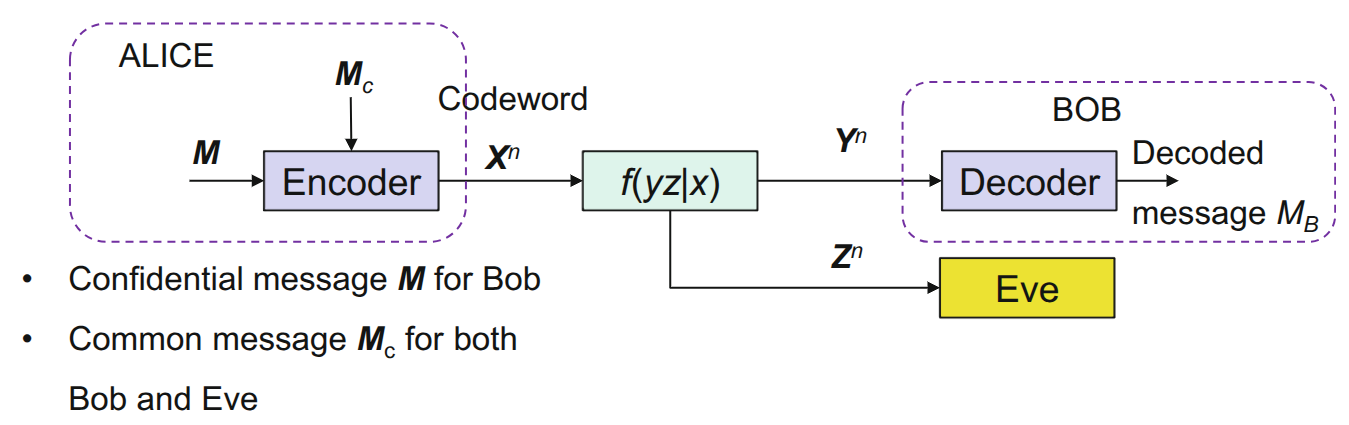
\includegraphics[width=0.8\textwidth]{chapters/figs/fig-1-5}
	\caption{مدل کانال پخش با پیام‌های محرمانه (\lr{BCC}).}
	\label{fig:1-5}
\end{figure}

یک کد شنود $(n, k)$ با نرخ $R = k/n$ توسط موارد زیر مشخص می‌شود \cite{1-3, 1-31}: (۱) مجموعه پیام‌های $M$ با اندازه $2^{nR}$، (۲) منبع تصادفی محلی $U$ با توزیع $f_U$، (۳) رمزگذاری که نگاشت پیام و یک تحقق تصادفی از منبع محلی را به یک کلمه کد انجام می‌دهد، و (۴) رمزگشایی که نگاشت کلمه دریافت‌شده به تخمین پیام را انجام می‌دهد. بزرگترین نرخ ارسالی که در آن هر دو شرط قابلیت اطمینان و محرمانگی به‌طور هم‌زمان برقرار باشند، معمولاً ظرفیت محرمانگی\LTRfootnote{Secrecy capacity} نامیده می‌شود. برای هر توزیع $f_x$ از $X$ از مجموعه‌ای از توزیع‌های $\mathcal{P}$ ($R \geq 0$) که برای آن‌ها $I(X, Y) \geq R$ است، واینر تابعی را تعریف کرده است که می‌توان آن را نرخ محرمانگی\LTRfootnote{Secrecy rate} نامید:

\begin{equation}
	SR(R) = \sup_{f_x \in \mathcal{P}(R)} [ I(X; Y) - I(X; Z) ].
	\label{eq:1-7}
\end{equation}
او همچنین نشان داد که نرخ محرمانگی\LTRfootnote{Secrecy rate} $SR(R)$ از بالا توسط ظرفیت کانال اصلی $C_m$ و از پایین توسط $C_m - C_e$ محدود می‌شود، که در آن $C_e$ ظرفیت آبشار کانال شنود اصلی است، یعنی:
\begin{equation}
	C_m - C_e \leq SR(R) \leq C_m.
	\label{eq:1-8}
\end{equation}
کانال شنود واینر توسط سیزار و کورنر تعمیم و بهبود یافت \cite{1-32} و مدل متناظر آن، که اکنون با نام کانال پخش با پیام‌های محرمانه (\lr{BCC})\LTRfootnote{Broadcast channel with confidential messages (BCC)} شناخته می‌شود، در شکل \ref{fig:1-5} ارائه شده است. فرض می‌شود که کانال پخش، گسسته و بدون حافظه\LTRfootnote{Discrete memoryless} باشد و توسط الفبای ورودی $\mathcal{X}$، الفباهای خروجی $\mathcal{Y}$ و $\mathcal{Z}$ (به‌ ترتیب مربوط به باب و ایو) و \lr{PDF} انتقال $f(yz|x)$ مشخص گردد. بنابراین، خودِ کانال توسط یک \lr{PDF} مشترک برای مشاهدات باب و ایو، $f(yz|x)$، به شرط ورودی کانال مدل‌سازی می‌شود. در این سناریو، آلیس مایل است یک پیام عمومی $M_c$ را برای هر دو گیرنده باب و ایو، و یک پیام محرمانه $M$ را برای باب پخش کند. کد تصادفی متناظر $\mathcal{C}_n$ با طول کلمه کد $n$ از موارد زیر تشکیل شده است:

\begin{itemize}
	\item دو مجموعه پیام: مجموعه پیام‌های عمومی و مجموعه پیام محرمانه.
	\item تابع رمزگذاری (تصادفی) که جفت پیام محرمانه-عمومی را به یک کلمه کد نگاشت می‌کند.
	\item دو تابع رمزگشایی: اولی که بردار مشاهده $\bm{y}^n$ را به جفت پیام تخمینی نگاشت می‌کند، در حالی که دومی بردار مشاهده $\bm{z}^n$ را به تخمین پیام عمومی نگاشت می‌نماید.
\end{itemize}

سیزار و کورنر نتیجه‌ای را اثبات کردند \cite{1-32} که بر اساس آن ظرفیت محرمانگی\LTRfootnote{Secrecy capacity} زمانی که نرخ پیام عمومی صفر تنظیم شود، به‌صورت تفاضل اطلاعات متقابل برای پیوندهای آلیس-باب و آلیس-ایو تعیین می‌شود، یعنی:
\begin{equation}
	C_s = \max_{\stackrel{f_{VX}}{V \to X \to YZ}} [ I(V; Y) - I(V; Z) ],
	\label{eq:1-9}
\end{equation}
که در آن بیشینه‌سازی روی تمام توزیع‌های مشترک ممکن $f_{VX}(v, x)$ انجام می‌شود و $V$، $X$ و $YZ$ یک زنجیره مارکوف $V \to X \to YZ$ را تشکیل می‌دهند. به‌وضوح، ظرفیت محرمانگی زمانی که کانال باب نویز کمتری نسبت به کانال ایو داشته باشد، یعنی $I(X; Y) > I(X; Z)$، اکیداً مثبت است. به‌ویژه، با قرار دادن $V = X$، عبارت ظرفیت محرمانگی به‌صورت $C_s = \max_{f_X} [ I(X; Y) - I(X; Z) ]$ در می‌آید که در صورت برقرار بودن $I(X; Y) > I(X; Z)$، اکیداً مثبت خواهد بود.
در مقایسه با رویکردهای رمزنگاری متداول که در آن‌ها از طرح‌های کدگذاری کنترل خطا (\lr{ECC})\LTRfootnote{Error control coding (ECC)} قوی برای فراهم‌سازی ارتباطات قابل‌اطمینان استفاده می‌شود، ارسال در سناریوی امنیت لایه فیزیکی (\lr{PLS}) باید به‌طور هم‌زمان قابل‌اطمینان و امن باشد. این امر نشان می‌دهد که باید کلاس‌های متفاوتی از کدهای کانال توسعه یابند. متناوباً، مشابه با \lr{QKD}، می‌توان از تصادفی بودن کانال برای تولید کلید بهره‌برداری کرد و این رویکرد معمولاً با عنوان توافق کلید مخفی\LTRfootnote{Secret-key agreement} شناخته می‌شود؛ این مفهوم در شکل \ref{fig:1-6} با الهام از مراجع \cite{1-2, 1-3, 1-6} توصیف شده است. آلیس و باب ظرفیت کانال آلیس-باب (که با نام ظرفیت کانال اصلی نیز شناخته می‌شود) $C_M$ و ظرفیت محرمانگی\LTRfootnote{Secrecy capacity} $C_S$ را که به‌صورت تفاضل بین ظرفیت کانال اصلی و ظرفیت کانال شنود $C_E$ تعریف می‌شود، پایش می‌کنند. زمانی که ظرفیت محرمانگی به‌خوبی بالاتر از مقدار آستانه $C_{S,tsh}$ و ظرفیت کانال اصلی به‌خوبی بالاتر از مقدار آستانه $C_{M,tsh}$ باشد، آلیس نمادهای با شکل گاوسی $X$ را برای باب ارسال می‌کند. هنگامی که هر دو ظرفیت محرمانگی و ظرفیت کانال اصلی به دلیل محوشدگی عمیق\LTRfootnote{Deep fading} در کانال‌های بی‌سیم یا اثرات تلاطم اتمسفری\LTRfootnote{Atmospheric turbulence} در کانال‌های نوری فضای آزاد پایین‌تر از آستانه‌های مربوطه قرار می‌گیرند، آلیس و باب مصالحه اطلاعات\LTRfootnote{Information reconciliation} نمادهای ارسال‌شده قبلی را انجام می‌دهند که بر پایه یک طرح \lr{ECC} قوی است تا اطمینان حاصل شود خطاهای وارد شده توسط کانال یا ایو قابل اصلاح هستند. مشابه طرح‌های \lr{QKD} \cite{1-7, 1-8, 1-9, 1-10, 1-11}، می‌توان از یک کد بررسی توازن کم‌چگال (\lr{LDPC})\LTRfootnote{Low-density parity-check (LDPC)} سیستماتیک استفاده کرد (که بر بیت‌های اطلاعات تأثیری نمی‌گذارد اما بیت‌های توازن\LTRfootnote{Parity bits} مرتبط جبری با بیت‌های اطلاعات را تولید می‌کند) تا بیت‌های توازن تولید شده و از طریق یک کانال عمومی احرازهویت‌شده\LTRfootnote{Authenticated public channel} ارسال گردند. طرح‌های مصالحه اطلاعات مستقیم و معکوس وجود دارند. در مصالحه مستقیم که در شکل \ref{fig:1-6} نشان داده شده است، آلیس رمزگذاری \lr{LDPC} را انجام داده و بیت‌های توازن را برای باب می‌فرستد. باب رمزگشایی \lr{LDPC} را برای به‌دست آوردن کلید صحیح $X$ انجام می‌دهد. در مصالحه معکوس، باب به جای آلیس رمزگذاری \lr{LDPC} را انجام می‌دهد. سپس تقویت حریم خصوصی\LTRfootnote{Privacy amplification} بین آلیس و باب انجام می‌شود تا از $X$ مجموعه کوچک‌تری از بیت‌های $K$ (کلید نهایی) استخراج گردد که همبستگی آن با رشته ایو پایین‌تر از یک آستانه مطلوب باشد \cite{1-9, 1-10, 1-11, 1-33}. یکی از راه‌های انجام تقویت حریم خصوصی، استفاده از توابع هش سراسری\LTRfootnote{Universal hash functions} $G$ است \cite{1-9, 1-10, 1-11, 1-33}، که مجموعه رشته‌های $n$-بیتی $X$ را به مجموعه رشته‌های $m$-بیتی $K$ نگاشت می‌کنند، به‌طوری که برای هر دو رشته متمایز $X_1$ و $X_2$ از مجموعه کلیدهای اصلاح‌شده، زمانی که نگاشت $g$ به‌صورت یکنواخت و تصادفی از $G$ انتخاب شود، احتمال برقراری $g(X_1) = g(X_2)$ بسیار پایین باشد. به‌طور معمول دو نوع مدل برای توافق کلید مخفی در نظر گرفته می‌شود \cite{1-34}:

\begin{itemize}
	\item \textbf{مدل نوع منبع\LTRfootnote{Source-type model}:} که در آن ترمینال‌ها خروجی همبسته منبع تصادفی را بدون داشتن کنترل بر آن مشاهده می‌کنند.
	\item \textbf{مدل نوع کانال\LTRfootnote{Channel-type model}:} که در آن یک ترمینال نمادهای تصادفی را با استفاده از یک کانال پخش برای ترمینال‌های دیگر ارسال می‌کند. این سناریو مشابه مدل کانال شنود با کانال بازخورد است که یک کانال عمومی احرازهویت‌شده بدون نویز محسوب می‌شود.
\end{itemize}

هر دوی این مدل‌ها بسیار شبیه به \lr{QKD} هستند \cite{1-7, 1-8, 1-9, 1-10, 1-11, 1-35, 1-36, 1-37, 1-38}، با این تفاوت که کلید خام در \lr{PLS} از طریق کانال کلاسیک ارسال می‌شود، در حالی که در \lr{QKD} از طریق کانال کوانتومی ارسال می‌گردد. پروتکل‌های توافق کلید مخفی علاوه بر شرط قابلیت اطمینان و شرط محرمانگی، باید شرط یکنواختی\LTRfootnote{Uniformity condition} را نیز ارضا کنند، که تضمین می‌کند کلید مخفی به‌طور یکنواخت در مجموعه مربوطه توزیع شده است. نرخی که کلید مخفی در آن تولید می‌شود را می‌توان مشابه \lr{QKD}، نرخ کلید مخفی (\lr{SKR})\LTRfootnote{Secret-key rate (SKR)} نامید. اگر پروتکل‌ها از پیام‌های عمومی ارسالی تنها در یک جهت (یا از آلیس به باب و یا از باب به آلیس) بهره‌برداری کنند، گفته می‌شود \lr{SKR} متناظر با ارتباط یک‌طرفه\LTRfootnote{One-way communication} دستیابی‌پذیر است؛ در غیر این صورت، گفته می‌شود \lr{SKR} با ارتباط دوطرفه\LTRfootnote{Two-way communication} دستیابی‌پذیر است. ما می‌گوییم نرخ کلید مخفی $R$ دستیابی‌پذیر است اگر دنباله‌ای از پروتکل‌های تولید کلید مخفی وجود داشته باشد که هر سه شرط (محدودیت) را در حالت $n \to \infty$ ارضا کند. سوپریمم نرخ‌های \lr{SKR} دستیابی‌پذیر معمولاً ظرفیت کلید مخفی\LTRfootnote{Secret-key capacity} نامیده شده و در اینجا با $C_{SK}$ نشان داده می‌شود. با فرض ارتباط دوطرفه روی کانال عمومی احرازهویت‌شده، استخراج یک عبارت دقیق برای $C_{SK}$ دشوار است؛ با این حال، بر اساس مراجع \cite{1-34, 1-39}، می‌توان آن را به‌صورت زیر از هر دو طرف محدود کرد:
\begin{equation}
	\max_{f_X} [ \max(I(X; Y) - I(X; Z), I(Y; X) - I(Y; Z)) ] \leq C_{SK} \leq \max_{f_X} I(X; Y|Z)
	\label{eq:1-10}
\end{equation}
جمله کران بالا نشان‌دهنده ظرفیت کلید مخفی در حالتی است که باب به مشاهدات ایو دسترسی داشته باشد. جمله کران پایین $\max[I(X; Y) - I(X; Z)]$ نشان‌دهنده به‌کارگیری مصالحه مستقیم\LTRfootnote{Direct reconciliation} است، در حالی که جمله کران پایین دیگر یعنی $\max[I(Y; X) - I(Y; Z)]$ نشان می‌دهد که به جای آن از مصالحه معکوس\LTRfootnote{Reverse reconciliation} استفاده شده است.
به‌طور خلاصه، \lr{PLS} به روش‌ها و الگوریتم‌های مختلفی مربوط می‌شود که امنیت را با بهره‌برداری از ویژگی‌های محیط فیزیکی فراهم می‌کنند. جزئیات بیشتر درباره طرح‌های مختلف \lr{PLS} را می‌توان در سایر فصل‌ها یافت.

\section{مبانی توزیع کلید کوانتومی (QKD)}
\label{sec:1-2}
اخیراً دستاوردهای قابل‌توجهی در محاسبات کوانتومی حاصل شده است \cite{1-9, 1-10, 1-11}. شرکت‌های بسیاری در حال حاضر بر روی توسعه کامپیوترهای کوانتومی با مقیاس متوسط کار می‌کنند. با توجه به اینکه اکثر سیستم‌های رمزنگاری به فرض دشواری محاسباتی\LTRfootnote{Computational hardness assumption} وابسته هستند، محاسبات کوانتومی چالشی جدی برای سیستم‌های امنیت سایبری مدرن محسوب می‌شود. به‌عنوان مثال، برای شکستن پروتکل \lr{RSA} \cite{1-26}، نیاز است که دوره تناوب $r$ تابع $f(x) = m^x \pmod n = f(x+r)$ تعیین شود ($r = 0, 1, \dots, 2^l - 1$؛ و $m$ عددی صحیح و کوچک‌تر از $n-1$ است). این دوره تناوب در یکی از مراحل الگوریتم تجزیه شور تعیین می‌شود \cite{1-9, 1-10, 1-11, 1-27, 1-28, 1-29}.

توزیع کلید کوانتومی (\lr{QKD}) با رمزگذاری متقارن\LTRfootnote{Symmetric encryption} را می‌توان به‌عنوان یکی از طرح‌های امنیت لایه فیزیکی تفسیر کرد که می‌تواند امنیت اثبات‌پذیری\LTRfootnote{Provable security} را در برابر حملات آغاز شده توسط کامپیوترهای کوانتومی فراهم کند \cite{1-35}. اولین طرح \lr{QKD} توسط بنت\LTRfootnote{Bennett} و براسارد\LTRfootnote{Brassard} معرفی شد که آن را در سال ۱۹۸۴ پیشنهاد کردند \cite{1-7, 1-8} و اکنون با نام پروتکل \lr{BB84} شناخته می‌شود. امنیت \lr{QKD} توسط قوانین مکانیک کوانتومی تضمین شده است. درجات آزادی\LTRfootnote{Degrees of freedom (DOF)} مختلف فوتون مانند قطبش، زمان، فرکانس، فاز و تکانه زاویه‌ای مداری\LTRfootnote{Orbital angular momentum} را می‌توان برای پیاده‌سازی پروتکل‌های مختلف \lr{QKD} به کار گرفت. به‌طور کلی، بسته به استراتژی اعمال شده در سمت باب، دو طرح کلی \lr{QKD} وجود دارد: \lr{QKD} با متغیر گسسته\LTRfootnote{Discrete variable (DV)} (\lr{DV-QKD}) و \lr{QKD} با متغیر پیوسته\LTRfootnote{Continuous variable (CV)} (\lr{CV-QKD}). در طرح‌های \lr{DV-QKD}، یک آشکارساز تک‌فوتون\LTRfootnote{Single-photon detector (SPD)} (\lr{SPD}) در سمت باب به کار می‌رود، در حالی که در \lr{CV-QKD} مؤلفه‌های مربعی میدان\LTRfootnote{Field quadratures} با کمک آشکارسازی هموداین/هتروداین\LTRfootnote{Homodyne/heterodyne detection} اندازه‌گیری می‌شوند. طرح \lr{DV-QKD} با به‌کارگیری قضیه کپی‌ناپذیری\LTRfootnote{No-cloning theorem} و قضیه تمایزناپذیری\LTRfootnote{Indistinguishability} حالت‌های کوانتومی دلخواه به امنیت غیرمشروط دست می‌یابد. قضیه کپی‌ناپذیری بیان می‌کند که حالت‌های کوانتومی دلخواه را نمی‌توان کپی کرد، که نشان‌دهنده این است که ایو نمی‌تواند حالت‌های کوانتومی غیرمتعامد\LTRfootnote{Non-orthogonal} را حتی با کمک کامپیوتر کوانتومی تکثیر کند. از سوی دیگر، قضیه دوم بیان می‌کند که حالت‌های غیرمتعامد را نمی‌توان به‌طور ابهام‌ناپذیر متمایز کرد. به‌ویژه، هنگامی که ایو با حالت‌های کوانتومی ارسالی تعامل برقرار می‌کند تا اطلاعاتی درباره بیت‌های ارسالی به‌دست آورد، به‌طور ناخواسته وفاداری\LTRfootnote{Fidelity} حالت‌های کوانتومی را مختل می‌کند که توسط باب شناسایی خواهد شد. از طرف دیگر، \lr{CV-QKD} از اصل عدم قطعیت\LTRfootnote{Uncertainty principle} بهره می‌برد که بیان می‌کند هر دو مؤلفه هم‌فاز\LTRfootnote{In-phase} و مربعی\LTRfootnote{Quadrature} حالت‌های همدوس را نمی‌توان به‌طور هم‌زمان با دقت کامل اندازه‌گیری کرد. ما همچنین می‌توانیم طرح‌های مختلف \lr{QKD} را در دو نوع «به کمک درهم‌تنیدگی» یا «آماده‌سازی-و-اندازه‌گیری»\LTRfootnote{Prepare-and-measure} طبقه‌بندی کنیم.

پژوهش در \lr{QKD} در حال شتاب گرفتن است، به‌ویژه پس از اولین نمایش \lr{QKD} ماهواره به زمین \cite{1-36}. اخیراً \lr{QKD} در مسافت ۴۰۴ کیلومتری از فیبر نوری با تلفات بسیار کم نمایش داده شده است؛ با این حال، نرخ کلید امن بسیار پایینی ($3.2 \times 10^{-4}$ بیت بر ثانیه) داشت. با توجه به اینکه حالت‌های کوانتومی قابل تقویت نیستند، تضعیف فیبر مسافت را محدود می‌کند. از سوی دیگر، زمان مرده\LTRfootnote{Deadtime} (مدت زمانی که یک \lr{SPD} به دلیل زمان بازیابی طولانی نسبت به فوتون‌های ورودی پاسخگو نیست) در \lr{SPD}ها که معمولاً در محدوده ۱۰ تا ۱۰۰ نانوثانیه است، نرخ باود\LTRfootnote{Baud rate} و در نتیجه نرخ کلید امن را محدود می‌کند. طرح‌های \lr{CV-QKD} از آنجا که از آشکارسازی هموداین/هتروداین استفاده می‌کنند، محدودیت زمان مرده ندارند؛ اما مسافت‌های معمول آن‌ها کوتاه‌تر است.

آلیس و باب با ارسال حالت‌های کیوبیت غیرمتعامد بین خود و بررسی اختلال در حالت ارسالی ناشی از کانال یا فعالیت ایو، می‌توانند حد بالایی برای نویز یا شنود در کانال ارتباطی کوانتومی خود تعیین کنند \cite{1-9}. آستانه حداکثر نرخ خطای تحمل‌پذیر توسط بازدهی بهترین مراحل پس‌پردازش تعیین می‌شود \cite{1-9}. پروتکل‌های \lr{QKD} را می‌توان به چندین دسته کلی تقسیم کرد:
\begin{itemize}
	\item \textbf{\lr{QKD} وابسته به دستگاه\LTRfootnote{Device-dependent QKD}:} که در آن معمولاً منبع کوانتومی در سمت آلیس و آشکارساز کوانتومی در سمت باب قرار دارد. کلاس‌های محبوب شامل \lr{DV-QKD}، \lr{CV-QKD}، \lr{QKD} به کمک درهم‌تنیدگی (\lr{EA}) و مرجع فاز توزیع‌شده\LTRfootnote{Distributed phase reference} است. برای \lr{EA-QKD}، منبع درهم‌تنیده را می‌توان در میانه کانال قرار داد تا مسافت ارسال افزایش یابد.
	\item \textbf{\lr{QKD} مستقل از دستگاه منبع:} که در آن منبع کوانتومی در سمت چارلی (ایو) قرار داده می‌شود، در حالی که آشکارسازهای کوانتومی در هر دو سمت آلیس و باب هستند.
	\item \textbf{\lr{QKD} مستقل از دستگاه اندازه‌گیری (\lr{MDI-QKD}):} که در آن آشکارسازهای کوانتومی در سمت چارلی (ایو) قرار می‌گیرند، در حالی که منابع کوانتومی در هر دو سمت آلیس و باب قرار دارند. حالت‌های کوانتومی در هر دو سمت آلیس و باب آماده‌سازی شده و به سمت آشکارسازهای چارلی ارسال می‌شوند. چارلی اندازه‌گیری‌های حالت بل\LTRfootnote{Bell state measurements} جزئی را انجام داده و زمانی که حالت بل جزئی مورد نظر شناسایی شد، آن را اعلام می‌کند؛ جزئیات بیشتر در فصل‌های بعدی ارائه خواهد شد.
\end{itemize}

\lr{QKD} می‌تواند به امنیت غیرمشروط\LTRfootnote{Unconditional security} دست یابد، به این معنی که امنیت آن را می‌توان بدون اعمال هیچ‌گونه محدودیتی بر توان محاسباتی یا استراتژی شنود ایو، تأیید کرد. کران‌های مربوط به نرخ کسر\LTRfootnote{Fraction rate} به مراحل پس‌پردازش کلاسیک\LTRfootnote{Classical postprocessing} بستگی دارد. رایج‌ترین روش، پس‌پردازش یک‌طرفه\LTRfootnote{One-way postprocessing} است که در آن آلیس یا باب کلید مرجع را در اختیار دارد و اطلاعات کلاسیک را از طریق کانال عمومی برای طرف دیگر ارسال می‌کند، در حالی که طرف مقابل بدون ارائه بازخورد، فرآیند خاصی را روی داده‌ها انجام می‌دهد. معمول‌ترین پردازش یک‌طرفه شامل دو مرحله است: مصالحه اطلاعات\LTRfootnote{Information reconciliation} و تقویت حریم خصوصی\LTRfootnote{Privacy amplification}. عبارت مربوط به کسر مخفی\LTRfootnote{Secret fraction} که از طریق پس‌پردازش یک‌طرفه به‌دست می‌آید، بسیار شبیه به طرح‌های \lr{PLS} کلاسیک است و به‌صورت زیر داده می‌شود:
\begin{equation}
	r = I(\bm{A}; \bm{B}) - \min_{\text{Eve's strategies}} (I_{EA}, I_{EB})
	\label{eq:1-11}
\end{equation}
که در آن $I(\bm{A}; \bm{B})$ اطلاعات متقابل\LTRfootnote{Mutual information} بین آلیس و باب است، در حالی که جمله دوم متناظر با اطلاعات ایو ($I_E$) درباره کلید خام آلیس یا باب است و کمینه‌سازی روی تمام استراتژی‌های شنود ممکن انجام می‌شود. آلیس و باب تصمیم خواهند گرفت که از مصالحه مستقیم یا معکوس استفاده کنند تا بتوانند اطلاعات ایو را کمینه نمایند.

اکنون استراتژی‌های مختلف شنود را که ایو ممکن است به کار گیرد و اطلاعات ایو $I_E$ را تعیین می‌کنند، شرح می‌دهیم. حملات مستقل (انفرادی) یا غیرهمدوس\LTRfootnote{Independent (individual) or incoherent attacks} محدودترین خانواده از حملات را تشکیل می‌دهند که در آن‌ها ایو به هر کیوبیت به‌طور مستقل حمله کرده و با اعمال استراتژی یکسان با هر کیوبیت تعامل می‌کند. علاوه بر این، او حالت‌های کوانتومی را پیش از انجام پس‌پردازش کلاسیک اندازه‌گیری می‌نماید. کران امنیت برای حملات غیرهمدوس مشابه کران امنیت در \lr{PLS} کلاسیک است که در آن اطلاعات متقابل بین آلیس و ایو به‌صورت زیر داده می‌شود:
\begin{equation}
	I_{EA} = \max_{\text{Eve's strategies}} I(\bm{A}; \bm{E})
	\label{eq:1-12}
\end{equation}
که در آن بیشینه‌سازی روی تمام استراتژی‌های شنود غیرهمدوس ممکن انجام می‌شود. تعریف مشابهی برای $I_{BE}$ نیز برقرار است.

حملات دسته‌جمعی\LTRfootnote{Collective attacks} نشان‌دهنده تعمیمی از حملات غیرهمدوس هستند، با این فرض که تعامل ایو با هر بیت کوانتومی (که با نام کیوبیت\LTRfootnote{Qubit} نیز شناخته می‌شود) نیز به‌صورت مستقل و با توزیع یکسان (\lr{i.i.d.})\LTRfootnote{Independent and identically distributed (i.i.d.)} است. با این حال، در این حملات ایو می‌تواند کیوبیت‌های کمکی\LTRfootnote{Ancilla qubits} خود را تا پایان مراحل پس‌پردازش کلاسیک در یک حافظه کوانتومی\LTRfootnote{Quantum memory} ذخیره کند. کران امنیت برای حملات دسته‌جمعی با فرض پس‌پردازش یک‌طرفه، توسط رابطه \eqref{eq:1-11} داده می‌شود که در آن اطلاعات ایو درباره دنباله آلیس بر اساس اطلاعات هولِوو\LTRfootnote{Holevo information} به‌صورت زیر تعیین می‌شود \cite{1-37, 1-38}:
\begin{equation}
	I_{EA} = \max_{\text{Eve's strategies}} \chi(\bm{A}; \bm{E})
	\label{eq:1-13}
\end{equation}
که در آن بیشینه‌سازی روی تمام استراتژی‌های شنود دسته‌جمعی ممکن انجام می‌شود. تعریف مشابهی نیز برای $I_{BE}$ برقرار است. این کران با نام کران دوتک-وینتر\LTRfootnote{Devetak-Winter bound} نیز شناخته می‌شود. اطلاعات هولِوو که در مرجع \cite{1-40} معرفی شده است، در اینجا به‌صورت زیر تعریف می‌گردد:
\begin{equation}
	\chi(\bm{A}; \bm{E}) = S(\rho_E) - \sum_{a} p(a) S(\rho_{E|a})
	\label{eq:1-14}
\end{equation}
که در آن $S(\rho)$ آنتروپی فون نویمان\LTRfootnote{von Neumann entropy} است که به‌صورت $S(\rho) = -\text{Tr}(\rho \log \rho) = -\sum_{i} \lambda_i \log \lambda_i$ تعریف می‌شود و در آن $\lambda_i$ مقادیر ویژه عملگر (حالت) چگالی\LTRfootnote{Density operator} $\rho$ هستند. عملگر چگالی برای بازنمایی مجموعه‌ای\LTRfootnote{Ensemble} از حالت‌های کوانتومی استفاده می‌شود که هر کدام با احتمالی معین رخ می‌دهند. (برای جزئیات بیشتر درباره عملگرهای چگالی به فصل \ref{chap:5} مراجعه کنید.) در رابطه \eqref{eq:1-14}، $p(a)$ نشان‌دهنده احتمال وقوع نماد $a$ از الفبای کلاسیک آلیس است، در حالی که $\rho_{E|a}$ عملگر چگالی متناظر با سیستم کمکی ایو است. در نهایت، $\rho_E$ حالت چگالی جزئی ایو است که به‌صورت $\rho_E = \sum_{a} p(a) \rho_{E|a}$ تعریف می‌شود. به عبارت دیگر، اطلاعات هولِوو متناظر با میانگین کاهش در آنتروپی فون نویمان است، با این فرض که می‌دانیم $\rho_E$ چگونه آماده‌سازی شده است.

\section{سازمان‌دهی کتاب}
\label{sec:1-3}
این کتاب به‌صورت زیر سازمان‌دهی شده است. در پایان هر فصل، مجموعه‌ای از مسائل برای کمک به خواننده در دستیابی به درک عمیق‌تر از مفاهیم شرح داده شده در آن فصل ارائه شده است. پس از مقدمه، در فصل \ref{chap:2}، مفاهیم نظریه اطلاعات\LTRfootnote{Information theory} کلاسیک به همراه کاربرد متناظر آن‌ها در کانال‌های محوشدگی\LTRfootnote{Fading channels} و کانال‌های دارای حافظه\LTRfootnote{Channels with memory} ارائه می‌شوند. این فصل مبانی نظریه اطلاعات و کدگذاری را در سطحی فراهم می‌کند که برای دنبال کردن آسان مطالب کتاب مورد نیاز است. فصل با تعاریف آنتروپی، آنتروپی مشترک، آنتروپی شرطی، آنتروپی نسبی\LTRfootnote{Relative entropy}، اطلاعات متقابل و ظرفیت کانال آغاز شده و با قضیه ظرفیت اطلاعات ادامه می‌یابد. ما درباره ظرفیت کانال در کانال‌های گسسته بدون حافظه، کانال‌های پیوسته و کانال‌های دارای حافظه بحث می‌کنیم. در رابطه با کانال‌های بی‌سیم، نحوه محاسبه ظرفیت کانال در کانال‌های محوشدگی هموار\LTRfootnote{Flat-fading} و گزینش‌گر فرکانس\LTRfootnote{Frequency-selective} را شرح می‌دهیم. همچنین استراتژی‌های مختلف بهینه و زیربهینه برای دستیابی به ظرفیت کانال، از جمله روش پر کردن آب\LTRfootnote{Water-filling method}، کدگذاری و رمزگشایی تسهیم‌شده، وارون‌سازی کانال و وارون‌سازی کانال کوتاه شده\LTRfootnote{Truncated channel inversion} را مورد بحث قرار می‌دهیم. علاوه بر این، استراتژی‌های مختلف برای محاسبه ظرفیت کانال بسته به آنچه از اطلاعات وضعیت کانال\LTRfootnote{Channel state information (CSI)} دانسته می‌شود، مطالعه می‌گردند. در ادامه، نحوه مدل‌سازی کانال دارای حافظه را توضیح داده و مدل مک‌میلان-خینچین\LTRfootnote{McMillan-Khinchin model} را برای ارزیابی ظرفیت کانال تشریح می‌کنیم. سپس، مبانی کدهای بلوکی خطی و به‌دنبال آن مبانی کدگذاری \lr{LDPC} باینری معرفی می‌شوند. پس از ملاحظات پایانی، مجموعه‌ای از مسائل ارائه شده است.

در فصل \ref{chap:3}، مبانی رمزنگاری متداول معرفی می‌شوند. ابتدا اصطلاحات پایه و طرح‌های رمزنگاری، شامل رمزنگاری متقارن و نامتقارن، رمزهای پایه مانند رمزهای جایگزینی\LTRfootnote{Substitution ciphers} و جابه‌جایی\LTRfootnote{Transposition ciphers}، و پد‌های یک‌بار مصرف معرفی می‌گردند. مفاهیم محرمانگی، احراز هویت و انکارناپذیری\LTRfootnote{Non-repudiation} مورد بحث قرار می‌گیرند و به‌دنبال آن حملات مختلف تحلیل رمز\LTRfootnote{Cryptanalytic attacks} مانند حملات فقط-رمزنگاشت\LTRfootnote{Ciphertext-only}، متن‌آشکار-معلوم\LTRfootnote{Known-plaintext}، متن‌آشکار-انتخابی\LTRfootnote{Chosen-plaintext}، رمزنگاشت-انتخابی\LTRfootnote{Chosen-ciphertext} و متن‌آشکار-انتخابی سازگار\LTRfootnote{Adaptive chosen-plaintext} بررسی می‌شوند. مفهوم امنیت کامل در ادامه معرفی شده و با امنیت محاسباتی مقایسه می‌گردد. در همان بخش، فاصله یکتایی\LTRfootnote{Unicity distance} و همچنین نقش فشرده‌سازی در رمزنگاری مورد بحث قرار می‌گیرد. سپس، توابع یک‌طرفه و توابع هش یک‌طرفه بررسی می‌شوند. فصل با چندین سیستم رمزنگاری کاربردی مرتبط، شامل سیستم‌های \lr{DES} و \lr{RSA} و همچنین توزیع کلید عمومی دیفی-هلمن\LTRfootnote{Diffie-Hellman} به پایان می‌رسد. در ادامه، ملاحظات پایانی و مجموعه‌ای از مسائل ارائه شده است.

فصل \ref{chap:4} به امنیت لایه فیزیکی اختصاص یافته است. فصل با بحثی درباره مسائل امنیتی آغاز شده و با معرفی امنیت نظریه-اطلاعاتی و مقایسه آن با امنیت محاسباتی ادامه می‌یابد. در همان بخش، معیارهای مختلف امنیت نظریه-اطلاعاتی، از جمله شرایط محرمانگی قوی و ضعیف معرفی می‌شوند. سپس، مدل کانال شنود واینر که با نام مدل کانال شنود تخریب‌شده نیز شناخته می‌شود، معرفی می‌گردد. در همان بخش، مفهوم ظرفیت محرمانگی و همچنین کدگذاری شنود آشیانه‌ای\LTRfootnote{Nested wiretap coding} معرفی می‌شود. علاوه بر این، کانال پخش با پیام‌های محرمانه معرفی شده و تعریف ظرفیت محرمانگی تعمیم داده می‌شود. سپس تمرکز به سمت تولید (توافق) کلید مخفی معطوف شده، مدل‌های نوع منبع و کانال معرفی می‌شوند و پروتکل‌های تولید کلید مخفی متناظر تشریح می‌گردند. بخش بعدی به کدگذاری برای سیستم‌های امنیت لایه فیزیکی، شامل کدگذاری برای سیستم‌های محرمانگی ضعیف و قوی اختصاص دارد. در رابطه با کدگذاری برای سیستم‌های محرمانگی ضعیف، توجه ویژه‌ای به کدگذاری \lr{LDPC} از نوع دو-لبه\LTRfootnote{Two-edge-type}، کدگذاری \lr{LDPC} پنچرشده\LTRfootnote{Punctured} و کدهای قطبی معطوف شده است. در مورد کدگذاری برای سیستم‌های محرمانگی قوی، تمرکز بر کدگذاری هم‌مجموعه‌ای\LTRfootnote{Coset coding} با کدهای \lr{LDPC} دوگان و کدگذاری مبتنی بر توابع هش/استخراج‌کننده\LTRfootnote{Extractor-based} است. سپس توجه به سمت مصالحه اطلاعات و تقویت حریم خصوصی معطوف می‌شود. در بخش \lr{PLS} کانال‌های بی‌سیم، موضوعات زیر پوشش داده می‌شوند: مبانی \lr{MIMO}، امنیت لایه فیزیکی در \lr{MIMO} بی‌سیم، و تولید کلید مخفی در شبکه‌های بی‌سیم. در بخش \lr{PLS} کانال‌های نوری، هر دو حوزه \lr{PLS} برای سیستم‌های مبتنی بر فیبرهای تسهیم‌سازی تقسیم فضایی\LTRfootnote{Spatial division multiplexing (SDM)} (\lr{SDM}) و سیستم‌های نوری فضای آزاد (\lr{FSO}) مورد بحث قرار می‌گیرند. ملاحظات پایانی در ادامه ارائه شده و به‌دنبال آن مجموعه‌ای از مسائل که برای درک بهتر مفاهیم شرح داده شده درج شده‌اند، می‌آید.


در فصل \ref{chap:5}، مفاهیم پایه پردازش اطلاعات کوانتومی\LTRfootnote{Quantum information processing}، نظریه اطلاعات کوانتومی و تصحیح خطای کوانتومی\LTRfootnote{Quantum error correction} برای درک بهتر سیستم‌های \lr{QKD} ارائه شده است. موضوعات زیر از حوزه پردازش اطلاعات کوانتومی پوشش داده شده‌اند: بردارهای حالت\LTRfootnote{State vectors}، عملگرها\LTRfootnote{Operators}، عملگرهای چگالی\LTRfootnote{Density operators}، اندازه‌گیری‌ها، دینامیک یک سیستم کوانتومی، اصل برهم‌نهی\LTRfootnote{Superposition principle}، موازی‌گرایی کوانتومی\LTRfootnote{Quantum parallelism}، قضیه کپی‌ناپذیری و درهم‌تنیدگی. مفاهیم زیر نیز از نظریه اطلاعات کوانتومی ارائه شده‌اند: اطلاعات هولِوو\LTRfootnote{Holevo information}، اطلاعات در دسترس\LTRfootnote{Accessible information}، کران هولِوو\LTRfootnote{Holevo bound}، آنتروپی شانون و آنتروپی فون نویمان، قضیه کدگذاری کوانتومی بدون نویز شوماخر\LTRfootnote{Schumacher’s noiseless quantum coding theorem} و قضیه هولِوو-شوماخر-وستمورلند\LTRfootnote{Holevo-Schumacher-Westmoreland theorem}. مفاهیم پایه تصحیح خطای کوانتومی نیز معرفی شده‌اند. در ادامه، فصل با مجموعه‌ای از مسائل به پایان می‌رسد.

فصل \ref{chap:6} به مبانی اپتیک کوانتومی و سیستم‌های متغیر پیوسته (\lr{CV}) اختصاص یافته است. ابتدا امواج الکترومغناطیسی، پتانسیل برداری و معادله موج معرفی شده و به‌دنبال آن، کوانتیزه کردن میدان‌های الکترومغناطیسی ارائه می‌شود. پس از معرفی عملگرهای مربعی\LTRfootnote{Quadrature operators}، حالت‌های فوک\LTRfootnote{Fock states}، همدوس\LTRfootnote{Coherent states} و فشرده\LTRfootnote{Squeezed states} را معرفی می‌کنیم. در ادامه، تقسیم‌کننده پرتو با استفاده از مفاهیم مکانیک کوانتومی توصیف شده و برای ساخت آشکارساز متعادل هموداین\LTRfootnote{Homodyne balanced detector} به کار می‌رود. در بخش بعدی، تداخل‌سنج ماخ-زندر کوانتومی معرفی می‌گردد. سپس، حالت‌های تابش گرمایی تشریح می‌شوند. فصل با معرفی مبانی نظریه اطلاعات کوانتومی گاوسی ادامه می‌یابد که در آن نمایش-$P$\LTRfootnote{P-representation} معرفی شده و برای نمایش نویز گرمایی و همچنین سیگنال حالت همدوس به‌همراه نویز گرمایی به کار می‌رود. علاوه بر این، حالت‌های گاوسی معرفی شده و به‌دنبال آن تعریف تابع ویگنر و ماتریس‌های همبستگی\LTRfootnote{Correlation matrices} ارائه می‌شود. زیربخش بعدی به تبدیل‌های گاوسی و کانال‌های گاوسی اختصاص دارد که عملگر تقسیم‌کننده پرتو، عملگر چرخش فاز و عملگرهای فشردگی به‌عنوان نمونه‌های شاخص آن‌ها بررسی می‌شوند. تجزیه گرمایی حالت‌های گاوسی موضوع بعدی است و آنتروپی فون نویمان برای حالت‌های گرمایی استخراج می‌شود. سپس تمرکز به سمت مبانی اپتیک کوانتومی غیرخطی معطوف شده و به‌ویژه اختلاط سه‌موج و اختلاط چهارموج به‌تفصیل شرح داده می‌شوند. در ادامه، تولید حالت‌های گاوسی توصیف شده و تولید حالت فشرده دو-مُدی\LTRfootnote{Two-mode squeeze state} به‌طور کامل مورد بحث قرار می‌گیرد. ماتریس‌های همبستگی برای حالت‌های گاوسی دو-مُدی و نحوه محاسبه مقادیر ویژه سیمپلکتیک\LTRfootnote{Symplectic eigenvalues} (مرتبط با محاسبه آنتروپی فون نویمان) در ادامه بررسی می‌شوند. اندازه‌گیری و آشکارسازی حالت‌های گاوسی با تأکید بر آشکارسازی هموداین، آشکارسازی هتروداین و اندازه‌گیری‌های جزئی مورد بحث قرار می‌گیرند. سپس ماتریس‌های کوواریانس برای حالت‌های گاوسی چندمُدی معرفی می‌شوند. در نهایت، ملاحظات پایانی و مجموعه‌ای از مسائل ارائه شده است.

فصل \ref{chap:7} به مبانی \lr{QKD} اختصاص دارد. فصل با توصیف تفاوت‌های کلیدی بین رمزنگاری متداول، \lr{PLS} کلاسیک و \lr{QKD} آغاز می‌شود. در بخش مبانی \lr{QKD}، پس از یک مرور تاریخی، انواع مختلف \lr{QKD} را مرور کرده و به‌اختصار مراحل معمول پس‌پردازش، یعنی مراحل مصالحه اطلاعات و تقویت حریم خصوصی را شرح می‌دهیم. در همان بخش، دو قضیه بنیادی که \lr{QKD} بر آن‌ها استوار است را ارائه می‌دهیم: قضیه کپی‌ناپذیری و قضیه عدم توانایی در تمایز ابهام‌ناپذیر حالت‌های کوانتومی غیرمتعامد. در بخش سیستم‌های \lr{QKD} با متغیر گسسته (\lr{DV})، پروتکل‌های \lr{BB84} و \lr{B92} و همچنین پروتکل‌های اکرت (\lr{E91}) و \lr{EPR} را به‌تفصیل توصیف می‌کنیم. در همان بخش، پروتکل کدگذاری فاز-زمان نیز شرح داده شده است. در رابطه با پروتکل‌های \lr{BB84}، نسخه‌های مختلف مناسب برای فناوری‌های گوناگون بررسی می‌شوند. در بخش امنیت \lr{QKD}، نرخ کلید مخفی به‌صورت حاصل‌ضرب نرخ کلید خام و نرخ کسری نمایش داده شده و به‌دنبال آن محدودیت‌های مختلف نرخ کلید خام توصیف می‌شوند. سپس، عبارت عمومی برای نرخ کسری ارائه شده و انواع استراتژی‌های شنود، شامل حملات انفرادی (مستقل یا غیرهمدوس)، حملات دسته‌جمعی و حملات همدوس\LTRfootnote{Coherent attacks}، و همچنین حملات هک کوانتومی/کانال جانبی تشریح می‌گردند. برای حملات انفرادی و همدوس، عبارات کسر مخفی متناظر شرح داده شده‌اند. بخش بعدی به تعاریف مختلف امنیت، از جمله مفهوم $\epsilon$-امنیت\LTRfootnote{$\epsilon$-security} اختصاص یافته است. سپس، عبارات عمومی برای طرح‌های \lr{DV-QKD} دوبعدی برای هر دو پروتکل آماده‌سازی-و-اندازه‌گیری و پروتکل‌های مبتنی بر حالت فریب استخراج می‌شوند. برای تسهیل توصیف پروتکل‌های \lr{QKD} با متغیر پیوسته (\lr{CV})، ابتدا مبانی اپتیک کوانتومی معرفی می‌شوند. در بخش پروتکل‌های \lr{CV-QKD}، هر دو نوع پروتکل مبتنی بر حالت‌های فشرده و حالت‌های همدوس تشریح می‌شوند. با توجه به اینکه تولید و دست‌کاری حالت‌های همدوس بسیار ساده‌تر است، پروتکل‌های مبتنی بر حالت همدوس با هر دو نوع آشکارسازی هموداین و هتروداین به‌تفصیل شرح داده شده‌اند. کسر مخفی برای هر دو پروتکل \lr{CV-QKD} مبتنی بر مصالحه مستقیم و معکوس استخراج شده است. علاوه‌ بر این، جزئیات جنبه‌های کاربردی پروتکل \lr{GG02} ارائه شده و محاسبه کسر مخفی برای حملات دسته‌جمعی مورد بحث قرار گرفته است. سپس، مفاهیم پایه پروتکل‌های \lr{QKD} مستقل از دستگاه اندازه‌گیری (\lr{MDI}) معرفی می‌شوند. در پایان فصل، ملاحظات پایانی و مجموعه‌ای از مسائل ارائه شده است.

فصل \ref{chap:8} در ادامه فصل \ref{chap:7} بوده و به پروتکل‌های \lr{QKD} با متغیر گسسته (\lr{DV}) اختصاص یافته است. فصل با توصیف پروتکل‌های \lr{BB84} و مبتنی بر حالت فریب، و ارزیابی عملکرد کسر محرمانگی آن‌ها برحسب مسافت دستیابی‌پذیر آغاز می‌شود. موضوع بعدی مربوط به امنیت پروتکل‌های \lr{DV-QKD} در شرایطی است که منابع محدود\LTRfootnote{Finite resources} هستند. ما مفهوم $\epsilon$-امنیت ترکیب‌پذیر\LTRfootnote{Composable $\epsilon$-security} را معرفی کرده و نحوه ارزیابی آن را برای هر دو نوع حمله دسته‌جمعی و همدوس شرح می‌دهیم. همچنین بحث می‌کنیم که چگونه مفاهیم صحت\LTRfootnote{Correctness} و محرمانگی را می‌توان برای دستیابی به کران‌های امنیتی محکم ترکیب کرد. سپس، پروتکل‌های \lr{BB84} و حالت فریب را برای فرض کلید محدود تحت اثرات تلاطم اتمسفری ارزیابی می‌کنیم. همچنین نحوه مواجهه با شرایط متغیر زمانی در کانال‌های نوری فضای آزاد توصیف می‌شود. سپس تمرکز به سمت پروتکل‌های \lr{QKD} با ابعاد بالا\LTRfootnote{High-dimensional (HD) QKD} معطوف شده و با توصیف انتخاب پایه‌های متقابلاً بدون سوگیری\LTRfootnote{Mutually unbiased bases (MUBs)} (\lr{MUBs}) و به‌دنبال آن معرفی حالت‌های بل تعمیم‌یافته آغاز می‌شود. سپس نحوه ارزیابی امنیت پروتکل‌های \lr{QKD} ابعاد بالا برای منابع محدود را شرح می‌دهیم. انواع پروتکل‌های \lr{QKD} ابعاد بالا، شامل کدگذاری فاز-زمان، کدگذاری زمان-انرژی، \lr{QKD} ابعاد بالا مبتنی بر \lr{OAM}، \lr{QKD} ابعاد بالا مبتنی بر توری‌های براگ فیبری\LTRfootnote{Fiber Bragg grating (FBGs)} (\lr{FBG}) و پروتکل‌های مبتنی بر توری‌های براگ موجبری\LTRfootnote{Waveguide Bragg gratings (WBGs)} (\lr{WBG}) توصیف می‌شوند. پس از ملاحظات پایانی، مجموعه‌ای از مسائل ارائه شده است.

فصل \ref{chap:9} به شرح تفصیلی طرح‌های \lr{CV-QKD}، به‌ویژه با مدولاسیون گاوسی و مدولاسیون گسسته اختصاص یافته است. به خواننده‌ای که با مبانی اپتیک کوانتومی و اصول سیستم‌های متغیر پیوسته (\lr{CV}) آشنا نیست، توصیه می‌شود ابتدا فصل \ref{chap:6} را مطالعه کند. در بخش مربوط به پروتکل‌های \lr{CV-QKD} با مدولاسیون گاوسی، پس از شرح کوتاهی از پروتکل‌های مبتنی بر حالت‌های فشرده، پروتکل‌های مبتنی بر حالت‌های همدوس با جزئیات کامل تشریح می‌شوند. ما این بخش را با توصیف هر دو نوع کانال ارسال بدون تلفات و با تلفات آغاز می‌کنیم. سپس هم‌ارزی بین پروتکل‌های آماده‌سازی-و-اندازه‌گیری\LTRfootnote{Prepare-and-measure (PM)} (\lr{PM}) و پروتکل‌های به کمک درهم‌تنیدگی\LTRfootnote{Entanglement-assisted} با مدولاسیون گاوسی مورد بحث قرار می‌گیرد. در ادامه، تمرکز به سمت محاسبه نرخ کلید مخفی تحت حملات دسته‌جمعی معطوف می‌شود. ابتدا محاسبه اطلاعات متقابل بین آلیس و باب بررسی شده و به‌دنبال آن محاسبه اطلاعات هولِوو بین ایو و باب، در هر دو مورد با فرض پروتکل \lr{PM} و مصالحه معکوس، انجام می‌شود. علاوه‌ بر این، حمله کپی‌کننده درهم‌تننده\LTRfootnote{Entangling-cloner attack} توصیف شده و استخراج اطلاعات هولِوو ایو-باب ارائه می‌گردد. سپس پروتکل به کمک درهم‌تنیدگی و استخراج اطلاعات هولِوو متناظر با آن تشریح می‌شود. در تمامی این استخراج‌ها، هر دو نوع آشکارسازی هموداین و هتروداین در نظر گرفته شده‌اند. همچنین برخی نتایج توصیفی \lr{SKR} مربوط به مدولاسیون گاوسی ارائه شده است. در بخش مربوط به \lr{CV-QKD} با مدولاسیون گسسته، پس از یک مقدمه کوتاه، پروتکل‌های \lr{CV-QKD} چهار-حالتی و هشت-حالتی را توصیف می‌کنیم. هر دو نوع پروتکل \lr{PM} و به کمک درهم‌تنیدگی مورد بحث قرار می‌گیرند. در ادامه، محاسبه \lr{SKR} برای مدولاسیون گسسته همراه با نتایج عددی توصیفی بررسی می‌شود. ما همچنین شرایطی را که در آن مدولاسیون گسسته می‌تواند عملکرد بهتری نسبت به مدولاسیون گاوسی داشته باشد، شناسایی می‌کنیم. در بخش طرح \lr{CV-QKD} به کمک \lr{RF}\LTRfootnote{RF-assisted}، یک طرح کلی به کمک \lr{RF} را توصیف می‌کنیم که برای طرح‌های مدولاسیون دوبعدی دلخواه، از جمله \lr{M-ary PSK} و \lr{M-ary QAM}، قابل اعمال است. این طرح در مقایسه با پروتکل‌های \lr{CV-QKD} متداول با مدولاسیون گسسته، تاب‌آوری بهتری نسبت به نویز فاز لیزر و نوسانات آفست فرکانسی نشان می‌دهد. سپس نحوه افزایش \lr{SKR} از طریق رویکرد موازی‌سازی\LTRfootnote{Parallelization} را مورد بحث قرار می‌دهیم. بخش نهایی فصل ملاحظات پایانی مرتبط را ارائه داده و به‌دنبال آن مسائل فصل می‌آیند.

فصل \ref{chap:10} به طرح‌های \lr{QKD} با متغیر گسسته (\lr{DV}) و متغیر پیوسته (\lr{CV}) که اخیراً پیشنهاد شده‌اند، اختصاص دارد. فصل با توصیف اثر هونگ-او-ماندل و اندازه‌گیری‌های حالت بل\LTRfootnote{Bell state measurements (BSMs)} (\lr{BSM}) فوتونی آغاز می‌شود. هر دو نوع \lr{BSM} مبتنی بر حالت‌های قطبش و حالت‌های بازه-زمانی\LTRfootnote{Time-bin} معرفی می‌شوند. سپس پروتکل‌های \lr{BB84} و حالت فریب به‌طور مختصر بازبینی می‌شوند. موضوع بعدی در این فصل به پروتکل‌های \lr{QKD} مستقل از دستگاه اندازه‌گیری (\lr{MDI}) اختصاص یافته است. هر دو پروتکل \lr{MDI-QKD} مبتنی بر حالت‌های قطبش و حالت‌های فاز-زمان تشریح می‌شوند. علاوه‌ بر این، پروتکل‌های \lr{QKD} میدان-دوقلو\LTRfootnote{Twin-field (TF)-QKD} (\lr{TF}) توصیف می‌شوند که قادر به شکستن کران پیراندولا-لورنزا-اوتاویانی-بانکی (\lr{PLOB}) روی نرخ کلید خطی هستند. سپس پروتکل \lr{CV-QKD} نورافکن\LTRfootnote{Floodlight (FL)} (\lr{FL}) توصیف می‌شود که قادر به دستیابی به نرخ‌های کلید مخفی رکوردشکن است. در ادامه، طرح \lr{CV-QKD} مبتنی بر گیرنده کرامرز-کرونیگ\LTRfootnote{Kramers-Kronig (KK)-receiver} (\lr{KK}) معرفی می‌گردد که نشان‌دهنده طرحی با \lr{SKR} بالا و پیچیدگی کم است. سپس طرح \lr{CV-QKD}ای تشریح می‌شود که در آن مصالحه اطلاعات از طریق یک پیوند به کمک درهم‌تنیدگی انجام می‌گیرد. در نهایت ملاحظات پایانی ارائه شده و مجموعه‌ای از مسائل برای کمک به خوانندگان در جهت کسب درک عمیق‌تر آورده شده است.

فصل \ref{chap:11} به مخابرات پنهان\LTRfootnote{Covert communications} که با نام احتمال پایین آشکارسازی/شنود\LTRfootnote{Low probability of detection/intercept} نیز شناخته می‌شود، و همچنین مخابرات رادارگریز\LTRfootnote{Stealth communications} اختصاص یافته است و اینکه چگونه این روش‌ها می‌توانند نرخ کلید مخفی را برای کاربردهای \lr{QKD} بهبود بخشند. فصل با مقدمه‌ای کوتاه بر مخابرات پنهان آغاز شده و با توصیف تفاوت‌های آن‌ها نسبت به پنهان‌نگاری\LTRfootnote{Steganography} ادامه می‌یابد. یکی از فناوری‌های کلیدی برای توانمندسازی مخابرات پنهان در کانال‌های بی‌سیم، یعنی مفهوم طیف گسترده\LTRfootnote{Spread spectrum}، در ادامه معرفی می‌شود. سپس، بررسی دقیق مخابرات پنهان در یک کانال نویز گاوسی سفید جمع‌شونده (\lr{AWGN}) ارائه شده و قانون ریشه دوم\LTRfootnote{Square root law} استخراج می‌گردد. اهمیت آزمون فرض\LTRfootnote{Hypothesis testing} در مخابرات پنهان نیز مورد بحث قرار می‌گیرد. سپس مخابرات پنهان در کانال‌های گسسته بدون حافظه بررسی می‌شود. موضوع بعدی به رویکردهای مختلف برای غلبه بر قانون ریشه دوم مربوط است، از جمله استفاده از مسدودکننده (جمر) دوست\LTRfootnote{Friendly jammer} که توان نویز را تغییر می‌دهد تا بتوان بر قانون ریشه دوم غلبه کرد و به نرخ پنهان مثبت دست یافت. مفهوم محرمانگی مؤثر\LTRfootnote{Effective secrecy} در ادامه معرفی می‌شود که یک معیار محرمانگی جدید است و تعریف آن شامل هر دو شرط محرمانگی قوی و مخابرات رادارگریز می‌باشد. سپس، مفهوم مخابرات پنهان/رادارگریز در سیستم‌های مخابرات نوری به کار گرفته می‌شود. ما در ادامه توصیف می‌کنیم که چگونه مفهوم پنهان‌سازی می‌تواند در مرحله مصالحه اطلاعات در \lr{QKD} اعمال شود تا به‌طور هم‌زمان نرخ کلید مخفی بهبود یافته و مسافت ارسال افزایش یابد. سپس نتایج تجربی مربوط به احتمال پایین شنود و مخابرات پنهان که در کانال‌های با تلاطم اتمسفری قوی عمل می‌کنند، ارائه می‌شود. بخش پایانی فصل را خلاصه کرده و مجموعه‌ای از مسائل در انتهای آن قرار گرفته است.

فصل \ref{chap:12} به مفاهیم رمزنگاری پسا‌کوانتومی\LTRfootnote{Post-quantum cryptography (PQC)} (\lr{PQC}) مربوط می‌شود. پس از مقدمه‌ای کوتاه، مفاهیم رمزنگاری مبتنی بر مشبکه\LTRfootnote{Lattice-based cryptography} زیر تشریح می‌شوند: رمزنگاری مبتنی بر یادگیری با خطا\LTRfootnote{Learning with errors (LWE)} (\lr{LWE}) ماتی\LTRfootnote{Module}، رمزنگاری مبتنی بر \lr{LWE} حلقوی، امضاهای دیجیتال مبتنی بر مشبکه و توابع هش مبتنی بر مشبکه. علاوه‌ بر این، مفاهیم رمزنگاری مبتنی بر کد\LTRfootnote{Code-based cryptography} با تمرکز بر طرح رمزگذاری مک‌الیس\LTRfootnote{McEliece}، سیستم رمزنگاری نیدرایتر\LTRfootnote{Niederreiter} و رمزگذاری مبتنی بر کدگذاری \lr{QC-LDPC} شبه‌دوری تشریح می‌شوند. در بخش بعدی، مفاهیم ترکیبی \lr{QKD-PQC} توصیف می‌شوند که در آن‌ها \lr{QKD} و \lr{PQC} به‌صورت تعاملی عمل می‌کنند. موضوع بعدی مربوط به رمزنگاری مبتنی بر هش\LTRfootnote{Hash-based cryptography} است؛ این بخش با مفاهیم پایه رمزنگاری مبتنی بر هش شامل طرح امضای یک‌بار مصرف لمپورت\LTRfootnote{Lamport} آغاز می‌شود. دو طرح رمزنگاری مبتنی بر هش مرتبط تشریح می‌شوند: طرح امضای یک‌بار مصرف وینترنیتز\LTRfootnote{Winternitz} (\lr{W-OTS}) و طرح امضای مرکل\LTRfootnote{Merkle} (\lr{MMS}) که برای امضاهای چندبار مصرف قابل اعمال است. برخی مفاهیم مرتبط با رمزنگاری چندمتغیره\LTRfootnote{Multivariate cryptography} در ادامه توصیف می‌شوند. پس از ملاحظات پایانی، مجموعه‌ای از مسائل ارائه شده است.

در پیوست، برخی مطالب پیش‌زمینه مانند مبانی جبر مجرد\LTRfootnote{Abstract algebra fundamentals} ارائه شده است که به خوانندگان ناآشنا کمک می‌کند مفاهیم امنیت لایه فیزیکی، \lr{QKD} و \lr{PQC} را بهتر درک کنند.
	% !TeX root = ../quantum.tex
\chapter{امنیت لایه فیزیکی}
\label{chap:4}

\section*{چکیده}
این فصل به امنیت لایه فیزیکی (\lr{PLS}) اختصاص یافته است. فصل با بحثی درباره مسائل امنیتی آغاز شده و با مقدمه‌ای بر امنیت نظریه-اطلاعاتی\LTRfootnote{Information-theoretic security} و مقایسه آن با امنیت محاسباتی\LTRfootnote{Computational security} ادامه می‌یابد. در همان بخش، معیارهای مختلف امنیت نظریه-اطلاعاتی، از جمله شرایط محرمانگی قوی\LTRfootnote{Strong secrecy} و ضعیف\LTRfootnote{Weak secrecy} معرفی می‌شوند. سپس، مدل کانال شنود\LTRfootnote{Wiretap channel} واینر\LTRfootnote{Wyner} که با نام مدل کانال شنود تخریب‌شده\LTRfootnote{Degraded wiretap channel} نیز شناخته می‌شود، معرفی می‌گردد. در همان بخش، مفهوم ظرفیت محرمانگی\LTRfootnote{Secrecy capacity} و همچنین کدگذاری شنود آشیانه‌ای\LTRfootnote{Nested wiretap coding} بررسی می‌شود. علاوه بر این، کانال پخش با پیام‌های محرمانه\LTRfootnote{Broadcast channel with confidential messages} معرفی شده و تعریف ظرفیت محرمانگی تعمیم می‌یابد. سپس تمرکز به سمت تولید (توافق) کلید مخفی\LTRfootnote{Secret-key generation (agreement)} معطوف شده، مدل‌های نوع منبع و نوع کانال معرفی می‌شوند و پروتکل‌های تولید کلید مخفی متناظر تشریح می‌گردند. بخش بعدی به کدگذاری برای سیستم‌های امنیت لایه فیزیکی، شامل کدگذاری برای هر دو سیستم محرمانگی ضعیف و قوی اختصاص دارد. در رابطه با کدگذاری برای سیستم‌های محرمانگی ضعیف، توجه ویژه‌ای به کدگذاری \lr{LDPC} نوع دو-لبه\LTRfootnote{Two-edge-type LDPC coding}، کدگذاری \lr{LDPC} پنچرشده\LTRfootnote{Punctured LDPC coding} و کدهای قطبی\LTRfootnote{Polar codes} معطوف شده است. در مورد کدگذاری برای سیستم‌های محرمانگی قوی، تمرکز بر کدگذاری هم‌مجموعه‌ای\LTRfootnote{Coset coding} با کدهای \lr{LDPC} دوگان و کدگذاری مبتنی بر توابع هش/استخراج‌کننده\LTRfootnote{Hash functions/extractor-based coding} است. سپس بحث به سمت مصالحه اطلاعات\LTRfootnote{Information reconciliation} و تقویت حریم خصوصی\LTRfootnote{Privacy amplification} حرکت می‌کند. در بخش امنیت لایه فیزیکی کانال‌های بی‌سیم، موضوعات زیر پوشش داده می‌شوند: مبانی \lr{MIMO}، \lr{PLS} در سیستم‌های \lr{MIMO} بی‌سیم، و تولید کلید مخفی در شبکه‌های بی‌سیم. در بخش \lr{PLS} کانال‌های نوری، هر دو حوزه \lr{PLS} برای سیستم‌های مبتنی بر فیبرهای تسهیم‌سازی تقسیم فضایی\LTRfootnote{Spatial division multiplexing (SDM)} و سیستم‌های نوری فضای آزاد (\lr{FSO}) مورد بحث قرار می‌گیرند.







\section{مسائل امنیتی}
\label{sec:4-1}
رمزنگاری کلید عمومی\LTRfootnote{Public key cryptography} دارای چندین نقص جدی است؛ از جمله اینکه پیاده‌سازی آن در دستگاه‌هایی با حافظه کم و محدودیت‌های پردازشی پایین دشوار است، اینترنت به‌طور فزاینده‌ای در حال متحرک شدن است، طرح‌های امنیتی بر پایه فرضیات اثبات‌نشده‌ای از دشواری\LTRfootnote{Intractability} توابع خاص بنا شده‌اند، و فرضِ محدود بودن منابع محاسباتی ایو\LTRfootnote{Eve} همیشه صادق نیست. مدل مرجع اتصال متقابل سیستم‌های باز\LTRfootnote{Open-system interconnection (OSI)} (\lr{OSI}) هفت لایه را تعریف می‌کند. با این حال، در شکل \ref{fig:4-1} تنها پنج لایه مرتبط با مسائل امنیتی ارائه شده است. مدل اصلی \lr{OSI} اصلاً مسائل امنیتی را مشخص نمی‌کند. این مسائل در استاندارد \lr{X.800} (معماری امنیتی برای \lr{OSI}) مورد توجه قرار گرفته‌اند \cite{4-1}. اگرچه امنیت لایه فیزیکی\LTRfootnote{Physical-layer security (PLS)} (\lr{PLS}) در این استاندارد مورد بحث قرار نگرفته است، اما همان‌طور که در مراجع \cite{4-2, 4-3, 4-4} بحث شده، سرویس‌های مشخص‌شده در این پنج لایه را می‌توان با به‌کارگیری \lr{PLS} بهبود بخشید. طرح \lr{PLS} می‌تواند به‌صورت مستقل نیز عمل کند. از اعوجاج‌ها و اثرات نویزی وارد شده توسط کانال می‌توان برای کاهش تعداد بیت‌های استخراج شده توسط ایو بهره‌برداری کرد. در مقایسه با رویکردهای رمزنگاری متداول که در آن‌ها از طرح‌های کدگذاری کنترل خطا\LTRfootnote{Error control coding (ECC)} (\lr{ECC}) قوی برای فراهم‌سازی ارتباطات قابل‌اطمینان استفاده می‌شود، ارسال در سناریوی \lr{PLS} باید به‌طور هم‌زمان قابل‌اطمینان و امن باشد. این امر نشان می‌دهد که باید کلاس‌های متفاوتی از \lr{ECC} توسعه یابند؛ این کدها در ادامه این فصل مورد بحث قرار خواهند گرفت. متناوباً، مشابه با توزیع کلید کوانتومی\LTRfootnote{Quantum key distribution (QKD)} (\lr{QKD})، می‌توان از تصادفی بودن کانال برای تولید کلید بهره‌برداری کرد؛ این رویکرد معمولاً با عنوان توافق کلید مخفی\LTRfootnote{Secret-key agreement} شناخته می‌شود و این مفهوم در شکل \ref{fig:4-2} با الهام از مراجع \cite{4-2, 4-3, 4-6} توصیف شده است.

\begin{figure}[ht]
	\centering
	 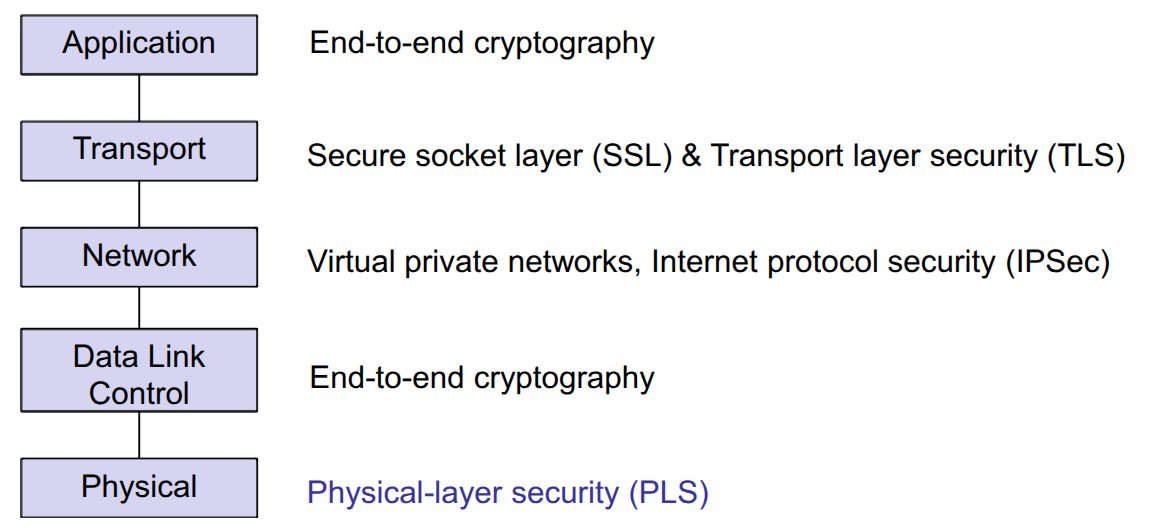
\includegraphics[width=0.8\textwidth]{chapters/figs/fig-4-1}
	\caption{مکانیزم‌های امنیتی در لایه‌های مختلف مدل \lr{OSI}. (تنها لایه‌های مرتبط با امنیت نشان داده شده‌اند)}
	\label{fig:4-1}
\end{figure}

آلیس و باب ظرفیت کانال آلیس-باب (که با نام ظرفیت کانال اصلی\LTRfootnote{Capacity of the main channel} نیز شناخته می‌شود) $C_M$ و ظرفیت محرمانگی\LTRfootnote{Secrecy capacity} $C_S$ را، که به‌صورت تفاضل بین ظرفیت کانال اصلی و ظرفیت کانال شنود\LTRfootnote{Eavesdropping channel capacity} $C_E$ تعریف می‌شود، پایش می‌کنند. زمانی که ظرفیت محرمانگی به‌میزان کافی بالاتر از مقدار آستانه $C_{S,tsh}$ و ظرفیت کانال اصلی به‌خوبی بالاتر از مقدار آستانه $C_{M,tsh}$ باشد، آلیس نمادهای با شکل گاوسی\LTRfootnote{Gaussian-shaped symbols} $X$ را برای باب ارسال می‌کند. هنگامی که هر دو ظرفیت محرمانگی و ظرفیت کانال اصلی به دلیل محوشدگی عمیق\LTRfootnote{Deep fading} پایین‌تر از آستانه‌های مربوطه قرار گیرند، آلیس و باب مصالحه اطلاعات\LTRfootnote{Information reconciliation} نمادهای ارسال‌شده قبلی را انجام می‌دهند که بر پایه طرح \lr{ECC} قوی است تا اطمینان حاصل شود که خطاهای وارد شده توسط کانال یا ایو قابل اصلاح هستند. مشابه با طرح‌های \lr{QKD} \cite{4-7, 4-8, 4-9, 4-10, 4-11, 4-12, 4-13, 4-14}، می‌توان از یک کد بررسی توازن کم‌چگال (\lr{LDPC})\LTRfootnote{Low-density parity-check (LDPC)} سیستماتیک استفاده کرد (که بر بیت‌های اطلاعات تأثیری نمی‌گذارد اما بیت‌های بررسی توازن را که به‌صورت جبری با بیت‌های اطلاعات مرتبط هستند تولید می‌کند) تا بیت‌های توازن را تولید کرده و آن‌ها را از طریق یک کانال عمومی احرازهویت‌شده ارسال نماید. طرح‌های مصالحه اطلاعات مستقیم و معکوس وجود دارند. در مصالحه مستقیم، که در شکل \ref{fig:4-2} نشان داده شده است، آلیس رمزگذاری \lr{LDPC} را انجام داده و بیت‌های توازن را برای باب ارسال می‌کند. باب رمزگشایی \lr{LDPC} را برای به‌دست آوردن کلید صحیح $X$ انجام می‌دهد. در مصالحه معکوس، باب به جای آلیس رمزگذاری \lr{LDPC} را انجام می‌دهد. سپس تقویت حریم خصوصی\LTRfootnote{Privacy amplification} بین آلیس و باب انجام می‌شود تا از $X$ مجموعه کوچک‌تری از بیت‌های $K$ (کلید امن\LTRfootnote{Secure key}) استخراج گردد که همبستگی آن با رشته ایو پایین‌تر از یک آستانه مطلوب باشد. یکی از راه‌های انجام تقویت حریم خصوصی، استفاده از توابع هش سراسری\LTRfootnote{Universal hash functions} $G$ \cite{4-9, 4-12, 4-14, 4-15} است، که مجموعه رشته‌های $n$-بیتی $X$ را به مجموعه رشته‌های $m$-بیتی $K$ نگاشت می‌کنند، به‌طوری که برای هر دو رشته متمایز $X_1$ و $X_2$ از مجموعه کلیدهای اصلاح‌شده، زمانی که نگاشت $g$ به‌صورت یکنواخت و تصادفی از $G$ انتخاب شود، احتمال برقراری $g(X_1) = g(X_2)$ بسیار پایین باشد.




\begin{figure}[ht]
	\centering
	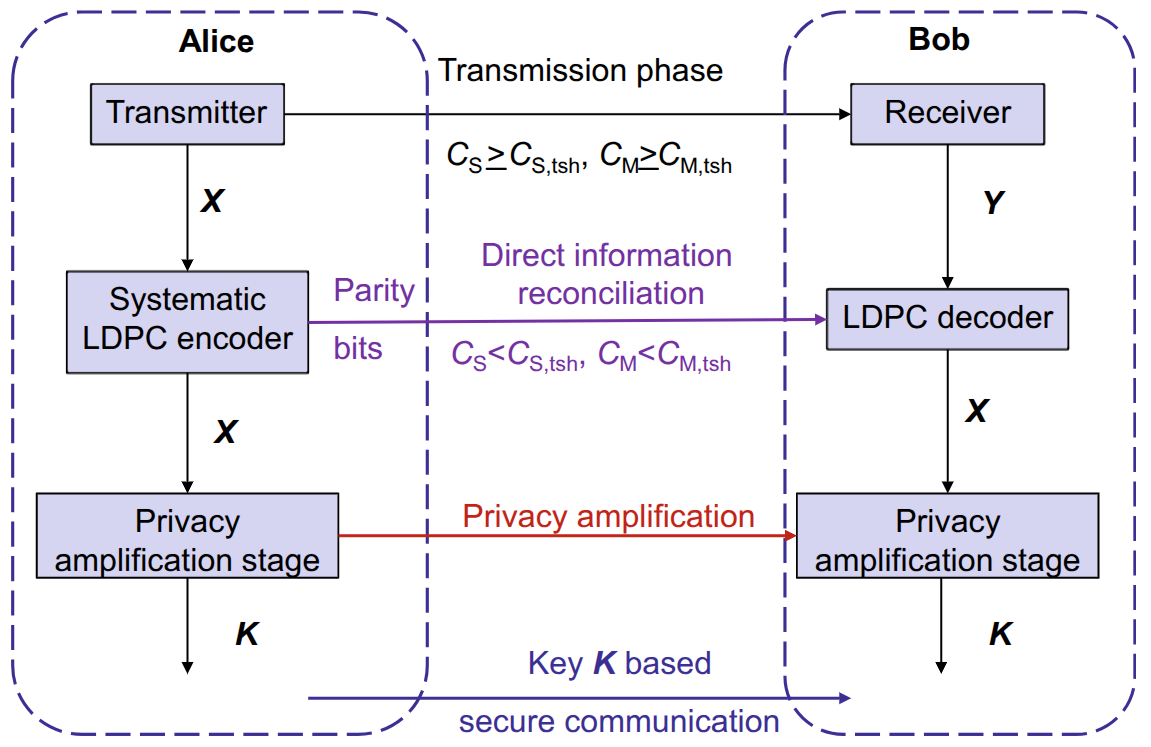
\includegraphics[width=0.8\textwidth]{chapters/figs/fig-4-2}
	\caption{پروتکل تولید (توافق) کلید مخفی مناسب برای مخابرات بی‌سیم.}
	\label{fig:4-2}
\end{figure}

\begin{figure}[ht]
	\centering
	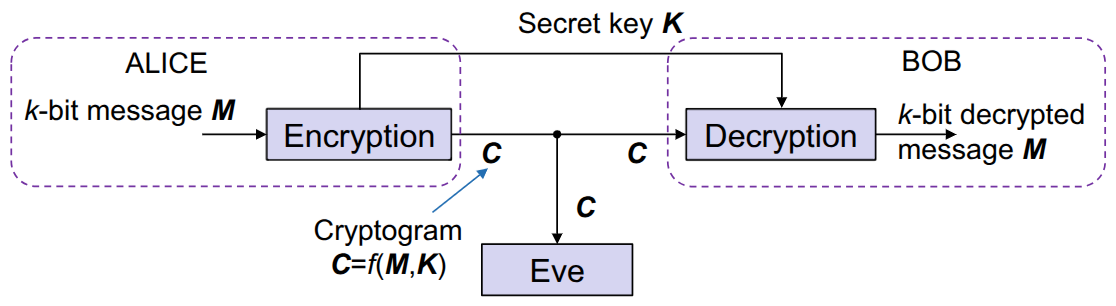
\includegraphics[width=0.8\textwidth]{chapters/figs/fig-4-3}
	\caption{مدل شانون برای سیستم محرمانگی.}
	\label{fig:4-3}
\end{figure}

\section{امنیت نظریه-اطلاعاتی در مقابل امنیت محاسباتی}
\label{sec:4-2}
مدل شانون برای سیستم محرمانگی \cite{4-16} در شکل \ref{fig:4-3} به تصویر کشیده شده است. هدف از این سیستم، ارسال قابل‌اطمینان پیام $M$ است که به‌طور هم‌زمان از دیدگاه ایو محرمانه باشد. برای انجام این کار، آلیس و باب به کلید تصادفی $K$ دسترسی دارند که برای ایو ناشناخته است و توسط آلیس برای رمزگذاری پیام به رمزنگاشت $C$ استفاده می‌شود. در سمت گیرنده، باب رمزنگاشت $C$ را با کمک کلید $K$ رمزگشایی کرده و پیام ارسالی $M$ را تعیین می‌کند.

\subsection{امنیت نظریه-اطلاعاتی (کامل)}
\label{subsec:4-2-1}
ما می‌گوییم پیام با امنیت کامل\LTRfootnote{Perfect security} ارسال شده است اگر دانش ایو درباره رمزنگاشت به او در رمزگشایی پیام کمکی نکند. به عبارت دیگر، $Pr(M | \text{Eve's knowledge}) = Pr(M)$. به‌وضوح، در مفهوم امنیت کامل، کلمه کد $C$ از نظر آماری مستقل از پیام $M$ است و می‌توانیم بنویسیم $H(M|C) = H(M)$. به‌طور معادل، اطلاعات متقابل بین کلمه کد $C$ و پیام $M$ صفر است، یعنی $I(M;C) = H(M|C) - H(M) = 0$. در این سناریو، بهترین استراتژی برای ایو حدس زدن پیام است که احتمال موفقیت آن $2^{-k}$ بوده و با افزایش طول کلید $k$ به‌صورت نمایی کاهش می‌یابد. با به‌کارگیری قاعده زنجیره‌ای\LTRfootnote{Chain rule} از فصل \ref{chap:2}، می‌توانیم بنویسیم:
\begin{equation}
	H(M) = H(M|C) \leq H(M, K|C) = H(K|C) + \underbrace{H(M|C, K)}_{0} = H(K|C) \leq H(K),
	\label{eq:4-1}
\end{equation}
که در آن از این واقعیت استفاده کردیم که وقتی هم رمزنگاشت و هم کلید معلوم باشند، پیام کاملاً مشخص می‌شود، یعنی $H(M|K, C) = 0$. بنابراین، شرط محرمانگی کامل به‌صورت زیر داده می‌شود:
\begin{equation}
	H(M) \leq H(K).
	\label{eq:4-2}
\end{equation}
در نتیجه، برای اینکه یک طرح رمزگذاری دارای امنیت کامل باشد، آنتروپی (عدم قطعیت) کلید نمی‌تواند کمتر از آنتروپی پیام باشد.
	% !TeX root = ../quantum.tex

\chapter{توزیع کلید کوانتومی}\label{chap:6}



\section{مبانی رمزنگاری}
\label{sec:6-1}


سیستم رمزنگاری\LTRfootnote{Cryptographic system} پایه مبتنی بر کلید در شکل \ref{fig:6-1} نشان داده شده است. منبع، پیام (متن‌آشکار\LTRfootnote{Plaintext}) $\bm{M}$ را به سمت بلوک رمزگذاری\LTRfootnote{Encryption} ارسال می‌کند که این بلوک با کمک کلید $\bm{K}$ دریافت شده از منبع کلید، رمزنگاشت\LTRfootnote{Cryptogram} را تولید می‌نماید. در سمت گیرنده، رمزنگاشت ارسال شده از طریق یک کانال ناامن، توسط الگوریتم رمزگشایی\LTRfootnote{Decryption} به همراه کلید $\bm{K}$ که از طریق کانال امن دریافت شده است، پردازش می‌شود که متن‌آشکار اصلی را برای تحویل به کاربر احرازهویت‌شده\LTRfootnote{Authenticated user} بازسازی می‌کند. فرآیند رمزگذاری را می‌توان به‌صورت ریاضی به‌صورت $E_{\bm{K}}(\bm{M}) = \bm{C}$ توصیف کرد، در حالی که فرآیند رمزگشایی با $D_{\bm{K}}(\bm{C}) = \bm{M}$ بیان می‌شود. ترکیب توابع رمزگشایی و رمزگذاری منجر به نگاشت همانی\LTRfootnote{Identity mapping} $D_{\bm{K}}(E_{\bm{K}}(\bm{M})) = \bm{M}$ می‌گردد. منبع کلید معمولاً کلید را به‌صورت تصادفی از فضای کلید\LTRfootnote{Keyspace} (محدوده تمام مقادیر ممکن برای کلید) تولید می‌کند.

الگوریتم‌های مبتنی بر کلید را می‌توان به دو دسته کلی تقسیم کرد:
\begin{itemize}
	\item در الگوریتم‌های متقارن\LTRfootnote{Symmetric algorithms}، کلید رمزگشایی را می‌توان از کلید رمزگذاری مشتق کرد و بالعکس. متناوباً، می‌توان از یک کلید یکسان برای هر دو مرحله رمزگذاری و رمزگشایی استفاده کرد. الگوریتم‌های متقارن با نام‌های الگوریتم‌های تک‌کلیدی\LTRfootnote{One-key (single-key) algorithms} یا کلید مخفی\LTRfootnote{Secret-key algorithms} نیز شناخته می‌شوند. یک سیستم شناخته‌شده که از این نوع الگوریتم استفاده می‌کند، استاندارد رمزگذاری دیجیتال\LTRfootnote{Digital encryption standard (DES)} است \cite{1,2,3,4}.
	\item در الگوریتم‌های نامتقارن\LTRfootnote{Asymmetric algorithms}، کلیدهای رمزگذاری و رمزگشایی متفاوت هستند. علاوه بر این، کلید رمزگشایی را نمی‌توان از روی کلید رمزگذاری تعیین کرد، حداقل نه در یک بازه زمانی معقول. به همین دلیل، کلیدهای رمزگذاری حتی می‌توانند به‌صورت عمومی منتشر شوند؛ زیرا یک شنودگر\LTRfootnote{Eavesdropper} قادر به تعیین کلید رمزگشایی نخواهد بود. سیستم‌های کلید عمومی\LTRfootnote{Public-key systems} \cite{5} بر پایه این مفهوم بنا شده‌اند. در سیستم‌های کلید عمومی، کلیدهای رمزگذاری عمومی می‌شوند، در حالی که کلید رمزگشایی تنها برای کاربر موردنظر شناخته شده است. در این حالت، کلید رمزگذاری را کلید عمومی\LTRfootnote{Public key} و کلید رمزگشایی را کلید مخفی (خصوصی)\LTRfootnote{Secret (private) key} می‌نامند. این کلیدها را می‌توان با هر ترتیبی برای ایجاد رمزنگاشت از متن‌آشکار و بازسازی متن‌آشکار از رمزنگاشت به کار برد.
\end{itemize}

\begin{figure}[h]
	\centering
	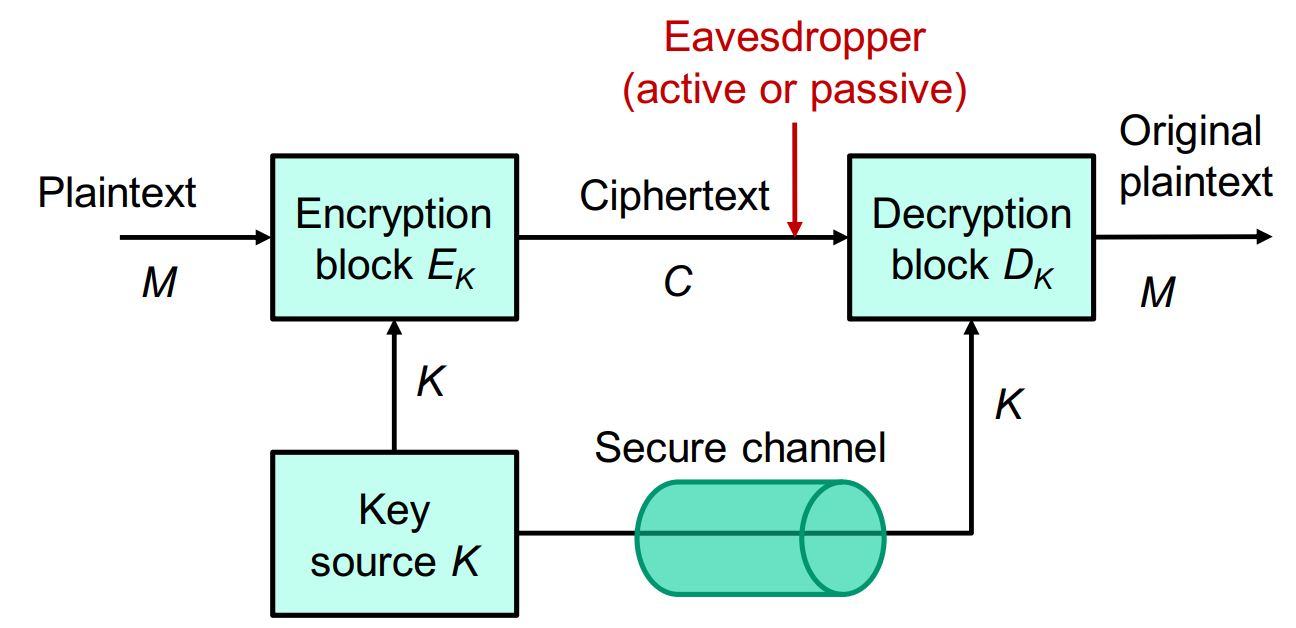
\includegraphics[width=0.7\linewidth]{chapters/figs/fig-6-1}
	\caption{طرح رمزنگاری پایه مبتنی بر کلید.}
	\label{fig:6-1}
\end{figure}

ساده‌ترین سیستم رمزنگاری کلید خصوصی، رمز ورنام\LTRfootnote{Vernam cipher} (پد یک‌بار مصرف\LTRfootnote{One-time pad}) است. در یک پد یک‌بار مصرف \cite{6}، یک دنباله کاملاً تصادفی از نویسه‌ها، با طولی برابر با طول دنباله پیام، به‌عنوان کلید استفاده می‌شود. برای هر پیام جدید، یک دنباله تصادفی دیگر به‌عنوان کلید به کار می‌رود و از این رو، طرح پد یک‌بار مصرف امنیت کامل\LTRfootnote{Perfect security} را فراهم می‌کند. به بیان دقیق‌تر، رویکرد جستجوی جامع\LTRfootnote{Brute-force search} مستلزم بررسی $m^n$ کلید احتمالی است که در آن $m$ اندازه الفبای به‌کار رفته و $n$ طول رمزنگاشتِ شنود شده است. در عمل، در ارتباطات دیجیتال و کامپیوتری، ما معمولاً در الفبای باینری $\mathrm{GF}(2) = \{0,1\}$ عمل می‌کنیم. برای به‌دست آوردن کلید، به یک مولد تصادفی خاص نیاز داریم و برای رمزگذاری با استفاده از طرح پد یک‌بار مصرف، صرفاً عمل جمع در پیمانه ۲، یعنی یک عملیات \lr{XOR}، را مطابق شکل \ref{fig:6-2} انجام می‌دهیم. طرح پد یک‌بار مصرف علی‌رغم ارائه امنیت کامل، چندین نقص دارد \cite{7,8,9}: این طرح مستلزم آن است که کلیدها به‌صورت امن توزیع شوند، طول آن‌ها حداقل به اندازه پیام باشد، بیت‌های کلید مجدداً استفاده نشوند، به‌صورت پیش‌تحویل ارائه شوند، تا زمان استفاده به‌صورت امن ذخیره گردند و پس از استفاده نابود شوند.

طبق گفته شانون \cite{10}، امنیت کامل که با نام امنیت غیرمشروط\LTRfootnote{Unconditional security} نیز شناخته می‌شود، زمانی حاصل می‌گردد که پیام‌های $\bm{M}$ و رمزنگاشت‌های $\bm{C}$ از نظر آماری مستقل باشند، به‌طوری که اطلاعات متقابل\LTRfootnote{Mutual information} متناظر با آن‌ها برابر صفر شود:
\begin{equation}
	I(\bm{M}; \bm{C}) = H(\bm{M}) - H(\bm{M}|\bm{C}) = 0 \implies H(\bm{M}|\bm{C}) = H(\bm{M})
	\label{eq:6-1}
\end{equation}
با به‌کارگیری قاعده زنجیره‌ای\LTRfootnote{Chain rule} \cite{2,11} که به‌صورت $H(X,Y) = H(X) + H(Y|X)$ بیان می‌شود، می‌توانیم بنویسیم:
\begin{equation}
	H(\bm{M}) = H(\bm{M}|\bm{C}) \leq H(\bm{M}, \bm{K}|\bm{C}) = H(\bm{K}|\bm{C}) + \underbrace{H(\bm{M}|\bm{C}, \bm{K})}_{=0} \leq H(\bm{K})
	\label{eq:6-2a}
\end{equation}
که در آن از این واقعیت استفاده شده است که وقتی هم رمزنگاشت و هم کلید معلوم باشند، پیام کاملاً مشخص می‌شود؛ یعنی $H(\bm{M}|\bm{K}, \bm{C}) = 0$. بنابراین، شرط امنیت کامل را می‌توان به‌صورت زیر خلاصه کرد:
\begin{equation}
	H(\bm{M}) \leq H(\bm{K})
	\label{eq:6-2b}
\end{equation}
به عبارت دیگر، برای اینکه یک طرح رمزگذاری دارای امنیت کامل باشد، آنتروپی\LTRfootnote{Entropy} (عدم قطعیت\LTRfootnote{Uncertainty}) کلید نمی‌تواند کمتر از آنتروپی پیام باشد. با توجه به اینکه طول کلید در رمز ورنام حداقل برابر با طول پیام است، به نظر می‌رسد طرح پد یک‌بار مصرف دارای امنیت کامل باشد.

\begin{figure}[H]
	\centering
	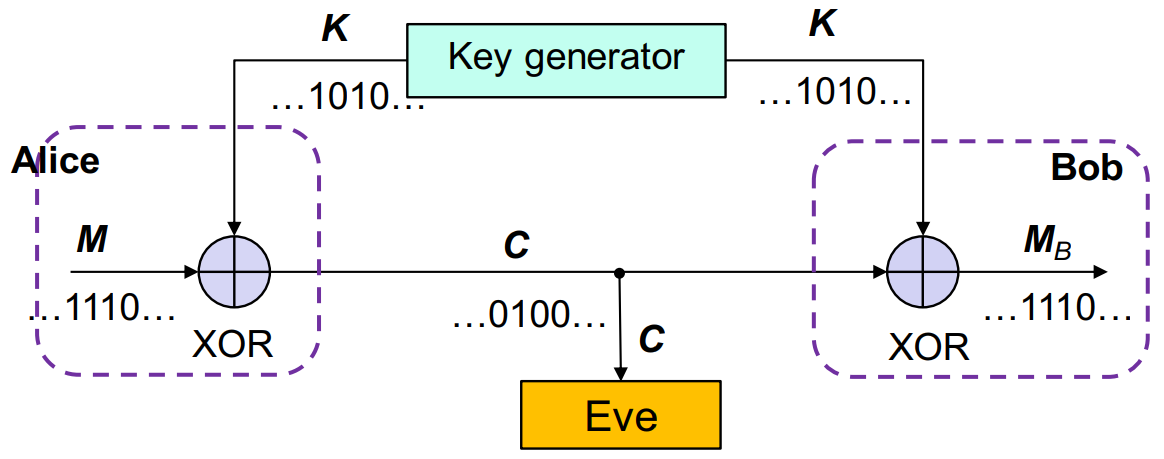
\includegraphics[width=0.7\linewidth]{chapters/figs/fig-6-2}
	\caption{طرح رمزگذاری پد یک‌بار مصرف.}
	\label{fig:6-2}
\end{figure}




\section{مبانی توزیع کلید کوانتومی}
\label{sec:6-2}

اخیراً دستاوردهای قابل‌توجهی در محاسبات کوانتومی حاصل شده است \cite{7,8,9}. بسیاری از شرکت‌ها در حال حاضر مشغول توسعه کامپیوترهای کوانتومی با مقیاس متوسط هستند. از آنجایی که اکثر سیستم‌های رمزنگاری به فرض دشواری محاسباتی\LTRfootnote{Computational hardness assumption} وابسته هستند، محاسبات کوانتومی چالشی جدی برای سیستم‌های امنیت سایبری مدرن محسوب می‌شود. به‌عنوان مثال، برای شکستن پروتکل ریواست-شامیر-ادلمن (\lr{RSA})\LTRfootnote{Rivest-Shamir-Adleman (RSA)} \cite{20}، باید دوره تناوب $r$ تابع $f(x) = m^x \pmod n = f(x+r)$ را تعیین کرد (به‌طوری که $r = 0, 1, \dots, 2^{L-1}$ و $m$ یک عدد صحیح کوچک‌تر از $n-1$ است). این دوره تناوب در یک مرحله از الگوریتم تجزیه شور \cite{7,8,9,17,18,19} تعیین می‌شود.

توزیع کلید کوانتومی (\lr{QKD}) با رمزگذاری متقارت را می‌توان به‌عنوان یک طرح امنیت لایه فیزیکی\LTRfootnote{Physical-layer security} تفسیر کرد که امنیت اثبات‌پذیری را در برابر حملات آغاز شده توسط کامپیوترهای کوانتومی فراهم می‌کند \cite{21}. اولین طرح \lr{QKD} توسط بنت\LTRfootnote{Bennett} و براسارد\LTRfootnote{Brassard} معرفی شد که آن را در سال ۱۹۸۴ پیشنهاد کردند \cite{15,16} و امروزه با نام پروتکل \lr{BB84} شناخته می‌شود. امنیت \lr{QKD} توسط قوانین مکانیک کوانتومی تضمین می‌شود. درجات آزادی فوتون\LTRfootnote{Degree-of-freedom (DOF)} (\lr{DOF}) مختلفی مانند قطبش\LTRfootnote{Polarization}، زمان، فرکانس، فاز و تکانه زاویه‌ای مداری\LTRfootnote{Orbital angular momentum} را می‌توان برای پیاده‌سازی پروتکل‌های مختلف \lr{QKD} به کار گرفت. به‌طور کلی، بسته به استراتژی اعمال شده در سمت باب\LTRfootnote{Bob}، دو طرح کلی \lr{QKD} وجود دارد: \lr{QKD} با متغیر گسسته\LTRfootnote{Discrete-variable QKD (DV-QKD)} (\lr{DV-QKD}) و \lr{QKD} با متغیر پیوسته\LTRfootnote{Continuous-variable QKD (CV-QKD)} (\lr{CV-QKD}). در طرح‌های \lr{DV-QKD}، یک آشکارساز تک‌فوتون\LTRfootnote{Single-photon detector (SPD)} (\lr{SPD}) در سمت باب به کار می‌رود، در حالی که در \lr{CV-QKD}، مولفه‌های مربعی میدان\LTRfootnote{Field quadratures} با کمک آشکارسازی هموداین/هتروداین\LTRfootnote{Homodyne/heterodyne detection} اندازه‌گیری می‌شوند. طرح \lr{DV-QKD} با به‌کارگیری قضیه کپی‌ناپذیری\LTRfootnote{No-cloning theorem} و قضیه تمایزناپذیری حالت‌های کوانتومی دلخواه\LTRfootnote{Indistinguishability of arbitrary quantum states} به امنیت غیرمشروط دست می‌یابد. قضیه کپی‌ناپذیری ادعا می‌کند که حالت‌های کوانتومی دلخواه را نمی‌توان کپی کرد، که نشان می‌دهد ایو\LTRfootnote{Eve} نمی‌تواند حالت‌های کوانتومی غیرمتعامد\LTRfootnote{Nonorthogonal} را حتی با کمک یک کامپیوتر کوانتومی بازتولید کند. از سوی دیگر، قضیه دوم بیان می‌کند که حالت‌های غیرمتعامد را نمی‌توان به‌طور ابهام‌ناپذیر متمایز کرد. به عبارت دیگر، هنگامی که ایو با حالت‌های کوانتومی ارسال‌شده تعامل برقرار می‌کند تا اطلاعاتی درباره بیت‌های ارسالی به‌دست آورد، به‌طور ناخواسته وفاداری\LTRfootnote{Fidelity} حالت‌های کوانتومی را مختل می‌کند که باب آن را آشکار خواهد کرد. از طرف دیگر، \lr{CV-QKD} از اصل عدم قطعیت\LTRfootnote{Uncertainty principle} بهره می‌برد که بیان می‌کند هر دو مولفه هم‌فاز\LTRfootnote{In-phase} و مربعی\LTRfootnote{Quadrature} حالت‌های همدوس\LTRfootnote{Coherent states} را نمی‌توان به‌طور هم‌زمان با دقت کامل اندازه‌گیری کرد. ما همچنین می‌توانیم طرح‌های مختلف \lr{QKD} را به دو نوع «به کمک درهم‌تنیدگی»\LTRfootnote{Entanglement-assisted} یا «آماده‌سازی-و-اندازه‌گیری»\LTRfootnote{Prepare-and-measure} طبقه‌بندی کنیم.

\begin{figure}[H]
	\centering
	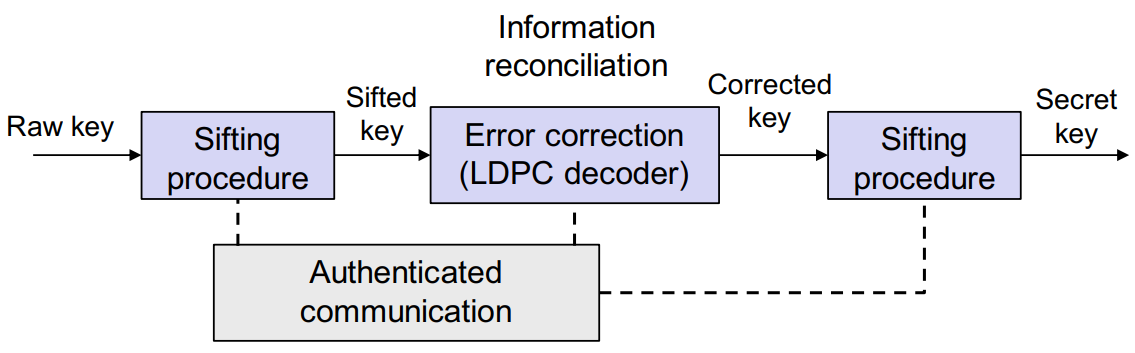
\includegraphics[width=0.9\linewidth]{chapters/figs/fig-6-3}
	\caption{مراحل پس‌پردازش کلاسیک.}
	\label{fig:6-3}
\end{figure}

مصالحه اطلاعات چیزی جز تصحیح خطا نیست که بر روی یک کانال عمومی\LTRfootnote{Public channel} انجام می‌شود و خطاها را بین $\bm{X}$ و $\bm{Y}$ مصالحه می‌کند تا یک رشته بیت مشترک $\bm{K}$ به‌دست آید، در حالی که اطلاعات فاش‌شده برای ایو تا حد امکان کمینه باشد.

تقویت حریم خصوصی\LTRfootnote{Privacy amplification} \cite{23, 24} بین آلیس و باب برای استخراج\LTRfootnote{Distill} مجموعه کوچکتری از بیت‌ها $\bm{S}$ از $\bm{K}$ استفاده می‌شود که همبستگی آن با رشته ایو $\bm{Z}$ زیر آستانه مطلوب باشد. یکی از راه‌های انجام تقویت حریم خصوصی، استفاده از توابع هش سراسری\LTRfootnote{Universal hash functions} $G$ است که مجموعه رشته‌های $n$-بیتی $A$ را به مجموعه رشته‌های $m$-بیتی $B$ نگاشت می‌کنند، به‌طوری که برای هر دو رشته متمایز $a_1, a_2 \in A$، وقتی $g$ به‌صورت یکنواخت و تصادفی از $G$ انتخاب شود، احتمال برقراری $g(a_1) = g(a_2)$ حداکثر $1/|B|$ باشد.

جزئیات بیشتر در مورد مصالحه اطلاعات و تقویت حریم خصوصی در بخش \ref{sec:6-9} از این فصل ارائه خواهد شد.





\section{قضیه کپی‌ناپذیری و تمایز حالت‌های کوانتومی}
\label{sec:6-3}

\begin{theorem}
	\label{thm:6-1}
	\textbf{(قضیه کپی‌ناپذیری\LTRfootnote{No-cloning theorem})}
	هیچ کپی‌کننده کوانتومی وجود ندارد که بتواند یک حالت کوانتومی دلخواه را کپی کند.
\end{theorem}

\begin{proof}
	اگر حالت ورودی $|\psi\rangle$ باشد، خروجی کپی‌کننده باید به صورت $|\psi\rangle|\psi\rangle$ باشد. برای یک حالت کوانتومی دلخواه، وجود چنین کپی‌کننده‌ای منجر به یک تناقض بنیادی می‌شود. دو حالت دلخواه $|\psi\rangle$ و $|\phi\rangle$ را در نظر بگیرید که به عنوان ورودی به کپی‌کننده داده می‌شوند. وقتی این حالت‌ها به صورت مجزا وارد شوند، انتظار داریم خروجی‌های $|\psi\rangle|\psi\rangle$ و $|\phi\rangle|\phi\rangle$ را به‌دست آوریم. اکنون برهم‌نهی\LTRfootnote{Superposition} این دو حالت را به صورت زیر در نظر بگیرید:
	\begin{equation}
		\begin{aligned}
			|\Psi\rangle = a|\psi\rangle + b|\phi\rangle \implies |\Psi\rangle|\Psi\rangle &= (a|\psi\rangle + b|\phi\rangle)(a|\psi\rangle + b|\phi\rangle) \\ &= a^2|\psi\rangle|\psi\rangle + ab|\psi\rangle|\phi\rangle + ab|\phi\rangle|\psi\rangle + b^2|\phi\rangle|\phi\rangle
		\end{aligned}
		\label{eq:6-3}
	\end{equation}
	از سوی دیگر، خطی بودن مکانیک کوانتومی به ما می‌گوید که کپی‌کننده کوانتومی را می‌توان با یک عملگر یکانی\LTRfootnote{Unitary operator} بازنمایی کرد که عمل کپی کردن را انجام می‌دهد. اگر چنین عملگر یکانی بر روی حالت برهم‌نهی $|\Psi\rangle$ اثر کند، خروجی باید برهم‌نهی از $|\psi\rangle|\psi\rangle$ و $|\phi\rangle|\phi\rangle$ باشد؛ یعنی:
	\begin{equation}
		|\Psi'\rangle = a|\psi\rangle|\psi\rangle + b|\phi\rangle|\phi\rangle
		\label{eq:6-4}
	\end{equation}
	تفاوت بین دو معادله \eqref{eq:6-3} و \eqref{eq:6-4} منجر به تناقض ذکر شده در بالا می‌شود. در نتیجه، هیچ عملگر یکانی وجود ندارد که بتواند $|\Psi\rangle$ را کپی کند.
\end{proof}

این نتیجه پرسش مرتبطی را ایجاد می‌کند: آیا حالت‌های خاصی وجود دارند که کپی کردن آن‌ها امکان‌پذیر باشد؟ پاسخ به این پرسش (به‌طور شگفت‌انگیزی) مثبت است؛ کپی کردن تنها برای حالت‌های متعامد متقابل امکان‌پذیر است.

\begin{theorem}
	\label{thm:6-2}
	تمایز ابهام‌ناپذیر حالت‌های کوانتومی غیرمتعامد غیرممکن است.
	
	
	به عبارت دیگر، هیچ دستگاه اندازه‌گیری نمی‌توان ساخت که بتواند با اطمینان حالت‌های غیرمتعامد را متمایز کند. این نتیجه بنیادی نقش مهمی در رمزنگاری کوانتومی ایفا می‌کند.
\end{theorem}

\begin{proof}
	اثبات این قضیه بر پایه تناقض\LTRfootnote{Contradiction} است. فرض کنید عملگر اندازه‌گیری $M$ یک عملگر هرمیتی\LTRfootnote{Hermitian operator} با مقادیر ویژه\LTRfootnote{Eigenvalues} $m_i$ و عملگرهای تصویر\LTRfootnote{Projection operators} $P_i$ متناظر باشد که به ما اجازه می‌دهد به‌طور ابهام‌ناپذیر بین دو حالت غیرمتعامد $|\psi_1\rangle$ و $|\psi_2\rangle$ تمایز قائل شویم. مقدار ویژه $m_1$ ($m_2$) به‌طور ابهام‌ناپذیر حالت $|\psi_1\rangle$ ($|\psi_2\rangle$) را شناسایی می‌کند. می‌دانیم که برای عملگرهای تصویر، ویژگی‌های زیر برقرار است:
	\begin{equation}
		\langle\psi_1|P_1|\psi_1\rangle = 1; \quad \langle\psi_2|P_2|\psi_2\rangle = 1; \quad \langle\psi_1|P_2|\psi_1\rangle = 0; \quad \langle\psi_2|P_1|\psi_2\rangle = 0
		\label{eq:6-5}
	\end{equation}
	با توجه به موارد فوق، $|\psi_2\rangle$ را می‌توان برحسب $|\psi_1\rangle$ و حالت دیگری مانند $|\phi\rangle$ که بر $|\psi_1\rangle$ متعامد است، به صورت زیر نمایش داد:
	\begin{equation}
		|\psi_2\rangle = a|\psi_1\rangle + b|\phi\rangle
		\label{eq:6-6}
	\end{equation}
	برای برقراری رابطه \eqref{eq:6-5}، $|\psi_2\rangle$ باید با $|\phi\rangle$ برابر باشد (یعنی $a=0$)، که این امر نشان‌دهنده یک تناقض است (زیرا فرض شده بود دو حالت غیرمتعامد هستند).
\end{proof}





\section{پروتکل‌های توزیع کلید کوانتومی با متغیر گسسته}
\label{sec:6-4}

در این بخش، برخی از پروتکل‌های مرتبط با \lr{DV-QKD} از جمله \lr{BB84}، \lr{B92}، کدگذاری فاز-زمان\LTRfootnote{Time-phase encoding}، \lr{E91} و پروتکل‌های اینشتین-پودولسکی-روزن (\lr{EPR})\LTRfootnote{Einstein-Podolsky-Rosen (EPR)} را شرح می‌دهیم.

\subsection{پروتکل‌های \lr{BB84}}
\label{subsec:6-4-1}

پروتکل \lr{BB84} به نام بنت\LTRfootnote{Bennett} و براسارد\LTRfootnote{Brassard} نام‌گذاری شده است که آن را در سال ۱۹۸۴ پیشنهاد کردند \cite{15,16}. سه اصل کلیدی به‌کار گرفته شده در این پروتکل عبارتند از: قضیه کپی‌ناپذیری، فروپاشی حالت\LTRfootnote{State collapse} در طول اندازه‌گیری، و بازگشت‌ناپذیری اندازه‌گیری‌ها\LTRfootnote{Irreversibility of measurements} \cite{7}. پروتکل \lr{BB84} را می‌توان با استفاده از درجات آزادی مختلف، از جمله درجه آزادی قطبش\LTRfootnote{Polarization} \cite{25} یا فاز فوتون‌ها \cite{22} پیاده‌سازی کرد. از نظر تجربی، پروتکل \lr{BB84} در هر دو کانال فیبر نوری و نوری فضای آزاد (\lr{FSO})\LTRfootnote{Free-space-optical (FSO)} نمایش داده شده است \cite{25,26}. پروتکل \lr{BB84} مبتنی بر قطبش در کانال‌های فیبر نوری تحت تأثیر پاشندگی مد قطبشی\LTRfootnote{Polarization mode dispersion}، تلفات وابسته به قطبش\LTRfootnote{Polarization-dependent loss} و تلفات فیبر قرار می‌گیرد که مسافت ارسال را محدود می‌کنند. برای افزایش مسافت ارسال، از کدگذاری فاز استفاده می‌شود، مانند آنچه در مرجع \cite{26} آمده است. متأسفانه نرخ کلید امن در ۴۰۵ کیلومتر فیبر با تلفات بسیار کم، بسیار ناچیز و تنها برابر با $6.5$ بیت بر ثانیه است. در یک کانال \lr{FSO}، اثرات قطبش به حداقل می‌رسد؛ با این حال، تلاطم اتمسفری\LTRfootnote{Atmospheric turbulence} می‌تواند منجر به اعوجاج جبهه‌موج\LTRfootnote{Wavefront distortion} و نوسانات فاز تصادفی شود. نمایش‌های قبلی \lr{QKD} شامل پیوند \lr{FSO} ماهواره به زمین و پیوند \lr{FSO} بین دو نقطه در جزایر قناری بوده است \cite{25}.

دو پایه‌ای که در پروتکل \lr{BB84} استفاده می‌شوند، پایه محاسباتی\LTRfootnote{Computational basis} $CB = \{|0\rangle, |1\rangle\}$ و پایه قطری\LTRfootnote{Diagonal basis} هستند:
\begin{equation}
	DB = \left\{ |+\rangle = \frac{|0\rangle + |1\rangle}{\sqrt{2}} ; \quad |-\rangle = \frac{|0\rangle - |1\rangle}{\sqrt{2}} \right\}
	\label{eq:6-7}
\end{equation}
این پایه‌ها به دسته‌ای از پایه‌های متقابلاً بدون سوگیری\LTRfootnote{Mutually unbiased bases (MUBs)} (\lr{MUBs}) تعلق دارند \cite{27,28,29,30,31}. دو پایه متعامد\LTRfootnote{Orthonormal bases} $\{|e_1\rangle, \dots, |e_N\rangle\}$ و $\{|f_1\rangle, \dots, |f_N\rangle\}$ در فضای هیلبرت $\mathbb{C}^N$ زمانی \lr{MUB} هستند که مجذور اندازه ضرب داخلی بین هر دو حالت پایه $\{|e_m\rangle\}$ و $\{|f_n\rangle\}$ برابر با معکوس بعد باشد:
\begin{equation}
	|\langle e_m | f_n \rangle|^2 = \frac{1}{N} \quad m, n \in \{1, \dots, N\}
	\label{eq:6-8}
\end{equation}
واژه کلیدی «بدون سوگیری»\LTRfootnote{Unbiased} بدین معناست که اگر سیستمی در حالتی متعلق به یکی از پایه‌ها آماده‌سازی شود، تمام نتایج اندازه‌گیری نسبت به پایه‌های دیگر به یک اندازه محتمل هستند.

آلیس به‌طور تصادفی یک \lr{MUB} و به دنبال آن به‌طور تصادفی یک حالت پایه را انتخاب می‌کند. مقدار منطقی $0$ توسط حالت‌های $|0\rangle$ و $|+\rangle$، و مقدار منطقی $1$ توسط $|1\rangle$ و $|-\rangle$ بازنمایی می‌شود. باب هر کیوبیت را با انتخاب تصادفی پایه (محاسباتی یا قطری) اندازه‌گیری می‌کند. در یک فرآیند غربال‌گری\LTRfootnote{Sifting procedure}، آلیس و باب پایه‌های استفاده شده برای هر کیوبیت را اعلام کرده و تنها مواردی را نگه می‌دارند که در آن‌ها از پایه یکسانی استفاده شده است.

اکنون پروتکل \lr{QKD} مبتنی بر قطبش \lr{BB84} را با چهار حالت متناظر به‌کار رفته، مطابق شکل \ref{fig:6-4} شرح می‌دهیم. پیاده‌سازی با قطعات اپتیکی حجیم\LTRfootnote{Bulky optics} برای پروتکل \lr{BB84} در شکل \ref{fig:6-5} تصویر شده است.

حالت خروجی لیزر با عنوان حالت همدوس\LTRfootnote{Coherent state} شناخته می‌شود \cite{31,32,33,34,35,36} که نشان‌دهنده کِت ویژه راست عملگر نابودی\LTRfootnote{Annihilation operator} $a$ است؛ یعنی $a|\alpha\rangle = \alpha|\alpha\rangle$ که در آن $\alpha$ مقدار ویژه مختلط است. بردار حالت همدوس $|\alpha\rangle$ را می‌توان برحسب کِت‌های ویژه متعامد $|n\rangle$ (حالت تعداد یا حالت فوک\LTRfootnote{Fock state}) عملگر تعداد $N = a^\dagger a$ به‌صورت زیر نشان داد:
\begin{equation}
	|\alpha\rangle = \exp\big(-\frac{|\alpha|^2}{2}\big) \sum_{n=0}^{\infty} \frac{\alpha^n}{\sqrt{n!}} |n\rangle
	\label{eq:6-9}
\end{equation}

\begin{figure}[H]
	\centering
	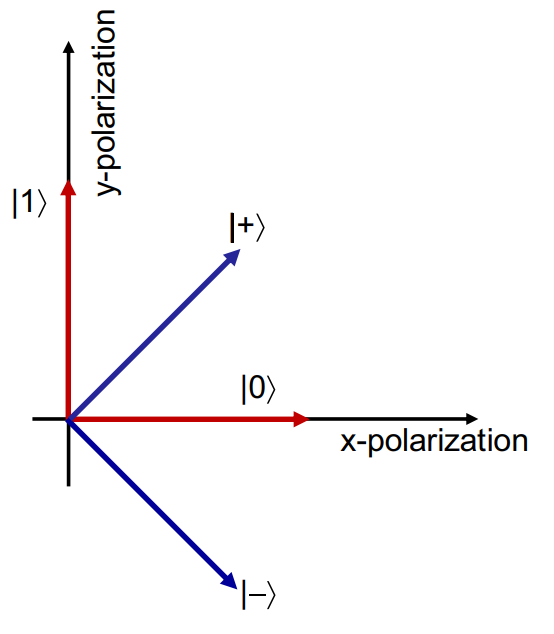
\includegraphics[width=0.5\linewidth]{chapters/figs/fig-6-4}
	\caption{چهار حالت به‌کار رفته در پروتکل \lr{BB84}.}
	\label{fig:6-4}
\end{figure}


حالت‌های همدوس متعامد نیستند، زیرا رابطه زیر برقرار است:
\begin{equation}
	\begin{aligned}
		|\langle\alpha | \beta\rangle|^2 &= \left| e^{-(|\alpha|^2+|\beta|^2)/2} \sum_{n=0}^{+\infty} \sum_{m=0}^{+\infty} (n!)^{-1/2}(m!)^{-1/2} \alpha^n (\beta^*)^m \langle n|m\rangle \right|^2 \\
		&= \left| e^{-(|\alpha|^2+|\beta|^2)/2} \sum_{n=0}^{+\infty} (n!)^{-1} \alpha^n (\beta^*)^n \right|^2 = \left| e^{-(|\alpha|^2+|\beta|^2-2\alpha\beta^*)/2} \right|^2 = e^{-|\alpha-\beta|^2}
	\end{aligned}
	\label{eq:6-10}
\end{equation}
با تضعیف کافی حالت همدوس، به حالت همدوس ضعیف\LTRfootnote{Weak coherent state (WCS)} (\lr{WCS}) دست می‌یابیم که در آن احتمال تولید بیش از یک فوتون بسیار کم است. برای مثال، به ازای $\alpha = 0.1$ خواهیم داشت:
$|0.1\rangle = \sqrt{0.90} |0\rangle + \sqrt{0.09} |1\rangle + \sqrt{0.002} |2\rangle + \dots$.
حالت تعداد $|n\rangle$ را می‌توان برحسب حالت پایه\LTRfootnote{Ground state} ($|0\rangle$) و با کمک عملگر تولید\LTRfootnote{Creation operator} به‌صورت زیر بیان کرد:


\begin{figure}[H]
	\centering
	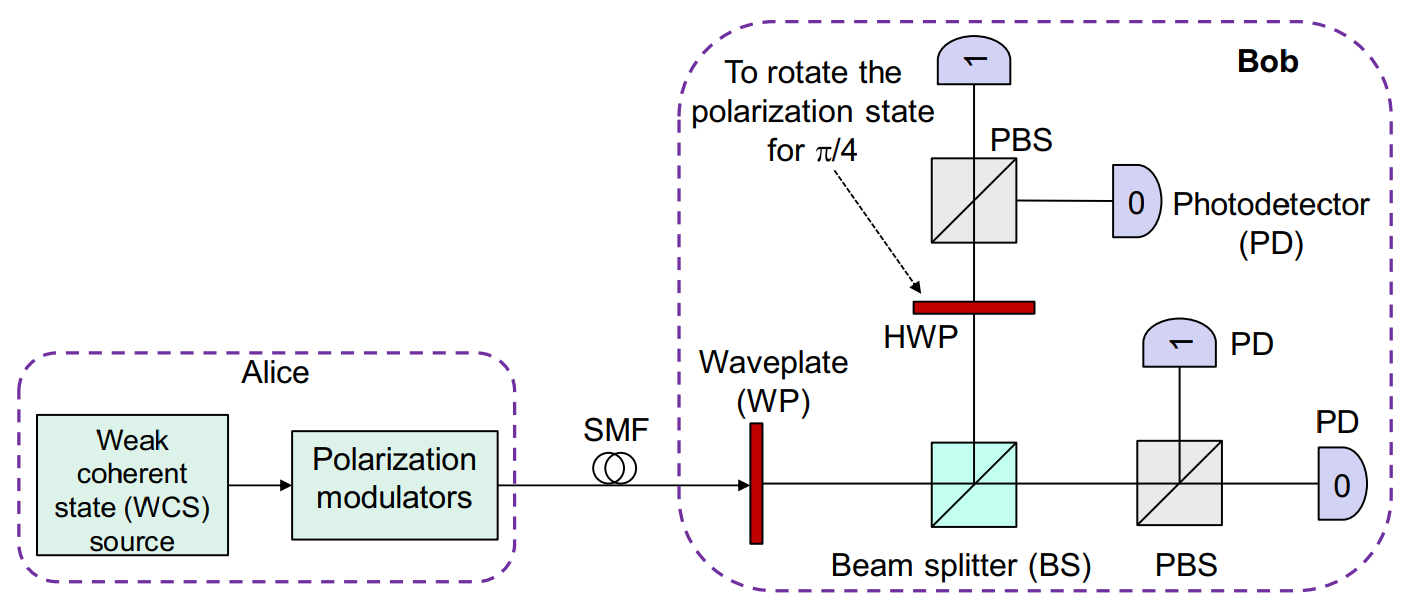
\includegraphics[width=\linewidth]{chapters/figs/fig-6-5}
	\caption{پروتکل \lr{BB84} مبتنی بر قطبش.}
	\label{fig:6-5}
\end{figure}




\begin{equation}
	|n\rangle = \frac{(a^\dagger)^n}{(n!)^{1/2}} |0\rangle 
	\label{eq:6-11}
\end{equation}
عملگر چگالی\LTRfootnote{Density operator} یک حالت همدوس به‌صورت زیر داده می‌شود:
\begin{equation}
	\rho = |\alpha\rangle\langle\alpha| = e^{-|\alpha|^2} \sum_{n=0}^{+\infty} \sum_{m=0}^{+\infty} \frac{\alpha^n (\alpha^*)^m}{(n!)^{1/2}(m!)^{1/2}} |n\rangle\langle m| 
	\label{eq:6-12}
\end{equation}
جملات قطری $\rho$ به‌صورت زیر تعیین می‌شوند:
\begin{equation}
	\langle n|\rho|n\rangle = e^{-|\alpha|^2} \frac{|\alpha|^{2n}}{n!} 
	\label{eq:6-13}
\end{equation}
که آشکارا یک توزیع پواسون\LTRfootnote{Poisson distribution} برای میانگین تعداد فوتون‌های $|\alpha|^2$ است. بنابراین، احتمال اینکه $n$ فوتون در یک حالت همدوس $|\alpha\rangle$ یافت شود، از توزیع پواسون پیروی می‌کند:
\begin{equation}
	P(n) = |\langle n|\alpha\rangle|^2 = \frac{e^{-\mu} \mu^n}{n!}
	\label{eq:6-14}
\end{equation}
که در آن از $\mu = |\alpha|^2$ برای نشان دادن میانگین تعداد فوتون‌ها استفاده می‌کنیم.

با توجه به اینکه اکنون احتمال ارسال چندین فوتون غیرصفر است، ایو می‌تواند از این واقعیت برای کسب اطلاعات از کانال بهره‌برداری کند که این کار با عنوان حمله تقسیم تعداد فوتون\LTRfootnote{Photon number splitting (PNS) attack} (\lr{PNS}) شناخته می‌شود. با فرض اینکه او بتواند تعداد فوتون‌هایی را که به او می‌رسد بدون انجام اندازه‌گیری روی سیستم تشخیص دهد، زمانی که چندین فوتون شناسایی شوند، ایو یک تک‌فوتون را برداشته و آن را در حافظه کوانتومی\LTRfootnote{Quantum memory} قرار می‌دهد تا زمانی که آلیس و باب غربال‌گری زمانی و مصالحه پایه‌ها را انجام دهند. با یادگیری پایه‌های اندازه‌گیری آلیس و باب از طریق بحث در کانال عمومی احرازهویت‌شده، فوتون‌های ذخیره‌شده در حافظه کوانتومی در پایه صحیح اندازه‌گیری می‌شوند و تمام اطلاعات موجود در فوتون را در اختیار ایو قرار می‌دهند.

برای غلبه بر حمله \lr{PNS}، استفاده از \lr{QKD} مبتنی بر حالت فریب\LTRfootnote{Decoy-state} در مرجع \cite{37} پیشنهاد شد. در \lr{QKD} حالت فریب، میانگین تعداد فوتون‌های ارسالی در بازه‌های زمانی تصادفی افزایش می‌یابد که به آلیس و باب اجازه می‌دهد تشخیص دهند که آیا در زمان ارسال چندین فوتون، ایو در حال سرقت فوتون‌ها است یا خیر.







\subsection{پروتکل B92}
\label{subsec:6-4-2}

پروتکل \lr{B92} که در سال $1992$ توسط بنت\LTRfootnote{Bennett} معرفی شد \cite{38}، تنها از دو حالت غیرمتعامد استفاده می‌کند که در شکل \ref{fig:6-6} نشان داده شده است. آلیس به‌طور تصادفی یک بیت کلاسیک $d$ تولید می‌کند و بسته به مقدار آن ($0$ یا $1$)، حالت زیر را برای باب ارسال می‌نماید \cite{7}:



\begin{figure}[ht]
	\centering
	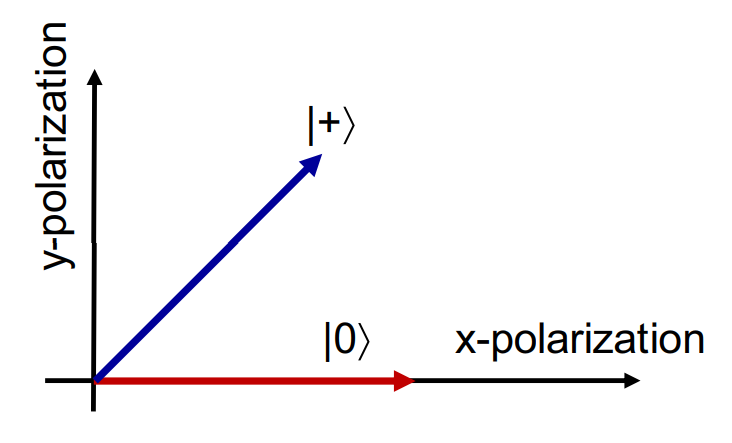
\includegraphics[width=0.6\textwidth]{chapters/figs/fig-6-6}
	\caption{دو حالت به‌کار رفته در پروتکل \lr{B92}.}
	\label{fig:6-6}
\end{figure}

\begin{equation}
	|\psi\rangle = 
	\begin{cases} 
		|0\rangle, & d = 0 \\ 
		|+\rangle = (|0\rangle + |1\rangle)/\sqrt{2}, & d = 1 
	\end{cases}
	\label{eq:6-15}
\end{equation}

باب به‌طور تصادفی یک بیت کلاسیک $d'$ تولید کرده و متعاقباً کیوبیت‌های دریافتی را در پایه $CB = \{|0\rangle, |1\rangle\}$ (اگر $d'=0$) یا در پایه $DB = \{|+\rangle, |-\rangle\}$ (اگر $d'=1$) اندازه‌گیری می‌کند؛ به‌طوری که نتیجه اندازه‌گیری $r=0$ یا $1$ متناظر با حالت‌های ویژه\LTRfootnote{Eigenstates} $1$ و $1+$ از مشاهده‌پذیرهای\LTRfootnote{Observables} $Z$ و $X$ است، همان‌طور که در جدول \ref{tab:6-1} نشان داده شده است. به‌وضوح، هنگامی که نتیجه اندازه‌گیری $r=0$ باشد، حالت‌های احتمالی ارسال شده توسط آلیس $|0\rangle$ و $|+\rangle$ هستند و باب نمی‌داند آلیس کدام حالت را ارسال کرده است. از سوی دیگر، وقتی نتیجه اندازه‌گیری $r=1$ باشد، حالت‌های احتمالی آشکار شده توسط باب $|1\rangle$ و $|-\rangle$ هستند و بیت آشکار شده توسط باب متمم بیت آلیس است. باب به‌صورت عمومی مقدار $r$ را اعلام می‌کند (و البته $d'$ را مخفی نگه می‌دارد). آلیس و باب تنها آن جفت‌های $\{d, d'\}$ را نگه می‌دارند که برای آن‌ها نتیجه اندازه‌گیری $r=1$ بوده است. بیت نهایی کلید برای آلیس $d$ و برای باب $1-d'$ است. پس از آن، مراحل مصالحه اطلاعات و تقویت حریم خصوصی انجام می‌شوند.




\subsection{پروتکل‌های اکرت (\lr{E91}) و اینشتین-پودولسکی-روزن}
\label{subsec:6-4-3}

پروتکل اکرت (\lr{E91})\LTRfootnote{Ekert (E91) protocol} توسط اکرت در سال ۱۹۹۱ معرفی شد \cite{39} (همچنین ببینید \cite{7}). فرض کنید آلیس و باب $n$ جفت کیوبیت درهم‌تنیده\LTRfootnote{Entangled pairs} در حالت بل\LTRfootnote{Bell state} (جفت \lr{EPR}\LTRfootnote{Einstein-Podolsky-Rosen (EPR)}) $|B_{00}\rangle$ به اشتراک می‌گذارند:
\begin{equation}
	|B_{00}\rangle = \frac{|00\rangle + |11\rangle}{\sqrt{2}}
	\label{eq:6-16}
\end{equation}
آلیس یک بیت کلاسیک تصادفی $\bm{b}$ را برای تعیین پایه تولید کرده و نیمه خود از حالت بل را یا در پایه محاسباتی (\lr{CB}) برای $\bm{b}=0$ یا پایه قطری (\lr{DB}) برای $\bm{b}=1$ اندازه‌گیری می‌کند تا بیت داده $\bm{d}$ را به‌دست آورد. از سوی دیگر و به شکلی مشابه، باب بیت پایه $\bm{b'}$ را به‌طور تصادفی تولید کرده و یا در پایه \lr{CB} یا \lr{DB} اندازه‌گیری انجام می‌دهد تا $\bm{d'}$ را به‌دست آورد. آلیس و باب پایه‌های استفاده‌شده، یعنی $\bm{b}$ و $\bm{b'}$ را با هم مقایسه کرده و تنها آن مواردی از $\{\bm{d}, \bm{d'}\}$ را برای کلید خام خود نگه می‌دارند که در آن‌ها پایه‌ها یکسان بوده است ($\bm{b} = \bm{b'}$). واضح است که کلید خام تولید شده کاملاً تصادفی است؛ این کلید تا زمانی که آلیس و باب اندازه‌گیری را روی نیمه‌های خود از حالت بل انجام ندهند، نامعین باقی می‌ماند. به همین دلیل، \lr{QKD} اساساً یک روش تولید کلید مخفی\LTRfootnote{Secret key generation method} است که توسط منبع درهم‌تنیده تعیین می‌شود. اگر به جای آن، از حالت بل $|B_{01}\rangle = (|01\rangle + |10\rangle)/\sqrt{2}$ استفاده می‌شد، دنباله کلید خام باب متمم دنباله کلید خام آلیس می‌بود.



\begin{table}[ht]
	\centering
	\caption{توضیح پروتکل \lr{B92}.}
	\label{tab:6-1}
	\footnotesize
	\renewcommand{\arraystretch}{1.8} % تنظیم فاصله ردیف‌ها برای خوانایی بهتر
	\begin{tabular}{|p{4.5cm} | l | l | l | l |}
		\hline
		\rowcolor{tablezebra}
		بیت‌های تولید شده توسط آلیس & \multicolumn{2}{l|}{$d = 0$} & \multicolumn{2}{l|}{$d = 1$} \\
		حالت‌های ارسال شده توسط آلیس & \multicolumn{2}{l|}{$|0\rangle$} & \multicolumn{2}{l|}{$|+\rangle$} \\
		\rowcolor{tablezebra}
		بیت‌های تولید شده توسط باب & $d' = 0$ & \multicolumn{1}{l|}{$d' = 1$} & $d' = 0$ & \multicolumn{1}{l|}{$d' = 1$} \\
		پایه اندازه‌گیری باب & 
		$\text{\lr{CB}}: \{|0\rangle, |1\rangle\}$ & \multicolumn{1}{l|}{$\text{\lr{DB}}: \{|+\rangle, |-\rangle\}$} & $\text{\lr{CB}}: \{|0\rangle, |1\rangle\}$ & \multicolumn{1}{l|}{$\text{\lr{DB}}: \{|+\rangle, |-\rangle\}$} \\
		\rowcolor{tablezebra}
		 حالت‌های حاصل احتمالی برای آشکارسازی توسط باب & $|0\rangle \quad |1\rangle$ & \multicolumn{1}{l|}{$|+\rangle \quad |-\rangle$} & $|0\rangle \quad |1\rangle$ & \multicolumn{1}{l|}{$|+\rangle \quad |-\rangle$} \\
		احتمال اندازه‌گیری یک حالت معین توسط باب & $1 \quad\; 0$ & \multicolumn{1}{l|}{$1/2 \quad 1/2$} & $1/2 \quad 1/2$ & \multicolumn{1}{l|}{$1 \quad\; 0$} \\
		\rowcolor{tablezebra}
		نتیجه اندازه‌گیری باب $r$ & $0 \quad\; -$ & \multicolumn{1}{l|}{$0 \quad\; 1$} & $0 \quad\; 1$ & \multicolumn{1}{l|}{$0 \quad\; -$} \\
		\hline
	\end{tabular}
\end{table}



پروتکل \lr{EPR} یک پروتکل سه‌حالتی است که از نامساوی بل\LTRfootnote{Bell's inequality} برای تشخیص حضور ایو به عنوان یک متغیر تصادفی پنهان\LTRfootnote{Hidden random variable} استفاده می‌کند، همان‌طور که در مرجع \cite{40} توصیف شده است. فرض کنید $|\theta\rangle$ نشان‌دهنده حالت قطبش\LTRfootnote{Polarization state} فوتونی باشد که به صورت خطی در زاویه $\theta$ قطبیده شده است. سه حالت قطبش ممکن برای جفت \lr{EPR} عبارتند از \cite{40}:
\begin{equation}
	|B_0\rangle = \frac{|0\rangle|3\pi/6\rangle + |3\pi/6\rangle|0\rangle}{\sqrt{2}}; \quad |B_1\rangle = \frac{|\pi/6\rangle|4\pi/6\rangle + |4\pi/6\rangle|\pi/6\rangle}{\sqrt{2}}; \quad |B_2\rangle = \frac{|2\pi/6\rangle|5\pi/6\rangle + |5\pi/6\rangle|2\pi/6\rangle}{\sqrt{2}}
	\label{eq:6-17}
\end{equation}
برای هر جفت \lr{EPR}، قواعد کدگذاری\LTRfootnote{Encoding rules} زیر را اعمال می‌کنیم \cite{40}:
\begin{equation}
	|\psi\rangle_1 = \begin{cases} |0\rangle, & \bm{d} = 0 \\ |3\pi/6\rangle, & \bm{d} = 1 \end{cases}; \quad |\psi\rangle_2 = \begin{cases} |\pi/6\rangle, & \bm{d} = 0 \\ |4\pi/6\rangle, & \bm{d} = 1 \end{cases}; \quad |\psi\rangle_3 = \begin{cases} |2\pi/6\rangle, & \bm{d} = 0 \\ |5\pi/6\rangle, & \bm{d} = 1 \end{cases}
	\label{eq:6-18}
\end{equation}
عملگرهای اندازه‌گیری\LTRfootnote{Measurement operators} متناظر نیز به‌صورت زیر خواهند بود \cite{40}:
\begin{equation}
	M_0 = |0\rangle\langle 0|; \quad M_1 = |\pi/6\rangle\langle \pi/6|; \quad M_2 = |2\pi/6\rangle\langle 2\pi/6|
	\label{eq:6-19}
\end{equation}

پروتکل \lr{EPR} را می‌توان به شرح زیر توصیف کرد. حالت \lr{EPR} یعنی $|B_i\rangle$ ($i = 0, 1, 2$) به‌طور تصادفی انتخاب می‌شود. فوتون اول در جفت \lr{EPR} برای آلیس و فوتون دوم برای باب ارسال می‌شود. آلیس و باب به‌طور تصادفی، مستقل و با احتمال یکسان، یکی از عملگرهای اندازه‌گیری $M_0$، $M_1$ یا $M_2$ را انتخاب می‌کنند. آن‌ها متعاقباً فوتون (کیوبیت) مربوط به خود را اندازه‌گیری می‌کنند و نتایج اندازه‌گیری، بیت متناظر برای کلید غربال‌شده\LTRfootnote{Sifted key} را تعیین می‌کند. واضح است که انتخاب جفت‌های \lr{EPR} مطابق با رابطه \eqref{eq:6-17} منجر به کلیدهای خام متمم می‌شود. آلیس و باب سپس از طریق یک کانال عمومی احرازهویت‌شده با یکدیگر ارتباط برقرار می‌کنند تا مواردی را که در آن‌ها از عملگر اندازه‌گیری یکسانی استفاده کرده‌اند تعیین کنند و آن موارد را نگه می‌دارند. کلید مشترک حاصل، نشان‌دهنده کلید غربال‌شده است. مواردی که در آن‌ها از عملگرهای اندازه‌گیری متفاوتی استفاده کرده‌اند، نشان‌دهنده کلید ردشده\LTRfootnote{Rejected key} است و از این موارد برای تشخیص حضور ایو با به‌کارگیری نامساوی بل روی کلید ردشده استفاده می‌شود. آلیس و باب سپس مراحل مصالحه اطلاعات و تقویت حریم خصوصی را انجام می‌دهند.

اکنون به شرح این موضوع می‌پردازیم که چگونه کلید ردشده می‌تواند برای تشخیص حضور ایو مورد استفاده قرار گیرد \cite{40}. فرض کنید $P(\neq|i,j)$ نشان‌دهنده احتمال متفاوت بودن بیت‌های آلیس و باب در کلید ردشده باشد، با این فرض که عملگرهای اندازه‌گیری آلیس و باب به ترتیب $M_i$ و $M_j$ باشند. علاوه بر این، فرض کنید $P(=|i,j) = 1 - P(\neq|i,j)$ باشد. تفاضل بین این دو احتمال را با $\Delta P(i,j) = P(\neq|i,j) - P(=|i,j)$ نشان می‌دهیم. پارامتر بل\LTRfootnote{Bell's parameter} را می‌توان به‌صورت زیر تعریف کرد \cite{40}:
\begin{equation}
	\beta = 1 + \Delta P(1,2) - |\Delta P(0,1) - \Delta P(0,2)|
	\label{eq:6-20}
\end{equation}


که برای عملگرهای اندازه‌گیری بالا به $\beta \geq 0$ کاهش می‌یابد. با این حال، پیش‌بینی مکانیک کوانتومی مقدار $\beta = -1/2$ را به دست می‌دهد که به وضوح نامساوی بل را نقض می‌کند.

\subsection{کدگذاری فاز-زمان}
\label{sec:6-4-4}
پروتکل \lr{BB84} علاوه بر حالت‌های قطبش، با استفاده از درجات آزادی مختلفی مانند کدگذاری فاز-زمان\LTRfootnote{Time-phase encoding} \cite{41,42,43} و تکانه زاویه‌ای مداری\LTRfootnote{Orbital angular momentum} \cite{44,45} نیز قابل پیاده‌سازی است. حالت‌های کدگذاری فاز-زمان برای پروتکل \lr{BB84} در شکل \ref{fig:6-7} ارائه شده‌اند. پایه زمانی\LTRfootnote{Time-basis} متناظر با پایه محاسباتی و پایه فازی\LTRfootnote{Phase-basis} متناظر با پایه قطری است. پالس در یک بازه زمانی\LTRfootnote{Time bin} با مدت‌زمان $\tau = T/2$ متمرکز شده است. پایه زمانی مشابه مدولاسیون موقعیت پالس\LTRfootnote{Pulse-position modulation (PPM)} (\lr{PPM}) است. حالتی که در آن فوتون در اولین بازه زمانی قرار می‌گیرد با $|t_0\rangle$ و حالتی که در آن فوتون در دومین بازه زمانی قرار می‌گیرد با $|t_1\rangle$ نشان داده می‌شود. حالت‌های \lr{MUB} فازی به‌صورت زیر تعریف می‌شوند:
\begin{equation}
	|\phi_0\rangle = \frac{1}{\sqrt{2}} (|t_0\rangle + |t_1\rangle); \quad |\phi_1\rangle = \frac{1}{\sqrt{2}} (|t_0\rangle - |t_1\rangle)
	\label{eq:6-21}
\end{equation}

آلیس به‌طور تصادفی یا پایه زمانی و یا پایه فازی را انتخاب کرده و سپس به‌طور تصادفی یکی از حالت‌های پایه را برمی‌گزیند. مقدار منطقی $0$ توسط $|t_0\rangle$ و $|\phi_0\rangle$ و مقدار منطقی $1$ توسط $|t_1\rangle$ و $|\phi_1\rangle$ بازنمایی می‌شود. باب هر کیوبیت را با انتخاب تصادفی پایه (زمانی یا فازی) اندازه‌گیری می‌کند. آلیس و باب در طول فرآیند غربال‌گری، پایه‌های هر کیوبیت را اعلام کرده و تنها مواردی را که از پایه یکسانی استفاده کرده‌اند، نگه می‌دارند. برای پیاده‌سازی رمزگذار فاز-زمان، می‌توان از مدولاتور قطبی الکترواپتیکی\LTRfootnote{Electro-optical polar modulator} (که ترکیبی از یک مدولاتور دامنه\LTRfootnote{Amplitude modulator} و یک مدولاتور فاز\LTRfootnote{Phase modulator} است) یا مدولاتور \lr{I/Q} استفاده کرد \cite{46}. مدولاتور دامنه (مدولاتور ماخ-زندر\LTRfootnote{Mach-Zehnder modulator}) برای شکل‌دهی پالس استفاده می‌شود و مدولاتور فاز، اختلاف فاز مورد نظر را اعمال می‌کند، همان‌طور که در شکل \ref{fig:6-8} نشان داده شده است. از مولد شکل‌موج دلخواه\LTRfootnote{Arbitrary waveform generator (AWG)} (\lr{AWG}) برای تولید شکل‌موج‌های \lr{RF} متناظر بر حسب نیاز استفاده می‌شود. تضعیف‌کننده نوری متغیر\LTRfootnote{Variable optical attenuator (VOA)} (\lr{VOA}) برای تضعیف باریکه مدوله‌شده تا سطح تک‌فوتون به کار می‌رود.

در سمت گیرنده، حالت‌های پایه زمانی را می‌توان با کمک یک شمارنده تک‌فوتون\LTRfootnote{Single-photon counter} و مدارهای الکترونیکی مناسب آشکارسازی کرد. از سوی دیگر، برای آشکارسازی حالت‌های پایه فازی، می‌توان از یک تداخل‌سنج تاخیر-زمانی\LTRfootnote{Time-delay interferometer} استفاده کرد، همان‌طور که در مرجع \cite{47} توصیف شده است؛ به شکل \ref{fig:6-9} مراجعه کنید. اختلاف مسیر بین دو بازو برابر است با $\Delta L = \Delta L_0 + \delta L$ \cite{47}، که در آن $\Delta L_0$ اختلاف مسیری برابر با $c \tau$ است ($c$ سرعت نور است) و $\delta L \ll \Delta L_0$ اختلاف مسیر اندکی است که برای تنظیم فاز استفاده می‌شود، زیرا $\phi = k \delta L$ است ($k$ عدد موج\LTRfootnote{Wave number} است).


\begin{figure}[ht]
	\centering
	 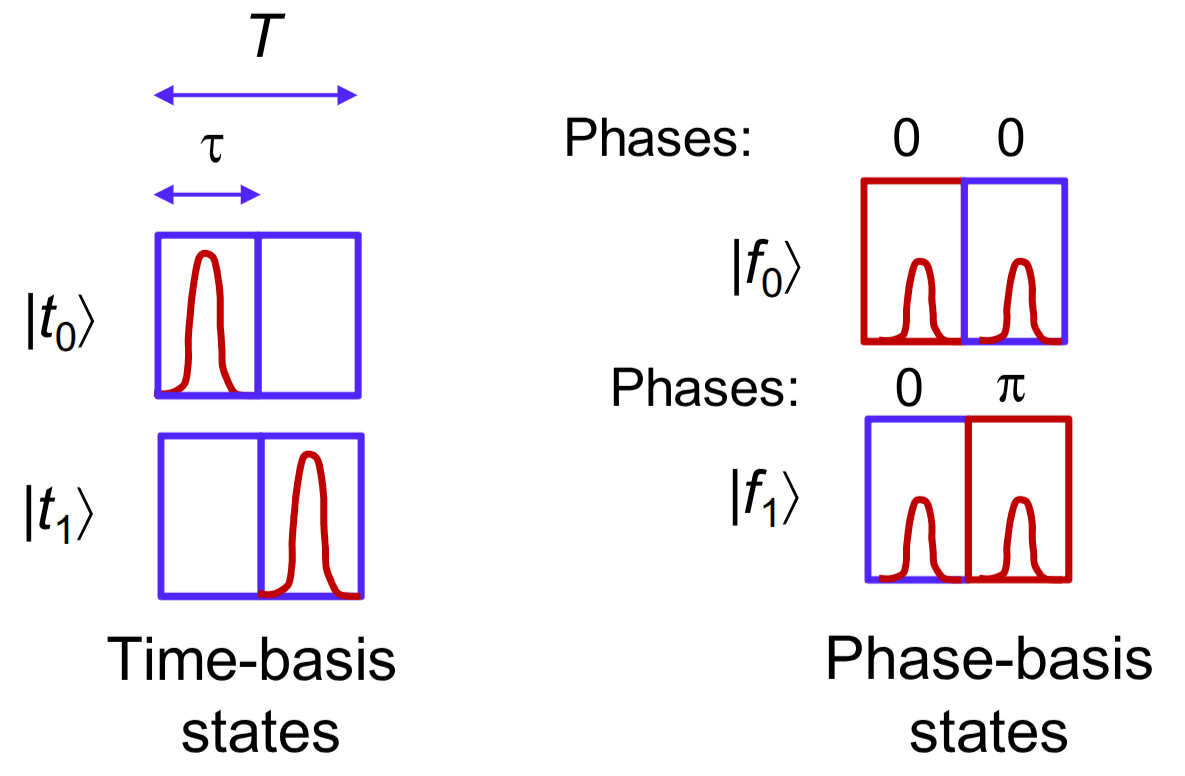
\includegraphics[width=0.8\textwidth]{chapters/figs/fig-6-7}
	\caption{حالت‌های کدگذاری فاز-زمان مورد استفاده در پروتکل \lr{BB84}.}
	\label{fig:6-7}
\end{figure}

\begin{figure}[ht]
	\centering
	 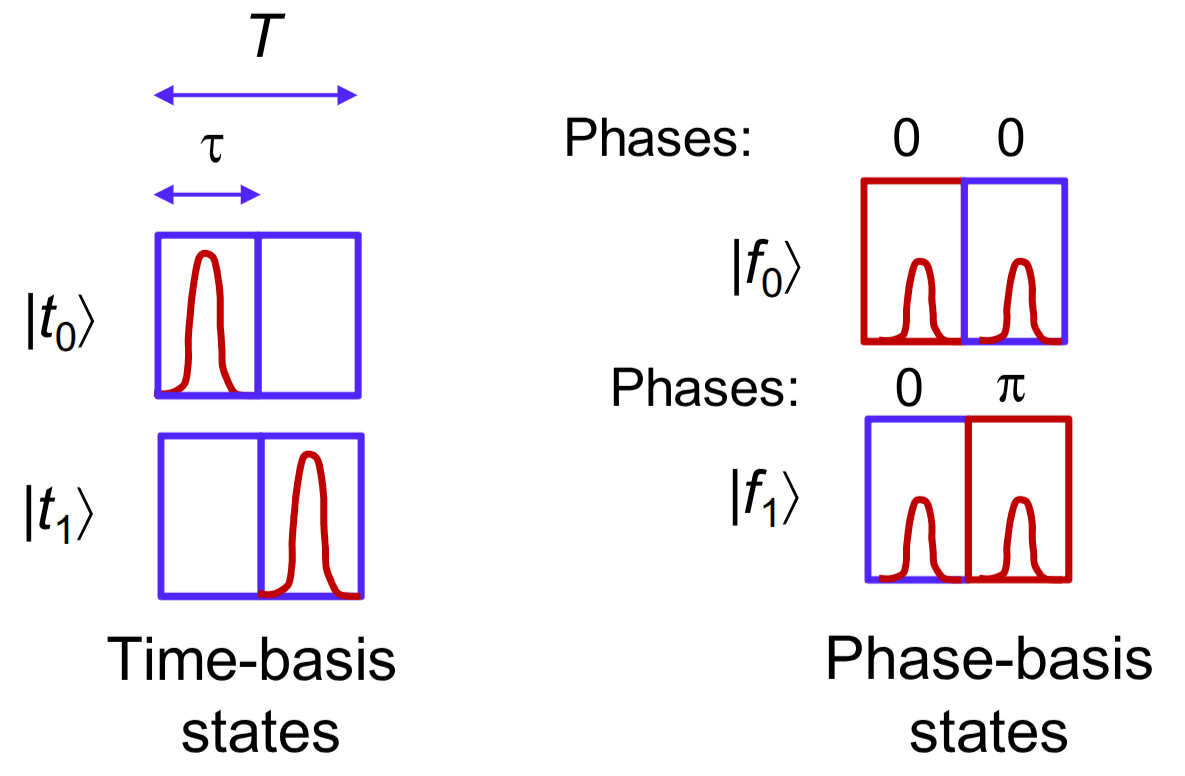
\includegraphics[width=0.8\textwidth]{chapters/figs/fig-6-8}
	\caption{رمزگذار فاز-زمان پروتکل توزیع کلید کوانتومی \lr{BB84}. \lr{AWG}: مولد شکل‌موج دلخواه؛ \lr{VOA}: تضعیف‌کننده نوری متغیر.}
	\label{fig:6-8}
\end{figure}

\begin{figure}[ht]
	\centering
	 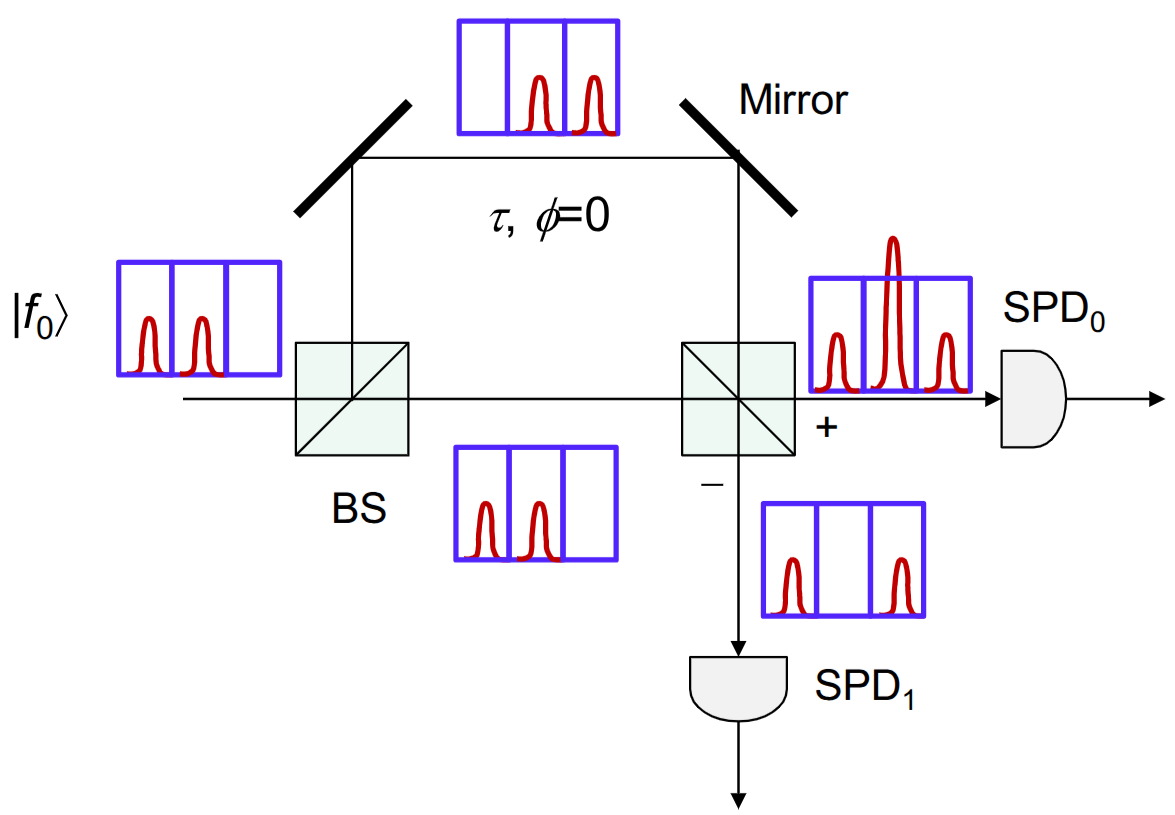
\includegraphics[width=0.8\textwidth]{chapters/figs/fig-6-9}
	\caption{رمزگشای فاز-زمان برای پروتکل توزیع کلید کوانتومی \lr{BB84}. \lr{BS}: تقسیم‌کننده پرتو $50:50$؛ \lr{SPD}: آشکارساز تک‌فوتون.}
	\label{fig:6-9}
\end{figure}

هنگامی که حالت فازی $|\phi_0\rangle$ به رمزگشای فاز-زمان وارد می‌شود، خروجی‌های دومین تقسیم‌کننده پرتو (\lr{BS}) ۵۰:۵۰ سه بازه زمانی را اشغال می‌کنند. خروجی $+$ موردی را نشان می‌دهد که در آن خروجی‌های تداخل‌سنج تداخل سازنده\LTRfootnote{Constructive interference} دارند، در حالی که خروجی $-$ نشان‌دهنده تداخل ویرانگر\LTRfootnote{Destructive interference} خروجی‌های متناظر تداخل‌سنج است. برای تداخل سازنده، پالس میانی دوبرابر می‌شود، در حالی که برای تداخل ویرانگر، پالس‌های میانی یکدیگر را خنثی می‌کنند. بنابراین، کلیک \lr{SPD} در بازه میانی در خروجی $+$، حالت $|\phi_0\rangle$ را شناسایی می‌کند و کلیک متناظر در خروجی $-$، حالت $|\phi_1\rangle$ را تشخیص می‌دهد.

\section{امنیت توزیع کلید کوانتومی}
\label{sec:6-5}
همان‌طور که در بخش مربوط به پروتکل \lr{BB84} بحث شد، آلیس و باب پس از اتمام مرحله ارسال کلید خام، فرآیند غربال‌گری و تخمین پارامتر\LTRfootnote{Parameter estimation} را انجام می‌دهند. از $N$ نماد ارسال شده، $n$ نماد باقی می‌ماند و کلید متناظر با آن‌ها، کلید غربال‌شده\LTRfootnote{Sifted key} نامیده می‌شود. پس از آن، آن‌ها پس‌پردازش کلاسیک مانند مصالحه اطلاعات و تقویت حریم خصوصی را انجام می‌دهند. در مرحله مصالحه اطلاعات، آن‌ها از تصحیح خطا برای اصلاح خطاهای ایجاد شده توسط کانال کوانتومی و ایو استفاده می‌کنند؛ کلید متناظر پس از اتمام این مرحله معمولاً کلید اصلاح‌شده\LTRfootnote{Corrected key} نامیده می‌شود. در طول تقویت حریم خصوصی، آن‌ها همبستگی باقی‌مانده با ایو را حذف می‌کنند و از $n$ نماد، $m$ نماد باقی می‌ماند که کلید متناظر، کلید امن\LTRfootnote{Secure key} است. به‌وضوح، نرخ کسر کلید مخفی $r$ را می‌توان به‌صورت $r = m/n$ (یا $m/N$) تعیین کرد که اغلب به آن کسر مخفی\LTRfootnote{Secret fraction} گفته می‌شود \cite{48}. نرخ کلید مخفی (\lr{SKR})\LTRfootnote{Secret-key rate (SKR)} سپس به‌صورت حاصل‌ضرب کسر مخفی $r$ و نرخ کلید خام $R_{\text{raw}}$ تعیین می‌شود و می‌توانیم بنویسیم \cite{48}:
\begin{equation}
	\text{SKR} = r \cdot R_{\text{raw}}
	\label{eq:6-22}
\end{equation}
جالب است که در بسیاری از مقالات، \lr{SKR} به همان کسر مخفی $r$ اشاره دارد. با توجه به اینکه نرخ کلید خام توسط دستگاه‌های مورد استفاده (به‌ویژه \lr{SPD}) و کانال کوانتومی که ارسال در آن صورت می‌گیرد تعیین می‌شود و نه توسط قوانین فیزیک کوانتوم، نرخ کسری را می‌توان نرخ \lr{SKR} نرمالیزه‌شده نیز نامید، به‌طوری که $r = \text{SKR}/R_{\text{raw}}$.

نرخ کلید خام را می‌توان به‌صورت حاصل‌ضرب نرخ سیگنال‌دهی $R_s$ و احتمال پذیرش نماد ارسالی توسط باب به‌طور میانگین، که با $\text{Pr}(\text{Bob accepting})$ نشان داده می‌شود، تعیین کرد؛ بنابراین می‌توانیم بنویسیم:
\begin{equation}
	R_{\text{raw}} = R_s \cdot \text{Pr}(\text{Bob accepting})
	\label{eq:6-23}
\end{equation}
از سوی دیگر، نرخ سیگنال‌دهی به‌صورت زیر تعیین می‌شود \cite{48}:
\begin{equation}
	R_s = \min \left\{ R_{s,\text{max}}, \frac{1}{T_{dc}}, \frac{1}{\mu T T_B \eta \tau_{\text{dead}}} \right\}
	\label{eq:6-24}
\end{equation}
که در آن $R_{s,\text{max}}$ حداکثر نرخ سیگنال‌دهی مجاز توسط منبع، $T_{dc}$ چرخه کاری\LTRfootnote{Duty cycle} و $\tau_{\text{dead}}$ زمان مرده\LTRfootnote{Dead time} مربوط به \lr{SPD} (زمان مورد نیاز برای بازنشانی \lr{SPD} پس از آشکارسازی یک فوتون) است. عبارت $\mu T T_B \eta$ متناظر با احتمال آشکارسازی باب است؛ $\mu$ میانگین تعداد فوتون‌های تولید شده توسط منبع، $\eta$ بازدهی \lr{SPD}، $T$ گذردهی\LTRfootnote{Transmissivity} کانال کوانتومی و $T_B$ نشان‌دهنده تلفات در گیرنده باب است. کانال کوانتومی معمولاً یک فیبر نوری یا یک کانال نوری فضای آزاد است. تضعیف در کانال فیبر نوری با $T = 10^{-\alpha L/10}$ تعیین می‌شود که در آن $\alpha$ ضریب تضعیف برحسب \lr{dB/km} و $L$ مسافت ارسال برحسب \lr{km} است. ضریب تضعیف معمول در فیبر تک‌مد استاندارد (\lr{SSMF})\LTRfootnote{Standard single-mode fiber (SSMF)} در طول موج ۱۵۵۰ نانومتر، $0.2$ \lr{dB/km} است. در مورد پیوند \lr{FSO}، اگر از اثرات تلاطم اتمسفری صرف‌نظر کنیم، برای یک پیوند خط دید\LTRfootnote{Line-of-sight} با مسافت ارسال $L$، می‌توانیم تلفات پیوند \lr{FSO} را طبق مرجع \cite{49} به‌صورت زیر تخمین بزنیم:
\begin{equation*}
	T = \left[ \frac{d_{Rx}}{d_{Tx} + DL} \right]^2 \cdot 10^{-\alpha L/10}
\end{equation*}
که در آن $d_{Tx}$ و $d_{Rx}$ قطر دهانه تلسکوپ‌های فرستنده و گیرنده و $D$ واگرایی\LTRfootnote{Divergence} است. بنابراین، جمله اول نشان‌دهنده تلفات هندسی و جمله دوم تضعیف میانگین ناشی از پراکندگی\LTRfootnote{Scattering} است، که ضریب تضعیف پراکندگی در شرایط آسمان صاف در محدوده ۱۵۲۰ تا ۱۶۰۰ نانومتر کمتر از $0.1$ \lr{dB/km} است.

در پروتکل \lr{BB84}، احتمالی که باب نماد ارسالی را می‌پذیرد به احتمال استفاده او از پایه یکسان مربوط است که با $p_{\text{sift}}$ نشان داده می‌شود، به‌طوری که نرخ سیگنال‌دهی به‌صورت $R_s p_{\text{sift}}$ در می‌آید و نرخ کلید خام زمانی که آلیس $n$ فوتون برای باب ارسال می‌کند، برابر خواهد بود با \cite{48}:


\begin{equation}
	R_{\text{raw},n} = R_s p_{\text{sift}} p_{A,n} p_n
	\label{eq:6-25}
\end{equation}
که در آن $p_{A,n}$ احتمال این است که پالس ارسال شده توسط آلیس شامل $n$ فوتون باشد (بخش زیر را ببینید) و $p_n$ احتمال این است که ایو پالسی با $n$ فوتون برای باب ارسال کند. نرخ کلید خام کل برابر با $R_{\text{raw}} = \sum_n R_{\text{raw},n}$ خواهد بود.

آنچه باقی مانده، تعیین نرخ کسر (تفاضلی) است. \lr{QKD} می‌تواند به امنیت غیرمشروط\LTRfootnote{Unconditional security} دست یابد، به این معنی که امنیت آن بدون اعمال هیچ‌گونه محدودیتی بر توان محاسباتی یا استراتژی شنود ایو، قابل تأیید است. کران‌های نرخ کسر به مراحل پس‌پردازش کلاسیک بستگی دارد. رایج‌ترین روش، پس‌پردازش یک‌طرفه\LTRfootnote{One-way postprocessing} است که در آن آلیس یا باب کلید مرجع را نگه داشته و اطلاعات کلاسیک را از طریق کانال عمومی برای طرف دیگر ارسال می‌کند، در حالی که طرف مقابل بدون ارائه بازخورد، فرآیند خاصی را روی داده‌ها انجام می‌دهد. معمول‌ترین پردازش یک‌طرفه شامل دو مرحله مصالحه اطلاعات و تقویت حریم خصوصی است. رابطه کسر مخفی به‌دست‌آمده از پس‌پردازش یک‌طرفه در مرجع \cite{48} به‌صورت زیر داده شده است:
\begin{equation}
	r = I(\bm{A}; \bm{B}) - \min_{\text{Eve's strategies}} (I_{EA}, I_{EB})
	\label{eq:6-26}
\end{equation}
که در آن $I(\bm{A}; \bm{B})$ اطلاعات متقابل بین آلیس و باب است، در حالی که جمله دوم متناظر با اطلاعات ایو $I_E$ درباره کلید خام آلیس یا باب است و کمینه‌سازی روی تمام استراتژی‌های شنود ممکن انجام می‌شود. آلیس و باب تصمیم می‌گیرند که از مصالحه مستقیم یا معکوس استفاده کنند تا بتوانند اطلاعات ایو را کمینه کنند.

اکنون استراتژی‌های مختلف شنود را که ایو ممکن است به کار گیرد و اطلاعات ایو $I_E$ را تعیین می‌کنند، شرح می‌دهیم.

\subsubsection{حملات مستقل (انفرادی) یا غیرهمدوس}
\label{subsec:6-5-1}
این محدودترین خانواده از حملات است که در آن ایو به هر کیوبیت به‌طور مستقل حمله کرده و با اعمال استراتژی یکسان با هر کیوبیت تعامل می‌کند. علاوه بر این، او حالت‌های کوانتومی را پیش از انجام پس‌پردازش کلاسیک اندازه‌گیری می‌کند. کران امنیت برای حملات غیرهمدوس\LTRfootnote{Incoherent attacks} مشابه امنیت لایه فیزیکی (\lr{PLS}) کلاسیک \cite{2} است و توسط حد سیزار-کورنر\LTRfootnote{Csiszár-Körner bound} \cite{50} تعیین می‌شود که در رابطه \eqref{eq:6-26} داده شده است و در آن اطلاعات متقابل بین آلیس و ایو به‌صورت زیر است:
\begin{equation}
	I_{EA} = \max_{\text{Eve's strategies}} I(\bm{A}; \bm{E})
	\label{eq:6-27}
\end{equation}
که در آن بیشینه‌سازی روی تمام استراتژی‌های شنود غیرهمدوس ممکن انجام می‌شود. تعریف مشابهی برای $I_{BE}$ نیز برقرار است.

خانواده مهمی از حملات غیرهمدوس، حملات سد کردن-بازارسال\LTRfootnote{Intercept-resend (IR) attacks} (\lr{IR}) هستند؛ که در آن ایو سیگنال کوانتومی ارسال شده توسط آلیس را سد کرده، اندازه‌گیری را روی آن انجام می‌دهد و بر اساس نتیجه اندازه‌گیری، سیگنال کوانتومی جدیدی را (در همان \lr{MUB} حالت کوانتومی اندازه‌گیری شده) آماده کرده و آن را برای باب ارسال می‌کند. در پروتکل \lr{BB84}، انتخاب پایه توسط ایو در ۵۰٪ مواقع با پایه آلیس مطابقت دارد. زمانی که او از پایه اشتباه استفاده می‌کند، باز هم ۵۰٪ شانس برای حدس زدن بیت صحیح دارد. وقتی باب اندازه‌گیری را انجام می‌دهد، ۵۰٪ احتمال دارد که باب از همان پایه ایو استفاده کند. با این حال، این بیت‌ها با دنباله ایو همبستگی خواهند داشت و نه با آلیس، و احتمال کلی خطا ۱/۴ خواهد بود، در حالی که اطلاعات متقابل بین آلیس و ایو $I(\bm{A}; \bm{E}) = 1/2$ است. با توجه به احتمال خطای بالای ایجاد شده توسط حمله \lr{IR}، آلیس و باب می‌توانند به راحتی فعالیت ایو را شناسایی کنند. با این حال، ایو ممکن است تصمیم بگیرد حمله \lr{IR} را با احتمال $p_{IR}$ اعمال کند. در آن صورت احتمال خطا $q = p_{IR}/4$ خواهد بود. اطلاعات متقابل بین آلیس و ایو در این صورت $I(\bm{A}; \bm{E}) = h(p_{IR}/4)$ خواهد بود، که در آن $h(\cdot)$ تابع آنتروپی باینری\LTRfootnote{Binary entropy function} $h(q) = -q \log_2 q - (1-q) \log_2 (1-q)$ است. اگر تمام خطاها به ایو نسبت داده شود، کسر مخفی را می‌توان به‌صورت زیر تخمین زد:
\begin{equation}
	r = \underbrace{1 - h(q)}_{I(\bm{A}; \bm{B})} - h(q) = 1 - 2h(q)
	\label{eq:6-28}
\end{equation}

خانواده مهم دیگری از حملات غیرهمدوس، حملات \lr{PNS} هستند \cite{51} که در آن ایو روی حالت‌های کوانتومی چندفوتونی عمل می‌کند. در یک سیستم \lr{QKD} مبتنی بر \lr{WCS}، حالت‌های کوانتومی با مدوله کردن باریکه از منبع نور همدوس تولید می‌شوند که سپس تضعیف می‌گردد تا به‌طور میانگین یک فوتون در هر پالس توسط آلیس ارسال شود. با این حال، همان‌طور که پیش‌تر بحث شد، منبع همدوس فوتون‌ها را بر اساس توزیع پواسون گسیل می‌کند، به‌طوری که احتمال گسیل $n$ فوتون در حالتی با میانگین تعداد فوتون تولید شده $\mu$ توسط معادله زیر تعیین می‌شود:
\begin{equation}
	p_{A,n} = p(n|\mu) = \frac{e^{-\mu} \mu^n}{n!}
	\label{eq:6-29}
\end{equation}
با افزایش پارامتر $\mu$، احتمال دریافت بیش از یک فوتون نیز افزایش می‌یابد. برای انجام حمله \lr{PNS}، ایو می‌تواند از تقسیم‌کننده پرتو برای برداشتن یکی از فوتون‌ها از حالت چندفوتونی استفاده کند و بقیه را به باب انتقال دهد، همان‌طور که در شکل \ref{fig:6-10} تصویر شده است. او می‌تواند فوتون را با انتخاب تصادفی پایه اندازه‌گیری کند. ایو حتی می‌تواند پیوند کوانتومی را با فیبر با تلفات بسیار کم جایگزین کند تا آلیس و باب نتوانند تشخیص دهند که سیگنال ارسالی تضعیف شده است. برای حل مشکل حمله \lr{PNS}، آلیس و باب می‌توانند از پروتکل مبتنی بر حالت فریب \cite{37} استفاده کنند که در آن آلیس حالت‌های کوانتومی را با میانگین تعداد فوتون‌های متفاوت (نشان‌دهنده حالت‌های سیگنال و فریب) ارسال می‌کند. ایو نمی‌تواند بین حالت‌های فریب و سیگنال تمایز قائل شود و با توجه به اینکه آلیس و باب سطح سیگنال فریب را می‌دانند، می‌توانند حمله \lr{PNS} را شناسایی کنند.

\subsubsection{حملات دسته‌جمعی}
\label{subsec:6-5-2}
حملات دسته‌جمعی\LTRfootnote{Collective attacks} نشان‌دهنده تعمیمی از حملات غیرهمدوس هستند، با این فرض که تعامل ایو با هر کیوبیت نیز به‌صورت مستقل و با توزیع یکسان (\lr{i.i.d.})\LTRfootnote{Independent and identically distributed (i.i.d.)} است. با این حال، در این حملات، ایو می‌تواند کیوبیت‌های کمکی\LTRfootnote{Ancilla qubits} خود را تا پایان مراحل پس‌پردازش کلاسیک در یک حافظه کوانتومی ذخیره کند. برای مثال، با توجه به اینکه مصالحه اطلاعات مستلزم تبادل بیت‌های توازن\LTRfootnote{Parity bits} روی یک کانال کلاسیک احرازهویت‌شده است، ایو می‌تواند بهترین حملات کلاسیک شناخته‌شده را برای یادگیری محتوای بیت‌های توازن به کار گیرد. بر اساس تمام اطلاعات در دسترس، ایو می‌تواند بهترین استراتژی اندازه‌گیری را روی کیوبیت‌های کمکی خود (ذخیره شده در حافظه کوانتومی) انجام دهد.

حمله \lr{PNS} زمانی که ایو از حافظه کوانتومی استفاده می‌کند قوی‌تر است. به‌ویژه، ایو می‌تواند از طریق فرآیند غربال‌گری متوجه شود که کدام پایه توسط آلیس استفاده شده است و می‌تواند پایه صحیح را روی فوتون ذخیره شده در حافظه کوانتومی خود اعمال کند و در نتیجه تعداد بیت‌های شناسایی شده را در مقایسه با حالتی که از حافظه کوانتومی استفاده نمی‌شود، دوبرابر کند.

کران امنیت برای حملات دسته‌جمعی، با فرض پس‌پردازش یک‌طرفه، توسط رابطه \eqref{eq:6-26} داده می‌شود که در آن اطلاعات ایو درباره دنباله آلیس از طریق اطلاعات هولِوو\LTRfootnote{Holevo information} به‌صورت زیر تعیین می‌شود \cite{52}:

\begin{figure}[ht]
	\centering
	 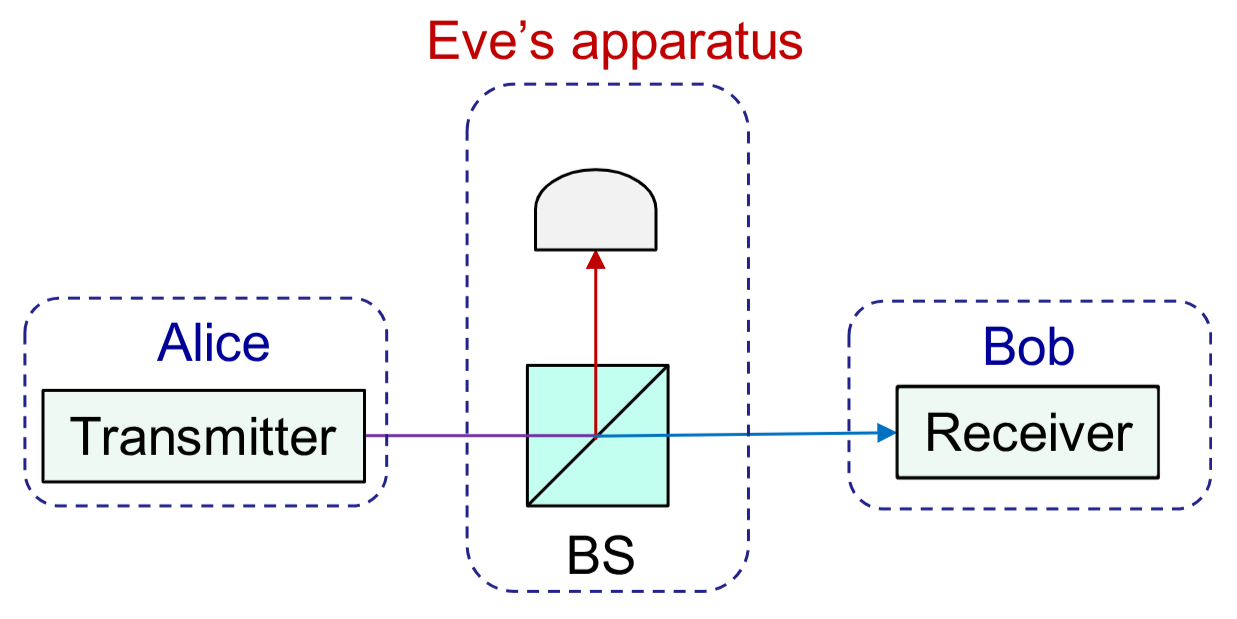
\includegraphics[width=0.7\textwidth]{chapters/figs/fig-6-10}
	\caption{تصویرسازی اجرای حمله تقسیم تعداد فوتون توسط ایو. \lr{BS}: تقسیم‌کننده پرتو.}
	\label{fig:6-10}
\end{figure}



\begin{equation}
	I_{EA} = \max_{\text{Eve's strategies}} \chi(\bm{A}; \bm{E})
	\label{eq:6-30}
\end{equation}
که در آن بیشینه‌سازی روی تمام استراتژی‌های شنود دسته‌جمعی ممکن انجام می‌شود. این کران با نام کران دوتک-وینتر\LTRfootnote{Devetak-Winter bound} نیز شناخته می‌شود. اطلاعات هولِوو که در مرجع \cite{53} معرفی شده است، در اینجا به‌صورت زیر تعریف می‌شود:
\begin{equation}
	\chi(\bm{A}; \bm{E}) = S(\rho_E) - \sum_a p(a) S(\rho_{E|a})
	\label{eq:6-31}
\end{equation}
که در آن $S(\rho)$ آنتروپی فون نویمان\LTRfootnote{von Neumann entropy} است که به‌صورت $S(\rho) = -\text{Tr}(\rho \log \rho) = -\sum_i \lambda_i \log \lambda_i$ تعریف می‌شود و در آن $\lambda_i$ مقادیر ویژه عملگر (حالت) چگالی $\rho$ هستند. در رابطه \eqref{eq:6-31}، $p(a)$ نشان‌دهنده احتمال وقوع نماد $a$ از الفبای کلاسیک آلیس است، در حالی که $\rho_{E|a}$ عملگر چگالی متناظر با سیستم کمکی\LTRfootnote{Ancilla} ایو است. در نهایت، $\rho_E$ حالت چگالی جزئی ایو است که به‌صورت $\rho_E = \sum_a p(a) \rho_{E|a}$ تعریف می‌شود. به عبارت دیگر، اطلاعات هولِوو متناظر با میانگین کاهش در آنتروپی فون نویمان است، با این فرض که می‌دانیم $\rho_E$ چگونه آماده‌سازی شده است.



\subsubsection{حملات هک کوانتومی و حملات کانال جانبی}
\label{subsec:6-5-3}
حملات هک کوانتومی\LTRfootnote{Quantum hacking attacks} از نقاط ضعف پیاده‌سازی‌های خاص سیستم‌های \lr{QKD} بهره‌برداری می‌کنند. بسیاری از این حملات هک با فناوری کنونی امکان‌پذیر هستند. در یک حمله اسب تروا\LTRfootnote{Trojan horse attack} \cite{54}، ایو یک باریکه لیزری درخشان را به سمت رمزگذار آلیس می‌فرستد و فوتون‌های بازتابیده را برای کسب اطلاعات درباره کلید مخفی اندازه‌گیری می‌کند. با استفاده از یک ایزولاتور نوری\LTRfootnote{Optical isolator} می‌توان از این حمله جلوگیری کرد. همچنین مشاهده شده است که شمارنده‌های فوتون مبتنی بر سیلیسیم که از فوتودیودهای بهمنی\LTRfootnote{Avalanche photodiodes (APDs)} (\lr{APD}) استفاده می‌کنند، هنگام آشکارسازی یک تک‌فوتون، مقداری نور در طول‌موج‌های مختلف ساطع می‌کنند که می‌تواند توسط ایو مورد بهره‌برداری قرار گیرد \cite{55}. در حمله جابه‌جایی زمانی\LTRfootnote{Time-shifting attack} \cite{56}، ایو از عدم تطابق بازدهی \lr{SPD}های باب برای تخمین انتخاب پایه توسط او استفاده می‌کند. در یک حمله کورسازی\LTRfootnote{Blinding attack} \cite{57}، ایو از ویژگی‌های شمارنده تک‌فوتون مبتنی بر \lr{APD} بهره می‌گیرد تا باب را مجبور کند همان پایه‌ای را انتخاب کند که ایو انتخاب کرده است. \lr{APD}ها برای شمارش فوتون اغلب در مد گیت‌شده\LTRfootnote{Gated mode} عمل می‌کنند، به این معنی که \lr{APD} تنها زمانی فعال است که انتظار ورود فوتون می‌رود. وقتی \lr{APD} در وضعیت غیرفعال (خاموش) است، در یک رژیم خطی\LTRfootnote{Linear regime} عمل می‌کند، به این معنی که جریان نوری با توان نوری دریافتی متناسب است و بنابراین مانند یک فتودتکتور کلاسیک رفتار می‌کند. برای بهره‌برداری از این موضوع، ایو می‌تواند یک باریکه نور کلاسیک ضعیف ارسال کند که به اندازه کافی قوی باشد تا زمانی که باب از همان پایه ایو استفاده می‌کند «کلیک» ایجاد کند، و در غیر این صورت کلیکی ثبت نشود. در چنین سناریویی، ۵۰٪ از رویدادها به عنوان بی‌نتیجه ثبت می‌شوند. خوشبختانه، ویژگی مشترک حملات هک کوانتومی این است که به محض شناخته شدن حمله، قابل پیشگیری هستند. با این حال، تهدید ناشی از حملات هک کوانتومی ناشناخته همچنان پابرجاست.

بسیاری از حملات کانال جانبی\LTRfootnote{Side-channel attacks} به‌طور هم‌زمان حملات زمان خطای صفر\LTRfootnote{Time zero-error attacks} هستند \cite{48}. به بیان دیگر، ایو می‌تواند از تلفات کانال کوانتومی برای پنهان کردن حمله کانال جانبی خود استفاده کند. حمله تقسیم پرتو\LTRfootnote{Beam-splitting attack} از تلفات کانال کوانتومی بهره‌برداری می‌کند؛ ایو می‌تواند یک تقسیم‌کننده پرتو را دقیقاً بعد از فرستنده آلیس قرار دهد، بخشی از باریکه را برداشته و بقیه را به باب انتقال دهد. از آنجا که آلیس مد نوری را تغییر نمی‌دهد، این حمله توسط باب شناسایی نخواهد شد. جالب اینجاست که توزیع پواسون در طول حمله \lr{PNS} حفظ می‌شود \cite{58}. در پیاده‌سازی‌های واقع‌گرایانه، زمانی که آلیس از حالت‌های سیگنال مستقل خطی استفاده می‌کند، ایو می‌تواند تمایز ابهام‌ناپذیر حالت\LTRfootnote{Unambiguous state discrimination} را انجام داده و متعاقب آن سیگنال را مجدداً ارسال کند و به بازدهی بهتری نسبت به تقسیم پرتو دست یابد، همان‌طور که در مرجع \cite{59} نشان داده شده است. خوشبختانه، وجود حملات کانال جانبی تا زمانی که حملات مربوطه در مرحله تقویت حریم خصوصی در نظر گرفته شوند، امنیت را به خطر نمی‌اندازد \cite{48}.

\subsubsection{امنیت پروتکل BB84}
\label{subsec:6-5-4}
کران پایین کسر مخفی که با پروتکل \lr{BB84} قابل دستیابی است، توسط رابطه زیر داده می‌شود:
\begin{equation}
	r = q(Z)_1 [1 - h_2(e(X)_1)] - f_e q(Z) h_2(e(Z))
	\label{eq:6-32}
\end{equation}
که در آن $q(Z)_1$ نشان‌دهنده احتمال اعلام یک نتیجه موفقیت‌آمیز («بهره»\LTRfootnote{Gain}) در زمانی است که آلیس یک تک‌فوتون ارسال کرده و باب آن را در پایه $Z$ آشکار کرده است؛ $f_e$ نشان‌دهنده ناکارآمدی تصحیح خطا ($f_e \geq 1$) است؛ $e(X)$ [$e(Z)$] نشان‌دهنده نرخ خطای بیت کوانتومی\LTRfootnote{Quantum bit error rate (QBER)} (\lr{QBER}) در پایه $X$ (پایه $Z$) است؛ و $h_2(x)$ تابع آنتروپی باینری است که به‌صورت زیر تعریف می‌شود:
\begin{equation}
	h_2(x) = -x \log_2(x) - (1-x) \log_2(1-x)
	\label{eq:6-33}
\end{equation}
جمله دوم یعنی $q(Z)_1 h_2[e(X)_1]$ نشان‌دهنده مقدار اطلاعاتی است که ایو توانسته در طول ارسال کلید خام به‌دست آورد و این اطلاعات معمولاً در مرحله تقویت حریم خصوصی از کلید نهایی حذف می‌شود. جمله آخر یعنی $f_e q(Z) h_2[e(Z)]$ نشان‌دهنده مقدار اطلاعات فاش شده در مرحله مصالحه اطلاعات (تصحیح خطا) است که معمولاً به بیت‌های توازن تبادل شده در یک کانال عمومی بدون نویز مربوط می‌شود (زمانی که از تصحیح خطای سیستماتیک استفاده می‌شود).

\section{پروتکل‌های حالت فریب}
\label{sec:6-6}
هنگامی که به جای یک منبع تک‌فوتون از یک منبع حالت همدوس ضعیف (\lr{WCS}) استفاده می‌شود، این طرح نسبت به حمله \lr{PNS} حساس خواهد بود. با توجه به اینکه احتمال ارسال چندین فوتون از \lr{WCS} اکنون غیرصفر است، ایو می‌تواند از این واقعیت برای کسب اطلاعات از کانال بهره‌برداری کند. برای غلبه بر حمله \lr{PNS}، استفاده از سیستم‌های توزیع کلید کوانتومی مبتنی بر حالت فریب\LTRfootnote{Decoy-state} در مراجع \cite{37, 61, 62, 63, 64, 65, 66, 67, 68, 69, 70} پیشنهاد شده است. در \lr{QKD} حالت فریب، میانگین تعداد فوتون‌های ارسالی در بازه‌های زمانی تصادفی افزایش می‌یابد که به آلیس و باب اجازه می‌دهد تشخیص دهند که آیا در زمان ارسال چندین فوتون، ایو در حال سرقت فوتون‌ها است یا خیر. نسخه‌های مختلفی از پروتکل‌های مبتنی بر حالت فریب وجود دارد. در پروتکل مبتنی بر یک-حالت-فریب، علاوه بر حالت سیگنال با میانگین تعداد فوتون $\mu$، حالت فریب با میانگین تعداد فوتون $\nu < \mu$ نیز به کار گرفته می‌شود. آلیس ابتدا درباره سطوح میانگین تعداد فوتون سیگنال و فریب تصمیم‌گیری کرده و سپس بر اساس رابطه \lr{SKR} متناظر، احتمالات بهینه برای استفاده از این دو سطح را تعیین می‌کند. در پروتکل مبتنی بر «حالت فریب ضعیف به‌علاوه خلاء»، علاوه بر سطوح $\mu$ و $\nu$، از حالت خلاء\LTRfootnote{Vacuum state} نیز به عنوان حالت فریب استفاده می‌شود. هر دو پروتکل در مرجع \cite{67} به‌صورت تئوری و تجربی ارزیابی شده‌اند. نتیجه‌گیری شد که استفاده از یک حالت سیگنال و دو حالت فریب کافی است، که این موضوع با یافته‌های مراجع \cite{68, 69} مطابقت دارد.

احتمالی که آلیس بتواند فوتون را با موفقیت آشکارسازی کند، زمانی که از \lr{WCS} با میانگین تعداد فوتون $\mu$ استفاده می‌کند، با $q_\mu$ نشان داده می‌شود و به عنوان بهره\LTRfootnote{Gain} شناخته می‌شود که می‌تواند توسط رابطه زیر تعیین گردد:
\begin{equation}
	q_\mu = \sum_{n=0}^{\infty} y_n \frac{e^{-\mu} \mu^n}{n!}
	\label{eq:6-34}
\end{equation}
که در آن $y_n$، که به عنوان بازده\LTRfootnote{Yield} نیز شناخته می‌شود، احتمال آشکارسازی موفقیت‌آمیز باب در زمانی است که آلیس $n$ فوتون ارسال کرده است. رابطه مشابهی برای حالت‌های فریب با میانگین تعداد فوتون $\nu_i$ برقرار است، یعنی:
\begin{equation}
	q_{\nu_i} = \sum_{n=0}^{\infty} y_n \frac{e^{-\nu_i} \nu_i^n}{n!}
	\label{eq:6-35}
\end{equation}

اگر $e_n$ نشان‌دهنده \lr{QBER} متناظر با حالتی باشد که آلیس $n$ فوتون ارسال کرده است، میانگین \lr{QBER} برای حالت همدوس $|\sqrt{\mu} \exp(j\phi)\rangle$ (که در آن $\phi$ فاز دلخواه است) را می‌توان به‌صورت زیر تخمین زد:
\begin{equation}
	e_\mu = \frac{1}{q_\mu} \sum_{n=0}^{\infty} y_n e_n \frac{e^{-\mu} \mu^n}{n!}
	\label{eq:6-36}
\end{equation}

اگر $\eta_{\text{all}}$ بازدهی کل ارسال، متشکل از گذردهی کانال $T_{ch}$، بازدهی فتودتکتور $\eta$ و گذردهی بخش نوری باب $T_{\text{Bob}}$ باشد، بازدهی ارسال پالس $n$-فوتونی به‌صورت زیر خواهد بود:
\begin{equation}
	T_n = 1 - (1 - \eta_{\text{all}})^n
	\label{eq:6-37}
\end{equation}

در غیاب ایو، برای $n=0$، بازده $y_0$ تحت تأثیر نرخ آشکارسازی پس‌زمینه که با $p_d$ نشان داده می‌شود، قرار دارد؛ بنابراین می‌توانیم بنویسیم $y_0 = p_d$. از سوی دیگر، بازده برای $n \geq 1$ توسط هر دو عامل فوتون‌های سیگنال و نرخ پس‌زمینه به صورت زیر تعیین می‌شود:
\begin{equation}
	y_n = T_n + y_0 - T_n y_0 = T_n + y_0(1 - T_n) = 1 - (1 - y_0)(1 - \eta_{\text{all}})^n
	\label{eq:6-38}
\end{equation}

نرخ خطای حالت‌های $n$-فوتونی $e_n$ را می‌توان طبق مراجع \cite{37, 70} به‌صورت زیر تخمین زد:
\begin{equation}
	e_n = \frac{1}{y_n} \left[ e_0 y_0 + e_d T_n \right] \approx e_d + \frac{y_0}{y_n} (e_0 - e_d)
	\label{eq:6-39}
\end{equation}
که در آن $e_d$ احتمال برخورد یک فوتون به یک آشکارساز اشتباه است. برای کدگذاری فاز-زمان، این مقدار نشان‌دهنده نرخ خطای عدم انطباق ذاتی\LTRfootnote{Intrinsic misalignment error rate} است. در غیاب فوتون‌های سیگنال، با فرض اینکه دو آشکارساز دارای نرخ‌های پس‌زمینه یکسانی هستند، می‌توانیم بنویسیم $e_0 = 1/2$. به‌طور مشابه، میانگین \lr{QBER} را می‌توان به‌صورت زیر تخمین زد:
\begin{equation}
	e_\mu = e_d + \frac{y_0}{q_\mu} (e_0 - e_d)
	\label{eq:6-40}
\end{equation}

اکنون می‌توان کران پایین کسر امنیت را با اصلاح رابطه مربوط به پروتکل‌های \lr{BB84} به‌صورت زیر تعیین کرد:
\begin{equation}
	r = q(Z)_1 [1 - h_2(e(X)_1)] - q(Z)_\mu f_e h_2(e(Z)_\mu)
	\label{eq:6-41}
\end{equation}
که در آن زیرنویس $1$ نشان‌دهنده پالس‌های تک‌فوتونی و زیرنویس $\mu$ نشان‌دهنده پالسی با میانگین تعداد فوتون $\mu$ است.

به‌عنوان یک نمونه، شکل \ref{fig:6-11} نتایج کسر امنیت را برای پروتکل حالت فریب و پروتکل آماده‌سازی-و-اندازه‌گیری \lr{BB84} مبتنی بر \lr{WCS}، با فرض استفاده از فیبر تک‌مد استاندارد (\lr{SMF}) با ضریب تضعیف $0.21$ \lr{dB/km} ارائه می‌دهد.

سایر پارامترهای استفاده شده در شبیه‌سازی‌ها به‌صورت زیر تنظیم شده‌اند \cite{37, 71, 72, 73}: بازدهی آشکارساز $\eta = 0.045$، نرخ شمارش تاریک $p_d = 1.7 \times 10^{-6}$، احتمال برخورد فوتون به آشکارساز اشتباه $e_d = 0.033$ و ناکارآمدی مصالحه $f_e = 1.22$. برای پروتکل \lr{BB84} مبتنی بر حالت فریب، جهت محاسبه کسر امنیت، از رابطه \eqref{eq:6-41} برای مقدار بهینه میانگین تعداد فوتون در هر پالس $\mu$ استفاده می‌کنیم که در آن $q_\mu$ توسط $q_\mu = 1 - (1 - y_0)\exp(-\mu \eta_{\text{all}})$ تعیین می‌شود، $e_\mu$ توسط رابطه \eqref{eq:6-40}، $e_1$ توسط رابطه \eqref{eq:6-39} و $q_1$ به عنوان آرگومان \eqref{eq:6-34} برای $n=1$ یعنی توسط $q_1 = y_1 \mu \exp(-\mu)$ تعیین می‌گردد. برای پروتکل \lr{BB84} مبتنی بر \lr{WCS} بدون حالت فریب، از رابطه \eqref{eq:6-41} با این فرض استفاده می‌کنیم که ایو کانال را کنترل می‌کند، حملات سد کردن-بازارسال را انجام می‌دهد و نسبت به حالت‌های چندفوتونی شفاف است. در این سناریوی کران پایین، خطای ناشی از رویدادهای تک‌فوتونی غالب است. اکنون با محاسبه $q(Z)$ توسط $q_\mu = 1 - (1 - y_0)\exp(-\mu \eta_{\text{all}})$ و $e(Z)$ توسط $E_\mu = e_d + (e_0 - e_d)y_0/q_\mu$ و با فرض $\mu$ غیربهینه متناسب با $\eta_{\text{all}}$، منحنی زرد رنگ در شکل \ref{fig:6-11} به‌دست آمد که با مرجع \cite{37} مطابقت دارد. هنگامی که به جای آن از $\mu$ بهینه (که کسر امنیت را بیشینه می‌کند) استفاده می‌کنیم، منحنی بنفش به‌دست می‌آید که با مرجع \cite{71} مطابقت دارد. برای این دو منحنی، مقدار $q(Z)_1$ را از \eqref{eq:6-34} با قرار دادن $y_n = 1$ برای $n \geq 2$ (ببینید مرجع \cite{70}) به‌صورت زیر تخمین می‌زنیم:
\begin{equation}
	q(X)_1 \approx q_\mu - \sum_{n=2}^{\infty} \frac{e^{-\mu} \mu^n}{n!}
	\label{eq:6-42}
\end{equation}
با توجه به اینکه حالت‌های چندفوتونی خطایی ایجاد نمی‌کنند (یعنی $e_n = 0$ برای $n \geq 2$)، می‌توانیم $e_1$ را به‌صورت زیر محدود کنیم:
\begin{equation}
	e(X)_1 \approx q_\mu E_\mu / q(X)_1
	\label{eq:6-43}
\end{equation}
رابطه دقیق‌تر برای $q_\mu$ در پروتکل \lr{BB84} مبتنی بر \lr{WCS} به‌صورت زیر خواهد بود:
\begin{equation}
	q_\mu = y_0 e^{-\mu} + y_1 e^{-\mu} \mu + \sum_{n=2}^{\infty} \frac{e^{-\mu} \mu^n}{n!}
	\label{eq:6-44}
\end{equation}
که از رابطه \eqref{eq:6-34} با قرار دادن $y_n = 1$ برای $n \geq 2$ به‌دست می‌آید. منحنی متناظر با رنگ صورتی نشان داده شده است که نشان می‌دهد با استفاده از پروتکل \lr{BB84} مبتنی بر \lr{WCS}، مسافت $L = 48.62$ کیلومتر قابل دستیابی است. در مقابل، برای پروتکل \lr{BB84} مبتنی بر حالت فریب و $\mu$ بهینه، دستیابی به مسافت نزدیک به $141.8$ کیلومتر امکان‌پذیر است (منحنی آبی را ببینید) که با مرجع \cite{71} مطابقت دارد.

\begin{figure}[ht]
	\centering
	 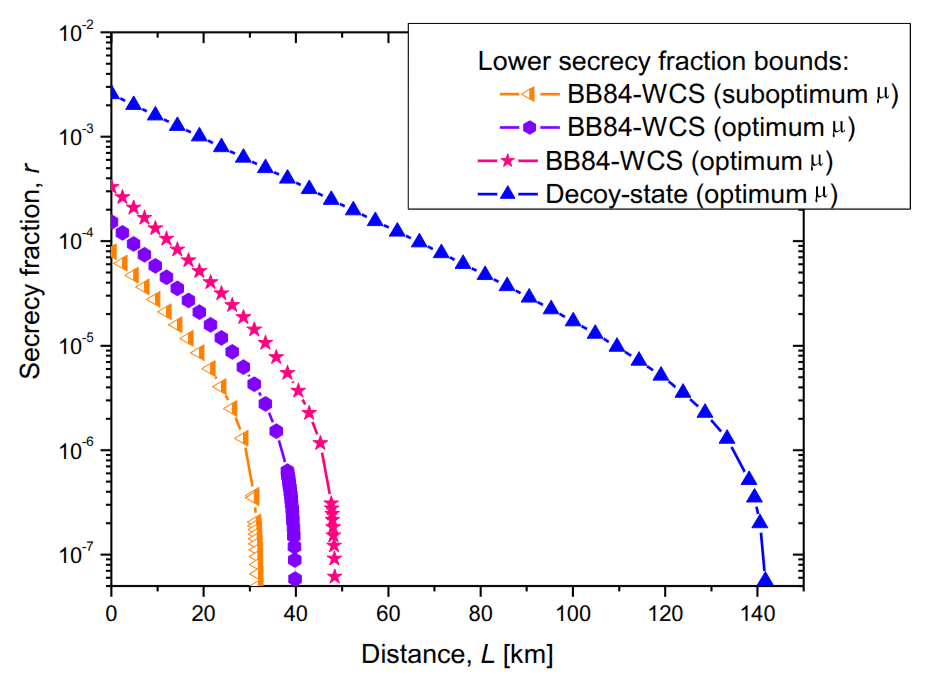
\includegraphics[width=0.8\textwidth]{chapters/figs/fig-6-11}
	\caption{کسر امنیت در مقابل مسافت ارسال برای پروتکل مبتنی بر حالت فریب و پروتکل \lr{BB84} مبتنی بر حالت همدوس ضعیف.}
	\label{fig:6-11}
\end{figure}


\section{پروتکل‌های توزیع کلید کوانتومی مستقل از دستگاه اندازه‌گیری}
\label{sec:6-7}
هرگونه اختلاف در پارامترهای دستگاه‌ها نسبت به فرضیات در نظر گرفته شده در پروتکل‌های \lr{QKD}، می‌تواند توسط مهاجمان از طریق حملات کانال جانبی و هک کوانتومی \cite{54,55,56,57,58} برای به مخاطره انداختن امنیت پروتکل‌های مربوطه مورد بهره‌برداری قرار گیرد. یکی از راه‌های حل این مشکل، ابداع روش‌های مختلف برای غلبه بر حملات شناخته‌شده‌ی کانال جانبی یا هک کوانتومی است. متأسفانه، شنودگر همیشه می‌تواند حملات پیچیده‌تری را طراحی کند. استراتژی دیگر و موثرتر، ابداع پروتکل‌های جدیدی است که در آن‌ها کمترین فرضیات درباره دستگاه‌های مورد استفاده در پروتکل در نظر گرفته شده باشد. یکی از این پروتکل‌ها با عنوان \lr{QKD} مستقل از دستگاه\LTRfootnote{Device-independent QKD (DI-QKD)} (\lr{DI-QKD}) شناخته می‌شود \cite{74,75,76,77} که در آن آمار آشکارسازی برای ایمن‌سازی کلید، بدون در نظر گرفتن هیچ فرضی در مورد عملکرد دستگاه‌ها تعیین شده است. در پروتکل‌های \lr{MDI-QKD}\LTRfootnote{Measurement-device-independent QKD (MDI-QKD)}، چارلی اندازه‌گیری‌های حالت بل (\lr{BSM}) را انجام داده و نتایج را اعلام می‌کند؛ به همین دلیل ابتدا به شرح \lr{BSM}ها می‌پردازیم.

\subsection{اندازه‌گیری‌های حالت بل فوتونی}
\label{subsec:6-7-1}
اندازه‌گیری‌های حالت بل\LTRfootnote{Bell state measurements (BSMs)} (\lr{BSM}) نقش کلیدی در محاسبات و ارتباطات کوانتومی فوتونی، از جمله دورنوردی کوانتومی \cite{78}، کدگذاری فوق‌فشرده\LTRfootnote{Superdense coding} \cite{79}، جابه‌جایی کوانتومی\LTRfootnote{Quantum swapping} \cite{80}، تکرارکننده‌های کوانتومی\LTRfootnote{Quantum repeaters} \cite{81} و \lr{QKD} \cite{82,83,84} ایفا می‌کنند. یک \lr{BSM} کامل نشان‌دهنده تصویر کردن هر حالتِ دوفوتونی بر حالت‌های بل بیشینه درهم‌تنیده\LTRfootnote{Maximally entangled Bell states} است که به‌صورت زیر تعریف می‌شوند:
\begin{equation}
	|\psi^{\pm}\rangle = \frac{1}{\sqrt{2}} (|01\rangle \pm |10\rangle); \quad |\phi^{\pm}\rangle = \frac{1}{\sqrt{2}} (|00\rangle \pm |11\rangle)
	\label{eq:6-45}
\end{equation}
متأسفانه، دستیابی به \lr{BSM} کامل تنها با استفاده از اپتیک خطی\LTRfootnote{Linear optics} و بدون فوتون‌های کمکی\LTRfootnote{Auxiliary photons} غیرممکن است. در مرجع \cite{85} نشان داده شده است که احتمال \lr{BSM} موفقیت‌آمیز برای دو فوتون که در حالت‌های ورودی کاملاً مخلوط\LTRfootnote{Complete mixed input states} هستند، به ۵۰٪ محدود می‌شود. رویکرد متداول برای تحلیل حالت بل، استفاده از یک \lr{BS} ۵۰:۵۰ و متعاقب آن استفاده از \lr{SPD}ها برای امکان تمایز حالت‌های متعامد است. به‌عنوان نمونه، چیدمان انجام \lr{BSM} روی حالت‌های قطبش در شکل \ref{fig:6-12} ارائه شده است. حالت‌های گسیل‌شده توسط آلیس و باب به‌ترتیب با عملگرهای چگالی $\rho_A$ و $\rho_B$ نشان داده می‌شوند. هنگامی که فوتون‌ها در ورودی‌های یک و دوِ \lr{BS} دارای قطبش یکسانی باشند، یعنی $|HH\rangle = |00\rangle$ یا $|VV\rangle = |11\rangle$، بر اساس اثر هونگ-او-ماندل\LTRfootnote{Hong-Ou-Mandel (HOM) effect} (\lr{HOM}) \cite{2,86,87}، آن‌ها به‌طور هم‌زمان در هر یک از پورت‌های خروجی ۳ یا ۴ ظاهر می‌شوند و حالت‌های بل $|\phi^{\pm}\rangle$ به‌صورت زیر تبدیل می‌شوند:
\begin{equation}
	|\phi^{\pm}\rangle = \frac{1}{\sqrt{2}} (|00\rangle_{12} \pm |11\rangle_{12}) \xrightarrow{BS} |\phi_{\text{out}}\rangle = \frac{1}{\sqrt{2}} (|00\rangle_{33} + |00\rangle_{44} \pm |11\rangle_{33} \pm |11\rangle_{44})
	\label{eq:6-46}
\end{equation}
و به‌وضوح توسط تقسیم‌کننده‌های پرتو قطبشی\LTRfootnote{Polarizing beam splitters (PBSs)} (\lr{PBS}) مربوطه قابل تمایز نیستند.

\begin{figure}[ht]
	\centering
	 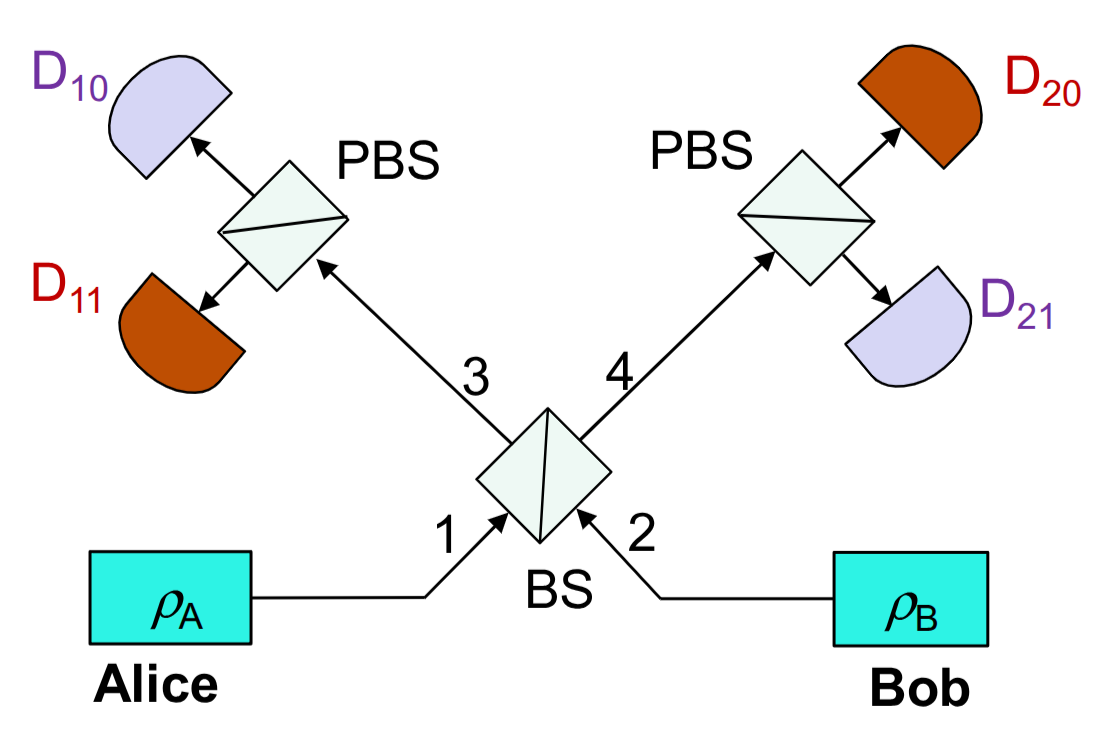
\includegraphics[width=0.8\textwidth]{chapters/figs/fig-6-12}
	\caption{تصویرسازی چیدمان برای انجام اندازه‌گیری‌های حالت بل روی حالت‌های قطبش.}
	\label{fig:6-12}
\end{figure}

از سوی دیگر، وقتی فوتون‌ها در پورت‌های ورودی یک و دوِ \lr{BS} دارای قطبش‌های متفاوتی باشند، می‌توانند از یک پورت خروجی یکسان یا پورت‌های متفاوت خارج شوند. هنگامی که هر دو فوتون از پورت خروجی ۳ خارج شوند، پس از \lr{PBS}، آشکارسازهای $D_{10}$ و $D_{11}$ به‌طور هم‌زمان کلیک می‌کنند. هنگامی که هر دو فوتون از پورت خروجی ۴ خارج شوند، پس از \lr{PBS}، آشکارسازهای $D_{20}$ و $D_{21}$ به‌طور هم‌زمان کلیک می‌کنند. زمانی که فوتون‌های ورودی با قطبش‌های متفاوت از پورت‌های متفاوتی خارج شوند، دو گزینه وجود دارد: وقتی فوتون افقی از پورت ۳ و فوتون عمودی از پورت ۴ خارج شود، $D_{11}$ و $D_{20}$ به‌طور هم‌زمان کلیک می‌کنند. در نهایت، وقتی فوتون افقی از پورت ۴ و فوتون عمودی از پورت ۳ خارج شود، $D_{10}$ و $D_{21}$ به‌طور هم‌زمان کلیک می‌کنند. با توجه به اینکه حالت‌های بل $|\psi^{\pm}\rangle$ (توسط \lr{BS}) به‌صورت زیر تبدیل می‌شوند:
\begin{equation}
	\begin{aligned}
		|\psi^+\rangle = \frac{1}{\sqrt{2}} (|01\rangle_{12} + |10\rangle_{12}) \xrightarrow{BS} |\psi_{\text{out}}^+\rangle = \frac{1}{\sqrt{2}} (|01\rangle_{33} + |10\rangle_{44}) \\
		|\psi^-\rangle = \frac{1}{\sqrt{2}} (|01\rangle_{12} - |10\rangle_{12}) \xrightarrow{BS} |\psi_{\text{out}}^-\rangle = \frac{1}{\sqrt{2}} (|01\rangle_{34} - |10\rangle_{34})
	\end{aligned}
	\label{eq:6-47}
\end{equation}
آن‌ها توسط \lr{PBS}ها و \lr{SPD}ها قابل تمایز هستند. به‌وضوح، بر اساس بحث بالا نتیجه می‌گیریم که تصویر شدن روی $|\psi^+\rangle$ زمانی رخ می‌دهد که هر دو \lr{SPD} بعد از هر یک از دو \lr{PBS} به‌طور هم‌زمان کلیک کنند. به عبارت دیگر، وقتی یا $D_{10}$ و $D_{11}$ و یا $D_{20}$ و $D_{21}$ به‌طور هم‌زمان کلیک کنند، تصویر شدن روی $|\psi^+\rangle$ شناسایی می‌شود. به‌طور مشابه، وقتی یا $D_{10}$ و $D_{21}$ و یا $D_{20}$ و $D_{11}$ به‌طور هم‌زمان کلیک کنند، تصویر شدن روی حالت $|\psi^-\rangle$ شناسایی می‌شود. در نتیجه، هنگام استفاده از \lr{SPD}های ایده‌آل، بازدهی \lr{BSM} برابر با $1/2$ است. اگر \lr{SPD}ها دارای بازدهی آشکارسازی غیرایده‌آل $\eta$ باشند، بازدهی \lr{BSM} برابر با $0.5\eta^2$ خواهد بود.

درجه آزادی دیگری که به‌طور گسترده برای کدگذاری حالت‌های کوانتومی استفاده می‌شود، درجه آزادی بازه زمانی\LTRfootnote{Time-bin} است. برای ارتباطات کوانتومی دوبعدی، فوتون را می‌توان به‌صورت برهم‌نهی از حالت زود\LTRfootnote{Early-state} (نشان‌ داده شده با $|0\rangle$) و حالت دیر\LTRfootnote{Late-state} (نشان داده شده با $|1\rangle$) به‌صورت $|\chi\rangle = a|0\rangle + b|1\rangle$ با شرط $|a|^2 + |b|^2 = 1$ کدگذاری کرد. برای انجام \lr{BSM} می‌توان از چیدمان ارائه شده در شکل \ref{fig:6-13} استفاده کرد که علاوه بر \lr{BS} تنها به دو \lr{SPD} نیاز دارد. مشابه قطبش، حالت‌های بل توسط رابطه \eqref{eq:6-45} اما با کِت‌های پایه متفاوت تعریف می‌شوند. باز هم، وقتی دو فوتون در یک زمان واحد به پورت‌های ورودی \lr{BS} می‌رسند، طبق اثر \lr{HOM} از یک پورت خروجی یکسان خارج می‌شوند و ما نمی‌توانیم حالت‌های $|\phi^{\pm}\rangle$ را متمایز کنیم. از سوی دیگر، تصویر شدن روی $|\psi^+\rangle$ زمانی شناسایی می‌شود که هر یک از آشکارسازها در بازه‌های زمانی زود و دیر کلیک ثبت کنند. به‌طور مشابه، تصویر شدن روی $|\psi^-\rangle$ زمانی رخ می‌دهد که هر یک از آشکارسازهای $D_1$ و $D_2$ یا $D_2$ و $D_1$ در بازه‌های زمانی متوالی (زود-دیر) کلیک کنند.

\begin{figure}[ht]
	\centering
	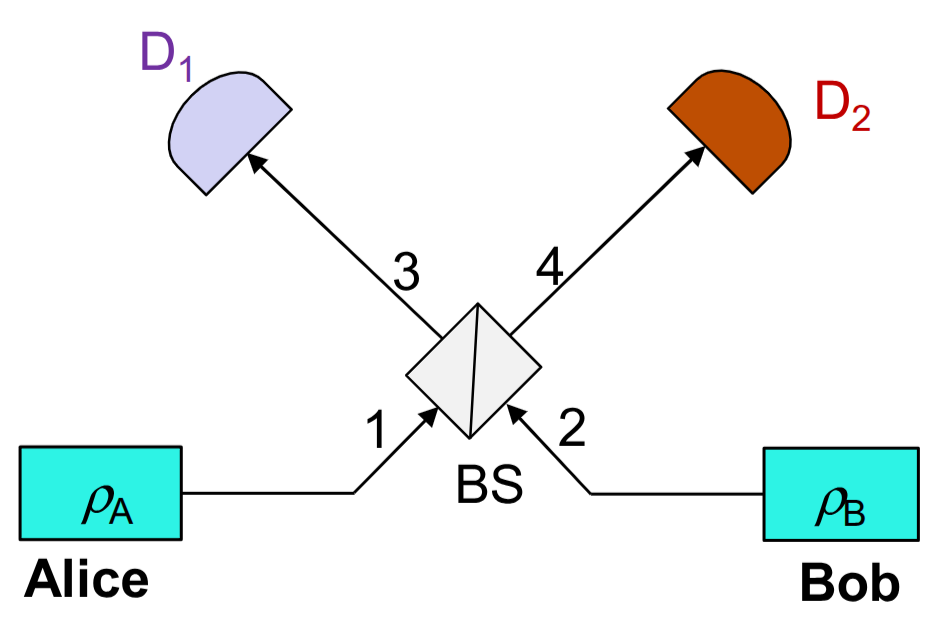
\includegraphics[width=0.8\textwidth]{chapters/figs/fig-6-13}
	\caption{تصویرسازی چیدمان برای انجام اندازه‌گیری‌های حالت بل روی حالت‌های بازه زمانی.}
	\label{fig:6-13}
\end{figure}

\subsection{شرح پروتکل توزیع کلید کوانتومی مستقل از دستگاه اندازه‌گیری}
\label{subsec:6-7-2}
در پروتکل‌های \lr{MDI-QKD} \cite{82,88,89,90,91}، آلیس و باب از طریق یک کانال کوانتومی، مانند یک پیوند نوری فضای آزاد (\lr{FSO}) یا فیبر نوری، به یک شخص ثالث به نام چارلی متصل می‌شوند. همان‌طور که در شکل \ref{fig:6-14} برای پروتکل \lr{MDI-QKD} مبتنی بر قطبش تصویر شده است، آشکارسازهای \lr{SPD} در سمت چارلی قرار دارند.

آلیس و باب می‌توانند از منابع تک‌فوتونی یا منابع \lr{WCS} استفاده کنند و به‌طور تصادفی یکی از چهار حالت $|0\rangle$، $|1\rangle$، $|+\rangle$ یا $|-\rangle$ را با کمک یک مدولاتور قطبش\LTRfootnote{Polarization modulator (PolM)} (\lr{PolM}) که بسیار شبیه به مدولاتور مورد استفاده در پروتکل \lr{BB84} است، برای ارسال به چارلی انتخاب کنند. از یک مدولاتور شدت\LTRfootnote{Intensity modulator} برای اعمال حالت‌های فریب مختلف استفاده می‌شود. چارلی اساساً می‌تواند خودِ ایو باشد. او \lr{BSM} جزئی را با کمک یک \lr{BS}، دو \lr{PBS} و چهار \lr{SPD} مطابق شکل \ref{fig:6-14} انجام می‌دهد و رویدادهایی را اعلام می‌کند که در آن‌ها نتیجه اندازه‌گیری منجر به یکی از دو حالت $|\psi^+\rangle = (|01\rangle + |10\rangle)/\sqrt{2}$ یا $|\psi^-\rangle = (|01\rangle - |10\rangle)/\sqrt{2}$ شده باشد. چارلی همچنین نتایج \lr{BSM} را فاش می‌کند. با توجه به اینکه اندازه‌گیری‌های حالت بل چارلی تنها برای بررسی توازن (پاریته) بیت‌های آلیس و باب استفاده می‌شوند، این اندازه‌گیری‌ها هیچ اطلاعاتی در مورد خودِ بیت‌های منفرد فاش نخواهند کرد \cite{88}.

\begin{figure}[ht]
	\centering
	 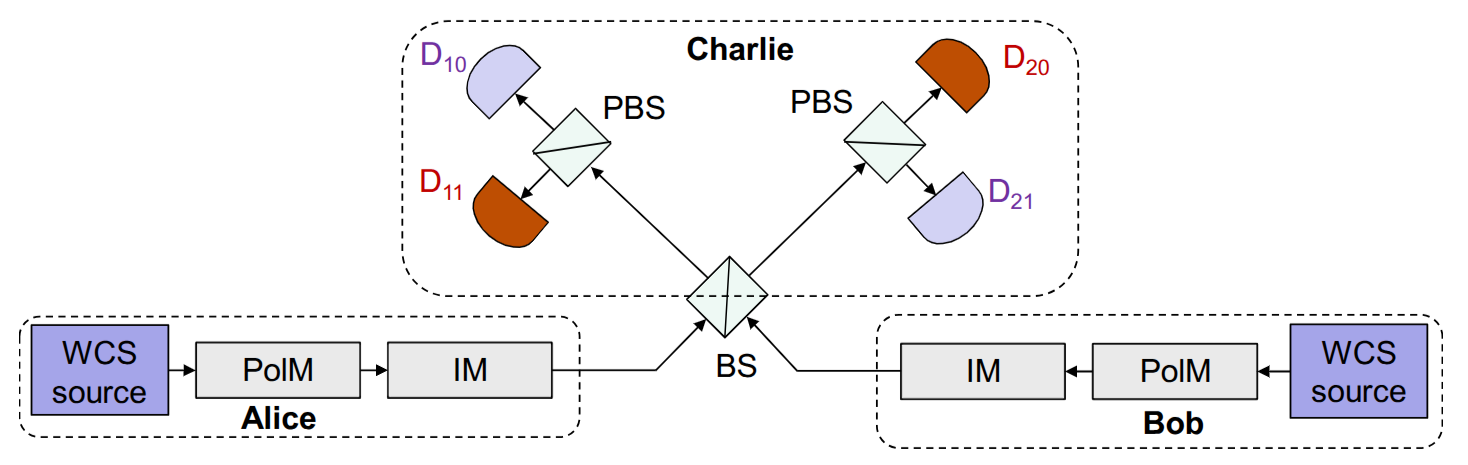
\includegraphics[width=0.8\textwidth]{chapters/figs/fig-6-14}
	\caption{پیکربندی سیستم توزیع کلید کوانتومی مستقل از دستگاه اندازه‌گیری مبتنی بر حالت قطبش.}
	\label{fig:6-14}
\end{figure}

یک \lr{BSM} موفق متناظر با مشاهداتی است که در آن دقیقاً دو آشکارساز (با قطبش‌های متعامد) به‌صورت زیر تحریک شوند:
\begin{itemize}
	\item کلیک هم‌زمان آشکارسازهای $D_{10}$ و $D_{21}$ حالت بل $|\psi^-\rangle$ را شناسایی می‌کند.
	\item از سوی دیگر، کلیک هم‌زمان آشکارسازهای $D_{11}$ و $D_{20}$ حالت بل $|\psi^+\rangle$ را شناسایی می‌کند.
\end{itemize}
سایر الگوهای آشکارسازی مربوط به حالت‌های $|\phi^{\pm}\rangle$ هستند که با \lr{SPD}ها قابل تمایز نیستند و بنابراین موفقیت‌آمیز تلقی نشده و از بررسی کنار گذاشته می‌شوند. به‌وضوح، بر اساس شرح فوق نتیجه می‌گیریم که پروتکل \lr{MDI-QKD} تعمیمی از هر دو پروتکل \lr{QKD} مبتنی بر \lr{EPR} (تبدیل شده به طرح آماده‌سازی-و-اندازه‌گیری) و پروتکل مبتنی بر حالت فریب است. آلیس و باب با مقایسه بخشی از دنباله‌های خود می‌توانند صداقت چارلی را تأیید کنند.

اکنون یک پیاده‌سازی ممکن برای \lr{PolM}، یعنی پیکربندی رمزگذار \lr{BB84} مبتنی بر حالت فریب را شرح می‌دهیم که در شکل \ref{fig:6-15} ارائه شده است. سیگنال باریکه لیزر توسط یک کوپلر ۱:۴ به چهار شاخه تقسیم می‌شود که هر شاخه شامل یک کنترل‌کننده قطبش برای اعمال حالت‌های قطبش $|0\rangle$، $|1\rangle$، $|+\rangle$ و $|-\rangle$ است. با کمک یک سوئیچ نوری فضایی\LTRfootnote{Optical space switch} ۴:۱، حالت قطبش ارسالی به چارلی را به‌طور تصادفی انتخاب می‌کنیم. برای این منظور، استفاده از سوئیچ‌هایی با سوئیچینگ الکترواپتیکی مطلوب است (مانند آنچه در مراجع \cite{92, 93} گزارش شده است)، زیرا در این سوئیچ‌ها حالت سوئیچینگ را می‌توان در عرض چند نانوثانیه تغییر داد. مدولاتور فاز در خروجی برای انجام تصادفی‌سازی فاز\LTRfootnote{Phase randomization} حالت همدوس $|\alpha\rangle = \exp(-|\alpha|^2/2) \sum \alpha^n |n\rangle / \sqrt{n!}$ به‌صورت زیر به کار می‌رود:
\begin{equation}
	\begin{aligned}
		\frac{1}{2\pi} \int_{0}^{2\pi} |\alpha e^{j\omega}\rangle \langle \alpha e^{j\omega} | d\omega &= \frac{1}{2\pi} \sum_{n=0}^{\infty} \sum_{m=0}^{\infty} \frac{|\alpha|^{m+n}}{\sqrt{m!n!}} e^{-|\alpha|^2} |n\rangle\langle m| \underbrace{\int_{0}^{2\pi} e^{j(n-m)\omega} d\omega}_{\delta_{nm}} \\
		&= \sum_{n=0}^{\infty} \frac{|\alpha|^{2n}}{n!} e^{-|\alpha|^2} |n\rangle\langle n| = \sum_{n=0}^{\infty} \frac{\mu^n}{n!} e^{-\mu} |n\rangle\langle n|; \quad \mu = |\alpha|^2
	\end{aligned}
	\label{eq:6-48}
\end{equation}
که در آن $\mu = |\alpha|^2$ میانگین تعداد فوتون در هر پالس است. سپس از یک تضعیف‌کننده نوری متغیر برای کاهش میانگین تعداد فوتون تا سطح کوانتومی استفاده می‌شود. سایر پیکربندی‌های \lr{PolM} نیز می‌توانند استفاده شوند، مانند آنچه در مرجع \cite{88} با استفاده از چهار دیود لیزری شرح داده شده است. آلیس و باب سپس از طریق یک کانال کلاسیک احرازهویت‌شده و بدون نویز، اطلاعات مربوط به پایه‌های استفاده شده را مبادله می‌کنند: پایه $Z$ شامل حالت‌های $|0\rangle$ و $|1\rangle$ (پایه محاسباتی) یا پایه $X$ شامل حالت‌های $|+\rangle$ و $|-\rangle$ (پایه قطری). پس از آن، آلیس و باب تنها رویدادهایی را نگه می‌دارند که در آن‌ها از پایه یکسانی استفاده کرده‌اند و در عین حال چارلی حالت‌های \lr{BSM} یعنی $|\psi^-\rangle$ یا $|\psi^+\rangle$ را اعلام کرده است. یکی از آن‌ها (مثلاً باب) بیت‌های ارسالی را وارونه (فلیپ) می‌کند، مگر زمانی که هر دو از پایه قطری استفاده کرده باشند و چارلی حالت $|\psi^+\rangle$ را اعلام کرده باشد. سایر رویدادها کنار گذاشته می‌شوند.

\begin{figure}[ht]
	\centering
	 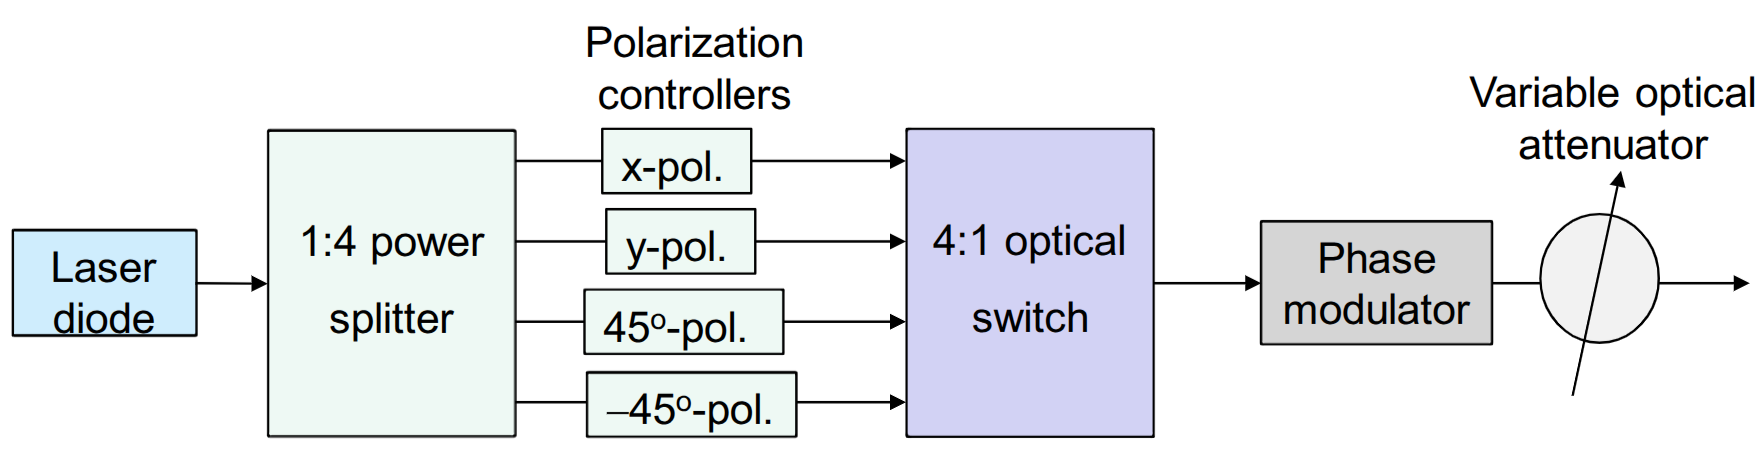
\includegraphics[width=0.8\textwidth]{chapters/figs/fig-6-15}
	\caption{پیکربندی رمزگذار \lr{BB84} (\lr{PolM}) مبتنی بر حالت فریب.}
	\label{fig:6-15}
\end{figure}





علاوه بر این، کلید-$X$ از آن بیت‌هایی تشکیل می‌شود که آلیس و باب فوتون‌های خود را در پایه $X$ (پایه قطری) آماده کرده بودند. نرخ خطا در این بیت‌ها برای محدود کردن اطلاعات کسب شده توسط ایو استفاده می‌شود. سپس، آلیس و باب کلید-$Z$ را از آن بیت‌هایی تشکیل می‌دهند که برای آن‌ها هر دو از پایه $Z$ (پایه محاسباتی) استفاده کرده‌اند. در نهایت، آن‌ها مصالحه اطلاعات و تقویت حریم خصوصی را روی کلید-$Z$ انجام می‌دهند تا به کلید مخفی دست یابند.

پروتکل \lr{MDI-QKD} علاوه بر حساس نبودن به \lr{SPD}های استفاده شده توسط چارلی، امکان اتصال چندین شرکت‌کننده را در یک شبکه \lr{QKD} ستاره‌ای\LTRfootnote{Star-like QKD network} فراهم می‌کند که در آن چارلی در مرکز (به‌عنوان یک هاب\LTRfootnote{Hub}) قرار دارد \cite{94, 95}. در این شبکه \lr{QKD} که در شکل \ref{fig:6-16} نشان داده شده است، گران‌ترین تجهیزات (\lr{SPD}ها) بین چندین کاربر به اشتراک گذاشته می‌شوند و شبکه \lr{QKD} را می‌توان به راحتی و بدون ایجاد اختلال برای سایر کاربران ارتقا داد. با کمک یک سوئیچ نوری $N:2$، هر دو کاربر می‌توانند در پروتکل \lr{MDI-QKD} برای تبادل کلیدهای امن شرکت کنند.

\begin{figure}[ht]
	\centering
	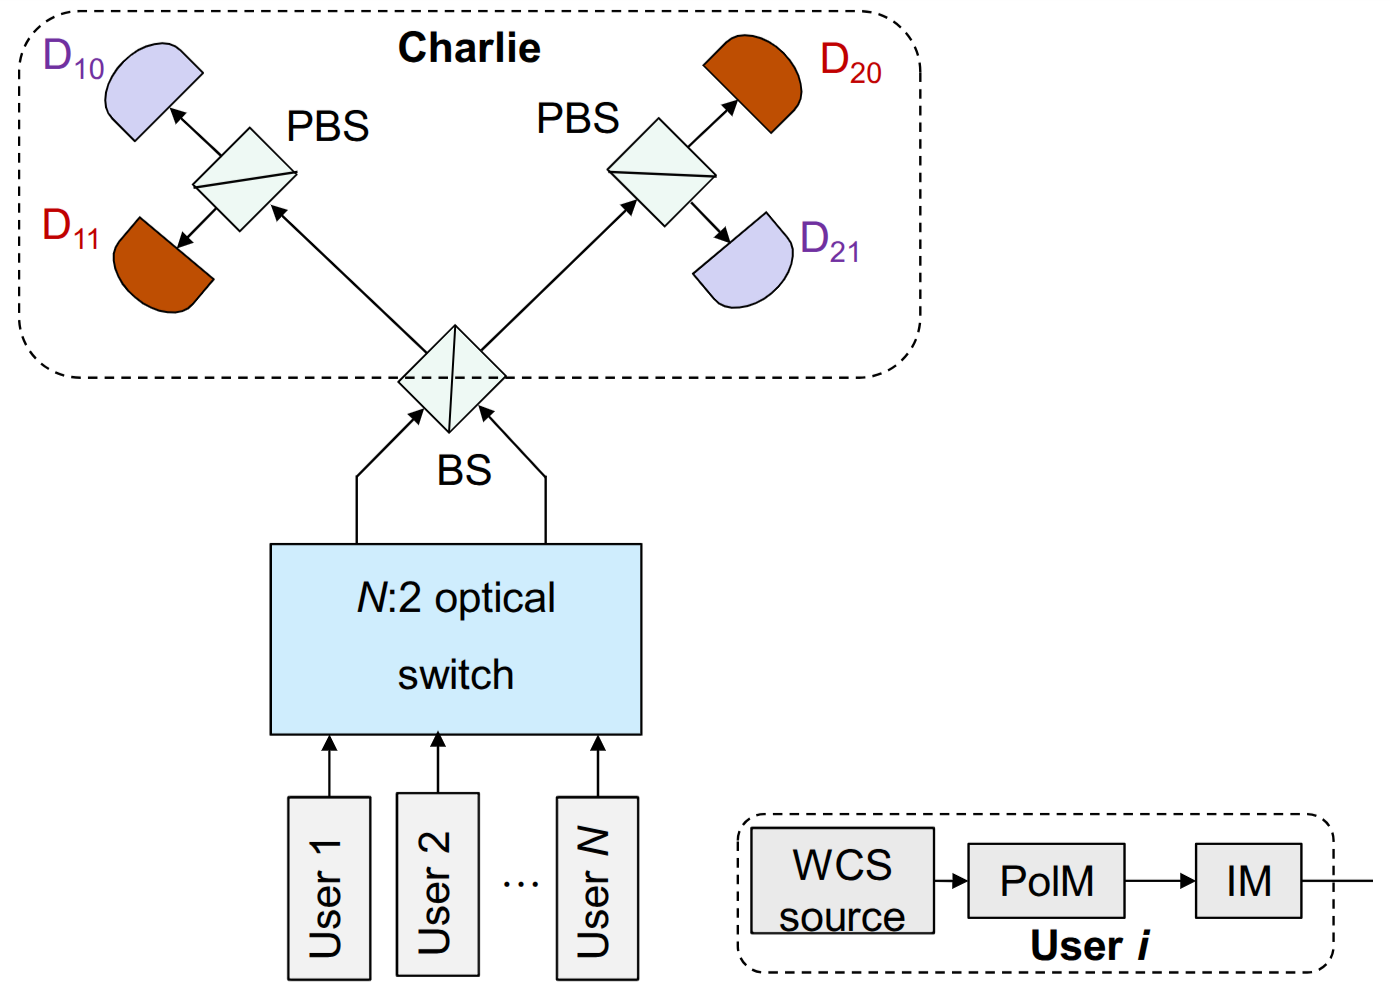
\includegraphics[width=0.7\textwidth]{chapters/figs/fig-6-16}
	\caption{پیکربندی شبکه توزیع کلید کوانتومی ستاره‌ای مبتنی بر \lr{MDI-QKD}.}
	\label{fig:6-16}
\end{figure}

\subsubsection{پروتکل توزیع کلید کوانتومی مستقل از دستگاه اندازه‌گیری مبتنی بر کدگذاری فاز-زمان}
\label{subsec:6-7-3}
حالت‌های پایه کدگذاری فاز-زمان برای پروتکل \lr{BB84} ($N=2$) در شکل \ref{fig:6-17} ارائه شده‌اند. پایه زمانی متناظر با پایه محاسباتی $\{|0\rangle, |1\rangle\}$ است، در حالی که پایه فازی متناظر با پایه قطری $\{|+\rangle, |-\rangle\}$ می‌باشد. پالس در یک بازه زمانی\LTRfootnote{Time bin} با مدت‌زمان $\tau = T/2$ متمرکز شده است. پایه زمانی مشابه \lr{PPM} است. حالتی که در آن فوتون در اولین بازه زمانی قرار می‌گیرد (حالت زود\LTRfootnote{Early state})، با $|0\rangle = |e\rangle$ نشان داده می‌شود، در حالی که حالتی که در آن فوتون در دومین بازه زمانی قرار می‌گیرد (حالت دیر\LTRfootnote{Late state})، با $|1\rangle = |l\rangle$ نشان داده می‌شود. حالت‌های فاز-زمان به‌صورت $|+\rangle = (|0\rangle + |1\rangle)/\sqrt{2}$ و $|-\rangle = (|0\rangle - |1\rangle)/\sqrt{2}$ تعریف می‌شوند. آلیس به‌طور تصادفی یا پایه زمانی یا پایه فازی را انتخاب کرده و متعاقب آن به‌طور تصادفی حالت پایه را انتخاب می‌کند. مقدار منطقی $0$ توسط $|0\rangle$ و $|+\rangle$ بازنمایی می‌شود؛ در حالی که مقدار منطقی $1$ توسط $|1\rangle$ و $|-\rangle$ نشان داده می‌شود. آلیس و باب به‌طور تصادفی یکی از چهار حالت $|0\rangle, |1\rangle, |+\rangle, |-\rangle$ را برای ارسال به چارلی انتخاب می‌کنند. چارلی \lr{BSM} جزئی را با کمک یک \lr{BS} ۵۰:۵۰ و دو \lr{SPD} مطابق شکل \ref{fig:6-18} انجام می‌دهد و رویدادهایی را اعلام می‌کند که در آن‌ها نتیجه اندازه‌گیری منجر به یکی از دو حالت $|\psi^+\rangle = (|01\rangle + |10\rangle)/\sqrt{2}$ یا $|\psi^-\rangle = (|01\rangle - |10\rangle)/\sqrt{2}$ شده باشد.



\begin{figure}[ht]
	\centering
	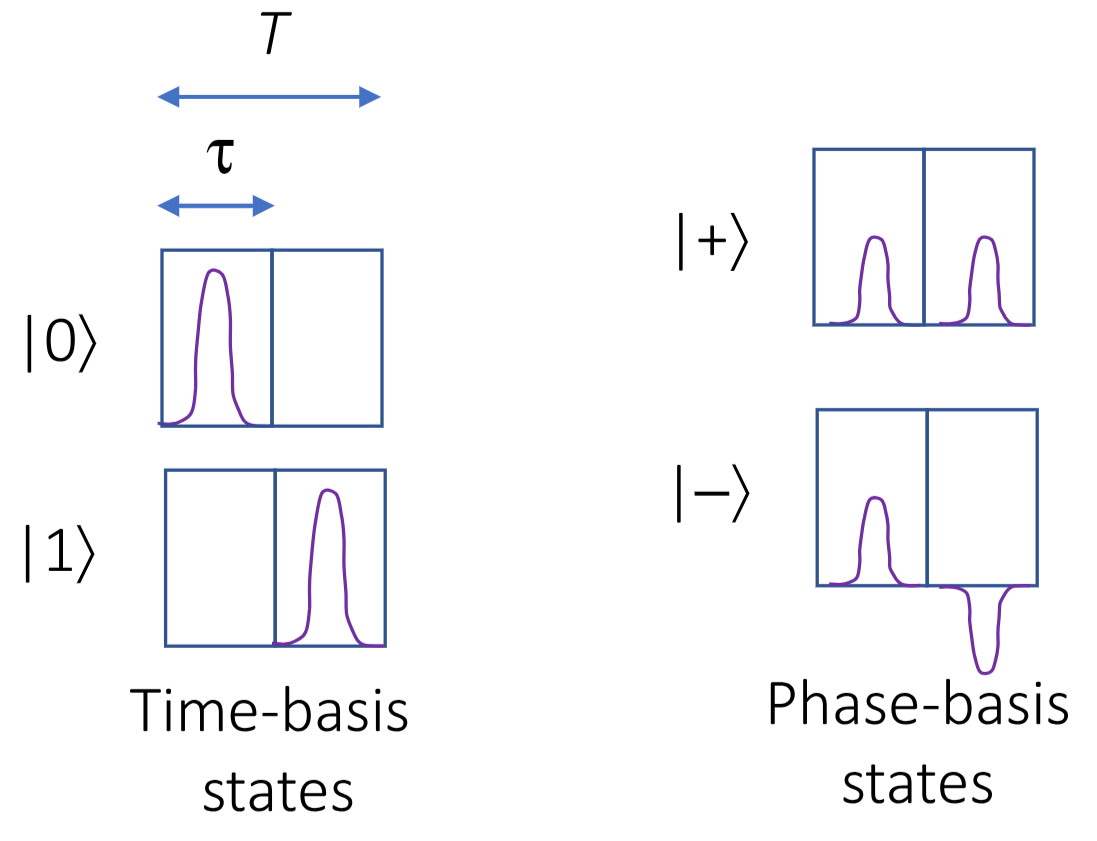
\includegraphics[width=0.5\textwidth]{chapters/figs/fig-6-17}
	\caption{حالت‌های پایه زمانی و پایه فازی مورد استفاده در کدگذاری فاز-زمان برای پروتکل \lr{BB84}.}
	\label{fig:6-17}
\end{figure}

چارلی همچنین نتیجه \lr{BSM} را فاش می‌کند. یک \lr{BSM} موفق متناظر با مشاهداتی است که در آن‌ها \lr{SPD}ها به‌صورت زیر تحریک شوند:
\begin{itemize}
	\item دو کلیک متوالی (هر دو در بازه‌های زمانی زود و دیر) روی یکی از \lr{SPD}ها، حالت بل $|\psi^-\rangle$ را شناسایی می‌کند.
	\item از سوی دیگر، زمانی که یک \lr{SPD} حضور فوتون را در بازه زمانی زود و دیگری در بازه زمانی دیر آشکار کند، حالت بل $|\psi^+\rangle$ را شناسایی می‌کنیم.
	\item سایر الگوهای آشکارسازی مربوط به حالت‌های $|\phi^{\pm}\rangle$ هستند و از بررسی کنار گذاشته می‌شوند.
\end{itemize}
بقیه پروتکل مشابه پروتکل \lr{MDI-QKD} مبتنی بر حالت قطبش است. برای پیاده‌سازی رمزگذار فاز-زمان، آلیس و باب می‌توانند یا از مدولاتور قطبی الکترواپتیکی، متشکل از اتصال پیاپی یک مدولاتور دامنه و یک مدولاتور فاز (مطابق شکل \ref{fig:6-18}) استفاده کنند، و یا به‌صورت جایگزین، یک مدولاتور \lr{I/Q} الکترواپتیکی را به کار گیرند \cite{46, 96}. مدولاتور دامنه (مدولاتور ماخ-زندر) برای شکل‌دهی پالس و مدولاتور فاز برای اعمال جابه‌جایی فاز مطلوب مطابق با حالت‌های پایه فازی استفاده می‌شود (شکل \ref{fig:6-17} را ببینید). از \lr{AWG}ها می‌توان برای تولید شکل‌موج‌های \lr{RF} متناظر بر حسب نیاز استفاده کرد. \lr{VOA}ها نیز برای تضعیف باریکه مدوله‌شده تا سطح تک‌فوتون به کار می‌روند. برای عملکرد صحیح، \lr{AWG}ها باید هم‌زمان\LTRfootnote{Synchronized} باشند. علاوه بر این، دیودهای لیزر موج پیوسته\LTRfootnote{Continuous-wave (CW)} مورد استفاده توسط آلیس و باب باید قفل فرکانسی\LTRfootnote{Frequency locked} شده باشند. در نهایت، فوتون‌های ورودی به \lr{BSM} (از سوی آلیس و باب) باید قطبش یکسانی داشته باشند.

\begin{figure}[ht]
	\centering
	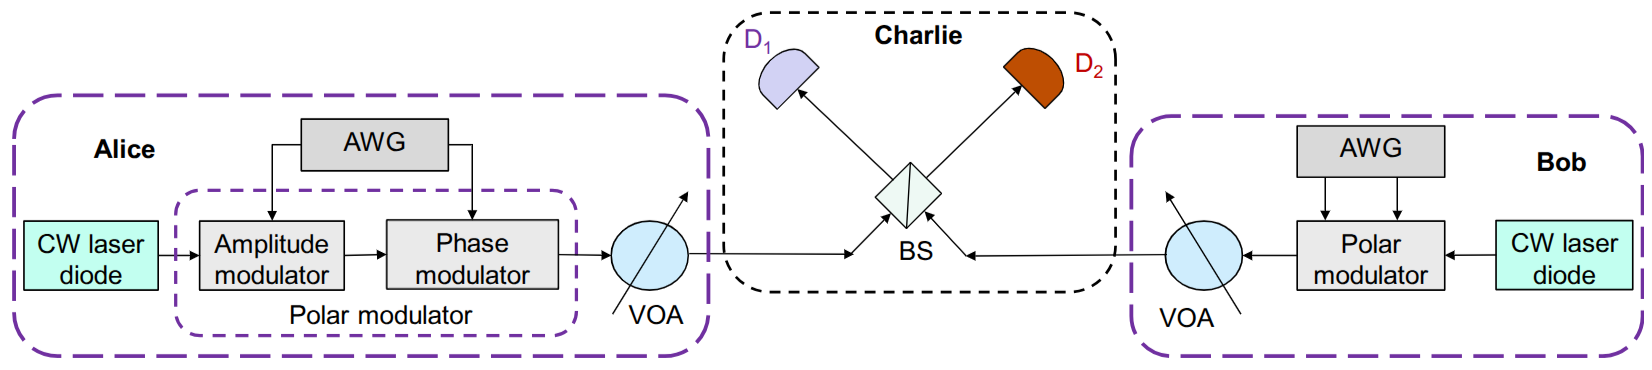
\includegraphics[width=\textwidth]{chapters/figs/fig-6-18}
	\caption{پیکربندی سیستم توزیع کلید کوانتومی مستقل از دستگاه اندازه‌گیری مبتنی بر کدگذاری فاز-زمان.}
	\label{fig:6-18}
\end{figure}

\subsubsection{کسر امنیت پروتکل‌های توزیع کلید کوانتومی مستقل از دستگاه اندازه‌گیری}
\label{subsec:6-7-4}
کسر مخفی پروتکل \lr{MDI-QKD}، زمانی که آلیس و باب هر دو از منابع تک‌فوتونی استفاده می‌کنند، مشابه پروتکل \lr{BB84} است:
\begin{equation}
	r = q(Z) [ 1 - h_2(e(X)) ] - q(Z) f_e h_2(e(Z))
	\label{eq:6-49}
\end{equation}
که در آن $q(Z)$ اکنون نشان‌دهنده احتمال نتیجه موفقیت‌آمیز \lr{BSM} («بهره») است. از سوی دیگر، زمانی که آلیس و باب هر دو از منابع \lr{WCS} استفاده می‌کنند، باید روش حالت فریب به کار گرفته شود تا کسر مخفی مطابق مرجع \cite{89} به‌صورت زیر تخمین زده شود:
\begin{equation}
	r = q(Z)_{11} [ 1 - h_2(e(X)_{11}) ] - q(Z)_{\mu\sigma} f_e h_2(e(Z)_{\mu\sigma})
	\label{eq:6-50}
\end{equation}
که در آن نمادگذاری‌های زیر را معرفی کردیم:
\begin{itemize}
	\item $q(Z)_{11}$ نشان‌دهنده احتمالی است که چارلی یک نتیجه موفقیت‌آمیز («بهره») را اعلام کند، در حالی که آلیس و باب هر کدام یک تک‌فوتون را در پایه $Z$ ارسال کرده‌اند.
	\item $e(X)_{11}$ نشان‌دهنده نرخ خطای فاز سیگنال‌های تک‌فوتونی است که هر دو در پایه $Z$ ارسال شده‌اند.
	\item $q(Z)_{\mu\sigma}$ نشان‌دهنده بهره در پایه $Z$ است، زمانی که آلیس حالت \lr{WCS} با شدت $\mu$ را برای چارلی ارسال می‌کند، در حالی که باب به‌طور هم‌زمان حالت \lr{WCS} با شدت $\sigma$ را می‌فرستد.
\end{itemize}
در معادله فوق، اطلاعات حذف شده از کلید نهایی در مرحله تقویت حریم خصوصی توسط جمله $q(Z)_{11} h_2(e(X)_{11})$ توصیف می‌شود. اطلاعات فاش شده توسط آلیس در مرحله مصالحه اطلاعات با جمله $q(Z)_{\mu\sigma} f_e h_2(e(Z)_{\mu\sigma})$ توصیف می‌گردد که در آن مانند قبل، $f_e$ ناکارآمدی تصحیح خطا ($f_e \geq 1$) است. نرخ‌های خطای $q(Z)_{11}$ و $e(X)_{11}$ را نمی‌توان به‌طور مستقیم اندازه‌گیری کرد، بلکه در عوض با به‌کارگیری رویکرد حالت فریب به شیوه‌ای مشابه آنچه در بخش قبل شرح داده شد، محدود می‌شوند.


\section{پروتکل‌های توزیع کلید کوانتومی میدان-دوقلو}
\label{sec:6-8}
کانال کوانتومی را می‌توان با گذردهی\LTRfootnote{Transmissivity} $T$ مشخص کرد که می‌توان آن را به عنوان احتمال ارسال موفقیت‌آمیز یک فوتون توسط کانال نیز تفسیر کرد. ظرفیت کلید-مخفی کانال کوانتومی می‌تواند به عنوان حد بالایی برای حداکثر نرخ کلید مخفی ممکن استفاده شود. در بسیاری از موارد، کران پیراندولا-لورنزا-اوتاویانی-بانکی\LTRfootnote{Pirandola-Laurenza-Ottaviani-Banchi (PLOB)} (\lr{PLOB}) روی نرخ کلید خطی استفاده می‌شود که طبق مرجع \cite{97} به‌صورت $r_{PLOB} = -\log_2(1-T)$ داده می‌شود. برای غلبه بر محدودیت نرخ-مسافت در پروتکل‌های \lr{DV-QKD}، تا همین اواخر دو رویکرد دنبال شده است: (الف) توسعه رله‌های کوانتومی\LTRfootnote{Quantum relays} \cite{98} و (ب) استفاده از رله‌های مورد اعتماد\LTRfootnote{Trusted relays} \cite{99}. متأسفانه، رله‌های کوانتومی نیازمند استفاده از حافظه‌های کوانتومی با زمان طولانی و تقطیر درهم‌تنیدگی\LTRfootnote{Entanglement distillation} با وفاداری بالا هستند که هنوز با فناوری فعلی دور از دسترس می‌باشند. از سوی دیگر، روش رله مورد اعتماد فرض می‌کند که رله بین دو کاربر قابل اعتماد است و تأیید این فرض در عمل دشوار است. رویکرد \lr{MDI-QKD} که در بخش قبل شرح داده شد، توانست گریزگاه‌های آشکارسازی\LTRfootnote{Detection loopholes} را ببندد و مسافت ارسال را افزایش دهد؛ با این حال، \lr{SKR} آن همچنان توسط وابستگی $O(T)$ در حد بالا محدود می‌شود.

اخیراً، \lr{QKD} میدان-دوقلو\LTRfootnote{Twin-field QKD (TF-QKD)} (\lr{TF-QKD}) برای غلبه بر محدودیت نرخ-مسافت پیشنهاد شده است \cite{100}. نویسندگان در مرجع \cite{100} نشان داده‌اند که حد بالای \lr{TF-QKD} با ریشه دوم گذردهی مقیاس‌بندی می‌شود، یعنی $r \approx O(\sqrt{T})$. در \lr{TF-QKD}، آلیس و باب یک جفت میدان نوری با فازهای تصادفی و کدگذاری فاز در پایه‌های $X$ و $Y$ در مقاصد دور تولید کرده و آن‌ها را برای چارلی (یا ایو) غیرقابل‌اعتماد ارسال می‌کنند که او سپس آشکارسازی تک‌فوتون را انجام می‌دهد. این طرح مزایای طرح \lr{MDI-QKD} مانند مصونیت در برابر حملات آشکارساز، تسهیم‌سازی\LTRfootnote{Multiplexing} \lr{SPD} و معماری شبکه ستاره‌ای را حفظ کرده و در عین حال بر کران \lr{PLOB} غلبه می‌کند. اثبات امنیت غیرمشروط در مرجع \cite{100} ارائه نشده بود، اما در مجموعه‌ای از مقالات ثابت شد که این طرح از امنیت غیرمشروط برخوردار است \cite{101,102,103,104}. طرح \lr{TF-QKD} را می‌توان به عنوان تعمیمی از هر دو مورد (۱) طرح \lr{MDI-QKD} مبتنی بر کدگذاری فاز-زمان نشان داده شده در شکل \ref{fig:6-18} و (۲) \lr{BB84} مبتنی بر کدگذاری فاز (بخش \ref{sec:6-4-4}) تفسیر کرد.

نویسندگان در مرجع \cite{104} نشان داده‌اند که طرح \lr{TF-QKD} را می‌توان به عنوان یک طرح \lr{MDI-QKD} خاص که در یک زیرفضای دوبعدی از حالت خلاء $|0\rangle$ و حالت تک‌فوتونی $|1\rangle$ پیاده‌سازی شده است تفسیر کرد (همان‌طور که در شکل \ref{fig:6-19} نشان داده شده است) که نشان‌دهنده یک مدل معادل برای \lr{TF-QKD} با منابع تک‌فوتونی و دیودهای لیزری است. با توجه به اینکه حالت خلاء نسبت به تلفات کانال حساس نیست، این حالت همیشه قابل آشکارسازی است، یعنی «عدم کلیک» به معنای آشکارسازی موفقیت‌آمیز حالت خلاء است. این بهبود در احتمال آشکارسازی حالت خلاء عملاً منجر به \lr{SKR} بالاتری نسبت به \lr{MDI-QKD} سنتی شده و کران نرخ کلید خطی را می‌شکند. پایه محاسباتی یا پایه $Z$ توسط $\{|0\rangle, |1\rangle\}$ تعریف می‌شود (که در آن $|0\rangle$ و $|1\rangle$ همان‌طور که در بالا ذکر شد، به‌ترتیب نشان‌دهنده حالت خلاء و تک‌فوتونی هستند). پایه $X$ (پایه قطری) توسط $\{ |+\rangle = (|0\rangle + |1\rangle)/\sqrt{2}, |-\rangle = (|0\rangle - |1\rangle)/\sqrt{2} \}$ تعریف می‌شود، در حالی که پایه $Y$ توسط $\{ |+j\rangle = (|0\rangle + j|1\rangle)/\sqrt{2}, |-j\rangle = (|0\rangle - j|1\rangle)/\sqrt{2} \}$ تعریف می‌گردد. حالت‌های بل نیز به شیوه‌ای مشابه قبل تعریف می‌شوند، یعنی $|\psi^{\pm}\rangle = (|01\rangle \pm |10\rangle)/\sqrt{2}$.

آلیس (باب) با کمک دومین سوئیچ نوری به‌طور تصادفی انتخاب می‌کند که از پایه $Z$ یا پایه $X/Y$ استفاده کند. وقتی پایه $Z$ انتخاب می‌شود، آلیس (باب) سوئیچ نوری اول را برای انتخاب تصادفی حالت خلاء $|0\rangle$ یا حالت تک‌فوتونی به کار می‌گیرد و حالت انتخاب شده از طریق یک کانال نوری (فیبر \lr{SMF} یا پیوند \lr{FSO}) به سمت چارلی ارسال می‌شود. وقتی شاخه پایه $X/Y$ انتخاب می‌شود، لیزر \lr{CW} حالت همدوس $|\alpha\rangle$ را تولید می‌کند که توسط \lr{VOA} تضعیف می‌شود تا حالت برهم‌نهی از خلاء و تک‌فوتون به‌دست آید، یعنی $|+\rangle = (|0\rangle + |1\rangle)/\sqrt{2}$. آلیس (باب) با کمک یک مدولاتور فاز به‌طور تصادفی یکی از چهار فاز را از مجموعه $\{0, \pi, \pi/2, 3\pi/2\}$ انتخاب می‌کند. به این ترتیب، هر دو حالت برای پایه $X$ و پایه $Y$ به‌صورت تصادفی انتخاب می‌شوند. (به‌صورت جایگزین، به جای دو سوئیچ نوری ۲:۱، می‌توان از یک سوئیچ نوری ۴:۱ استفاده کرد).

\begin{figure}[ht]
	\centering
	 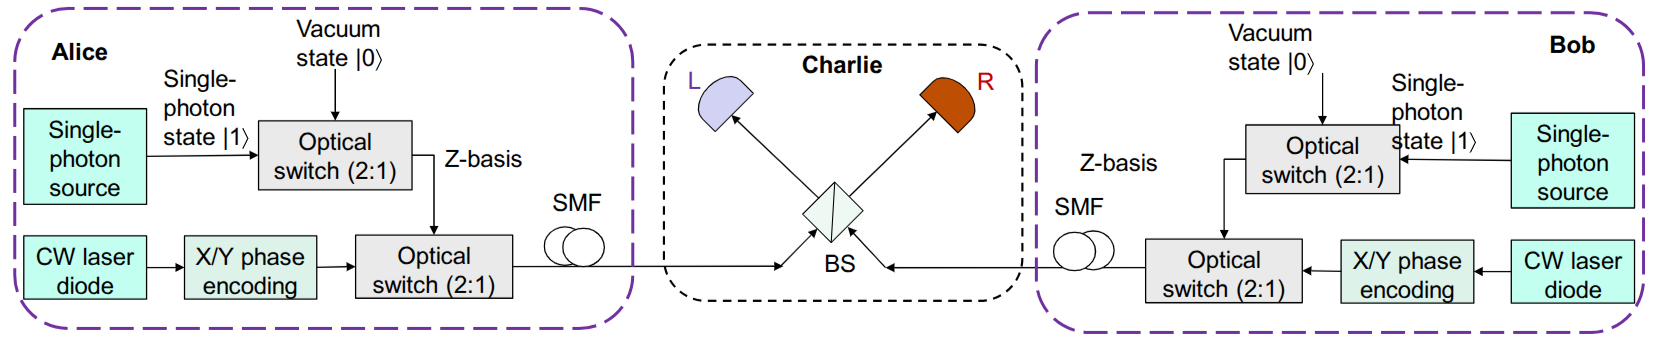
\includegraphics[width=\textwidth]{chapters/figs/fig-6-19}
	\caption{سیستم مفهومی توزیع کلید کوانتومی میدان-دوقلو با منابع تک‌فوتونی و لیزر موج پیوسته.}
	\label{fig:6-19}
\end{figure}

چارلی اندازه‌گیری‌های \lr{BSM} را انجام می‌دهد. آشکارسازی هم‌زمانی با کلیک \lr{SPD} سمت راست ($R$) و عدم کلیک در \lr{SPD} سمت چپ ($L$) نشان‌دهنده حالت بل $|\psi^-\rangle$ است. از سوی دیگر، آشکارسازی هم‌زمانی با کلیک \lr{SPD} سمت چپ و عدم کلیک در \lr{SPD} سمت راست نشان‌دهنده حالت بل $|\psi^+\rangle$ است. سپس آلیس و باب پایه استفاده شده را از طریق یک کانال عمومی احرازهویت‌شده مبادله می‌کنند. باب زمانی که از پایه $Z$ استفاده شده باشد و چارلی حالت‌های بل $|\psi^-\rangle$ را شناسایی کند، دنباله خود را وارونه (فلیپ) می‌کند. همچنین باب زمانی که از پایه $X$ یا $Y$ استفاده شده باشد و چارلی حالت بل $|\psi^-\rangle$ را شناسایی کند، دنباله خود را وارونه خواهد کرد. پس از اتمام فرآیند غربال‌گری، آلیس و باب از دنباله‌های مربوط به پایه $Z$ برای کلید استفاده خواهند کرد، در حالی که دنباله‌های مربوط به پایه $X/Y$ برای تخمین نرخ خطای بیت کوانتومی استفاده می‌شوند. در نهایت، آلیس و باب مراحل پس‌پردازش کلاسیک، مصالحه اطلاعات و تقویت حریم خصوصی را برای دستیابی به کلید امن مشترک انجام می‌دهند.

اکنون توجه خود را به طرح کاربردی‌تر و واقع‌گرایانه‌تر \lr{TF-QKD} نشان داده شده در شکل \ref{fig:6-20} معطوف می‌کنیم که نیازی به استفاده از منابع تک‌فوتونی ندارد. برای توضیح این طرح، از تفسیری مشابه مرجع \cite{104} استفاده می‌کنیم. هر دو آلیس و باب از لیزرهای \lr{CW} پایدار شده با پهنای خط کم برای تولید پالس‌های نوری با فاز سراسری پایدار شده با کمک یک مدولاتور دامنه استفاده می‌کنند. با کمک مدولاتورهای فاز، آلیس و باب فازهای تصادفی $\phi_A \in [0, 2\pi]$ و $\phi_B \in [0, 2\pi]$ را انتخاب می‌کنند. اختلاف فازهای تصادفی بین آلیس و باب به‌صورت گسسته در می‌آیند به‌طوری که:
\begin{equation}
	\Delta\phi_{A,B} \in \left[ \frac{2\pi}{M}k_{A,B}, \frac{2\pi}{M}(k_{A,B} + 1) \right)
	\label{eq:6-51}
\end{equation}
که در آن بازه فازی\LTRfootnote{Phase-bin} توسط $k_{A,B} \in \{0, 1, \dots, M-1\}$ گسسته‌سازی می‌شود. سپس آلیس (باب) به‌طور تصادفی انتخاب می‌کند که از پایه $Z$ یا پایه $X/Y$ استفاده کند. وقتی پایه $Z$ انتخاب می‌شود، حالت همدوس با فاز تصادفی با شدت $\mu$ یا $0$ ارسال می‌شود که به‌ترتیب نشان‌دهنده بیت‌های منطقی ۱ و ۰ با احتمال $t$ و $1-t$ است. برای کانال با تلفات، حالت میدان-دوقلو $|1\rangle_A |1\rangle_B$ می‌تواند آشکارسازی حالت بل را با خطا ایجاد کند، بنابراین بیت‌های منطقی ۰ و ۱ با احتمال یکسان ارسال نمی‌شوند بلکه با احتمالات بهینه شده ارسال می‌گردند. وقتی کدگذاری پایه $X(Y)$ انتخاب می‌شود، آلیس و باب از مدولاتورهای فاز و دامنه متناظر برای انتخاب تصادفی $0$ ($\pi/2$) و $\pi$ ($3\pi/2$) استفاده می‌کنند که نشان‌دهنده بیت‌های منطقی ۰ و ۱ است و این پالس‌های کدگذاری شده فازی با شدت‌های انتخاب شده تصادفی $\{ \nu/2, \omega/2, 0 \}$ ارسال می‌شوند. حالت‌های کوانتومی متناظر تولید شده توسط آلیس و باب از طریق پیوند نوری (\lr{SMF} یا \lr{FSO}) به سمت چارلی ارسال می‌شوند. کنترل‌کننده‌های قطبش اطمینان حاصل می‌کنند که پالس‌های آلیس و باب دارای قطبش یکسانی هستند. چارلی \lr{BSM} را انجام داده و نتایج را به همان شیوه‌ای که در بالا شرح داده شد اعلام می‌کند. سپس آلیس و باب اطلاعات فاز خود یعنی $k_{A,B}$ و شدت‌ها را که برای تخمین پارامتر استفاده می‌شوند، فاش می‌کنند. آن‌ها اطلاعات مربوط به پایه $Z$ را نسبت به چارلی محرمانه نگه می‌دارند و این داده‌ها برای کلید خام استفاده می‌شوند. سپس آلیس و باب مراحل پس‌پردازش کلاسیک، مصالحه اطلاعات و تقویت حریم خصوصی را برای دستیابی به کلید امن مشترک انجام می‌دهند.

\begin{figure}[ht]
	\centering
	 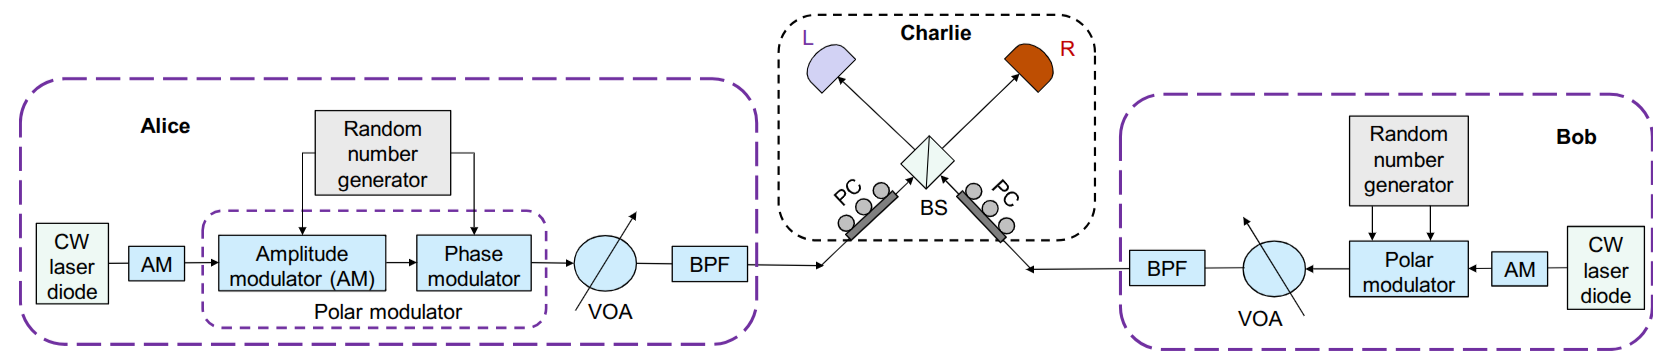
\includegraphics[width=\textwidth]{chapters/figs/fig-6-20}
	\caption{پیکربندی سیستم کاربردی توزیع کلید کوانتومی میدان-دوقلو. \lr{BPF}: فیلتر میان‌گذر نوری؛ \lr{PC}: کنترل‌کننده قطبش.}
	\label{fig:6-20}
\end{figure}

برای پروتکل \lr{BB84} مبتنی بر \lr{TF}، آلیس و باب داده‌های خام را برای کدگذاری فاز تنها در صورتی نگه می‌دارند که $|k_A - k_B| = 0$ یا $M/2$ باشد (زمانی که هر دو از پایه $X$ استفاده کرده‌اند) و سایر نتایج داده‌های خام حذف می‌شوند. برای $|k_A - k_B| = 0$، زمانی که چارلی حالت بل $|\psi^-\rangle$ را آشکار می‌کند، باب بیت کلید خود را وارونه می‌کند. به‌طور مشابه، برای $|k_A - k_B| = M/2$، زمانی که چارلی حالت بل $|\psi^+\rangle$ را آشکار می‌کند، باب بیت کلید خود را وارونه می‌کند. کسر مخفی برای پروتکل \lr{BB84} مبتنی بر \lr{TF} را می‌توان طبق مرجع \cite{104} به‌صورت زیر تخمین زد:
\begin{equation}
	\begin{aligned}
		Q_{ZZ} &= 2p_d(1-p_d)(1-t)^2 + 4(1-p_d)e^{-\mu T_{tot}/2} [1-(1-p_d)e^{-\mu T_{tot}/2}]t(1-t) \\
		&\quad + [2(1-p_d)e^{-\mu T_{tot}} I_0(\mu T_{tot}) - (1-p_d)e^{-\mu T_{tot}}]t^2 \\
		E_{ZZ} &= \frac{2p_d(1-p_d)(1-t)^2 + 2(1-p_d)e^{-\mu T_{tot}} I_0(\mu T_{tot}) - (1-p_d)e^{-\mu T_{tot}} t^2}{Q_{ZZ}}
	\end{aligned}
	\label{eq:6-53}
\end{equation}
که در آن $T_{tot} = T\eta_d$ است، به‌طوری‌که $T$ گذردهی و $\eta_d$ بازدهی آشکارساز\LTRfootnote{Detector efficiency} می‌باشد. پارامتر $p_d$ نشان‌دهنده نرخ جریان تاریک\LTRfootnote{Dark current rate} آشکارساز آستانه‌ای است. بر اساس روابط \eqref{eq:6-34} و \eqref{eq:6-35}، با قرار دادن $\mu = \nu/2$، $\sigma_1 = \omega/2$ و $\sigma_2 = 0$، کران پایین بازده $y_{1ZZ}^{(TF)}$ طبق مرجع \cite{2} به‌صورت زیر به‌دست می‌آید:
\begin{equation}
	y_{1ZZ}^{(TF)} \geq \frac{2\nu}{\nu\omega - \omega^2} \left[ q_{\omega/2}e_{\omega/2} - \frac{\omega^2}{\nu^2} q_{\nu/2}e_{\nu/2} - q_0 \left(1 - \frac{\omega^2}{\nu^2}\right) \right]
	\label{eq:6-54}
\end{equation}
که در آن $q_0 = 2p_d(1-p_d)$ است. با به‌کارگیری روش حالت فریب \cite{37,38,39,40,41,42,43,44,45,46,47,48,49,50,51,52,53,54,55,56,57,58,59,60,61,62,63,64,65,66,67,68,69,103,104}، بازده $y_{1XX}^{(TF)}$ و \lr{QBER} یعنی $e_{XX}^{(b1)}$ به‌صورت زیر محدود می‌شوند:
\begin{equation}
	\begin{aligned}
		y_{1XX}^{(TF)} &\geq \frac{\nu}{\nu\omega - \omega^2} \left[ q_w^{(XX)} e_w - \frac{\omega^2}{\nu^2} q_v^{(XX)} e_v - q_0 \left(1 - \frac{\omega^2}{\nu^2}\right) \right] = y_{1XX}^{(TF,LB)} \\
		e_{XX}^{(b1)} &\geq \frac{q_w^{(XX)} e_w Q_w^{(XX)} - q_0 e_{b0} w}{y_{1XX}^{(TF,LB)}}
	\end{aligned}
	\label{eq:6-55}
\end{equation}
که در آن برای حالت خلاء \lr{TF}، $e_{b0} = 1/2$ است و $Q_w^{(XX)}$ باید به‌صورت تجربی تعیین شود.

به‌عنوان نمونه، در شکل \ref{fig:6-21} مقایسه‌ای بین پروتکل \lr{TF-QKD} تطبیق فاز\LTRfootnote{Phase-matching (PM)} (\lr{PM}) معرفی‌شده در مرجع \cite{101} با پروتکل \lr{MDI-QKD} \cite{83} و پروتکل \lr{BB84} مبتنی بر حالت فریب \cite{37} ارائه شده است. پارامترهای سیستم به‌صورت زیر انتخاب شده‌اند: بازدهی آشکارساز $\eta_d = 0.25$، ناکارآمدی مصالحه\LTRfootnote{Reconciliation inefficiency} $f_e = 1.15$، نرخ شمارش تاریک\LTRfootnote{Dark count rate} $p_d = 8 \times 10^{-8}$، خطای عدم انطباق\LTRfootnote{Misalignment error} $e_d = 1.5\%$ و تعداد قطاع‌های فاز\LTRfootnote{Phase slices} برای \lr{PM TF-QKD} برابر با $M = 16$ تنظیم شده است. در رابطه با محیط ارسال، فرض شده است که از فیبر با تلفات بسیار کم\LTRfootnote{Ultra-low-loss fiber} گزارش‌شده در سال‌های اخیر با تضعیف $0.1419$ \lr{dB/km} (در طول‌موج $1560$ نانومتر) استفاده شده است \cite{105}. در همان شکل، کران \lr{PLOB} روی نرخ کلید خطی نیز ارائه شده است. به‌وضوح، طرح \lr{PM TF-QKD} برای مسافت‌های بیشتر از $162$ کیلومتر، عملکرد بهتری نسبت به پروتکل \lr{BB84} حالت فریب دارد. این طرح در تمام مسافت‌ها نسبت به پروتکل \lr{MDI-QKD} برتری داشته و در مسافت $322$ کیلومتر از کران \lr{PLOB} فراتر می‌رود. در نهایت، پروتکل \lr{PM TF-QKD} می‌تواند حتی به مسافت $623$ کیلومتر نیز دست یابد؛ هرچند متأسفانه مقدار \lr{SKR} نرمالیزه‌شده در این مسافت نسبتاً کم است. برای محاسبات، از روابط ارائه شده در پیوست \lr{B} مرجع \cite{101} با اصلاح چند غلط تایپی آشکار استفاده شده است.


\begin{figure}[ht]
	\centering
	 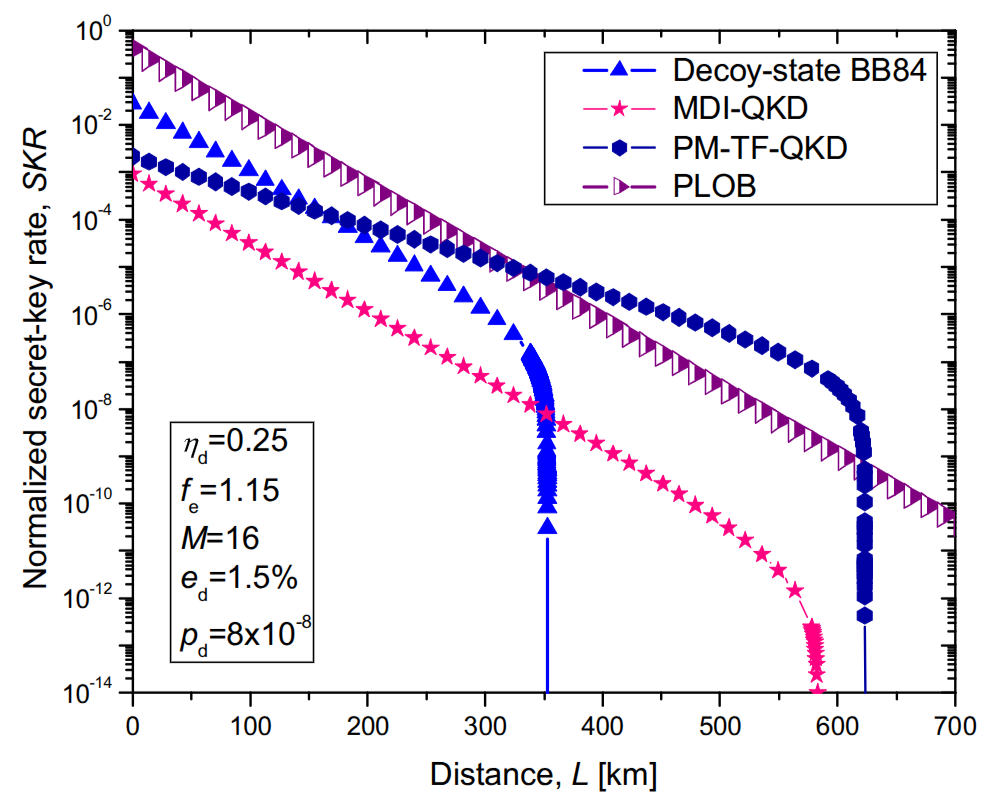
\includegraphics[width=0.5\textwidth]{chapters/figs/fig-6-21}
	\caption{پروتکل توزیع کلید کوانتومی (\lr{QKD}) میدان-دوقلوی آماده‌سازی-و-اندازه‌گیری در مقابل پروتکل‌های \lr{MDI-QKD} و \lr{BB84} حالت فریب در نمودار نرخ کلید مخفی نرمالیزه‌شده برحسب مسافت ارسال.}
	\label{fig:6-21}
\end{figure}

\section{مصالحه اطلاعات و تقویت حریم خصوصی}
\label{sec:6-9}
همان‌طور که پیش‌تر بحث شد، کلید خام ناقص است و ما باید مصالحه اطلاعات و تقویت حریم خصوصی را انجام دهیم تا همبستگی بین دنباله‌های آلیس و باب را افزایش داده و در عین حال، اطلاعات متقابل شنودگر (ایو) درباره نتیجه را تا سطح امنیت مطلوب کاهش دهیم.

\subsection{مصالحه اطلاعات}
\label{sec:6-9-1}
\lr{EA-QKD} شباهت‌های خاصی به پروتکل تولید (توافق) کلید مخفی نوع منبع دارد که در امنیت لایه فیزیکی مطرح است \cite{2}. در این مدل، آلیس، باب و ایو به پورت‌های خروجی متناظر $X$، $Y$ و $Z$ از منبعی که با تابع چگالی احتمال (\lr{PDF}) مشترک $f_{XYZ}$ مشخص می‌شود، دسترسی دارند. هر یک از آن‌ها تحقق‌های مستقل و با توزیع یکسان (\lr{i.i.d.}) از منبع را مشاهده می‌کنند که به‌ترتیب با $X^n$، $Y^n$ و $Z^n$ نشان داده می‌شوند. با توجه به اینکه تحقق‌های آلیس و باب کاملاً همبسته نیستند، آن‌ها باید خطاهای ناشی از اختلافات را اصلاح کنند. این مرحله در تولید کلید مخفی و \lr{QKD} معمولاً به عنوان مصالحه اطلاعات (یا صرفاً مصالحه) شناخته می‌شود. فرآیند مصالحه را می‌توان به عنوان مورد خاصی از کدگذاری منبع با اطلاعات جانبی\LTRfootnote{Source coding with side information} در نظر گرفت \cite{11, 106}. برای کدگذاری منبع $X$، از قضیه کدگذاری منبع شانون\LTRfootnote{Shannon's source coding theorem} می‌دانیم که نرخ $R_x$ باید تا حد امکان کوچک باشد اما نباید از آنتروپی منبع کمتر باشد؛ به عبارت دیگر $R_x > H(X)$. برای کدگذاری مشترک منبع ($XY, f_{XY}$) به نرخ $R > H(X,Y)$ نیاز داریم. اگر منابع را به‌طور مجزا کدگذاری کنیم، نرخ مورد نیاز $R > H(X) + H(Y)$ خواهد بود. با این حال، اسلپیان و ولف\LTRfootnote{Slepian and Wolf} در مرجع \cite{106} نشان داده‌اند که نرخ $R = H(X,Y)$ حتی برای کدگذاری مجزای منابع همبسته نیز کافی است. این ادعا معمولاً به عنوان قضیه اسلپیان-ولف شناخته می‌شود و می‌تواند به‌صورت زیر فرمول‌بندی شود \cite{11, 106}: ناحیه نرخ دستیابی‌پذیر\LTRfootnote{Achievable rate region} $\mathcal{R}$ (که برای آن احتمال خطا به صفر میل می‌کند) برای کدگذاری مجزای منبع همبسته ($XY, f_{XY}$) توسط رابطه زیر داده می‌شود:
\begin{equation}
	\mathcal{R} = \left\{ (R_x, R_y) : R_x \geq H(X|Y), R_y \geq H(Y|X), R_x + R_y \geq H(X,Y) \right\}
	\label{eq:6-56}
\end{equation}
شکل معمول ناحیه اسلپیان-ولف در شکل \ref{fig:6-22} ارائه شده است. اکنون اگر فرض کنیم که $(X, f_X)$ باید در حالی که $(Y, f_Y)$ به عنوان اطلاعات جانبی در دسترس است فشرده شود، آنگاه $H(X|Y)$ برای توصیف $X$ کافی است.







\begin{figure}[ht]
	\centering
	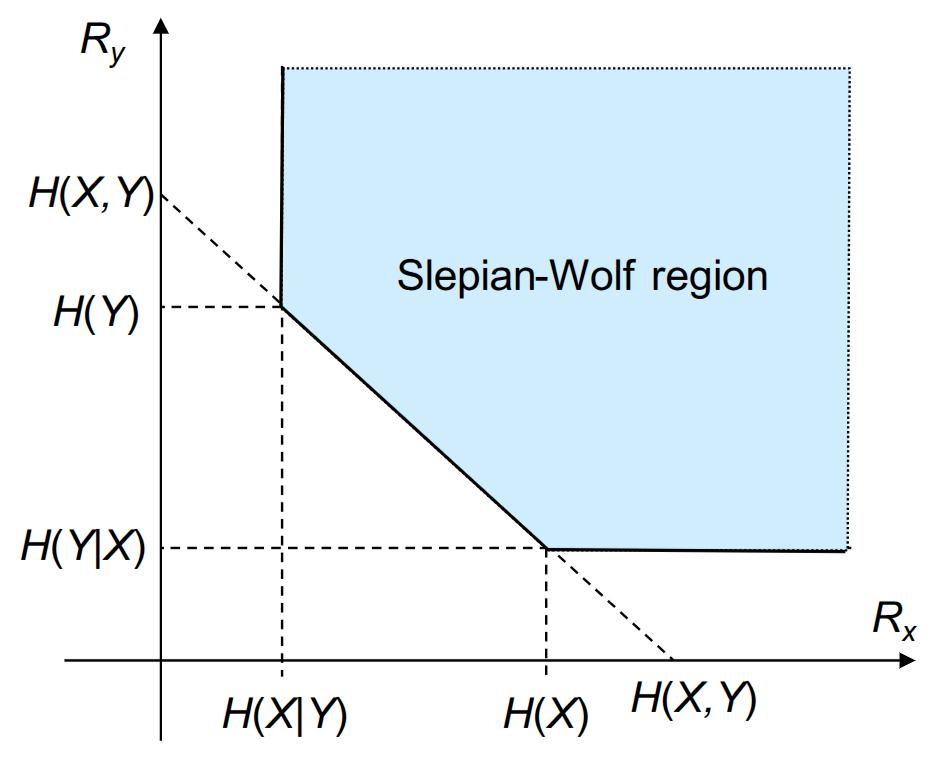
\includegraphics[width=0.5\textwidth]{chapters/figs/fig-6-22}
	\caption{ناحیه نرخ دستیابی‌پذیر معمول اسلپیان-ولف برای یک منبع همبسته ($XY, f_{XY}$).}
	\label{fig:6-22}
\end{figure}

با بازگشت به مسئله مصالحه خود، آلیس مشاهدات خود $X^n$ را فشرده می‌کند و باب آن‌ها را با کمک اطلاعات جانبی همبسته $Y^n$ رمزگشایی می‌نماید که در شکل \ref{fig:6-23} نشان داده شده است. رمزگذار منبع را می‌توان از کد کانال دستیابی‌پذیر به ظرفیت استخراج کرد. برای یک کد بررسی توازن کم‌چگال (\lr{LDPC})\LTRfootnote{Low-density parity-check (LDPC)} با مشخصات $(n,k)$، می‌توان از یک ماتریس بررسی توازن $\bm{H}$ با ابعاد $(n-k) \times n$ برای تولید سندرم\LTRfootnote{Syndrome} به‌صورت $\bm{s} = \bm{H}\bm{x}$ استفاده کرد که در آن $\bm{x}$ بردار مشاهده منبع گسسته بدون حافظه\LTRfootnote{Discrete Memoryless Source (DMS)} آلیس به طول $n$ است. از آنجا که $\bm{x}$ یک کلمه کد\LTRfootnote{Codeword} نیست، بردار سندرم با بردار تمام‌صفر متفاوت خواهد بود. بردار سندرم دارای طول $n-k$ است و می‌توان آن را به‌صورت $\bm{s} = [s_1, s_2, \dots, s_{n-k}]^T$ نمایش داد. به‌وضوح، بردار سندرم از طریق کانال عمومی احرازهویت‌شده (بدون خطا) به سمت باب ارسال می‌شود.

\begin{figure}[ht]
	\centering
	 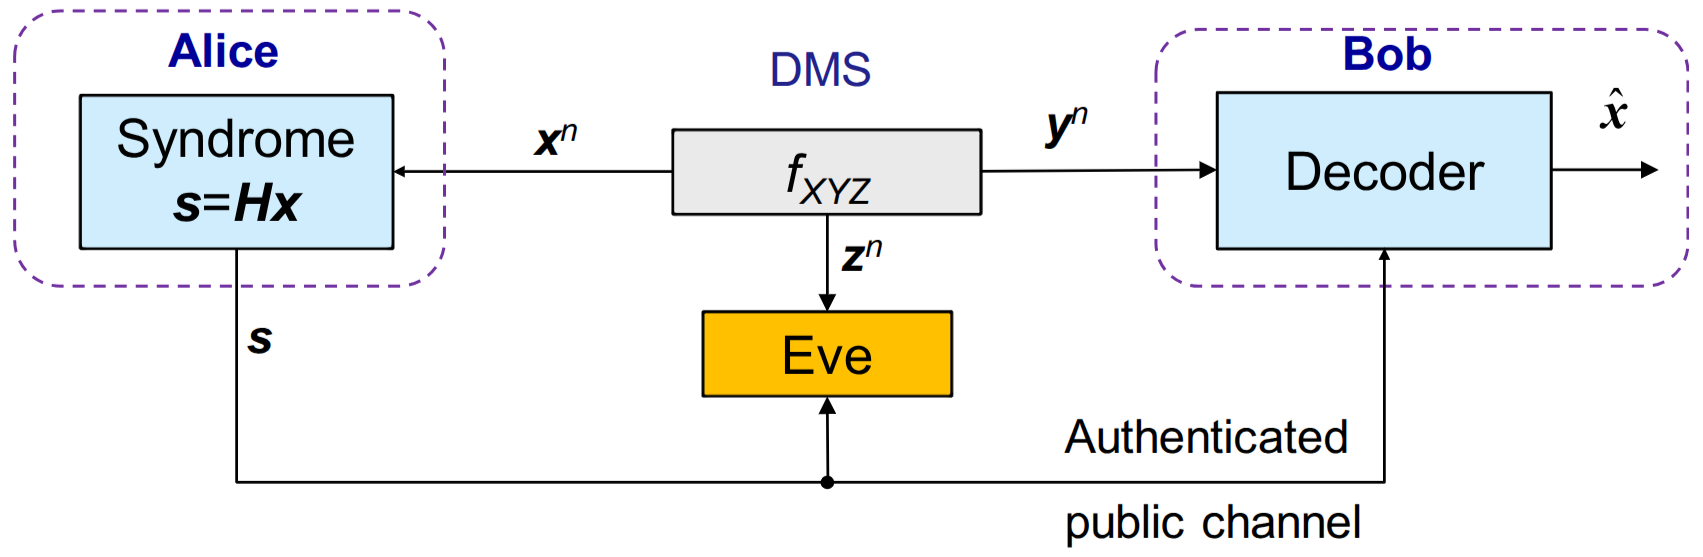
\includegraphics[width=0.8\textwidth]{chapters/figs/fig-6-23}
	\caption{مسئله مصالحه که به‌صورت کدگذاری منبع با اطلاعات جانبی مبتنی بر سندرم نمایش داده شده است.}
	\label{fig:6-23}
\end{figure}

هنگامی که باب بردار سندرم $\bm{s}$ را دریافت می‌کند، رمزگشای او سعی می‌کند بردار $\bm{x}$ را بر اساس $\bm{s}$ و بردار مشاهده باب $\bm{y}$ تعیین کند، به‌طوری که احتمال پسین\LTRfootnote{Posterior probability} را بیشینه نماید:
\begin{equation}
	\hat{\bm{x}} = \max P(\bm{y}|\bm{x}, \bm{s})
	\label{eq:6-57}
\end{equation}
و به‌وضوح، مسئله رمزگشایی مشابه رمزگشایی با بیشینه احتمال پسین (\lr{MAP})\LTRfootnote{Maximum a posteriori probability (MAP)} است. نرخ فشرده‌سازی برابر با $(n-k)/n = 1 - k/n$ است، در حالی که نرخ کد خطی $k/n$ می‌باشد. تعداد بیت‌های سندرم مورد نیاز برابر است با:
\begin{equation}
	n - k \geq nH(X^n|Y^n) = nH(X|Y)
	\label{eq:6-58}
\end{equation}
در عمل، الگوریتم‌های مصالحه کاربردی، یک مقدار بالاسری\LTRfootnote{Overhead} $OH > 0$ معرفی می‌کنند، به‌طوری که تعداد بیت‌های ارسال شده در کانال عمومی برابر با $nH(X|Y)(1 + OH)$ است. در پایان مرحله مصالحه، آلیس و باب دنباله مشترک $X^n$ با آنتروپی $nH(X)$ را با احتمال بالا به اشتراک می‌گذارند، بنابراین بازدهی مصالحه $\beta$ را می‌توان به‌صورت زیر نوشت:
\begin{equation}
	\beta = \frac{nH(X) - nH(X|Y)(1 + OH)}{nI(X; Y)} = 1 - OH \frac{H(X|Y)}{I(X; Y)} \leq 1
	\label{eq:6-59}
\end{equation}

پیچیدگی رمزگشایی \lr{MAP} در هنگام استفاده از کدگذاری \lr{LDPC} به‌طور بازدارنده‌ای بالا است؛ در عوض باید از الگوریتم مجموع-حاصل‌ضرب (\lr{SPA})\LTRfootnote{Sum-product algorithm (SPA)} با پیچیدگی کم (که با نام الگوریتم انتشار باور\LTRfootnote{Belief-propagation algorithm} نیز شناخته می‌شود) مطابق آنچه در مرجع \cite{107} توصیف شده است، استفاده کرد. با توجه به اینکه مشاهده آلیس $\bm{x}$ یک کلمه کد نیست، بیت‌های سندرم غیرصفر هستند. برای در نظر گرفتن این مسئله، هنگامی که بیت سندرم متناظر $s_c$ برابر با $1$ است، باید علامت نسبت لگاریتمی درست‌نمایی (\lr{LLR})\LTRfootnote{Log-likelihood ratio (LLR)} ارسالی از گره بررسی\LTRfootnote{Check node} $c$-ام به گره متغیر\LTRfootnote{Variable node} $v$-ام را تغییر دهیم. بر اساس مرجع \cite{108}، می‌توانیم \lr{SPA} در حوزه لگاریتم را به‌صورت زیر خلاصه کنیم. برای بهبود وضوح ارائه، از شاخص $v = 1, \dots, n$ برای نشان دادن گره‌های متغیر و از شاخص $c = 1, \dots, n-k$ برای نشان دادن گره‌های بررسی استفاده می‌کنیم. علاوه بر این، از نمادگذاری‌های زیر استفاده می‌شود: (الف) $N(c)$ برای نشان دادن {مجموعه گره‌های $v$ متصل به گره $c$}، (ب) $N(c) \setminus \{v\}$ برای نشان دادن {مجموعه گره‌های $v$ متصل به گره $c$ به‌جز گره $v$}، (ج) $N(v)$ برای نشان دادن {مجموعه گره‌های $c$ متصل به گره $v$}، و (د) $N(v) \setminus \{c\}$ برای نشان دادن {مجموعه گره‌های $c$ متصل به گره $v$ به‌جز گره $c$}.

فرمول‌بندی \lr{SPA} در حوزه لگاریتم برای کدگذاری منبع با اطلاعات جانبی به‌صورت زیر ارائه می‌شود:

\begin{enumerate}
	\item \textbf{مقداردهی اولیه:} برای گره‌های متغیر $v = 1, 2, \dots, n$؛ پیام‌های بیرونی\LTRfootnote{Extrinsic messages} $L_{vc}$ ارسالی از گره متغیر (\lr{v-node}) $v$ به گره بررسی (\lr{c-node}) $c$ را با نسبت‌های لگاریتمی درست‌نمایی کانال که با $L_{ch}(v)$ نشان داده می‌شوند، مقداردهی اولیه کنید؛ یعنی $L_{vc} = L_{ch}(v)$.
	\item \textbf{قانون به‌روزرسانی گره بررسی (گره $c$):} برای گره‌های بررسی $c = 1, 2, \dots, n-k$؛ مقدار $L_{cv} = (1 - 2s_c) \sum_{N(c) \setminus \{v\}} L_{v'c}$ را محاسبه کنید. عملگر باکس-پلاس\LTRfootnote{Box-plus operator} به‌صورت زیر تعریف می‌شود:
	\begin{equation}
		L_1 + L_2 = \prod_{k=1}^2 \text{sign}(L_k) \cdot \phi \left( \sum_{k=1}^2 \phi(|L_k|) \right)
		\label{eq:6-60}
	\end{equation}
	که در آن $\phi(x) = -\log \tanh(x/2)$ است. عملگر باکس برای مولفه‌های $|N(c) \setminus \{v\}|$ با اعمال بازگشتی نسخه دو-مولفه‌ای تعریف شده در بالا به‌دست می‌آید.
	\item \textbf{قانون به‌روزرسانی گره متغیر (گره $v$):} برای $v = 1, 2, \dots, n$؛ مقدار $L_{vc} = L_{ch}(v) + \sum_{N(v) \setminus \{c\}} L_{c'v}$ را برای تمام گره‌های $c$ که عنصر سطر $c$-ام و ستون $v$-ام ماتریس بررسی توازن $\bm{H}$ آن‌ها یک است (یعنی $h_{cv} = 1$)، تنظیم کنید.
	\item \textbf{تصمیم‌گیری بیت‌ها:} مقدار $L(v)$ را برای $v = 1, \dots, n$ با رابطه $L(v) = L_{ch}(v) + \sum_{N(v)} L_{c'v}$ به‌روزرسانی کرده و تصمیم‌گیری‌ها را به‌صورت زیر انجام دهید:
	$\hat{x}_v = 1$ اگر $L(v) < 0$ (در غیر این صورت $\hat{x}_v = 0$).
\end{enumerate}

بنابراین تنها تفاوت نسبت به \lr{SPA} متعارف در حوزه لگاریتم، معرفی ضریب ضرب $(1 - 2s_c)$ در قانون به‌روزرسانی گره $c$ است. علاوه بر این، درست‌نمایی‌های کانال $L_{ch}(v)$ باید از توزیع مشترک $f_{XY}$ به‌صورت $L_{ch}(v) = \log [f_{XY}(x_v = 0|y_v) / f_{XY}(x_v = 1|y_v)]$ محاسبه شوند. از آنجا که قانون به‌روزرسانی گره $c$ شامل توابع $\log$ و $\tanh$ است، می‌تواند از نظر محاسباتی سنگین باشد و برای کاهش پیچیدگی، باید از تقریب‌های با پیچیدگی کاهش‌یافته استفاده کرد.


تحلیل تقویت حریم خصوصی بر پایه آنتروپی شانون نیست، بلکه بر اساس آنتروپی رنی\LTRfootnote{Rényi entropy} انجام می‌شود \cite{114, 115, 116}. برای متغیر تصادفی گسسته $\bm{X}$ که مقادیری را از فضای نمونه\LTRfootnote{Sample space} $\{x_1, \dots, x_n\}$ می‌گیرد و طبق توزیع $P_{\bm{X}} = \{p_1, \dots, p_n\}$ توزیع شده است، آنتروپی رنی از مرتبه $\alpha$ برای $\bm{X}$ طبق مرجع \cite{115} به‌صورت زیر تعریف می‌شود:
\begin{equation}
	R_\alpha(\bm{X}) = \frac{1}{1-\alpha} \log_2 \left( \sum_{x \in \mathcal{X}} [P_{\bm{X}}(x)]^\alpha \right)
	\label{eq:6-60}
\end{equation}

آنتروپی رنی از مرتبه دو با نام آنتروپی برخورد\LTRfootnote{Collision entropy} نیز شناخته می‌شود. از نامساوی ینسن\LTRfootnote{Jensen's inequality} \cite{11} نتیجه می‌گیریم که آنتروپی برخورد توسط آنتروپی شانون محدود می‌شود، یعنی $R_2(\bm{X}) \leq H(\bm{X})$. در حالتی که $\alpha \to \infty$، آنتروپی رنی به کمینه-آنتروپی\LTRfootnote{Min-entropy} تبدیل می‌شود:
\begin{equation}
	\lim_{\alpha \to \infty} R_\alpha(\bm{X}) = -\log_2 \max_{x \in \mathcal{X}} P_{\bm{X}}(x) = H_\infty(\bm{X})
	\label{eq:6-61}
\end{equation}
در نهایت، با اعمال قاعده هوپیتال\LTRfootnote{l'Hôpital's rule} در حالت $\alpha \to 1$، آنتروپی رنی به همان آنتروپی شانون تبدیل می‌گردد:
\begin{equation}
	\lim_{\alpha \to 1} R_\alpha(\bm{X}) = -\sum_x P_{\bm{X}}(x) \log_2 P_{\bm{X}}(x) = H(\bm{X})
	\label{eq:6-62}
\end{equation}
ویژگی‌های آنتروپی رنی در مرجع \cite{115} خلاصه شده است. در رابطه با آنتروپی رنی شرطی، سه تعریف مختلف در مرجع \cite{116} به‌تفصیل مورد بحث قرار گرفته است که ما اولین مورد از آن‌ها را برمی‌گزینیم. فرض کنید توزیع مشترک برای $(\bm{X}, \bm{Y})$ با $P_{\bm{X,Y}}$ و توزیع برای $\bm{X}$ با $P_{\bm{X}}$ نشان داده شود. علاوه بر این، فرض کنید آنتروپی رنی متغیرهای تصادفی شرطی $\bm{X}|\bm{Y}=y$ که طبق $P_{\bm{X}|\bm{Y}=y}$ توزیع شده‌اند، با $R_\alpha(\bm{X}|\bm{Y}=y)$ نشان داده شود. آنگاه آنتروپی رنی شرطی را می‌توان به‌صورت زیر تعریف کرد:
\begin{equation}
	R_\alpha(\bm{X}|\bm{Y}) = \sum_y P_{\bm{Y}}(y) R_\alpha(\bm{X}|\bm{Y}=y) = \frac{1}{1-\alpha} \sum_y P_{\bm{Y}}(y) \log_2 \sum_x P_{\bm{X}|\bm{Y}}(x|y)^\alpha
	\label{eq:6-63}
\end{equation}
اطلاعات رنی متقابل\LTRfootnote{Mutual Rényi information} را نیز می‌توان به‌صورت زیر تعریف کرد:
\begin{equation}
	I_\alpha(\bm{X}; \bm{Y}) = R_\alpha(\bm{X}) - R_\alpha(\bm{X}|\bm{Y})
	\label{eq:6-64}
\end{equation}
که نسبت به $R_\alpha(\bm{Y}) - R_\alpha(\bm{Y}|\bm{X})$ متقارن نیست. علاوه بر این، همان‌طور که در مراجع \cite{115, 116} بحث شده است، این مقدار حتی می‌تواند منفی باشد.

بنت و همکاران در مرجع \cite{23} قضیه تقویت حریم خصوصی زیر را اثبات کرده‌اند (قضیه ۳ را ببینید): فرض کنید $\bm{X}$ یک متغیر تصادفی با توزیع $P_{\bm{X}}$ و آنتروپی رنی مرتبه دو $R_2(\bm{X})$ باشد. همچنین فرض کنید $\bm{G}$ متغیر تصادفی نشان‌دهنده انتخاب تصادفی و یکنواخت عضوی از توابع هش سراسری $\{0,1\}^n \to \{0,1\}^k$ باشد. در این صورت نامساوی‌های زیر برقرار هستند \cite{23}:
\begin{equation}
	H(\bm{G}(\bm{X})|\bm{G}) \leq R_2(\bm{G}(\bm{X})|\bm{G}) \leq k + \log_2 (1 + 2^{k-R_2(\bm{X})}) \leq k + \frac{2^{k-R_2(\bm{X})}}{\ln 2}
	\label{eq:6-65}
\end{equation}
بنت و همکاران همچنین نتیجه\LTRfootnote{Corollary} زیر را از قضیه تقویت حریم خصوصی اثبات کرده‌اند \cite{23} (همچنین ببینید \cite{110}): فرض کنید $\bm{S} \in \{0,1\}^n$ متغیر تصادفی نشان‌دهنده دنباله مشترک بین آلیس و باب باشد و $\bm{E}$ متغیر تصادفی نشان‌دهنده دانشی باشد که ایو توانسته درباره $\bm{S}$ به‌دست آورد، به‌طوری‌که یک تحقق خاص از $\bm{E}$ با $e$ نشان داده می‌شود. اگر معلوم باشد که آنتروپی رنی شرطی مرتبه دو $R_2(\bm{S}|\bm{E}=e)$ حداقل برابر با $r_2$ است و آلیس و باب کلید مخفی را به‌صورت $\bm{K} = \bm{G}(\bm{S})$ انتخاب کنند (که در آن $\bm{G}$ یک تابع هش است که به‌طور تصادفی و یکنواخت از خانواده توابع هش جهانی-$2$ در $\{0,1\}^n \to \{0,1\}^k$ انتخاب شده است)، آنگاه رابطه زیر معتبر است:
\begin{equation}
	H(\bm{K}|\bm{G}, \bm{E}=e) \geq k - \frac{2^{k-r_2}}{\ln 2}
	\label{eq:6-66}
\end{equation}

کاچین\LTRfootnote{Cachin} در مرجع \cite{117} لم آنتروپی رنی زیر را اثبات کرده است (همچنین ببینید \cite{118}): فرض کنید $\bm{X}$ و $\bm{Q}$ دو متغیر تصادفی باشند و $s > 0$. آنگاه با احتمالی حداقل برابر با $1 - 2^{-s}$، رابطه زیر برقرار است \cite{117, 118}:
\begin{equation}
	R_2(\bm{X}) \geq R_2(\bm{X}|\bm{Q}=q) - \log |\bm{Q}| - 2s - 2
	\label{eq:6-67}
\end{equation}
اطلاعات کل در دسترس ایو متشکل از مشاهدات او $\bm{Z}^n$ از منبع تصادفی مشترک و بیت‌های اضافی مبادله شده در مرحله مصالحه اطلاعات روی کانال عمومی احرازهویت‌شده است که با متغیر تصادفی $\bm{Q}$ نشان داده می‌شود. بر اساس لم کاچین، می‌توانیم بنویسیم:
\begin{equation}
	R_2(\bm{S}|\bm{Z}^n=z_n) \geq R_2(\bm{S}|\bm{Z}^n=z_n, \bm{Q}=q) - \log |\bm{Q}| - 2s - 2 \text{ با احتمال } 1 - 2^{-s}
	\label{eq:6-68}
\end{equation}
می‌دانیم که $R_2(\bm{X}) \leq H(\bm{X})$، بنابراین نتیجه می‌گیریم که $R_2(\bm{S}|\bm{Z}^n=z_n) \leq H(\bm{S}|\bm{Z}^n=z_n)$ و از این رو، می‌توانیم $R_2(\bm{S}|\bm{Z}^n=z_n)$ را به‌صورت زیر از بالا محدود کنیم:
\begin{equation}
	R_2(\bm{S}|\bm{Z}^n=z_n) \leq nH(X|Z)
	\label{eq:6-69}
\end{equation}
بر اساس رابطه \eqref{eq:6-68}، می‌توانیم $R_2(\bm{S}|\bm{Z}^n=z_n, \bm{Q}=q)$ را به‌صورت زیر از پایین محدود کنیم:
\begin{equation}
	R_2(\bm{S}|\bm{Z}^n=z_n, \bm{Q}=q) \geq nH(X|Z) - \log |\bm{Q}| - 2s - 2 \text{ با احتمال } 1 - 2^{-s}
	\label{eq:6-70}
\end{equation}
از آنجا که تعداد بیت‌های مبادله شده در کانال عمومی، $\log |\bm{Q}|$، تقریباً برابر با $nH(X|Y)(1 + OH)$ است، برای $n$ به اندازه کافی بزرگ، نامساوی قبلی به‌صورت زیر در می‌آید:
\begin{equation}
	\underbrace{nH(X|Z) - nH(X|Y)(1 + OH) - 2s - 2}_{r_2} \geq R_2(\bm{S}|\bm{Z}^n=z_n, \bm{Q}=q) \text{ با احتمال } 1 - 2^{-s}
	\label{eq:6-71}
\end{equation}
از رابطه \eqref{eq:6-66} نتیجه می‌گیریم که $k - r_2 = -k_2 < 0$ است، که تضمین می‌کند برای $k_2 > 0$، عدم قطعیت ایو درباره کلید با احتمالی حداقل برابر با $1 - 2^{-s}$ به‌صورت زیر از پایین محدود می‌شود:
\begin{equation}
	H(\bm{K}|\bm{E}) \geq k - \frac{2^{-k_2}}{\ln 2}
	\label{eq:6-72}
\end{equation}


\section{توزیع کلید کوانتومی با متغیر پیوسته}
\label{sec:6-10}
خوانندگانی که با اپتیک کوانتومی آشنا نیستند، باید ابتدا بخش‌های \ref{sec:5-4} و \ref{sec:5-8} در فصل \ref{chap:5} را مطالعه کنند. \lr{CV-QKD} را می‌توان یا با استفاده از آشکارسازی هموداین\LTRfootnote{Homodyne detection} پیاده‌سازی کرد که در آن در هر لحظه تنها یک مؤلفه مربعی\LTRfootnote{Quadrature component} اندازه‌گیری می‌شود (به دلیل اصل عدم قطعیت)، همان‌طور که در شکل \ref{fig:6-24} نشان داده شده است؛ و یا با استفاده از آشکارسازی هتروداین\LTRfootnote{Heterodyne detection (HD)} (\lr{HD}) که در آن از یک \lr{BS} و دو فتودتکتور متعادل\LTRfootnote{Balanced photodetectors} برای اندازه‌گیری هم‌زمان هر دو مؤلفه مربعی استفاده می‌شود، مطابق آنچه در شکل \ref{fig:6-25} تصویر شده است. \lr{HD} می‌تواند اطلاعات متقابل بین آلیس و باب را در مقایسه با طرح آشکارسازی هموداین دوبرابر کند، که البته این امر به قیمت تلفات اضافی $3$ \lr{dB} ناشی از \lr{BS} تمام می‌شود. برای کاهش نویز فاز، سیگنال‌های کوانتومی معمولاً همراه با یک تُن پایلوت\LTRfootnote{Pilot-tone} پرتوانِ تسهیم‌شده در حوزه زمان ارسال می‌شوند تا پایه‌های اندازه‌گیری آلیس و باب با یکدیگر هم‌راستا شوند. با قضاوت از روی تعداد فزاینده مقالات مرتبط با \lr{CV-QKD} \cite{8, 119, 120, 121, 122, 123, 124, 125, 126, 127, 128, 129, 130, 131, 132, 133, 134, 135, 136, 137, 138, 139, 140, 141, 142, 143, 144, 145}، پژوهش‌ها در این حوزه به دلیل سازگاری آن‌ها با فناوری‌های پیشرفته مخابرات نوری در حال شتاب گرفتن است. سیستم \lr{CV-QKD} هنگام استفاده از مصالحه مستقیم\LTRfootnote{Direct reconciliation}، با محدودیت تلفات $3$ \lr{dB} در گذردهی مواجه می‌شود. برای جلوگیری از این مشکل، از روش‌های مصالحه معکوس\LTRfootnote{Reverse reconciliation} \cite{146} یا پس‌گزینش\LTRfootnote{Postselection} \cite{127} استفاده می‌شود. استراتژی‌های مختلف شنود که پیش‌تر بحث شد، برای سیستم‌های \lr{CV-QKD} نیز قابل اعمال هستند. نشان داده شده است که برای مدولاسیون گاوسی، حمله گاوسی بهینه ترین حمله برای هر دو نوع حملات انفرادی \cite{133} و حملات دسته‌جمعی \cite{134, 135} است. در این بخش از فصل، تمرکز خود را بر \lr{CV-QKD} با مدولاسیون گاوسی معطوف می‌کنیم. برای پیاده‌سازی \lr{CV-QKD}، هم می‌توان از حالت‌های فشرده\LTRfootnote{Squeezed states} و هم از حالت‌های همدوس استفاده کرد.

\begin{figure}[ht]
	\centering
	 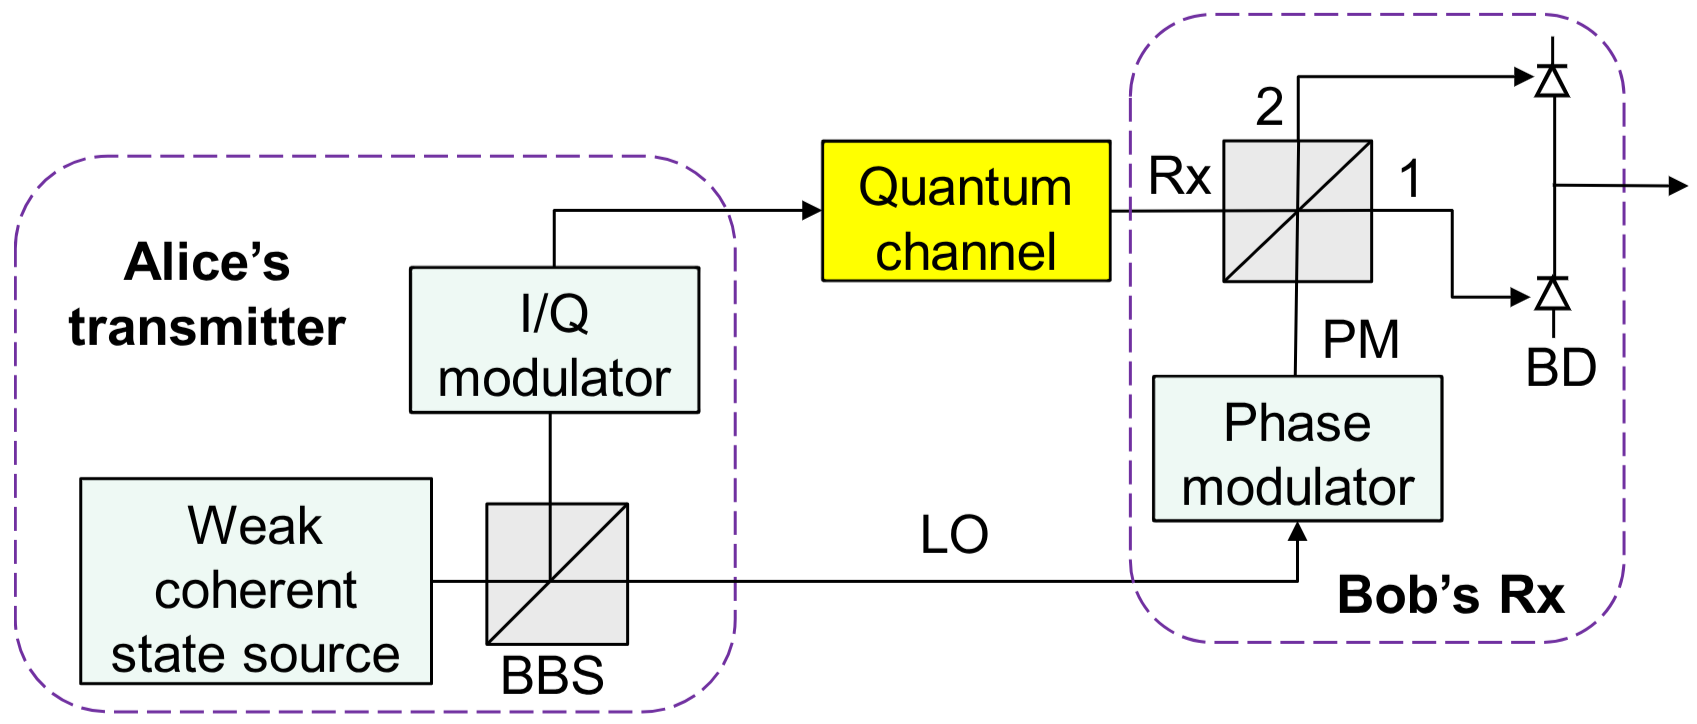
\includegraphics[width=0.8\textwidth]{chapters/figs/fig-6-24}
	\caption{پروتکل‌های توزیع کلید کوانتومی با متغیر پیوسته مبتنی بر مدولاسیون گاوسی با آشکارسازی هموداین. \lr{BBS}: تقسیم‌کننده پرتو متعادل؛ \lr{BD}: آشکارساز متعادل.}
	\label{fig:6-24}
\end{figure}

\begin{figure}[ht]
	\centering
	 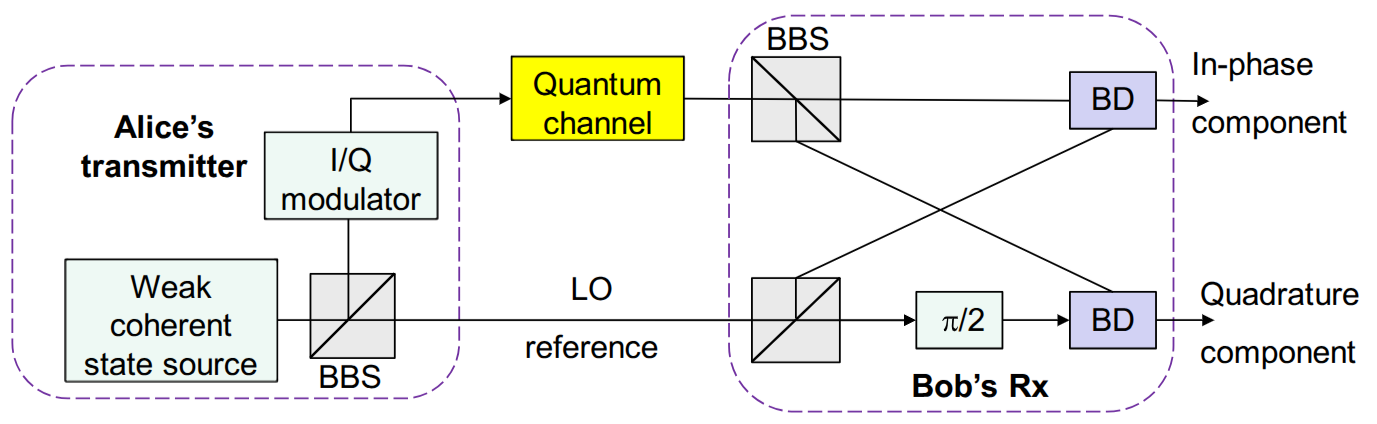
\includegraphics[width=0.8\textwidth]{chapters/figs/fig-6-25}
	\caption{پروتکل‌های توزیع کلید کوانتومی با متغیر پیوسته مبتنی بر مدولاسیون گاوسی با آشکارسازی هتروداین. \lr{BBS}: تقسیم‌کننده پرتو متعادل؛ \lr{BD}: آشکارساز متعادل (نشان داده شده در شکل \ref{fig:6-24}).}
	\label{fig:6-25}
\end{figure}



\subsection{طرح‌های آشکارسازی هموداین و هتروداین}
\label{subsec:6-10-1}
در طرح آشکارسازی هموداین\LTRfootnote{Homodyne detection} که در شکل \ref{fig:6-24} ارائه شده و رایج‌ترین نوع اندازه‌گیری در سیستم‌های متغیر پیوسته (\lr{CV}) محسوم می‌شود، ما یکی از دو مؤلفه مربعی را اندازه‌گیری می‌کنیم؛ زیرا طبق اصل عدم قطعیت، نمی‌توانیم هر دو مؤلفه مربعی را به‌طور هم‌زمان اندازه‌گیری کنیم. عملگرهای اندازه‌گیری، تصویرگرهایی روی پایه مؤلفه مربعی $|I\rangle\langle I|$ یا $|Q\rangle\langle Q|$ هستند و نتایج متناظر دارای تابع چگالی احتمال (\lr{PDF}) $f(I)$ یا $f(Q)$ می‌باشند که از طریق انتگرال‌گیری حاشیه‌ای\LTRfootnote{Marginal integration} از تابع ویگنر\LTRfootnote{Wigner function} (معرفی شده در رابطه $5.144$) به‌دست می‌آیند، که برای تک‌مُد به‌صورت زیر در می‌آید:
\begin{equation*}
	f(I) = \int W(I, Q) dQ; \quad f(Q) = \int W(I, Q) dI
\end{equation*}
زمانی که بیش از یک مُد بوزونی\LTRfootnote{Bosonic modes} در باریکه نوری وجود داشته باشد، باید هموداین کردن جزئی\LTRfootnote{Partial homodyning} را اعمال کرده و همچنین روی هر دو مؤلفه مربعی تمام مدهای دیگر انتگرال‌گیری انجام دهیم.

در \lr{CV-QKD} مبتنی بر مدولاسیون گاوسی با آشکارسازی هموداین \cite{2, 8} که در شکل \ref{fig:6-24} نشان داده شده است، در هر لحظه تنها یک مؤلفه مربعی اندازه‌گیری می‌شود. این پروتکل معمولاً با نام پروتکل \lr{CV-QKD} \lr{GG02} شناخته می‌شود که به نام نویسندگان آن، گروس‌هانز\LTRfootnote{Grosshans} و گرنژیه\LTRfootnote{Grangier} که آن را در سال $2002$ پیشنهاد کردند، نام‌گذاری شده است \cite{146}. آلیس باریکه لیزر را که به‌عنوان یک منبع \lr{WCS} عمل می‌کند، به‌قدر کافی تضعیف کرده و از تقسیم‌کننده پرتو متعادل (\lr{BBS})\LTRfootnote{Balanced beam splitter (BBS)} برای تقسیم سیگنال به دو بخش استفاده می‌کند. خروجی بالایی \lr{BBS} به‌عنوان ورودی به مدولاتور \lr{I/Q} استفاده می‌شود تا حالت گاوسی را در مکان مورد نظر در صفحه \lr{I-Q} قرار دهد و $|\alpha\rangle = |I + jQ\rangle$ را به‌دست آورد و همچنین واریانس آلیس را کنترل کند. خروجی دوم \lr{BBS} برای ارسال سیگنال مرجع نوسان‌ساز محلی (\lr{LO})\LTRfootnote{Local oscillator (LO)} برای باب استفاده می‌شود. از آنجا که عملکرد تقسیم‌کننده پرتو با ماتریس $B_{BS} = \frac{1}{\sqrt{2}} \begin{bmatrix} 1 & 1 \\ 1 & -1 \end{bmatrix}$ توصیف می‌شود، عملگرهای نابودی\LTRfootnote{Annihilation operators} در خروجی \lr{BBS} باب به‌صورت زیر خواهند بود:
\begin{equation}
	\begin{bmatrix} a_1 \\ a_2 \end{bmatrix} = \frac{1}{\sqrt{2}} \begin{bmatrix} 1 & 1 \\ 1 & -1 \end{bmatrix} \begin{bmatrix} a_{Rx} \\ a_{PM} \end{bmatrix} = \frac{1}{\sqrt{2}} \begin{bmatrix} a_{Rx} + a_{PM} \\ a_{Rx} - a_{PM} \end{bmatrix}
	\label{eq:6-73}
\end{equation}
که در آن عملگرهای تولید (نابودی) در ورودی‌های \lr{BBS} گیرنده ($Rx$ و $PM$) به‌ترتیب با $a_{Rx}^\dagger (a_{Rx})$ و $a_{PM}^\dagger (a_{PM})$ نشان داده شده‌اند. عملگرهای تعداد\LTRfootnote{Number operators} در خروجی‌های یک و دو \lr{BBS} گیرنده اکنون می‌توانند به‌صورت زیر بیان شوند:
\begin{equation}
	\hat{n}_1 = a_1^\dagger a_1 = \frac{1}{2} (a_{PM}^\dagger + a_{Rx}^\dagger)(a_{PM} + a_{Rx}); \quad \hat{n}_2 = a_2^\dagger a_2 = \frac{1}{2} (a_{PM}^\dagger - a_{Rx}^\dagger)(a_{PM} - a_{Rx})
	\label{eq:6-74}
\end{equation}
خروجی یک آشکارساز متعادل (\lr{BD})\LTRfootnote{Balanced detector (BD)} با فرض پاسخ‌دهی فتودیود $R_{ph} = 1 A/W$، (برحسب واحد نویز شات\LTRfootnote{Shot-noise unit} یا \lr{SNU}) به‌صورت زیر داده می‌شود:
\begin{equation}
	\hat{i}_{BD} = 4(\hat{n}_1 - \hat{n}_2) = 4(a_{PM}^\dagger a_{Rx} + a_{Rx}^\dagger a_{PM})
	\label{eq:6-75}
\end{equation}
خروجی مدولاسیون فاز را می‌توان برحسب \lr{SNU} به‌صورت $a_{PM} = |\alpha| e^{j\theta} / \sqrt{2}$ نمایش داد و پس از جایگذاری در \eqref{eq:6-75} به‌دست می‌آوریم:
\begin{equation}
	\hat{i}_{BD} = 4 \left( \frac{|\alpha| e^{-j\theta}}{\sqrt{2}} a_{Rx} + a_{Rx}^\dagger \frac{|\alpha| e^{j\theta}}{\sqrt{2}} \right) = 2\sqrt{2} |\alpha| (e^{-j\theta} a_{Rx} + e^{j\theta} a_{Rx}^\dagger)
	\label{eq:6-76}
\end{equation}
در غیاب ایو، منظومه سیگنال دریافتی $a_{Rx} = (\bm{I} + j\bm{Q})/2$ خواهد بود که پس از جایگذاری در معادله قبلی، به‌دست می‌آوریم:
\begin{equation}
	\begin{aligned}
		\hat{i}_{BD} &= |\alpha| [ (\cos \theta, \sin \theta) \ones \cdot (I \hat{I}, -Q \hat{Q}) + (\cos \theta, \sin \theta) \ones \cdot (I \hat{I}, Q \hat{Q}) ] \\
		&= |\alpha| (\cos \theta \cdot I \hat{I} + \sin \theta \cdot Q \hat{Q}).
		\label{eq:6-77}
	\end{aligned}
\end{equation}
باب مؤلفه هم‌فاز را با انتخاب $\theta = 0$ برای به‌دست آوردن $|\alpha|\bm{I}$ و مؤلفه مربعی را با تنظیم $\theta = \pi/2$ برای به‌دست آوردن $|\alpha|\bm{Q}$ اندازه‌گیری می‌کند.

نظریه آشکارسازی هتروداین\LTRfootnote{Heterodyne detection (HD)} نوری در مرجع \cite{147} توسعه یافته است. \lr{HD} متناظر با تصویر کردن بر روی حالت‌های همدوس است، یعنی $M(\alpha) \sim |\alpha\rangle\langle\alpha|$. این نظریه به \lr{POVM}\LTRfootnote{Positive operator-valued measure} مبتنی بر تصویر کردن روی حالت‌های گاوسی خالص تعمیم یافته است \cite{148, 149}. برای \lr{CV-QKD} با مدولاسیون گاوسی مبتنی بر \lr{HD}، سمت فرستنده مشابه نسخه آشکارسازی همدوس است. در گیرنده \lr{HD} نشان داده شده در شکل \ref{fig:6-25}، سیگنال کوانتومی با استفاده از \lr{BBS} تقسیم می‌شود؛ یک خروجی برای اندازه‌گیری مؤلفه هم‌فاز (شاخه بالایی) استفاده می‌شود، در حالی که خروجی دیگر (شاخه پایینی) به‌عنوان ورودی به \lr{BD} دوم برای آشکارسازی مؤلفه مربعی به کار می‌رود. سیگنال مرجع کلاسیک \lr{LO} نیز توسط \lr{BBS} تقسیم می‌شود، به‌طوری که خروجی بالایی به‌عنوان ورودی به \lr{BD} هم‌فاز استفاده شده و خروجی دیگر، پس از مدولاسیون فاز برای اعمال جابه‌جایی فاز $\pi/2$، به‌عنوان ورودی \lr{LO} به \lr{BD} مربعی جهت آشکارسازی مؤلفه مربعی به کار می‌رود. به این ترتیب هر دو مؤلفه مربعی می‌توانند به‌طور هم‌زمان اندازه‌گیری شوند و اطلاعات متقابل می‌تواند دوبرابر شود. از سوی دیگر، \lr{BBS} باعث تضعیف $3$ \lr{dB} سیگنال کوانتومی می‌شود.



\subsection{پروتکل‌های مبتنی بر حالت فشرده}
\label{sec:6-10-2}
پروتکل‌های مبتنی بر حالت فشرده\LTRfootnote{Squeezed state-based protocols} از اصل عدم قطعیت هایزنبرگ\LTRfootnote{Heisenberg uncertainty principle} بهره می‌گیرند که بیان می‌کند اندازه‌گیری هر دو مؤلفه مربعی با دقت کامل غیرممکن است. برای اعمال اطلاعات، آلیس به‌طور تصادفی انتخاب می‌کند که از درجه آزادی\LTRfootnote{Degree-of-freedom (DOF)} (\lr{DOF}) هم‌فاز یا مربعی استفاده کند، همان‌طور که در شکل \ref{fig:6-26-a} تصویر شده است. در قاعده کدگذاری آلیس $I$ (زمانی که از \lr{DOF} هم‌فاز استفاده می‌شود)، حالت فشرده بر روی مؤلفه هم‌فاز (با پارامتر فشردگی $s_I < 1$) به‌صورت زیر (در واحد \lr{SNU}) اعمال می‌شود:
\begin{equation}
	X_{A,I} \sim |x_{A,I}; s_I\rangle, \quad s_I < 1; \quad X_{A,I} \sim \mathcal{N}(0, \sqrt{v_{A,I}})
	\label{eq:6-78}
\end{equation}
دامنه از یک منبع گاوسی با میانگین صفر و واریانس $v_{A,I}$ انتخاب می‌شود. از سوی دیگر، در قاعده کدگذاری آلیس $Q$ (زمانی که از مؤلفه مربعی استفاده می‌شود)، حالت فشرده بر روی مؤلفه مربعی (با پارامتر فشردگی $s_Q > 1$) اعمال شده و می‌توانیم بنویسیم (در واحد \lr{SNU}):
\begin{equation}
	X_{A,Q} \sim |x_{A,Q}; s_Q\rangle, \quad s_Q > 1; \quad X_{A,Q} \sim \mathcal{N}(0, \sqrt{v_{A,Q}})
	\label{eq:6-79}
\end{equation}
واریانس‌های حالت‌های فشرده $I$ و $Q$ به‌ترتیب برابر با $V(\hat{I}) = s_I^2 = s_I$ و $V(\hat{Q}) = s_Q^2 = 1/s_Q$ خواهند بود (همان‌طور که در بالا شرح داده شد). در سمت گیرنده، باب به‌طور تصادفی انتخاب می‌کند که مؤلفه هم‌فاز یا مربعی را اندازه‌گیری کند. آلیس و باب قواعد کدگذاری به‌کار رفته توسط خود را برای اندازه‌گیری مؤلفه مربعی به ازای هر حالت فشرده مبادله می‌کنند و در فرآیند غربال‌گری، تنها مواردی را که در آن‌ها مؤلفه مربعی یکسانی را اندازه‌گیری کرده‌اند، نگه می‌دارند. بنابراین، این پروتکل بسیار شبیه به پروتکل \lr{BB84} است. پس از آن، مرحله مصالحه اطلاعات و متعاقب آن تقویت حریم خصوصی انجام می‌شود.

از دیدگاه ایو، حالت‌های مخلوط\LTRfootnote{Mixed states} متناظر زمانی که آلیس از \lr{DOF} هم‌فاز یا مربعی استفاده کرده است، به‌صورت زیر خواهد بود \cite{8}:
\begin{equation}
	\rho_I = \int f_{\mathcal{N}}(0, \sqrt{v_{A,I}}) |x; s_I\rangle \langle x; s_I| dx; \quad \rho_Q = \int f_{\mathcal{N}}(0, \sqrt{v_{A,Q}}) |x; s_Q\rangle \langle x; s_Q| dx
	\label{eq:6-80}
\end{equation}

\begin{figure}[ht]
	\centering
	\subfigure[\lr{CV-QKD} مبتنی بر حالت فشرده]{\label{fig:6-26-a}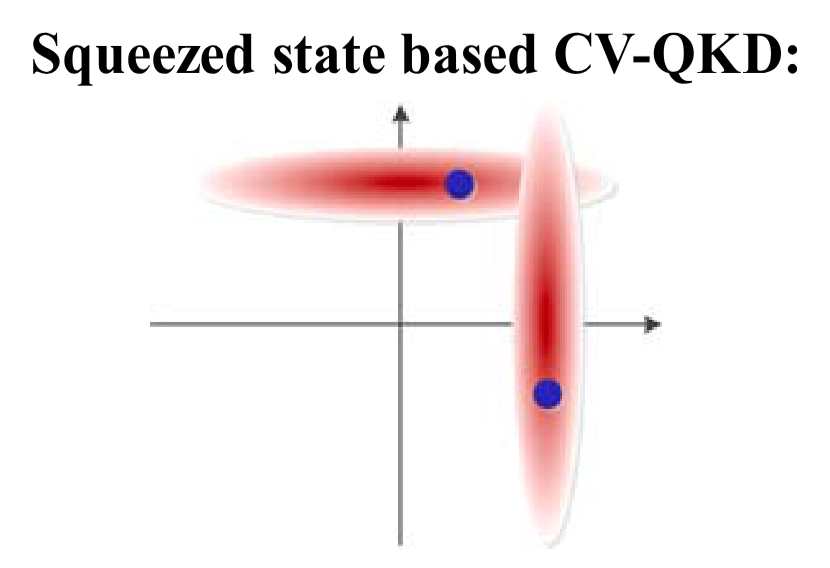
\includegraphics[width=0.42\textwidth]{chapters/figs/fig-6-26-a}}
	\hfill
	\subfigure[\lr{CV-QKD} مبتنی بر حالت همدوس]{\label{fig:6-26-b}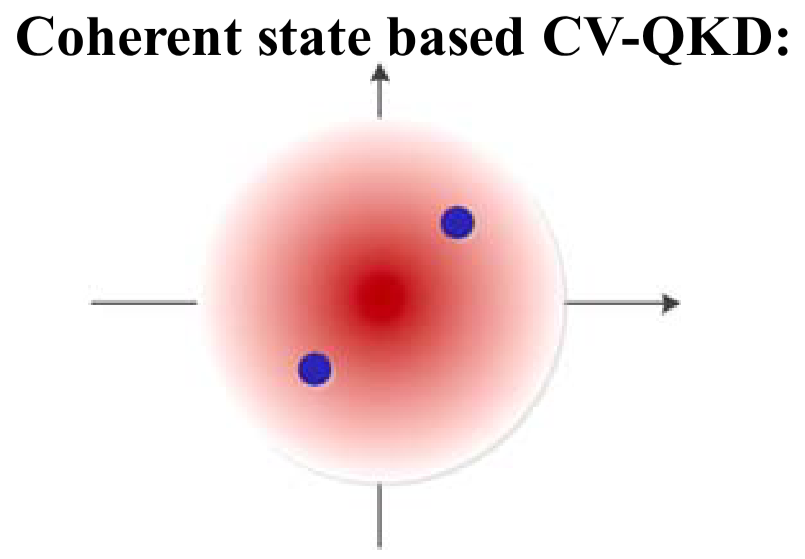
\includegraphics[width=0.42\textwidth]{chapters/figs/fig-6-26-b}}
	\caption{تصویرسازی اصول عملکرد پروتکل‌های مبتنی بر حالت فشرده (\subref{fig:6-26-a}) و همدوس (\subref{fig:6-26-b}).}
	\label{fig:6-26}
\end{figure}


که در آن $f_{\mathcal{N}}(0,s)$ توزیع گاوسی با میانگین صفر و واریانس $s^2$ است. هنگامی که شرط $\rho_I = \rho_Q$ برقرار باشد، ایو نمی‌تواند تشخیص دهد که آلیس اطلاعات را روی حالت فشرده $I$ یا $Q$ اعمال کرده است. با توجه به اینکه تولید حالت‌های فشرده بسیار دشوارتر از حالت‌های همدوس است، تمرکز خود را بر پروتکل‌های \lr{CV-QKD} مبتنی بر حالت همدوس معطوف می‌کنیم.

\subsection{پروتکل‌های توزیع کلید کوانتومی با متغیر پیوسته مبتنی بر حالت همدوس}
\label{subsec:6-10-3}
در پروتکل‌های مبتنی بر حالت همدوس، که اصول عملکرد آن‌ها در شکل \ref{fig:6-26} (\subref{fig:6-26-b}) ارائه شده است، تنها یک قاعده کدگذاری برای آلیس وجود دارد:
\begin{equation}
	X_{A,I}; X_{A,Q} \sim X_{A,I} + jX_{A,Q}; \quad X_{A,I} \sim \mathcal{N}(0, \sqrt{v_A}); \quad X_{A,Q} \sim \mathcal{N}(0, \sqrt{v_A})
	\label{eq:6-81}
\end{equation}
به عبارت دیگر، آلیس با کمک دستگاه ارائه شده در شکل \ref{fig:6-25}، به‌طور تصادفی نقطه‌ای را در فضای دوبعدی ($I,Q$) از یک توزیع گاوسی متقارن دایره‌ای با میانگین صفر انتخاب می‌کند. به‌وضوح، هر دو مؤلفه مربعی دارای عدم قطعیت یکسانی هستند. در اینجا نیز از اصل عدم قطعیت هایزنبرگ استفاده می‌کنیم که بیان می‌دارد اندازه‌گیری هر دو مؤلفه مربعی با دقت کامل غیرممکن است. برای گیرنده هموداین، باب اندازه‌گیری تصادفی را روی $\hat{I}$ یا $\hat{Q}$ انجام می‌دهد؛ فرض کنید نتیجه اندازه‌گیری او با $Y_B$ نشان داده شود. وقتی باب $\hat{I}$ را اندازه‌گیری می‌کند، اندازه‌گیری او ($Y_B$) با $X_{A,I}$ همبسته است. از سوی دیگر، وقتی باب $\hat{Q}$ را اندازه‌گیری می‌کند، نتیجه اندازه‌گیری او ($Y_B$) با $X_{A,Q}$ همبسته است. به‌وضوح، باب قادر است با استفاده از حالت همدوس گاوسی، یک مختصات واحد از نقطه منظومه سیگنال ارسال شده توسط آلیس را اندازه‌گیری کند. سپس باب اعلام می‌کند که در هر بازه سیگنال‌دهی کدام مؤلفه مربعی را اندازه‌گیری کرده است و آلیس مختصاتی را انتخاب می‌کند که با مؤلفه مربعی اندازه‌گیری شده توسط باب مطابقت دارد. باقی پروتکل مشابه پروتکل مبتنی بر حالت فشرده است.

از دیدگاه ایو، حالت مخلوط به‌صورت زیر خواهد بود:
\begin{equation}
	\rho = \int f_{\mathcal{N}}(0, \sqrt{v_A}) f_{\mathcal{N}}(0, \sqrt{v_A}) |I + jQ\rangle \langle I + jQ| dI dQ
	\label{eq:6-82}
\end{equation}
در اینجا $v_A$ واریانس مدولاسیون آلیس در واحد \lr{SNU} است. برای ارسال بدون تلفات، واریانس کل متغیر تصادفی باب در واحد \lr{SNU} به‌صورت زیر خواهد بود:
\begin{equation}
	V(Y_B) = \text{Var}(Y_B) = v_A + 1
	\label{eq:6-83}
\end{equation}
که از جمله مدولاسیون آلیس $v_A$ و واریانس نوسانات ذاتی حالت همدوس (که برابر با $1$ است) تشکیل شده است.

برای ارسال با تلفات\LTRfootnote{Lossy transmission}، کانال را می‌توان به‌صورت یک تقسیم‌کننده پرتو با تضعیف $0 \leq T \leq 1$ مدل‌سازی کرد، همان‌طور که در شکل \ref{fig:6-27} تصویر شده است. از این شکل نتیجه می‌گیریم که حالت خروجی $x_B$ را می‌توان برحسب حالت ورودی $x_A$ و حالت پایه\LTRfootnote{Ground state} $x_0$ به‌صورت زیر نشان داد:
\begin{equation}
	x_B = \sqrt{T} x_A + \sqrt{1-T} x_0 = \sqrt{T} (x_A + \sqrt{\chi_{\text{line}}} x_0); \quad \chi_{\text{line}} = (1-T)/T = 1/T - 1
	\label{eq:6-84}
\end{equation}
برای ارسال با تلفات، زمانی که به جای حالت‌های خلاء از مدولاسیون گاوسی حالت‌های همدوس استفاده می‌شود، رابطه قبلی باید به‌صورت زیر اصلاح گردد:
\begin{equation}
	x_B = \sqrt{T} (x_A + \sqrt{\chi_{\text{line}}} x_0); \quad \chi_{\text{line}} = (1-T)/T + \epsilon = 1/T - 1 + \epsilon; \quad \epsilon \geq 0
	\label{eq:6-85}
\end{equation}
که در آن $\epsilon$ نشان‌دهنده نویز اضافی\LTRfootnote{Excess noise} است.


\begin{figure}[ht]
	\centering
	% \includegraphics[width=0.8\textwidth]{fig6-27}
	\caption{تصویرسازی کانال ارسال با تلفات.}
	\label{fig:6-27}
\end{figure}

نخستین جمله در $\chi_{\text{line}}$ مربوط به تضعیف کانال\LTRfootnote{Channel attenuation} است، در حالی که جمله دوم یعنی $\epsilon$ که معمولاً نویز اضافی\LTRfootnote{Excess noise} نامیده می‌شود، ناشی از سایر عوامل نویزی نظیر نویز فاز لیزر\LTRfootnote{Laser phase noise}، عدم تعامد کامل مؤلفه‌های مربعی و غیره است. واریانس کل متغیر تصادفی باب اکنون شامل سه جمله خواهد بود:
\begin{equation}
	V(Y_B) = \text{Var}(Y_B) = T \left[ \underbrace{v_A + 1}_{v} + \chi_{\text{line}} \right] = T(v + \chi_{\text{line}})
	\label{eq:6-86}
\end{equation}
که در آن $v = v_A + 1$ است. اطلاعات متقابل بین آلیس و باب بر اساس فرمول شانون را می‌توان به‌صورت زیر محاسبه کرد:
\begin{equation}
	I(A; B) \approx I(X_A; Y_B) = \frac{1}{2} \log \left( 1 + \frac{T v_A}{T(1 + \chi_{\text{line}})} \right) = \frac{1}{2} \log \left( 1 + \frac{v_A}{1 + \chi_{\text{line}}} \right)
	\label{eq:6-87}
\end{equation}
اطلاعات ایو در طرح‌های \lr{CV-QKD} توسط استراتژی مصالحه\LTRfootnote{Reconciliation strategy} تعیین می‌شود. با فرض اینکه تمامی منابع نویز اضافی از نظر آماری مستقل و جمع‌شونده\LTRfootnote{Additive} باشند، واریانس کل (در واحد \lr{SNU}) را می‌توان به‌صورت مجموع مشارکت‌های فردی نمایش داد:
\begin{equation}
	\epsilon = \epsilon_{\text{modulator}} + \epsilon_{PN} + \epsilon_{RIN} + \dots
	\label{eq:6-88}
\end{equation}
که در آن جمله نخست نشان‌دهنده نقایص مدولاسیون\LTRfootnote{Modulation imperfections}، جمله دوم متناظر با نویز فاز و جمله سوم متناظر با نویز شدت نسبی\LTRfootnote{Relative intensity noise (RIN)} سیگنال مرجع \lr{LO} است.

اکنون با ارجاع به ورودی باب (یا به‌طور معادل خروجی کانال)، می‌توانیم واریانس نویز آشکارساز معادلِ باب را به‌صورت زیر نمایش دهیم:
\begin{equation}
	\chi_{\text{det}} = \frac{\delta(1 + v_{el}) - \eta}{\eta}
	\label{eq:6-89}
\end{equation}

که در آن برای آشکارسازی هموداین، $\delta = 1$ (در طرح آشکارسازی هموداین، در هر بازه سیگنال‌دهی معین می‌توان مؤلفه هم‌فاز یا مربعی را اندازه‌گیری کرد) و برای \lr{HD}، $\delta = 2$ است (هر دو مؤلفه مربعی را می‌توان به‌طور هم‌زمان اندازه‌گیری کرد). پارامتر $\eta$ نشان‌دهنده بازدهی آشکارسازی است، در حالی که $v_{el}$ نشان‌دهنده واریانس نویز الکتریکی معادل\LTRfootnote{Equivalent electrical noise} است. واریانس نویز کل\LTRfootnote{Total noise} را می‌توان با جمع کردن واریانس نویز کانال و نویز آشکارسازی تعیین کرد، که با ارجاع به ورودی کانال به‌صورت زیر بیان می‌شود:
\begin{equation}
	\chi_{total} = \chi_{line} + \frac{\chi_{det}}{T} = \underbrace{\frac{1-T}{T} + \epsilon}_{\chi_{line}} + \frac{\delta(1+v_{el}) - \eta}{T\eta}
	\label{eq:6-90}
\end{equation}
هنگام ارجاع به خروجی کانال، واریانس نویز کل در سمت باب را می‌توان به‌صورت زیر تعیین کرد:
\begin{equation}
	\begin{aligned}
		\chi_{total, Bob} &= T\eta \left( \chi_{line} + \frac{\chi_{det}}{T} \right) = T\eta \left( \frac{1-T}{T} \right) + T\eta\epsilon + T\eta \left( \frac{\delta(1+v_{el}) - \eta}{T\eta} \right) \\
		&= \eta(1-T) + T\eta\epsilon + \delta(1+v_{el}) - \eta
		\label{eq:6-91}
	\end{aligned}
\end{equation}
برای یک سیستم دوقسمتی\LTRfootnote{Bipartite system} متشکل از دو زیرسیستم جدایی‌پذیر\LTRfootnote{Separable subsystems} $A$ و $B$ که هر یک با ماتریس‌های چگالی متناظر $\rho_A$ و $\rho_B$ توصیف می‌شوند، عملگر چگالی سیستم دوقسمتی را می‌توان به‌صورت $\rho = \rho_A \otimes \rho_B$ نشان داد. برای یک سیستم دوقسمتی گاوسی متشکل از دو زیرسیستم جدایی‌پذیر $A$ و $B$، به‌طوری که زیرسیستم $A$ یک حالت گاوسی با $M$ مُد باشد که با عملگرهای مؤلفه مربعی $\hat{\bm{x}}_A$ بازنمایی می‌شود، و زیرسیستم $B$ یک حالت گاوسی با $N$ مُد باشد که با عملگرهای مؤلفه مربعی $\hat{\bm{x}}_B$ بازنمایی می‌شود؛ حالت گاوسی سیستم دوقسمتی شامل $M+N$ مُد خواهد بود و می‌توان آن را با عملگرهای مؤلفه مربعی $\hat{\bm{x}} = [\hat{\bm{x}}_A, \hat{\bm{x}}_B]^T$ توصیف کرد؛ ماتریس کوواریانس\LTRfootnote{Covariance matrix} متناظر با ابعاد $2(M+N) \times 2(M+N)$ به‌صورت زیر بازنمایی می‌شود:
\begin{equation}
	\bm{S} = \bm{S}_A \oplus \bm{S}_B = \begin{bmatrix} \bm{S}_A & \zeros \\ \zeros & \bm{S}_B \end{bmatrix}
	\label{eq:6-92}
\end{equation}
که در آن $\zeros$ نشان‌دهنده ماتریس تمام‌صفر است.

فرض کنیم حالت \lr{EPR} تعریف‌شده در رابطه \eqref{eq:5-199} در سیستم \lr{CV-QKD} استفاده شود، که ماتریس کوواریانس آن در رابطه \eqref{eq:5-219} تعریف شده است. از ماتریس همانی می‌توان برای توصیف حالت گرمایی\LTRfootnote{Thermal state} در ورودی تقسیم‌کننده پرتو استفاده کرد (شکل \ref{fig:6-27} را ببینید). بر اساس معادله قبلی، سیستم دوقسمتی متناظر دارای ماتریس همبستگی\LTRfootnote{Correlation matrix} زیر خواهد بود:
\begin{equation}
	\bm{S} = \begin{bmatrix} \bm{S}_{EPR} & \zeros \\ \zeros & \ones \end{bmatrix} = \begin{bmatrix} v\ones & \sqrt{v^2-1}\bm{Z} & \zeros \\ \sqrt{v^2-1}\bm{Z} & v\ones & \zeros \\ \zeros & \zeros & \ones \end{bmatrix}
	\label{eq:6-93}
\end{equation}
تقسیم‌کننده پرتو بر روی کیوبیت باب و حالت گرمایی اثر می‌گذارد، در حالی که کیوبیت آلیس را بدون تغییر باقی می‌گذارد؛ بنابراین، عملکرد آن را می‌توان به‌صورت زیر توصیف کرد:

\begin{equation}
	\bm{BS}_{\text{combined}}(T) = \begin{bmatrix} 
		 & \zeros & \zeros \\ 
		\zeros & \sqrt{T}\ones & \sqrt{1-T}\ones \\ 
		\zeros & -\sqrt{1-T}\ones & \sqrt{T}\ones 
	\end{bmatrix} = \begin{bmatrix} 
		1 & 0 & 0 & 0 & 0 & 0 \\
		0 & 1 & 0 & 0 & 0 & 0 \\
		0 & 0 & \sqrt{T} & 0 & \sqrt{1-T} & 0 \\
		0 & 0 & 0 & \sqrt{T} & 0 & \sqrt{1-T} \\
		0 & 0 & -\sqrt{1-T} & 0 & \sqrt{T} & 0 \\
		0 & 0 & 0 & -\sqrt{1-T} & 0 & \sqrt{T}
	\end{bmatrix}
	\label{eq:6-94}
\end{equation}
برای تعیین ماتریس کوواریانس پس از تقسیم‌کننده پرتو، عملگر سیمپلکتیک\LTRfootnote{Symplectic operation} توسط $\bm{BS}_{\text{combined}}$ را بر ماتریس کوواریانس ورودی اعمال می‌کنیم تا $\bm{S}'$ را به‌دست آوریم:
\begin{equation}
	\bm{S}' = \bm{BS}_{\text{combined}}(T) \bm{S} [\bm{BS}_{\text{combined}}(T)]^T
	\label{eq:6-95}
\end{equation}
اکنون با نگه‌داشتن تنها زیرماتریس‌های آلیس و باب، خواهیم داشت:
\begin{equation}
	\bm{S}'_{AB} = \begin{bmatrix} 
		v\ones & \sqrt{T(v^2-1)}\mathbf{Z} \\ 
		\sqrt{T(v^2-1)}\mathbf{Z} & (vT + 1 - T)\ones 
	\end{bmatrix}
	\label{eq:6-96}
\end{equation}
در حضور نویز اضافی\LTRfootnote{Excess noise}، نیاز است که عنصر $(\bm{S}'_{AB})_{22}$ را با $vT + 1 + \epsilon' T$ جایگزین کنیم تا ماتریس کوواریانس زیر برای آشکارسازی هموداین به‌دست آید:
\begin{equation}
	\bm{S}_{AB}^{(\text{homodyne})} = \begin{bmatrix} 
		v\ones & \sqrt{T(v^2-1)}\mathbf{Z} \\ 
		\sqrt{T(v^2-1)}\mathbf{Z} & (vT + 1 + \epsilon' - T)\ones 
	\end{bmatrix}
	\label{eq:6-97}
\end{equation}
در آشکارسازی هتروداین (\lr{HD})، باب از یک \lr{BBS} برای تقسیم سیگنال کوانتومی استفاده می‌کند، در حالی که ورودی دوم به \lr{BBS} حالت خلاء است و عملکرد \lr{BBS} را می‌توان با رابطه \eqref{eq:5-159} و با قرار دادن $T=1/2$ نشان داد. ماتریس کوواریانس متناظر در ورودی \lr{BBS} به‌صورت زیر خواهد بود:
\begin{equation}
	\bm{S}_{\text{in}}^{(\text{BBS})} = \begin{bmatrix} 
		\bm{S}_{AB}^{(\text{homodyne})} & \zeros \\ 
		\zeros & \ones 
	\end{bmatrix}
	\label{eq:6-98}
\end{equation}
ماتریس کوواریانس و خروجی \lr{BBS} را می‌توان با اعمال عملگر سیمپلکتیک توسط $\bm{BS}_{\text{combined}}(1/2)$ بر ماتریس کوواریانس ورودی تعیین کرد تا ماتریس زیر برای حالت هتروداین به‌دست آید:
\begin{align}
	\bm{S}_{AB}^{(\text{het})} &= \bm{BS}_{\text{combined}}(1/2) \bm{S}_{\text{in}}^{(\text{BBS})} [\bm{BS}_{\text{combined}}(1/2)]^T \notag\\&= \begin{bmatrix} 
		v\ones & \sqrt{\frac{T}{2}(v^2-1)}\mathbf{Z} & -\sqrt{\frac{T}{2}(v^2-1)}\mathbf{Z} \\ 
		\sqrt{\frac{T}{2}(v^2-1)}\mathbf{Z} & \frac{vT + 2 + \epsilon' - T}{2}\ones & \frac{vT + \epsilon' - T}{2}\ones \\ 
		-\sqrt{\frac{T}{2}(v^2-1)}\mathbf{Z} & \frac{vT + \epsilon' - T}{2}\ones & \frac{vT + 2 + \epsilon' - T}{2}\ones 
	\end{bmatrix}
	\label{eq:6-99}
\end{align}
همان‌طور که در بخش‌های قبل بحث شد، آلیس به جای استفاده از حالت \lr{EPR}، طرح آماده‌سازی-و-اندازه‌گیری را به کار می‌گیرد که در آن از یک منبع \lr{WCS} استفاده کرده و با کمک یک مدولاتور \lr{I/Q}، حالت گاوسی با واریانس $v_A$ تولید می‌کند. با توجه به اینکه حداقل عدم قطعیت منبع همدوس یک \lr{SNU} است، واریانس باب $v_A + 1$ خواهد بود و می‌توانیم عملگر هم‌فاز باب را به‌صورت زیر نمایش دهیم:
\begin{equation}
	\hat{I}_B \approx \hat{I}_A + \mathcal{N}(0, 1)
	\label{eq:6-100}
\end{equation}
که در آن $\mathcal{N}(0,1)$ یک منبع گاوسی با میانگین صفر و واریانس $1$ \lr{SNU} است. به‌وضوح، واریانس عملگر هم‌فاز باب برابر با $V(\hat{I}_B) = V(\hat{I}_A) + 1 = v_A + 1$ است. از سوی دیگر، کوواریانس عملگرهای هم‌فاز آلیس و باب به‌صورت زیر خواهد بود:
\begin{equation}
	\begin{aligned}
		\text{Cov}(\hat{I}_A, \hat{I}_B) &= \left\langle \left( \hat{I}_A - \underbrace{\langle \hat{I}_A \rangle}_{=0} \right) \left( \hat{I}_B - \underbrace{\langle \hat{I}_B \rangle}_{0} \right) \right\rangle = \left\langle \hat{I}_A \underbrace{\hat{I}_B}_{\hat{I}_A + \mathcal{N}(0,1)} \right\rangle = \langle \hat{I}_A^2 \rangle + \underbrace{\langle \hat{I}_A \mathcal{N}(0,1) \rangle}_{=0} \\
		&= v_A = \text{Cov}(\hat{I}_B, \hat{I}_A).
		\label{eq:6-101}
	\end{aligned}
\end{equation}

بنابراین، ماتریس کوواریانس برای پروتکل آماده‌سازی-و-اندازه‌گیری به‌صورت زیر است:
\begin{equation}
	\begin{aligned}
		\bm{\Sigma}_{AB}^{(\text{PM protocol})} &= \begin{bmatrix} 
			\underbrace{V(\hat{I}_A)\ones}_{v_A \ones} & \underbrace{\text{Cov}(\hat{I}_A, \hat{I}_B)\ones}_{v_A \ones} \\ 
			\underbrace{\text{Cov}(\hat{I}_B, \hat{I}_A)\ones}_{v_A \ones} & \underbrace{V(\hat{I}_B)\ones}_{v_B=v_A+1} 
		\end{bmatrix} \\
		&= \begin{bmatrix} 
			v_A \ones & v_A \ones \\ 
			v_A \ones & \underbrace{(v_A+1)}_{v} \ones 
		\end{bmatrix} = \begin{bmatrix} 
			(v-1) \ones & (v-1) \ones \\ 
			(v-1) \ones & v \ones 
		\end{bmatrix}
		\label{eq:6-102}
	\end{aligned}
\end{equation}

\subsection{نرخ کلید مخفی توزیع کلید کوانتومی با متغیر پیوسته با مدولاسیون گاوسی تحت حملات دسته‌جمعی}
\label{sec:6-10-4}
در این زیربخش، نحوه محاسبه کسر مخفی\LTRfootnote{Secret fraction} برای طرح \lr{CV-QKD} مبتنی بر آشکارسازی هموداین حالت همدوس را در شرایطی که ایو از حمله دسته‌جمعی گاوسی\LTRfootnote{Gaussian collective attack} \cite{131, 132, 133, 134, 135} استفاده می‌کند، شرح می‌دهیم؛ حمله‌ای که به عنوان بهینه‌ترین حالت برای مدولاسیون گاوسی شناخته می‌شود. این حمله به‌طور کامل با تخمین ماتریس کوواریانس $\bm{\Sigma}_{AB}$ توسط آلیس و باب مشخص می‌شود، که بر اساس رابطه \eqref{eq:6-97} برای آشکارسازی هموداین و رابطه \eqref{eq:6-99} برای \lr{HD} است. بیایید ماتریس کوواریانس را برای آشکارسازی هموداین به‌صورت زیر بازنویسی کنیم:
\begin{equation}
	\begin{aligned}
		\bm{\Sigma}_{AB}^{(\text{homodyne})} &= \begin{bmatrix} 
			v \ones & \sqrt{T(v^2-1)} \bm{Z} \\ 
			\sqrt{T(v^2-1)} \bm{Z} & T \left( \underbrace{v + 1/T - 1 + \epsilon'/T}_{\epsilon} \right) \ones 
		\end{bmatrix} \\
		&= \begin{bmatrix} 
			v \ones & \sqrt{T(v^2-1)} \bm{Z} \\ 
			\sqrt{T(v^2-1)} \bm{Z} & T \left( v + \underbrace{1/T - 1 + \epsilon}_{\chi_{\text{line}}} \right) \ones 
		\end{bmatrix} \\
		&= \begin{bmatrix} 
			v \ones & \sqrt{T(v^2-1)} \bm{Z} \\ 
			\sqrt{T(v^2-1)} \bm{Z} & T(v + \chi_{\text{line}}) \ones 
		\end{bmatrix}
		\label{eq:6-103}
	\end{aligned}
\end{equation}
که در آن $\epsilon = \epsilon'/T$ نویز دسترسی\LTRfootnote{Access noise} و $1/T - 1$ جمله تلفات کانال\LTRfootnote{Channel loss term} است که هر دو از سمت آلیس (در ورودی کانال) مشاهده می‌شوند. واریانس کل هر دو جمله با $\chi_{\text{line}} = 1/T - 1 + \epsilon$ نشان داده شده است. اکنون با افزودن جمله نویز آشکارساز، ماتریس کوواریانس برای آشکارسازی هموداین به‌صورت زیر در می‌آید:
\begin{equation}
	\bm{\Sigma}_{AB}^{(\text{hom., complete})} = \begin{bmatrix} 
		v\ones & \sqrt{T\eta(v^2 - 1)}\bm{Z} \\ 
		\sqrt{T\eta(v^2 - 1)}\bm{Z} & T\eta(v + \chi_{\text{total}})\ones 
	\end{bmatrix}, \quad v = v_A + 1
	\label{eq:6-104}
\end{equation}
که در آن $\eta$ بازدهی آشکارسازی\LTRfootnote{Detection efficiency} است و $\chi_{\text{total}}$ پیش‌تر در رابطه \eqref{eq:6-90} تعیین شد؛ یعنی $\chi_{\text{total}} = \chi_{\text{line}} + \chi_{\text{det}}/T = \chi_{\text{line}} + [\delta(1 + v_{el}) - \eta]/(T\eta)$، که در آن $v_{el}$ واریانس نویز الکتریکی معادل\LTRfootnote{Equivalent electrical noise} است.

در \lr{CV-QKD} برای مصالحه مستقیم\LTRfootnote{Direct reconciliation} با نرخ کلید مخفی (\lr{SKR})\LTRfootnote{Secret-key rate (SKR)} غیرصفر، تلفات کانال از پایین به $T \geq 1/2$ محدود می‌شود \cite{2,8} و برای تلفات کانال بالاتر، باید از مصالحه معکوس\LTRfootnote{Reverse reconciliation} استفاده کنیم. در مصالحه معکوس، کسر مخفی\LTRfootnote{Secret fraction} به‌صورت زیر داده می‌شود:
\begin{equation}
	r = \beta I(A; B) - \chi(B; E)
	\label{eq:6-105}
\end{equation}
که در آن $\beta$ بازدهی مصالحه\LTRfootnote{Reconciliation efficiency} و $I(A; B)$ اطلاعات متقابل\LTRfootnote{Mutual information} بین آلیس و باب است که برای هر دو نوع حملات انفرادی و دسته‌جمعی یکسان می‌باشد \cite{2,8}:
\begin{equation}
	I(A; B) = \frac{\delta}{2} \log_2 \left( \frac{v + \chi_{\text{total}}}{1 + \chi_{\text{total}}} \right), \quad \delta = 
	\begin{cases} 
		1, & \text{آشکارسازی هموداین} \\ 
		2, & \text{آشکارسازی هتروداین} 
	\end{cases}
	\label{eq:6-106}
\end{equation}
که چیزی جز فرمول تعریف ظرفیت کانال گاوسی نیست. آنچه برای تعیین باقی می‌ماند، اطلاعات هولِوو\LTRfootnote{Holevo information} بین باب و ایو است که با $\chi(B; E)$ نشان داده می‌شود؛ استخراج این مقدار بسیار چالش‌برانگیزتر است و در ادامه توصیف خواهد شد. پس از آن، \lr{SKR} را می‌توان به‌عنوان حاصل‌ضرب کسر مخفی و نرخ سیگنال‌دهی تعیین کرد. با توجه به اینکه آشکارسازی هموداین/هتروداین با محدودیت زمان مرده\LTRfootnote{Dead time} مواجه نیست، نرخ‌های \lr{SKR} معمول در طرح‌های \lr{CV-QKD} به‌طور قابل‌توجهی بالاتر از طرح‌های \lr{DV-QKD} است.

اطلاعات هولِوو بین ایو و باب را می‌توان به‌صورت زیر محاسبه کرد:
\begin{equation}
	\chi(E; B) = S_E - S_{E|B}
	\label{eq:6-107}
\end{equation}
که در آن $S_E$ آنتروپی فون نویمان\LTRfootnote{von Neumann entropy} عملگر چگالی ایو ($\hat{\rho}_E$) است که به‌صورت زیر تعریف می‌شود:
\begin{equation}
	S(\hat{\rho}_E) = -\text{Tr}(\hat{\rho}_E \log \hat{\rho}_E)
	\label{eq:6-108}
\end{equation}
در حالی که $S_{E|B}$ آنتروپی فون نویمان حالت ایو در زمانی است که باب اندازه‌گیری تصویرگر\LTRfootnote{Projective measurement} (اعم از هموداین یا هتروداین) را انجام می‌دهد. در اصل، مقادیر ویژه سیمپلکتیک\LTRfootnote{Symplectic eigenvalues} ماتریس‌های همبستگی متناظر را می‌توان ابتدا برای محاسبه آنتروپی‌های فون نویمان، مطابق آنچه در بخش \ref{sec:5-8-3} شرح داده شد، تعیین کرد. برای ساده‌سازی تحلیل، معمولاً فرض می‌کنیم که ایو مالک پالایش\LTRfootnote{Purification} حالت مشترک آلیس و باب ($\hat{\rho}_{AB}$) است، به‌طوری که حالت حاصل یک حالت خالص $|\psi\rangle$ بوده و عملگر چگالی متناظر به‌صورت زیر خواهد بود:
\begin{equation}
	\hat{\rho}_{ABE} = |\psi\rangle \langle \psi|
	\label{eq:6-109}
\end{equation}
با گرفتن اثر جزئی\LTRfootnote{Partial trace} روی زیرفضای ایو، حالت مخلوط آلیس-باب را به‌دست می‌آوریم، یعنی $\hat{\rho}_{AB} = \text{Tr}_E \hat{\rho}_{ABE}$. به‌طور مشابه، با گرفتن اثر روی زیرفضای آلیس-باب، حالت مخلوط ایو به‌صورت $\hat{\rho}_E = \text{Tr}_{AB} \hat{\rho}_{ABE}$ به‌دست می‌آید. با به‌کارگیری قضیه تجزیه اشمیت\LTRfootnote{Schmidt decomposition theorem} \cite{2,7,9}، می‌توانیم حالت دوقسمتی\LTRfootnote{Bipartite state} $|\psi\rangle \in \mathcal{H}_{AB} \otimes \mathcal{H}_E$ را برحسب پایه‌های اشمیت برای زیرسیستم $AB$ (نشان داده شده با $\{|i_{AB}\rangle\}$) و زیرسیستم $E$ (نشان داده شده با $\{|i_E\rangle\}$) به‌صورت زیر نمایش دهیم:
\begin{equation}
	|\psi\rangle = \sum_i \sqrt{p_i} |i_{AB}\rangle |i_E\rangle
	\label{eq:6-110}
\end{equation}

که در آن $\sqrt{p_i}$ ضرایب اشمیت\LTRfootnote{Schmidt coefficients} هستند که در رابطه $\sum_i p_i = 1$ صدق می‌کنند. با گرفتن اثر جزئی\LTRfootnote{Tracing out} روی زیرسیستم ایو، عملگر چگالی مخلوط\LTRfootnote{Mixed density operator} زیر برای زیرسیستم آلیس-باب به‌دست می‌آید:
\begin{equation}
	\hat{\rho}_{AB} = \text{Tr}_E (|\psi\rangle\langle\psi|) = \sum_i p_i |i_{AB}\rangle\langle i_{AB}|.
	\label{eq:6-111}
\end{equation}
از سوی دیگر، با گرفتن اثر جزئی روی زیرسیستم آلیس-باب، حالت مخلوط زیر برای ایو حاصل می‌شود:
\begin{equation}
	\hat{\rho}_E = \text{Tr}_{AB} (|\psi\rangle\langle\psi|) = \sum_i p_i |i_E\rangle\langle i_E|.
	\label{eq:6-112}
\end{equation}
به‌وضوح، عملگرهای چگالی آلیس-باب و ایو دارای طیف (مقادیر ویژه) یکسانی هستند و بنابراین، آنتروپی فون نویمان\LTRfootnote{von Neumann entropy} یکسانی دارند:
\begin{equation}
	S_{AB} = S_E = -\sum_i p_i \log p_i.
	\label{eq:6-113}
\end{equation}
اکنون محاسبه اطلاعات هولِوو بسیار ساده می‌شود، زیرا رابطه زیر برقرار است:
\begin{equation}
	\chi(E; B) = S_E - S_{E|B} = S_{AB} - S_{A|B}.
	\label{eq:6-114}
\end{equation}
برای تعیین آنتروپی فون نویمان زیرسیستم آلیس-باب که مستقل از اندازه‌گیری باب است، از ماتریس کوواریانس زیر (برگرفته از رابطه \eqref{eq:6-104}) که در ورودی کانال مشاهده می‌شود، استفاده می‌کنیم:
\begin{equation}
	\bm{\Sigma}_{AB} = \begin{bmatrix} 
		v\ones & \sqrt{T(v^2-1)}\bm{Z} \\ 
		\sqrt{T(v^2-1)}\bm{Z} & T(v + \chi_{\text{line}})\ones 
	\end{bmatrix}.
	\label{eq:6-115}
\end{equation}
برای تعیین مقادیر ویژه سیمپلکتیک\LTRfootnote{Symplectic eigenvalues}، از تئوری بخش‌های \ref{sec:5-8-4} و \ref{sec:5-8-6} استفاده می‌کنیم. به‌وضوح، ماتریس کوواریانس دارای شکلی مشابه با رابطه \eqref{eq:5-200} است، به‌طوری که در آن $a=v$، $b=T(v + \chi_{\text{line}})$ و $c=\sqrt{T(v^2-1)}$ است. می‌توان مستقیماً از رابطه \eqref{eq:5-201} برای تعیین مقادیر ویژه سیمپلکتیک استفاده کرد. متناوباً، با توجه به اینکه مقادیر ویژه سیمپلکتیک در روابط زیر صدق می‌کنند:
\begin{equation}
	\lambda_1^2 + \lambda_2^2 = a^2 + b^2 - 2c^2; \quad \lambda_1^2 \lambda_2^2 = (ab - c^2)^2,
	\label{eq:6-116}
\end{equation}
با معرفی متغیرهای زیر:
\begin{equation}
	\begin{aligned}
		A &= a^2 + b^2 - 2c^2 = v^2(1 - 2T) + 2T + T^2(v + \chi_{\text{line}})^2, \\
		B &= (ab - c^2)^2 = T^2(1 + v\chi_{\text{line}})^2,
		\label{eq:6-117}
	\end{aligned}
\end{equation}
مقادیر ویژه سیمپلکتیک متناظر برای ماتریس کوواریانس آلیس-باب را می‌توان به‌صورت زیر بیان کرد:
\begin{equation}
	\lambda_{1,2} = \sqrt{\frac{1}{2} (A \pm \sqrt{A^2 - 4B})},
	\label{eq:6-118}
\end{equation}
که نشان‌دهنده شکلی است که اغلب در متون علمی یافت می‌شود \cite{129, 130, 131, 150, 151}. آنتروپی فون نویمان بر اساس قضیه تجزیه حالت گرمایی\LTRfootnote{Thermal state decomposition theorem} و رابطه \eqref{eq:5-195} به‌صورت زیر داده می‌شود:
\begin{equation}
	S_{AB} = S(\hat{\rho}_{AB}) = g\left(\frac{\lambda_1 - 1}{2}\right) + g\left(\frac{\lambda_2 - 1}{2}\right).
	\label{eq:6-119}
\end{equation}	

محاسبه $S_{A|B}$ به استراتژی اندازه‌گیری باب، یعنی هموداین یا هتروداین، بستگی دارد و می‌توانیم تئوری اندازه‌گیری‌های جزئی\LTRfootnote{Partial measurements} از بخش \ref{sec:5-8-5} را به کار ببریم. برای آشکارسازی هموداین، بر اساس رابطه \eqref{eq:5-214}، نتیجه می‌گیریم که $\bm{A} = v\ones$، $\bm{B} = T(v+\chi_{\text{line}})\ones$ و $\bm{C} = \sqrt{T(v^2 - 1)}\bm{Z}$ است، به‌طوری که اندازه‌گیری هموداینِ باب، ماتریس کوواریانس بالا را به‌صورت زیر تبدیل می‌کند:
\begin{equation}
	\bm{\Sigma}_{A|B}^{(\hat{I})} = \bm{A} - \frac{1}{V(\hat{I})} \bm{C} \bm{\Pi}_I \bm{C}^T = \begin{bmatrix} v - \frac{v^2-1}{v+\chi_{\text{line}}} & 0 \\ 0 & v \end{bmatrix}.
	\label{eq:6-120}
\end{equation}
مقدار ویژه سیمپلکتیک اکنون با حل رابطه زیر تعیین می‌شود:
\begin{equation}
	\det(j\bm{\Omega}\bm{\Sigma}_{A|B} - \lambda\ones) = \lambda^2 + v \left( \frac{v^2-1}{v+\chi_{\text{line}}} - v \right) = 0,
	\label{eq:6-121}
\end{equation}
و با حل برای $\lambda$، به‌دست می‌آوریم:
\begin{equation}
	\lambda_3 = \sqrt{v \left( v - \frac{v^2-1}{v+\chi_{\text{line}}} \right)};
	\label{eq:6-122}
\end{equation}
بنابراین $S_{A|B}$ به $g(\lambda_3)$ تبدیل می‌شود. این عبارت با آنچه در مرجع \cite{150} ارائه شده مطابقت دارد، با این تفاوت که از ماتریس همبستگی کمی متفاوتی استفاده شده بود. در نهایت، برای آشکارسازی هموداین، اطلاعات هولِوو به‌صورت زیر داده می‌شود:
\begin{equation}
	\chi(E; B) = S_{AB} - S_{A|B} = g\left(\frac{\lambda_1 - 1}{2}\right) + g\left(\frac{\lambda_2 - 1}{2}\right) - g\left(\frac{\lambda_3 - 1}{2}\right).
	\label{eq:6-123}
\end{equation}
در \lr{HD}، باب هر دو مؤلفه مربعی را اندازه‌گیری می‌کند و با توجه به اینکه یک \lr{BBS} اضافی با یک ورودی در حالت خلاء استفاده شده است، باید نوسانات ناشی از حالت خلاء را لحاظ کرده و ماتریس همبستگی جزئی را طبق مراجع \cite{2, 147} به‌صورت زیر اصلاح کنیم:
\begin{equation}
	\bm{\Sigma}_{A|B} = \bm{A} - \bm{C}(\bm{B} + \ones)^{-1}\bm{C}^T = K\ones, \quad K = v - \frac{T(v^2 - 1)}{T(v + \chi_{\text{line}}) + 1}.
	\label{eq:6-124}
\end{equation}
مقدار ویژه سیمپلکتیک را می‌توان از معادله مشخصه\LTRfootnote{Characteristic equation} زیر تعیین کرد:
\begin{equation}
	\det(j\bm{\Omega}\bm{\Sigma}_{A|B}^{(\text{heterodyne})} - \lambda\ones) = \lambda^2 - K^2 = 0,
	\label{eq:6-125}
\end{equation}
تا مقدار زیر به‌دست آید:
\begin{equation}
	\lambda_3^{(\text{heterodyne})} = K = v - \frac{T(v^2 - 1)}{T(v + \chi_{\text{line}}) + 1}.
	\label{eq:6-126}
\end{equation}
در نهایت، برای \lr{HD}، اطلاعات هولِوو به‌صورت زیر داده می‌شود:
\begin{equation}
	\chi(E; B)^{(\text{heterodyne})} = g\left(\frac{\lambda_1 - 1}{2}\right) + g\left(\frac{\lambda_2 - 1}{2}\right) - g\left(\frac{\lambda_3^{(\text{heterodyne})} - 1}{2}\right).
	\label{eq:6-127}
\end{equation}

\subsection{نتایج مصالحه معکوس برای توزیع کلید کوانتومی با متغیر پیوسته مبتنی بر مدولاسیون گاوسی}
\label{sec:6-10-5}
این بخش با به‌کارگیری مشتقات ارائه‌شده در زیربخش قبل، کسر مخفی\LTRfootnote{Secrecy fraction} توصیفی (نرخ‌های کلید مخفی (\lr{SKR})\LTRfootnote{Secret-key rate (SKR)} نرمالیزه‌شده) را برای سناریوهای مختلف ارائه می‌دهد. ما تنها موارد مصالحه معکوس\LTRfootnote{Reverse reconciliation} را در نظر می‌گیریم. در شکل \ref{fig:6-28}، نرخ‌های \lr{SKR} نرمالیزه‌شده در مقابل تلفات کانال، در حالی که واریانس نویز الکتریکی برحسب \lr{SNU}\LTRfootnote{Shot-noise unit (SNU)} به عنوان پارامتر در نظر گرفته شده است، ارائه می‌شوند. واریانس نویز اضافی\LTRfootnote{Excess noise variance} بر روی $\epsilon = 10^{-3}$، بازدهی آشکارساز\LTRfootnote{Detector efficiency} بر روی $\eta = 0.85$ و بازدهی مصالحه\LTRfootnote{Reconciliation efficiency} بر روی $\beta = 0.85$ تنظیم شده است. جالب اینجاست که وقتی واریانس نویز الکتریکی $v_{el} \leq 0.1$ باشد، افت چندانی در \lr{SKR}ها مشاهده نمی‌شود؛ این امر نشان می‌دهد که فتودتکتورهای \lr{p.i.n.} موجود در بازار را می‌توان در \lr{CV-QKD} به کار برد.

در شکل \ref{fig:6-29}، نرخ‌های \lr{SKR} نرمالیزه‌شده در مقابل تلفات کانال نشان داده شده است، در حالی که واریانس نویز اضافی (بیان‌شده برحسب \lr{SNU}) به عنوان پارامتر استفاده می‌شود. واریانس نویز الکتریکی بر روی $v_{el} = 10^{-2}$، بازدهی آشکارساز بر روی $\eta = 0.85$ و بازدهی مصالحه بر روی $\beta = 0.85$ تنظیم شده است. به‌وضوح، واریانس نویز اضافی تأثیر زیادی بر عملکرد \lr{SKR} دارد.

در شکل \ref{fig:6-30}، نرخ‌های \lr{SKR} نرمالیزه‌شده را در مقابل تلفات کانال ارائه می‌دهیم، در حالی که بازدهی آشکارساز $\eta$ به عنوان پارامتر در نظر گرفته شده است. واریانس نویز اضافی بر روی $\epsilon = 10^{-3}$، واریانس نویز الکتریکی بر روی $v_{el} = 10^{-2}$ و بازدهی مصالحه بر روی $\beta = 0.85$ تنظیم شده است. مشخصاً، بازدهی آشکارسازی تأثیر زیادی بر \lr{SKR}ها ندارد.

در شکل \ref{fig:6-31}، نرخ‌های \lr{SKR} نرمالیزه‌شده را در مقابل تلفات کانال نشان می‌دهیم، در حالی که بازدهی مصالحه $\beta$ به عنوان پارامتر استفاده شده است. واریانس نویز اضافی بر روی $\epsilon = 10^{-3}$، واریانس نویز الکتریکی بر روی $v_{el} = 10^{-2}$ و بازدهی آشکارساز بر روی $\eta = 0.85$ تنظیم شده است. بدیهی است که بازدهی مصالحه تأثیر قابل‌توجهی بر \lr{SKR}ها دارد.

\begin{figure}[ht]
	\centering
	 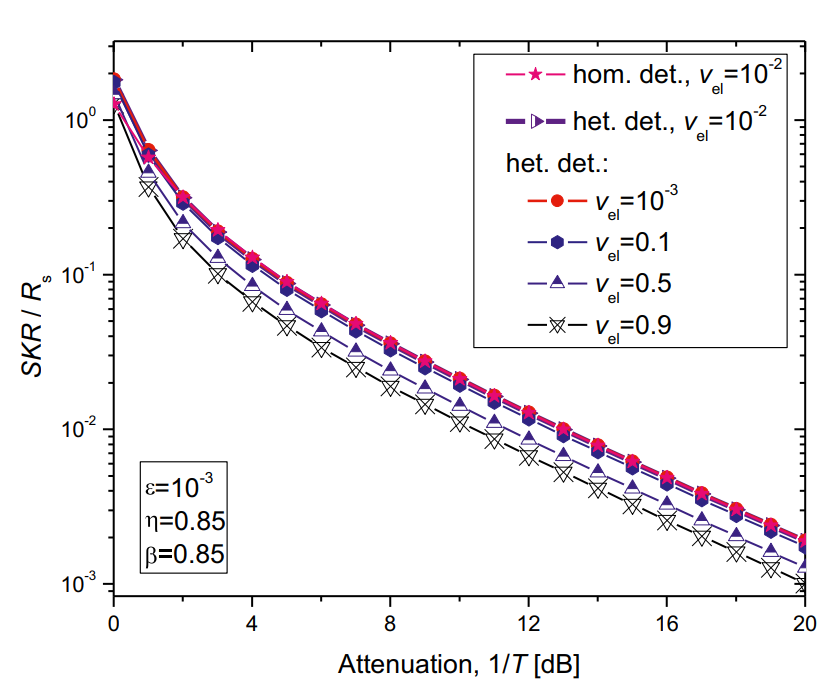
\includegraphics[width=0.7\textwidth]{chapters/figs/fig-6-28}
	\caption{کسر مخفی برای طرح توزیع کلید کوانتومی با متغیر پیوسته با مدولاسیون گاوسی برحسب تلفات کانال در شرایطی که واریانس نویز الکتریکی یک پارامتر است.}
	\label{fig:6-28}
\end{figure}

\begin{figure}[ht]
	\centering
	 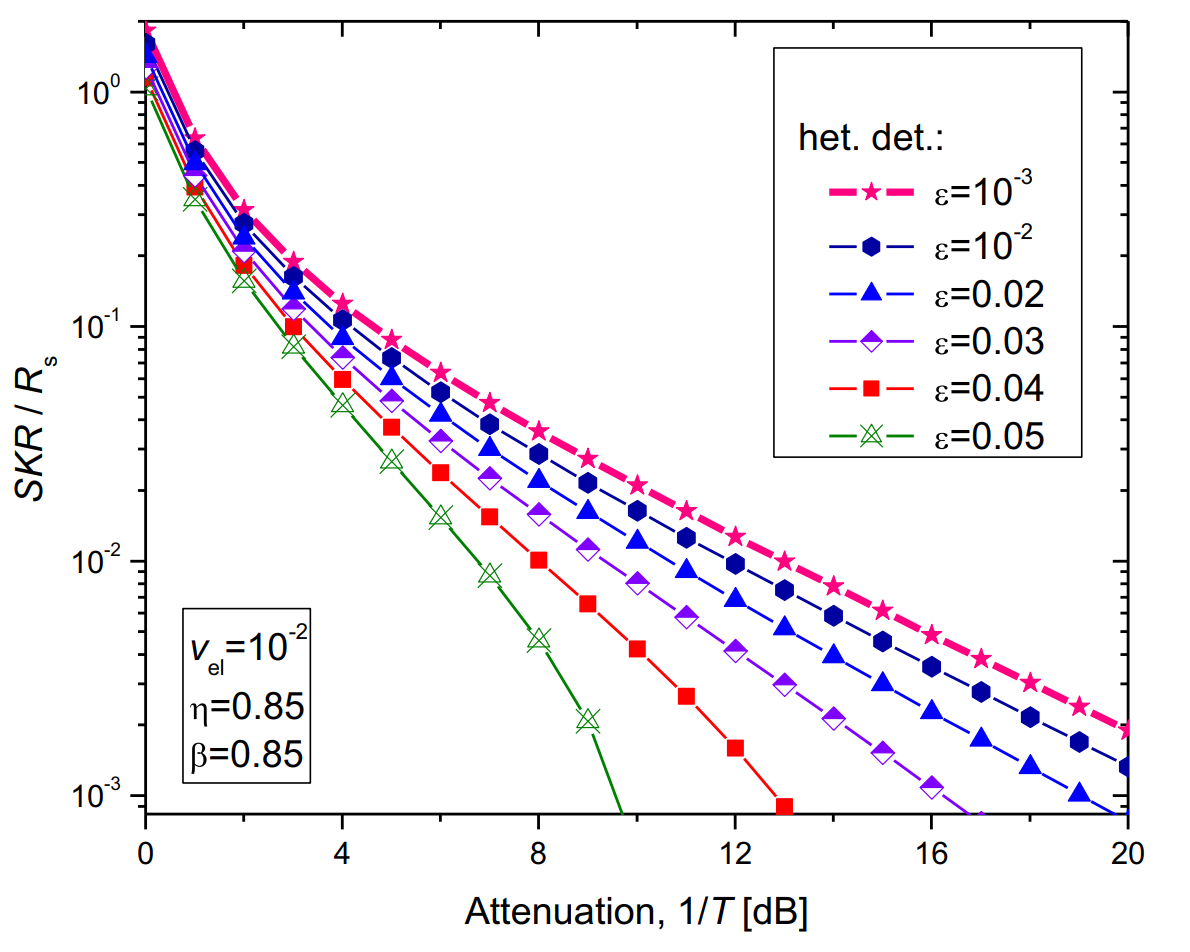
\includegraphics[width=0.7\textwidth]{chapters/figs/fig-6-29}
	\caption{کسر مخفی برای طرح توزیع کلید کوانتومی با متغیر پیوسته با مدولاسیون گاوسی برحسب تلفات کانال در شرایطی که واریانس نویز اضافی یک پارامتر است.}
	\label{fig:6-29}
\end{figure}

\begin{figure}[ht]
	\centering
	 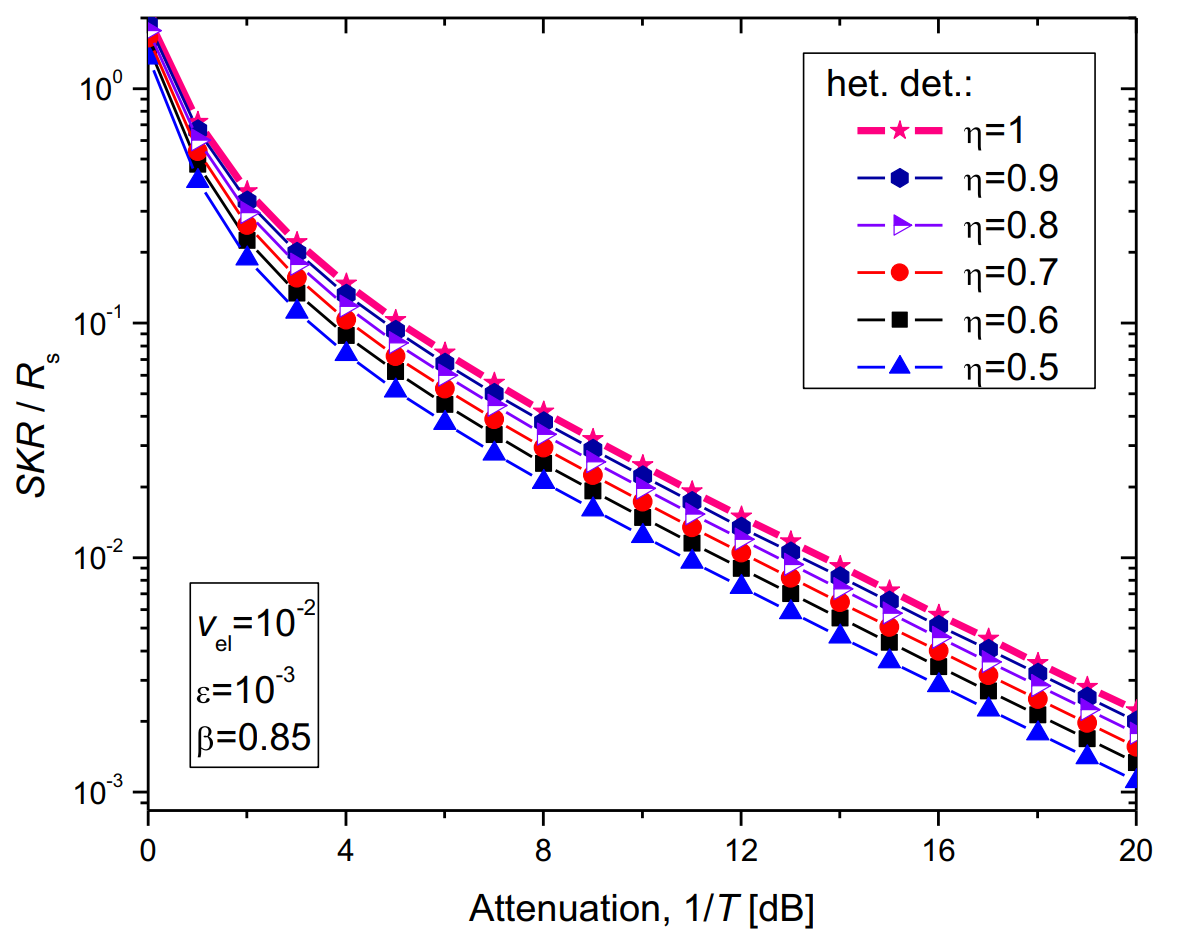
\includegraphics[width=0.7\textwidth]{chapters/figs/fig-6-30}
	\caption{کسر مخفی برای طرح توزیع کلید کوانتومی با متغیر پیوسته با مدولاسیون گاوسی برحسب تلفات کانال در شرایطی که بازدهی آشکارساز یک پارامتر است.}
	\label{fig:6-30}
\end{figure}

\section{خلاصه}
\label{sec:6-11}
این فصل به مفاهیم بنیادی \lr{QKD} اختصاص یافت. تفاوت‌های اصلی بین رمزنگاری متداول و \lr{QKD} در بخش \ref{sec:6-1} تشریح شد. در بخش مبانی \lr{QKD} (بخش \ref{sec:6-2})، پس از یک مرور تاریخی، انواع مختلف \lr{QKD} به‌اختصار معرفی شدند. بخش \ref{sec:6-3} به توصیف دو قضیه بنیادی پرداخت که \lr{QKD} بر آن‌ها استوار است؛ یعنی قضیه کپی‌ناپذیری و قضیه عدم توانایی در تمایز ابهام‌ناپذیر حالت‌های کوانتومی غیرمتعامد. در بخش \ref{sec:6-4}، مربوط به سیستم‌های \lr{DV-QKD}، پروتکل‌های \lr{BB84}، \lr{B92}، اکرت (\lr{E91})، \lr{EPR} و کدگذاری فاز-زمان در زیربخش‌های متناظر \ref{subsec:6-4-1} تا \ref{sec:6-4-4} شرح داده شدند. بخش \ref{sec:6-5} به امنیت \lr{QKD} اختصاص داشت که در آن \lr{SKR} به‌عنوان حاصل‌ضرب کلید خام و نرخ‌های کسری نمایش داده می‌شود. علاوه بر این، عبارت عمومی برای نرخ کسری ارائه شد و به‌دنبال آن استراتژی‌های مختلف شنود، از جمله حملات انفرادی (بخش \ref{subsec:6-5-1})، دسته‌جمعی (بخش \ref{subsec:6-5-2}) و حملات هک کوانتومی/کانال جانبی (بخش \ref{subsec:6-5-3}) توصیف شدند. برای حملات انفرادی و همدوس، عبارات کسر مخفی متناظر ارائه شد که شامل کسر مخفی برای پروتکل \lr{BB84} در بخش \ref{subsec:6-5-4} بود. در بخش \ref{sec:6-6}، پروتکل حالت فریب همراه با محاسبات \lr{SKR} مربوطه تشریح گردید.

\begin{figure}[ht]
	\centering
	 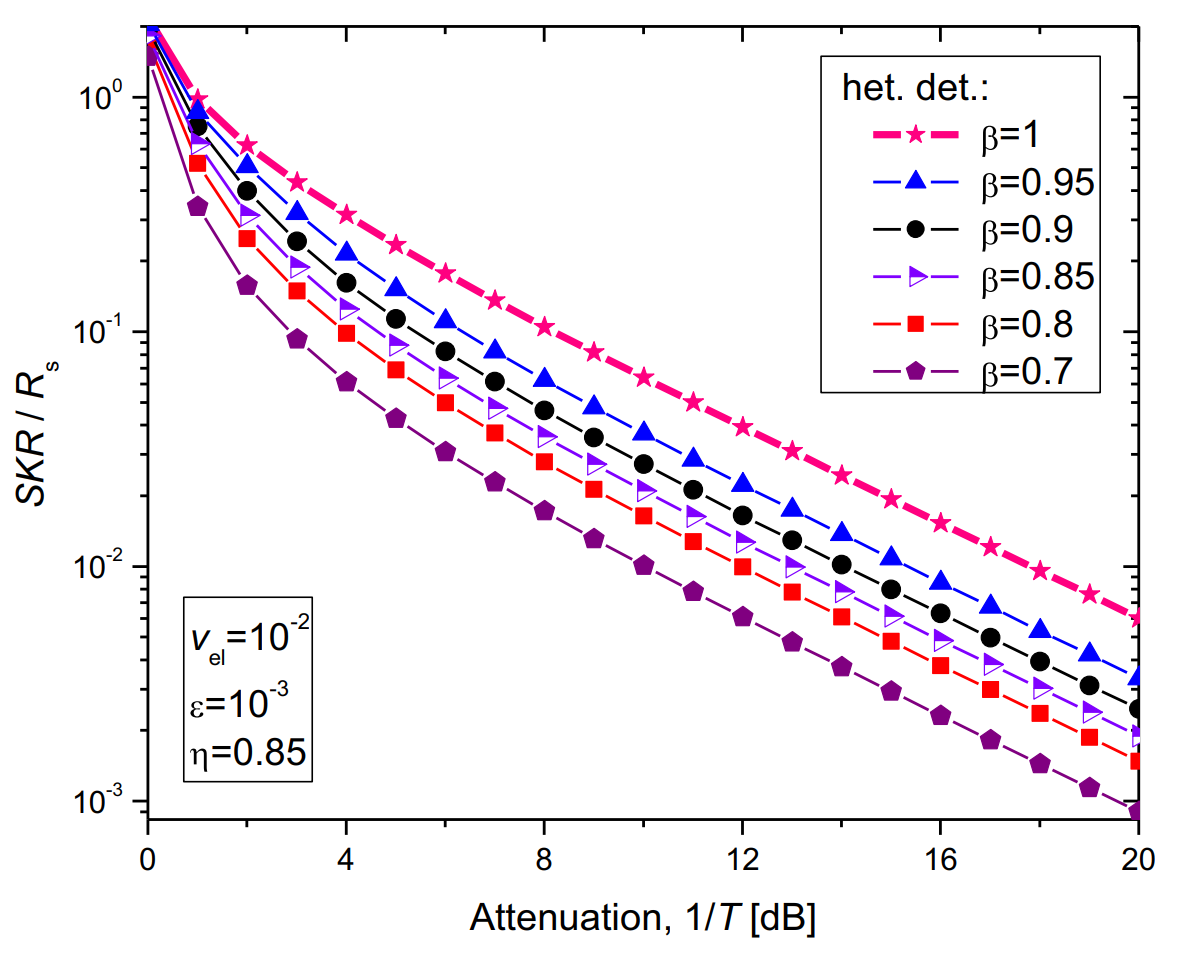
\includegraphics[width=0.7\textwidth]{chapters/figs/fig-6-31}
	\caption{کسر مخفی برای طرح توزیع کلید کوانتومی با متغیر پیوسته با مدولاسیون گاوسی برحسب تلفات کانال در شرایطی که بازدهی مصالحه یک پارامتر است.}
	\label{fig:6-31}
\end{figure}

مفاهیم کلیدی پروتکل \lr{MDI-QKD} در بخش \ref{sec:6-7} معرفی شدند که شامل \lr{BSM}های فوتونی (بخش \ref{subsec:6-7-1})، پروتکل \lr{MDI-QKD} مبتنی بر قطبش (بخش \ref{subsec:6-7-2}) و پروتکل \lr{MDI-QKD} مبتنی بر کدگذاری فاز-زمان (بخش \ref{subsec:6-7-3}) بود، در حالی که محاسبات کسر مخفی در بخش \ref{subsec:6-7-4} ارائه گردید. پروتکل‌های \lr{TF-QKD} در بخش \ref{sec:6-8} بیشتر تشریح شدند و عملکرد آن‌ها در برابر پروتکل‌های حالت فریب و \lr{MDI-QKD} ارزیابی شد. در بخش \ref{sec:6-9}، بحث به سمت مراحل پردازش کلاسیک، شامل گام‌های مصالحه اطلاعات (بخش \ref{sec:6-9-1}) و تقویت حریم خصوصی (بخش \ref{sec:6-9-2}) حرکت کرد.

بخش \ref{sec:6-10} به پروتکل‌های \lr{CV-QKD} اختصاص یافت که در آن طرح‌های آشکارسازی هموداین و هتروداین در بخش \ref{subsec:6-10-1}، پس از شرح مختصری از پروتکل‌های مبتنی بر حالت فشرده در بخش \ref{sec:6-10-2}، توصیف شدند. با توجه به اینکه تولید و دست‌کاری حالت‌های همدوس بسیار ساده‌تر است، پروتکل‌های مبتنی بر حالت همدوس به‌تفصیل در بخش \ref{subsec:6-10-3} شرح داده شدند. برای یک کانال ارسال با تلفات، ماتریس‌های کوواریانس متناظر برای طرح‌های آشکارسازی همدوس هموداین و هتروداین استخراج گردید و به‌دنبال آن، استخراج \lr{SKR} برای \lr{CV-QKD} مبتنی بر مدولاسیون گاوسی آماده‌سازی-و-اندازه‌گیری در بخش \ref{sec:6-10-4} انجام شد. برخی از نتایج مصالحه توصیفی در بخش \ref{sec:6-10-5} مربوط به طرح‌های \lr{CV-QKD} مبتنی بر مدولاسیون گاوسی ارائه گردید.



























	\chapter{}\chapter{}\chapter{}
	% !TeX root = ../quantum.tex

\chapter{مبانی توزیع کلید کوانتومی (\lr{QKD})}
\label{chap:7}

\section*{چکیده}
این فصل به مبانی توزیع کلید کوانتومی (\lr{QKD}) اختصاص یافته است. فصل با توصیف تفاوت‌های کلیدی بین رمزنگاری متداول\LTRfootnote{Conventional cryptography}، امنیت لایه فیزیکی (\lr{PLS}) کلاسیک و \lr{QKD} آغاز می‌شود. در بخش مبانی \lr{QKD}، پس از یک مرور تاریخی، انواع مختلف \lr{QKD} را بررسی کرده و به‌اختصار مراحل معمول پس‌پردازش\LTRfootnote{Postprocessing}، یعنی مراحل مصالحه اطلاعات\LTRfootnote{Information reconciliation} و تقویت حریم خصوصی\LTRfootnote{Privacy amplification} را شرح می‌دهیم. در همان بخش، دو قضیه بنیادی را که \lr{QKD} بر آن‌ها استوار است ارائه می‌دهیم: قضیه کپی‌ناپذیری\LTRfootnote{No-cloning theorem} و قضیه عدم توانایی در تمایز ابهام‌ناپذیر حالت‌های کوانتومی غیرمتعامد\LTRfootnote{Non-orthogonal quantum states}. در بخش سیستم‌های \lr{QKD} با متغیر گسسته\LTRfootnote{Discrete variable (DV)} (\lr{DV-QKD})، پروتکل‌های \lr{BB84} و \lr{B92} و همچنین پروتکل‌های اکرت (\lr{E91}) و \lr{EPR} را به‌تفصیل توصیف می‌کنیم. در همان بخش، پروتکل کدگذاری فاز-زمان\LTRfootnote{Time-phase encoding} نیز شرح داده شده است. در رابطه با پروتکل‌های \lr{BB84}، نسخه‌های مختلف مناسب برای فناوری‌های گوناگون بررسی می‌شوند. در بخش امنیت \lr{QKD}، نرخ کلید مخفی\LTRfootnote{Secret-key rate (SKR)} (\lr{SKR}) به‌صورت حاصل‌ضرب نرخ کلید خام\LTRfootnote{Raw key rate} و نرخ کسری\LTRfootnote{Fractional rate} نمایش داده شده و به‌دنبال آن محدودیت‌های مختلف نرخ کلید خام توصیف می‌شوند. سپس، عبارت عمومی برای نرخ کسری ارائه شده و انواع استراتژی‌های شنود\LTRfootnote{Eavesdropping strategies}، شامل حملات انفرادی (مستقل یا غیرهمدوس)\LTRfootnote{Individual (independent or incoherent) attacks}، حملات دسته‌جمعی\LTRfootnote{Collective attacks}، حملات همدوس\LTRfootnote{Coherent attacks} و حملات هک کوانتومی/کانال جانبی\LTRfootnote{Quantum hacking/side-channel attacks} تشریح می‌گردند. برای حملات انفرادی و همدوس، عبارات کسر مخفی متناظر شرح داده شده‌اند. بخش بعدی به تعاریف مختلف امنیت، از جمله مفهوم $\epsilon$-امنیت\LTRfootnote{$\epsilon$-security} اختصاص یافته است. سپس، عبارات عمومی برای طرح‌های \lr{DV-QKD} دوبعدی برای هر دو پروتکل آماده‌سازی-و-اندازه‌گیری\LTRfootnote{Prepare-and-measure} و پروتکل‌های مبتنی بر حالت‌های فریب\LTRfootnote{Decoy states} استخراج می‌شوند. برای تسهیل توصیف پروتکل‌های \lr{QKD} با متغیر پیوسته\LTRfootnote{Continuous variable (CV)} (\lr{CV-QKD})، ابتدا مبانی اپتیک کوانتومی\LTRfootnote{Quantum optics} معرفی می‌شوند. در بخش پروتکل‌های \lr{CV-QKD}، هر دو نوع پروتکل مبتنی بر حالت‌های فشرده\LTRfootnote{Squeezed states} و حالت‌های همدوس\LTRfootnote{Coherent states} تشریح می‌شوند. با توجه به اینکه تولید و دست‌کاری حالت‌های همدوس بسیار ساده‌تر است، پروتکل‌های مبتنی بر حالت همدوس با هر دو نوع آشکارسازی هموداین و هتروداین\LTRfootnote{Homodyne and heterodyne detections} به‌تفصیل شرح داده شده‌اند. کسر مخفی برای هر دو پروتکل \lr{CV-QKD} مبتنی بر مصالحه مستقیم و معکوس استخراج شده است. علاوه بر این، جزئیات جنبه‌های کاربردی پروتکل \lr{GG02} ارائه شده و محاسبه کسر مخفی برای حملات دسته‌جمعی مورد بحث قرار گرفته است. سپس، مفاهیم پایه پروتکل‌های \lr{QKD} مستقل از دستگاه اندازه‌گیری\LTRfootnote{Measurement-device-independent (MDI)} (\lr{MDI-QKD}) معرفی می‌شوند. بخش پایانی ملاحظات پایانی مرتبط را ارائه می‌دهد.






\section{از رمزنگاری متداول تا \lr{QKD}}
\label{sec:7-1}

سیستم رمزنگاری\LTRfootnote{Cryptographic system} پایه مبتنی بر کلید در شکل \ref{fig:11-1} ارائه شده است. منبع، پیام (متن‌آشکار\LTRfootnote{Plaintext}) $M$ را به سمت بلوک رمزگذاری\LTRfootnote{Encryption} ارسال می‌کند که این بلوک با کمک کلید $K$ دریافت شده از منبع کلید، رمزنگاشت\LTRfootnote{Cryptogram} را تولید می‌نماید. در سمت گیرنده، رمزنگاشت ارسال شده از طریق کانال ناامن، توسط الگوریتم رمزگشایی\LTRfootnote{Decryption} به همراه کلید $K$ که از طریق کانال امن دریافت شده است، پردازش می‌شود که متن‌آشکار اصلی را برای تحویل به کاربر احرازهویت‌شده\LTRfootnote{Authenticated user} بازسازی می‌کند. فرآیند رمزگذاری را می‌توان به‌صورت ریاضی با $E_K(M) = C$ توصیف کرد، در حالی که فرآیند رمزگشایی با $D_K(C) = M$ بیان می‌شود. مشابه قبل، ترکیب توابع رمزگشایی و رمزگذاری منجر به نگاشت همانی\LTRfootnote{Identity mapping} $D_K(E_K(M)) = M$ می‌گردد. منبع کلید معمولاً کلید را به‌صورت تصادفی از فضای کلید\LTRfootnote{Keyspace} (محدوده مقادیر ممکن برای کلید) تولید می‌کند.

الگوریتم‌های مبتنی بر کلید را می‌توان به دو دسته کلی تقسیم کرد:
\begin{itemize}
	\item \textbf{الگوریتم‌های متقارن\LTRfootnote{Symmetric algorithms}:} که در آن‌ها کلید رمزگشایی را می‌توان از کلید رمزگذاری مشتق کرد و بالعکس. متناوباً، می‌توان از یک کلید یکسان برای هر دو مرحله رمزگذاری و رمزگشایی استفاده کرد. الگوریتم‌های متقارن با نام‌های الگوریتم‌های تک‌کلیدی\LTRfootnote{One-key (single-key) algorithms} یا کلید‌مخفی\LTRfootnote{Secret-key algorithms} نیز شناخته می‌شوند. سیستم شناخته‌شده‌ای که از این نوع الگوریتم استفاده می‌کند، استاندارد رمزگذاری دیجیتال\LTRfootnote{Digital encryption standard (DES)} (\lr{DES}) است \cite{7-1, 7-2, 7-3}.
	\item \textbf{الگوریتم‌های نامتقارن\LTRfootnote{Asymmetric algorithms}:} که در آن‌ها کلیدهای رمزگذاری و رمزگشایی متفاوت هستند. علاوه بر این، کلید رمزگشایی را نمی‌توان در یک بازه زمانی معقول از روی کلید رمزگذاری تعیین کرد. به دلیل این واقعیت، کلیدهای رمزگذاری حتی می‌توانند به‌صورت عمومی منتشر شوند، به‌طوری که یک شنودگر قادر به تعیین کلید رمزگشایی نباشد. سیستم‌های کلید عمومی\LTRfootnote{Public-key systems} \cite{7-4} بر پایه این مفهوم بنا شده‌اند. در سیستم‌های کلید عمومی، کلیدهای رمزگذاری به‌صورت عمومی منتشر می‌شوند، در حالی که کلید رمزگشایی تنها برای کاربر موردنظر شناخته شده است. در این حالت، کلید رمزگذاری را کلید عمومی\LTRfootnote{Public key} و کلید رمزگشایی را کلید مخفی (خصوصی)\LTRfootnote{Secret (private) key} می‌نامند. این کلیدها را می‌توان با هر ترتیبی برای ایجاد رمزنگاشت از متن‌آشکار و بازسازی متن‌آشکار از رمزنگاشت به کار برد.
\end{itemize}

\begin{figure}[H]
	\centering
	 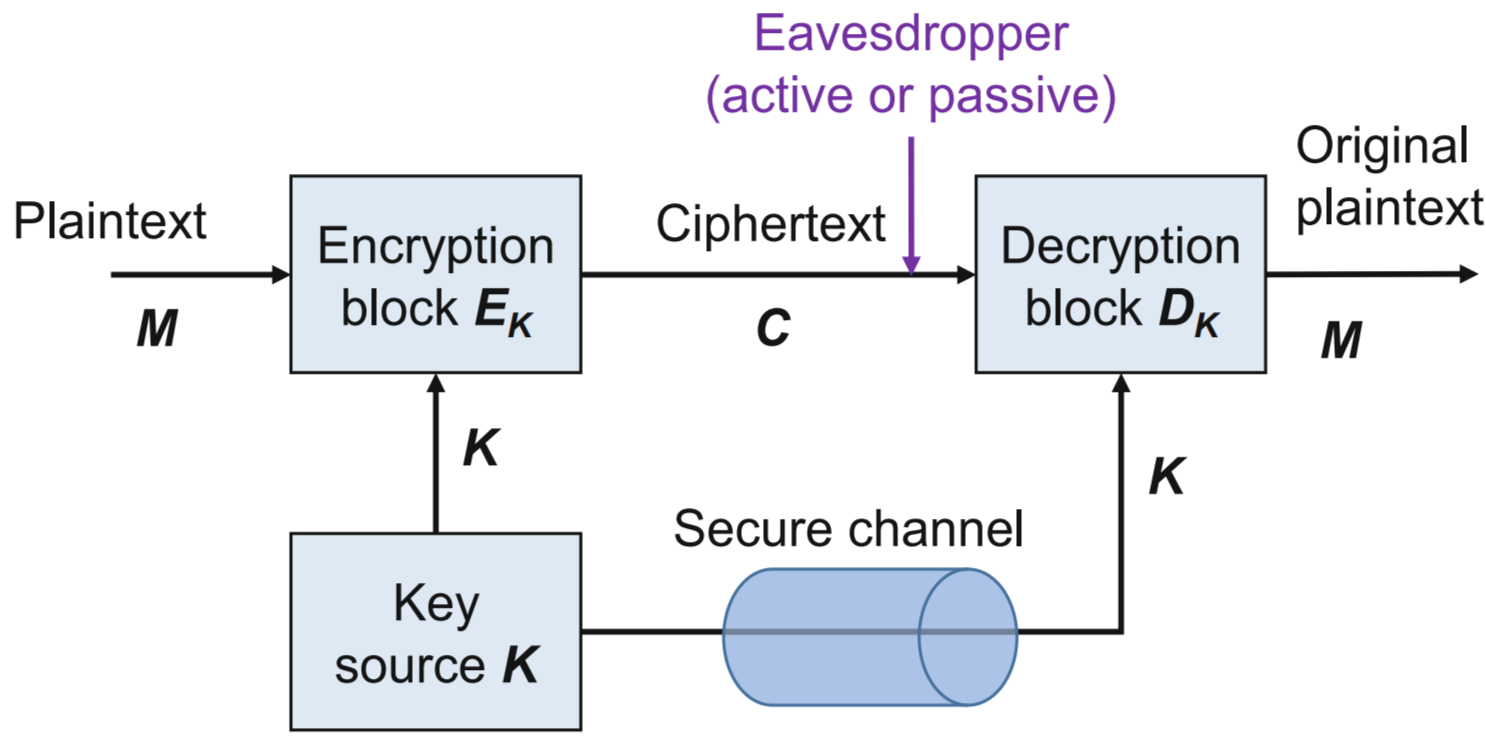
\includegraphics[width=0.7\textwidth]{chapters/figs/fig-7-1}
	\caption{طرح رمزنگاری پایه مبتنی بر کلید.}
	\label{fig:7-1}
\end{figure}






ساده‌ترین سیستم رمزنگاری کلید خصوصی، رمز ورنام\LTRfootnote{Vernam cipher} (پد یک‌بار مصرف\LTRfootnote{One-time pad}) است. در پد یک‌بار مصرف \cite{7-5}، یک دنباله کاملاً تصادفی از نویسه‌ها\LTRfootnote{Characters}، با طولی برابر با طول دنباله پیام، به‌عنوان کلید استفاده می‌شود. هنگامی که برای هر پیام جدید از یک دنباله تصادفی دیگر به‌عنوان کلید استفاده شود، طرح پد یک‌بار مصرف \textit{امنیت کامل}\LTRfootnote{Perfect security} را فراهم می‌کند که در فصل‌های \ref{chap:3} و \ref{chap:4} مورد بحث قرار گرفت. به بیان دقیق‌تر، رویکرد جستجوی جامع\LTRfootnote{Brute-force search} مستلزم بررسی $m^n$ کلید احتمالی است که در آن $m$ اندازه الفبای به‌کار رفته و $n$ طول رمزنگاشتِ شنود شده است. در عمل، در ارتباطات دیجیتال و کامپیوتری، ما معمولاً در الفبای باینری $\mathrm{GF}(2) = \{0, 1\}$ عمل می‌کنیم. برای به‌دست آوردن کلید، به یک مولد تصادفی خاص نیاز داریم و برای رمزگذاری با استفاده از طرح پد یک‌بار مصرف، صرفاً عمل جمع در پیمانه ۲، یعنی عملیات \lr{XOR}، را مطابق شکل \ref{fig:7-2} انجام می‌دهیم. اگرچه طرح پد یک‌بار مصرف امنیت کامل را ارائه می‌دهد، اما چندین نقص دارد \cite{7-6, 7-7, 7-8}: این طرح مستلزم توزیع امن کلید است، طول کلید باید حداقل به اندازه پیام باشد، بیت‌های کلید نمی‌توانند مجدداً استفاده شوند، کلیدها باید پیش از موعد تحویل داده شوند، تا زمان استفاده به‌صورت امن ذخیره گردند و پس از استفاده نابود شوند.

\begin{figure}[ht]
	\centering
	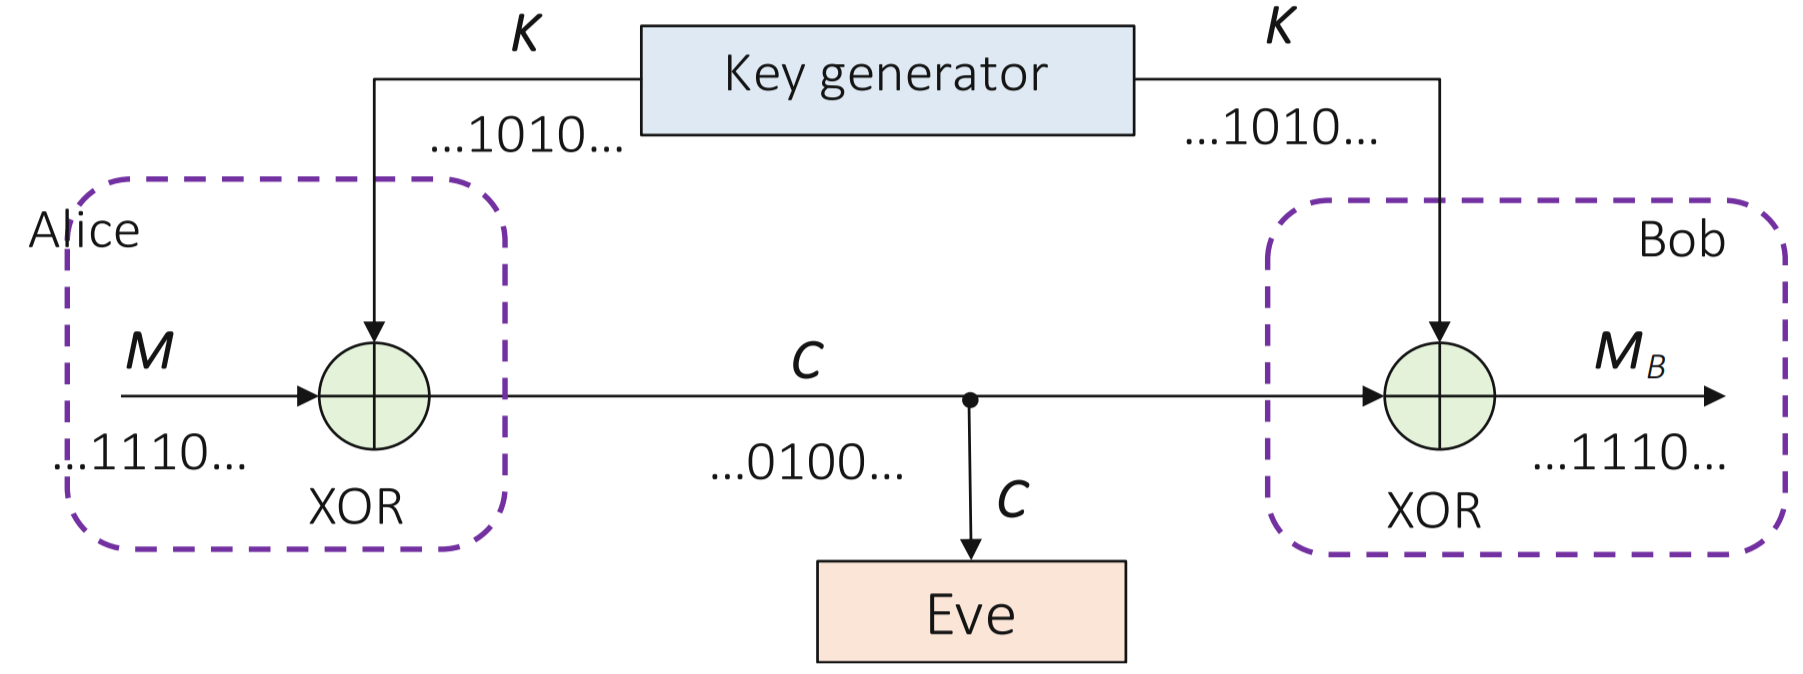
\includegraphics[width=0.8\textwidth]{chapters/figs/fig-7-2}
	\caption{طرح رمزگذاری پد یک‌بار مصرف.}
	\label{fig:7-2}
\end{figure}



طبق گفته شانون \cite{7-9}، امنیت کامل\LTRfootnote{Perfect security} که با نام امنیت غیرمشروط\LTRfootnote{Unconditional security} نیز شناخته می‌شود، زمانی حاصل می‌گردد که پیام‌های $\bm{M}$ و رمزنگاشت‌های $\bm{C}$ از نظر آماری مستقل باشند، به‌طوری که اطلاعات متقابل\LTRfootnote{Mutual information} متناظر برابر با صفر شود:
\begin{equation}
	I(\bm{M}, \bm{C}) = H(\bm{M}) - H(\bm{M}|\bm{C}) = 0 \Leftrightarrow H(\bm{M}|\bm{C}) = H(\bm{M})
	\label{eq:7-1}
\end{equation}
بنابراین، شرط محرمانگی کامل را می‌توان به‌صورت زیر خلاصه کرد:
\begin{equation}
	H(\bm{M}) \leq H(\bm{K}).
	\label{eq:7-2}
\end{equation}
به عبارت دیگر، برای اینکه یک طرح رمزگذاری از امنیت کامل برخوردار باشد، آنتروپی\LTRfootnote{Entropy} (عدم قطعیت\LTRfootnote{Uncertainty}) کلید نمی‌تواند کمتر از آنتروپی پیام باشد. با توجه به اینکه در رمز ورنام طول کلید حداقل برابر با طول پیام است، به نظر می‌رسد طرح پد یک‌بار مصرف دارای امنیت کامل باشد.

با این حال، از آنجا که برآورده کردن این شرط دشوار است، در رمزنگاری متداول به جای امنیت نظریه-اطلاعاتی\LTRfootnote{Information-theoretic security}، از امنیت محاسباتی\LTRfootnote{Computational security} استفاده می‌شود \cite{7-1, 7-3, 7-7, 7-10, 7-11, 7-12}. امنیت محاسباتی دو مورد تعدیل\LTRfootnote{Relaxation} را نسبت به امنیت نظریه-اطلاعاتی معرفی می‌کند \cite{7-3}:










\begin{itemize}
	\item امنیت در برابر یک شنودگر کارآمد\LTRfootnote{Efficient eavesdropper} که حملات تحلیل رمز\LTRfootnote{Cryptanalytic attacks} را برای مدت زمان مشخص و محدودی اجرا می‌کند، تضمین می‌شود. البته، در صورتی که شنودگر منابع محاسباتی کافی و/یا زمان کافی در اختیار داشته باشد، قادر خواهد بود امنیت طرح رمزگذاری را بشکند.
	\item شنودگران می‌توانند در شکستن پروتکل‌های امنیتی موفق شوند، اما با احتمال موفقیت ناچیز.
\end{itemize}
خواننده علاقه‌مند به یادگیری بیشتر درباره امنیت محاسباتی به کتاب ارزشمند کاتز\LTRfootnote{Katz} و لیندل\LTRfootnote{Lindell} \cite{7-3} ارجاع داده می‌شود. با این حال، با استفاده از محاسبات کوانتومی، هر طرح رمزنگاری متداول را می‌توان در بازه زمانی معقولی با به‌کارگیری الگوریتم تجزیه شور\LTRfootnote{Shor's factorization algorithm} \cite{7-13, 7-14, 7-15, 7-16, 7-17} شکست.

\section{مبانی \lr{QKD}}
\label{sec:7-2}
اخیراً دستاوردهای قابل‌توجهی در محاسبات کوانتومی حاصل شده است \cite{7-6, 7-7, 7-8}. بسیاری از شرکت‌ها در حال حاضر مشغول توسعه کامپیوترهای کوانتومی با مقیاس متوسط هستند. با توجه به اینکه اکثر سیستم‌های رمزنگاری به فرض دشواری محاسباتی\LTRfootnote{Computational hardness assumption} وابسته هستند، محاسبات کوانتومی چالشی جدی برای سیستم‌های امنیت سایبری\LTRfootnote{Cybersecurity} مدرن محسوب می‌شود. به‌عنوان یک مثال توصیفی، برای شکستن پروتکل ریواست-شامیر-ادلمن (\lr{RSA}) \cite{7-18}، همان‌طور که در فصل \ref{chap:3} بحث شد، باید دوره تناوب $r$ تابع $f(x) = m^x \pmod n = f(x+r)$ را تعیین کرد (به‌طوری که $r = 0, 1, \dots, 2^{l-1}$ و $m$ یک عدد صحیح کوچک‌تر از $n-1$ است). این دوره تناوب در یکی از مراحل الگوریتم تجزیه شور تعیین می‌شود \cite{7-6, 7-7, 7-8, 7-15, 7-16, 7-17}.








توزیع کلید کوانتومی (\lr{QKD}) با رمزگذاری متقارن را می‌توان به‌عنوان یکی از طرح‌های امنیت لایه فیزیکی\LTRfootnote{Physical-layer security} تفسیر کرد که می‌تواند امنیت اثبات‌پذیر\LTRfootnote{Provable security} را در برابر حملات آغاز شده توسط کامپیوترهای کوانتومی فراهم کند \cite{7-19}. نخستین طرح \lr{QKD} توسط بنت\LTRfootnote{Bennett} و براسارد\LTRfootnote{Brassard} معرفی شد که آن را در سال $1984$ پیشنهاد دادند \cite{7-13, 7-14} و امروزه با نام پروتکل \lr{BB84} شناخته می‌شود. امنیت \lr{QKD} توسط قوانین مکانیک کوانتومی\LTRfootnote{Quantum mechanics laws} تضمین می‌شود. درجات آزادی\LTRfootnote{Degrees of freedom (DOF)} مختلف فوتون، مانند قطبش، زمان، فرکانس، فاز و تکانه زاویه‌ای مداری\LTRfootnote{Orbital angular momentum (OAM)} (\lr{OAM}) را می‌توان برای پیاده‌سازی پروتکل‌های مختلف \lr{QKD} به کار گرفت. به‌طور کلی، بسته به استراتژی اعمال شده در سمت باب، دو طرح کلی \lr{QKD} وجود دارد: \lr{QKD} با متغیر گسسته\LTRfootnote{Discrete variable (DV)} (\lr{DV-QKD}) و \lr{QKD} با متغیر پیوسته\LTRfootnote{Continuous variable (CV)} (\lr{CV-QKD}). در طرح‌های \lr{DV-QKD}، یک آشکارساز تک‌فوتون\LTRfootnote{Single-photon detector (SPD)} (\lr{SPD}) در سمت باب به کار می‌رود، در حالی که در \lr{CV-QKD} مولفه‌های مربعی میدان\LTRfootnote{Field quadratures} با کمک آشکارسازی هموداین/هتروداین\LTRfootnote{Homodyne/heterodyne detection} اندازه‌گیری می‌شوند. طرح \lr{DV-QKD} با به‌کارگیری قضیه کپی‌ناپذیری و قضیه تمایزناپذیری حالت‌های کوانتومی دلخواه\LTRfootnote{Indistinguishability of arbitrary quantum states} به امنیت غیرمشروط\LTRfootnote{Unconditional security} دست می‌یابد که پیش‌تر در فصل \ref{chap:5} اثبات شده‌اند. قضیه کپی‌ناپذیری بیان می‌کند که حالت‌های کوانتومی دلخواه را نمی‌توان کپی کرد، که نشان می‌دهد ایو نمی‌تواند حالت‌های کوانتومی غیرمتعامد\LTRfootnote{Non-orthogonal states} را حتی با کمک کامپیوتر کوانتومی بازتولید کند. از سوی دیگر، قضیه دوم بیان می‌کند که حالت‌های غیرمتعامد را نمی‌توان به‌طور ابهام‌ناپذیر متمایز کرد. به‌ویژه، هنگامی که ایو با حالت‌های کوانتومی ارسالی تعامل برقرار می‌کند تا اطلاعاتی درباره بیت‌های ارسالی به‌دست آورد، به‌طور ناخواسته وفاداری\LTRfootnote{Fidelity} حالت‌های کوانتومی را مختل می‌کند که توسط باب شناسایی خواهد شد. از طرف دیگر، \lr{CV-QKD} از اصل عدم قطعیت\LTRfootnote{Uncertainty principle} بهره می‌برد که بیان می‌کند هر دو مولفه هم‌فاز\LTRfootnote{In-phase} و مربعی حالت‌های همدوس\LTRfootnote{Coherent states} را نمی‌توان به‌طور هم‌زمان با دقت کامل اندازه‌گیری کرد. ما همچنین می‌توانیم طرح‌های مختلف \lr{QKD} را به دو نوع «به کمک درهم‌تنیدگی»\LTRfootnote{Entanglement-assisted} یا «آماده‌سازی-و-اندازه‌گیری»\LTRfootnote{Prepare-and-measure} طبقه‌بندی کنیم.

پژوهش در \lr{QKD} در حال شتاب گرفتن است، به‌ویژه پس از اولین نمایش \lr{QKD} ماهواره به زمین\LTRfootnote{Satellite-to-ground} \cite{7-20}. اخیراً، \lr{QKD} در مسافت $404$ کیلومتری از فیبر نوری با تلفات بسیار کم\LTRfootnote{Ultralow-loss optical fiber} نمایش داده شده است؛ با این حال، این سیستم نرخ کلید امن بسیار پایینی ($3.2 \times 10^{-4}$ بیت بر ثانیه) داشت. با توجه به اینکه حالت‌های کوانتومی قابل تقویت نیستند، تضعیف فیبر مسافت را محدود می‌کند. از سوی دیگر، زمان مرده\LTRfootnote{Deadtime} (مدت زمانی که در آن یک \lr{SPD} به دلیل زمان بازیابی طولانی، نسبت به فوتون‌های ورودی پاسخگو نیست) در \lr{SPD}ها که معمولاً در محدوده $10$ تا $100$ نانوثانیه است، نرخ باود\LTRfootnote{Baud rate} و در نتیجه نرخ کلید امن را محدود می‌کند. طرح‌های \lr{CV-QKD}، از آنجا که از آشکارسازی هموداین/هتروداین استفاده می‌کنند، محدودیت زمان مرده ندارند؛ اما مسافت‌های معمول آن‌ها کوتاه‌تر است.

آلیس و باب با ارسال حالت‌های کیوبیت غیرمتعامد بین خود و بررسی اختلال در حالت ارسالی ناشی از کانال یا فعالیت ایو، می‌توانند حد بالایی برای نویز یا شنود در کانال ارتباطی کوانتومی خود تعیین کنند \cite{7-6}. آستانه حداکثر نرخ خطای تحمل‌پذیر\LTRfootnote{Maximum tolerable error rate} توسط بازدهی بهترین مراحل مصالحه اطلاعات\LTRfootnote{Information reconciliation} و تقویت حریم خصوصی\LTRfootnote{Privacy amplification} تعیین می‌شود \cite{7-6}.




\subsection{انواع سیستم‌های \lr{QKD}}
\label{subsec:7-2-1}
پروتکل‌های \lr{QKD} را می‌توان به چندین دسته کلی تقسیم کرد:
\begin{itemize}
	\item \textbf{\lr{QKD} وابسته به دستگاه\LTRfootnote{Device-dependent QKD}:} که در آن معمولاً منبع کوانتومی در سمت آلیس و آشکارساز کوانتومی در سمت باب قرار می‌گیرد. کلاس‌های محبوب آن عبارتند از: \lr{QKD} با متغیر گسسته (\lr{DV-QKD})، \lr{QKD} با متغیر پیوسته (\lr{CV-QKD})، \lr{QKD} به کمک درهم‌تنیدگی\LTRfootnote{Entanglement-assisted (EA) QKD} (\lr{EA-QKD}) و مرجع فاز توزیع‌شده\LTRfootnote{Distributed phase reference}. در \lr{EA-QKD}، منبع درهم‌تنیده را می‌توان در میانه کانال قرار داد تا مسافت ارسال افزایش یابد.
	\item \textbf{\lr{QKD} مستقل از دستگاه منبع\LTRfootnote{Source-device-independent QKD}:} که در آن منبع کوانتومی در سمت چارلی (ایو) قرار می‌گیرد، در حالی که آشکارسازهای کوانتومی در هر دو سمت آلیس و باب هستند.
	\item \textbf{\lr{QKD} مستقل از دستگاه اندازه‌گیری\LTRfootnote{Measurement-device-independent QKD (MDI-QKD)} (\lr{MDI-QKD}):} که در آن آشکارسازهای کوانتومی در سمت چارلی (ایو) قرار دارند، در حالی که منابع کوانتومی در هر دو سمت آلیس و باب مستقر هستند. حالت‌های کوانتومی در هر دو سمت آلیس و باب آماده‌سازی شده و به سمت آشکارسازهای چارلی ارسال می‌شوند. چارلی اندازه‌گیری‌های حالت بل\LTRfootnote{Bell state measurements} جزئی را انجام داده و زمانی که حالت بل جزئی مورد نظر شناسایی شد، آن را اعلام می‌کند؛ جزئیات مربوطه در ادامه ارائه خواهد شد.
\end{itemize}








\subsection{مراحل مصالحه اطلاعات و تقویت حریم خصوصی}
\label{sec:7-2-2}

مراحل پس‌پردازش کلاسیک\LTRfootnote{Classical postprocessing} در شکل \ref{fig:7-3} خلاصه شده است \cite{7-8}.

\begin{figure}[ht]
	\centering
	 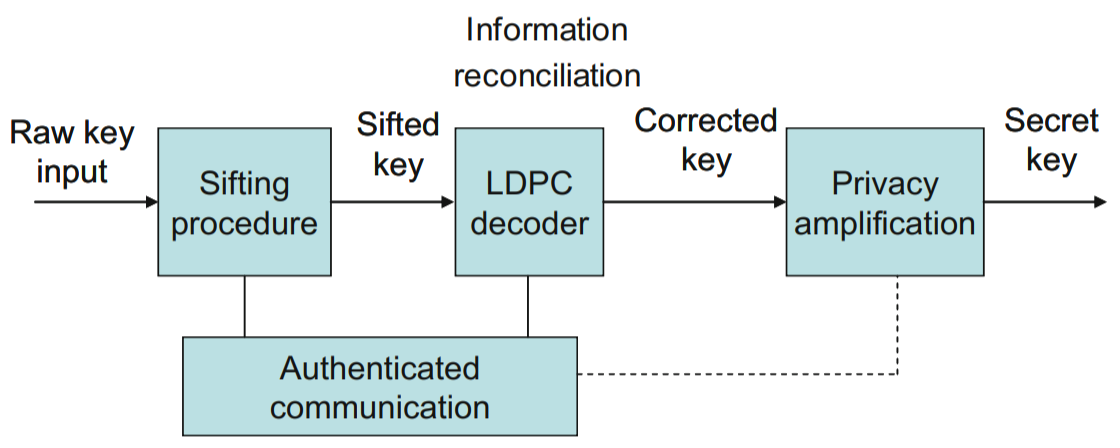
\includegraphics[width=0.8\textwidth]{chapters/figs/fig-7-3}
	\caption{مراحل پس‌پردازش کلاسیک.}
	\label{fig:7-3}
\end{figure}

کلید خام\LTRfootnote{Raw key} ناقص است و ما باید مراحل مصالحه اطلاعات\LTRfootnote{Information reconciliation} و تقویت حریم خصوصی\LTRfootnote{Privacy amplification} را انجام دهیم تا همبستگی بین رشته‌های دنباله $X$ (تولید شده توسط آلیس) و دنباله $Y$ (دریافت شده توسط باب) را افزایش دهیم و در عین حال، اطلاعات متقابل\LTRfootnote{Mutual information} شنودگر (ایو) درباره نتیجه را تا سطح امنیت مطلوب کاهش دهیم.

مصالحه اطلاعات چیزی جز تصحیح خطا\LTRfootnote{Error correction} نیست که روی یک کانال عمومی\LTRfootnote{Public channel} انجام می‌شود و خطاها را بین $X$ و $Y$ مصالحه می‌کند تا یک رشته بیت مشترک $K$ به‌دست آید، در حالی که اطلاعات فاش‌شده برای ایو تا حد امکان کمینه باشد.

تقویت حریم خصوصی \cite{7-21, 7-22} بین آلیس و باب برای استخراج\LTRfootnote{Distill} مجموعه کوچک‌تری از بیت‌ها $S$ از $K$ استفاده می‌شود که همبستگی آن با رشته ایو $Z$ زیر آستانه مطلوب باشد. یکی از راه‌های انجام تقویت حریم خصوصی، استفاده از توابع هش سراسری\LTRfootnote{Universal hash functions} $G$ است که مجموعه رشته‌های $n$-بیتی $A$ را به مجموعه رشته‌های $m$-بیتی $B$ نگاشت می‌کنند، به‌طوری که برای هر دو رشته متمایز $a_1, a_2 \in A$، وقتی $g$ به‌صورت یکنواخت و تصادفی از $G$ انتخاب شود، احتمال برقراری $g(a_1) = g(a_2)$ حداکثر $1/|B|$ باشد.











\subsubsection{قضیه کپی‌ناپذیری و تمایز حالت‌های کوانتومی}
\label{subsec:7-2-3}

\begin{theorem}
	\label{thm:7-1}
	\textit{قضیه کپی‌ناپذیری:} هیچ کپی‌کننده کوانتومی\LTRfootnote{Quantum copier} وجود ندارد که بتواند یک حالت کوانتومی دلخواه\LTRfootnote{Arbitrary quantum state} را کپی کند.
\end{theorem}

\begin{proof}
	اگر حالت ورودی $|\psi\rangle$ باشد، خروجی کپی‌کننده $|\psi\rangle|\psi\rangle$ خواهد بود. برای یک حالت کوانتومی دلخواه، وجود چنین کپی‌کننده‌ای منجر به یک تناقض بنیادی می‌شود.
	دو حالت دلخواه $|\psi\rangle$ و $|\chi\rangle$ را در نظر بگیرید که به‌عنوان ورودی به کپی‌کننده داده می‌شوند. هنگامی که این حالت‌ها به‌صورت مجزا وارد شوند، انتظار داریم خروجی‌های $|\psi\rangle|\psi\rangle$ و $|\chi\rangle|\chi\rangle$ را به‌دست آوریم. اکنون برهم‌نهی\LTRfootnote{Superposition} این دو حالت را به‌صورت زیر در نظر بگیرید:
	\begin{equation}
		\begin{aligned}
			|\phi\rangle = \alpha |\psi\rangle + \beta |\chi\rangle \implies |\phi\rangle |\phi\rangle &= (\alpha |\psi\rangle + \beta |\chi\rangle)(\alpha |\psi\rangle + \beta |\chi\rangle) \\
			&= \alpha^2 |\psi\rangle |\psi\rangle + \alpha\beta |\psi\rangle |\chi\rangle + \alpha\beta |\chi\rangle |\psi\rangle + \beta^2 |\chi\rangle |\chi\rangle
		\end{aligned}
		\label{eq:7-3}
	\end{equation}
	از سوی دیگر، خطی بودن\LTRfootnote{Linearity} مکانیک کوانتومی به ما می‌گوید که کپی‌کننده کوانتومی را می‌توان با یک عملگر یکانی\LTRfootnote{Unitary operator} نمایش داد که عمل کپی کردن را انجام می‌دهد. اگر چنین عملگر یکانی بر روی حالت برهم‌نهی $|\phi\rangle$ اثر کند، خروجی برهم‌نهیِ $|\psi\rangle|\psi\rangle$ و $|\chi\rangle|\chi\rangle$ خواهد بود؛ یعنی:
	\begin{equation}
		|\phi'\rangle = \alpha |\psi\rangle |\psi\rangle + \beta |\chi\rangle |\chi\rangle
		\label{eq:7-4}
	\end{equation}
	تفاوت بین دو معادله \eqref{eq:7-3} و \eqref{eq:7-4} منجر به تناقض ذکر شده در بالا می‌شود. در نتیجه، هیچ عملگر یکانی وجود ندارد که بتواند $|\phi\rangle$ را کپی کند.
\end{proof}

این نتیجه پرسش مرتبطی را ایجاد می‌کند: آیا حالت‌های خاصی وجود دارند که کپی کردن آن‌ها امکان‌پذیر باشد؟ پاسخ به این پرسش (به‌طور شگفت‌انگیزی) مثبت است. کپی کردن تنها برای حالت‌های متعامد متقابل\LTRfootnote{Mutually orthogonal states} امکان‌پذیر است.







\begin{theorem}
	\label{thm:7-2}
	تمایز ابهام‌ناپذیر\LTRfootnote{Unambiguously distinguish} حالت‌های کوانتومی غیرمتعامد\LTRfootnote{Non-orthogonal quantum states} غیرممکن است.
\end{theorem}

به عبارت دیگر، هیچ دستگاه اندازه‌گیری\LTRfootnote{Measurement device} نمی‌توان ساخت که بتواند با اطمینان حالت‌های غیرمتعامد را متمایز کند. این نتیجه بنیادی نقش مهمی در رمزنگاری کوانتومی\LTRfootnote{Quantum cryptography} ایفا می‌کند.

\begin{proof}
	\label{proof:7-2}
	اثبات آن بر پایه تناقض\LTRfootnote{Contradiction} است. فرض کنیم عملگر اندازه‌گیری $M$ یک عملگر هرمیتی\LTRfootnote{Hermitian operator} با مقادیر ویژه\LTRfootnote{Eigenvalues} $m_i$ و عملگرهای تصویر\LTRfootnote{Projection operators} $P_i$ متناظر باشد که به ما اجازه می‌دهد به‌طور ابهام‌ناپذیر بین دو حالت غیرمتعامد $|\psi_1\rangle$ و $|\psi_2\rangle$ تمایز قائل شویم. مقدار ویژه $m_1$ ($m_2$) به‌طور ابهام‌ناپذیر حالت $|\psi_1\rangle$ ($|\psi_2\rangle$) را شناسایی می‌کند. می‌دانیم که برای عملگرهای تصویر، ویژگی‌های زیر برقرار است:
	\begin{equation}
		\langle \psi_1 | P_1 | \psi_1 \rangle = 1, \quad \langle \psi_2 | P_2 | \psi_2 \rangle = 1, \quad \langle \psi_1 | P_2 | \psi_1 \rangle = 0, \quad \langle \psi_2 | P_1 | \psi_2 \rangle = 0.
		\label{eq:7-5}
	\end{equation}
	با توجه به اینکه $|\psi_2\rangle$ را می‌توان برحسب $|\psi_1\rangle$ و حالت دیگری مانند $|\chi\rangle$ که بر $|\psi_1\rangle$ متعامد\LTRfootnote{Orthogonal} است، به‌صورت زیر نمایش داد:
	\begin{equation}
		|\psi_2\rangle = \alpha |\psi_1\rangle + \beta |\chi\rangle.
		\label{eq:7-6}
	\end{equation}
	برای برقراری رابطه \eqref{eq:7-5}، $|\psi_2\rangle$ باید با $|\chi\rangle$ برابر باشد که نشان‌دهنده یک تناقض است.
\end{proof}






\section{پروتکل‌های توزیع کلید کوانتومی با متغیر گسسته (\lr{DV-QKD})}
\label{sec:7-3}
در این بخش، برخی از پروتکل‌های بسیار محبوب \lr{DV-QKD} را شرح می‌دهیم.

\subsection{پروتکل \lr{BB84}}
\label{subsec:7-3-1}
این پروتکل به نام بنت\LTRfootnote{Bennett} و براسارد\LTRfootnote{Brassard} نام‌گذاری شده است که آن را در سال $1984$ پیشنهاد دادند \cite{7-13, 7-14}. سه اصل کلیدی به‌کار گرفته شده عبارتند از: قضیه کپی‌ناپذیری، فروپاشی حالت\LTRfootnote{State collapse} در طول اندازه‌گیری، و بازگشت‌ناپذیری اندازه‌گیری‌ها\LTRfootnote{Irreversibility of measurements} \cite{7-6}. پروتکل \lr{BB84} را می‌توان با استفاده از درجات آزادی\LTRfootnote{Degrees of freedom (DOF)} (\lr{DOF}) مختلف، از جمله \lr{DOF} قطبش\LTRfootnote{Polarization DOF} \cite{7-23} یا فاز فوتون‌ها \cite{7-20} پیاده‌سازی کرد. از نظر تجربی، پروتکل \lr{BB84} در هر دو کانال فیبر نوری\LTRfootnote{Fiber-optics} و نوری فضای آزاد (\lr{FSO})\LTRfootnote{Free-space optical (FSO)} نمایش داده شده است \cite{7-23, 7-24}. پروتکل \lr{BB84} مبتنی بر قطبش در کانال فیبر نوری تحت تأثیر پاشندگی مد قطبشی\LTRfootnote{Polarization mode dispersion (PMD)}، تلفات وابسته به قطبش\LTRfootnote{Polarization-dependent loss (PDL)} و تلفات فیبر قرار می‌گیرد که مسافت ارسال را تحت تأثیر قرار می‌دهند. برای افزایش مسافت ارسال، در مرجع \cite{7-24} از کدگذاری فاز\LTRfootnote{Phase encoding} استفاده شده است. متأسفانه، نرخ کلید امن در $405$ کیلومتر فیبر با تلفات بسیار کم، بسیار ناچیز و تنها برابر با $6.5$ بیت بر ثانیه است. در یک کانال \lr{FSO}، اثرات قطبش به حداقل می‌رسد؛ با این حال، تلاطم اتمسفری می‌تواند منجر به اعوجاج جبهه‌موج\LTRfootnote{Wavefront distortion} و نوسانات فاز تصادفی شود. نمایش‌های قبلی \lr{QKD} شامل نمایش پیوند \lr{FSO} ماهواره به زمین\LTRfootnote{Satellite-to-ground} و نمایش روی یک پیوند \lr{FSO} بین دو نقطه در جزایر قناری\LTRfootnote{Canary Islands} بوده است \cite{7-23, 7-24}.

دو پایه‌ای که در پروتکل \lr{BB84} استفاده می‌شوند، پایه محاسباتی\LTRfootnote{Computational basis} $CB = \{ |0\rangle, |1\rangle \}$ و پایه قطری\LTRfootnote{Diagonal basis} هستند:
\begin{equation}
	DB = \left\{ |+\rangle = (|0\rangle + |1\rangle)/\sqrt{2}, \quad |-\rangle = (|0\rangle - |1\rangle)/\sqrt{2} \right\}.
	\label{eq:7-7}
\end{equation}
این پایه‌ها به دسته‌ای از پایه‌های متقابلاً بدون سوگیری\LTRfootnote{Mutually unbiased bases (MUBs)} (\lr{MUBs}) تعلق دارند \cite{7-25, 7-26, 7-27, 7-28, 7-29}. دو پایه متعامد\LTRfootnote{Orthonormal bases} $\{|e_1\rangle, \dots, |e_N\rangle\}$ و $\{|f_1\rangle, \dots, |f_N\rangle\}$ در فضای هیلبرت\LTRfootnote{Hilbert space} $\mathbb{C}^N$ زمانی \lr{MUB} هستند که مجذور اندازه ضرب داخلی\LTRfootnote{Inner product} بین هر دو حالت پایه $\{|e_m\rangle\}$ و $\{|f_n\rangle\}$ برابر با معکوس بُعد باشد:
\begin{equation}
	|\langle e_m | f_n \rangle|^2 = \frac{1}{N} \quad \forall m, n \in \{1, \dots, N\}.
	\label{eq:7-8}
\end{equation}
واژه کلیدی «بدون سوگیری»\LTRfootnote{Unbiased} بدین معناست که اگر سیستمی در حالتی متعلق به یکی از پایه‌ها آماده‌سازی شود، تمام نتایج اندازه‌گیری نسبت به پایه دیگر به یک اندازه محتمل هستند.

آلیس به‌طور تصادفی یک \lr{MUB} و به‌دنبال آن به‌طور تصادفی یک حالت پایه را انتخاب می‌کند. مقدار منطقی $0$ توسط حالت‌های $|0\rangle$ و $|+\rangle$، و مقدار منطقی $1$ توسط $|1\rangle$ و $|-\rangle$ بازنمایی می‌شود. باب هر کیوبیت را با انتخاب تصادفی پایه (محاسباتی یا قطری) اندازه‌گیری می‌کند. در فرآیند غربال‌گری\LTRfootnote{Sifting procedure}، آلیس و باب پایه‌های استفاده شده برای هر کیوبیت را اعلام کرده و تنها مواردی را نگه می‌دارند که در آن‌ها از پایه یکسانی استفاده کرده‌اند.






\subsubsection{پروتکل \lr{BB84}: توصیف رسمی}
\label{subsec:7-3-1-1}

آلیس دو دنباله تصادفی کلاسیک از بیت‌ها تولید می‌کند: دنباله داده $d$ و دنباله پایه‌ها $b$ که طول هر کدام $N > 4n$ است ($n$ طول کلید غربال‌شده است)، و آن‌ها را به‌صورت بلوکی از $N$ کیوبیت به شکل زیر کدگذاری می‌کند \cite{7-6}:
\begin{equation}
	\begin{aligned}
		|\bm{\psi}\rangle &= \bigotimes_{k=1}^N |\psi_{d_k b_k}\rangle \\
		|\psi_{00}\rangle &= |0\rangle, \quad |\psi_{10}\rangle = |1\rangle \\
		|\psi_{01}\rangle &= (|0\rangle + |1\rangle)/\sqrt{2}, \quad |\psi_{11}\rangle = (|0\rangle - |1\rangle)/\sqrt{2}
	\end{aligned}
	\label{eq:7-9}
\end{equation}
به‌وضوح، برخی از حالت‌ها نسبت به یکدیگر متعامد نیستند. اثر این فرآیند، کدگذاری دنباله بیت‌های داده $d$ در پایه \lr{DB} (پایه $X$) یا پایه \lr{CB} (پایه $Z$) بسته به دنباله پایه‌های $b$ است. باب حالت $\xi(|\bm{\psi}\rangle\langle\bm{\psi}|)$ را دریافت می‌کند که در آن $\xi$ یک عملگر کوانتومی\LTRfootnote{Quantum operation} برای توصیف اثر کانال کوانتومی و شنود است. باب هر کیوبیت دریافتی را در پایه \lr{CB} یا \lr{DB}، بسته به دنباله تصادفیِ پایه‌های $b'$ به طول $N$ که توسط خودش ایجاد شده است، اندازه‌گیری می‌کند تا نتایج اندازه‌گیری را که با $d'$ نشان داده می‌شود به‌دست آورد. آلیس $b$ را اعلام می‌کند و هر دو، تمام بیت‌های موجود در $\{d', d\}$ را به‌جز مواردی که بیت‌های متناظر در $b$ و $b'$ یکسان هستند، دور می‌ریزند. آلیس و باب $2n$ بیت را نگه می‌دارند. آلیس به‌طور تصادفی $n$ بیت از $2n$ بیت را انتخاب کرده و آن‌ها را اعلام می‌کند. باب و آلیس بیت‌های انتخاب‌شده را برای تخمین پارامتر\LTRfootnote{Parameter estimation} با هم مقایسه می‌کنند و اگر بیش از $t$ بیت اختلاف وجود داشته باشد (که متناظر با توانایی تصحیح خطای طرح تصحیح خطای پیشرو\LTRfootnote{Forward Error Correction (FEC)} (\lr{FEC}) است)، پروتکل را متوقف می‌کنند؛ در غیر این صورت، آن‌ها مراحل مصالحه اطلاعات و تقویت حریم خصوصی را انجام می‌دهند تا $m$ بیت کلید مشترک با محرمانگی قابل‌قبول را از $n$ بیت باقی‌مانده به‌دست آورند.









\subsubsection{مروری بر پروتکل BB84}
\label{subsec:7-3-1-2}
پروتکل \lr{BB84} را می‌توان به‌صورت زیر خلاصه کرد \cite{7-6}:
\begin{itemize}
	\item آلیس به‌طور تصادفی $N > 4n$ بیت داده تصادفی $d$ تولید می‌کند.
	\item آلیس به‌طور تصادفی یک دنباله از پایه‌های $b$ به طول $N$ بیت انتخاب کرده و $i$-امین بیت داده $d_i$ را به‌صورت $\{|0\rangle, |1\rangle\}$ (اگر بیت متناظر در $b$ برابر با $0$ باشد) یا $\{|+\rangle, |-\rangle\}$ (اگر بیت متناظر در $b$ برابر با $1$ باشد) کدگذاری می‌کند.
	\item حالت حاصل توسط آلیس برای باب ارسال می‌شود.
	\item به‌محض اینکه باب $N$ کیوبیت را دریافت کرد، این موضوع را اعلام نموده و هر کیوبیت را در یکی از پایه‌های \lr{CB} یا \lr{DB} که به‌طور تصادفی انتخاب شده‌اند، اندازه‌گیری می‌کند.
	\item آلیس دنباله پایه‌های $b$ مورد استفاده خود را اعلام می‌کند.
	\item آلیس و باب هر بیتی را که در آن از پایه‌های متفاوتی استفاده کرده‌اند، دور می‌ریزند. با احتمال بالا، حداقل $2n$ بیت باقی می‌ماند (در غیر این صورت پروتکل متوقف می‌شود) و آن‌ها از $2n$ بیت باقی‌مانده برای ادامه پروتکل استفاده می‌کنند.
	\item از میان $2n$ بیت باقی‌مانده، آلیس زیرمجموعه‌ای شامل $n$ بیت را جهت بررسی تداخل ایو و خطاهای کانال انتخاب کرده و به باب اطلاع می‌دهد که کدام بیت‌ها انتخاب شده‌اند.
	\item آلیس و باب مقادیر $n$ بیت استفاده شده برای تخمین نرخ خطای بیت کوانتومی\LTRfootnote{Quantum bit-error rate (QBER)} (\lr{QBER}) را اعلام و با هم مقایسه می‌کنند. اگر تعداد بیت‌های دارای اختلاف، بیش از مقدار قابل‌قبول (که توسط توانایی تصحیح خطای کد تعیین می‌شود) باشد، آن‌ها پروتکل را متوقف می‌کنند.
	\item در غیر این صورت، آلیس و باب مراحل مصالحه اطلاعات و تقویت حریم خصوصی را روی $n$ بیت باقی‌مانده انجام می‌دهند تا $m$ بیت کلید مشترک (که در آن $m < n$ است) به‌دست آورند.
\end{itemize}








\subsubsection{پروتکل \lr{QKD} \lr{BB84} مبتنی بر قطبش}
\label{subsec:7-3-1-3}
اکنون پروتکل \lr{QKD} \lr{BB84} مبتنی بر قطبش\LTRfootnote{Polarization-based} را با چهار حالت متناظر به‌کار رفته که در شکل \ref{fig:7-4} ارائه شده است، شرح می‌دهیم. پیاده‌سازی با قطعات اپتیکی حجیم\LTRfootnote{Bulky optics implementation} برای پروتکل \lr{BB84} در شکل \ref{fig:7-5} تصویر شده است.

\begin{figure}[ht]
	\centering
	 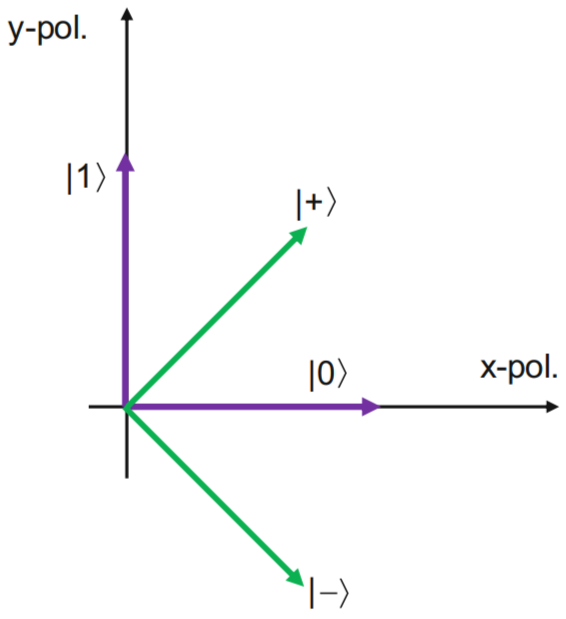
\includegraphics[width=0.4\textwidth]{chapters/figs/fig-7-4}
	\caption{چهار حالت به‌کار رفته در پروتکل \lr{BB84}.}
	\label{fig:7-4}
\end{figure}

\begin{figure}[ht]
	\centering
	 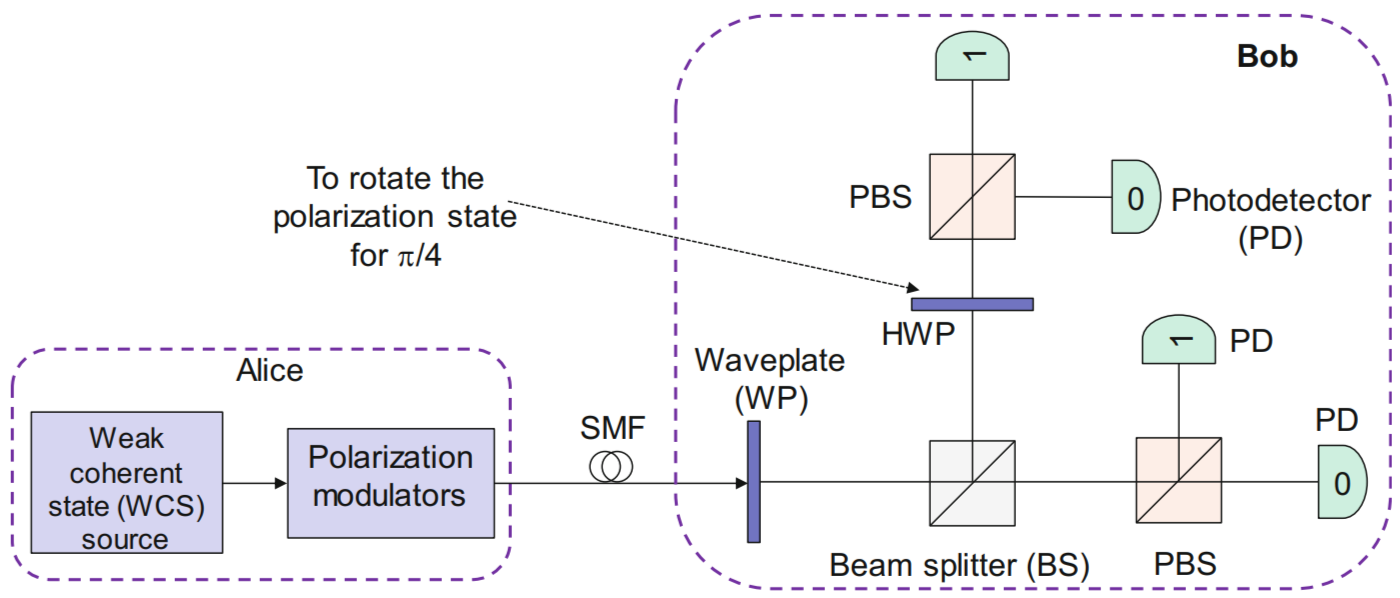
\includegraphics[width=0.9\textwidth]{chapters/figs/fig-7-5}
	\caption{پروتکل \lr{BB84} مبتنی بر قطبش.}
	\label{fig:7-5}
\end{figure}

حالت خروجی لیزر به‌عنوان حالت همدوس\LTRfootnote{Coherent state} شناخته می‌شود \cite{7-29, 7-30, 7-31, 7-32, 7-33, 7-34} که نشان‌دهنده کِت ویژه\LTRfootnote{Eigenket} راستِ عملگر نابودی\LTRfootnote{Annihilation operator} $a$ است؛ یعنی $a|\alpha\rangle = \alpha|\alpha\rangle$ که در آن $\alpha$ یک مقدار ویژه\LTRfootnote{Eigenvalue} مختلط است. بردار حالت همدوس $|\alpha\rangle$ را می‌توان برحسب کِت‌های ویژه متعامد پیش‌هنجار\LTRfootnote{Orthonormal eigenkets} $|n\rangle$ (حالت تعداد\LTRfootnote{Number state} یا حالت فوک\LTRfootnote{Fock state}) از عملگر تعداد\LTRfootnote{Number operator} $\hat{N} = a^\dagger a$ به‌صورت زیر نمایش داد:
\begin{equation}
	|\alpha\rangle = \exp[-|\alpha|^2/2] \sum_{n=0}^{+\infty} (n!)^{-1/2} \alpha^n |n\rangle
	\label{eq:7-10}
\end{equation}
حالت‌های همدوس متعامد نیستند، زیرا رابطه زیر برقرار است:







\begin{equation}
	\begin{aligned}
		|\langle\alpha | \beta\rangle|^2 &= \left| e^{-(|\alpha|^2+|\beta|^2)/2} \sum_{n=0}^{+\infty} \sum_{m=0}^{+\infty} (n!)^{-1/2}(m!)^{-1/2} \alpha^n (\beta^*)^m \langle n|m\rangle \right|^2 \\
		&= \left| e^{-(|\alpha|^2+|\beta|^2)/2} \sum_{n=0}^{+\infty} (n!)^{-1} \alpha^n (\beta^*)^n \right|^2 \\
		&= \left| e^{-(|\alpha|^2+|\beta|^2-2\alpha\beta^*)/2} \right|^2 = e^{-|\alpha-\beta|^2}.
	\end{aligned}
	\label{eq:7-11}
\end{equation}
زمانی که حالت همدوس به‌قدر کافی تضعیف شود، به حالت همدوس ضعیف\LTRfootnote{Weak coherent state} تبدیل می‌شود که می‌تواند تضمین کند حالت همدوس با احتمال بالایی بیش از یک فوتون نداشته باشد. به‌عنوان مثال، برای $0.1 = \alpha$ خواهیم داشت: $\dots + |2\rangle \sqrt{0.002} + |1\rangle \sqrt{0.09} + |0\rangle \sqrt{0.90} = |0.1\rangle$. حالت تعداد\LTRfootnote{Number state} $|n\rangle$ را می‌توان برحسب حالت پایه\LTRfootnote{Ground state} ($|0\rangle$) و با کمک عملگر تولید\LTRfootnote{Creation operator} به‌صورت زیر بیان کرد:
\begin{equation}
	|n\rangle = \frac{(a^\dagger)^n |0\rangle}{(n!)^{1/2}}.
	\label{eq:7-12}
\end{equation}
عملگر چگالی\LTRfootnote{Density operator} یک حالت همدوس به‌صورت زیر داده می‌شود:
\begin{equation}
	\rho = |\alpha\rangle\langle\alpha| = e^{-|\alpha|^2} \sum_{n=0}^{+\infty} \sum_{m=0}^{+\infty} (n!)^{-1/2}(m!)^{-1/2} \alpha^n (\alpha^*)^m |n\rangle\langle m|.
	\label{eq:7-13}
\end{equation}
جملات قطری $\rho$ به‌صورت زیر تعیین می‌شوند:
\begin{equation}
	\langle n | \rho | n \rangle = e^{-|\alpha|^2} \frac{|\alpha|^{2n}}{n!},
	\label{eq:7-14}
\end{equation}
که آشکارا یک توزیع پواسون\LTRfootnote{Poisson distribution} برای میانگین تعداد فوتون‌های $|\alpha|^2$ است. بنابراین، احتمال اینکه $n$ فوتون در حالت همدوس $|\alpha\rangle$ یافت شود، از توزیع پواسون پیروی می‌کند:
\begin{equation}
	P(n) = |\langle n | \alpha \rangle|^2 = e^{-\mu} \frac{\mu^n}{n!},
	\label{eq:7-15}
\end{equation}
که در آن از $\mu = |\alpha|^2$ برای نشان دادن میانگین تعداد فوتون‌ها استفاده شده است. با توجه به اینکه اکنون احتمال ارسال چندین فوتون غیرصفر است، ایو می‌تواند از این واقعیت برای کسب اطلاعات از کانال بهره‌برداری کند که با عنوان حمله تقسیم تعداد فوتون\LTRfootnote{Photon number splitting (PNS) attack} (\lr{PNS}) شناخته می‌شود. با فرض اینکه ایو قادر به تشخیص تعداد فوتون‌های رسیده به خود بدون انجام اندازه‌گیری روی سیستم باشد، زمانی که چندین فوتون شناسایی شوند، او یک تک‌فوتون را برداشته و آن را در حافظه کوانتومی\LTRfootnote{Quantum memory} قرار می‌دهد تا زمانی که آلیس و باب غربال‌گری زمانی و مصالحه پایه‌ها\LTRfootnote{Basis reconciliation} را انجام دهند. با یادگیری پایه‌های اندازه‌گیری آلیس و باب از طریق بحث در کانال عمومی احرازهویت‌شده، فوتون ذخیره‌شده در حافظه کوانتومی در پایه صحیح اندازه‌گیری شده و تمام اطلاعات موجود در فوتون در اختیار ایو قرار می‌گیرد.

برای غلبه بر حمله \lr{PNS}، استفاده از توزیع کلید کوانتومی مبتنی بر حالت فریب\LTRfootnote{Decoy state} در مرجع \cite{7-35} پیشنهاد شد. در \lr{QKD} حالت فریب، میانگین تعداد فوتون‌های ارسالی در بازه‌های زمانی تصادفی افزایش می‌یابد که به آلیس و باب اجازه می‌دهد تشخیص دهند آیا در زمان ارسال چندین فوتون، ایو در حال سرقت فوتون‌ها است یا خیر.











\subsubsection{\lr{QKD} \lr{BB84} مبتنی بر کدگذاری فاز}
\label{subsec:7-3-1-4}
اکنون پروتکل \lr{QKD} \lr{BB84} مبتنی بر کدگذاری فاز\LTRfootnote{Phase encoding} را شرح می‌دهیم که نسخه اپتیک حجیم\LTRfootnote{Bulky optics} آن در شکل \ref{fig:7-6} تصویر شده است.

\begin{figure}[ht]
	\centering
	 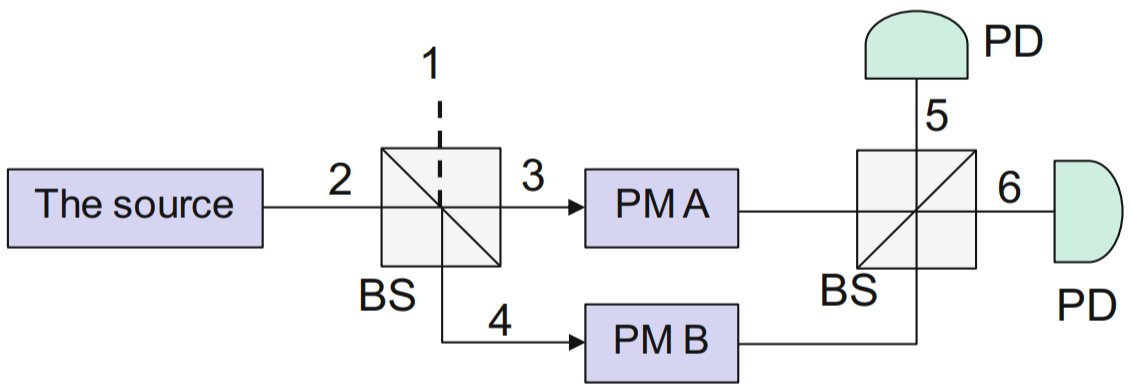
\includegraphics[width=0.8\textwidth]{chapters/figs/fig-7-6}
	\caption{پروتکل \lr{BB84} مبتنی بر کدگذاری فاز.}
	\label{fig:7-6}
\end{figure}

حالت پایه فوک\LTRfootnote{Fock basis} دو-مُدی ورودی $|01\rangle_{n_1 n_2}$ پس از اولین تقسیم‌کننده پرتو\LTRfootnote{Beam splitter} (\lr{BS}) به صورت زیر تبدیل می‌شود:
\begin{equation}
	|01\rangle_{n_1 n_2} \rightarrow 2^{-1/2}(j|01\rangle_{n_3 n_4} + |10\rangle_{n_3 n_4})
	\label{eq:7-16}
\end{equation}
پس از اعمال جابه‌جایی‌های فاز در شاخه‌های ماخ-زندر\LTRfootnote{Mach-Zehnder (MZ)} (\lr{MZ})، می‌توانیم بنویسیم:
\begin{equation}
	2^{-1/2}(j|01\rangle_{n_3 n_4} + |10\rangle_{n_3 n_4}) \rightarrow 2^{-1/2}(je^{-j\phi/2}|01\rangle_{n_3 n_4} + e^{j\phi/2}|10\rangle_{n_3 n_4}), \quad \phi = \phi_A - \phi_B
	\label{eq:7-17}
\end{equation}
که در آن $\phi_A$ ($\phi_B$) متناظر با جابه‌جایی فاز اعمال شده در شاخه بالایی (پایینی) متعلق به آلیس (باب) است. پس از \lr{BS} دوم، حالت متناظر به‌صورت زیر خواهد بود:
\begin{equation}
	|01\rangle_{n_3 n_4} \rightarrow 2^{-1/2}(j|01\rangle_{n_5 n_6} + |10\rangle_{n_5 n_6}), \quad |10\rangle_{n_3 n_4} \rightarrow 2^{-1/2}(j|10\rangle_{n_5 n_6} + |01\rangle_{n_5 n_6})
	\label{eq:7-18}
\end{equation}
حالت خروجی کلی را می‌توان به‌صورت زیر نمایش داد:
\begin{equation}
	|\psi(\phi)\rangle = j(\sin(\phi/2)|01\rangle_{n_5 n_6} + \cos(\phi/2)|10\rangle_{n_5 n_6})
	\label{eq:7-19}
\end{equation}
با تنظیم فازهای $\phi$ مختلف، می‌توانیم حالت‌های پروتکل \lr{BB84} را به‌صورت زیر تعریف کنیم:
\begin{equation}
	\begin{aligned}
		|\psi(0)\rangle &= j|10\rangle_{n_5 n_6} \doteq |0\rangle, \quad |\psi(\pi)\rangle = j|01\rangle_{n_5 n_6} \doteq |1\rangle \\
		|\psi(\pi/2)\rangle &= j2^{-1/2}(|10\rangle_{n_5 n_6} + |01\rangle_{n_5 n_6}) \doteq |+\rangle, \\
		|\psi(-\pi/2)\rangle &= j2^{-1/2}(|10\rangle_{n_5 n_6} - |01\rangle_{n_5 n_6}) \doteq |-\rangle
	\end{aligned}
	\label{eq:7-20}
\end{equation}
آلیس به‌طور تصادفی ولتاژ کنترل را برای اعمال جابه‌جایی فاز $\phi_A \in \{-\pi/2, 0, \pi/2, \pi\}$ تنظیم کرده و بنابراین به‌طور تصادفی حالت را انتخاب می‌کند. باب پایه اندازه‌گیری را با انتخاب تصادفی $\phi_B \in \{0, \pi/2\}$ برمی‌گزیند. اندازه‌گیری قاطع\LTRfootnote{Conclusive measurement} زمانی رخ می‌دهد که یا: (۱) $\phi_B = 0$ و $\phi_A \in \{0, \pi\}$ باشد و یا (۲) $\phi_B = \pi/2$ و $\phi_A \in \{-\pi/2, \pi/2\}$ باشد.













\subsection{پروتکل B92}
\label{subsec:7-3-2}
پروتکل \lr{B92} که در سال ۱۹۹۲ توسط بنت معرفی شد \cite{7-36}، تنها از دو حالت غیرمتعامد استفاده می‌کند، همان‌طور که در شکل \ref{fig:7-7} تصویر شده است. آلیس به‌طور تصادفی یک بیت کلاسیک $d$ تولید می‌کند و بسته به مقدار آن (۰ یا ۱)، حالت زیر را برای باب ارسال می‌نماید \cite{7-6}:
\begin{equation}
	|\psi\rangle = \begin{cases} 
		|0\rangle, & d = 0 \\ 
		|+\rangle = (|0\rangle + |1\rangle)/\sqrt{2}, & d = 1 
	\end{cases}
	\label{eq:7-21}
\end{equation}

\begin{figure}[ht]
	\centering
	% \includegraphics[width=0.6\textwidth]{fig7-7}
	\caption{دو حالت به‌کار رفته در پروتکل \lr{B92}.}
	\label{fig:7-7}
\end{figure}

باب به‌طور تصادفی یک بیت کلاسیک $d'$ تولید کرده و متعاقباً کیوبیت‌های دریافتی را در پایه محاسباتی\LTRfootnote{Computational basis} $CB = \{|0\rangle, |1\rangle\}$ (اگر $d'=0$) یا پایه قطری\LTRfootnote{Diagonal basis} $DB = \{|+\rangle, |-\rangle\}$ (اگر $d'=1$) اندازه‌گیری می‌کند؛ به‌طوری که نتیجه اندازه‌گیری $r=0$ یا ۱، متناظر با حالت‌های ویژه\LTRfootnote{Eigenstates} $1-$ و $1+$ از مشاهده‌پذیرهای\LTRfootnote{Observables} $X$ و $Z$ است که در جدول \ref{tab:7-1} نشان داده شده است. به‌وضوح، زمانی که نتیجه اندازه‌گیری $r=0$ باشد، حالت‌های احتمالی ارسال شده توسط آلیس $|0\rangle$ و $|+\rangle$ هستند و باب نمی‌داند آلیس کدام حالت را ارسال کرده است. از سوی دیگر، هنگامی که نتیجه اندازه‌گیری $r=1$ باشد، حالت‌های احتمالی آشکار شده توسط باب $|1\rangle$ و $|-\rangle$ هستند و بیت آشکار شده توسط باب متمم\LTRfootnote{Complement} بیت آلیس است.





\begin{table}[ht]
	\centering
	\caption{توضیح پروتکل \lr{B92}.}
	\label{tab:7-1}
	
	\small
	\begin{tabular}{|l|c|c|c|c|}
		\hline
		بیت‌های تولید شده توسط آلیس & \multicolumn{2}{c|}{$d = 0$} & \multicolumn{2}{c|}{$d = 1$} \\ \hline
		حالت‌های ارسال شده توسط آلیس & \multicolumn{2}{c|}{$|0\rangle$} & \multicolumn{2}{c|}{$|+\rangle$} \\ \hline
		بیت‌های تولید شده توسط باب & $d' = 0$ & $d' = 1$ & $d' = 0$ & $d' = 1$ \\ \hline
		پایه اندازه‌گیری باب & \lr{CB}: $\{|0\rangle, |1\rangle\}$ & \lr{DB}: $\{|+\rangle, |-\rangle\}$ & \lr{CB}: $\{|0\rangle, |1\rangle\}$ & \lr{DB}: $\{|+\rangle, |-\rangle\}$ \\ \hline
		\begin{tabular}[c]{@{}l@{}}حالت‌های حاصل احتمالی برای\\ آشکارسازی توسط باب\end{tabular} & $|0\rangle \quad |1\rangle$ & $|+\rangle \quad |-\rangle$ & $|0\rangle \quad |1\rangle$ & $|+\rangle \quad |-\rangle$ \\ \hline
		\begin{tabular}[c]{@{}l@{}}احتمال اندازه‌گیری یک\\ حالت معین توسط باب\end{tabular} & $1 \quad 0$ & $1/2 \quad 1/2$ & $1/2 \quad 1/2$ & $1 \quad 0$ \\ \hline
		نتیجه اندازه‌گیری باب $r$ & $0 \quad -$ & $0 \quad 1$ & $0 \quad 1$ & $0 \quad -$ \\ \hline
	\end{tabular}
\end{table}






باب به‌صورت عمومی مقدار $r$ را اعلام می‌کند (و البته $d'$ را مخفی نگه می‌دارد). آلیس و باب تنها آن جفت‌های $\{d, d'\}$ را نگه می‌دارند که برای آن‌ها نتیجه اندازه‌گیری $r=1$ بوده است. بیت نهایی کلید برای آلیس $d$ و برای باب $1-d'$ است. سپس مراحل مصالحه اطلاعات و تقویت حریم خصوصی انجام می‌شوند.








\subsection{پروتکل‌های اکرت (E91) و EPR}
\label{subsec:7-3-3}
پروتکل اکرت (\lr{E91})\LTRfootnote{Ekert (E91) protocol} در سال ۱۹۹۱ توسط اکرت معرفی شد \cite{7-37} (همچنین ببینید \cite{7-6}). فرض کنید آلیس و باب $n$ جفت‌کیوبیت درهم‌تنیده\LTRfootnote{Entangled} در حالت بل\LTRfootnote{Bell state} (جفت \lr{EPR}) $|B_{00}\rangle$ را به اشتراک می‌گذارند:
\begin{equation}
	|B_{00}\rangle = \frac{|00\rangle + |11\rangle}{\sqrt{2}}
	\label{eq:7-22}
\end{equation}
آلیس یک بیت کلاسیک تصادفی $b$ را برای تعیین پایه تولید کرده و نیمه خود از حالت بل را یا در پایه محاسباتی\LTRfootnote{Computational basis} $CB = \{|0\rangle, |1\rangle\}$ برای $b=0$ یا در پایه قطری\LTRfootnote{Diagonal basis} $DB = \{|+\rangle, |-\rangle\}$ برای $b=1$ اندازه‌گیری می‌کند تا بیت داده $d$ را به‌دست آورد. از سوی دیگر، باب به شیوه‌ای مشابه، به‌طور تصادفی بیت پایه $b'$ را تولید کرده و اندازه‌گیری را در یکی از پایه‌های \lr{CB} یا \lr{DB} انجام می‌دهد تا $d'$ را به‌دست آورد. آلیس و باب پایه‌های استفاده شده، یعنی $b$ و $b'$ را با هم مقایسه می‌کنند و تنها آن مواردی از $\{d, d'\}$ را برای کلید خام خود نگه می‌دارند که در آن‌ها پایه‌ها یکسان بوده است ($b=b'$). واضح است که کلید خام تولید شده به‌این صورت، کاملاً تصادفی است و تا زمانی که آلیس و باب اندازه‌گیری را روی نیمه‌های خود از حالت بل انجام ندهند، نامعین باقی می‌ماند. به همین دلیل، \lr{QKD} اساساً یک روش تولید کلید مخفی است، زیرا توسط منبع درهم‌تنیده تعیین می‌شود. اگر به جای آن، از حالت بل $|B_{01}\rangle = (|01\rangle + |10\rangle)/\sqrt{2}$ استفاده می‌شد، دنباله کلید خام باب متمم دنباله کلید خام آلیس می‌بود.

پروتکل \lr{EPR} یک پروتکل سه‌حالتی است که از نامساوی بل\LTRfootnote{Bell's inequality} برای تشخیص حضور ایو به‌عنوان یک متغیر تصادفی پنهان\LTRfootnote{Hidden random variable} استفاده می‌کند، همان‌طور که در مرجع \cite{7-38} توصیف شده است. فرض کنید $|\theta\rangle$ نشان‌دهنده حالت قطبش فوتونی باشد که به‌صورت خطی در زاویه $\theta$ قطبیده شده است. سه حالت قطبش ممکن برای جفت \lr{EPR} عبارتند از \cite{7-38}:
\begin{equation}
	\begin{aligned}
		|B_0\rangle &= \frac{|0\rangle|3\pi/6\rangle + |3\pi/6\rangle|0\rangle}{\sqrt{2}}, \\
		|B_1\rangle &= \frac{|\pi/6\rangle|4\pi/6\rangle + |4\pi/6\rangle|\pi/6\rangle}{\sqrt{2}}, \\
		|B_2\rangle &= \frac{|2\pi/6\rangle|5\pi/6\rangle + |5\pi/6\rangle|2\pi/6\rangle}{\sqrt{2}}
	\end{aligned}
	\label{eq:7-23}
\end{equation}
برای هر یک از این جفت‌های \lr{EPR}، قواعد کدگذاری زیر را اعمال می‌کنیم \cite{7-38}:
\begin{equation}
	|\psi\rangle_1 = \begin{cases} |0\rangle, & d=0 \\ |3\pi/6\rangle, & d=1 \end{cases}; \quad 
	|\psi\rangle_2 = \begin{cases} |\pi/6\rangle, & d=0 \\ |4\pi/6\rangle, & d=1 \end{cases}; \quad 
	|\psi\rangle_3 = \begin{cases} |2\pi/6\rangle, & d=0 \\ |5\pi/6\rangle, & d=1 \end{cases}
	\label{eq:7-24}
\end{equation}
عملگرهای اندازه‌گیری\LTRfootnote{Measurement operators} متناظر به‌صورت زیر خواهند بود \cite{7-38}:
\begin{equation}
	M_0 = |0\rangle\langle 0|, \quad M_1 = |\pi/6\rangle\langle \pi/6|, \quad M_2 = |2\pi/6\rangle\langle 2\pi/6|
	\label{eq:7-25}
\end{equation}
پروتکل \lr{EPR} را می‌توان اکنون به شرح زیر توصیف کرد. حالت \lr{EPR} یعنی $|B_i\rangle$ ($i=0,1,2$) به‌طور تصادفی انتخاب می‌شود. فوتون اول در جفت \lr{EPR} برای آلیس و فوتون دوم برای باب ارسال می‌شود. آلیس و باب به‌طور تصادفی، مستقل و با احتمال یکسان، یکی از عملگرهای اندازه‌گیری $M_0$، $M_1$ و $M_2$ را انتخاب می‌کنند. آن‌ها متعاقباً فوتون (کیوبیت) مربوط به خود را اندازه‌گیری می‌کنند و نتایج اندازه‌گیری، بیت متناظر برای کلید غربال‌شده\LTRfootnote{Sifted key} را تعیین می‌کند. به‌وضوح، انتخاب جفت‌های \lr{EPR} مطابق با رابطه \eqref{eq:7-23} منجر به کلیدهای خام متمم می‌شود. آلیس و باب سپس از طریق یک کانال عمومی احرازهویت‌شده با یکدیگر ارتباط برقرار می‌کنند تا مواردی را که در آن‌ها از عملگر اندازه‌گیری یکسانی استفاده کرده‌اند تعیین کنند و آن موارد را نگه می‌دارند. کلید مشترک حاصل، نشان‌دهنده کلید غربال‌شده است. مواردی که در آن‌ها از عملگرهای اندازه‌گیری متفاوتی استفاده کرده‌اند، نشان‌دهنده کلید ردشده\LTRfootnote{Rejected key} است و از این موارد برای تشخیص حضور ایو با به‌کارگیری نامساوی بل روی کلید ردشده استفاده می‌شود. آلیس و باب سپس مراحل مصالحه اطلاعات و تقویت حریم خصوصی را انجام می‌دهند.

اکنون به شرح این موضوع می‌پردازیم که چگونه کلید ردشده می‌تواند برای تشخیص حضور ایو مورد استفاده قرار گیرد \cite{7-38}. فرض کنید $P(\neq|i,j)$ نشان‌دهنده احتمال متفاوت بودن بیت‌های آلیس و باب در کلید ردشده باشد، با این فرض که عملگرهای اندازه‌گیری آلیس و باب به‌ترتیب یا $M_i$ و $M_j$ و یا $M_j$ و $M_i$ باشند. علاوه بر این، فرض کنید $P(=|i,j) = 1 - P(\neq|i,j)$ باشد. تفاضل بین این دو احتمال را با $\Delta P(i,j) = P(\neq|i,j) - P(=|i,j)$ نشان می‌دهیم. پارامتر بل\LTRfootnote{Bell's parameter} را می‌توان به‌صورت زیر تعریف کرد \cite{7-38}:
\begin{equation}
	\beta = 1 + \Delta P(1,2) - |\Delta P(0,1) - \Delta P(0,2)|
	\label{eq:7-26}
\end{equation}
که برای عملگرهای اندازه‌گیری فوق به $\beta \geq 0$ کاهش می‌یابد. با این حال، پیش‌بینی مکانیک کوانتومی مقدار $\beta = -1/2$ را به‌دست می‌دهد که به‌وضوح ناقض نامساوی بل است.












\subsection{کدگذاری فاز-زمان}
\label{subsec:7-3-4}
پروتکل \lr{BB84} علاوه بر حالت‌های قطبش، با استفاده از درجات آزادی\LTRfootnote{Degrees of freedom (DOF)} مختلفی مانند کدگذاری فاز-زمان\LTRfootnote{Time-phase encoding} \cite{7-39, 7-40, 7-41} و تکانه زاویه‌ای مداری\LTRfootnote{Orbital angular momentum} \cite{7-42, 7-43} نیز قابل پیاده‌سازی است. حالت‌های کدگذاری فاز-زمان برای پروتکل \lr{BB84} در شکل \ref{fig:7-8} ارائه شده‌اند که در مقایسه با شکل \ref{fig:7-6}، نسخه متفاوتی از طرح کدگذاری فاز محسوب می‌شود.

\begin{figure}[ht]
	\centering
	 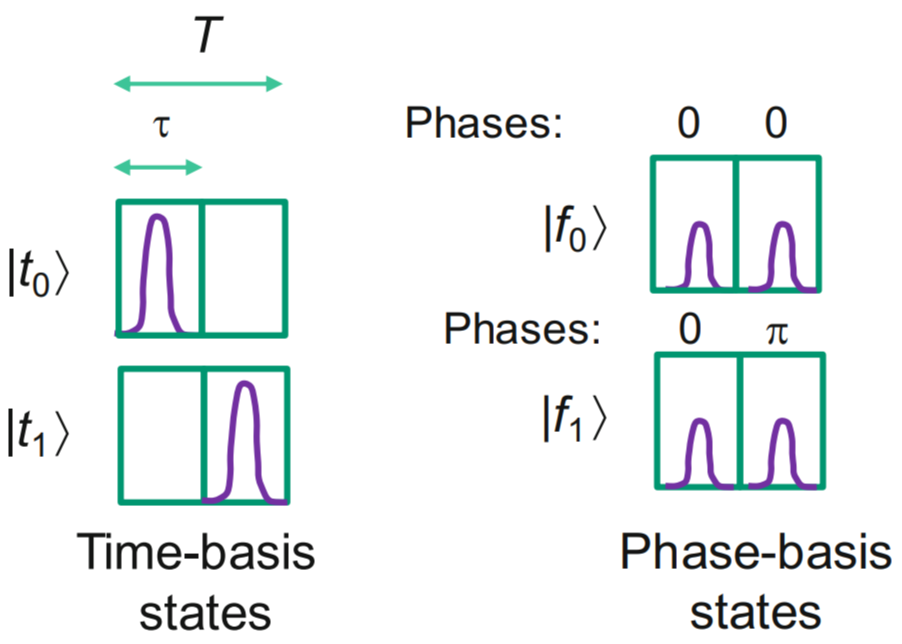
\includegraphics[width=0.7\textwidth]{chapters/figs/fig-7-8}
	\caption{حالت‌های کدگذاری فاز-زمان مورد استفاده در پروتکل \lr{BB84}.}
	\label{fig:7-8}
\end{figure}

پایه زمانی\LTRfootnote{Time basis} متناظر با پایه محاسباتی\LTRfootnote{Computational basis} و پایه فازی\LTRfootnote{Phase basis} متناظر با پایه قطری\LTRfootnote{Diagonal basis} است. پالس در یک بازه زمانی\LTRfootnote{Time bin} با مدت‌زمان $\tau = T/2$ متمرکز شده است. پایه زمانی مشابه مدولاسیون موقعیت پالس\LTRfootnote{Pulse-position modulation (PPM)} (\lr{PPM}) است. حالتی که در آن فوتون در اولین بازه زمانی قرار می‌گیرد با $|t_0\rangle$ و حالتی که در آن فوتون در دومین بازه زمانی قرار می‌گیرد با $|t_1\rangle$ نشان داده می‌شود. حالت‌های پایه‌های متقابلاً بدون سوگیری\LTRfootnote{Mutually unbiased bases (MUBs)} (\lr{MUB}) فازی به‌صورت زیر تعریف می‌شوند:
\begin{equation}
	|f_0\rangle = \frac{1}{\sqrt{2}} (|t_0\rangle + |t_1\rangle), \quad |f_1\rangle = \frac{1}{\sqrt{2}} (|t_0\rangle - |t_1\rangle).
	\label{eq:7-27}
\end{equation}

آلیس به‌طور تصادفی یا پایه زمانی و یا پایه فازی را انتخاب کرده و سپس به‌طور تصادفی یکی از حالت‌های پایه را برمی‌گزیند. مقدار منطقی $0$ توسط $|t_0\rangle$ و $|f_0\rangle$ و مقدار منطقی $1$ توسط $|t_1\rangle$ و $|f_1\rangle$ بازنمایی می‌شود. باب هر کیوبیت را با انتخاب تصادفی پایه، یعنی پایه زمانی یا فازی، اندازه‌گیری می‌کند. در فرآیند غربال‌گری\LTRfootnote{Sifting procedure}، آلیس و باب پایه‌های استفاده شده برای هر کیوبیت را اعلام کرده و تنها مواردی را که از پایه یکسانی استفاده کرده‌اند، نگه می‌دارند.

برای پیاده‌سازی رمزگذار فاز-زمان، می‌توان از مدولاتور قطبی الکترواپتیکی\LTRfootnote{Electro-optical polar modulator} (متشکل از اتصال پیاپی یک مدولاتور دامنه\LTRfootnote{Amplitude modulator} و یک مدولاتور فاز\LTRfootnote{Phase modulator}) یا مدولاتور \lr{I/Q} استفاده کرد \cite{7-44}. مدولاتور دامنه (مدولاتور ماخ-زندر\LTRfootnote{Mach-Zehnder modulator}) برای شکل‌دهی پالس و مدولاتور فاز برای اعمال جابه‌جایی فاز مطلوب به کار می‌روند، همان‌طور که در شکل \ref{fig:7-9} نشان داده شده است. از مولد شکل‌موج دلخواه\LTRfootnote{Arbitrary waveform generator (AWG)} (\lr{AWG}) برای تولید شکل‌موج‌های \lr{RF} متناظر بر حسب نیاز استفاده می‌شود. تضعیف‌کننده نوری متغیر\LTRfootnote{Variable optical attenuator (VOA)} (\lr{VOA}) نیز برای تضعیف باریکه مدوله‌شده تا سطح تک‌فوتون به کار می‌رود.



\begin{figure}[ht]
	\centering
	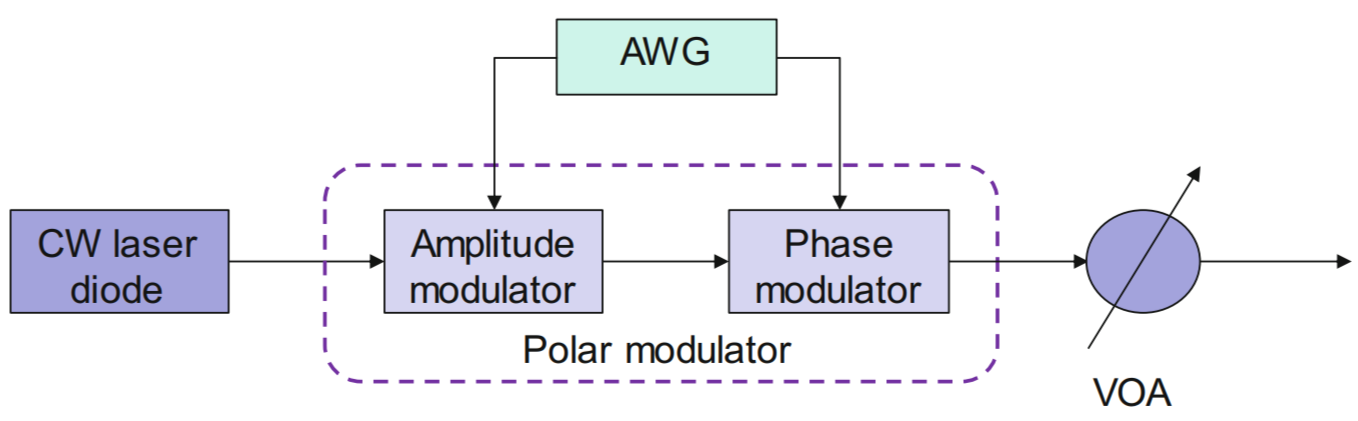
\includegraphics[width=0.8\textwidth]{chapters/figs/fig-7-9}
	\caption{رمزگذار فاز-زمان برای پروتکل \lr{QKD} \lr{BB84}. \lr{AWG}: مولد شکل‌موج دلخواه؛ \lr{VOA}: تضعیف‌کننده نوری متغیر.}
	\label{fig:7-9}
\end{figure}

در سمت گیرنده، حالت‌های پایه زمانی را می‌توان با کمک یک شمارنده تک‌فوتون\LTRfootnote{Single-photon counter} و مدارهای الکترونیکی مناسب آشکارسازی کرد. از سوی دیگر، برای آشکارسازی حالت‌های پایه فازی، می‌توان از یک تداخل‌سنج تأخیر-زمانی\LTRfootnote{Time-delay interferometer} استفاده کرد، همان‌طور که در مرجع \cite{7-45} توصیف شده است (شکل \ref{fig:7-10} را ببینید). اختلاف مسیر بین دو بازو برابر است با $\Delta L = \Delta L_0 + \delta L$ \cite{7-45}، که در آن $\Delta L_0$ اختلاف مسیری برابر با $c\tau$ ($c$ سرعت نور است) و $\delta L \ll \Delta L_0$ اختلاف مسیر اندکی است که برای تنظیم فاز استفاده می‌شود، زیرا $\phi = k\delta L$ ($k$ عدد موج\LTRfootnote{Wave number} است). هنگامی که حالت فازی $|f_0\rangle$ به رمزگشای فاز-زمان وارد می‌شود، خروجی‌های دومین تقسیم‌کننده پرتو\LTRfootnote{Beam splitter (BS)} (\lr{BS}) ۵۰:۵۰ سه بازه زمانی را اشغال می‌کنند. خروجی $+$ موردی را نشان می‌دهد که در آن خروجی‌های تداخل‌سنج تداخل سازنده\LTRfootnote{Constructive interference} دارند، در حالی که خروجی $-$ نشان‌دهنده تداخل ویرانگر\LTRfootnote{Destructive interference} خروجی‌های متناظر تداخل‌سنج است. برای تداخل سازنده، پالس میانی دوبرابر می‌شود، در حالی که برای تداخل ویرانگر، پالس‌های میانی یکدیگر را خنثی می‌کنند. بنابراین، کلیک آشکارساز تک‌فوتون\LTRfootnote{Single-photon detector (SPD)} (\lr{SPD}) در بازه میانی در خروجی $+$، حالت $|f_0\rangle$ را شناسایی می‌کند، در حالی که کلیک متناظر در خروجی $-$، حالت $|f_1\rangle$ را تشخیص می‌دهد.



\begin{figure}[ht]
	\centering
	 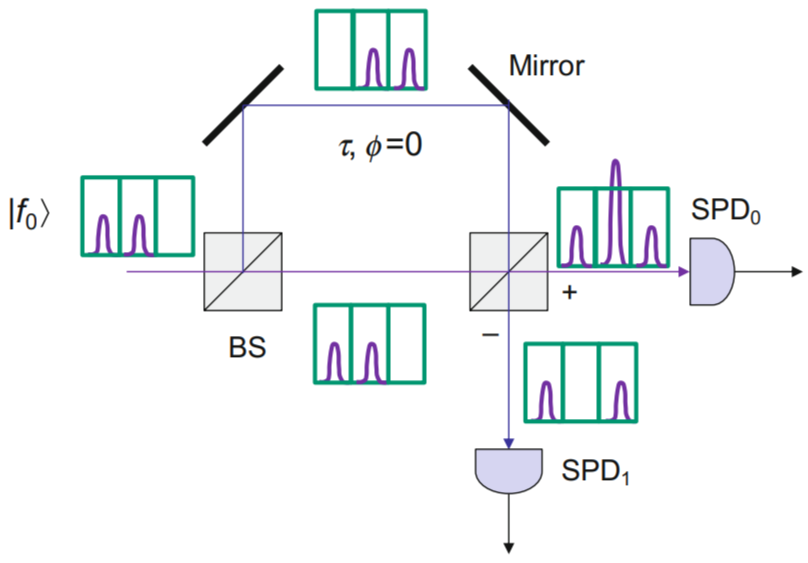
\includegraphics[width=0.8\textwidth]{chapters/figs/fig-7-10}
	\caption{رمزگشای فاز-زمان برای پروتکل \lr{QKD} \lr{BB84}. \lr{BS}: تقسیم‌کننده پرتو ۵۰:۵۰؛ \lr{SPD}: آشکارساز تک‌فوتون.}
	\label{fig:7-10}
\end{figure}







\section{مسائل امنیتی سیستم‌های \lr{QKD}}
\label{sec:7-4}
همان‌طور که در مرور کلی پروتکل \lr{BB84} بحث شد، پس از اتمام مرحله ارسال کلید خام، آلیس و باب فرآیند غربال‌گری\LTRfootnote{Sifting procedure} و تخمین پارامتر\LTRfootnote{Parameter estimation} را انجام می‌دهند، به‌طوری که از $N$ نماد ارسال شده، $n$ نماد باقی می‌ماند و کلید متناظر با آن‌ها، کلید غربال‌شده\LTRfootnote{Sifted key} نامیده می‌شود. سپس، آن‌ها پس‌پردازش کلاسیک مانند مصالحه اطلاعات\LTRfootnote{Information reconciliation} و تقویت حریم خصوصی\LTRfootnote{Privacy amplification} را انجام می‌دهند. در مرحله مصالحه اطلاعات، آن‌ها از تصحیح خطا برای اصلاح خطاهای ایجاد شده توسط هر دو عاملِ کانال کوانتومی و ایو استفاده می‌کنند؛ کلید متناظر پس از اتمام این مرحله معمولاً کلید اصلاح‌شده\LTRfootnote{Corrected key} نامیده می‌شود. در طول تقویت حریم خصوصی، آن‌ها همبستگی باقی‌مانده با ایو را حذف می‌کنند و از $n$ نماد، $m$ نماد باقی می‌ماند که کلید متناظر، کلید امن\LTRfootnote{Secure key} است. به‌وضوح، نرخ کسرِ کلید مخفی $r$ را می‌توان به‌صورت $r = m/n$ (در حالت $N \to \infty$) تعیین کرد که اغلب به آن کسر مخفی\LTRfootnote{Secret fraction} گفته می‌شود \cite{7-46}. نرخ کلید مخفی (\lr{SKR})\LTRfootnote{Secret-key rate (SKR)} سپس به‌صورت حاصل‌ضرب کسر مخفی و نرخ کلید خام، که با $R_{\text{raw}}$ نشان داده می‌شود، تعیین می‌گردد و می‌توانیم بنویسیم \cite{7-46}:
\begin{equation}
	\text{SKR} = r \cdot R_{\text{raw}}
	\label{eq:7-28}
\end{equation}
جالب اینجاست که در بسیاری از مقالات، اصطلاح \lr{SKR} به همان کسر مخفی $r$ اشاره دارد. با توجه به اینکه نرخ کلید خام توسط دستگاه‌های مورد استفاده (به‌ویژه آشکارساز تک‌فوتون\LTRfootnote{Single-photon detector (SPD)} (\lr{SPD})) و کانال کوانتومی که ارسال در آن صورت می‌گیرد تعیین می‌شود و نه توسط قوانین فیزیک کوانتوم، نرخ کسری را می‌توان نرخ \lr{SKR} نرمالیزه‌شده نیز نامید، چرا که $r = \text{SKR}/R_{\text{raw}}$.

نرخ کلید خام را می‌توان به‌صورت حاصل‌ضرب نرخ سیگنال‌دهی $R_s$ و احتمال پذیرش نماد ارسالی توسط باب به‌طور میانگین، که با $\text{Pr}(\text{\lr{Bob accepting}})$ نشان داده می‌شود، تعیین کرد؛ بنابراین می‌توانیم بنویسیم:
\begin{equation}
	R_{\text{raw}} = R_s \cdot \text{Pr}(\text{\lr{Bob accepting}})
	\label{eq:7-29}
\end{equation}
از سوی دیگر، نرخ سیگنال‌دهی توسط رابطه زیر تعیین می‌شود \cite{7-46}:
\begin{equation}
	R_s = \min \left( R_{s, \text{max}} , 1/T_{dc}, \frac{\mu T T_B \eta}{\tau_{\text{dead}}} \right)
	\label{eq:7-30}
\end{equation}
که در آن $R_{s, \text{max}}$ حداکثر نرخ سیگنال‌دهی مجاز توسط منبع، $T_{dc}$ چرخه کاری\LTRfootnote{Duty cycle} و $\tau_{\text{dead}}$ زمان مرده\LTRfootnote{Dead time} مربوط به \lr{SPD} (زمان مورد نیاز برای بازنشانی \lr{SPD} پس از آشکارسازی یک فوتون) است. عبارت $\mu T T_B \eta$ متناظر با احتمال آشکارسازی باب است، که در آن $\mu$ میانگین تعداد فوتون‌های تولید شده توسط منبع، $\eta$ بازدهی \lr{SPD}، $T$ گذردهی\LTRfootnote{Transmissivity} کانال کوانتومی و $T_B$ نشان‌دهنده تلفات در گیرنده باب است. کانال کوانتومی معمولاً یا کانال فیبر نوری است و یا کانال نوری فضای آزاد. تضعیف در کانال فیبر نوری با $T = 10^{-\alpha L / 10}$ تعیین می‌شود که در آن $\alpha$ ضریب تضعیف برحسب $\text{dB/km}$ و $L$ مسافت ارسال برحسب $\text{km}$ است. ضریب تضعیف معمول در فیبر تک‌مُد استاندارد (\lr{SSMF})\LTRfootnote{Standard single-mode fiber (SSMF)} در طول موج $1550$ نانومتر، $0.2$ $\text{dB/km}$ است. در مورد پیوند نوری فضای آزاد (\lr{FSO})، اگر از اثرات تلاطم اتمسفری\LTRfootnote{Atmospheric turbulence} صرف‌نظر کنیم، برای یک پیوند خط دید\LTRfootnote{Line-of-sight} با مسافت ارسال $L$، می‌توانیم تلفات پیوند \lr{FSO} را طبق مرجع \cite{7-47} به‌صورت زیر تخمین بزنیم:
$T = [d_{Rx}/(d_{Tx} + DL)]^2 \cdot 10^{-\alpha L / 10}$، که در آن $d_{Tx}$ و $d_{Rx}$ نشان‌دهنده قطر دهانه تلسکوپ‌های فرستنده و گیرنده و $D$ واگرایی\LTRfootnote{Divergence} است. بنابراین، جمله اول نشان‌دهنده تلفات هندسی و جمله دوم تضعیف میانگین ناشی از پراکندگی\LTRfootnote{Scattering} است، که ضریب تضعیف پراکندگی در شرایط آسمان صاف در طول‌موج‌های $1520$ تا $1600$ نانومتر کمتر از $0.1$ $\text{dB/km}$ است.

در پروتکل \lr{BB84}، احتمالی که باب نماد ارسالی را می‌پذیرد با احتمال استفاده او از پایه یکسان مرتبط است که با $p_{\text{sift}}$ نشان داده می‌شود، به‌طوری که نرخ سیگنال‌دهی به‌صورت $R_s p_{\text{sift}}$ در می‌آید و نرخ کلید خام زمانی که آلیس $n$ فوتون برای باب ارسال می‌کند، طبق مرجع \cite{7-46} برابر خواهد بود با:
\begin{equation}
	R_{\text{raw}, n} = R_s p_{\text{sift}} p_{A, n} p_n
	\label{eq:7-31}
\end{equation}
که در آن $p_{A, n}$ احتمال این است که پالس ارسال شده توسط آلیس شامل $n$ فوتون باشد (بخش زیر را ببینید) و $p_n$ احتمال این است که ایو پالسی با $n$ فوتون برای باب ارسال کند. نرخ کلید خام کلِ نهایی برابر با $R_{\text{raw}} = \sum_n R_{\text{raw}, n}$ خواهد بود.

آنچه برای تعیین باقی می‌ماند، نرخ کسر است. \lr{QKD} می‌تواند به امنیت غیرمشروط\LTRfootnote{Unconditional security} دست یابد، به این معنی که امنیت آن را می‌توان بدون اعمال هیچ‌گونه محدودیتی بر توان محاسباتی یا استراتژی شنود ایو، تأیید کرد. کران‌های مربوط به نرخ کسر به مراحل پس‌پردازش کلاسیک بستگی دارند. رایج‌ترین روش، پس‌پردازش یک‌طرفه\LTRfootnote{One-way postprocessing} است که در آن یا آلیس و یا باب کلید مرجع را در اختیار دارند و اطلاعات کلاسیک را از طریق کانال عمومی برای طرف دیگر ارسال می‌کنند، در حالی که طرف مقابل بدون ارائه بازخورد، فرآیند خاصی را روی داده‌ها انجام می‌دهد. مشابه طرح‌های امنیت لایه فیزیکی (\lr{PLS}) که در فصل \ref{chap:4} توصیف شد، معمول‌ترین پردازش یک‌طرفه شامل دو مرحله است: مصالحه اطلاعات و تقویت حریم خصوصی. عبارت مربوط به کسر مخفی که از طریق پس‌پردازش یک‌طرفه به‌دست می‌آید، بسیار مشابه طرح‌های \lr{PLS} کلاسیک است \cite{7-46}:
\begin{equation}
	r = I(\bm{A}; \bm{B}) - \min_{\text{\lr{Eve's strategies}}} (I_{EA}, I_{EB})
	\label{eq:7-32}
\end{equation}
که در آن $I(\bm{A}; \bm{B})$ اطلاعات متقابل بین آلیس و باب است، در حالی که جمله دوم متناظر با اطلاعات ایو $I_E$ درباره کلید خام آلیس یا باب است، که در آن کمینه‌سازی روی تمام استراتژی‌های شنود ممکن انجام می‌شود. آلیس و باب تصمیم خواهند گرفت که از مصالحه مستقیم یا معکوس استفاده کنند تا بتوانند اطلاعات ایو را کمینه نمایند.

اکنون استراتژی‌های مختلف شنود را که ایو ممکن است به کار گیرد و اطلاعات ایو $I_E$ را تعیین می‌کنند، شرح می‌دهیم.









\subsection{استراتژی‌های شنود و کسرهای مخفی متناظر}
\label{sec:7-4-1}
در اینجا به بحث درباره سطوح مختلف امنیت می‌پردازیم.

\subsubsection{حملات مستقل (انفرادی) یا غیرهمدوس}
\label{subsec:7-4-1-1}
این محدودترین خانواده از حملات است که در آن ایو\LTRfootnote{Eve} به هر کیوبیت به‌طور مستقل حمله کرده و با اعمال استراتژی یکسان با هر کیوبیت تعامل می‌کند. علاوه بر این، او حالت‌های کوانتومی را پیش از انجام پس‌پردازش کلاسیک اندازه‌گیری می‌کند. کران امنیت برای حملات غیرهمدوس\LTRfootnote{Incoherent attacks} مشابه امنیت لایه فیزیکی (\lr{PLS}) کلاسیک است، همان‌طور که در فصل \ref{chap:4} توصیف شد، و توسط کران سیزار-کورنر\LTRfootnote{Csiszár-Körner bound} \cite{7-48} تعیین می‌شود که در رابطه \eqref{eq:7-32} ارائه شده است؛ در این رابطه، اطلاعات متقابل\LTRfootnote{Mutual information} بین آلیس و ایو به‌صورت زیر داده می‌شود:
\begin{equation}
	I_{EA} = \max_{\text{\lr{Eve's strategies}}} I(\bm{A}; \bm{E}),
	\label{eq:7-33}
\end{equation}
که در آن بیشینه‌سازی روی تمام استراتژی‌های شنود غیرهمدوس ممکن انجام می‌شود. تعریف مشابهی برای $I_{BE}$ نیز برقرار است.

خانواده مهمی از حملات غیرهمدوس، حملات سد کردن-بازارسال\LTRfootnote{Intercept-resend (IR) attacks} (\lr{IR}) هستند؛ که در آن ایو سیگنال کوانتومی ارسال شده توسط آلیس را سد کرده، اندازه‌گیری را روی آن انجام می‌دهد و بر اساس نتیجه اندازه‌گیری، سیگنال کوانتومی جدیدی را (در همان \lr{MUB} حالت کوانتومی اندازه‌گیری شده) آماده کرده و برای باب ارسال می‌کند. در پروتکل \lr{BB84}، انتخاب پایه توسط ایو در $50\%$ مواقع با پایه آلیس مطابقت دارد. زمانی که او از پایه اشتباه استفاده می‌کند، باز هم $50\%$ شانس برای حدس زدن بیت صحیح دارد. وقتی باب اندازه‌گیری را انجام می‌دهد، $50\%$ احتمال دارد که باب از همان پایه ایو استفاده کند. با این حال، این بیت‌ها با دنباله ایو همبستگی خواهند داشت و نه با آلیس، و احتمال کلی خطا $1/4$ خواهد بود، در حالی که اطلاعات متقابل بین آلیس و ایو $I(\bm{A};\bm{E}) = 1/2$ است. با توجه به احتمال خطای بالای ایجاد شده توسط حمله \lr{IR}، آلیس و باب می‌توانند به‌راحتی فعالیت ایو را شناسایی کنند. با این حال، ایو ممکن است تصمیم بگیرد حمله \lr{IR} را با احتمال $p_{IR}$ اعمال کند. در آن صورت احتمال خطا $q = p_{IR}/4$ خواهد بود. اطلاعات متقابل بین آلیس و ایو در این صورت $I(\bm{A};\bm{E}) = h(p_{IR}/4)$ خواهد بود، که در آن $h(\cdot)$ تابع آنتروپی باینری\LTRfootnote{Binary entropy function} $h(q) = -q \log_2 q - (1-q) \log_2 (1-q)$ است. اگر تمام خطاها به ایو نسبت داده شود، کسر مخفی\LTRfootnote{Secret fraction} را می‌توان به‌صورت زیر تخمین زد:
\begin{equation}
	r = \underbrace{1 - h(q)}_{I(\bm{A}; \bm{B})} - h(q) = 1 - 2h(q).
	\label{eq:7-34}
\end{equation}

خانواده مهم دیگری از حملات غیرهمدوس، حملات تقسیم تعداد فوتون\LTRfootnote{Photon number splitting (PNS) attacks} (\lr{PNS}) هستند \cite{7-49} که در آن ایو روی حالت‌های کوانتومی چندفوتونی عمل می‌کند. در یک سیستم \lr{QKD} مبتنی بر حالت همدوس ضعیف\LTRfootnote{Weak coherent state}، حالت‌های کوانتومی با مدوله کردن باریکه از منبع نور همدوس تولید می‌شوند که سپس تضعیف می‌گردد تا به‌طور میانگین یک فوتون در هر پالس توسط آلیس ارسال شود. با این حال، همان‌طور که پیش‌تر بحث شد، منبع همدوس فوتون‌ها را بر اساس توزیع پواسون\LTRfootnote{Poisson distribution} گسیل می‌کند، به‌طوری که احتمال گسیل $n$ فوتون در حالتی با میانگین تعداد فوتون $\mu$ توسط معادله زیر تعیین می‌شود:
\begin{equation}
	p_{A,n} = p(n|\mu) = e^{-\mu} \frac{ \mu^n}{n!}.
	\label{eq:7-35}
\end{equation}
توزیع پواسون برای سه مقدار مختلف از میانگین تعداد فوتون در شکل \ref{fig:7-11} نشان داده شده است.

\begin{figure}[ht]
	\centering
	 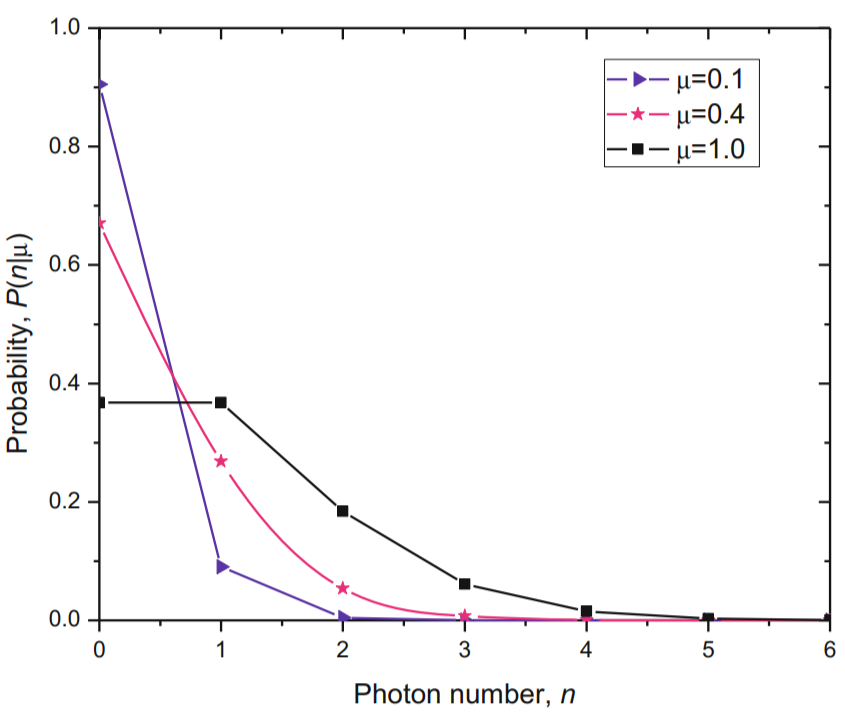
\includegraphics[width=0.7\textwidth]{chapters/figs/fig-7-11}
	\caption{توزیع تعداد فوتون (پواسون) برحسب تعداد فوتون (برای مشاهده روند، توزیع علی‌رغم گسسته بودن به‌صورت پیوسته نشان داده شده است).}
	\label{fig:7-11}
\end{figure}

با افزایش پارامتر $\mu$، احتمال دریافت بیش از یک فوتون نیز افزایش می‌یابد. برای انجام حمله \lr{PNS}، ایو می‌تواند از تقسیم‌کننده پرتو\LTRfootnote{Beam splitter (BS)} برای برداشتن یکی از فوتون‌ها از حالت چندفوتونی استفاده کند و بقیه را به باب انتقال دهد، همان‌طور که در شکل \ref{fig:7-12} تصویر شده است.


\begin{figure}[ht]
	\centering
	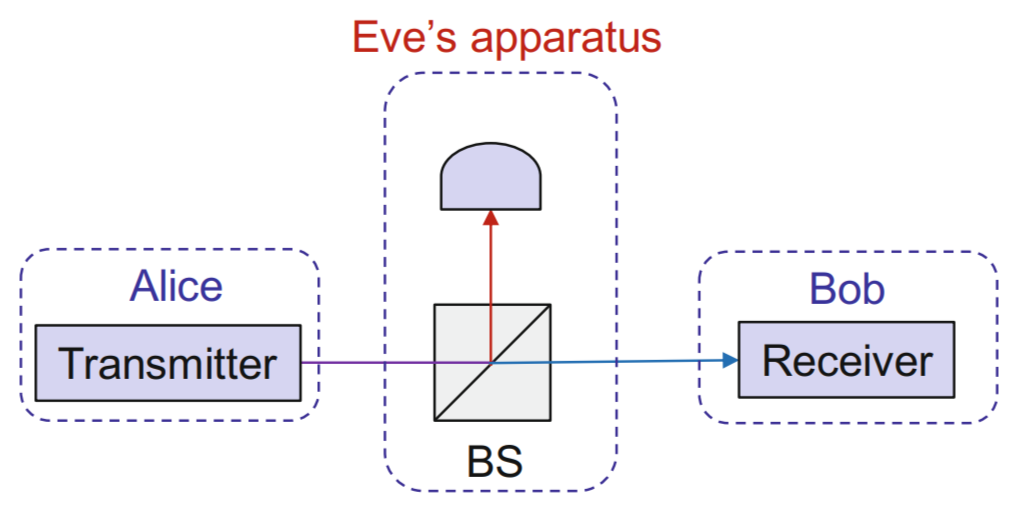
\includegraphics[width=0.6\textwidth]{chapters/figs/fig-7-12}
	\caption{تصویرسازی پیاده‌سازی حمله \lr{PNS} توسط ایو. \lr{BS}: تقسیم‌کننده پرتو.}
	\label{fig:7-12}
\end{figure}


او می‌تواند فوتون را با انتخاب تصادفی پایه اندازه‌گیری کند. ایو حتی می‌تواند پیوند کوانتومی را با فیبر با تلفات بسیار کم جایگزین کند تا آلیس و باب متوجه نشوند که سیگنال ارسالی تضعیف شده است. برای حل مشکل حمله \lr{PNS}، آلیس و باب می‌توانند از یک پروتکل مبتنی بر حالت فریب\LTRfootnote{Decoy state-based} \cite{7-35} استفاده کنند که در آن آلیس حالت‌های کوانتومی را با میانگین تعداد فوتون‌های متفاوت، که نشان‌دهنده حالت‌های سیگنال و فریب هستند، ارسال می‌کند. ایو نمی‌تواند بین حالت فریب و حالت سیگنال تمایز قائل شود و با توجه به اینکه آلیس و باب سطح سیگنال فریب را می‌دانند، می‌توانند حمله \lr{PNS} را شناسایی کنند.








\subsubsection{حملات دسته‌جمعی}
\label{subsec:7-4-1-2}
حملات دسته‌جمعی\LTRfootnote{Collective attacks} نشان‌دهنده تعمیمی از حملات غیرهمدوس هستند، با این فرض که تعامل ایو با هر کیوبیت نیز به‌صورت مستقل و با توزیع یکسان (\lr{i.i.d.}) است. با این حال، در این حملات، ایو می‌تواند کیوبیت‌های کمکی\LTRfootnote{Ancilla qubits} خود را تا پایان مراحل پس‌پردازش کلاسیک در یک حافظه کوانتومی\LTRfootnote{Quantum memory} ذخیره کند. برای مثال، با توجه به اینکه مصالحه اطلاعات مستلزم تبادل بیت‌های توازن روی یک کانال کلاسیک احرازهویت‌شده است، ایو می‌تواند بهترین حملات کلاسیک شناخته‌شده را برای یادگیری محتوای بیت‌های توازن به کار گیرد. بر اساس تمام اطلاعات در دسترس، ایو می‌تواند بهترین استراتژی اندازه‌گیری را روی کیوبیت‌های کمکی خود (ذخیره شده در حافظه کوانتومی) انجام دهد.

حمله \lr{PNS} زمانی که ایو از حافظه کوانتومی استفاده می‌کند قوی‌تر است. به‌ویژه، ایو می‌تواند از طریق فرآیند غربال‌گری متوجه شود که کدام پایه توسط آلیس استفاده شده است و می‌تواند پایه صحیح را روی فوتون ذخیره شده در حافظه کوانتومی خود اعمال کند و در نتیجه تعداد بیت‌های شناسایی شده را در مقایسه با حالتی که از حافظه کوانتومی استفاده نمی‌شود، دوبرابر کند.

کران امنیت برای حملات دسته‌جمعی، با فرض پس‌پردازش یک‌طرفه، توسط رابطه \eqref{eq:7-32} داده می‌شود که در آن اطلاعات ایو درباره دنباله آلیس از طریق اطلاعات هولِوو\LTRfootnote{Holevo information} به‌صورت زیر تعیین می‌شود \cite{7-50} (همچنین ببینید \cite{7-46}):
\begin{equation}
	I_{EA} = \max_{\text{\lr{Eve's strategies}}} \chi(\bm{A}; \bm{E}),
	\label{eq:7-36}
\end{equation}
که در آن بیشینه‌سازی روی تمام استراتژی‌های شنود دسته‌جمعی ممکن انجام می‌شود. تعریف مشابهی برای $I_{BE}$ نیز برقرار است. این کران با نام کران دوتک-وینتر\LTRfootnote{Devetak-Winter bound} نیز شناخته می‌شود. اطلاعات هولِوو که در مرجع \cite{7-51} معرفی شده است، در اینجا به‌صورت زیر تعریف می‌شود:
\begin{equation}
	\chi(\bm{A}; \bm{E}) = S(\rho_E) - \sum_a p(a) S(\rho_{E|a}),
	\label{eq:7-37}
\end{equation}
که در آن $S(\rho)$ آنتروپی فون نویمان\LTRfootnote{von Neumann entropy} است که به‌صورت $S(\rho) = -\text{Tr}(\rho \log \rho) = -\sum_i \lambda_i \log \lambda_i$ تعریف می‌شود و در آن $\lambda_i$ مقادیر ویژه عملگر (حالت) چگالی\LTRfootnote{Density operator} $\rho$ هستند. در رابطه \eqref{eq:7-37}، $p(a)$ نشان‌دهنده احتمال وقوع نماد $a$ از الفبای کلاسیک آلیس است، در حالی که $\rho_{E|a}$ عملگر چگالی متناظر با سیستم کمکی ایو است. در نهایت، $\rho_E$ حالت چگالی جزئی ایو است که به‌صورت $\rho_E = \sum_a p(a) \rho_{E|a}$ تعریف می‌شود. به عبارت دیگر، اطلاعات هولِوو متناظر با میانگین کاهش در آنتروپی فون نویمان است، با این فرض که می‌دانیم $\rho_E$ چگونه آماده‌سازی شده است.

\subsubsection{حملات همدوس}
\label{subsec:7-4-1-3}
حملات همدوس\LTRfootnote{Coherent attacks} نشان‌دهنده کلی‌ترین و منعطف‌ترین استراتژی‌هایی هستند که ایو می‌تواند روی حالت‌های کوانتومی اعمال کند. او می‌تواند استراتژی شنود را در لحظه و بر اساس اندازه‌گیری‌های قبلی و فعلی تطبیق دهد. او ممکن است حالت‌های کوانتومی متعددی را تا جایی که بخواهد درهم‌تنیده کرده و آن‌ها را در حافظه کوانتومی ذخیره کند. بنابراین، کمینه‌سازی اطلاعات متقابل بین آلیس/باب و ایو غیرممکن است. با این وجود، کران‌ها در بسیاری از موارد تعیین شده‌اند و این کران‌ها بسیار شبیه به موارد به‌دست‌آمده برای حملات دسته‌جمعی هستند. به‌ویژه، حالت‌های ارسال شده توسط آلیس $|\psi_i\rangle$ برای باب مستقل هستند و می‌توان آن‌ها را با ضرب تانسوری\LTRfootnote{Tensor product} $|\psi_1\rangle \otimes \dots \otimes |\psi_n\rangle \otimes \dots$ نشان داد و کانال کوانتومی معمولاً بین آن‌ها همبستگی ایجاد نمی‌کند.

بنابراین، ایو با معرفی همبستگی‌های مصنوعی هیچ مزیتی به‌دست نخواهد آورد. با این حال، همبستگی‌ها بعداً در طول پس‌پردازش کلاسیک معرفی می‌شوند و ایو باید به جای حدس زدن نماد ارسال شده در کلید خام، از آن همبستگی‌ها بهره‌برداری کند. کلید نهایی توسط روابط میان نمادها در کلید خام تعیین می‌شود و ایو می‌تواند با به‌کارگیری رویکردهای مبتنی بر درهم‌تنیدگی، برخی از این روابط را بیاموزد.








\subsubsection{حملات هک کوانتومی و/یا حملات کانال جانبی}
\label{subsec:7-4-1-4}
حملات هک کوانتومی\LTRfootnote{Quantum hacking attacks} از نقاط ضعف پیاده‌سازی‌های خاص سیستم‌های \lr{QKD} بهره‌برداری می‌کنند. بسیاری از این حملات با فناوری کنونی امکان‌پذیر هستند. در حمله اسب تروا\LTRfootnote{Trojan horse attack} \cite{7-52}، ایو یک باریکه لیزری درخشان را به سمت رمزگذار آلیس می‌فرستد و فوتون‌های بازتابیده را برای کسب اطلاعات درباره کلید مخفی اندازه‌گیری می‌کند. با استفاده از یک ایزولاتور نوری\LTRfootnote{Optical isolator} می‌توان از این حمله جلوگیری کرد. همچنین مشاهده شده است که شمارنده‌های فوتون مبتنی بر سیلیسیم که از فوتودیودهای بهمنی\LTRfootnote{Avalanche photodiodes (APDs)} (\lr{APD}) استفاده می‌کنند، هنگام آشکارسازی یک تک‌فوتون، مقداری نور در طول‌موج‌های مختلف ساطع می‌کنند که می‌تواند توسط ایو مورد بهره‌برداری قرار گیرد \cite{7-53}. در حمله جابه‌جایی زمانی\LTRfootnote{Time-shifting attack} \cite{7-54}، ایو از عدم تطابق بازدهی آشکارسازهای تک‌فوتون باب برای تخمین انتخاب پایه توسط او استفاده می‌کند. در حمله کورسازی\LTRfootnote{Blinding attack} \cite{7-55}، ایو از ویژگی‌های شمارنده تک‌فوتون مبتنی بر \lr{APD} بهره می‌گیرد تا باب را مجبور کند همان پایه‌ای را انتخاب کند که ایو انتخاب کرده است. \lr{APD}ها برای شمارش فوتون اغلب در مد گیت‌شده\LTRfootnote{Gated mode} عمل می‌کنند، به این معنی که \lr{APD} تنها زمانی فعال است که انتظار ورود فوتون می‌رود. وقتی \lr{APD} در وضعیت غیرفعال (خاموش) است، در یک رژیم خطی\LTRfootnote{Linear regime} عمل می‌کند، به این معنی که جریان نوری با توان نوری دریافتی متناسب است و بنابراین مانند یک فتودتکتور کلاسیک رفتار می‌کند. برای بهره‌برداری از این موضوع، ایو می‌تواند یک باریکه نور کلاسیک ضعیف ارسال کند که به اندازه کافی قوی باشد تا زمانی که باب از همان پایه ایو استفاده می‌کند «کلیک» ایجاد کند، و در غیر این صورت کلیکی ثبت نشود. در چنین سناریویی، $50\%$ از رویدادها به‌صورت بی‌نتیجه\LTRfootnote{Inconclusive} ثبت می‌شوند. خوشبختانه، ویژگی مشترک حملات هک کوانتومی این است که به محض شناخته شدن حمله، قابل پیشگیری هستند. با این حال، تهدید ناشی از حملات هک کوانتومی ناشناخته همچنان پابرجاست.

بسیاری از حملات کانال جانبی\LTRfootnote{Side-channel attacks} به‌طور هم‌زمان حملات خطای صفر\LTRfootnote{Zero-error attacks} هستند \cite{7-46}. به بیان دیگر، ایو می‌تواند از تلفات کانال کوانتومی برای پنهان کردن حمله کانال جانبی خود استفاده کند. حمله تقسیم پرتو\LTRfootnote{Beam-splitting attack} از تلفات کانال کوانتومی بهره‌برداری می‌کند؛ ایو می‌تواند یک تقسیم‌کننده پرتو را دقیقاً بعد از فرستنده آلیس قرار دهد، بخشی از باریکه را برداشته و بقیه را به باب انتقال دهد. از آنجا که آلیس مُد نوری را تغییر نمی‌دهد، این حمله توسط باب شناسایی نخواهد شد. جالب اینجاست که توزیع پواسون در طول حمله \lr{PNS} حفظ می‌شود \cite{7-56}. در پیاده‌سازی‌های واقع‌گرایانه، زمانی که آلیس از حالت‌های سیگنال مستقل خطی استفاده می‌کند، ایو می‌تواند تمایز ابهام‌ناپذیر حالت\LTRfootnote{Unambiguous state discrimination} را انجام داده و متعاقب آن سیگنال را مجدداً ارسال کند و به بازدهی بهتری نسبت به تقسیم پرتو دست یابد، همان‌طور که در مرجع \cite{7-57} نشان داده شده است. خوشبختانه، وجود حملات کانال جانبی تا زمانی که حملات مربوطه در مرحله تقویت حریم خصوصی در نظر گرفته شوند، امنیت را به خطر نمی‌اندازد \cite{7-46}.

\subsection{تعاریف امنیت}
\label{sec:7-4-2}
در اینجا ما به امنیت در برابر حملات دسته‌جمعی علاقه‌مند هستیم. فرض کنید کلید ایده‌آل نشان‌دهنده دنباله‌ای از نمادهای کاملاً همبسته بین آلیس و باب باشد که ایو هیچ اطلاعاتی از آن‌ها ندارد (کلیدهای امن مختلف از مجموعه کلیدهای امن باید به‌صورت یکنواخت ظاهر شوند). در این صورت، کلید $K$ که به اندازه $\epsilon$ از کلید ایده‌آل انحراف داشته باشد، $\epsilon$-امن\LTRfootnote{$\epsilon$-secure} نامیده می‌شود. تعاریف اولیه امنیت \lr{QKD} مشابه تعاریف کلاسیک متناظر بودند. ایو با در اختیار داشتن حالت چگالی $\rho_E$، اندازه‌گیری $\mathcal{M}$ را انجام می‌دهد که اطلاعات متقابل او با $K$ (نشان داده شده با $I(K;E)$) را بیشینه کند. این کار منجر به اطلاعات در دسترس\LTRfootnote{Accessible information} می‌شود و می‌توانیم بنویسیم:
\begin{equation}
	H(\mathcal{K} : E) = \max_{\mathcal{M}(\rho_E)=E} I(\mathcal{K} : E),
	\label{eq:7-38}
\end{equation}
که در آن بیشینه‌سازی روی تمام استراتژی‌های ممکن ایو انجام می‌شود و $H(\mathcal{K} : E)$ نشان‌دهنده اطلاعات در دسترس است. سپس $\epsilon$-امنیت را می‌توان به‌صورت زیر تعریف کرد:
\begin{equation}
	H(\mathcal{K} : E) \leq \epsilon.
	\label{eq:7-39}
\end{equation}
با توجه به اینکه ایو می‌تواند برای انجام اندازه‌گیری روی سیستم خود تا زمانی که بخشی از کلید را یاد بگیرد منتظر بماند، این نامساوی امنیت کلید را تضمین نمی‌کند.

\subsubsection{$\epsilon$-امنیت مبتنی بر فاصله اثر}
\label{subsec:7-4-2-1}
یکی از الزامات کلیدی که تعریف امنیت باید برآورده کند، ویژگی ترکیب‌پذیری\LTRfootnote{Composability} است، که نشان می‌دهد امنیت کلید صرف‌نظر از نوع کاربرد آن تضمین شده است \cite{7-46}. به عبارت دیگر، اگر کلید $\epsilon$-امن در یک وظیفه $\epsilon'$-امن استفاده شود، کل فرآیند باید حداقل $(\epsilon + \epsilon')$-امن باشد. بن-اور\LTRfootnote{Ben-Or} و همکاران در مرجع \cite{7-58} نشان داده‌اند که $\epsilon$-امنیت تعریف شده در رابطه \eqref{eq:7-39} زمانی برقرار است که در مرحله تقویت حریم خصوصی از هشینگ جهانی-$2$\LTRfootnote{Two-universal hashing} استفاده شود. از سوی دیگر، کونیگ\LTRfootnote{König} و همکاران در مرجع \cite{7-59} نشان داده‌اند که اطلاعات در دسترس برای هر $\epsilon$ دلخواه، ترکیب‌پذیر نیست.

برای مقابله با این مشکل، بن-اور و همکاران در \cite{7-58} و همچنین رنر\LTRfootnote{Renner} و کونیگ در \cite{7-60} مفهوم $\epsilon$-امنیت مبتنی بر فاصله اثر\LTRfootnote{Trace-distance-based $\epsilon$-security} را معرفی کردند (همچنین ببینید \cite{7-29, 7-43, 7-61, 7-62, 7-63}). می‌گوییم کلید نسبت به شنودگر $E$ دارای $\epsilon$-امنیت است اگر فاصله اثر بین حالت مشترک کلید $K$ و ایو $E$ (نشان داده شده با $\rho_{K,E}$) و حالت حاصل‌ضربِ حالت کاملاً مخلوط\LTRfootnote{Completely mixed state (CMS)} نسبت به مجموعه $K$ تمام کلیدهای امن ممکن (نشان داده شده با $\rho_{CMS}$) و حالت ایو (نشان داده شده با $\rho_E$)، کوچک‌تر یا مساوی $\epsilon$ باشد. به عبارت دیگر، می‌توانیم بنویسیم:
\begin{equation}
	D(\rho_{K,E}, \rho_{CMS} \otimes \rho_E) = \frac{1}{2} \|\rho_{K,E} - \rho_{CMS} \otimes \rho_E\|_1 = \frac{1}{2} \text{Tr} |\rho_{K,E} - \rho_{CMS} \otimes \rho_E| \leq \epsilon,
	\label{eq:7-40}
\end{equation}
که در آن $|\rho| = \sqrt{\rho^\dagger \rho}$ است. با این تعریف، پارامتر $\epsilon$ تفسیر کاملاً واضحی دارد: این پارامتر نشان‌دهنده حداکثر احتمال شکستِ تحمل‌پذیر برای فرآیند استخراج کلید است. با توجه به اینکه شرط ترکیب‌پذیری در این تعریف برقرار است، می‌توانیم امنیت کلید نهایی $\epsilon$ را برحسب امنیتِ مراحل تصحیح خطا (\lr{EC})\LTRfootnote{Error correction (EC)} $\epsilon_{EC}$، تقویت حریم خصوصی (\lr{PA})\LTRfootnote{Privacy amplification (PA)} $\epsilon_{PA}$ و تخمین پارامتر (\lr{PE})\LTRfootnote{Parameter estimation (PE)} $\epsilon_{PE}$؛ و همچنین احتمال شکستِ تخمین‌های آنتروپی رنی \cite{7-58} (نشان داده شده با $\epsilon_R$) تجزیه کنیم. به عبارت دیگر، می‌توانیم بنویسیم $\epsilon = \epsilon_{EC} + \epsilon_{PA} + \epsilon_{PE} + \epsilon_R$.

اکنون پرسش اصلی این است که چگونه تعریف $\epsilon$-امنیت مبتنی بر فاصله اثر را به طول $m$ کلید مخفی استخراج‌شده مرتبط کنیم. برای این کار، نیاز است نامساوی زیر که نشان‌دهنده تعمیم کران چرنوف\LTRfootnote{Chernoff bound} است، اثبات شود \cite{7-46}:
\begin{equation}
	\text{Pr} \left( D(\rho_{K,E}, \rho_{CMS} \otimes \rho_E) > \epsilon \right) \leq e^{m - f(\rho_{K,E}, \epsilon)},
	\label{eq:7-41}
\end{equation}
که در آن ضرایب ثابت حذف شده‌اند. به‌وضوح، کلید با احتمال بسیار کمی ناامن خواهد بود، به شرطی که شرط زیر برقرار باشد:
\begin{equation}
	m \leq f(\rho_{K,E}, \epsilon).
	\label{eq:7-42}
\end{equation}
به عبارت دیگر، تا زمانی که طول کلید کوتاه‌تر از عدم قطعیت ایو درباره ورودیِ مرحله تقویت حریم خصوصی باشد، کلید امن خواهد بود. کران‌های امنیت بحث شده در بخش \ref{sec:7-4-1} به‌صورت مجانبی برای کلیدهای بی‌نهایت طولانی، زمانی که $\epsilon \to 0$ است، معتبر هستند.








\subsubsection{$\epsilon$-امنیت مبتنی بر وفاداری}
\label{subsec:7-4-2-2}
علاوه بر $\epsilon$-امنیت مبتنی بر فاصله اثر، می‌توان از مفهوم $\epsilon$-امنیت مبتنی بر وفاداری\LTRfootnote{Fidelity-based $\epsilon$-security} نیز استفاده کرد \cite{7-58}. فرض کنیم آلیس دارای $n$ جفت کیوبیت درهم‌تنیده $|B_{00}\rangle = (|00\rangle + |11\rangle)/\sqrt{2}$ باشد که به‌صورت $|B_{00}\rangle^{\otimes n}$ نشان داده می‌شود. وفاداری\LTRfootnote{Fidelity} دو حالت چگالی $\rho$ و $\rho'$ به‌صورت زیر تعریف می‌شود:
\begin{equation}
	F(\rho, \rho') = \text{Tr} \left( \sqrt{\rho^{1/2} \rho' \rho^{1/2}} \right).
	\label{eq:7-43}
\end{equation}
زمانی که $\rho = |\psi\rangle\langle\psi|$ و $\rho' = |\psi'\rangle\langle\psi'|$ حالت‌های خالص باشند، با توجه به اینکه برای حالت‌های خالص $\rho^2 = \rho$ است، وفاداری به‌سادگی به‌صورت زیر در می‌آید:
\begin{equation}
	F(\rho, \rho') = \text{Tr} \sqrt{|\psi\rangle\langle\psi|\psi'\rangle\langle\psi'|\psi\rangle\langle\psi|} = |\langle \psi | \psi' \rangle|.
	\label{eq:7-44}
\end{equation}
وفاداری بین حالت خالص $|\psi\rangle$ و حالت چگالی دلخواه $\rho$ به‌صورت زیر داده می‌شود:
\begin{equation}
	F(\rho, |\psi\rangle) = \text{Tr} \sqrt{|\psi\rangle\langle\psi| \rho |\psi\rangle\langle\psi|} = \text{Tr} \sqrt{\langle\psi|\rho|\psi\rangle |\psi\rangle\langle\psi|} = \sqrt{\langle \psi | \rho | \psi \rangle}.
	\label{eq:7-45}
\end{equation}
یک قضیه مهم مرتبط با وفاداری، قضیه اولمان\LTRfootnote{Uhlmann theorem} است \cite{7-64}، که بیان می‌کند برای دو عملگر چگالی $\rho$ و $\rho'$ و در صورتی که پالایش\LTRfootnote{Purification} حالت $\rho$ به‌صورت $|\psi\rangle\langle\psi|$ باشد، رابطه زیر برقرار است:
\begin{equation}
	F(\rho, \rho') = \max_{|\psi'\rangle\langle\psi'|} F(|\psi\rangle\langle\psi|, |\psi'\rangle\langle\psi'|),
	\label{eq:7-46}
\end{equation}
که در آن بیشینه‌سازی روی تمام پالایش‌های $|\psi'\rangle\langle\psi'|$ از $\rho'$ انجام می‌شود. با اعمال رابطه \eqref{eq:7-45} روی $|B_{00}\rangle^{\otimes n}$، به‌دست می‌آوریم:
\begin{equation}
	F^2(\rho_{AB}^n, |B_{00}\rangle^{\otimes n}) = \prescript{\otimes n}{}{\langle} B_{00} | \rho_{AB}^n | B_{00} \rangle^{\otimes n},
	\label{eq:7-47}
\end{equation}
که در آن $\rho_{AB}^n$ حالت چگالی مشترک بین آلیس و باب است. کلیدهای نهایی برای آلیس و باب که به‌ترتیب با $\mathcal{K}_A$ و $\mathcal{K}_B$ نشان داده می‌شوند، دارای طول $m < n$ هستند و در غیاب ایو، $\rho_{AB}^m$ برابر با $|B_{00}\rangle^{\otimes m}$ خواهد بود. بنابراین، می‌توانیم $\epsilon$-امنیت مبتنی بر وفاداری را به‌صورت زیر تعریف کنیم:
\begin{equation}
	1 - F(\rho_{AB}^m, |B_{00}\rangle^{\otimes m}) \leq \epsilon''.
	\label{eq:7-48}
\end{equation}
بنابراین در غیاب ایو، $F(\rho_{AB}^m, |B_{00}\rangle^{\otimes m}) = 1$ است و به‌وضوح در آن حالت $0 = \epsilon''$ خواهد بود. فرض کنید $|\psi_1^m\rangle\langle\psi_1^m|$ پالایش $\rho_{ABE}^m$ روی سیستم‌های $A$، $B$ و $E$ باشد. طبق قضیه اولمان، پالایشی مانند $|\psi_1^m\rangle\langle\psi_1^m|$ وجود دارد به‌طوری که:
\begin{equation}
	F(|\psi_1^m\rangle\langle\psi_1^m|, |\psi_2^m\rangle\langle\psi_2^m|) = F(\rho_{AB}^m, |B_{00}\rangle^{\otimes m}).
	\label{eq:7-49}
\end{equation}
با ساخت مناسب حالت‌های پالایش $|\psi_1^m\rangle$ و $|\psi_2^m\rangle$ و انجام اندازه‌گیری‌ها روی سیستم آلیس و باب، در حالی که اثر جزئی روی سیستم ایو گرفته می‌شود، به‌دست می‌آوریم:
\begin{equation}
	F(\rho_{\text{QKD}}^m, \rho_{\text{perfect}}^m) > F(\rho_{AB}^m, |B_{00}\rangle^{\otimes m}),
	\label{eq:7-50}
\end{equation}
که در آن $\rho_{\text{perfect}}^m$ عملگر چگالی متناظر با کلید ایده‌آل\LTRfootnote{Perfect key} است؛ کلیدی که توزیع آن روی دو رشته به طول $m$ به‌صورت $p_{\text{perfect}}^{(m)}(l, l') = \delta(l, l') 2^{-m}$ است \cite{7-58}. در رابطه \eqref{eq:7-50}، $\rho_{\text{QKD}}^m$ نشان‌دهنده عملگر چگالی متناظر با طرح \lr{QKD} است. به عبارت دیگر، با انجام پالایش دو حالت چگالی، وفاداری بهبود می‌یابد. با توجه به اینکه فاصله اثر و وفاداری طبق مراجع \cite{7-6, 7-61} با هم مرتبط هستند:
\begin{equation}
	\|\rho_{\text{QKD}}^m - \rho_{\text{perfect}}^m\|_1 \leq 2 \sqrt{1 - F(\rho_{\text{QKD}}^m, \rho_{\text{perfect}}^m)},
	\label{eq:7-51}
\end{equation}
نتیجه می‌گیریم که $\epsilon$-امنیت مبتنی بر وفاداری با $\epsilon$-امنیت مبتنی بر فاصله اثر مرتبط است، زیرا:
\begin{equation}
	\frac{1}{2} \|\rho_{\text{QKD}}^m - \rho_{\text{perfect}}^m\|_1 \leq \sqrt{\epsilon''},
	\label{eq:7-52}
\end{equation}
و بنابراین تعریف $\epsilon$-امنیت مبتنی بر وفاداری نیز ترکیب‌پذیر\LTRfootnote{Composable} است.

اگر وفاداری بالا باشد، آنگاه عدد صحیح مثبت $s$ وجود دارد به‌طوری که:
\begin{equation*}
	F^2(\rho_{AB}^m, |B_{00}\rangle^{\otimes m}) = \prescript{\otimes m}{}{\langle} B_{00} | \rho_{AB}^m | B_{00} \rangle^{\otimes m} > 1 - 2^{-s}.
\end{equation*}
به‌وضوح، بزرگ‌ترین مقدار ویژه $\rho_{AB}^m$ باید بزرگ‌تر از $1 - 2^{-s}$ باشد. آنتروپی فون نویمان\LTRfootnote{von Neumann entropy} برای $\rho_{AB}^m$ از بالا توسط آنتروپی عملگر چگالی زیر محدود می‌شود \cite{7-6}:
\begin{equation}
	\bm{\rho}_{\max} = \text{diag} \left( 1 - 2^{-s}, \underbrace{\frac{2^{-s}}{2^{2m}-1}, \dots, \frac{2^{-s}}{2^{2m}-1}}_{2^{2m}-1 \text{ entries}} \right)
	\label{eq:7-53}
\end{equation}
که به‌صورت زیر داده می‌شود:
\begin{equation}
	S_{\max} = S(\bm{\rho}_{\max}) = -(1 - 2^{-s}) \log(1 - 2^{-s}) - (2^{2n} - 1) \frac{2^{-s}}{2^{2m}-1} \log \left( \frac{2^{-s}}{2^{2m}-1} \right).
	\label{eq:7-54}
\end{equation}
با استفاده از تقریب $x \approx \ln(1+x)$ زمانی که $x$ کوچک باشد، به‌دست می‌آوریم:
\begin{equation}
	S_{\max} \leq (1 - 2^{-s}) 2^{-s} / \ln 2 + 2^{-s}s + 2^{-s}2m = (2m + s + 1/\ln 2) 2^{-s} - \underbrace{\frac{2^{-2s}}{\ln 2}}_{O(2^{-2s})}.
	\label{eq:7-55}
\end{equation}
در نتیجه، وفاداری بالا به معنای آنتروپی فون نویمان پایین است زیرا:
\begin{equation}
	S(\rho_{AB}^m) < S_{\max} \leq (2m + s + 1/\ln 2) 2^{-s} - O(2^{-2s}).
	\label{eq:7-56}
\end{equation}
بنابراین، با حصول اطمینان از اینکه آلیس و باب جفت‌های \lr{EPR} با وفاداری حداقل $1 - 2^{-s}$ در اختیار دارند، پروتکل \lr{QKD} امن خواهد بود \cite{7-6}.




\subsubsection{نرخ‌های کلید امن برای سیستم‌های \lr{DV-QKD} دوبعدی}
\label{subsec:7-4-3}
کران مربوط به طرح‌های \lr{DV-QKD} دوبعدی (\lr{2-D})، با فرض حملات انفرادی، توسط روابط \eqref{eq:7-32} و \eqref{eq:7-33} داده می‌شود. اطلاعات متقابل بین آلیس و باب را می‌توان با به‌کارگیری کانال متقارن باینری\LTRfootnote{Binary symmetric channel (BSC)} (\lr{BSC}) تعیین کرد، که در آن برای احتمال خطای $q$، که در \lr{DV-QKD} معمولاً نرخ خطای بیت کوانتومی\LTRfootnote{Quantum bit-error rate (QBER)} (\lr{QBER}) نامیده می‌شود، اطلاعات متقابل به‌صورت $I(A; B) = 1 - h(q)$ تعیین می‌گردد. برای در نظر گرفتن گام ناقص مصالحه اطلاعات، یا به‌طور معادل کدگذاری کنترل خطا\LTRfootnote{Error control coding (ECC)} (\lr{ECC})، نشت اطلاعات \lr{ECC} به ایو که با $\text{leakage}_{\text{ECC}}(q)$ نشان داده می‌شود \cite{7-46}، به‌وضوح از پایین توسط $h(q)$ محدود می‌گردد؛ بنابراین می‌توانیم عبارت \lr{SKR} را به‌صورت زیر بازنویسی کنیم:
\begin{equation}
	\text{SKR} = R_{\text{raw}} [1 - \text{leakage}_{\text{ECC}}(q) - I_E], \quad I_E = \min_{\text{Eve's strategies}} (I_{EA}, I_{EB}).
	\label{eq:7-57}
\end{equation}
عبارتی مشابه این در مراجع \cite{7-65, 7-66, 7-67, 7-68} استخراج شده است. ما فرض می‌کنیم که ایو تنها می‌تواند برای بازه‌های زمانی غیرخالی اطلاعات کسب کند، به شرطی که باب آنچه را که ایو برای او مجدداً ارسال کرده است، آشکارسازی کند. با توجه به اینکه منبع آلیس را می‌توان به‌صورت ارسال پالسی حاوی $n$ فوتون با احتمال $p_{A,n}$ بازنمایی کرد، می‌توانیم قضیه دِ فینتی\LTRfootnote{de Finetti theorem} \cite{7-61} را اعمال کنیم؛ در این صورت می‌توانیم اطلاعات ایو $I_E$ را برحسب $I_E$ برای هر تعداد فوتون به‌صورت زیر تجزیه کنیم:
\begin{equation}
	I_E = \min(I_{EA}, I_{EB}) = \min_{\text{Eve's strategies}} \left\{ \max \left( \sum_n I_{EA,n} y_n \right), \max \left( \sum_n I_{EB,n} y_n \right) \right\},
	\label{eq:7-58}
\end{equation}
که در آن $y_n = R_{\text{raw},n}/R_{\text{raw}}$ است و نشان‌دهنده کسرِ نرخ کلید خام کل در زمانی است که آلیس از $n$ فوتون در هر پالس استفاده کرده است.





\subsubsection{پروتکل BB84 آماده‌سازی-و-اندازه‌گیری}
\label{subsec:7-4-3-1}
در پروتکل \lr{BB84} آماده‌سازی-و-اندازه‌گیری\LTRfootnote{Prepare-and-measure}، $I_{EA} = I_{EB}$ است و عبارت \eqref{eq:7-58} به صورت $I_E = \max (\sum_{n} I_{EA,n} y_n)$ ساده می‌شود. در حالت صفر-فوتونی، واضح است که $I_{EA,0} = 0$ است. برای حالت تک-فوتونی، تنها راهی که ایو می‌تواند مقداری اطلاعات کسب کند، به‌کارگیری حمله سد کردن-بازارسال\LTRfootnote{Intercept-resend (IR)} است که نرخ خطای $q_1$ را معرفی می‌کند و اطلاعات متناظر ایو $I_{EA,1} = h(q_1)$ خواهد بود. برای تعداد فوتون‌های دو و بیشتر در هر پالس، ایو از حمله \lr{PNS} استفاده می‌کند و اطلاعات او در این حالت برابر با $1$ است، یعنی $I_{EA,n} = 1$ برای $n \geq 2$. به‌وضوح، بر اساس این بحث، نتیجه می‌گیریم که اطلاعات ایو به‌صورت زیر خواهد بود:
\begin{equation}
	\begin{aligned}
		I_E &= \max_{\text{Eve's strategies}} \sum_{n} I_{EA,n} y_n = \max_{\text{Eve's strategies}} [y_1 h(q_1) + y_{n \geq 2}] \\
		&= \max_{\text{Eve's strategies}} [y_1 h(q_1) + 1 - y_0 - y_1] = 1 - \min_{\text{Eve's strategies}} \{ y_0 + y_1 [1 - h(q_1)] \}.
	\end{aligned}
	\label{eq:7-59}
\end{equation}
در طرح‌های \lr{QKD} دوبعدی آماده‌سازی-و-اندازه‌گیری، مانند \lr{BB84}، تنها پارامترهایی که اندازه‌گیری می‌شوند نرخ کلید خام $R_{\text{raw}} = \sum_n R_{\text{raw},n}$ و میانگین نرخ خطای بیت کوانتومی (\lr{QBER}) $q = \sum_n q_n y_n$ هستند. در این صورت، باید فرض کنیم که برای $n \geq 2$ مقدار $q_n = 0$ است، به‌طوری که $q_1 = q/y_1$ شود. علاوه‌بر این، در رابطه \eqref{eq:7-31} منطقی است که $p_0 = 0$ و برای $n \geq 2$ مقدار $p_n = 0$ قرار داده شود تا بتوانیم بنویسیم:
\begin{equation}
	R_{\text{raw}} = R_{\text{raw},1} + R_{\text{raw},n \geq 2} = R_{\text{raw},1} + R_s p_{\text{sift}} p_{A,n \geq 2},
	\label{eq:7-60}
\end{equation}
و پس از تقسیم هر دو طرف معادله بر $R_{\text{raw}}$، راه حل زیر را برای $y_1 = R_{\text{raw},1}/R_{\text{raw}}$ به‌دست می‌آوریم \cite{7-68}:
\begin{equation}
	y_1 = 1 - (R_s/R_{\text{raw}}) p_{\text{sift}} p_{A,n \geq 2}.
	\label{eq:7-61}
\end{equation}
برای این $y_1$، رابطه \eqref{eq:7-59} به‌صورت زیر در می‌آید:
\begin{equation}
	I_E = 1 - y_1 [1 - h(q_1)] = 1 - y_1 [1 - h(q/y_1)].
	\label{eq:7-62}
\end{equation}
در نهایت، پس از جایگذاری $I_E$ استخراج‌شده در رابطه \eqref{eq:7-57}، معادله زیر را برای \lr{SKR} به‌دست می‌آوریم:
\begin{equation}
	\text{SKR} = R_{\text{raw}} [y_1 (1 - h(q/y_1)) - \text{leakage}_{\text{ECC}}(q)].
	\label{eq:7-63}
\end{equation}

\subsubsection{پروتکل مبتنی بر حالت فریب}
\label{subsec:7-4-3-2}
در ادامه این بخش، \lr{QKD} دوبعدی را با استفاده از حالت‌های فریب\LTRfootnote{Decoy states} مطالعه می‌کنیم \cite{7-35, 7-69, 7-70, 7-71, 7-72, 7-73, 7-74, 7-75, 7-76}. در پروتکل‌های مبتنی بر حالت فریب، آلیس ماهیت سیگنال کوانتومی (مانند شدت لیزر) را به‌طور تصادفی تغییر می‌دهد. در پایان فرآیند ارسال، او فاش می‌کند که از چه شدت‌هایی استفاده کرده است تا ایو نتواند حمله خود را در حین اجرا تطبیق دهد. در مرحله پس‌پردازش، آلیس و باب از این اطلاعات برای تخمین پارامتر استفاده می‌کنند. آلیس و باب می‌توانند کسر مخفی را با بهینه‌سازی هم روی سطوح سیگنال و هم روی احتمال وقوع هر سطح، بیشینه کنند. در عمل، حتی در حضور اثرات تلاطم اتمسفری، همان‌طور که در \cite{7-77} نشان داده شده است، سه سطح کافی می‌باشد. فرض کنید $p$ برخی پارامترهای منبع باشد که قابل تنظیم هستند، مانند میانگین تعداد فوتون $\mu$ (یا شدت) منبع لیزر. آلیس مقدار پارامتر $p$ را به‌طور تصادفی از پالس به پالس تغییر می‌دهد و در پایان فاز ارسال کلید خام، فهرست مقادیر $p \in \mathcal{P}$ را فاش می‌کند. آلیس و باب داده‌های موجود را دسته‌بندی کرده و تخمین پارامتر را انجام می‌دهند. آلیس و باب $2|\mathcal{P}|$ پارامتر $R_{\text{raw}}^{(p)}$ و $q^{(p)}$ را برای $p = 1, \dots, |\mathcal{P}|$ اندازه‌گیری می‌کنند. مجموعه پارامترهای $\mathcal{P}$ به‌صورت عمومی شناخته می‌شود؛ با این حال، برای $|\mathcal{P}| > 1$ ایو نمی‌تواند استراتژی اندازه‌گیری خود را بر اساس $p$ تطبیق دهد، زیرا از قبل آن را نمی‌داند. بدیهی است که $p_n$ و $q_n$ مستقل از $p$ هستند. نرخ کلید خام زمانی که آلیس پالسی با $n$ فوتون ارسال می‌کند به‌صورت $R_{\text{raw},n}^{(p)} = R_s p_{\text{sift}} p_{A,n}^{(p)} p_n$ می‌شود. پارامترهای اندازه‌گیری شده به‌صورت زیر در می‌آیند:
\begin{equation}
	R_{\text{raw}}^{(p)} = \sum_{n \geq 0} R_{\text{raw},n}^{(p)}, \quad q^{(p)} = \sum_{n \geq 0} q_n^{(p)} y_n^{(p)}; \quad p = 1, 2, \dots, |\mathcal{P}|
	\label{eq:7-64}
\end{equation}
معادله فوق یک سیستم خطی از $2|\mathcal{P}|$ معادله برای $p_n$ و $q_n$ معرفی می‌کند. همان‌طور که در بالا ذکر شد، در عمل پروتکل حالت فریب با $|\mathcal{P}| = 3$ عملکردی قابل مقایسه با حالت ایده‌آل دارد \cite{7-76, 7-77}. برای هر $p$، اطلاعات ایو به‌صورت زیر داده می‌شود:
\begin{equation}
	I_E^{(p)} = 1 - y_0^{(p)} - y_1^{(p)} [1 - h(q_1)]; \quad y_n^{(p)} = R_{\text{raw},n}^{(p)}/R_{\text{raw}}^{(p)}, \quad n = 0, 1
	\label{eq:7-65}
\end{equation}
\lr{SKR} کل را می‌توان با جمع کردن \lr{SKR}ها برای مقادیر مختلف $p$ به‌دست آورد، یعنی $\text{SKR} = \sum_p \text{SKR}^{(p)}$. هنگامی که پس‌پردازش کلاسیک روی کل کلید خام اعمال شده باشد، \lr{SKR} به‌صورت زیر ساده می‌شود:
\begin{equation}
	\text{SKR} = R_{\text{raw}} [1 - \text{leakage}_{\text{ECC}}(q)] - \sum_p R_{\text{raw}}^{(p)} I_E^{(p)}.
	\label{eq:7-66}
\end{equation}






\section{مبانی اپتیک کوانتومی}
\label{sec:7-5}
در این بخش، برای تسهیل در تشریح طرح‌های \lr{CV-QKD}، به‌اختصار مبانی اپتیک کوانتومی \cite{7-7, 7-30, 7-78, 7-79, 7-80} را شرح می‌دهیم. برای مطالعه توصیف تفصیلی اپتیک کوانتومی، خواننده علاقه‌مند به فصل \ref{chap:6} ارجاع داده می‌شود. یک موج تخت تک‌فام\LTRfootnote{Monochromatic plane wave} را می‌توان به‌صورت زیر نمایش داد:
\begin{equation}
	\bm{E}(\bm{r}, t) = \bm{e} |\bm{E}| [I \cos(\bm{k}\bm{r} - \omega t) - Q \sin(\bm{k}\bm{r} - \omega t)]
	\label{eq:7-67}
\end{equation}
که در آن مؤلفه اول نشان‌دهنده هم‌فاز\LTRfootnote{In-phase} و مؤلفه دوم نشان‌دهنده مؤلفه مربعی\LTRfootnote{Quadrature component} است. بردار $\bm{e}$ جهت‌گیری قطبش را نشان می‌دهد، $\bm{k}$ بردار موج و $\bm{r}$ بردار مکان است.

\subsection{عملگرهای مربعی، عملگرهای تولید و نابودی، اصل عدم قطعیت}
\label{subsec:7-5-1}
در اپتیک کوانتومی، مؤلفه‌های مربعی $I$ و $Q$ با عملگرهای متناظر $\hat{I}$ و $\hat{Q}$ جایگزین می‌شوند که معادل عملگرهای مکان و تکانه هستند و در رابطه جابه‌جایی مشابهی صدق می‌کنند:
\begin{equation}
	[\hat{I}, \hat{Q}] = 2jN_0,
	\label{eq:7-68}
\end{equation}
که در آن $N_0$ نشان‌دهنده واریانس نوسان خلأ (نویز شات\LTRfootnote{Shot noise}) است. (اغلب در اپتیک کوانتومی، نمادگذاری متفاوتی برای عملگرهای مربعی استفاده می‌شود؛ به‌ویژه به جای آن‌ها از $\hat{x}$ و $\hat{p}$ استفاده می‌گردد.) حالت‌های ویژه $\hat{I}$ را می‌توان با $|I\rangle$ نشان داد، زیرا $\hat{I}|I\rangle = I|I\rangle$ است.
عملگرهای نابودی\LTRfootnote{Annihilation operator} $a$ و تولید\LTRfootnote{Creation operator} $a^\dagger$ به‌صورت زیر تعریف می‌شوند:
\begin{equation}
	a = \frac{\hat{I} + j\hat{Q}}{2\sqrt{N_0}}, \quad a^\dagger = \frac{\hat{I} - j\hat{Q}}{2\sqrt{N_0}}.
	\label{eq:7-69}
\end{equation}
به عبارت دیگر، می‌توانیم عملگرهای مربعی را برحسب عملگرهای نابودی و تولید به‌صورت زیر بیان کنیم:
\begin{equation}
	\hat{I} = (a^\dagger + a)\sqrt{N_0}, \quad \hat{Q} = j(a^\dagger - a)\sqrt{N_0}.
	\label{eq:7-70}
\end{equation}
عملگر تعداد فوتون پیش‌تر به‌صورت زیر معرفی شده بود:
\begin{equation}
	\hat{N} = a^\dagger a = \frac{\hat{I} + j\hat{Q}}{2\sqrt{N_0}} \frac{\hat{I} - j\hat{Q}}{2\sqrt{N_0}} = \frac{1}{4N_0} \left[ (\hat{I}^2 + \hat{Q}^2) - j \underbrace{(\hat{I}\hat{Q} - \hat{Q}\hat{I})}_{[\hat{I}, \hat{Q}] = 2N_0 j} \right] = \frac{1}{4N_0} [(\hat{I}^2 + \hat{Q}^2) + 2N_0],
	\label{eq:7-71}
\end{equation}
حالت‌های فوک\LTRfootnote{Fock states} (حالت‌های تعداد فوتون) کِت‌های ویژه عملگر تعداد فوتون هستند:
\begin{equation}
	\hat{N}|n\rangle = n|n\rangle,
	\label{eq:7-72}
\end{equation}
که در آن $n$ نشان‌دهنده تعداد فوتون‌ها است.
حالت خلأ\LTRfootnote{Vacuum state} که با $|0\rangle$ نشان داده می‌شود، یک کِت ویژه از عملگر نابودی است:
\begin{equation}
	a|0\rangle = 0 \Rightarrow \langle 0 | a^\dagger a | 0 \rangle = 0.
	\label{eq:7-73}
\end{equation}
حالت همدوس $| \alpha \rangle$ که پیش‌تر معرفی شد، کِت ویژه راستِ عملگر نابودی $a$ است؛ یعنی $a|\alpha\rangle = \alpha|\alpha\rangle$ که در آن $\alpha$ مقدار ویژه مختلط است. مقادیر چشم‌داشتی\LTRfootnote{Expected values} عملگرهای مربعی نسبت به حالت $|\alpha\rangle$ به‌صورت زیر داده می‌شوند:
\begin{equation}
	\begin{aligned}
		\langle \hat{I} \rangle_\alpha &= \langle \alpha | \hat{I} | \alpha \rangle = \langle \alpha | (a + a^\dagger) | \alpha \rangle \sqrt{N_0} = \langle \alpha | (\alpha + \alpha^*) | \alpha \rangle \sqrt{N_0} = 2\text{Re}\{\alpha\}\sqrt{N_0}, \\
		\langle \hat{Q} \rangle_\alpha &= \langle \alpha | \hat{Q} | \alpha \rangle = j\langle \alpha | (a^\dagger - a) | \alpha \rangle \sqrt{N_0} = j\langle \alpha | (\alpha^* - \alpha) | \alpha \rangle \sqrt{N_0} = 2\text{Im}\{\alpha\}\sqrt{N_0}.
	\end{aligned}
	\label{eq:7-74}
\end{equation}
بنابراین، اگر ضریب مقیاس $1/(2\sqrt{N_0})$ را بر $\alpha$ اعمال کنیم، مقادیر چشم‌داشتی عملگرهای هم‌فاز و مربعی نشان‌دهنده بخش‌های حقیقی و موهومی $\alpha$ خواهند بود. برای حالت خلأ، مقادیر چشم‌داشتی عملگرهای مربعی برابر با صفر است و بنابراین، رابطه \eqref{eq:7-74} جابه‌جایی\LTRfootnote{Displacement} را تعریف می‌کند. مقادیر چشم‌داشتی $\hat{I}^2$ و $\hat{Q}^2$ به‌صورت زیر داده می‌شوند:
\begin{equation}
	\begin{aligned}
		\langle \hat{I}^2 \rangle_\alpha &= \langle \alpha | \hat{I}^2 | \alpha \rangle = \langle \alpha | (a + a^\dagger)(a + a^\dagger) | \alpha \rangle N_0 = [(\alpha + \alpha^*)^2 + 1] N_0, \\
		\langle \hat{Q}^2 \rangle_\alpha &= \langle \alpha | \hat{Q}^2 | \alpha \rangle = j^2 \langle \alpha | (a^\dagger - a)(a^\dagger - a) | \alpha \rangle N_0 = [1 - (\alpha^* - \alpha)^2] N_0.
	\end{aligned}
	\label{eq:7-75}
\end{equation}
واریانس‌های متناظر برای عملگرهای مربعی در این صورت برابر خواهند بود با:
\begin{equation}
	\begin{aligned}
		\langle \Delta \hat{I}^2 \rangle_\alpha &= \langle \hat{I}^2 \rangle_\alpha - \langle \hat{I} \rangle_\alpha^2 = [(\alpha + \alpha^*)^2 + 1] N_0 - (\alpha + \alpha^*)^2 N_0 = N_0, \\
		\langle \Delta \hat{Q}^2 \rangle_\alpha &= \langle \hat{Q}^2 \rangle_\alpha - \langle \hat{Q} \rangle_\alpha^2 = [1 - (\alpha^* - \alpha)^2] N_0 + (\alpha^* - \alpha)^2 N_0 = N_0,
	\end{aligned}
	\label{eq:7-76}
\end{equation}
که نشان می‌دهد واریانس‌های نوسانات برای هر دو مؤلفه مربعی یکسان است. با قرار دادن $\alpha = 0$، همین نتیجه برای حالت خلأ نیز صدق می‌کند. حاصل‌ضرب واریانس‌های مؤلفه‌های مربعی به‌صورت زیر داده می‌شود:
\begin{equation}
	\langle \Delta \hat{I}^2 \rangle_\alpha \langle \Delta \hat{Q}^2 \rangle_\alpha = N_0^2,
	\label{eq:7-77}
\end{equation}
که نشان می‌دهد اصل عدم قطعیت هایزنبرگ با علامت تساوی برقرار است. به عبارت دیگر، حالت همدوس در رابطه کمینه عدم قطعیت صدق می‌کند. اصل عدم قطعیت در سیستم‌های \lr{CV-QKD} به‌کار گرفته می‌شود. اغلب اصل عدم قطعیت برحسب واحد نویز شات\LTRfootnote{Shot noise unit (SNU)} بیان می‌شود، جایی که $N_0$ به $1$ نرمالیزه شده است، به‌صورت زیر: $\Delta \hat{I}^2 \Delta \hat{Q}^2 \geq 1$.






\subsection{حالت‌های همدوس، حالت گاوسی و حالت‌های فشرده}
\label{subsec:7-5-2}
حالت گاوسی\LTRfootnote{Gaussian state} یک حالت همدوس است که در آن تصویرها در امتداد کِت‌های ویژه $\hat{I}$ دارای شکل گاوسی هستند:
\begin{equation}
	\langle I|\alpha \rangle = \frac{1}{(2\pi N_0)^{1/4}} \exp\left[ -\frac{(I-\langle I \rangle)^2 + j\langle I \rangle \langle Q \rangle}{4N_0} + \frac{j I \langle Q \rangle}{2N_0} \right].
	\label{eq:7-78}
\end{equation}
حالت فشرده\LTRfootnote{Squeezed state} یک حالت گاوسی خاص است که دارای نوسانات نابرابر در مؤلفه‌های مربعی\LTRfootnote{Quadratures} است:
\begin{equation}
	\begin{aligned}
		\langle I|\alpha, s \rangle = \frac{1}{(2\pi N_0 s)^{1/4}} \exp\left[ -\frac{s^{-1}(I-\langle I \rangle)^2 + j\langle I \rangle \langle Q \rangle}{4N_0} + \frac{j I \langle Q \rangle}{2N_0} \right], \quad s > 0 \\
		V(\hat{I}) = \text{Var}(\hat{I}) = sN_0, \quad V(\hat{Q}) = \text{Var}(\hat{Q}) = s^{-1} N_0,
	\end{aligned}
	\label{eq:7-79}
\end{equation}
که در آن $s$ پارامتر فشردگی\LTRfootnote{Squeezing parameter} است.
برای تجسم حالت‌های کوانتومی در اپتیک کوانتومی، از تابع ویگنر\LTRfootnote{Wigner function} استفاده می‌شود که برای حالت چگالی\LTRfootnote{Density state} $\rho$ به‌صورت زیر تعریف می‌گردد \cite{7-7}:
\begin{equation}
	W(I, Q) = \frac{1}{4\pi N_0} \int e^{\frac{j \xi Q}{2N_0}} \langle I - \xi/2 | \rho | I + \xi/2 \rangle d\xi.
	\label{eq:7-80}
\end{equation}
اگر کسی مؤلفه هم‌فاز را اندازه‌گیری کند، نتیجه از تابع چگالی احتمال\LTRfootnote{Probability density function (PDF)} (\lr{PDF}) $f(I)$ پیروی می‌کند که با میانگین‌گیری از تابع ویگنر روی مؤلفه مربعی به‌دست می‌آید، یعنی $f(I) = \int W(I, Q) dQ$. از سوی دیگر، اگر کسی مؤلفه مربعی را اندازه‌گیری کند، نتیجه از \lr{PDF} مقابل پیروی خواهد کرد: $f(Q) = \int W(I, Q) dI$. بنابراین، می‌توانیم تابع ویگنرِ حالت همدوس $|\alpha\rangle$ را به‌عنوان یک توزیع گاوسی دو‌بعدی به مرکزیت $(\text{Re}\{\alpha\}, \text{Im}\{\alpha\})$ با واریانس $N_0$ (و کوواریانس صفر) تفسیر کنیم. در نتیجه، در صفحه $(I, Q)$ حالت همدوس توسط یک دایره نمایش داده می‌شود که شعاع آن با انحراف معیار (عدم قطعیت) مرتبط است، همان‌طور که در شکل \ref{fig:7-13} تصویر شده است.






\begin{figure}[ht]
	\centering
	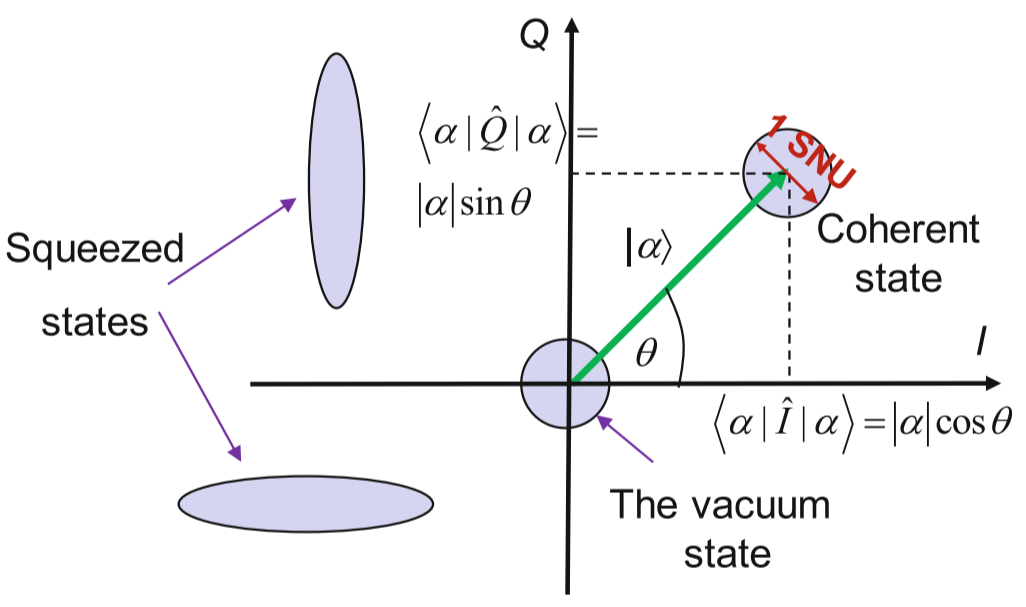
\includegraphics[width=0.8\textwidth]{chapters/figs/fig-7-13}
	\caption{تصویرسازی حالت‌های همدوس و فشرده.}
	\label{fig:7-13}
\end{figure}








در حالت‌های فشرده، مختصات $I$ با ضریب $s^{1/2}$ و مختصات $Q$ با ضریب $s^{-1/2}$ مقیاس‌بندی می‌شوند.
اکنون بیایید حالت همدوس را برحسب حالت‌های تعداد بیان کنیم. با استفاده از رابطه کامل بودن\LTRfootnote{Completeness relationship}، می‌توانیم بنویسیم:
\begin{equation}
	|\alpha\rangle = \sum_n (|n\rangle \langle n |) | \alpha \rangle = \sum_n |n\rangle \langle n|\alpha\rangle.
	\label{eq:7-81}
\end{equation}
از آنجا که حالت تعداد $|n\rangle$ را می‌توان برحسب حالت پایه\LTRfootnote{Ground state} به‌صورت زیر نمایش داد \cite{7-81}:
\begin{equation}
	|n\rangle = \frac{(a^\dagger)^n}{\sqrt{n!}} |0\rangle,
	\label{eq:7-82}
\end{equation}
ضریب تصویر را می‌توان به‌صورت زیر تعیین کرد:
\begin{equation}
	\langle n|\alpha\rangle = \langle 0 | \frac{a^n}{\sqrt{n!}} |\alpha\rangle = \frac{\alpha^n}{\sqrt{n!}} \langle 0|\alpha\rangle,
	\label{eq:7-83}
\end{equation}
و حالت همدوس پس از جایگذاری \eqref{eq:7-83} در \eqref{eq:7-81} به‌صورت زیر در می‌آید:
\begin{equation}
	|\alpha\rangle = \langle 0|\alpha\rangle \sum_n \frac{\alpha^n}{\sqrt{n!}} |n\rangle.
	\label{eq:7-84}
\end{equation}
تصویر در امتداد حالت پایه $\langle 0|\alpha\rangle$ را می‌توان از شرط هنجاریدگی\LTRfootnote{Normalization condition} تعیین کرد:
\begin{equation}
	1 = \sum_n |\langle n|\alpha\rangle|^2 = \sum_n \frac{|\langle 0|\alpha\rangle|^2 |\alpha|^{2n}}{n!} = |\langle 0|\alpha\rangle|^2 e^{|\alpha|^2},
	\label{eq:7-85}
\end{equation}
و با حل برای $\langle 0|\alpha\rangle$ به‌دست می‌آوریم:
\begin{equation}
	\langle 0|\alpha\rangle = e^{-|\alpha|^2/2},
	\label{eq:7-86}
\end{equation}
و پس از جایگذاری \eqref{eq:7-86} در \eqref{eq:7-84}، حالت همدوس به‌صورت زیر نمایش می‌یابد:
\begin{equation}
	|\alpha\rangle = e^{-|\alpha|^2/2} \sum_n \frac{\alpha^n}{\sqrt{n!}} |n\rangle.
	\label{eq:7-87}
\end{equation}
شکل مناسب دیگری را می‌توان با بیان عملگر تعداد برحسب حالت پایه، بر اساس رابطه \eqref{eq:7-82} به‌دست آورد:
\begin{equation}
	|\alpha\rangle = e^{-|\alpha|^2/2} \sum_n \frac{\alpha^n}{n!} (a^\dagger)^n |0\rangle = e^{-|\alpha|^2/2} e^{\alpha a^\dagger} |0\rangle = e^{\alpha a^\dagger - \alpha^* a} |0\rangle = D(\alpha) |0\rangle, \quad D(\alpha) = e^{\alpha a^\dagger - \alpha^* a},
	\label{eq:7-88}
\end{equation}
که در آن $D(\alpha)$ عملگر جابه‌جایی\LTRfootnote{Displacement operator} است. عملگر جابه‌جایی برای توصیف یک حالت همدوس به‌عنوان جابه‌جاییِ حالت همدوس دیگر در نمودار \lr{I-Q} استفاده می‌شود.
حالت همدوس فشرده $|\alpha, s\rangle$ را اکنون می‌توان برحسب حالت پایه به‌صورت زیر نمایش داد:
\begin{equation}
	|\alpha, s\rangle = D(\alpha) S(s) |0\rangle, \quad S(s) = e^{-\frac{1}{2}(s a^{\dagger 2} - s a^2)},
	\label{eq:7-89}
\end{equation}
که در آن $S(s)$ عملگر فشردگی\LTRfootnote{Squeezing operator} است. پارامتر فشردگی $s$ در اپتیک کوانتومی معمولاً یک عدد حقیقی است. با اعمال عملگر فشردگی بر حالت خلأ، حالت خلأ فشرده\LTRfootnote{Squeezed vacuum state} به‌دست می‌آید \cite{7-80, 7-82}:
\begin{equation}
	|0, s\rangle = (\cosh s)^{-1/2} \sum_{n=0}^{\infty} \frac{\sqrt{(2n)!}}{2^n n!} \tanh^n s |2n\rangle.
	\label{eq:7-90}
\end{equation}
هنگامی که یک بلور غیرخطی\LTRfootnote{Nonlinear crystal} با باریکه لیزری درخشان با فرکانس $2\omega$ پمپ می‌شود، فوتون‌های پمپ به جفت‌فوتون‌هایی با فرکانس $\omega$ تقسیم می‌شوند. هرگاه شرط تطبیق فاز\LTRfootnote{Phase matching} برای تقویت‌کننده پارامتری نوری\LTRfootnote{Optical parametric amplifier (OPA)} (\lr{OPA}) تباهیده برقرار باشد، خروجی برهم‌نهی از حالت‌های تعداد زوج $|2n\rangle$ خواهد بود \cite{7-78, 7-79, 7-80} که با معادله فوق همخوانی دارد. در تصویر هایزنبرگ\LTRfootnote{Heisenberg picture}، عملگر نابودی توسط تبدیل یکانی خطی بوگولیوبوف\LTRfootnote{Bogoliubov transformation} به‌صورت $a \to b = (\cosh s)a - (\sinh s)a^\dagger$ تبدیل می‌شود. از سوی دیگر، عملگرهای مربعی $\bm{x} = [x_1, x_2]^T = [I, Q]^T$ به‌صورت زیر تبدیل می‌شوند \cite{7-80}:
\begin{equation}
	\bm{x} \to \bm{x}_{\text{out}} = \begin{bmatrix} e^{-s} & 0 \\ 0 & e^s \end{bmatrix} \bm{x} = \bm{S}(s) \bm{x}, \quad \bm{S}(s) = \begin{bmatrix} e^{-s} & 0 \\ 0 & e^s \end{bmatrix}.
	\label{eq:7-91}
\end{equation}
برای عملگرهای مربعی، می‌توانیم ماتریس کوواریانس\LTRfootnote{Covariance matrix} $\bm{\Sigma} = (\Sigma_{ij})_{2 \times 2}$ را به‌صورت زیر تعریف کنیم \cite{7-80}:
\begin{equation}
	\Sigma_{ij} = \frac{1}{2} \langle \{ \Delta \hat{x}_i, \Delta \hat{x}_j \} \rangle = \frac{1}{2} \langle (\hat{x}_i \hat{x}_j + \hat{x}_j \hat{x}_i) \rangle - \langle \hat{x}_i \rangle \langle \hat{x}_j \rangle, \quad \Delta \hat{x}_i = \hat{x}_i - \langle \hat{x}_i \rangle,
	\label{eq:7-92}
\end{equation}
که در آن $\{\cdot, \cdot\}$ نشان‌دهنده پادجابه‌جاگر\LTRfootnote{Anticommutator} است. عناصر قطری ماتریس کوواریانس به‌وضوح همان واریانس‌های مؤلفه‌های مربعی هستند:
\begin{equation}
	\Sigma_{ii} = V(\hat{x}_i) = \langle (\Delta \hat{x}_i)^2 \rangle = \langle \hat{x}_i^2 \rangle - \langle \hat{x}_i \rangle^2.
	\label{eq:7-93}
\end{equation}
ماتریس کوواریانس برای تعداد دلخواهی از حالت‌های گاوسی به‌راحتی قابل تعمیم است. ماتریس کوواریانس برای حالت خلأ فشرده به‌صورت $\bm{V} = \bm{S}(s) \bm{S}(s)^T = \bm{S}(2s)$ داده می‌شود و دارای واریانس‌های متفاوتی برای مؤلفه‌های مربعی است، به‌طوری که یکی از واریانس‌ها به زیر سطح نویز شات کوانتومی فشرده شده و دیگری به بالای سطح نویز شات کوانتومی وافشرده\LTRfootnote{Antisqueezed} شده است.






\subsubsection{حالت \lr{EPR} و دست‌کاری حالت‌های فوتون}
\label{subsec:7-5-3}
زمانی که یک بلور غیرخطی\LTRfootnote{Nonlinear crystal} را در رژیم غیرتبهگن\LTRfootnote{Nondegenerate regime} پمپ می‌کنیم، بلور جفت‌فوتون‌هایی را در دو مُد مختلف تولید می‌کند که معمولاً سیگنال\LTRfootnote{Signal} و آیدلر\LTRfootnote{Idler} (کمکی) نامیده می‌شوند. این فرآیند با عنوان تبدیل پایین‌رتبه پارامتری خودبه‌خودی\LTRfootnote{Spontaneous parametric downconversion (SPDC)} (\lr{SPDC}) شناخته می‌شود \cite{7-8, 7-78, 7-79, 7-80}. با ارسال فوتون‌ها در فرکانس $\omega_p$ (سیگنال پمپ) به درون یک بلور غیرخطی، مانند $\text{KH}_2\text{PO}_4$، بتای-باریم بورات (\lr{BBO})\LTRfootnote{Beta-barium borate (BBO)} یا بلور $\text{LiNbO}_3$ با قطبش دوره‌ای (\lr{PPLN})\LTRfootnote{Periodically poled LiNbO3 (PPLN)}، جفت‌فوتون‌هایی در فرکانس‌های $\omega_s$ (سیگنال) و $\omega_i$ (آیدلر) تولید می‌کنیم که در اصل بقای انرژی $\hbar(\omega_s + \omega_i) = \hbar\omega_p$ و اصل بقای تکانه $\bm{k}_s + \bm{k}_i = \bm{k}_p$ صدق می‌کنند؛ این فرآیند در شکل \ref{fig:7-14} تصویر شده است.

\begin{figure}[ht]
	\centering
	 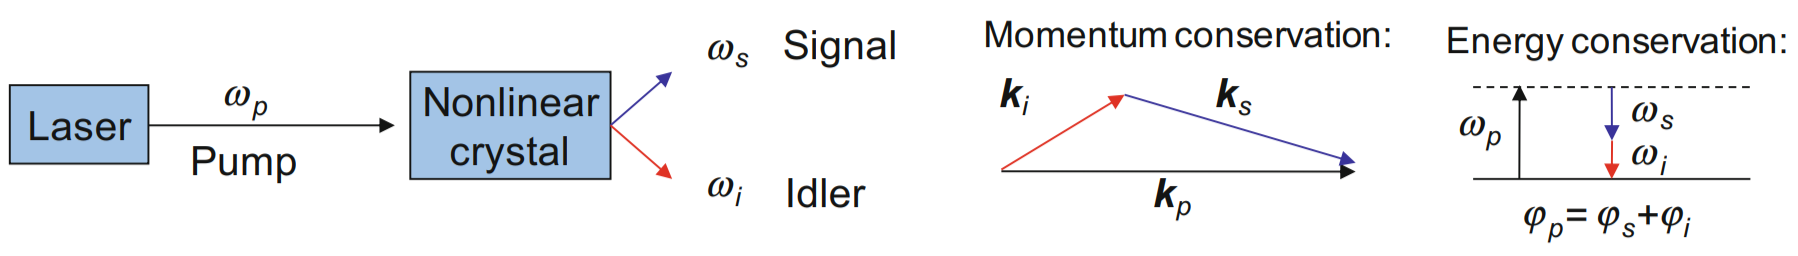
\includegraphics[width=\textwidth]{chapters/figs/fig-7-14}
	\caption{تصویرسازی فرآیند \lr{SPDC}.}
	\label{fig:7-14}
\end{figure}

یک بلور غیرخطی برای تقسیم فوتون‌ها به جفت‌فوتون‌هایی استفاده می‌شود که قانون بقای انرژی را ارضا کرده، مجموع انرژی‌ها و تکانه‌های آن‌ها برابر با انرژی و تکانه فوتون اصلی است، در حوزه فرکانس تطبیق فاز\LTRfootnote{Phase-matched} یافته‌اند و دارای قطبش‌های همبسته هستند. اگر فوتون‌ها دارای قطبش یکسان باشند، به همبستگی نوع \lr{I} تعلق دارند و در غیر این صورت، دارای قطبش‌های عمود بر هم بوده و به نوع \lr{II} تعلق دارند. از آنجا که \lr{SPDC} توسط نوسانات تصادفی خلأ تحریک می‌شود، جفت‌فوتون‌ها در لحظات زمانی تصادفی ایجاد می‌گردند. خروجی یک تبدیل‌کننده پایین‌رتبه نوع \lr{I} به‌عنوان خلأ فشرده\LTRfootnote{Squeezed vacuum} شناخته می‌شود و تنها شامل تعداد فوتون‌های زوج است. خروجی تبدیل‌کننده نوع \lr{II} به‌عنوان حالت خلأ فشرده دو-مُدی\LTRfootnote{Two-mode squeezed vacuum (TMSV)} (\lr{TMSV}) شناخته می‌شود که در ادامه توصیف می‌گردد. متناوباً، فیبر نوری بسیار غیرخطی (\lr{HNLF})\LTRfootnote{Highly nonlinear fiber (HNLF)} نیز می‌تواند به‌عنوان منبع \lr{SPDC} استفاده شود \cite{7-83, 7-84}. \lr{HNLF} از اثر اختلاط چهارموج\LTRfootnote{Four-wave mixing (FWM)} (\lr{FWM}) بهره می‌برد \cite{7-44, 7-85}. هامیلتونی توصیف‌کننده این سیستم شامل جمله دوقطبی $a^\dagger b^\dagger$ خواهد بود. عملگر یکانی گاوسی متناظر، به‌عنوان عملگر فشردگی دو-مُدی\LTRfootnote{Two-mode squeezing operator} شناخته می‌شود:
\begin{equation}
	S_2(s) = \exp\left[ -s(a^\dagger b^\dagger - ab)/2 \right],
	\label{eq:7-94}
\end{equation}
که در آن $s$ میزان فشردگی دو-مُدی را تعیین می‌کند.

در تصویر هایزنبرگ، عملگرهای مربعی $\hat{\bm{x}} = ( \hat{x}_1 \hat{x}_2 \hat{x}_3 \hat{x}_4 )^T = ( \hat{I}_a \hat{Q}_a \hat{I}_b \hat{Q}_b )^T$ به‌صورت زیر تبدیل می‌شوند \cite{7-80}:
\begin{equation}
	\hat{\bm{x}} \rightarrow \bm{\Sigma}_2(s) \hat{\bm{x}}, \quad \bm{\Sigma}_2(s) = \begin{bmatrix} \cosh s \ones & \sinh s \bm{Z} \\ \sinh s \bm{Z} & \cosh s \ones \end{bmatrix},
	\label{eq:7-95}
\end{equation}
که در آن $\ones$ ماتریس همانی و $\bm{Z} = \text{diag}(1, -1)$ ماتریس پاولی-$\bm{Z}$ است. هنگامی که $S_2(s)$ را بر دو حالت خلأ اعمال می‌کنیم، حالت \lr{TMSV} حاصل می‌شود که معمولاً به‌عنوان حالت \lr{EPR} یعنی $\rho_{EPR} = |s\rangle\langle s|_{EPR}$ شناخته می‌شود، که در آن \cite{7-80}:
\begin{equation}
	|s\rangle_{EPR} = \sqrt{1 - \lambda^2} \sum_{n=0}^{\infty} \lambda^n |n\rangle_a |n\rangle_b = \sqrt{\frac{2}{v+1}} \sum_{n=0}^{\infty} \left( \frac{v-1}{v+1} \right)^{n/2} |n\rangle_a |n\rangle_b, \quad \lambda^2 = \frac{v-1}{v+1},
	\label{eq:7-96}
\end{equation}
به‌طوری که $\lambda = \tanh(s)$ و $v = \cosh(2s)$ نشان‌دهنده واریانس مؤلفه‌های مربعی است. حالت \lr{EPR} نشان‌دهنده حالت گاوسی با میانگین صفر و ماتریس کوواریانس زیر است:
\begin{equation}
	\bm{\Sigma}_{EPR} = \begin{bmatrix} v \ones & \sqrt{v^2 - 1} \bm{Z} \\ \sqrt{v^2 - 1} \bm{Z} & v \ones \end{bmatrix}, \quad v = \cosh 2s;
	\label{eq:7-97}
\end{equation}
که در آن عناصر ماتریس کوواریانس با اعمال تعاریف روابط \eqref{eq:7-92} و \eqref{eq:7-93} بر حالت \lr{EPR} تعیین می‌شوند. حالت \lr{EPR} در رابطه \eqref{eq:7-97} مستقیماً در سیستم‌های \lr{CV-QKD} کاربرد دارد.

رایج‌ترین دستگاه‌های مورد استفاده برای دست‌کاری حالت‌های فوتون عبارتند از \cite{7-6, 7-8}: (۱) آینه‌ها، که برای تغییر جهت انتشار استفاده می‌شوند؛ (۲) جابه‌جاگرهای فاز\LTRfootnote{Phase shifters}، که برای اعمال یک جابه‌جایی فاز معین به کار می‌روند؛ و (۳) تقسیم‌کننده‌های پرتو\LTRfootnote{Beam splitters}، که برای پیاده‌سازی گیت‌های مختلف کوانتومی استفاده می‌شوند. جابه‌جاگر فاز قطعه‌ای از یک محیط شفاف، مثلاً شیشه بوروسیلیکات با ضریب شکست $n$ بزرگتر از هوا است و برای انجام عملیات زیر به کار می‌رود:
\begin{equation}
	|\psi_{\text{out}}\rangle = \begin{bmatrix} e^{j\phi} & 0 \\ 0 & 1 \end{bmatrix} |\psi\rangle; \quad \phi = kL, \quad k = n\omega/c.
	\label{eq:7-98}
\end{equation}
طرح معادل متناظر در شکل \ref{fig:7-15} نشان داده شده است.

\begin{figure}[ht]
	\centering
	 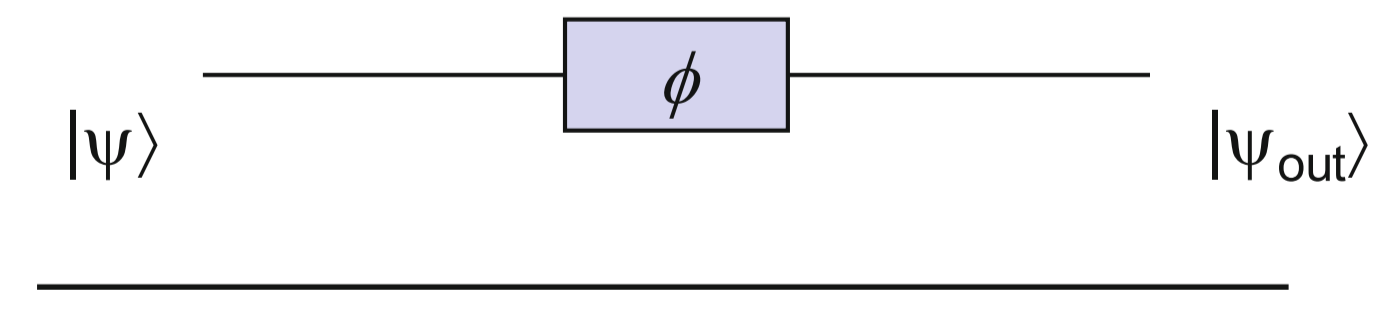
\includegraphics[width=0.5\textwidth]{chapters/figs/fig-7-15}
	\caption{طرح معادل جابه‌جاگر فاز.}
	\label{fig:7-15}
\end{figure}

تقسیم‌کننده پرتو یک قطعه شیشه با پوشش جزئی نقره است که ضریب بازتاب آن به‌صورت $R = \cos \theta$ پارامتری می‌شود. گذردهی\LTRfootnote{Transmissivity} تقسیم‌کننده پرتو به‌صورت $T = \cos^2 \theta \in [0, 1]$ داده می‌شود. در تصویر هایزنبرگ، عملگرهای نابودی مُدها توسط تبدیل بوگولیوبوف زیر تغییر می‌یابند:
\begin{equation}
	\begin{bmatrix} a \\ b \end{bmatrix} \rightarrow \begin{bmatrix} a_{\text{out}} \\ b_{\text{out}} \end{bmatrix} = \begin{bmatrix} \sqrt{T} & \sqrt{1-T} \\ -\sqrt{1-T} & \sqrt{T} \end{bmatrix} \begin{bmatrix} a \\ b \end{bmatrix} = \begin{bmatrix} \cos \theta & \sin \theta \\ -\sin \theta & \cos \theta \end{bmatrix} \begin{bmatrix} a \\ b \end{bmatrix}.
	\label{eq:7-99}
\end{equation}
تقسیم‌کننده پرتو ۵۰:۵۰ به ازای $\theta = \pi/4$ حاصل می‌شود و پیاده‌سازی آن در شکل \ref{fig:7-16} نشان داده شده است.

\begin{figure}[ht]
	\centering
	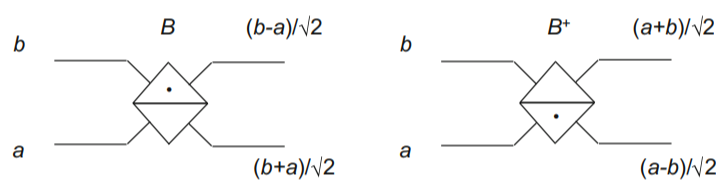
\includegraphics[width=0.7\textwidth]{chapters/figs/fig-7-16}
	\caption{تصویرسازی اصل عملکرد تقسیم‌کننده پرتو ۵۰/۵۰ (\lr{B}) و مزدوج هرمیتی آن ($\bm{B}^\dagger$).}
	\label{fig:7-16}
\end{figure}

تقسیم‌کننده پرتو بر روی دو مُد عمل می‌کند که می‌توان آن‌ها را با عملگرهای تولید (نابودی) $a^\dagger$ ($a$) و $b^\dagger$ ($b$) توصیف کرد. هامیلتونی متناظر به‌صورت زیر داده می‌شود:
\begin{equation}
	\hat{H}_{BS} = j2\theta(a^\dagger b - ab^\dagger).
	\label{eq:7-100}
\end{equation}
عملکرد تقسیم‌کننده پرتو را می‌توان با عملگر تحول به‌صورت زیر نمایش داد:
\begin{equation}
	BS(\theta) = e^{-j\hat{H}_{BS}/2} = e^{\theta(a^\dagger b - ab^\dagger)}.
	\label{eq:7-101}
\end{equation}
عملگرهای مربعی مُدها یعنی $\hat{\bm{x}} = ( \hat{x}_1 \hat{x}_2 \hat{x}_3 \hat{x}_4 )^T = ( \hat{I}_a \hat{Q}_a \hat{I}_b \hat{Q}_b )^T$ توسط تبدیل سیمپلکتیک\LTRfootnote{Symplectic transformation} زیر تغییر می‌یابند:
\begin{equation}
	\hat{\bm{x}} \rightarrow \hat{\bm{x}}_{\text{out}} = \begin{bmatrix} \sqrt{T}\ones & \sqrt{1-T}\ones \\ -\sqrt{1-T}\ones & \sqrt{T}\ones \end{bmatrix} \hat{\bm{x}}.
	\label{eq:7-102}
\end{equation}







\section{پروتکل‌های توزیع کلید کوانتومی با متغیر پیوسته (\lr{CV-QKD})}
\label{sec:7-6}
توزیع کلید کوانتومی با متغیر پیوسته\LTRfootnote{Continuous Variable (CV)-QKD} (\lr{CV-QKD}) را می‌توان با به‌کارگیری آشکارسازی هموداین\LTRfootnote{Homodyne detection}، که در آن در هر لحظه تنها یک مؤلفه مربعی\LTRfootnote{Quadrature component} (به دلیل اصل عدم قطعیت\LTRfootnote{Uncertainty principle}) اندازه‌گیری می‌شود، یا با آشکارسازی هتروداین\LTRfootnote{Heterodyne detection (HD)} (\lr{HD}) پیاده‌سازی کرد؛ در روش دوم، از یک تقسیم‌کننده پرتو\LTRfootnote{Beam splitter (BS)} (\lr{BS}) و دو فتودتکتور متعادل برای اندازه‌گیری هم‌زمان هر دو مؤلفه مربعی استفاده می‌شود، همان‌طور که در شکل \ref{fig:7-17} تصویر شده است.

\begin{figure}[ht]
	\centering
	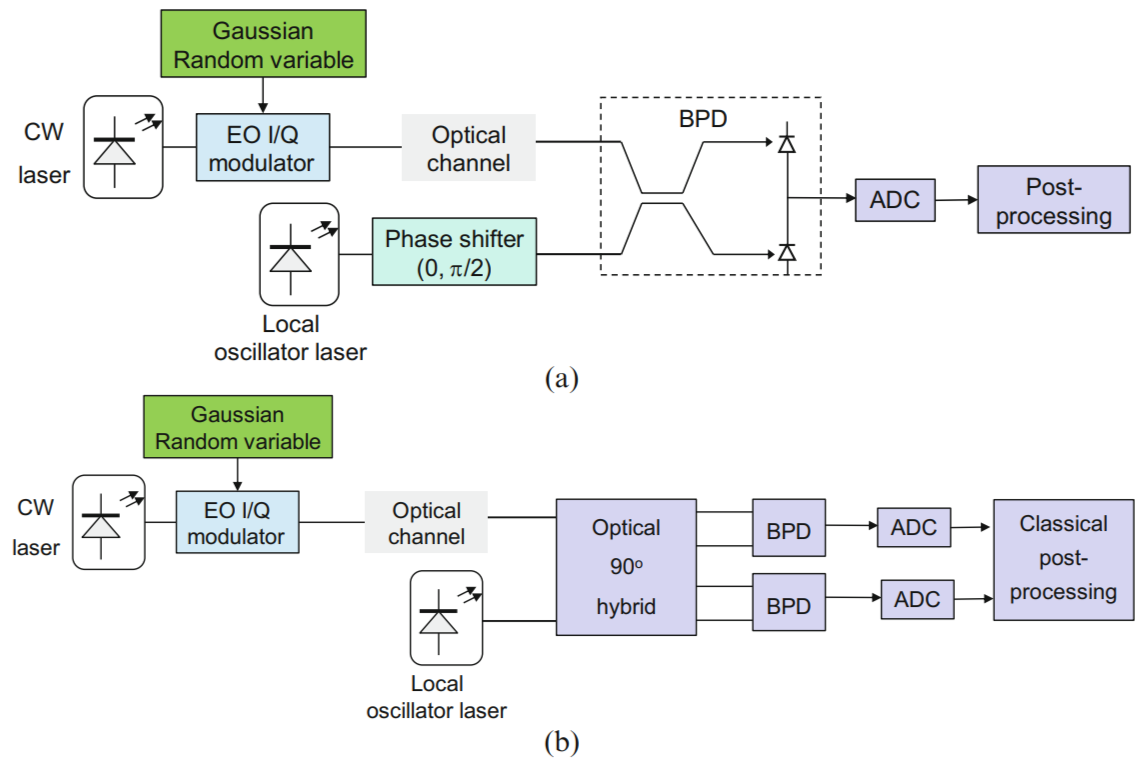
\includegraphics[width=\textwidth]{chapters/figs/fig-7-17}
	\caption{تصویرسازی پروتکل‌های \lr{CV-QKD} مبتنی بر مدولاسیون گاوسی گسسته: (الف) طرح \lr{CV-QKD} مبتنی بر آشکارسازی هموداین؛ (ب) طرح \lr{CV-QKD} مبتنی بر آشکارسازی هتروداین. \lr{ADC}: تبدیل آنالوگ به دیجیتال؛ \lr{BPD}: فتوآشکارسازی متعادل.}
	\label{fig:7-17}
\end{figure}

آشکارسازی هتروداین می‌تواند اطلاعات متقابل\LTRfootnote{Mutual information} بین آلیس و باب را در مقایسه با طرح آشکارسازی هموداین دوبرابر کند، که البته این امر به قیمت تلفات اضافی $3$ \lr{dB} ناشی از تقسیم‌کننده پرتو تمام می‌شود. به‌منظور کاهش نویز فاز لیزر، سیگنال‌های کوانتومی معمولاً همراه با یک تُن پایلوت\LTRfootnote{Pilot-tone (PT)} (\lr{PT}) پرتوانِ تسهیم‌شده در حوزه زمان ارسال می‌شوند تا پایه‌های اندازه‌گیری آلیس و باب با یکدیگر هم‌راستا گردند. برای پیاده‌سازی \lr{CV-QKD}، هم می‌توان از حالت‌های فشرده\LTRfootnote{Squeezed states} و هم از حالت‌های همدوس\LTRfootnote{Coherent states} استفاده کرد. مطالعات \lr{CV-QKD} با قضاوت از روی تعداد فزاینده مقالات مرتبط با این حوزه \cite{7-7, 7-86, 7-87, 7-88, 7-89, 7-90, 7-91, 7-92, 7-93, 7-94, 7-95, 7-96, 7-97, 7-98, 7-99, 7-100, 7-101} و به لطف سازگاری آن‌ها با فناوری‌های پیشرفته مخابرات نوری، در حال شتاب گرفتن است.

سیستم \lr{CV-QKD} هنگام استفاده از مصالحه مستقیم\LTRfootnote{Direct reconciliation}، با محدودیت تلفات $3$ \lr{dB} در گذردهی مواجه می‌شود. برای جلوگیری از این مشکل، یا از روش‌های مصالحه معکوس\LTRfootnote{Reverse reconciliation} \cite{7-86} و یا از روش‌های پس‌گزینش\LTRfootnote{Postselection} \cite{7-96} استفاده می‌شود. استراتژی‌های مختلف شنود که در بخش \ref{sec:7-4-1} بحث شد، برای سیستم‌های \lr{CV-QKD} نیز قابل اعمال هستند. نشان داده شده است که برای مدولاسیون گاوسی\LTRfootnote{Gaussian modulation}، حمله گاوسی بهینه‌ترین حمله برای هر دو نوع حملات انفرادی \cite{7-102} و حملات دسته‌جمعی \cite{7-103, 7-104} است.

\subsection{پروتکل مبتنی بر حالت‌های فشرده}
\label{subsec:7-6-1}
پروتکل‌های مبتنی بر حالت‌های فشرده از اصل عدم قطعیت هایزنبرگ بهره می‌گیرند که بیان می‌کند اندازه‌گیری هر دو مؤلفه مربعی با دقت کامل غیرممکن است. برای اعمال اطلاعات، آلیس به‌طور تصادفی انتخاب می‌کند که از درجه آزادی\LTRfootnote{Degree of freedom (DOF)} (\lr{DOF}) هم‌فاز یا مربعی استفاده کند، همان‌طور که در شکل \ref{fig:7-18} (سمت چپ) نشان داده شده است.

\begin{figure}[ht]
	\centering
	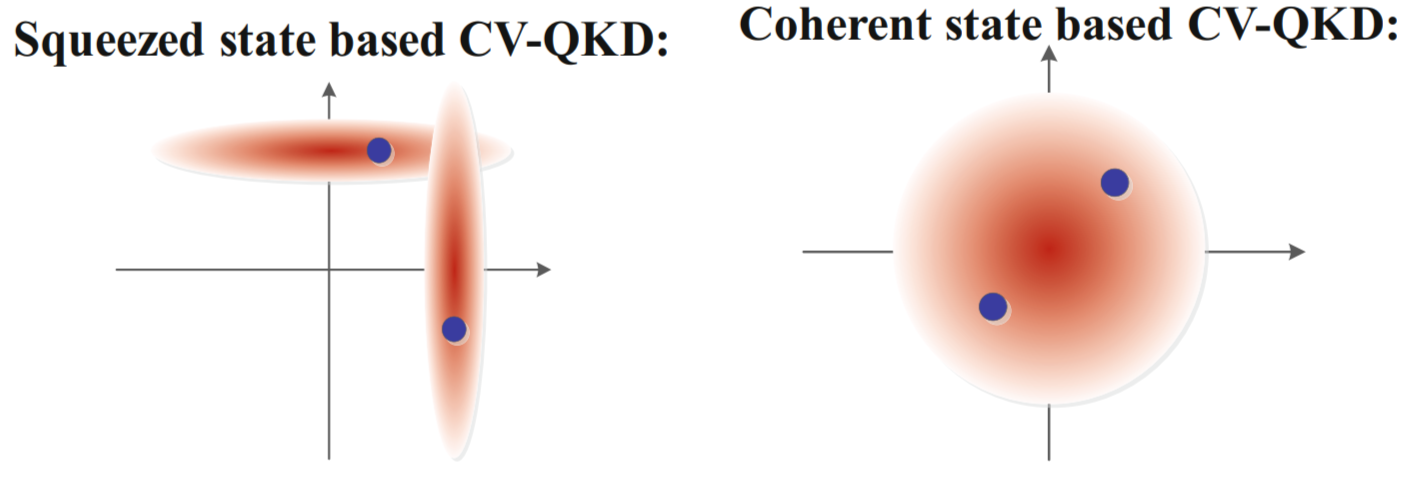
\includegraphics[width=0.9\textwidth]{chapters/figs/fig-7-18}
	\caption{تصویرسازی اصول عملکرد پروتکل‌های مبتنی بر حالت فشرده (چپ) و همدوس (راست).}
	\label{fig:7-18}
\end{figure}

در قاعده کدگذاری آلیس $I$ (زمانی که از \lr{DOF} هم‌فاز استفاده می‌شود)، حالت فشرده بر روی مؤلفه هم‌فاز (با پارامتر فشردگی $s_I < 1$) اعمال می‌شود:
\begin{equation}
	X_{A,I} \rightarrow |X_{A,I}, s_I \rangle, \quad s_I < 1, \quad X_{A,I} \sim \mathcal{N}(0, \sqrt{v_{A,I} N_0})
	\label{eq:7-103}
\end{equation}
دامنه از یک منبع گاوسی با میانگین صفر و واریانس $v_{A,I} N_0$ انتخاب می‌شود. از سوی دیگر، در قاعده کدگذاری آلیس $Q$ (زمانی که از مؤلفه مربعی استفاده می‌شود)، حالت فشرده بر روی مؤلفه مربعی (با پارامتر فشردگی $s_Q > 1$) اعمال شده و می‌توانیم بنویسیم:
\begin{equation}
	X_{A,Q} \rightarrow |jX_{A,Q}, s_Q \rangle, \quad s_Q > 1, \quad X_{A,Q} \sim \mathcal{N}(0, \sqrt{v_{A,Q} N_0})
	\label{eq:7-104}
\end{equation}
واریانس‌های حالت‌های فشرده $I$ و $Q$ به‌ترتیب برابر با $V(\hat{I}) = \sigma_I^2 N_0 = s_I N_0$ و $V(\hat{Q}) = \sigma_Q^2 N_0 = N_0/s_2$ خواهند بود (همان‌طور که در بالا شرح داده شد). در سمت گیرنده، باب به‌طور تصادفی انتخاب می‌کند که مؤلفه $I$ یا $Q$ را اندازه‌گیری کند. آلیس و باب قواعد کدگذاری به‌کار رفته برای اندازه‌گیری مؤلفه مربعی را به ازای هر حالت فشرده مبادله کرده و در فرآیند غربال‌گری، تنها مواردی را که در آن‌ها مؤلفه مربعی یکسانی را اندازه‌گیری کرده‌اند، نگه می‌دارند. بنابراین، این پروتکل بسیار شبیه به پروتکل \lr{BB84} است. سپس مصالحه اطلاعات و به‌دنبال آن تقویت حریم خصوصی انجام می‌شود.

از دیدگاه ایو، حالت‌های مخلوط متناظر زمانی که آلیس از \lr{DOF} هم‌فاز یا مربعی استفاده کرده است، به‌صورت زیر خواهد بود \cite{7-7}:
\begin{equation}
	\begin{aligned}
		\rho_I &= \int f_N(0, \sqrt{v_{A,I} N_0}) |x, s_I \rangle \langle x, s_I| dx, \\
		\rho_Q &= \int f_N(0, \sqrt{v_{A,Q} N_0}) |jQ, s_Q \rangle \langle jQ, s_Q| dx
	\end{aligned}
	\label{eq:7-105}
\end{equation}
که در آن $f_N(0, \sigma)$ توزیع گاوسی با میانگین صفر و واریانس $\sigma^2$ است. هنگامی که شرط $\rho_I = \rho_Q$ برقرار باشد، ایو نمی‌تواند تشخیص دهد که آلیس اطلاعات را روی حالت فشرده $I$ اعمال کرده است یا $Q$. بر اساس رابطه \eqref{eq:7-77}، برای اطمینان از اینکه ایو نتواند بین حالت‌های فشرده $I$ و $Q$ تمایز قائل شود، نیاز داریم که:
\begin{equation}
	(v_{A,I} + \sigma_I^2)\sigma_Q^2 = 1, \quad (v_{A,Q} + \sigma_Q^2)\sigma_I^2 = 1.
	\label{eq:7-106}
\end{equation}
با تقسیم طرفین چپ هر دو معادله، به‌دست می‌آوریم:
\begin{equation}
	\frac{(v_{A,I} + \sigma_I^2)\sigma_Q^2}{(v_{A,Q} + \sigma_Q^2)\sigma_I^2} = 1 \implies 1 + \frac{v_{A,1}}{\sigma_I^2} = 1 + \frac{v_{A,Q}}{\sigma_Q^2}.
	\label{eq:7-107}
\end{equation}
با توجه به اینکه تولید حالت‌های فشرده بسیار دشوارتر از حالت‌های همدوس است، تمرکز خود را بر پروتکل‌های \lr{CV-QKD} مبتنی بر حالت‌های همدوس معطوف می‌کنیم.








\subsection{پروتکل‌های مبتنی بر حالت‌های همدوس}
\label{sec:7-6-2}
در پروتکل‌های مبتنی بر حالت‌های همدوس\LTRfootnote{Coherent states-based protocols}، تنها یک قاعده کدگذاری برای آلیس وجود دارد:
\begin{equation}
	(X_{A,I}, X_{A,Q}) \rightarrow |X_{A,I} + jX_{A,Q} \rangle, \quad X_{A,I} \sim \mathcal{N}(0, \sqrt{v_A N_0}), \quad X_{A,Q} \sim \mathcal{N}(0, \sqrt{v_A N_0})
	\label{eq:7-108}
\end{equation}
به عبارت دیگر، آلیس به‌طور تصادفی نقطه‌ای را در فضای دو‌بعدی (\lr{I, Q}) از یک توزیع گاوسی متقارن دایره‌ای\LTRfootnote{Circular symmetric Gaussian distribution} با میانگین صفر انتخاب می‌کند، همان‌طور که در شکل \ref{fig:7-18} (راست) تصویر شده است. به‌وضوح، هر دو مؤلفه مربعی دارای عدم قطعیت یکسانی هستند. در اینجا نیز مجدداً از اصل عدم قطعیت هایزنبرگ استفاده می‌کنیم که بیان می‌دارد اندازه‌گیری هر دو مؤلفه مربعی با دقت کامل غیرممکن است. در سمت گیرنده، باب اندازه‌گیری تصادفی را روی مؤلفه $I$ یا $Q$ انجام می‌دهد؛ فرض کنید نتیجه اندازه‌گیری او با $Y_B$ نشان داده شود. وقتی باب $I$ را اندازه‌گیری می‌کند، اندازه‌گیری او ($Y_B$) با $X_{A,I}$ همبسته است. از سوی دیگر، وقتی باب $Q$ را اندازه‌گیری می‌کند، نتیجه اندازه‌گیری او ($Y_B$) با $X_{A,Q}$ همبسته است. به‌وضوح، باب قادر است با استفاده از حالت همدوس گاوسی، یک مختصات واحد از نقطه منظومه سیگنال\LTRfootnote{Signal constellation point} ارسال شده توسط آلیس را اندازه‌گیری کند. سپس باب اعلام می‌کند که در هر بازه سیگنال‌دهی کدام مؤلفه مربعی را اندازه‌گیری کرده است و آلیس مختصاتی را انتخاب می‌کند که با مؤلفه مربعی اندازه‌گیری شده توسط باب مطابقت دارد. باقی پروتکل مشابه پروتکل مبتنی بر حالت‌های فشرده است.

از دیدگاه ایو، حالت مخلوط\LTRfootnote{Mixed state} به‌صورت زیر خواهد بود:
\begin{equation}
	\rho = \int f_N(0, \sqrt{v_A N_0}) f_N(0, \sqrt{v_A N_0}) |I + jQ \rangle \langle I + jQ| dI dQ
	\label{eq:7-109}
\end{equation}
در اینجا $v_A$ واریانس مدولاسیون آلیس و $N_0$ نشان‌دهنده واریانس نوسانات حالت‌های همدوس است. برای ارسال بدون تلفات\LTRfootnote{Lossless transmission}، واریانس کل متغیر تصادفی باب به‌صورت زیر خواهد بود:
\begin{equation}
	V(Y_B) = \text{Var}(Y_B) = v_A N_0 + N_0 = (v_A + 1)N_0,
	\label{eq:7-110}
\end{equation}
که از جمله مدولاسیون آلیس $v_A N_0$ و واریانس نوسانات ذاتی حالت همدوس $N_0$ تشکیل شده است.

\subsubsection{مدل کانال همراه با تلفات و اطلاعات متقابل}
\label{subsec:7-6-2-1}
برای ارسال همراه با تلفات\LTRfootnote{Lossy transmission}، کانال را می‌توان به‌صورت یک تقسیم‌کننده پرتو با تضعیف $0 \leq T \leq 1$ مدل‌سازی کرد، همان‌طور که در شکل \ref{fig:7-19} تصویر شده است.

\begin{figure}[ht]
	\centering
	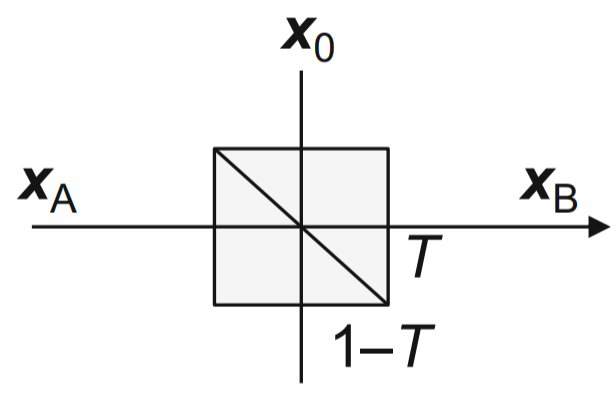
\includegraphics[width=0.8\textwidth]{chapters/figs/fig-7-19}
	\caption{تصویرسازی کانال ارسال همراه با تلفات.}
	\label{fig:7-19}
\end{figure}

از این شکل نتیجه می‌گیریم که حالت خروجی $x_B$ را می‌توان برحسب حالت ورودی $x_A$ و حالت پایه $x_0$ به‌صورت زیر نشان داد:
\begin{equation}
	x_B = \sqrt{T} x_A + \sqrt{1 - T} x_0 = \sqrt{T} (x_A + \sqrt{\chi_{\text{line}}} x_0), \quad \chi_{\text{line}} = (1 - T)/T = 1/T - 1
	\label{eq:7-111}
\end{equation}
برای ارسال همراه با تلفات، زمانی که به جای حالت‌های خلأ از مدولاسیون گاوسی حالت‌های همدوس استفاده می‌شود، رابطه قبلی باید به‌صورت زیر اصلاح گردد:
\begin{equation}
	x_B = \sqrt{T} (x_A + \sqrt{\chi_{\text{line}}} x_0), \quad \chi_{\text{line}} = (1 - T)/T + \epsilon = 1/T - 1 + \epsilon, \quad \epsilon \geq 0
	\label{eq:7-112}
\end{equation}
نخستین جمله در $\chi_{\text{line}}$ مربوط به تضعیف کانال است، در حالی که جمله دوم یعنی $\epsilon$ که معمولاً نویز اضافی\LTRfootnote{Excess noise} نامیده می‌شود، ناشی از سایر عوامل نویزی نظیر نویز فاز لیزر، عدم تعامد کامل مؤلفه‌های مربعی و غیره است. واریانس کل متغیر تصادفی باب اکنون شامل سه جمله خواهد بود:
\begin{equation*}
	V(Y_B) = \text{Var}(Y_B) = T(v_A N_0 + N_0 + \chi_{\text{line}} N_0) = T \left( \underbrace{v_A + 1}_{v} + \chi_{\text{line}} \right) N_0 = T(v + \chi_{\text{line}}) N_0,
\end{equation*}
که در آن $v = v_A + 1$ است.
اطلاعات متقابل بین آلیس و باب بر اساس فرمول شانون\LTRfootnote{Shannon's formula} را می‌توان به‌صورت زیر محاسبه کرد:
\begin{equation}
	I(A; B) \doteq I(X_A; Y_B) = \frac{1}{2} \log \left( 1 + \frac{T v_A N_0}{T(N_0 + \chi_{\text{line}} N_0)} \right) = \frac{1}{2} \log \left( 1 + \frac{v_A}{1 + \chi_{\text{line}}} \right).
	\label{eq:7-113}
\end{equation}
اطلاعات ایو در طرح‌های \lr{CV-QKD} توسط استراتژی مصالحه\LTRfootnote{Reconciliation strategy} تعیین می‌شود.







\subsubsection{مصالحه اطلاعات}
\label{subsec:7-6-3}
در مصالحه مستقیم\LTRfootnote{Direct reconciliation}، کلید بر اساس متغیر تصادفی آلیس $X_A$ تعیین می‌شود (و باب عملیات تصحیح خطا را روی دنباله خود انجام می‌دهد)، به‌طوری که کسر مخفی\LTRfootnote{Secret fraction} به‌صورت زیر داده می‌شود:
\begin{equation}
	r = I(X_A; Y_B) - I(X_A; Z)
	\label{eq:7-114}
\end{equation}
باب و ایو نمی‌توانند هر دو تمام اطلاعات مربوط به عناصر کلیدی پروتکل را به‌دست آورند؛ واریانس باب روی $\hat{I}$ و ایو روی $\hat{Q}$ در رابطه عدم قطعیت $\chi_{\text{line}}\chi_E \geq 1$ صدق می‌کند، به‌طوری که اطلاعات متقابل بین آلیس و ایو به‌صورت زیر به‌دست می‌آید:
\begin{equation}
	I(A; E) = \frac{1}{2} \log \left( 1 + \frac{v_A}{1 + \underbrace{\chi_E}_{1/\chi_{\text{line}}}} \right) = \frac{1}{2} \log \left( 1 + \frac{v_A}{1 + 1/\chi_{\text{line}}} \right).
	\label{eq:7-115}
\end{equation}
با جایگذاری روابط \eqref{eq:7-113} و \eqref{eq:7-115} در \eqref{eq:7-114}، خواهیم داشت:
\begin{equation}
	r = \frac{1}{2} \log \left( 1 + \frac{v_A}{1 + \chi_{\text{line}}} \right) - \frac{1}{2} \log \left( 1 + \frac{v_A}{1 + 1/\chi_{\text{line}}} \right) = \frac{1}{2} \log \left[ \frac{1 + \chi_{\text{line}} + v_A}{1 + \chi_{\text{line}} + v_A \chi_{\text{line}}} \right].
	\label{eq:7-116}
\end{equation}
به ازای $T = 1/2$، مقدار $\chi_{\text{line}} = 1$ شده و آرگومان لگاریتم برابر با $1$ می‌گردد که در نتیجه $r$ صفر می‌شود. بنابراین، در طرح مصالحه مستقیم، تضعیف کانال باید کمتر از $3$ \lr{dB} باشد.

در مصالحه معکوس\LTRfootnote{Reverse reconciliation}، کلید از روی اندازه‌گیری‌های باب تعیین می‌شود (و آلیس تصحیح خطا را روی دنباله خود انجام می‌دهد)، به‌طوری که کسر مخفی به‌صورت زیر است:
\begin{equation}
	r = I(X_B; Y_A) - I(X_B; Z),
	\label{eq:7-117}
\end{equation}
در حالی که اطلاعات متقابل بین باب و آلیس توسط رابطه \eqref{eq:7-113} تعیین می‌شود، اما به شکلی متفاوت بازنویسی می‌گردد:
\begin{equation}
	I(X_B; Y_A) = \frac{1}{2} \log \left( \frac{\overbrace{v_A + 1}^v + \chi_{\text{line}}}{1 + \chi_{\text{line}}} \right) = \frac{1}{2} \log \left( \frac{v + \chi_{\text{line}}}{1 + \chi_{\text{line}}} \right), \quad v = v_A + 1.
	\label{eq:7-118}
\end{equation}
استراتژی شنود گاوسی بهینه بر اساس ماشین کپی‌کننده درهم‌تننده\LTRfootnote{Entangling cloning machine} است که در شکل \ref{fig:7-20} نشان داده شده است.

\begin{figure}[ht]
	\centering
	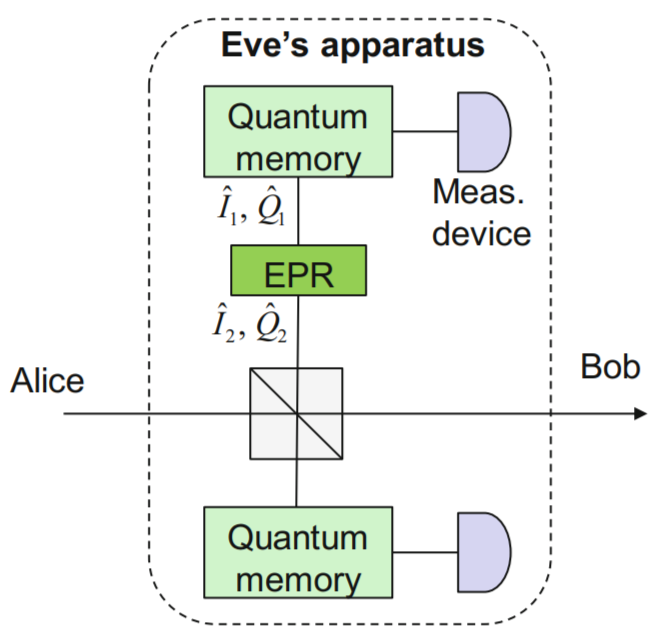
\includegraphics[width=0.6\textwidth]{chapters/figs/fig-7-20}
	\caption{استراتژی شنود گاوسی بهینه بر پایه ماشین کپی‌کننده درهم‌تننده.}
	\label{fig:7-20}
\end{figure}

در دستگاه ایو، از منبع \lr{EPR} استفاده می‌شود که یک نیمه آن توسط ایو در حافظه کوانتومی\LTRfootnote{Quantum memory (QM)} (\lr{QM}) نگه داشته شده و نیمه دیگر توسط یک تقسیم‌کننده پرتو به کانال آلیس-باب تزریق می‌شود. این تقسیم‌کننده پرتو همچنین بخشی از حالت همدوس ارسال شده توسط آلیس را استخراج کرده و ایو آن را در یک \lr{QM} دیگر ذخیره می‌کند تا زمانی که باب اعلام کند در هر بازه سیگنال‌دهی کدام مؤلفه مربعی را اندازه‌گیری کرده است. فرض کنید مؤلفه‌های مربعی بالایی (نگهداری شده توسط ایو در \lr{QM}) با $I_1, Q_1$ و مؤلفه‌های تزریق شده به کانال آلیس-باب با $I_2, Q_2$ نشان داده شوند. به‌وضوح، ایو می‌تواند به‌طور هم‌زمان مؤلفه‌های ارسالی برای باب را با مؤلفه‌های موجود در \lr{QM} خود همبسته کند، چرا که $[I_1 - I_2, Q_1 + Q_2] = 0$ است. از سوی دیگر، با توجه به اینکه $[I_1 - I_2, Q_2] = 2jN_0$ است، همبستگی بین دو مؤلفه هم‌فاز نمی‌تواند کامل باشد و طبق اصل عدم قطعیت داریم $\langle (I_1 - I_2)^2 \rangle \langle Q_2^2 \rangle \geq N_0^2$؛ رابطه مشابهی برای همبستگی‌ها در مؤلفه مربعی $Q$ نیز برقرار است. به‌طور خلاصه، می‌توانیم اصل عدم قطعیت را (در واحد نویز شات\LTRfootnote{Shot noise unit (SNU)}) به‌صورت زیر نمایش دهیم \cite{7-46}:
\begin{equation}
	v_{B|E} v_{B|A} \geq 1,
	\label{eq:7-119}
\end{equation}
که در آن $B$ نماینده هر یک از مؤلفه‌های مربعی باب است.
ما همچنین از تعریف زیر برای واریانس شرطی $v_{X|Y}$ استفاده می‌کنیم که مقدار عدم قطعیت روی $X$ را پس از انجام اندازه‌گیری روی $Y$ کمی‌سازی می‌کند \cite{7-46, 7-105}:
\begin{equation}
	v_{X|Y} = \langle x^2 \rangle - |\langle xy \rangle|^2 / \langle y^2 \rangle.
	\label{eq:7-120}
\end{equation}
آلیس از تخمین‌گرهای $(I_A, Q_A)$ برای میدانی که ارسال می‌کند $(I_A + A_I, Q_A + A_Q)$ استفاده می‌کند، که در آن $\langle A_I^2 \rangle = \langle A_Q^2 \rangle = sN_0$ است و $s > 1/v$ پارامتری است که او برای اطمینان از سازگاری با اصل عدم قطعیت اعمال می‌کند. با محاسبه $\langle Q_A^2 \rangle = (v - s)N_0$، $\langle Q_B^2 \rangle = T(v + \chi_{\text{line}})N_0$ و $\langle Q_A Q_B \rangle = \sqrt{T} \langle Q_A^2 \rangle$ و جایگذاری در رابطه \eqref{eq:7-120}، واریانس شرطی زیر حاصل می‌شود \cite{7-105}:
\begin{equation}
	v_{B|A} = \langle Q_B^2 \rangle - |\langle Q_B Q_A \rangle|^2 / \langle Q_A^2 \rangle = T(s + \chi_{\text{line}})N_0.
	\label{eq:7-121}
\end{equation}
محدودیت $s > 1/v$ رابطه $v_{B|A} \geq T(1/v + \chi_{\text{line}})N_0$ را برای واریانس شرطی به‌دست می‌دهد و از اصل عدم قطعیت \eqref{eq:7-119}، واریانس شرطی زیر برای باب به شرط اندازه‌گیری‌های ایو حاصل می‌شود:
\begin{equation}
	v_{B|E} \geq N_0^2 / [T(1/v + \chi_{\text{line}})N_0].
	\label{eq:7-122}
\end{equation}
اکنون می‌توانیم اطلاعات متقابل بین باب و ایو را به‌صورت زیر محاسبه کنیم \cite{7-105}:
\begin{equation}
	I(B; E) = \frac{1}{2} \log \left( \frac{v_B}{v_{B|E}} \right) = \frac{1}{2} \log \left( \frac{T(v + \chi_{\text{line}})N_0}{\frac{N_0}{T(1/v + \chi_{\text{line}})}} \right) = \frac{1}{2} \log [T^2(v + \chi_{\text{line}})(1/v + \chi_{\text{line}})].
	\label{eq:7-123}
\end{equation}
پس از جایگذاری \eqref{eq:7-118} و \eqref{eq:7-123} در \eqref{eq:7-117}، عبارت کسر مخفی به‌دست می‌آید:
\begin{equation}
	r = I(B; A) - I(B; E) = \frac{1}{2} \log \left( \frac{v + \chi_{\text{line}}}{1 + \chi_{\text{line}}} \right) - \frac{1}{2} \log [T^2 (v + \chi_{\text{line}})(1/v + \chi_{\text{line}})],
	\label{eq:7-124}
\end{equation}
که پس از بازآرایی به‌صورت زیر در می‌آید:
\begin{equation}
	r = -\frac{1}{2} \log [(1 + \chi_{\text{line}}) T^2 (1/v + \chi_{\text{line}})] > 0, \quad T > 0.
	\label{eq:7-125}
\end{equation}
به‌وضوح، تا زمانی که $T > 0$ باشد، کسر مخفی نیز مثبت است.

تا اینجا، ما از آشکارسازی ناقص باب و نویز الکتریکی صرف‌نظر کردیم. با ارجاع به ورودی باب (یا به‌طور معادل خروجی کانال)، می‌توانیم واریانس نویز آشکارساز معادلِ باب را به‌صورت زیر نشان دهیم:
\begin{equation}
	\chi_{\text{det}} = \frac{d(1 + v_{el}) - \eta}{\eta},
	\label{eq:7-126}
\end{equation}
که در آن برای آشکارسازی هموداین $d=1$ و برای آشکارسازی هتروداین $d=2$ است. پارامتر $\eta$ نشان‌دهنده بازدهی آشکارسازی و $v_{el}$ نشان‌دهنده واریانس نویز الکتریکی معادل است. واریانس نویز کل را می‌توان با جمع کردن واریانس نویز کانال و نویز آشکارسازی تعیین کرد، که با ارجاع به ورودی کانال به‌صورت زیر بیان می‌شود:
\begin{equation}
	\chi_{\text{total}} = \chi_{\text{line}} + \frac{\chi_{\text{det}}}{T} = \frac{1 - T}{T} + \epsilon + \frac{d(1 + v_{el}) - \eta}{T\eta}.
	\label{eq:7-127a}
\end{equation}
هنگام ارجاع به خروجی کانال، واریانس نویز کل در سمت باب به‌صورت زیر تعیین می‌شود:
\begin{equation}
	\begin{aligned}
		\chi_{\text{total,Bob}} &= T\eta \left( \chi_{\text{line}} + \frac{\chi_{\text{det}}}{T} \right) = T\eta \frac{1 - T}{T} + T\eta\epsilon + T\eta \frac{d(1 + v_{el}) - \eta}{T\eta} \\
		&= \eta(1 - T) + T\eta\epsilon + d(1 + v_{el}) - \eta.
		\label{eq:7-127b}
	\end{aligned}
\end{equation}
عبارت متناظر برای کسر مخفی \eqref{eq:7-125} باید به‌صورت زیر اصلاح شود:
\begin{equation}
	r = -\frac{1}{2} \log [(1 + \chi_{\text{total}}) (T\eta)^2 (1/v + \chi_{\text{total}})].
	\label{eq:7-128}
\end{equation}









\subsubsection{پیاده‌سازی پروتکل GG02}
\label{subsec:7-6-4}
در این بخش، یک پیکربندی معمول برای سیستم \lr{CV-QKD} \lr{GG02} را شرح می‌دهیم که به نام نویسندگان آن، گروس‌هانز\LTRfootnote{Grosshans} و گرنژیه\LTRfootnote{Grangier} که آن را در سال ۲۰۰۲ پیشنهاد دادند، نام‌گذاری شده است \cite{7-89} (همچنین ببینید \cite{7-7}). طرح متناظر در شکل \ref{fig:7-21} نشان داده شده است.

\begin{figure}[ht]
	\centering
	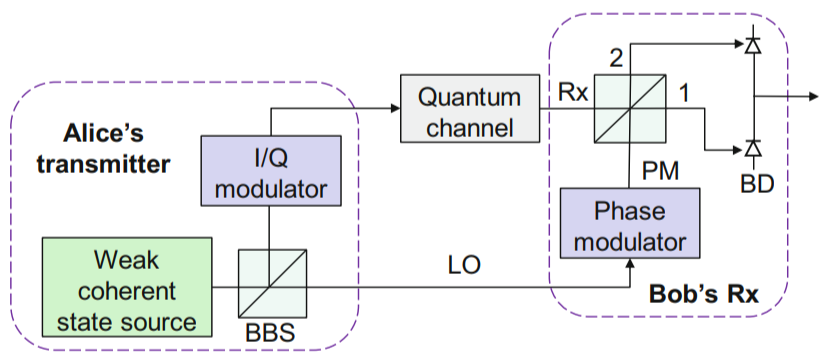
\includegraphics[width=0.8\textwidth]{chapters/figs/fig-7-21}
	\caption{پیکربندی سیستم \lr{CV-QKD} \lr{GG02}. \lr{LO}: سیگنال نوسان‌ساز محلی (مرجع)؛ \lr{BBS}: تقسیم‌کننده پرتو متعادل؛ \lr{BD}: آشکارساز متعادل.}
	\label{fig:7-21}
\end{figure}

آلیس از یک منبع حالت همدوس ضعیف\LTRfootnote{Weak coherent state (WCS)} (\lr{WCS}) مانند باریکه لیزرِ به‌قدر کافی تضعیف‌شده برای به‌دست آوردن حالت گاوسی استفاده می‌کند و در ادامه از یک تقسیم‌کننده پرتو متعادل\LTRfootnote{Balanced beam splitter (BBS)} (\lr{BBS}) برای تقسیم سیگنال به دو بخش بهره می‌برد. خروجی بالایی \lr{BS} توسط مدولاتور \lr{I/Q} مدوله می‌شود تا نقطه منظومه\LTRfootnote{Constellation point} را در مکان مورد نظر در فضای \lr{I-Q} قرار داده و واریانس آلیس $v_A$ را کنترل کند. خروجی دوم \lr{BBS} برای ارسال سیگنال مرجع نوسان‌ساز محلی\LTRfootnote{Local oscillator (LO)} (\lr{LO}) برای باب استفاده می‌شود. تعداد فوتون‌ها در خروجی‌های ۱ و ۲ از \lr{BS} گیرنده را می‌توان به‌صورت زیر بیان کرد:
\begin{equation}
	N_1 = \frac{1}{2} (a_{PM}^\dagger + a_{Rx}^\dagger)(a_{PM} + a_{Rx}), \quad N_2 = \frac{1}{2} (a_{PM}^\dagger - a_{Rx}^\dagger)(a_{PM} - a_{Rx}),
	\label{eq:7-129}
\end{equation}
که در آن عملگرهای تولید (نابودی) در ورودی‌های \lr{Rx} و \lr{PM} از \lr{BS} گیرنده به‌ترتیب با $a_{Rx}^\dagger (a_{Rx})$ و $a_{PM}^\dagger (a_{PM})$ نشان داده شده‌اند. عملگر خروجی آشکارساز متعادل\LTRfootnote{Balanced detector (BD)} (\lr{BD})، با فرض پاسخ‌دهی فتودیود\LTRfootnote{Photodiode responsivity} $P_{\text{ph}} = 1 A/W$، به‌صورت زیر داده می‌شود:
\begin{equation}
	\hat{i}_{BD} = 4N_0 (N_1 - N_2) = 4N_0 (a_{PM}^\dagger a_{Rx} + a_{Rx}^\dagger a_{PM}).
	\label{eq:7-130}
\end{equation}
عملگر نابودیِ خروجی مدولاسیون فاز را می‌توان به‌صورت $a_{PM} = |\alpha| e^{j\theta} \ones / (2\sqrt{N_0})$ نمایش داد و پس از جایگذاری در رابطه (6.162) به‌دست می‌آوریم:
\begin{equation}
	\hat{i}_{BD} = 4N_0 \left( \frac{|\alpha| e^{-j\theta}}{2\sqrt{N_0}} a_{Rx} + \frac{|\alpha| e^{j\theta}}{2\sqrt{N_0}} a_{Rx}^\dagger \right) = 2 |\alpha| \sqrt{N_0} (e^{j\theta} a_{Rx}^\dagger + e^{-j\theta} a_{Rx}).
	\label{eq:7-131}
\end{equation}
در غیاب ایو، عملگر نابودی سیگنال دریافتی به‌صورت $a_{Rx} = (I, Q) \ones / (2\sqrt{N_0})$ خواهد بود که پس از جایگذاری در رابطه (6.163) منجر به نتیجه زیر می‌شود:
\begin{equation}
	\begin{aligned}
		\hat{i}_{BD} &= |\alpha| [ (\cos \theta, \sin \theta) \ones \cdot (\hat{I}, -Q \hat{Q}) + (\cos \theta, \sin \theta) \ones \cdot (\hat{I}, Q \hat{Q}) ] \\
		&= |\alpha| (\cos \theta \cdot I \hat{I} + \sin \theta \cdot Q \hat{Q}).
		\label{eq:7-132}
	\end{aligned}
\end{equation}
باب مؤلفه هم‌فاز $I$ را با انتخاب $\theta = 0$ برای به‌دست آوردن $|\alpha|I$ و مؤلفه مربعی $Q$ را با تنظیم $\theta = \pi/2$ برای به‌دست آوردن $|\alpha|Q$ اندازه‌گیری می‌کند.

واریانس اندازه‌گیری باب دارای مؤلفه‌های زیر است: (۱) واریانس سیگنال، (۲) نوسانات ذاتی $N_0$، (۳) نویز کانال $\chi_{\text{line}} N_0$، (۴) نویز ناشی از آشکارسازی هموداین ناقص $\chi_{\text{homodyne}} N_0 = (1 - \eta)N_0 / \eta$، و (۵) نویز الکترونیکی $v_{el} N_0$؛ بنابراین می‌توانیم بنویسیم:
\begin{equation}
	\chi_{\text{total}} N_0 = \left[ \chi_{\text{line}} + \frac{\chi_{\text{homodyne}} + \overbrace{v_{el}/\eta}^{\chi_{\text{el}}}}{T_{\text{line}}} \right] N_0.
	\label{eq:7-133}
\end{equation}
از روی واریانس‌های سیگنال‌های آلیس و باب $v_A N_0 = \text{Var}(X_A)$ و $\text{Var}(X_B)$ و همچنین ضریب همبستگی $\gamma(X_A, X_B)$، می‌توانیم مقادیر زیر را تعیین کنیم \cite{7-7}:
\begin{equation}
	v_A = \text{Var}(X_A)/N_0, \quad T_{\text{line}} = \gamma^2 \text{Var}(Y_B) / \text{Var}(X_A), \quad \chi_{\text{total}} + 1 = \text{Var}(X_A)(\gamma^{-2} - 1)/N_0.
	\label{eq:7-134}
\end{equation}
اطلاعات متقابل برای کانال آلیس-به-ایو به‌صورت زیر داده می‌شود:
\begin{equation}
	I(A; E) = \frac{1}{2} \log \left( 1 + \frac{v_A}{1 + 1/\chi_{BE}} \right),
	\label{eq:7-135}
\end{equation}
که در اصل همان رابطه \eqref{eq:7-115} است. از سوی دیگر، اطلاعات متقابل برای کانال باب-به-ایو به‌صورت زیر خواهد بود \cite{7-7, 7-106, 7-107}:
\begin{equation}
	I(B; E) = \frac{1}{2} \log \left\{ \frac{T_{\text{line}} T_{\text{extra}} (v + \chi_{\text{total}})}{\chi_{BB} T_{\text{line}} + 1 / [T_{\text{line}} T_{\text{extra}} (1/v + \chi_{BE})]} \right\},
	\label{eq:7-136}
\end{equation}
که نشان‌دهنده تعمیمی از رابطه \eqref{eq:7-123} است. برای یک \textit{رویکرد پارانوئید}\LTRfootnote{Paranoid approach} (زمانی که نویزهای آشکارسازی توسط ایو کنترل می‌شوند)، باید پارامترهای معادلات بالا را به‌صورت زیر تنظیم کنیم \cite{7-7, 7-106, 7-107}:
\begin{equation}
	T_{\text{extra}} = T_{\text{homodyne}}, \quad \chi_{BE} = \chi_{\text{total}}, \quad \chi_{BB} = 0.
	\label{eq:7-137}
\end{equation}
از سوی دیگر، برای یک \textit{رویکرد واقع‌گرایانه}\LTRfootnote{Realistic approach} (زمانی که ایو نمی‌تواند نویزهای آشکارسازی را کنترل کند)، پارامترهای رابطه (6.167) را به‌صورت زیر قرار می‌دهیم \cite{7-7, 7-106, 7-107}:
\begin{equation}
	T_{\text{extra}} = 1, \quad \chi_{BE} = \chi_{\text{line}}, \quad \chi_{BB} = (\chi_{\text{homodyne}} + \chi_{el})/T_{\text{line}}.
	\label{eq:7-138}
\end{equation}
برای مصالحه مستقیم، می‌توانیم کسر مخفی را با $r = I(A; B) - I(A; E)$ محاسبه کنیم. از طرفی، برای مصالحه معکوس، کسر مخفی توسط $r = I(B; A) - I(B; E)$ قابل محاسبه است.









\subsubsection{حملات دسته‌جمعی}
\label{subsec:7-6-5}
در این بخش، به‌اختصار نحوه محاسبه کسر مخفی\LTRfootnote{Secret fraction} برای طرح \lr{CV-QKD} مبتنی بر آشکارسازی هموداینِ حالت همدوس را در شرایطی که ایو از حمله دسته‌جمعی گاوسی\LTRfootnote{Gaussian collective attack} \cite{7-90, 7-103, 7-104} استفاده می‌کند (که به عنوان بهینه‌ترین حالت برای مدولاسیون گاوسی شناخته می‌شود)، شرح می‌دهیم. این حمله به‌طور کامل با تخمین ماتریس کوواریانس\LTRfootnote{Covariance matrix} $\bm{\Sigma}_{AB}$ توسط آلیس و باب مشخص می‌شود که بر اساس رابطه \eqref{eq:7-97} و واریانس مؤلفه هم‌فاز باب که پیش‌تر تعیین شد ($V(\hat{I}) = T\eta(v + \chi_{\text{total}})$)، به‌صورت زیر نمایش می‌یابد:
\begin{equation}
	\bm{\Sigma}_{AB} = \begin{bmatrix} v\ones & \sqrt{T\eta(v^2 - 1)}\bm{Z} \\ \sqrt{T\eta(v^2 - 1)}\bm{Z} & T\eta(v + \chi_{\text{total}})\ones \end{bmatrix}, \quad v = v_A + 1.
	\label{eq:7-139}
\end{equation}
مانند قبل، فرض می‌کنیم $v = v_A + 1$ است که در آن $v_A$ واریانس (نرمالیزه شده) مدولاسیون گاوسی آلیس، $T$ گذردهی کانال، $\eta$ بازدهی آشکارسازی و $\chi_{\text{total}}$ مطابق رابطه \eqref{eq:7-127a} تعریف شده است.

هنگامی که از مصالحه معکوس\LTRfootnote{Reverse reconciliation} استفاده می‌شود، کسر مخفی به‌صورت زیر داده می‌شود:
\begin{equation}
	r = \beta I(A; B) - \chi(B; E),
	\label{eq:7-140}
\end{equation}
که در آن $\beta$ بازدهی مصالحه\LTRfootnote{Reconciliation efficiency} و $I(A; B)$ اطلاعات متقابل بین آلیس و باب است که به همان شیوه حملات انفرادی تعیین می‌شود:
\begin{equation}
	I(A; B) = \frac{d}{2} \log_2 \left( \frac{v + \chi_{\text{total}}}{1 + \chi_{\text{total}}} \right), \quad d = \begin{cases} 1, & \text{آشکارسازی هموداین} \\ 2, & \text{آشکارسازی هتروداین} \end{cases}
	\label{eq:7-141}
\end{equation}
اطلاعات هولِوو\LTRfootnote{Holevo information} بین باب و ایو که با $\chi(B; E)$ نشان داده می‌شود، طبق مراجع \cite{7-90, 7-103, 7-104} به‌صورت زیر تعیین می‌گردد:
\begin{equation}
	\chi(B; E) = g\left(\frac{\lambda_1 - 1}{2}\right) + g\left(\frac{\lambda_2 - 1}{2}\right) - g\left(\frac{\lambda_3 - 1}{2}\right) - g\left(\frac{\lambda_4 - 1}{2}\right),
	\label{eq:7-142}
\end{equation}
که در آن $g(x) = (x + 1)\log_2(x + 1) - x\log_2 x$ آنتروپی یک حالت گرمایی\LTRfootnote{Thermal state} با میانگین تعداد فوتون $x$ است. پارامترهای $\lambda$ طبق مراجع \cite{7-90, 7-108} به‌صورت زیر تعریف می‌شوند:
\begin{equation}
	\begin{aligned}
		\lambda_{1,2} &= \sqrt{\frac{1}{2} (A \pm \sqrt{A^2 - 4B})}, \quad \lambda_{3,4} = \sqrt{\frac{1}{2} (C \pm \sqrt{C^2 - 4D})}, \\
		A &= v^2(1 - 2T) + 2T + T^2(v + \chi_{\text{line}})^2, \quad B = T^2(1 + v\chi_{\text{line}})^2.
	\end{aligned}
	\label{eq:7-143}
\end{equation}
پارامترهای $C$ و $D$ برای آشکارسازی هموداین و هتروداین متفاوت هستند \cite{7-90, 7-108}:
\begin{equation}
	C = \begin{cases} 
		\frac{A\chi_{\text{homodyne}} + v\sqrt{B} + T(v + \chi_{\text{line}})}{T(v + \chi_{\text{total}})}, & \text{آشکارسازی هموداین} \\ 
		\frac{A\chi_{\text{het}}^2 + B + 1 + 2\chi_{\text{het}}[v\sqrt{B} + T(v + \chi_{\text{line}})] + 2T(v^2 - 1)}{T^2(v + \chi_{\text{total}})^2}, & \text{آشکارسازی هتروداین}
	\end{cases}
	\label{eq:7-144}
\end{equation}
\begin{equation}
	D = \begin{cases} 
		\sqrt{B} \frac{v + \chi_{\text{homodyne}}\sqrt{B}}{T(v + \chi_{\text{total}})}, & \text{آشکارسازی هموداین} \\ 
		\left( \frac{v + \chi_{\text{het}}\sqrt{B}}{T(v + \chi_{\text{total}})} \right)^2, & \text{آشکارسازی هتروداین}
	\end{cases}
	\label{eq:7-145}
\end{equation}








\section{پروتکل‌های مستقل از دستگاه اندازه‌گیری (\lr{MDI})}
\label{sec:7-7}
در پروتکل‌های مستقل از دستگاه اندازه‌گیری\LTRfootnote{Measurement-device-independent (MDI) protocols} (\lr{MDI}) \cite{7-109, 7-110, 7-111, 7-112, 7-113}، آلیس و باب از طریق یک کانال کوانتومی (مانند یک پیوند \lr{FSO} یا فیبر نوری) به شخص ثالثی به نام چارلی\LTRfootnote{Charlie} متصل می‌شوند. همان‌طور که در شکل \ref{fig:7-22} برای پیکربندی سیستم \lr{MDI-QKD} تصویر شده است، آشکارسازهای تک-فوتون در سمت چارلی قرار دارند.

\begin{figure}[ht]
	\centering
	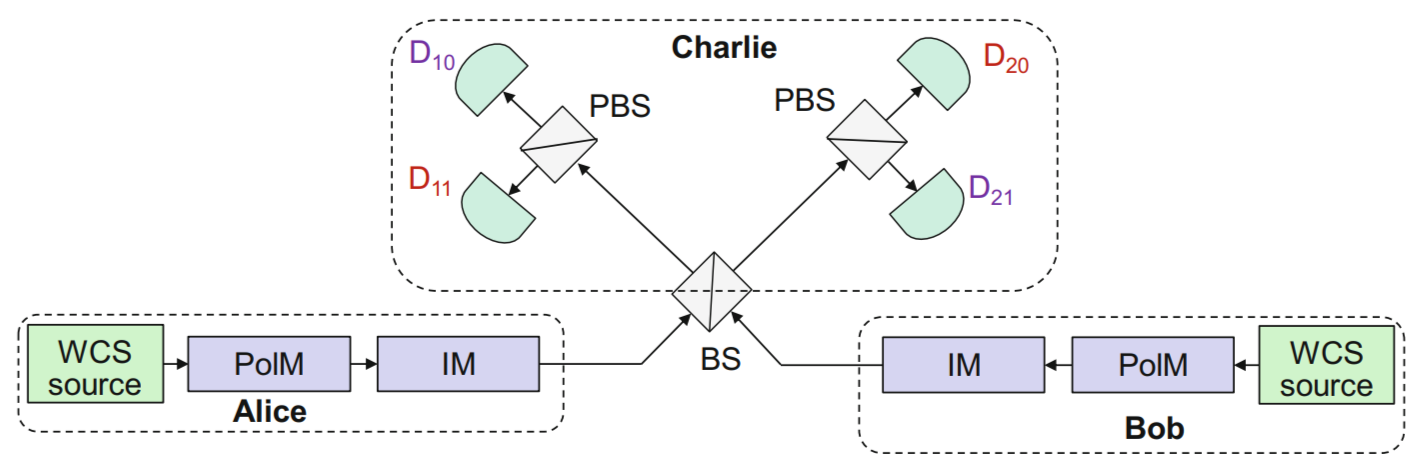
\includegraphics[width=0.8\textwidth]{chapters/figs/fig-7-22}
	\caption{پیکربندی سیستم \lr{MDI-QKD}. \lr{PolM}: مدولاتور قطبش (برای تولید یکی از چهار حالت قطبش $|0\rangle, |1\rangle, |+\rangle, |-\rangle$ استفاده می‌شود)؛ \lr{IM}: مدولاتور شدت (برای تولید حالت‌های سیگنال و فریب با شدت‌های مختلف استفاده می‌شود).}
	\label{fig:7-22}
\end{figure}

نسخه ساده‌شده این پروتکل در ادامه این بخش شرح داده می‌شود. آلیس و باب منابع تک-فوتونی در اختیار دارند و به‌طور تصادفی یکی از چهار حالت $|0\rangle, |1\rangle, |+\rangle, |-\rangle$ را برای ارسال به چارلی انتخاب می‌کنند. چارلی اندازه‌گیری حالت بل\LTRfootnote{Bell state measurement (BSM)} (\lr{BSM}) جزئی را با کمک یک تقسیم‌کننده پرتو انجام داده و رویدادهایی را اعلام می‌کند که در آن‌ها نتیجه اندازه‌گیری منجر به یکی از حالت‌های $|\psi^-\rangle = 2^{-1/2} (|0\rangle_A|1\rangle_B - |1\rangle_A|0\rangle_B)$ یا $|\psi^+\rangle = 2^{-1/2} (|0\rangle_A|1\rangle_B + |1\rangle_A|0\rangle_B)$ شده است. یک \lr{BSM} موفق متناظر با مشاهداتی است که در آن‌ها دقیقاً دو آشکارساز (با قطبش‌های متعامد) به‌صورت زیر تحریک شوند:
\begin{itemize}
	\item کلیک‌های هم‌زمان روی آشکارسازهای $D_{10}$ و $D_{21}$ (یا $D_{11}$ و $D_{20}$)، تصویر شدن بر روی حالت بل $|\psi^-\rangle$ را شناسایی می‌کنند.
	\item از سوی دیگر، کلیک‌ها روی آشکارسازهای $D_{10}$ و $D_{11}$ ($D_{20}$ و $D_{21}$)، تصویر شدن بر روی حالت بل $|\psi^+\rangle$ را شناسایی می‌کنند.
\end{itemize}
سایر الگوهای آشکارسازی موفقیت‌آمیز تلقی نشده و کنار گذاشته می‌شوند.

آلیس و باب سپس در یک کانال کلاسیکِ احرازهویت‌شده و بدون نویز، اطلاعات مربوط به پایه‌های استفاده‌شده را مبادله می‌کنند: پایه $Z$ که توسط حالت‌های $|0\rangle$ و $|1\rangle$ [پایه محاسباتی (\lr{CB})] پوشش داده می‌شود، یا پایه $X$ که توسط حالت‌های $|+\rangle$ و $|-\rangle$ (پایه قطری) پوشش داده می‌شود. آلیس و باب تنها رویدادهایی را نگه می‌دارند که در آن‌ها از پایه یکسانی استفاده کرده‌اند و در همان زمان، چارلی حالت‌های \lr{BSM} یعنی $|\psi^-\rangle$ یا $|\psi^+\rangle$ را اعلام کرده است. یکی از آن‌ها (مثلاً باب) بیت‌های ارسالی را وارونه می‌کند، مگر زمانی که هر دو از پایه قطری استفاده کرده باشند و چارلی حالت $|\psi^+\rangle$ را اعلام کرده باشد. سایر رویدادها دور ریخته می‌شوند.

علاوه بر این، کلید-$X$ از آن بیت‌هایی تشکیل می‌شود که آلیس و باب فوتون‌های خود را در پایه $X$ (پایه قطری) آماده کرده بودند. نرخ خطا در این بیت‌ها برای محدود کردن اطلاعات کسب‌شده توسط ایو استفاده می‌شود. سپس، آلیس و باب کلید-$Z$ را از آن بیت‌هایی تشکیل می‌دهند که برای آن‌ها هر دو از پایه $Z$ (پایه محاسباتی) استفاده کرده‌اند. در نهایت، آن‌ها مصالحه اطلاعات و تقویت حریم خصوصی را روی کلید-$Z$ انجام می‌دهند تا به کلید مخفی دست یابند.

کسر مخفی\LTRfootnote{Secret fraction} پروتکل \lr{MDI-QKD} را می‌توان طبق مرجع \cite{7-112} به‌صورت زیر تخمین زد:
\begin{equation}
	r = q_{11}^{(Z)} [1 - h_2(e_{11}^{(X)})] - q_{\mu\sigma}^{(Z)} f_e h_2(e_{\mu\sigma}^{(Z)}),
	\label{eq:7-146}
\end{equation}
که در آن نمادگذاری‌های زیر معرفی شده‌اند:
\begin{itemize}
	\item $q_{11}^{(Z)}$ نشان‌دهنده احتمالی است که چارلی یک نتیجه موفقیت‌آمیز («بهره»\LTRfootnote{Gain}) را اعلام کند، در حالی که آلیس و باب هر کدام یک تک-فوتون را در پایه $Z$ ارسال کرده‌اند.
	\item $e_{11}^{(X)}$ نشان‌دهنده نرخ خطای فاز سیگنال‌های تک-فوتونی است که هر دو در پایه $Z$ ارسال شده‌اند.
	\item $q_{\mu\sigma}^{(Z)}$ نشان‌دهنده بهره در پایه $Z$ است زمانی که آلیس حالت همدوس ضعیف (\lr{WCS}) با شدت $\mu$ را برای چارلی ارسال کرده، در حالی که باب به‌طور هم‌زمان \lr{WCS} با شدت $\sigma$ را فرستاده است.
\end{itemize}
تابع $h_2(x)$ در معادله فوق نشان‌دهنده تابع آنتروپی باینری است که به‌صورت $h_2(x) = -x \log_2(x) - (1-x) \log_2(1-x)$ تعریف می‌شود.

در معادله بالا، اطلاعات حذف‌شده از کلید نهایی در مرحله تقویت حریم خصوصی توسط جمله $q_{11}^{(Z)} h_2(e_{11}^{(X)})$ توصیف می‌شود. اطلاعات فاش‌شده توسط آلیس در مرحله مصالحه اطلاعات با جمله $q_{\mu\sigma}^{(Z)} f_e h_2(e_{\mu\sigma}^{(Z)})$ توصیف می‌گردد که در آن $f_e$ ناکارآمدی تصحیح خطا\LTRfootnote{Error correction inefficiency} ($f_e \geq 1$) است. نرخ‌های خطای $q_{11}^{(Z)}$ و $e_{11}^{(X)}$ را نمی‌توان به‌طور مستقیم اندازه‌گیری کرد، بلکه در عوض با به‌کارگیری رویکرد حالت فریب محدود می‌شوند.

\section{ملاحظات پایانی}
\label{sec:7-8}
این فصل به مبانی \lr{QKD} اختصاص داشت. فصل با توصیف تفاوت‌های کلیدی بین رمزنگاری متداول، امنیت لایه فیزیکی کلاسیک و \lr{QKD} آغاز شد که در بخش \ref{sec:7-1} شرح داده شدند. در بخش مبانی \lr{QKD} (بخش \ref{sec:7-2})، پس از یک مرور تاریخی، انواع مختلف \lr{QKD} معرفی شدند (بخش \ref{subsec:7-2-1} را ببینید) و توصیف کوتاهی از مراحل معمول پس‌پردازش، مصالحه اطلاعات و تقویت حریم خصوصی در بخش \ref{sec:7-2-2} ارائه گردید. در همان بخش (بخش \ref{subsec:7-2-3})، دو قضیه بنیادی که \lr{QKD} بر آن‌ها استوار است را ارائه دادیم: قضیه کپی‌ناپذیری و قضیه عدم توانایی در تمایز ابهام‌ناپذیر حالت‌های کوانتومی غیرمتعامد. در بخش سیستم‌های \lr{QKD} با متغیر گسسته (\lr{DV}) (بخش \ref{sec:7-3})، پروتکل \lr{BB84} (بخش \ref{subsec:7-3-1}) و پروتکل \lr{B92} (بخش \ref{subsec:7-3-2}) و همچنین پروتکل‌های اکرت (\lr{E91}) و \lr{EPR} (بخش \ref{subsec:7-3-3}) را به‌تفصیل شرح دادیم. در همان بخش، پروتکل کدگذاری فاز-زمان نیز در بخش \ref{subsec:7-3-4} توصیف شده است. در رابطه با پروتکل‌های \lr{BB84}، نسخه‌های مختلف مناسب برای فناوری‌های گوناگون بررسی شدند. در بخش امنیت \lr{QKD} (بخش \ref{sec:7-4})، نرخ کلید مخفی به‌صورت حاصل‌ضرب نرخ کلید خام و نرخ کسری نمایش داده شد و به‌دنبال آن محدودیت‌های مختلف نرخ کلید خام تشریح گردید. سپس، عبارت عمومی برای نرخ کسری ارائه شد و به‌دنبال آن در بخش \ref{sec:7-4-1} انواع استراتژی‌های شنود، شامل حملات انفرادی (مستقل یا غیرهمدوس)، حملات دسته‌جمعی، حملات همدوس و همچنین حملات هک کوانتومی/کانال جانبی توصیف شدند. برای حملات انفرادی و همدوس، عبارات کسر مخفی متناظر شرح داده شد. بخش \ref{sec:7-4-2} به تعاریف مختلف امنیت، از جمله مفهوم $\epsilon$-امنیت اختصاص یافت. سپس، عبارات عمومی برای طرح‌های \lr{DV-QKD} دوبعدی در بخش \ref{subsec:7-4-3} برای هر دو پروتکل آماده‌سازی-و-اندازه‌گیری و پروتکل‌های مبتنی بر حالت فریب استخراج گردید. برای تسهیل توصیف پروتکل‌های \lr{QKD} با متغیر پیوسته (\lr{CV})، ابتدا مبانی اپتیک کوانتومی در بخش \ref{sec:7-5} معرفی شد. در بخش پروتکل‌های \lr{CV-QKD} (بخش \ref{sec:7-6})، هم پروتکل‌های مبتنی بر حالت‌های فشرده (بخش \ref{subsec:7-6-1}) و هم پروتکل‌های مبتنی بر حالت‌های همدوس (بخش \ref{sec:7-6-2}) تشریح شدند. با توجه به اینکه تولید و دست‌کاری حالت‌های همدوس بسیار ساده‌تر است، پروتکل‌های مبتنی بر حالت همدوس با هر دو نوع آشکارسازی هموداین و هتروداین به‌تفصیل در بخش \ref{sec:7-6-2} شرح داده شدند. کسر مخفی برای هر دو پروتکل \lr{CV-QKD} مبتنی بر مصالحه مستقیم و معکوس استخراج گردید. علاوه‌بر این، جزئیات جنبه‌های کاربردی پروتکل \lr{GG02} در بخش \ref{subsec:7-6-4} ارائه شد. در همان بخش، محاسبه کسر مخفی برای حملات دسته‌جمعی در بخش \ref{subsec:7-6-5} مورد بحث قرار گرفت. سپس، مفاهیم پایه برای پروتکل‌های \lr{QKD} مستقل از دستگاه اندازه‌گیری در بخش \ref{sec:7-7} معرفی شدند. برای درک بهتر مبانی \lr{QKD}، مجموعه‌ای از مسائل در بخش بعدی ارائه شده است.











\section{مسائل}
\label{sec:7-9}

\begin{enumerate}
	\item نمودار کسر محرمانگی\LTRfootnote{Secrecy fraction} را برحسب تضعیف\LTRfootnote{Attenuation} برای پروتکل \lr{BB84} رسم کنید. در این مسئله، بازدهی آشکارساز را $0.15$، نرخ شمارش تاریک\LTRfootnote{Dark count rate} را $10^{-6}$، ناکارآمدی مصالحه\LTRfootnote{Reconciliation inefficiency} را $1.1$ و احتمال برخورد فوتون به آشکارساز اشتباه را $0.03$ فرض کنید.
	
	\item برای پروتکل \lr{BB84} مبتنی بر کدگذاری فاز، عبارت مربوط به نرخ کلید مخفی را استخراج کرده و آن را با پروتکل \lr{BB84} متناظر مبتنی بر قطبش مقایسه کنید.
	
	\item مسئله ۱ را برای پروتکل حالت فریب\LTRfootnote{Decoy state protocol} تکرار کرده و درباره بهبودهای حاصل بحث کنید.
	
	\item عبارت نرخ کلید امن را برای پروتکل \lr{B92} استخراج کرده و آن را با پروتکل \lr{BB84} مبتنی بر قطبش مقایسه کنید.
	
	\item عبارت نرخ کلید امن را برای پروتکل اکرت\LTRfootnote{Ekert protocol} استخراج کرده و آن را با پروتکل \lr{BB84} مبتنی بر قطبش مقایسه کنید.
	
	\item نمودار کسر محرمانگی را برحسب تضعیف برای پروتکل \lr{MDI-QKD} با فرض همان پارامترهای سیستم در مسئله ۱ رسم کنید. بهبود حاصل در نرخ کلید مخفی را مورد بحث قرار دهید.
	
	\item با فرض اینکه ایو به‌طور هم‌زمان حملات سد کردن-بازارسال\LTRfootnote{Intercept-resend} و تقسیم تعداد فوتون\LTRfootnote{Photon number splitting} را اعمال می‌کند، عبارت متناظر برای نرخ کلید مخفی بین آلیس و باب را استخراج کنید.
	
	\item استراتژی شنود گاوسی بهینه بر پایه ماشین کپی‌کننده درهم‌تنیده\LTRfootnote{Entangling cloning machine} است که در شکل \ref{fig:7-P7} نشان داده شده است. اطلاعات هولِوو بین باب و ایو را بیابید و نرخ کلید مخفی متناظر را استخراج کنید.
	
	\begin{figure}[H]
		\centering
		\includegraphics[width=0.5\textwidth]{chapters/figs/fig-7-P7}
		\caption{استراتژی شنود گاوسی بهینه بر پایه ماشین کپی‌کننده درهم‌تنیده. \lr{PDs}: فتودتکتورها.}
		\label{fig:7-P7}
	\end{figure}
	
	\item مصالحه اطلاعات معکوس\LTRfootnote{Reverse information reconciliation} را برای کاربردهای \lr{CV-QKD} مبتنی بر کدهای \lr{LDPC} شرح دهید. نحوه تعیین بازدهی مصالحه را توضیح دهید.
	
	\item می‌گوییم کلید نسبت به یک شنودگر $E$ دارای $\epsilon$-امنیت است، اگر فاصله اثر\LTRfootnote{Trace distance} بین حالت مشترک کلید $K$ و ایو $E$ (نشان داده شده با $\rho_{K,E}$) و حالت حاصل‌ضربِ حالت کاملاً مخلوط\LTRfootnote{Completely mixed state (CMS)} (\lr{CMS}) نسبت به مجموعه $K$ تمام کلیدهای امن ممکن (نشان داده شده با $\rho_{CMS}$) و حالت ایو ($\rho_E$)، کوچک‌تر یا مساوی $\epsilon$ باشد. به عبارت دیگر، می‌توانیم بنویسیم:
	\begin{equation}
		D(\rho_{K,E}, \rho_{CMS} \otimes \rho_E) = \frac{1}{2} \|\rho_{K,E} - \rho_{CMS} \otimes \rho_E\|_1 = \frac{1}{2} \text{Tr} |\rho_{K,E} - \rho_{CMS} \otimes \rho_E| \leq \epsilon,
		\label{eq:7-147}
	\end{equation}
	که در آن $|\rho| = \sqrt{\rho^\dagger \rho}$ است. با این تعریف، پارامتر $\epsilon$ تفسیر کاملاً واضحی دارد؛ این پارامتر نشان‌دهنده حداکثر احتمال شکستِ تحمل‌پذیر برای فرآیند استخراج کلید است. با فرض برقرار بودن ویژگی ترکیب‌پذیری\LTRfootnote{Composability} برای این تعریف، می‌توانیم امنیت کلید نهایی $\epsilon$ را برحسب امنیتِ گام‌های تصحیح خطا (\lr{EC}) $\epsilon_{EC}$، تقویت حریم خصوصی (\lr{PA}) $\epsilon_{PA}$ و تخمین پارامتر (\lr{PE}) $\epsilon_{PE}$، و همچنین احتمال شکستِ تخمین‌های آنتروپی رنی (نشان داده شده با $\epsilon_R$) تجزیه کنیم. به عبارت دیگر، می‌توانیم بنویسیم $\epsilon = \epsilon_{EC} + \epsilon_{PA} + \epsilon_{PE} + \epsilon_R$. نامساوی زیر را که نشان‌دهنده تعمیم کران چرنوف\LTRfootnote{Chernoff bound} است، اثبات کنید:
	\begin{equation}
		\text{Pr} \left( D(\rho_{K,E}, \rho_{CMS} \otimes \rho_E) > \epsilon \right) \leq e^{m - f(\rho_{K,E}, \epsilon)},
		\label{eq:7-148}
	\end{equation}
	که در آن $m$ طول کلید مخفی استخراج‌شده است و از ضرایب ثابت صرف‌نظر شده است.
	
	\item یکی از مسائل مهم در \lr{CV-QKD}، زمان مرده\LTRfootnote{Dead time} آشکارسازهای تک‌فوتون\LTRfootnote{Single-photon detectors (SPDs)} (\lr{SPD}) است. بحث کنید که چگونه می‌توان با به‌کارگیری چندین \lr{SPD} بر این مشکل غلبه کرد. عبارت مربوط به نرخ کلید مخفی را به‌عنوان تابعی از تعداد \lr{SPD}ها استخراج کنید.
\end{enumerate}









	% !TeX root = ../quantum.tex

\chapter{توزیع کلید کوانتومی با متغیر گسسته (DV)}
\label{chap:8}

\section*{چکیده}
این فصل به پروتکل‌های توزیع کلید کوانتومی با متغیر گسسته\LTRfootnote{Discrete Variable (DV) QKD} (\lr{DV-QKD}) اختصاص یافته و در واقع ادامه فصل \ref{chap:7} است. فصل با توصیف پروتکل‌های \lr{BB84} و مبتنی بر حالت فریب\LTRfootnote{Decoy state-based protocols} و ارزیابی عملکرد کسر محرمانگی\LTRfootnote{Secrecy fraction} آن‌ها برحسب مسافت دستیابی‌پذیر آغاز می‌شود. موضوع بعدی مربوط به امنیت پروتکل‌های \lr{DV-QKD} در شرایطی است که منابع محدود\LTRfootnote{Finite resources} هستند. ما مفهوم $\epsilon$-امنیت ترکیب‌پذیر\LTRfootnote{Composable $\epsilon$-security} را معرفی کرده و نحوه ارزیابی آن را برای هر دو نوع حملات دسته‌جمعی\LTRfootnote{Collective attacks} و همدوس\LTRfootnote{Coherent attacks} شرح می‌دهیم. همچنین بحث می‌کنیم که چگونه مفاهیم صحت\LTRfootnote{Correctness} و محرمانگی را می‌توان برای دستیابی به کران‌های امنیتی محکم\LTRfootnote{Tight security bounds} ترکیب کرد. پس از آن، پروتکل‌های \lr{BB84} و حالت فریب را تحت فرض کلید محدود بر روی اثرات تلاطم اتمسفری\LTRfootnote{Atmospheric turbulence effects} ارزیابی می‌کنیم. همچنین نحوه مواجهه با شرایط کانال نوری فضای آزاد\LTRfootnote{Free-space optical (FSO) channel} متغیر با زمان را شرح می‌دهیم. سپس تمرکز به سمت پروتکل‌های \lr{QKD} با ابعاد بالا\LTRfootnote{High-dimensional (HD) QKD} (\lr{HD-QKD}) معطوف شده و با توصیف انتخاب پایه‌های متقابلاً بدون سوگیری\LTRfootnote{Mutually unbiased bases (MUBs)} آغاز گشته و با معرفی حالت‌های بل تعمیم‌یافته ادامه می‌یابد. سپس نحوه ارزیابی امنیت پروتکل‌های \lr{HD-QKD} را برای منابع محدود شرح می‌دهیم. در نهایت، انواع پروتکل‌های \lr{HD-QKD} را توصیف می‌کنیم که شامل کدگذاری فاز-زمان\LTRfootnote{Time-phase encoding}، کدگذاری انرژی-زمان\LTRfootnote{Time-energy encoding}، \lr{QKD} ابعاد بالا مبتنی بر \lr{OAM}\LTRfootnote{OAM-based HD QKD}، \lr{QKD} ابعاد بالا مبتنی بر توری‌های براگ فیبری\LTRfootnote{Fiber Bragg grating (FBGs)} (\lr{FBG}) و پروتکل‌های \lr{QKD} ابعاد بالا مبتنی بر توری‌های براگ موجبری\LTRfootnote{Waveguide Bragg gratings (WBGs)} (\lr{WBG}) هستند.







\section{پروتکل‌های BB84 و حالت فریب}
\label{sec:8-1}
در این بخش، پروتکل‌های \lr{BB84} و مبتنی بر حالت فریب را با جزئیات بیشتر شرح داده و عملکرد آن‌ها را مورد بحث قرار می‌دهیم.

\subsection{بازبینی پروتکل BB84}
\label{subsec:8-1-1}
در پروتکل \lr{BB84} \cite{8-1, 8-2, 8-3, 8-4, 8-5}، آلیس به‌طور تصادفی پایه محاسباتی\LTRfootnote{Computational basis} (پایه $Z$) شامل $\{|0\rangle, |1\rangle\}$ یا پایه قطری\LTRfootnote{Diagonal basis} (پایه $X$) شامل $\{|+\rangle, |-\rangle\}$ را انتخاب کرده و متعاقب آن به‌طور تصادفی یکی از حالت‌های پایه را برمی‌گزیند. مقدار منطقی $0$ توسط حالت‌های $|0\rangle$ و $|+\rangle$ و مقدار منطقی $1$ توسط حالت‌های $|1\rangle$ و $|-\rangle$ بازنمایی می‌شود. باب هر کیوبیت\LTRfootnote{Qubit} را با انتخاب تصادفی پایه، اعم از محاسباتی یا قطری، اندازه‌گیری می‌کند. در فرآیند غربال‌گری\LTRfootnote{Sifting procedure}، آلیس و باب پایه‌های استفاده شده برای هر کیوبیت را اعلام کرده و تنها مواردی را که در آن‌ها از پایه یکسانی استفاده کرده‌اند، نگه می‌دارند. از میان بیت‌های باقی‌مانده، آلیس زیرمجموعه‌ای از بیت‌ها را جهت بررسی تداخل ایو\LTRfootnote{Eve} و خطاهای کانال انتخاب کرده و به باب اطلاع می‌دهد که کدام بیت‌ها انتخاب شده‌اند. آلیس و باب مقادیر این بیت‌ها را که برای تخمین نرخ خطای بیت کوانتومی\LTRfootnote{Quantum bit-error rate (QBER)} (\lr{QBER}) استفاده می‌شوند، اعلام و با هم مقایسه می‌کنند. اگر تعداد بیت‌های دارای اختلاف، بیش از مقدار قابل‌قبول (که توسط توانایی تصحیح خطای کد تعیین می‌شود) باشد، آن‌ها پروتکل را متوقف می‌کنند. در غیر این صورت، آلیس و باب مراحل مصالحه اطلاعات\LTRfootnote{Information reconciliation} و تقویت حریم خصوصی\LTRfootnote{Privacy amplification} را روی بیت‌های باقی‌مانده انجام می‌دهند تا بیت‌های کلید مشترک را به‌دست آورند. پیاده‌سازی‌های پروتکل‌های \lr{BB84} متناظر مبتنی بر قطبش و مبتنی بر کدگذاری فاز-زمان پیش‌تر در فصل \ref{chap:6} به همراه نسخه ساده‌شده یعنی پروتکل \lr{B92} \cite{8-6} تشریح شده‌اند. در اینجا به‌اختصار به محاسبه کسر مخفی\LTRfootnote{Secret fraction} در حالت مجانبی\LTRfootnote{Asymptotic case}، یعنی زمانی که اندازه کلید خام به سمت بی‌نهایت میل می‌کند، می‌پردازیم. نرخ کلید مخفی\LTRfootnote{Secret-key rate (SKR)} (\lr{SKR}) متناظر، به‌صورت حاصل‌ضرب کسر مخفی و نرخ کلید خام تعیین می‌شود. عبارت کسر مخفی که از طریق پس‌پردازش یک‌طرفه\LTRfootnote{One-way postprocessing} به‌دست می‌آید، به‌صورت زیر داده می‌شود:
\begin{equation}
	r = I(\bm{A}; \bm{B}) - \min_{\text{\lr{Eve's strategies}}} (I_{EA}, I_{EB}),
	\label{eq:8-1}
\end{equation}
که در آن $I(\bm{A}; \bm{B})$ اطلاعات متقابل\LTRfootnote{Mutual information} بین آلیس و باب است، در حالی که جمله دوم متناظر با اطلاعات ایو $I_E$ درباره کلید خام آلیس یا باب می‌باشد که در آن کمینه‌سازی روی تمام استراتژی‌های شنود ممکن انجام می‌شود.

برای حملات دسته‌جمعی\LTRfootnote{Collective attacks}، اطلاعات ایو درباره دنباله آلیس از طریق اطلاعات هولِوو\LTRfootnote{Holevo information} به‌صورت زیر تعیین می‌شود \cite{8-7, 8-8}:
\begin{equation}
	I_{EA} = \max_{\text{\lr{Eve's strategies}}} \chi(\bm{A}; \bm{E}),
	\label{eq:8-2}
\end{equation}
که در آن بیشینه‌سازی روی تمام استراتژی‌های شنود دسته‌جمعی ممکن انجام می‌شود. تعریف مشابهی برای $I_{BE}$ نیز برقرار است. این کران با نام کران دوتک-وینتر\LTRfootnote{Devetak-Winter bound} نیز شناخته می‌شود. اطلاعات هولِوو که در مرجع \cite{8-9} معرفی شده است، در اینجا به‌صورت زیر تعریف می‌شود:
\begin{equation}
	\chi(\bm{A}; \bm{E}) = S(\rho_E) - \sum_{a} p(a) S(\rho_{E|a}),
	\label{eq:8-3}
\end{equation}
که در آن $S(\rho)$ آنتروپی فون نویمان\LTRfootnote{von Neumann entropy} است که به‌صورت $S(\rho) = -\text{Tr}(\rho \log \rho) = -\sum_i \lambda_i \log \lambda_i$ تعریف می‌شود و در آن $\lambda_i$ مقادیر ویژه عملگر (حالت) چگالی\LTRfootnote{Density operator} $\rho$ هستند. در رابطه \eqref{eq:8-3}، $p(a)$ نشان‌دهنده احتمال وقوع نماد $a$ از الفبای کلاسیک آلیس است، در حالی که $\rho_{E|a}$ عملگر چگالی متناظر با سیستم کمکی\LTRfootnote{Ancilla} ایو است. در نهایت، $\rho_E$ حالت چگالی جزئی ایو است که به‌صورت $\rho_E = \sum_a p(a) \rho_{E|a}$ تعریف می‌شود. به عبارت دیگر، اطلاعات هولِوو متناظر با میانگین کاهش در آنتروپی فون نویمان ایو (عدم قطعیت) است، با این فرض که می‌دانیم $\rho_E$ چگونه آماده‌سازی شده است.

کران پایین کسر مخفی که با پروتکل \lr{BB84} قابل دستیابی است، به‌صورت زیر است:
\begin{equation}
	r = q_1^{(Z)} [1 - h_2(e_1^{(X)})] - q^{(Z)} f_e h_2(e^{(Z)}),
	\label{eq:8-4}
\end{equation}
که در آن $q_1^{(Z)}$ نشان‌دهنده احتمال اعلام یک نتیجه موفقیت‌آمیز (بهره\LTRfootnote{Gain}) در زمانی است که آلیس یک تک‌فوتون ارسال کرده و باب آن را در پایه $Z$ آشکار کرده است، $f_e$ نشان‌دهنده ناکارآمدی تصحیح خطا ($f_e \geq 1$) است، $e^{(X)}$ [$e^{(Z)}$] نشان‌دهنده نرخ \lr{QBER} در پایه $X$ (پایه $Z$) است، و $h_2(x)$ تابع آنتروپی باینری\LTRfootnote{Binary entropy function} است که به‌صورت زیر تعریف می‌شود:
\begin{equation}
	h_2(x) = -x \log_2 x - (1-x) \log_2 (1-x).
	\label{eq:8-5}
\end{equation}
جمله دوم یعنی $q^{(Z)} h_2[e^{(X)}]$ نشان‌دهنده مقدار اطلاعاتی است که ایو توانسته در طول ارسال کلید خام به‌دست آورد و این اطلاعات معمولاً در مرحله تقویت حریم خصوصی از کلید نهایی حذف می‌شود. جمله آخر یعنی $q^{(Z)} f_e h_2[e^{(Z)}]$ نشان‌دهنده مقدار اطلاعات فاش شده در مرحله مصالحه اطلاعات (تصحیح خطا) است که معمولاً به بیت‌های توازن\LTRfootnote{Parity bits} تبادل شده در یک کانال عمومی بدون نویز مربوط می‌شود (زمانی که از تصحیح خطای سیستماتیک استفاده می‌شود).






\subsection{پروتکل‌های حالت فریب}
\label{subsec:8-1-2}
هنگامی که به جای یک منبع تک‌فوتون، از منبع حالت همدوس ضعیف\LTRfootnote{Weak coherent state (WCS)} (\lr{WCS}) استفاده می‌شود، این طرح نسبت به حمله تقسیم تعداد فوتون\LTRfootnote{Photon number splitting (PNS) attack} (\lr{PNS}) حساس خواهد بود؛ موضوعی که در فصل \ref{chap:7} مورد بحث قرار گرفت. با توجه به اینکه اکنون احتمال ارسال چندین فوتون از \lr{WCS} غیر‌صفر است، ایو می‌تواند از این واقعیت برای کسب اطلاعات از کانال بهره‌برداری کند. برای غلبه بر حمله \lr{PNS}، می‌توان از سیستم‌های توزیع کلید کوانتومی مبتنی بر حالت فریب\LTRfootnote{Decoy state} استفاده کرد \cite{8-10, 8-11, 8-12, 8-13, 8-14, 8-15, 8-16, 8-17, 8-18, 8-19, 8-20, 8-21, 8-22}. در \lr{QKD} حالت فریب، میانگین تعداد فوتون‌های ارسالی در بازه‌های زمانی تصادفی افزایش می‌یابد که به آلیس و باب اجازه می‌دهد تشخیص دهند که آیا در زمان ارسال چندین فوتون، ایو در حال سرقت فوتون‌ها است یا خیر. نسخه‌های مختلفی از پروتکل‌های مبتنی بر حالت فریب وجود دارد. در پروتکل مبتنی بر «تک-حالت-فریب»، علاوه بر حالت سیگنال با میانگین تعداد فوتون $\mu$، حالت فریب با میانگین تعداد فوتون $\nu < \mu$ نیز به کار گرفته می‌شود. آلیس ابتدا درباره سطوح میانگین تعداد فوتون سیگنال و فریب تصمیم‌گیری کرده و سپس بر اساس رابطه نرخ کلید مخفی (\lr{SKR})\LTRfootnote{Secret-key rate (SKR)} متناظر، احتمالات بهینه برای استفاده از این دو سطح را تعیین می‌کند. در پروتکل مبتنی بر «حالت فریب ضعیف به‌علاوه خلاء»، علاوه بر سطوح $\mu$ و $\nu$، از حالت خلاء\LTRfootnote{Vacuum state} نیز به‌عنوان حالت فریب استفاده می‌شود. هر دو پروتکل در مرجع \cite{8-19} به‌صورت تئوری و تجربی ارزیابی شده‌اند. نتیجه‌گیری شد که استفاده از یک حالت سیگنال و دو حالت فریب کافی است، که این موضوع با یافته‌های مراجع \cite{8-20, 8-21} مطابقت دارد.

احتمالی که آلیس بتواند فوتون را با موفقیت آشکارسازی کند، زمانی که از \lr{WCS} با میانگین تعداد فوتون $\mu$ استفاده می‌کند، با $q_\mu$ نشان داده می‌شود و به‌عنوان بهره\LTRfootnote{Gain} شناخته می‌شود که می‌تواند توسط رابطه زیر تعیین گردد:
\begin{equation}
	q_\mu = \sum_{n=0}^{\infty} y_n \frac{e^{-\mu} \mu^n}{n!},
	\label{eq:8-6}
\end{equation}
که در آن $y_n$، که به‌عنوان بازده\LTRfootnote{Yield} نیز شناخته می‌شود، احتمال آشکارسازی موفقیت‌آمیز باب در زمانی است که آلیس $n$ فوتون ارسال کرده است. رابطه مشابهی برای حالت‌های فریب با میانگین تعداد فوتون $\sigma_i$ برقرار است، یعنی:
\begin{equation}
	q_{\sigma_i} = \sum_{n=0}^{\infty} y_n \frac{e^{-\sigma_i} \sigma_i^n}{n!}.
	\label{eq:8-7}
\end{equation}
اگر $e_n$ نشان‌دهنده نرخ خطای بیت کوانتومی (\lr{QBER}) متناظر با حالتی باشد که آلیس $n$ فوتون ارسال کرده است، میانگین \lr{QBER} برای حالت همدوس $|\mu \exp(j\phi)\rangle$ (که در آن $\phi$ فاز دلخواه است) را می‌توان به‌صورت زیر تخمین زد:
\begin{equation}
	\bar{e}_\mu = \frac{1}{q_\mu} \sum_{n=0}^{\infty} y_n e_n \frac{e^{-\mu} \mu^n}{n!}.
	\label{eq:8-8}
\end{equation}
اگر $T$ بازدهی کل ارسال\LTRfootnote{Overall transmission efficiency}، متشکل از گذردهی کانال\LTRfootnote{Channel transmissivity} $T_{ch}$، بازدهی فتودتکتور\LTRfootnote{Photodetector efficiency} $\eta$ و گذردهی بخش نوری باب $T_{Bob}$ باشد، بازدهی ارسال پالس $n$-فوتونی به‌صورت زیر خواهد بود:
\begin{equation}
	T_n = 1 - (1 - T)^n.
	\label{eq:8-9}
\end{equation}
در غیاب ایو، برای $n=0$، بازده $y_0$ تحت تأثیر نرخ آشکارسازی پس‌زمینه\LTRfootnote{Background detection rate}، که با $p_d$ نشان داده می‌شود، قرار دارد؛ بنابراین می‌توانیم بنویسیم $y_0 = p_d$. از سوی دیگر، بازده برای $n \geq 1$ توسط هر دو عامل فوتون‌های سیگنال و نرخ پس‌زمینه به‌صورت زیر تعیین می‌شود:
\begin{equation}
	y_n = T_n + y_0 - T_n y_0 = T_n + y_0(1 - T_n) = 1 - (1 - y_0)(1 - T)^n.
	\label{eq:8-10}
\end{equation}
نرخ خطای حالت‌های $n$-فوتونی $e_n$ را می‌توان طبق مراجع \cite{8-10, 8-22} به‌صورت زیر تخمین زد:
\begin{equation}
	e_n = \frac{1}{y_n} (e_0 y_0 + e_d T_n) \cong e_d + \frac{y_0}{y_n} (e_0 - e_d),
	\label{eq:8-11}
\end{equation}
که در آن $e_d$ احتمال برخورد یک فوتون به یک آشکارساز اشتباه است. برای کدگذاری فاز-زمان، این مقدار نشان‌دهنده نرخ خطای عدم‌انطباق ذاتی\LTRfootnote{Intrinsic misalignment error rate} است. در غیاب فوتون‌های سیگنال، با فرض اینکه دو آشکارساز دارای نرخ‌های پس‌زمینه یکسانی هستند، می‌توانیم بنویسیم $e_0 = 1/2$. به‌طور مشابه، میانگین \lr{QBER} را می‌توان به‌صورت زیر تخمین زد:
\begin{equation}
	\bar{e}_\mu = e_d + \frac{y_0}{q_\mu} (e_0 - e_d).
	\label{eq:8-12}
\end{equation}
اکنون می‌توان کران پایین کسر محرمانگی را با اصلاح رابطه مربوط به پروتکل‌های \lr{BB84} به‌صورت زیر تعیین کرد:
\begin{equation}
	r = q_1^{(Z)} [1 - h_2(e_1^{(X)})] - q_\mu^{(Z)} f_e h_2(e_\mu^{(Z)}),
	\label{eq:8-13}
\end{equation}
که در آن از زیرنویس $1$ برای نشان دادن پالس‌های تک‌فوتونی و از زیرنویس $\mu$ برای پالسی با میانگین تعداد فوتون $\mu$ استفاده شده است.

به‌عنوان یک نمونه، شکل \ref{fig:8-1} نتایج کسر محرمانگی را برای پروتکل حالت فریب و پروتکل آماده‌سازی-و-اندازه‌گیری \lr{BB84} مبتنی بر \lr{WCS}، با فرض استفاده از فیبر تک‌مُد استاندارد (\lr{SMF}) با ضریب تضعیف $0.21$ \lr{dB/km} ارائه می‌دهد.

\begin{figure}[ht]
	\centering
	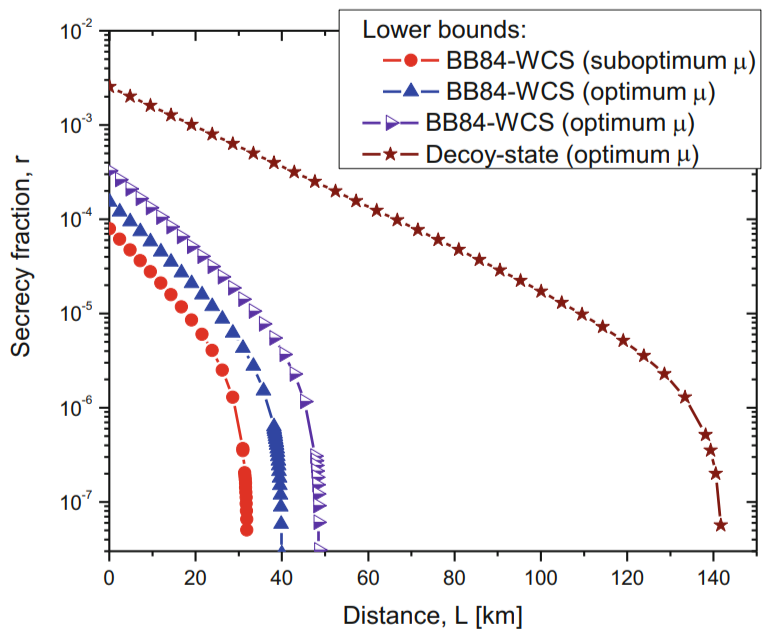
\includegraphics[width=0.8\textwidth]{chapters/figs/fig-8-1}
	\caption{کسر محرمانگی در مقابل مسافت ارسال برای پروتکل مبتنی بر حالت فریب و پروتکل \lr{BB84} مبتنی بر \lr{WCS}.}
	\label{fig:8-1}
\end{figure}






سایر پارامترهای استفاده شده در شبیه‌سازی‌ها به‌صورت زیر تنظیم شده‌اند \cite{8-10, 8-22, 8-23, 8-24}: بازدهی آشکارساز $\eta = 0.045$، نرخ شمارش تاریک $p_d = 1.7 \times 10^{-6}$، احتمال برخورد فوتون به آشکارساز اشتباه $e_d = 0.033$ و ناکارآمدی مصالحه $f_e = 1.22$. برای پروتکل \lr{BB84} مبتنی بر حالت فریب، جهت محاسبه کسر محرمانگی، از رابطه \eqref{eq:8-13} برای مقدار بهینه میانگین تعداد فوتون در هر پالس $\mu$ استفاده می‌کنیم؛ که در آن $q_\mu$ توسط $q_\mu = 1 - (1-y_0)\exp(-\mu T)$ تعیین می‌شود، $e_\mu$ توسط رابطه \eqref{eq:8-12}، $e_1$ توسط رابطه \eqref{eq:8-11} و $q_1$ به‌عنوان آرگومانِ \eqref{eq:8-1} برای $n=1$، یعنی توسط $q_1 = y_1 \mu \exp(-\mu)$ تعیین می‌گردد. برای پروتکل \lr{BB84} مبتنی بر \lr{WCS}، بدون حالت فریب، از رابطه \eqref{eq:8-4} با این فرض استفاده می‌کنیم که ایو کانال را کنترل کرده، حملات سد کردن-بازارسال را انجام می‌دهد و نسبت به حالت‌های چندفوتونی شفاف است. در این سناریوی کران پایین، خطا ناشی از رویدادهای تک‌فوتونی غالب است. اکنون با محاسبه $q^{(Z)}$ توسط $q_\mu = 1 - (1-y_0)\exp(-\mu T)$ و $e^{(Z)}$ توسط $E_\mu = e_d + (e_0 - e_d)y_0 / q_\mu$ و با فرض $\mu$ غیربهینه متناسب با $T$، منحنی قرمز در شکل \ref{fig:8-1} به‌دست آمد که با مرجع \cite{8-10} مطابقت دارد. هنگامی که به جای آن از $\mu$ بهینه (که کسر محرمانگی را بیشینه می‌کند) استفاده می‌کنیم، منحنی آبی به‌دست می‌آید که با مرجع \cite{8-23} مطابقت دارد. برای این دو منحنی، مقدار $q_1^{(Z)}$ را از \eqref{eq:7-6} با قرار دادن $y_n = 1$ برای $n \geq 2$ (ببینید مرجع \cite{8-22}) به‌صورت زیر تخمین می‌زنیم:
\begin{equation}
	q_1^{(X)} \geq q_\mu - \sum_{n=2}^{\infty} \frac{e^{-\mu} \mu^n}{n!}.
	\label{eq:8-14}
\end{equation}
با توجه به اینکه حالت‌های چندفوتونی خطایی ایجاد نمی‌کنند، یعنی برای $n \geq 2$ مقدار $e_n = 0$ است، می‌توانیم $e_1$ را به‌صورت زیر محدود کنیم:
\begin{equation}
	e_1^{(X)} \leq q_\mu E_\mu / q_1^{(X)}.
	\label{eq:8-15}
\end{equation}
رابطه دقیق‌تر برای $q_\mu$ در پروتکل \lr{BB84} مبتنی بر \lr{WCS}، به‌صورت زیر خواهد بود:
\begin{equation}
	q_\mu = y_0 e^{-\mu} + y_1 e^{-\mu} \mu + \sum_{n=2}^{\infty} \frac{e^{-\mu} \mu^n}{n!},
	\label{eq:8-16}
\end{equation}
که از \eqref{eq:7-6} با قرار دادن $y_n = 1$ برای $n \geq 2$ به‌دست می‌آید. منحنی متناظر با رنگ بنفش نشان داده شده است که نشان می‌دهد هنگام استفاده از پروتکل \lr{BB84} مبتنی بر \lr{WCS}، مسافت $L = 48.62$ کیلومتر دستیابی‌پذیر است. در مقابل، برای پروتکل \lr{BB84} مبتنی بر حالت فریب و $\mu$ بهینه، دستیابی به مسافت نزدیک به $141.8$ کیلومتر امکان‌پذیر است که با مرجع \cite{8-23} مطابقت دارد.






\section{امنیت سیستم‌های \lr{QKD} با منابع محدود}
\label{sec:8-2}

همان‌طور که در مرور کلی پروتکل \lr{BB84} بحث شد، پس از اتمام فاز ارسال کلید خام، آلیس و باب فرآیند غربال‌گری\LTRfootnote{Sifting procedure} و تخمین پارامتر\LTRfootnote{Parameter estimation} را انجام می‌دهند، به‌طوری که از $N$ نماد ارسال‌شده، $n$ نماد باقی می‌ماند و کلید متناظر با آن‌ها به‌عنوان کلید غربال‌شده\LTRfootnote{Sifted key} شناخته می‌شود. پس از آن، آن‌ها پس‌پردازش کلاسیک مانند مصالحه اطلاعات\LTRfootnote{Information reconciliation} و تقویت حریم خصوصی\LTRfootnote{Privacy amplification} را انجام می‌دهند. در مرحله مصالحه اطلاعات، آن‌ها از تصحیح خطا\LTRfootnote{Error correction} برای اصلاح خطاهای وارد شده توسط هر دو عاملِ کانال کوانتومی و ایو استفاده می‌کنند و کلید متناظر پس از اتمام این مرحله معمولاً کلید اصلاح‌شده\LTRfootnote{Corrected key} نامیده می‌شود. در طول تقویت حریم خصوصی، آن‌ها همبستگی باقی‌مانده با ایو را حذف می‌کنند و از $n$ نماد، $m$ نماد باقی می‌ماند که کلید متناظر، همان کلید امن\LTRfootnote{Secure key} است. به‌وضوح، نرخ کسریِ کلید مخفی $r$ را می‌توان به‌صورت $r = m/n$ (در حالت $N \to \infty$) تعیین کرد و اغلب از آن به‌عنوان کسر مخفی\LTRfootnote{Secret fraction} یاد می‌شود \cite{8-8}. نرخ کلید مخفی (\lr{SKR})\LTRfootnote{Secret-key rate (SKR)} سپس به‌صورت حاصل‌ضرب کسر مخفی و نرخ کلید خام، که با $R_{\text{raw}}$ نشان داده می‌شود، تعیین می‌گردد و می‌توانیم بنویسیم \cite{8-8}:
\begin{equation}
	\text{SKR} = r \cdot R_{\text{raw}}.
	\label{eq:8-17}
\end{equation}
\lr{QKD} می‌تواند به امنیت غیرمشروط\LTRfootnote{Unconditional security} دست یابد، به این معنی که امنیت آن را می‌توان بدون اعمال هیچ‌گونه محدودیتی بر توان محاسباتی یا استراتژی شنود ایو، تأیید کرد. کران‌های مربوط به نرخ کسر به مراحل پس‌پردازش کلاسیک بستگی دارند. رایج‌ترین روش، پس‌پردازش یک‌طرفه\LTRfootnote{One-way postprocessing} است که در آن آلیس یا باب کلید مرجع\LTRfootnote{Reference key} را در اختیار دارد و اطلاعات کلاسیک را از طریق کانال عمومی برای طرف دیگر ارسال می‌کند، در حالی که طرف مقابل بدون ارائه بازخورد، فرآیند خاصی را روی داده‌ها انجام می‌دهد. مشابه طرح‌های امنیت لایه فیزیکی\LTRfootnote{Physical-layer security (PLS)} (\lr{PLS}) توصیف شده در فصل \ref{chap:4}، معمول‌ترین پردازش یک‌طرفه شامل دو مرحله است: مصالحه اطلاعات و تقویت حریم خصوصی. عبارت کسر مخفی که از طریق پس‌پردازش یک‌طرفه به‌دست می‌آید، بسیار شبیه به طرح‌های \lr{PLS} کلاسیک است \cite{8-8}:
\begin{equation}
	r = I(\bm{A}; \bm{B}) - \min_{\text{\lr{Eve's strategies}}} (I_{EA}, I_{EB}),
	\label{eq:8-18}
\end{equation}
که در آن $I(\bm{A}; \bm{B})$ اطلاعات متقابل بین آلیس و باب است، در حالی که جمله دوم متناظر با اطلاعات ایو $I_E$ درباره کلید خام آلیس یا باب می‌باشد که در آن کمینه‌سازی روی تمام استراتژی‌های شنود ممکن انجام می‌شود. آلیس و باب تصمیم خواهند گرفت که از مصالحه مستقیم یا معکوس استفاده کنند تا بتوانند اطلاعات ایو را کمینه نمایند. در اینجا ما به امنیت در برابر حملات دسته‌جمعی\LTRfootnote{Collective attacks} علاقه‌مند هستیم. در بخش پیش‌ رو، توجه خود را به تعاریف مختلف امنیت معطوف می‌کنیم.





\subsection{نرخ کسر کلید مخفی با طول محدود}
\label{subsec:8-2-1}
فرض کنید کلید ایده‌آل\LTRfootnote{Perfect key} نشان‌دهنده دنباله‌ای از نمادهای کاملاً همبسته بین آلیس و باب باشد که ایو هیچ اطلاعاتی از آن‌ها در اختیار ندارد. کلید $K$ که به اندازه $\epsilon$ از کلید ایده‌آل انحراف داشته باشد، یک کلید $\epsilon$-امن\LTRfootnote{$\epsilon$-secure key} نامیده می‌شود. یکی از الزامات کلیدی که تعریف امنیت باید برآورده کند، ویژگی ترکیب‌پذیری\LTRfootnote{Composability property} است؛ بدین معنا که امنیت کلید صرف‌نظر از نوع کاربرد آن تضمین شده باشد \cite{8-8, 8-25, 8-26, 8-27, 8-28, 8-29}. به عبارت دیگر، اگر کلید $\epsilon$-امن در یک وظیفه $\epsilon'$-امن استفاده شود، کل فرآیند باید حداقل $(\epsilon + \epsilon')$-امن باشد.

\subsubsection{بازبینی $\epsilon$-امنیت مبتنی بر فاصله اثر}
\label{subsec:8-2-1-1}
برای مقابله با این مسئله، بن-اور\LTRfootnote{Ben-Or} و همکاران در \cite{8-25} و همچنین رنر\LTRfootnote{Renner} و کونیگ\LTRfootnote{König} در \cite{8-27} مفهوم $\epsilon$-امنیت مبتنی بر فاصله اثر\LTRfootnote{Trace-distance-based $\epsilon$-security} را معرفی کردند (همچنین ببینید \cite{8-28, 8-30, 8-31, 8-32, 8-33}). می‌گوییم کلید نسبت به شنودگر $E$ دارای $\epsilon$-امنیت است، اگر فاصله اثر بین حالت مشترک کلید $K$ و ایو $E$ (نشان داده شده با $\rho_{K,E}$) و حالت حاصل‌ضربِ حالت کاملاً مخلوط\LTRfootnote{Completely mixed state (CMS)} (\lr{CMS}) نسبت به مجموعه $K$ تمام کلیدهای امن ممکن (نشان داده شده با $\rho_{CMS}$) و حالت ایو (نشان داده شده با $\rho_E$)، کوچک‌تر یا مساوی $\epsilon$ باشد. به عبارت دیگر، می‌توانیم بنویسیم:
\begin{equation}
	D(\rho_{K,E}, \rho_{CMS} \otimes \rho_E) = \frac{1}{2} \|\rho_{K,E} - \rho_{CMS} \otimes \rho_E\|_1 = \frac{1}{2} \text{Tr} |\rho_{K,E} - \rho_{CMS} \otimes \rho_E| \leq \epsilon,
	\label{eq:8-19}
\end{equation}
که در آن $|\rho| = \sqrt{\rho^\dagger \rho}$ است. با این تعریف، پارامتر $\epsilon$ تفسیر کاملاً واضحی دارد؛ این پارامتر نشان‌دهنده حداکثر احتمال شکستِ تحمل‌پذیر برای فرآیند استخراج کلید است. با فرض برقرار بودن ویژگی ترکیب‌پذیری برای این تعریف، می‌توانیم امنیت کلید نهایی $\epsilon$ را برحسب امنیتِ گام‌های تصحیح خطا (\lr{EC})\LTRfootnote{Error correction (EC)} $\epsilon_{EC}$، تقویت حریم خصوصی (\lr{PA})\LTRfootnote{Privacy amplification (PA)} $\epsilon_{PA}$ و تخمین پارامتر (\lr{PE})\LTRfootnote{Parameter estimation (PE)} $\epsilon_{PE}$، و همچنین احتمال شکستِ تخمین‌های آنتروپی رنی\LTRfootnote{Rényi entropy} \cite{8-25} (نشان داده شده با $\epsilon_R$) تجزیه کنیم. به عبارت دیگر، می‌توانیم بنویسیم $\epsilon = \epsilon_{EC} + \epsilon_{PA} + \epsilon_{PE} + \epsilon_R$. کران‌های امنیتی بحث شده در بخش قبلی تنها به‌صورت مجانبی برای کلیدهای بی‌نهایت طولانی، زمانی که $\epsilon \to 0$ است، معتبر هستند. علاوه بر $\epsilon$-امنیت مبتنی بر فاصله اثر، می‌توان از مفهوم $\epsilon$-امنیت مبتنی بر وفاداری\LTRfootnote{Fidelity-based $\epsilon$-security} نیز استفاده کرد \cite{8-25}. با این حال، همان‌طور که در فصل \ref{chap:7} بحث شد، این دو رویکرد با یکدیگر معادل هستند.

اکنون پرسش اصلی این است که چگونه تعریف $\epsilon$-امنیت مبتنی بر فاصله اثر را به طول $m$ کلید مخفی استخراج‌شده مرتبط کنیم. برای این کار، نیاز است نامساوی زیر که نشان‌دهنده تعمیم کران چرنوف\LTRfootnote{Chernoff bound} است، اثبات شود \cite{8-8}:
\begin{equation}
	\text{Pr} \left( D(\rho_{K,E}, \rho_{CMS} \otimes \rho_E) > \epsilon \right) \leq e^{m - f(\rho_{K,E}, \epsilon)},
	\label{eq:8-20}
\end{equation}
که در آن از ضرایب ثابت صرف‌نظر شده است. به‌وضوح، کلید با احتمال بسیار کمی ناامن خواهد بود، به شرطی که شرط زیر برقرار باشد:
\begin{equation}
	m \leq f(\rho_{K,E}, \epsilon).
	\label{eq:8-21}
\end{equation}
به عبارت دیگر، تا زمانی که طول کلید کوتاه‌تر از عدم قطعیت ایو درباره ورودیِ مرحله تقویت حریم خصوصی باشد، کلید امن خواهد بود.

\subsubsection{کمینه-آنتروپی هموار و کسر کلید مخفی با طول محدود تحت حملات دسته‌جمعی}
\label{subsec:8-2-1-2}
آنتروپی رنی از مرتبه $\alpha$ برای متغیر $X$ می‌تواند به‌صورت زیر تعریف شود \cite{8-34}:
\begin{equation}
	R_\alpha(X) = \frac{1}{1 - \alpha} \log_2 \left( \sum_x [P_X(x)]^\alpha \right),
	\label{eq:8-22}
\end{equation}
که در آن $P_X(x)$ توزیع متغیر تصادفی $X$ است. کمینه-آنتروپی\LTRfootnote{Min-entropy} به‌عنوان حالت خاصی از آنتروپی رنی در حد $\alpha \to \infty$ تعریف می‌شود، یعنی:
\begin{equation}
	H_{\min}(X) = H_\infty(X) = \lim_{\alpha \to \infty} R_\alpha(X) = -\log_2 \max_{x \in \mathcal{X}} P_X(x).
	\label{eq:8-23}
\end{equation}
رنر در \cite{8-28} مفهوم کمینه-آنتروپی هموار\LTRfootnote{Smooth min-entropy} را برای پارامتر همواری $\epsilon > 0$ به‌صورت زیر معرفی کرد. فرض کنید $\mathcal{P}(\mathcal{H})$ نشان‌دهنده مجموعه عملگرهای غیرمنفی روی فضای هیلبرت\LTRfootnote{Hilbert space} $\mathcal{H}$ باشد. عملگر چگالی $\rho$ روی $\mathcal{H}$ غیرمنفی است اگر مزدوج هرمیتی با مقادیر ویژه غیرمنفی باشد. همچنین فرض کنید $\rho_{AB} \in \mathcal{P}(\mathcal{H}_A \otimes \mathcal{H}_B)$ و $\sigma_B \in \mathcal{P}(\mathcal{H}_B)$. کمینه-آنتروپی $\rho_{AB}$ نسبت به $\sigma_B$ طبق مرجع \cite{8-28} به‌صورت زیر تعریف می‌شود:
\begin{equation}
	H_{\min}(A|B) \doteq H_{\min}(\rho_{AB} | \sigma_B) = -\log \min \{ \lambda | \lambda \hat{I}_A \otimes \sigma_B - \rho_{AB} \geq 0 \},
	\label{eq:8-24}
\end{equation}
که در آن $\hat{I}_A$ عملگر همانی روی زیرفضای $A$ است. زمانی که $\mathcal{H}_B$ فضای بدیهیِ اعداد مختلط $\mathbb{C}$ باشد، کمینه-آنتروپیِ عملگر چگالی $\rho$ صرفاً به‌صورت زیر است:
\begin{equation}
	H_{\min}(\rho_A) = -\log \lambda_{\max}(\rho).
	\label{eq:8-25}
\end{equation}
کمینه-آنتروپی $\epsilon_R$-هموار برای $\rho_{AB}$ نسبت به $\sigma_B$ به‌صورت زیر تعریف می‌شود \cite{8-28}:
\begin{equation}
	H_{\min}^{\epsilon_R}(\rho_{AB} | \sigma_B) = \sup_{\bar{\rho}_{AB}} H_{\min}(\bar{\rho}_{AB} | \sigma_B),
	\label{eq:8-26}
\end{equation}
که در آن سوپریمم روی تمام عملگرهای $\bar{\rho}_{AB} \in \mathcal{P}(\mathcal{H}_A \otimes \mathcal{H}_B)$ گرفته می‌شود به‌طوری که $\text{Tr}(\bar{\rho}_{AB}) \leq \text{Tr}(\rho_{AB})$ و $\|\bar{\rho}_{AB} - \rho_{AB}\| \leq \epsilon_R \text{Tr}(\rho_{AB})$ باشد. اکنون پروتکل \lr{QKD}ای را در نظر بگیرید که در آن آلیس و باب $N$ جفت درهم‌تنیده را که با $\rho_{A^N B^N}$ نشان داده می‌شوند، به اشتراک می‌گذارند. آلیس و باب سپس اندازه‌گیری را روی کیوبیت‌های متناظر در جفت‌های درهم‌تنیده اعمال می‌کنند. برای اندازه‌گیری‌های فون نویمان\LTRfootnote{von Neumann measurements}، آلیس و باب مالک $N$ بیت با همبستگی بالا خواهند بود. در مرحله تخمین پارامتر، آلیس و باب زیرمجموعه‌ای شامل $p$ جفت همبسته را برای تعیین آمار $\lambda(A,B)$ داده‌های خود انتخاب می‌کنند. در فاز غربال‌گری برخی از جفت‌داده‌ها دور ریخته می‌شوند. برای آلیس و باب به‌ترتیب $n \leq N-p$ بیت باقی می‌ماند که نشان‌دهنده کلید خام است و با $X^n$ و $Y^n$ نشان داده می‌شوند. فرض کنید دنباله بیت‌هایی که ایو موفق به کسب آن‌ها شده است با $E^n$ نشان داده شود. در پس‌پردازش یک‌طرفه، آلیس و باب مراحل بیشتری از مصالحه اطلاعات (تصحیح خطا) و تقویت حریم خصوصی را انجام می‌دهند تا کلید امنی به طول $m \leq n$ به‌دست آورند. کمینه-آنتروپی هموار، تعداد بیت‌های یکنواختی را توصیف می‌کند که می‌توانند در مرحله تقویت حریم خصوصی استخراج شوند \cite{8-28, 8-29}. لم هش باقی‌مانده\LTRfootnote{Leftover hash lemma} از رمزنگاری کلاسیک \cite{8-35, 8-36} به ما می‌گوید که می‌توانیم $m < H_{\min}(X)$ بیت تقریباً به‌طور یکنواخت توزیع‌شده را با تقویت حریم خصوصی از یک متغیر تصارفی $X$ استخراج کنیم. به‌طور دقیق‌تر، برای تابع هشینگ جهانی-$2$ به‌صورت $h(S, X)$، که در آن $S$ روی مجموعه کلیدهای $\mathcal{S}$ یکنواخت است، اگر رابطه زیر برقرار باشد:
\begin{equation}
	m \leq H_{\min}(X) - 2\log \left( \frac{1}{\epsilon_{PA}} \right),
	\label{eq:8-27}
\end{equation}















آنگاه فاصله آماری\LTRfootnote{Statistical distance} محدود می‌شود به:
\begin{equation}
	\delta(h(S,X), (U,S)) \leq \epsilon_{PA},
	\label{eq:8-28}
\end{equation}
که در آن $U$ روی $\{0,1\}^m$ یکنواخت است. فاصله آماری برای دو متغیر تصادفی $\bm{Y}$ و $\bm{Z}$ به‌صورت زیر تعریف می‌شود:
\begin{equation}
	0 \leq \delta(\bm{Y}, \bm{Z}) = \frac{1}{2} \sum_v |Pr(\bm{Y} = v) - Pr(\bm{Z} = v)| \leq 1.
	\label{eq:8-29}
\end{equation}
نامساوی متناظر برای \lr{QKD} صرفاً تعمیمی از \eqref{eq:7-27} به‌صورت زیر خواهد بود:
\begin{equation}
	m \leq H_{\min}^{\epsilon_R}(\bm{X}^n | \bm{E}^n) - 2 \log \left( \frac{1}{\epsilon_{PA}} \right).
	\label{eq:8-30}
\end{equation}
برای استخراج دقیقِ \eqref{eq:8-30}، خواننده علاقه‌مند به مراجع \cite{8-28, 8-37} ارجاع داده می‌شود. فاصله متناظر معادل با \eqref{eq:8-29} به‌صورت زیر داده می‌شود:
\begin{equation}
	\Delta(A|B) = \min_{\sigma_B} \frac{1}{2} \|\rho_{AB} - \hat{I}_A \otimes \sigma_B\|_1, \quad \text{Tr}(\sigma_B) = \text{Tr}(\rho_B), \quad \sigma_B \in \mathcal{P}(\mathcal{H}_B).
	\label{eq:8-31}
\end{equation}
با بازآرایی نامساوی \eqref{eq:8-30}، به‌دست می‌آوریم:
\begin{equation}
	2^{m - H_{\min}^{\epsilon_R}(\bm{X}^n | \bm{E}^n)} \leq 2^{\log \epsilon_{PA}^2},
	\label{eq:8-32}
\end{equation}
که می‌تواند به‌صورت زیر ساده شود:
\begin{equation}
	\sqrt{2^{m - H_{\min}^{\epsilon_R}(\bm{X}^n | \bm{E}^n)}} \leq \epsilon_{PA}.
	\label{eq:8-33}
\end{equation}
اکنون با مقایسه \eqref{eq:8-33} و \eqref{eq:8-28}، نتیجه می‌گیریم که:
\begin{equation}
	\Delta(A|B) = \sqrt{2^{m - H_{\min}^{\epsilon_R}(\bm{X}^n | \bm{E}^n)}} \leq \epsilon_{PA}.
	\label{eq:8-34}
\end{equation}
برای در نظر گرفتن نشت اطلاعات ناشی از تصحیح خطا، باید نامساوی \eqref{eq:8-30} را به‌صورت زیر اصلاح کنیم:
\begin{equation}
	m \leq H_{\min}^{\epsilon_R}(\bm{X}^n | \bm{E}^n) - 2 \log \left( \frac{1}{\epsilon_{PA}} \right) - \text{leakage}_{EC}.
	\label{eq:8-35}
\end{equation}
در پروتکل‌های به کمک درهم‌تنیدگی\LTRfootnote{Entanglement assisted protocols}، آلیس و باب در ابتدا حالت چگالی را به‌صورت $\rho_{A^N B^N} = (\sigma_{AB})^{\otimes N}$ به اشتراک می‌گذارند که در آن $\sigma_{AB}$ یک حالت بل دو-کیوبیتی است. با توجه به اینکه پالایش‌های\LTRfootnote{Purification} مختلف انجام شده توسط ایو تحت تبدیل یکانی محلی\LTRfootnote{Local unitary transformation} معادل هستند، می‌توانیم بنویسیم $\rho_{X^N E^N} = (\sigma_{XE})^{\otimes N}$ به‌طوری که $\sigma_{XE} \in \Gamma$ باشد؛ که در آن $\Gamma$ مجموعه عملگرهای چگالی سازگار با آمار $\lambda(A,B)$ است، به‌جز برای احتمال $\epsilon'_R$. در مراجع \cite{8-28, 8-29, 8-30} نشان داده شده است که کمینه-آنتروپی هموار، برای $\epsilon_R > \epsilon'_R$، از پایین به‌صورت زیر محدود می‌شود:
\begin{equation}
	H_{\min}^{\epsilon_R}(\bm{X}^n | \bm{E}^n) \geq n \left( \min_{\sigma_{XE} \in \Gamma} S(\bm{X}|\bm{E}) - (2D + 3) \sqrt{\frac{\log(2/(\epsilon_R - \epsilon'_R))}{n}} \right),
	\label{eq:8-36}
\end{equation}
که در آن $D$ بعد سیستم و $S(\cdot|\cdot)$ نشان‌دهنده آنتروپی فون نویمان شرطی است.

عبارت متناظر برای کسر کلید مخفی با طول محدود تحت حملات دسته‌جمعی به‌صورت زیر در می‌آید:
\begin{equation}
	r_N = \frac{n}{N} \left[ \min_{\sigma_{XE} \in \Gamma} S(\bm{X}|\bm{E}) - S(\bm{X}|\bm{B}) - \frac{1}{n} \log \left( \frac{2}{\epsilon_{EC}} \right) - \frac{2}{n} \log \left( \frac{1}{\epsilon_{PA}} \right) - (2D + 3) \sqrt{\frac{\log(2/\epsilon_R)}{n}} \right].
	\label{eq:8-37}
\end{equation}
مجموعه حالت‌های $\Gamma$ این واقعیت را در نظر می‌گیرد که تخمین پارامتر\LTRfootnote{Parameter estimation} بر پایه $p$ نمونه استوار است. از قانون اعداد بزرگ\LTRfootnote{Law of large numbers} (قضیه ۱۲.۲.۱ در مرجع \cite{8-38}) می‌دانیم که برای نمونه‌های $X_1, \dots, X_p$ که مستقل و با توزیع یکسان (\lr{i.i.d.}) با توزیع $P(x)$ هستند، رابطه زیر برقرار است:
\begin{equation}
	\text{Pr} \left( \mathcal{D}(P_{x^n} \| P) > \epsilon_{PE} \right) \leq 2^{-p (\epsilon_{PE} - D \ln(p+1)/p)},
	\label{eq:8-38}
\end{equation}
که در آن $\mathcal{D}(\cdot \| \cdot)$ آنتروپی نسبی\LTRfootnote{Relative entropy} است. علاوه‌بر این، از لم ۱۲.۶.۱ در مرجع \cite{8-38} می‌دانیم که برای دو توزیع $P_1$ و $P_2$ رابطه زیر معتبر است:
\begin{equation}
	\mathcal{D}(P_1 \| P_2) \geq \frac{1}{2 \ln 2} \|P_1 - P_2\|_1^2.
	\label{eq:8-39}
\end{equation}
زمانی که آمار $\lambda_p$ با انجام اندازه‌گیری‌های \lr{POVM}\LTRfootnote{POVM measurements} با $D$ نتیجه روی $\sigma$ به‌دست آید، آنگاه برای هر $\epsilon_{PE} > 0$، حالت $\sigma$ در مجموعه زیر قرار خواهد گرفت \cite{8-28, 8-29}:
\begin{equation}
	\Gamma_\xi = \{ \sigma : \|\lambda_p - \lambda_\infty(\sigma)\| \leq \xi \}, \quad \xi = \sqrt{\frac{2 \ln(1/\epsilon_{PA}) + D \ln(p+1)}{p}},
	\label{eq:8-40}
\end{equation}
که در آن $\lambda_\infty(\sigma)$ توزیع احتمال مبتنی بر \lr{POVM} است.





\subsubsection{کسر کلید مخفی با طول محدود تحت حملات همدوس}
\label{subsec:8-2-1-3}
رابطه \eqref{eq:8-37} برای حملات دسته‌جمعی معتبر است، اما همان‌طور که در مرجع \cite{8-30} بحث شده است، می‌توان آن را به حملات همدوس\LTRfootnote{Coherent attacks} نیز تعمیم داد. فرض کنید $\epsilon_{\text{coh}}$ نشان‌دهنده حداکثر احتمال شکستِ تحمل‌پذیر تحت حملات همدوس باشد. با وارد کردن جایگذاری زیر \cite{8-30}:
\begin{equation}
	\epsilon = \epsilon_{\text{coh}} (N + 1)^{-(D^4 - 1)},
	\label{eq:8-41}
\end{equation}
نرخ کسر محرمانگی متناظر برای حملات همدوس به‌صورت زیر در می‌آید \cite{8-30}:
\begin{equation}
	r_{N,\text{coh}} = r_N - \frac{2(D^4 - 1) \log(N + 1)}{N}.
	\label{eq:8-42}
\end{equation}
رویکرد دیگر برای نرخ‌های مخفی با کلید محدود، به‌کارگیری قضیه بازنمایی دِ فینتی\LTRfootnote{de Finetti representation theorem} است \cite{8-28, 8-30, 8-39}. قضیه بازنمایی دِ فینتی، فاصله بین حالت $n$-قسمتی اصلی $\rho_{AB}$ و مخلوطی از حالت‌های حاصل‌ضرب\LTRfootnote{Mixture of product states} $\rho_{A^N B^N} = (\sigma_{AB})^{\otimes N}$ را محدود می‌کند؛ این حالت‌ها معمولاً زمانی به‌دست می‌آیند که حمله دسته‌جمعی توسط ایو اعمال شود \cite{8-28, 8-30, 8-39} و با نام حالت‌های فینتی-هیلبرت-اشمیت\LTRfootnote{Finetti-Hilbert-Schmidt states} شناخته می‌شوند. این قضیه زمانی که کسی بخواهد پروتکل‌های مختلف \lr{QKD} را در سطح حالت‌های کوانتومی مقایسه کند، بسیار دقیق (\textit{Tight}) است. با این حال، همان‌طور که در مرجع \cite{8-30} نشان داده شده است، نتایج نسبتاً بدبینانه‌ای برای نرخ‌های کلید مخفی با طول محدود ارائه می‌دهد. در مرجع \cite{8-40} نشان داده شده است که برای اهداف \lr{QKD} و برخی دیگر از کاربردهای پردازش اطلاعات کوانتومی، مطالعه فاصله بین دو نگاشت ناوردا نسبت به جایگشت\LTRfootnote{Permutation invariant maps} که پروتکل \lr{QKD} را پیاده‌سازی می‌کنند، کافی است. فرض کنیم $p$ بیت از $N_s < N$ بیت غربال‌شده برای تخمین پارامتر استفاده شوند و اثر جزئی $k$ سیستم گرفته شود تا برای ارضای شرایط قضیه دِ فینتی، به حالت حاصل‌ضرب نزدیک شویم. $n = N_s - p - k$ بیت باقی‌مانده نشان‌دهنده کلید خام هستند. فرض کنید $\rho_{| \theta \rangle^n}$ نشان‌دهنده خروجی ناوردا نسبت به دورانِ یک پروتکل \lr{QKD} باشد که به‌طور کلی (برای هر $| \theta \rangle$) به‌صورت حاصل‌ضرب نیست. این حالت را می‌توان در زیرفضای متقارن (ناوردا نسبت به جایگشت) از $\mathcal{H}^n$ به‌صورت $\rho_{| \theta \rangle^n} = \sum \pi | \theta \rangle^{\otimes (n-t)} \otimes | \phi \rangle^{\otimes t}$ نمایش داد، که در آن مجموع روی تمام جایگشت‌های ممکن $\pi$ است و $0 \leq t \leq p/2$ می‌باشد. پارامتر $t$ با فاصله بین $\rho_{| \theta \rangle^n}$ و حالت حاصل‌ضرب $n$-تایی خالص کامل مرتبط است و می‌تواند طبق مراجع \cite{8-28, 8-30} به‌صورت $t = (N_s/k)[2 \ln (2/\epsilon_{\text{deF}}) + D^4 \ln k]$ تعیین شود که در آن $\epsilon_{\text{deF}}$ خطای پارامتری‌کننده $t$ است. خطای کل برای حمله همدوس را اکنون می‌توان به‌صورت $\epsilon = \epsilon_{EC} + \epsilon_{PA} + \epsilon_R + \epsilon_{PE} + \epsilon_{\text{deF}}$ تجزیه کرد. حداکثر خطای تخمین پارامتر برای $p$ نمونه به‌صورت زیر در می‌آید \cite{8-30}:
\begin{equation}
	\xi(p) = \frac{1}{D - 1} \sqrt{\frac{2 \ln(1/\epsilon_{PA}) + D \ln(p + 1)}{p} + (1 + \ln 2) h_2(t/p)},
	\label{eq:8-43}
\end{equation}
که در آن پارامتر $k$ به‌صورت بهینه تعیین شده و $h_2(\cdot)$ تابع آنتروپی باینری است. عبارت متناظر برای نرخ کسر مخفی با طول محدود، برای قضیه دِ فینتی، تحت حملات همدوس به‌صورت زیر در می‌آید \cite{8-28, 8-30}:
\begin{equation}
	r_N = \frac{n}{N} \left[ \min_{\sigma_{XE} \in \Gamma} S(\bm{X}|\bm{E}) - S(\bm{X}|\bm{B}) - \frac{1}{n} \log \frac{2}{\epsilon_{EC}} - \frac{2}{n} \log \frac{1}{\epsilon_{PA}} - \frac{4}{n} (p+k) \log D - \frac{(\frac{5}{2}D + 4) \log(2/\epsilon_R)}{n} + h_2\left(\frac{t}{n}\right) \right].
	\label{eq:8-44}
\end{equation}
با این حال، همان‌طور که در مرجع \cite{8-30} نشان داده شده است، این نرخ کسر مخفی با طول محدود منجر به مقادیر بسیار بدبینانه‌ای برای \lr{SKR} می‌شود.

\subsection{تحلیل دقیق کلید محدود}
\label{sec:8-2-2}
نویسندگان در مرجع \cite{8-41} تعاریف امنیتی را برای در بر گرفتن هر دو مورد صحت\LTRfootnote{Correctness} کلید و $\epsilon$-محرمانگی\LTRfootnote{$\epsilon$-secrecy} (همان‌طور که توسط رنر معرفی شد \cite{8-28}) بسط دادند. پروتکل \lr{QKD} کلید $K$ را در سمت آلیس و کلید $K'$ را در سمت باب خروجی می‌دهد که هر دو دارای طول یکسانی، مثلاً $l$، هستند. می‌گوییم کلید \textit{صحیح} است اگر برای هر استراتژی که ایو اعمال می‌کند، آن‌ها همچنان به کلید یکسانی برسند، یعنی $K' = K$. می‌گوییم پروتکل \lr{QKD} دارای $\epsilon_c$-صحت است اگر $Pr[K' \neq K] \leq \epsilon_c$ باشد. از سوی دیگر، تعریف امنیت، تعمیمی از تعریف ارائه‌شده در رابطه \eqref{eq:8-19} است. می‌گوییم پروتکل $\epsilon_s$-محرمانه است اگر نسبت به پروتکل کاملاً محرمانه، $\epsilon_s$-تمایزناپذیر\LTRfootnote{$\epsilon_s$-indistinguishable} باشد. شرط $\epsilon_s$-محرمانگی را می‌توان به‌صورت زیر فرمول‌بندی کرد:
\begin{equation}
	\min_{\rho_E} (1 - p_{\text{abort}}) D(\rho_{K,E}, \rho_{CMS} \otimes \rho_E) = \frac{1 - p_{\text{abort}}}{2} \min_{\rho_E} \text{Tr} |\rho_{K,E} - \rho_{CMS} \otimes \rho_E| \leq \epsilon_s,
	\label{eq:8-45}
\end{equation}
که در آن $p_{\text{abort}}$ احتمال توقف\LTRfootnote{Abort} پروتکل است. پروتکلی که برای آن $0 = \epsilon_s$ باشد، در اینجا \textit{کاملاً محرمانه} نامیده می‌شود. می‌گوییم پروتکل \textit{امن} است اگر به‌طور هم‌زمان صحیح و محرمانه باشد. به بیان دقیق‌تر، می‌گوییم پروتکل $\epsilon$-امن است، اگر به‌طور هم‌زمان $\epsilon_c$-صحیح و $\epsilon_s$-محرمانه باشد، به‌طوری که $\epsilon_c + \epsilon_s \leq \epsilon$. در نهایت، می‌گوییم پروتکل \textit{صلب}\LTRfootnote{Robust} است اگر در غیاب ایو، با احتمال $\epsilon_r$ متوقف شود. به‌عنوان یک مثال توصیفی، یک پروتکل بدیهی که همیشه متوقف می‌شود امن است، اما منجر به هیچ کلید امنی نمی‌شود. پروتکل $\epsilon$-امن منجر به یک کلید امن به طول $l$ می‌شود. برای در نظر گرفتن صلبیت پروتکل، نرخ کسر محرمانگی با کلید محدود را به‌صورت زیر تعریف می‌کنیم \cite{8-41}:
\begin{equation}
	r = (1 - \epsilon_r) \frac{l}{N(n, p)},
	\label{eq:8-46}
\end{equation}
که در آن $N(n, p)$ نشان‌دهنده تعداد کیوبیت‌هایی است که باید ارسال شوند تا $n$ بیت کلید خام و $p$ بیت برای استفاده در تخمین پارامتر جمع‌آوری گردند. با استفاده از این مفهوم، برای منبع کوانتومی با کیفیت آماده‌سازی $q$، کلید $\epsilon$-امن است اگر نامساوی زیر برقرار باشد:
\begin{equation}
	l \leq n [1 - h_2(Q + \Delta Q)] - \text{leak}_{EC} - \log_2 \left( \frac{2}{\epsilon_s^2 \epsilon_c} \right), \quad \Delta Q = \sqrt{\frac{n + p}{np} \frac{p + 1}{p} \ln \left( \frac{2}{\epsilon_s} \right)},
	\label{eq:8-47}
\end{equation}
که در آن $Q$ حداکثر \lr{QBER} تحمل‌پذیر است و $\Delta Q$ متناظر با اصلاحی است که برای در نظر گرفتن نوسانات آماری اضافه می‌شود. بدیهی است که این تخمین دقیقِ طول کلید محدود برای پروتکل‌های دو‌بعدی قابل اعمال است. با این حال، می‌توان آن را مستقیماً به پروتکل‌های $D$-بعدیِ دو-پایه‌ای تعمیم داد. نشان داده شده است که نرخ‌های کسر محرمانگی متناظر برای $N$ به اندازه کافی بزرگ، با عبارات مبتنی بر تعریف رنر به‌خوبی مطابقت دارند، اما نتایج عددی نشان می‌دهند که نرخ‌های محرمانگی واقعی برای طول‌های کلید غربال‌شده‌ی $N$ کم و متوسط، بسیار بالاتر از مقادیر پیش‌بینی شده توسط تئوری رنر هستند.

\section{تحلیل کلید محدود برای پروتکل‌های QKD BB84 و حالت فریب روی کانال‌های تلاطم اتمسفری}
\label{sec:8-3}
در این بخش، تحلیل کلید محدود نرخ‌های کسر امن را برای پروتکل‌های \lr{BB84} مبتنی بر حالت همدوس ضعیف (\lr{WCS}) و حالت فریب در حضور اثرات تلاطم اتمسفری ارائه می‌دهیم \cite{8-21}. (توجه داشته باشید که در اینجا از نمادگذاری هماهنگ با این فصل استفاده می‌کنیم، نه نمادگذاری مرجع \cite{8-21}).





\subsection{پروتکل BB84 روی کانال‌های FSO متغیر با زمان}
\label{subsec:8-3-1}

تعداد فوتون‌های هر پالس سیگنال برای چنین منبع \lr{WCS}ای، از توزیع پواسون با پارامتر منبع $\mu$ پیروی می‌کند که نشان‌دهنده میانگین تعداد فوتون چشم‌داشتی\LTRfootnote{Expected average photon number} است. احتمال اینکه یک پالس همدوس ضعیف شامل $n$ فوتون باشد توسط $p_n = e^{-\mu} \mu^n / n!$ داده می‌شود و احتمال کل اینکه پالس‌ها شامل چندین فوتون باشند برابر است با $p_{\text{multi}} = \sum_{n \geq 2} p_n$. در چنین مواردی، گسیل گاه‌وبیگاهِ چندین فوتون از منبع، فرصتی را برای ایو فراهم می‌کند تا حمله تقسیم تعداد فوتون\LTRfootnote{Photon number splitting (PNS) attack} (\lr{PNS}) را انجام دهد (همچنین به فصل \ref{chap:7} مراجعه کنید). به‌منظور تضمین امنیت، شدت منبع (پارامتر $\mu$) با کاهش گذردهی کانال باید به‌طور اضافی تضعیف شود که این امر نرخ کسر امن دستیابی‌پذیر و حداکثر مسافت ارسال ممکن را به‌شدت کاهش می‌دهد. برای یک تلفات کانال معین، نرخ کسر امن به‌شدت به شدت منبع وابسته است. بر اساس نظریه کلید محدود محکم\LTRfootnote{Tight finite-key theory} \cite{8-41} که به‌اختصار در بخش قبلی شرح داده شد، نرخ کسر امن را به‌صورت زیر نمایش می‌دهیم \cite{8-21}:

\begin{equation}
	r = \frac{1}{2} p_{\exp} \left\{ \frac{p_{\exp} - p_{AE} p_{\text{multi}}}{p_{\exp}} [1 - h(Q + \Delta Q)] - \frac{\text{leak}_{EC}}{N} - \frac{1}{N} \log_2 \frac{2}{\epsilon_s^2 \epsilon_c} \right\},
	\label{eq:8-48}
\end{equation}

که در آن $Q$ همان \lr{QBER} است، در حالی که $\Delta Q \cong \sqrt{1/N \ln(1/\epsilon_s)}$ برای در نظر گرفتن نوسانات آماری ناشی از طول کلید محدود\LTRfootnote{Finite-size key length} معرفی شده است. احتمال آشکارسازی چشم‌داشتی توسط $p_{\exp} = 1 - \exp(-\mu T_B T)$ تعیین می‌شود که در آن $T_B$ نشان‌دهنده بازدهی کل آشکارسازی در سمت باب است و به‌عنوان حاصل‌ضرب گذردهی دهانه گیرنده $T_{Rx}$، گذردهی بخش نوری باب $\eta_B$، گذردهی آشکارساز $\eta_{\text{det}}$ و بازدهی کوانتومی آشکارساز\LTRfootnote{Quantum efficiency of detector} $\eta_{Qeff}$ تعیین می‌شود؛ یعنی $T_B = T_{RX} \eta_B \eta_{\text{det}} \eta_{Qeff}$. ما از $T = 10^{-\alpha L / 10}$ برای نشان دادن گذردهی کانال\LTRfootnote{Channel transmittance} استفاده می‌کنیم که در آن $\alpha$ ضریب تضعیف برحسب $\text{dB/km}$ و $L$ مسافت ارسال برحسب $\text{km}$ است. مطابق قبل، $h_2(\cdot)$ نشان‌دهنده تابع آنتروپی باینری است. علاوه‌بر این، \lr{QBER} را می‌توان به‌صورت $Q = Q_{\text{mis}} + 1/2 p_b$ تجزیه کرد که در آن $Q_{\text{mis}}$ احتمال وجود خطا در هر بازه زمانی به دلیل عدم‌انطباق\LTRfootnote{Misalignment} است و $p_b$ احتمال خطای نویز پس‌زمینه را نشان می‌دهد. احتمال خطای عدم‌انطباق توسط احتمالی که ایو حمله سد کردن-بازارسال\LTRfootnote{Intercept-resend (IR) attack} (\lr{IR}) را روی پالس‌های تک‌فوتونی انجام دهد ($p_{IR}$) تعیین می‌شود، به‌طوری که احتمال خطای عدم‌انطباق به‌صورت $Q_{\text{mis}} = 1/4 p_{IR} p_1 / p_{\exp}$ به‌دست می‌آید. نشت ناشی از تصحیح خطا توسط $\text{leak}_{EC} \approx f_{EC} h_2(Q)$ تخمین زده می‌شود که در آن $f_{EC}$ ناکارآمدی تصحیح خطا است و به‌صورت $f_{EC}(Q) \geq 1$ محدود می‌شود. پارامترهای امنیتی $\epsilon_c$ و $\epsilon_s$ به‌ترتیب نشان‌دهنده $\epsilon_c$-صحت\LTRfootnote{$\epsilon_c$-correctness} و $\epsilon_s$-محرمانگی\LTRfootnote{$\epsilon_s$-secrecy} هستند که در بخش قبلی تعریف شدند. $\epsilon$-امنیت کلِ پروتکل توسط $\epsilon \geq \epsilon_c + \epsilon_s$ تعیین می‌شود. در نهایت، $p_{AE}$ در رابطه \eqref{eq:8-48} نشان‌دهنده احتمال آشکارسازی در آشکارسازهای ایو است که به گذردهی بخش نوری آلیس $T_{\text{Alice}}$ و مکان ایو نیز بستگی دارد. موقعیت ایو بر انتخاب بهینه شدت منبع تأثیر خواهد گذاشت، همان‌طور که در ادامه نشان داده شده است. به‌صورت شهودی، هرچه ایو دسترسی بیشتری داشته باشد، نیاز بیشتری به تضعیف روشنایی منبع وجود دارد.

ما در غیاب تلاطم، شدت منبع بهینه $\mu$ را برای تلفات مختلف کانال و موقعیت‌های مختلف ایو محاسبه می‌کنیم که نتایج آن در شکل \ref{fig:8-2} خلاصه شده است.

\begin{figure}[ht]
	\centering
	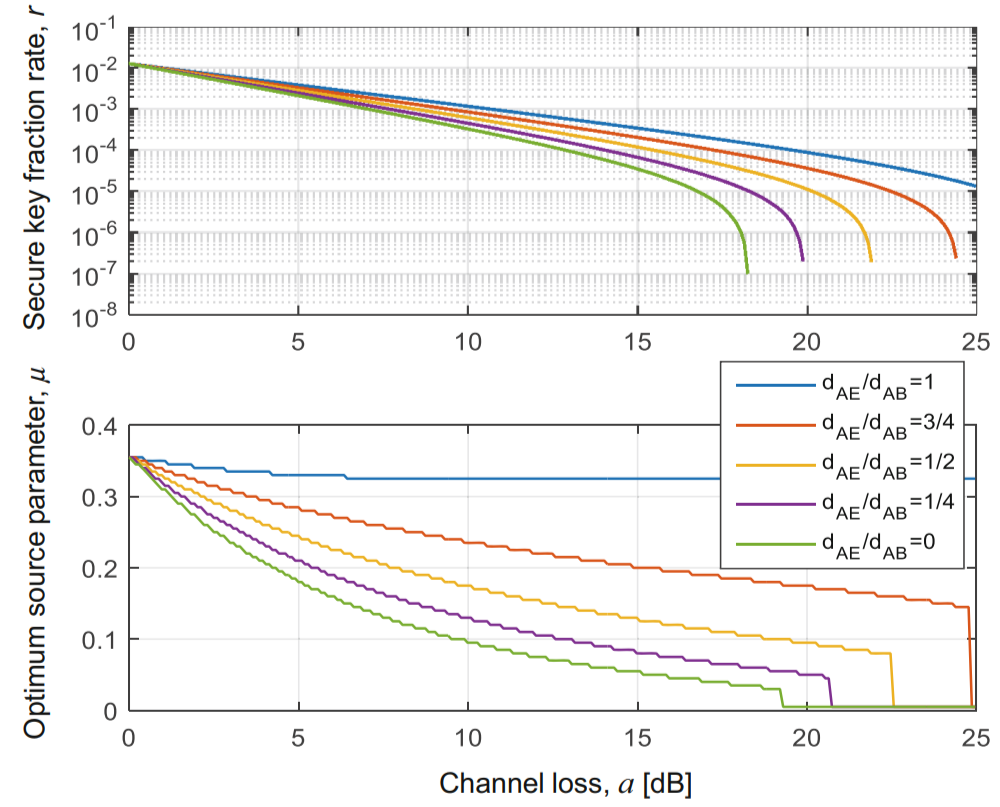
\includegraphics[width=\textwidth]{chapters/figs/fig-8-2}
	\caption{(بالا) نرخ کسر مخفی برحسب تلفات کانال به دسی‌بل، در حالی که ایو در فواصل مختلف از سمت باب ($d_{AE}/d_{AB} = 1$) تا سمت آلیس ($d_{AE}/d_{AB} = 0$) قرار دارد. (پایین) شدت منبع بهینه $\mu$ برحسب تلفات کانال (همچنین برحسب دسی‌بل). در محاسبات، پارامترها به‌صورت زیر انتخاب شده‌اند: $T_{\text{Alice}} = 0.4725$، $T_{Rx} = 0.7884$، $\eta_B = 0.898$، $\eta_{\text{det}} = 0.4352$، $\eta_{Qeff} = 0.9$، $\alpha = 0.192 \text{ dB/km}$، $p_b = 10^{-5}$، $f_{EC} = 1.16$، $N = 10^8$، $\epsilon_c = \epsilon_s = 10^{-6}$. (برگرفته از مرجع \cite{8-21}).}
	\label{fig:8-2}
\end{figure}

همان‌طور که از شکل پیداست، با افزایش تلفات کانال، هر دو مقدارِ نرخ کسر امن و پارامتر بهینه $\mu$ کاهش می‌یابند. با کاهش فاصله بین آلیس و ایو ($d_{AE}$)، که به معنای نزدیک‌تر شدن ایو به آلیس و کاهش نسبت $d_{AE}$ به کل فاصله $d_{AB}$ از ۱ (ایو در سمت باب) به ۰ (ایو در سمت آلیس) است، شدت منبع بهینه $\mu$ و در نتیجه نرخ کسر امن نیز کاهش می‌یابند.

اکنون مدل کانال متلاطم \lr{FSO} متغیر با زمان را شرح می‌دهیم \cite{8-21, 8-43}. باریکه نور هنگام انتشار در یک کانال \lr{FSO} متغیر با زمان، به دلیل توزیع تصادفی ضریب شکست، دچار اختلالات فاز و شدت می‌شود که با عنوان تلاطم\LTRfootnote{Turbulence} شناخته می‌شود \cite{8-43, 8-44, 8-45}. نوسان شدت یا تابش\LTRfootnote{Irradiance fluctuation} معمولاً به‌عنوان سنتیلاسیون\LTRfootnote{Scintillation} (چشمک‌زنی) شناخته می‌شود. اثر سنتیلاسیون در کانال‌های \lr{FSO} به‌طور گسترده مورد مطالعه قرار گرفته است تا تابع چگالی احتمال (\lr{PDF}) نوسانات تصادفی تابش استخراج شود. توزیع گاما-گاما ($\Gamma-\Gamma$) به‌عنوان مدل مناسبی برای سنتیلاسیون نوری در گستره رژیم‌های تلاطم ضعیف تا قوی عمل می‌کند که به‌صورت زیر داده می‌شود \cite{8-43, 8-44, 8-45}:

\begin{equation}
	p(I) = \frac{2 (\alpha\beta)^{(\alpha+\beta)/2}}{\Gamma(\alpha)\Gamma(\beta)} I^{(\alpha+\beta)/2 - 1} K_{\alpha-\beta} \left[ 2 (\alpha\beta I)^{1/2} \right], \quad I > 0,
	\label{eq:8-49}
\end{equation}

که در آن $I$ تابش نرمالیزه شده در گیرنده، $\Gamma(\cdot)$ تابع گاما و $K_p(\cdot)$ تابع بسل اصلاح‌شده\LTRfootnote{Modified Bessel function} نوع دوم و مرتبه $p$ است. پارامترهای $\alpha$ و $\beta$ به‌ترتیب نشان‌دهنده تعداد مؤثر سلول‌های مقیاس‌بزرگ و سلول‌های مقیاس‌کوچک در فرآیند پراکندگی هستند و به‌عنوان توابعی از واریانس ریتوف\LTRfootnote{Rytov variance} $\sigma^2_R$ تعریف می‌شوند که معمولاً به‌عنوان معیاری برای شدت تلاطم اتمسفری استفاده می‌شود. برای بررسی رابطه آن‌ها با واریانس ریتوف در حالت مقیاس درونی غیرصفر، خواننده علاقه‌مند به مرجع \cite{8-21} ارجاع داده می‌شود. تلاطم ضعیف با $\sigma^2_R < 1$، تلاطم متوسط با $\sigma^2_R \sim 1$ و رژیم تلاطم قوی با $\sigma^2_R > 1$ مشخص می‌شوند. رژیم موسوم به اشباع\LTRfootnote{Saturation regime} نیز با شرط $\sigma^2_R \to \infty$ تعیین می‌گردد.

برای مشخصه‌یابی فرکانسی سنتیلاسیون نوری، نوسانات شدت در بازه زمان همدوسی\LTRfootnote{Coherence time} اتمسفری به‌شدت همبسته هستند. زمان همدوسی که با $\tau_c$ نشان داده می‌شود، به‌عنوان حداقل مدت‌زمانی تعریف می‌شود که طی آن دو نمونه متوالی از شدت دریافتی ناهمبسته باشند. مطالعات بسیاری برای مدل‌سازی چگالی طیفی توان\LTRfootnote{Power spectral density (PSD)} (\lr{PSD}) سنتیلاسیون نوری برای هر دو مسیر افقی و عمودی انجام شده است، مانند \cite{8-46, 8-47}. مشخص شده است که طیف سنتیلاسیون مستقیماً با سرعت باد در طول کانال مرتبط است. فرمول‌های کلی در مرجع \cite{8-45} برای طیف‌های فرکانس زمانی سنتیلاسیون نوری برای هر دو نوع موج تخت و موج باریکه گاوسی ارائه شده است. \lr{PSD} برای محیط‌های مختلف از مکانی به مکان دیگر تغییر می‌کند و تحت تأثیر پارامترهای شرایط آب‌وهوایی مانند دما و رطوبت قرار می‌گیرد. یک مدل طیفی ساده از نوع باترورث\LTRfootnote{Butterworth-type} برای پیوندهای \lr{FSO} زمینی، که توسط دو پارامترِ فرکانس قطع و شیب طیفی تعیین می‌شود، در مرجع \cite{8-47} پیشنهاد شده است. این تابع انتقال توان به‌خوبی با شکل \lr{PSD} سنتیلاسیون نوری که از داده‌های تجربی برای یک پیوند افقی ۱ کیلومتری در یک محیط زمینی شهری استخراج شده است، مطابقت دارد \cite{8-47}. ما از این مدل باترورث مرتبه اول با فرکانس قطع $12$ هرتز در مدل کانال \lr{FSO} استفاده می‌کنیم تا به زمان همدوسی کانال در حدود $\tau_c \sim 10$ میلی‌ثانیه دست یابیم. برای به‌دست آوردن سنتیلاسیون نوری تحت تلاطم قوی، ابتدا دنباله‌ای از نمونه‌های تصادفی با توزیع نرمال ناهمبسته تولید کرده و سپس دنباله را توسط فیلتر باترورث فیلتر می‌کنیم. سپس هر نمونه را از توزیع نرمال به یک توزیع گاما-گاما (رابطه \eqref{eq:8-49}) با واریانس ریتوف $\sigma^2_R = 30$ با استفاده از تکنیک تبدیل غیرخطی بدون حافظه\LTRfootnote{Memoryless non-linear transform (MNLT)} (\lr{MNLT}) \cite{8-48} نگاشت می‌دهیم؛ این تکنیک با برابر قرار دادن توابع توزیع انباشته\LTRfootnote{Cumulative density functions (CDF)} (\lr{CDF}) آن‌ها، داده‌ها را از توزیع نرمال به توزیع گاما-گاما نگاشت می‌کند که در آن همبستگی موجود در دنباله حفظ می‌شود.








\lr{PSD}\LTRfootnote{Power Spectral Density} و \lr{PDF}\LTRfootnote{Probability Density Function} مدل کانال \lr{FSO} متغیر با زمان به‌ترتیب در شکل‌های \ref{fig:8-3} (\subref{fig:8-3-a} و \subref{fig:8-3-b}) نشان داده شده‌اند. زمان همدوسی\LTRfootnote{Coherence time} همان‌طور که هدف‌گذاری شده بود، تقریباً $10$ میلی‌ثانیه است. ما با فرض اینکه کانال در طول زمان همدوسی ثابت است (زیرا نمونه‌های شدت به‌شدت همبسته هستند)، مدل سنتیلاسیون\LTRfootnote{Scintillation} را به یک مدل محوشدگی بلوکی\LTRfootnote{Block fading} متغیر با زمان ساده می‌کنیم. همان‌طور که در شکل \ref{fig:8-3} (\subref{fig:8-3-b}) مشاهده می‌شود، \lr{PDF} مدل محوشدگی بلوکی به‌خوبی با توزیع تئوری گاما-گاما مطابقت دارد. ما همچنین فرض می‌کنیم که نوسانات در شدت دریافتی کاملاً ناشی از نوسانات در گذردهی کانال هستند؛ بنابراین بازدهی ارسال کانال، به‌عنوان مثال گذردهی کانال $\bm{T}$، با تابش دریافتی متناسب است که می‌تواند به‌عنوان حاصل‌ضرب گذردهی میانگین و توان دریافتی نرمالیزه‌شده‌ی حاصل از مدل محوشدگی بلوکی محاسبه شود.

\begin{figure}[ht]
	\centering
	\subfigure[]{\label{fig:8-3-a}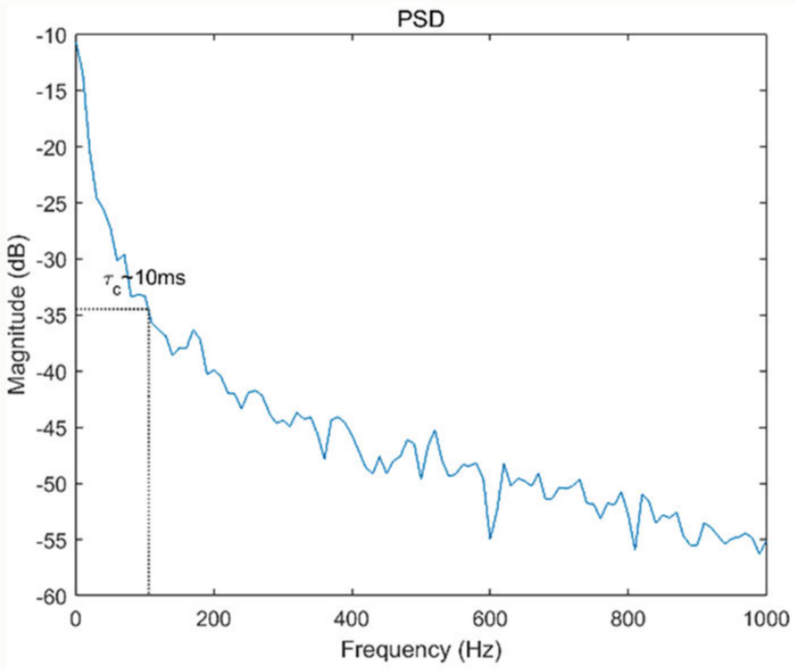
\includegraphics[width=0.48\textwidth]{chapters/figs/fig-8-3-a}}
	\hfill
	\subfigure[]{\label{fig:8-3-b}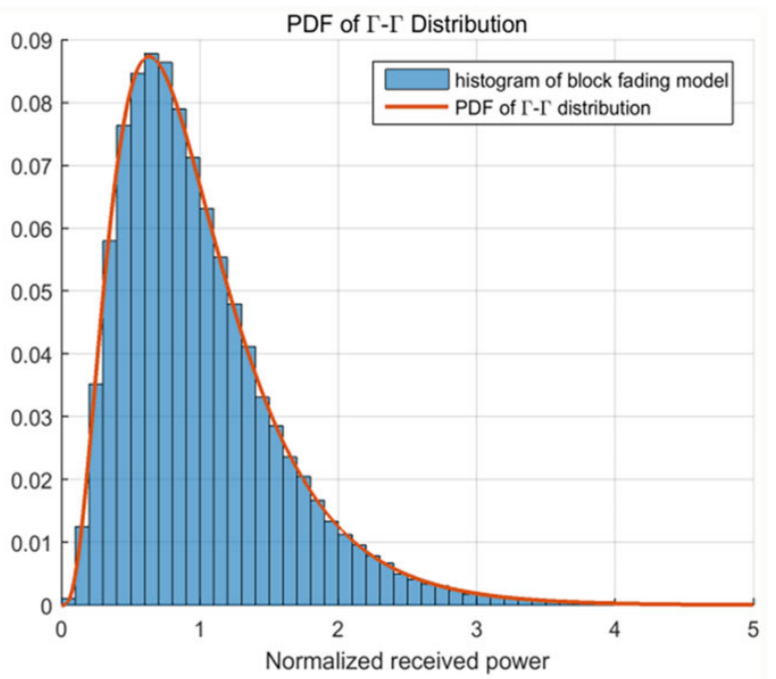
\includegraphics[width=0.48\textwidth]{chapters/figs/fig-8-3-b}}
	\caption{مدل کانال متغیر با زمان: (\subref{fig:8-3-a}) \lr{PSD} مدل محوشدگی بلوکی تولیدشده؛ (\subref{fig:8-3-b}) \lr{PDF} توزیع گاما-گاما با واریانس ریتوف $30$ و هیستوگرام مدل محوشدگی بلوکیِ تابش دریافتی نرمالیزه‌شده. (برگرفته از مرجع \cite{8-21}).}
	\label{fig:8-3}
\end{figure}

عملکرد نرخ‌های کسر امن در سیستم \lr{QKD} مبتنی بر \lr{FSO} می‌تواند به‌طور قابل‌توجهی تحت تأثیر اثرات تلاطم اتمسفری قرار گیرد. به‌طور معمول، اغلب بر اساس شرایط میانگین کانال، یک شدت منبع ثابت فرض می‌شد، در حالی که ماهیت متغیر با زمانِ کانال \lr{FSO} عموماً نادیده گرفته می‌شود. بنابراین، در حضور تلاطم، توان ارسال ثابت اغلب نسبت به گذردهی آنی کانال دارای عدم انطباق\LTRfootnote{Mismatch} بوده و در نتیجه منجر به کاهش امنیت می‌گردد.






برای مواجهه با شرایط متغیر زمانی کانال \lr{FSO}، ما یک روش تطبیقی را پیشنهاد دادیم که در آن کانال \lr{FSO} را با یک سیگنال کاوشگر کلاسیک کمکی پایش کرده، سپس حالات کانال را بر اساس حالات قبلی و فعلی پیش‌بینی می‌کنیم و درخشندگی منبع را مطابق با پیش‌بینی‌های کانال تطبیق می‌دهیم تا نرخ‌های کسر امن بهبود یابند \cite{8-21}. در یک سیستم \lr{FSO} واقع‌گرایانه، ممکن است تأخیری بین اندازه‌گیری حالت کانال و اعمال تنظیمات بر پارامترهای منبع وجود داشته باشد که می‌تواند ناشی از تأخیر انتشار فیزیکی در طول مسیر یا به دلیل برخی فرآیندهای پردازش سیگنال در سیستم باشد. در چنین حالتی، پیش‌بینی حالات کانال به‌صورت بی‌درنگ\LTRfootnote{Real-time} ضروری است. در روش تطبیقی ما، یک پیش‌بین خودواگرد\LTRfootnote{Autoregressive (AR) predictor} (\lr{AR}) در سمت آلیس برای پیش‌بینی اطلاعات وضعیت کانال استفاده می‌شود و دقت پیش‌بینی‌ها تعیین می‌کند که تا چه حد بهبود در این طرح تطبیقی حاصل می‌شود. یک مدل \lr{AR} را می‌توان به‌عنوان یک فیلتر با پاسخ ضربه نامحدود\LTRfootnote{Infinite impulse response (IIR)} (\lr{IIR}) در نظر گرفت و مسئله اصلی، تعیین ضرایب فیلتر به‌گونه‌ای است که میانگین مربعات خطا کمینه شود. طبق تعریف، یک مدل خودواگرد به‌صورت زیر داده می‌شود:
\begin{equation}
	y_t = \sum_{i=1}^{o} a_i y_{t-i} + \epsilon_t,
	\label{eq:8-50}
\end{equation}
که در آن $a_i$ ضرایب خودواگرد ($i = 1, \dots, o$)، متغیر $y_t$ نشان‌دهنده حالات متوالی کانال متغیر با زمان، $o$ مرتبه مدل و $\epsilon_t$ نشان‌دهنده خطای باقی‌مانده است که یک فرآیند نویز سفید با میانگین صفر فرض می‌شود. با استفاده از مدل \lr{AR} فوق، هر حالت کانال $y_t$ را می‌توان از روی $o$ حالت قبلی به‌صورت زیر پیش‌بینی کرد:
\begin{equation}
	\hat{y}_t = \sum_{i=1}^{o} a_i y_{t-i},
	\label{eq:8-51}
\end{equation}
که در آن $\hat{y}_t$ نشان‌دهنده تخمینی از حالت کانال $y_t$ است. خطای پیش‌بینی به‌صورت تفاضل بین حالت تخمینی و واقعی کانال تعریف می‌شود، یعنی $\epsilon_t = y_t - \hat{y}_t$. با افزایش مرتبه مدل \lr{AR}، عملکرد پیش‌بین بهبود می‌یابد. برای ارزیابی دقت روش \lr{AR}، معمولاً از ریشه میانگین مربعات خطا\LTRfootnote{Root mean square error (RMSE)} (\lr{RMSE}) بین مقادیر پیش‌بینی‌شده و واقعی حالات کانال استفاده می‌شود، همان‌طور که در شکل \ref{fig:8-4} تصویر شده است. ما یک پیش‌بین $AR(o)$ را بر اساس مدل محوشدگی بلوکی که پیش‌تر شرح داده شد مدل‌سازی کرده و پیش‌بینی تک‌گامه یا چندگامه را با مرتبه حداکثر $20$ انجام می‌دهیم. همان‌طور که در شکل \ref{fig:8-4} (\subref{fig:8-4-a}) نشان داده شده است، مقدار \lr{RMSE} در مرتبه $o = 3$ به‌سرعت افت کرده و سپس با افزایش مرتبه فیلتر به‌کندی کاهش می‌یابد. طول پیش‌بینی $K$ بر دقت پیش‌بینی تأثیر می‌گذارد که در شکل \ref{fig:8-4} (\subref{fig:8-4-b}) با عنوان پیش‌بینی «$K$-گام-جلوتر» نشان داده شده است. همان‌طور که انتظار می‌رفت، با افزایش طول پیش‌بینی، مقدار \lr{RMSE} افزایش می‌یابد.

\begin{figure}[ht]
	\centering
	\subfigure[]{\label{fig:8-4-a}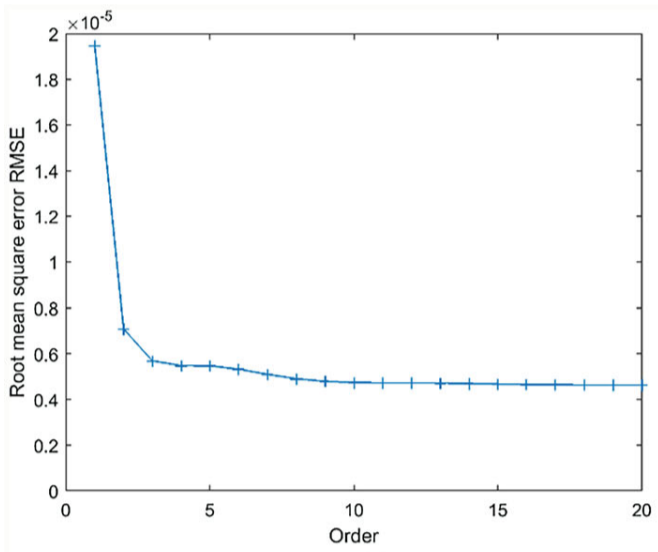
\includegraphics[width=0.45\textwidth]{chapters/figs/fig-8-4-a}}
	\hfill
	\subfigure[]{\label{fig:8-4-b}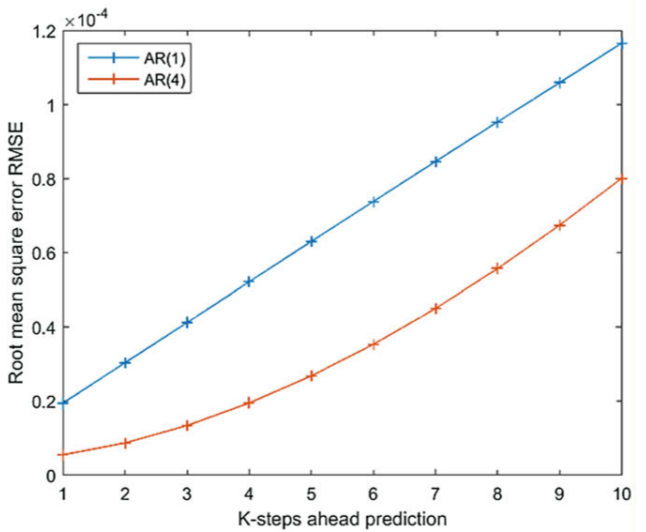
\includegraphics[width=0.45\textwidth]{chapters/figs/fig-8-4-b}}
	\caption{(\subref{fig:8-4-a}) ریشه میانگین مربعات خطا (\lr{RMSE}) برحسب مرتبه مدل \lr{AR}. (\subref{fig:8-4-b}) مقدار \lr{RMSE} برحسب طول پیش‌بینی $K$.}
	\label{fig:8-4}
\end{figure}

یک نمونه از بهبود حاصل از روش تطبیقی ما در شکل \ref{fig:8-5} تصویر شده است. در محاسبات، فرض کردیم که ایو در سمت آلیس قرار دارد ($d_{AE}/d_{AB} = 0$). منحنی آبی در وسط مربوط به نرخ کسر امن برای گذردهی میانگین کانال $T = T_{abs} T_{scatt}$ است که در آن گذردهی‌های جذب ($T_{abs}$) و پراکندگی ($T_{scatt}$) به‌ترتیب روی $0.9917$ و $0.365$ تنظیم شده‌اند. برای این مقدار میانگین، شدت منبع بهینه $\mu = 0.195$ برای بیشینه‌سازی نرخ کسر امن انتخاب شده است. زمانی که کانال \lr{FSO} در محوشدگی عمیق قرار دارد، همان‌طور که توسط منحنی زرد نشان داده شده است، باید درخشندگی منبع را برای تضمین امنیت کاهش دهیم. شدت بهینه به مقدار جدید $\mu = 0.135$ تغییر می‌کند. به‌سادگی از شکل دیده می‌شود که با کار در مقدار بهینه جدید، نرخ کسر امن از خط‌چین سیاه به خط‌چین خاکستری بهبود می‌یابد. مشابه بدترین حالت، زمانی که شرایط کانال بهتر می‌شود (مانند منحنی قرمز در بالا)، تطبیق شدت منبع با مقدار بهینه بالاترِ جدید $\mu = 0.25$ نیز باعث افزایش \lr{SKR} می‌گردد. به‌طور خلاصه، روش تطبیقی به منبع اجازه می‌دهد تا در درخشندگی بهینه (یا زیربهینه در صورتی که پیش‌بینی‌های وضعیت کانال خیلی دقیق نباشند) عمل کند.

\begin{figure}[ht]
	\centering
	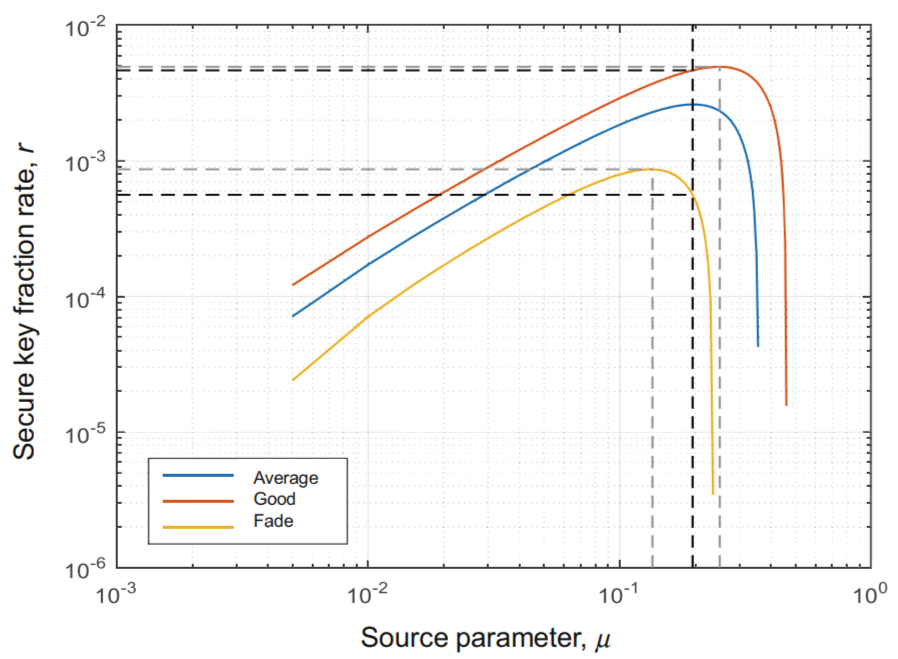
\includegraphics[width=0.8\textwidth]{chapters/figs/fig-8-5}
	\caption{تصویرسازی بهبود در نرخ کسر امن از طریق تطبیق درخشندگی منبع مبتنی بر مدل \lr{AR}. (برگرفته از مرجع \cite{8-21}).}
	\label{fig:8-5}
\end{figure}

با به‌کارگیری روش تطبیقی مبتنی بر مدل \lr{AR}، ما \lr{QKD} مبتنی بر \lr{BB84} را برای منبع همدوس ضعیف تحت رژیم تلاطم قوی با مدل‌سازی کانال \lr{FSO} متغیر با زمان به‌صورت مدل محوشدگی بلوکی شبیه‌سازی می‌کنیم. در اینجا از همان پارامترهای معرفی‌شده در بالا استفاده می‌کنیم. یک مدل ساده $AR(1)$ مرتبه اول، که توسط $1000$ نمونه اول در مدل کانال آموزش دیده است، برای پیش‌بینی حالات کانال در یک زمان همدوسی ($\tau_c$) و پنج زمان همدوسی جلوتر استفاده می‌شود. نرخ کسر امن با استفاده از رابطه \eqref{eq:8-48} برای هر زمان همدوسی محاسبه شده و سپس روی کل پالس‌های سیگنال ارسالی $N$ میانگین‌گیری می‌شود؛ نتایج عددی متناظر در شکل \ref{fig:8-6} خلاصه شده‌اند. روش تطبیق درخشندگی منبع در واقع نرخ کسر امن را در مقایسه با حالتی که از شدت منبع ثابت $\mu = 0.195$ (که برای شرایط میانگین کانال بهینه است) استفاده می‌شود، افزایش می‌دهد. برای منحنی «پیش‌بینی‌های کامل»، ما نرخ کسر امن را با این فرض تعیین می‌کنیم که حالات کانال به‌طور کامل پیش‌بینی شده‌اند. اگرچه چالش‌های فناورانه اساسی در ایجاد منابع تک‌فوتونی برحسب تقاضا همچنان امکان \lr{BB84} «خالص» را در نرخ داده‌های بالایی که در اینجا مد نظر ماست محدود می‌کند، اما هنگام مقایسه با نرخ کسر امنِ \lr{BB84} ایده‌آل با استفاده از منابع تک‌فوتونی، روش تطبیقی ما شکافِ ناشی از استفاده از منابع \lr{WCS} تجاری را کاهش می‌دهد. نسبت بهبود در نرخ کسر امن برای مورد جبران‌سازی کامل در پایین شکل \ref{fig:8-6} نشان داده شده است. علاوه‌بر این، عملکرد تطبیق درخشندگی منبع مبتنی بر روش \lr{AR} به دقت پیش‌بینی‌های حالت کانال بستگی دارد. با کاهش دقت پیش‌بینی هنگام افزایش طول پیش‌بینی، نرخ کسر امن در مقایسه با حالت ایده‌آل پیش‌بینی کامل کاهش می‌یابد. نرخ کسر امن متناظر با پیش‌بینی یک زمان همدوسی جلوتر، به‌طور نزدیکی به حالت پیش‌بینی کامل میل می‌کند.

\begin{figure}[ht]
	\centering
	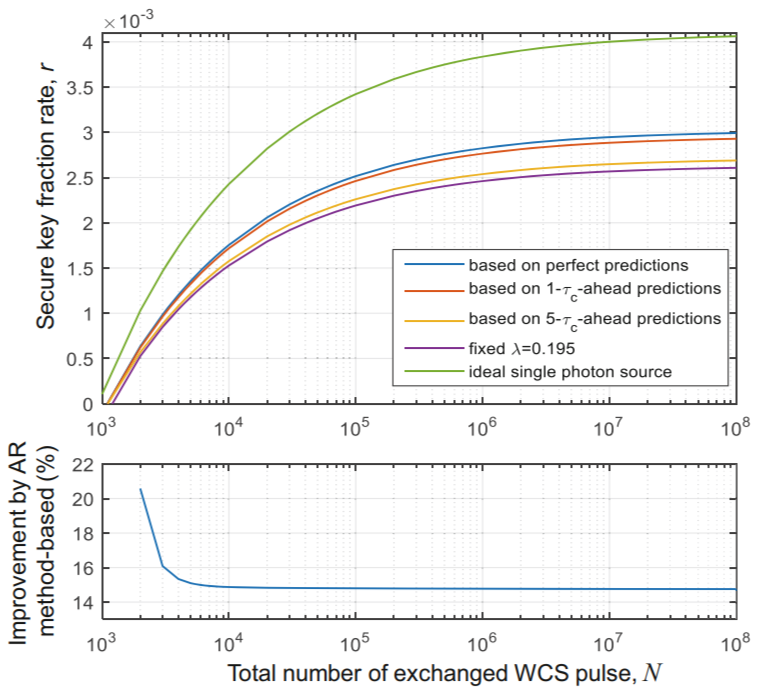
\includegraphics[width=0.8\textwidth]{chapters/figs/fig-8-6}
	\caption{بهبود در تطبیق مبتنی بر پیش‌بین \lr{AR}: (بالا) نرخ کسر امن برحسب تعداد کل پالس‌های \lr{WCS} مبادله‌شده ($N$)؛ (پایین) نسبت بهبود برای جبران‌سازی کامل برحسب $N$. (برگرفته از مرجع \cite{8-21}).}
	\label{fig:8-6}
\end{figure}

\subsubsection{پروتکل حالت فریب روی کانال‌های FSO متغیر با زمان}
\label{subsec:8-3-2}
برای بهینه‌سازی پروتکل مبتنی بر حالت فریب، ما از توصیف پروتکل ارائه شده در مرجع \cite{8-49} پیروی می‌کنیم. در این بخش، یک پروتکل حالت فریب مبتنی بر \lr{BB84} با سه حالت مختلف (یک حالت سیگنال و دو حالت فریب) مطالعه می‌شود. در مرجع \cite{8-50} نشان داده شده است که بهبود در نرخ کسر امن هنگام به‌کارگیری بیش از دو حالت فریب (علاوه بر حالت سیگنال) کمتر از $1\%$ است. در اینجا، ما از $\mu = \{\mu_1, \mu_2, \mu_3\}$ برای نشان دادن سه حالت مورد استفاده در پروتکل، و از $\lambda = \{\lambda_1, \lambda_2, \lambda_3\}$ برای نشان دادن شدت‌های منبع متناظر استفاده می‌کنیم. هر حالت با احتمال $p_{\mu_1} > p_{\mu_2} > p_{\mu_3} = 1 - p_{\mu_1} - p_{\mu_2}$ انتخاب می‌شود. با پیروی از تکنیک اثبات امنیت طول کلید محدود برای پروتکل مبتنی بر حالت‌های فریب بر اساس رابطه عدم قطعیت برای آنتروپی‌های هموار \cite{8-28, 8-29, 8-41, 8-51}، نرخ کسر کلید امن برای یک پروتکل حالت فریب با پایه‌های بدون سوگیری، که در آن دو پایه متقابل به‌طور یکسان انتخاب می‌شوند، به‌صورت زیر داده می‌شود:
\begin{equation}
	r \leq \frac{1}{2} \left[ \underline{Q}^{(0)} + \underline{Q}^{(1)} - \overline{Q}^{(1)} h(\bar{e}^{(1)}) - \frac{\text{leak}_{EC}}{N} - \Delta(N) \right],
	\label{eq:8-52}
\end{equation}
که در آن کران پایین و کران بالا به‌ترتیب با خط زیرین و خط بالایی نشان داده شده‌اند. در رابطه \eqref{eq:8-52}، $Q^{(n)}$ نشان‌دهنده نرخ آشکارسازی در سمت باب است که ناشی از سیگنال‌های با $n$ فوتون گسیل‌شده از منبع آلیس می‌باشد. با $e$ نرخ کل \lr{QBER} و با $e^{(n)}$ نرخ \lr{QBER} برای پالس‌های $n$-فوتونی را نشان داده‌ایم. مشابه قبل، $h_2(x)$ نشان‌دهنده تابع آنتروپی باینری است. پارامتر $\text{leak}_{EC}$ متناظر با نشت اطلاعات ناشی از تصحیح خطا (مصالحه اطلاعات) است. این بخش از اطلاعات باید هنگام محاسبه نرخ کسر امن کسر شود، زیرا ایو می‌تواند این بیت‌ها را صرفاً با انشعاب گرفتن از کانال کلاسیک تعیین کند. معمولاً این مقدار به‌صورت $\text{leak}_{EC} \approx Q f_{EC} h(e)$ تقریب زده می‌شود که در آن $Q$ نرخ کل آشکارسازی و $f_{EC}$ ناکارآمدی تصحیح خطا است. آخرین جمله در رابطه \eqref{eq:8-52} یعنی $\Delta(N)$، مربوط به امنیت تحت اثر اندازه محدود است که به‌صورت زیر تخمین زده می‌شود:
\begin{equation}
	\Delta(N) = \frac{1}{N} \log_2 \left( \frac{2}{\epsilon_c} \right) + \frac{6}{N} \log_2 \left( \frac{46}{\epsilon_s} \right).
	\label{eq:8-53}
\end{equation}
مشابه بخش قبلی، پروتکل \lr{QKD} مبتنی بر حالت‌های فریب زمانی $\epsilon$-امن (یا به‌طور دقیق‌تر $\epsilon_c$-صحیح و $\epsilon_s$-محرمانه) نامیده می‌شود که $\epsilon \geq \epsilon_s + \epsilon_c$ باشد. کران‌های پایین و بالا در رابطه \eqref{eq:8-52} با استفاده از نامساوی هوفدینگ\LTRfootnote{Hoeffding’s inequality} \cite{8-52} و بهینه‌سازی مقید تعیین می‌شوند. به‌طور مشخص‌تر، مقادیر قابل اندازه‌گیری در پروتکل، مانند تعداد آشکارسازی‌ها و تعداد خطاها، توسط نامساوی هوفدینگ از مقادیر مجانبی محدود می‌شوند: $x_{asym} - x \leq \sqrt{(x/2) \ln(1/\epsilon)}$ با احتمال شکست $2\epsilon$. سپس این کران‌ها به‌عنوان محدودیت‌های مسئله بهینه‌سازی برای تخمین مقادیری که مستقیماً قابل اندازه‌گیری نیستند، استفاده می‌شوند. برای مثال، از برنامه‌ریزی خطی برای به‌دست آوردن نرخ آشکارسازی سیگنال‌های $n$-فوتونی $\underline{q}_{\mu_i}^{(n)}$، که از پالس‌های آماده‌شده توسط آلیس در حالت $\mu_i$ ناشی می‌شوند، استفاده می‌شود:
\begin{equation}
	\min \underline{q}_{\mu_i}^{(n)},
	\label{eq:8-54}
\end{equation}
تحت قیود:
\begin{equation}
	\begin{aligned}
		\underline{Q}_{\mu_i} \leq \sum_{n=0}^{\infty} q_{\mu_i}^{(n)} e^{-\lambda_i} \frac{\lambda_i^n}{n!} \leq \overline{Q}_{\mu_i}, \quad n \in \{0, 1\}, \quad i \in \{1, 2, 3\} \\
		0 \leq q_{\mu_i}^{(n)} \leq 1, \quad n \in \{0, 1\}, \quad i \in \{1, 2, 3\}
	\end{aligned}
	\label{eq:8-55}
\end{equation}
که در آن $Q_{\mu_i} = C_{\mu_i} / N_{\mu_i}$ نرخ آشکارسازی برای هر حالت $\mu_i$ است، و $C_{\mu_i}$ و $N_{\mu_i}$ به‌ترتیب تعداد کل سیگنال‌هایی هستند که در حالت $\mu_i$ آشکار و ارسال شده‌اند. سپس کران‌های نرخ آشکارسازی پالس‌های $n$-فوتونی به‌صورت $\underline{Q}^{(n)} = \left[ \frac{N_{\mu_i}}{N} \underline{q}_{\mu_i}^{(n)} e^{-\lambda_i} \frac{\lambda_i^n}{n!} \right]$ داده می‌شود. مسئله بهینه‌سازی برای کران بالای \lr{QBER} تک‌فوتونی $\bar{e}^{(1)}$ را می‌توان با رابطه زیر ساده کرد \cite{8-53}:
\begin{equation}
	\bar{e}^{(1)} \leq \frac{e^{\lambda_i} e_{\mu_i} - \frac{1}{2} \underline{q}_{\mu_i}^{(0)}}{\lambda_i \underline{q}_{\mu_i}^{(1)}},
	\label{eq:8-56}
\end{equation}
که در آن $e_{\mu_i} = E_{\mu_i} / N_{\mu_i}$ نرخ \lr{QBER} از هر حالت $\mu_i$ است و $E_{\mu_i}$ تعداد کل خطاهایی است که در حالت $\mu_i$ آشکار شده‌اند. بهینه‌سازی عددی برای تعیین پارامترهای بهینه پروتکل حالت‌های فریب انجام شده است که نتایج عددی آن در شکل \ref{fig:8-7} برای تعداد کل پالس‌های سیگنال مبادله‌شده $N = 10^8$ خلاصه شده است. به‌وضوح، شدت منبع برای حالت سیگنال نیازی به کاهش خطی با گذردهی کانال ندارد و مقدار بهینه در سطح نسبتاً بالای $\lambda \sim 1$ باقی می‌ماند. با افزایش تلفات کانال، به دلیل پایین بودن نرخ آشکارسازی، حالت‌های فریب قوی‌تر برای تخمین آمار تک‌فوتونی بیشتر مورد نیاز هستند. توجه داشته باشید که نتایج عددی ما نشان می‌دهند که یکی از حالت‌های فریب همیشه در شدت صفر بهینه است، که با تحلیل مرجع \cite{8-54} که چنین حالتی را «حالت فریب خلاء» می‌نامد، مطابقت دارد.
%
\begin{figure}[ht]
	\centering
	\subfigure[]{\label{fig:8-7-a}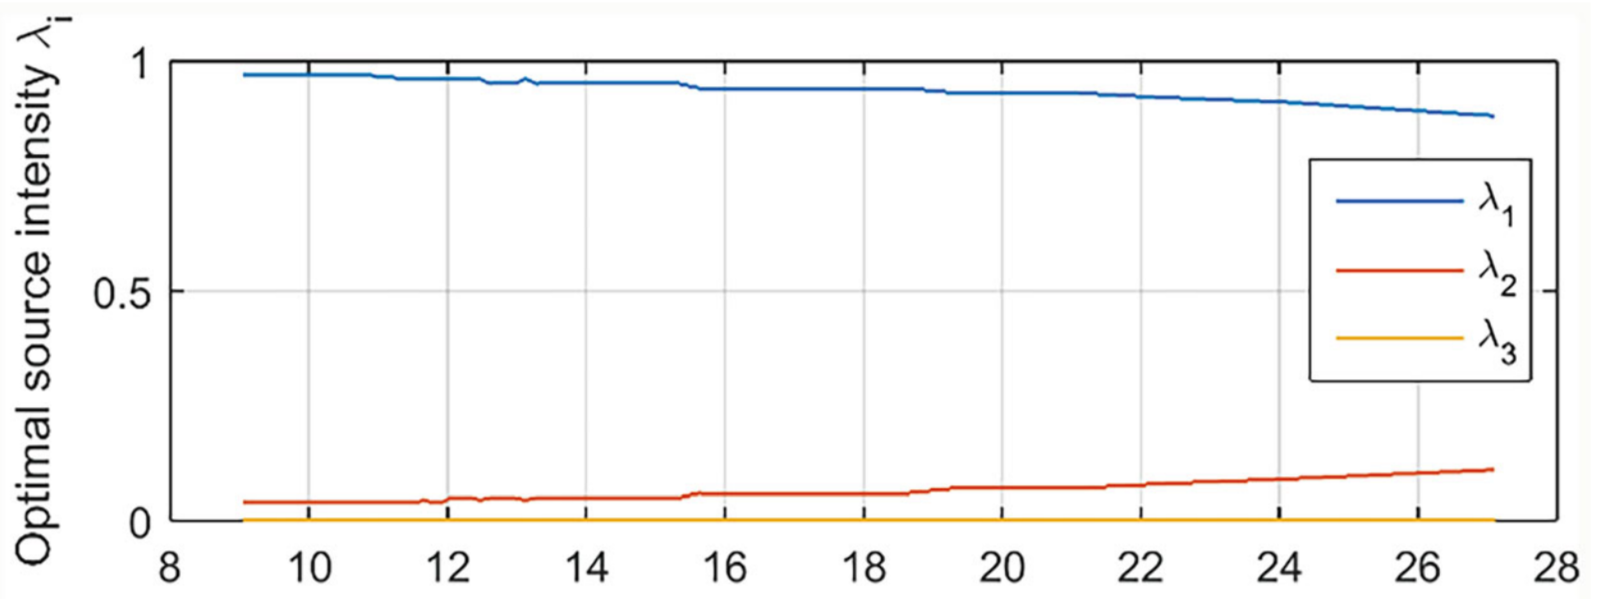
\includegraphics[width=.8\textwidth]{chapters/figs/fig-8-7-a}}
	
	
	\subfigure[]{\label{fig:8-7-b}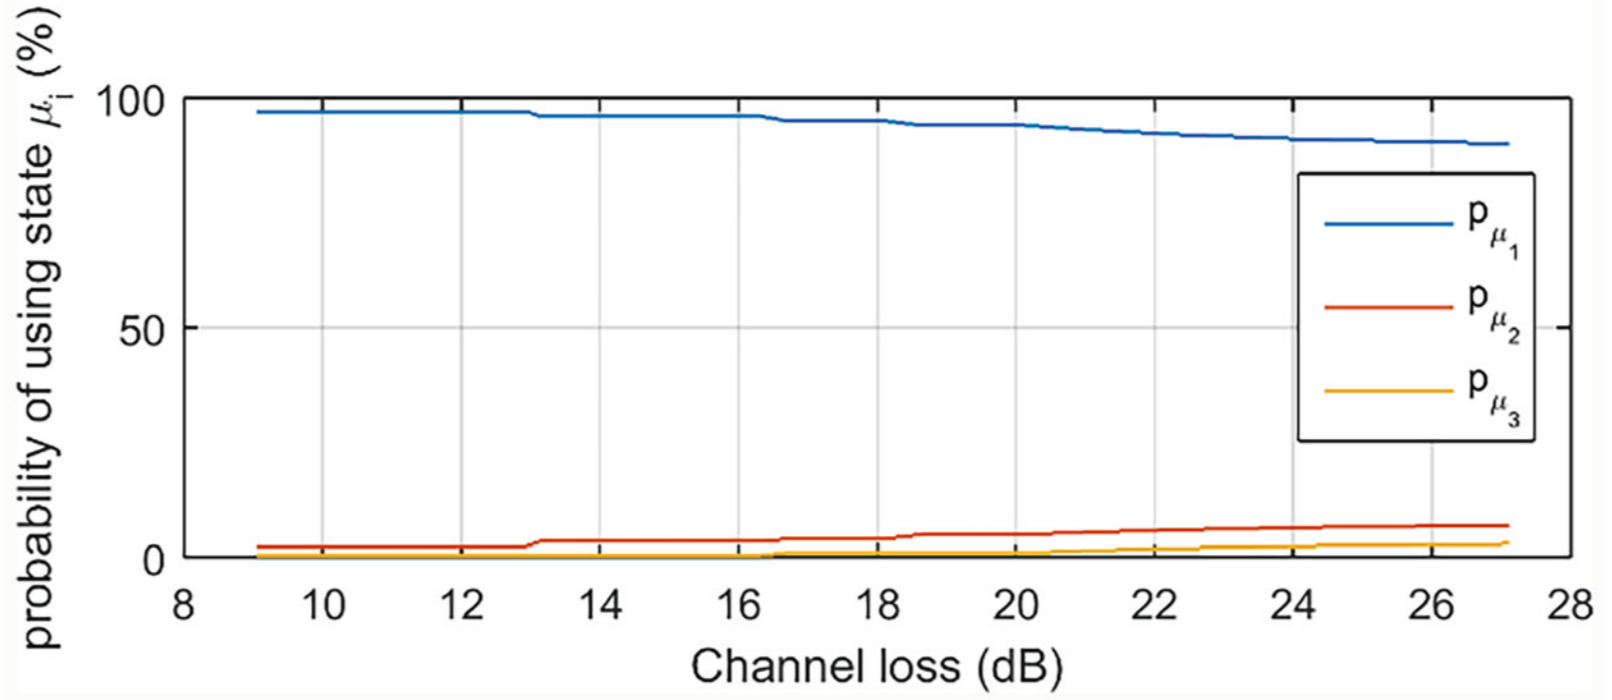
\includegraphics[width=0.8\textwidth]{chapters/figs/fig-8-7-b}}
	\caption{پارامترهای بهینه پروتکل دو-حالت-فریب در مقابل تلفات آنی کانال ناشی از تلاطم: (\subref{fig:8-7-a}) شدت منبع بهینه برحسب تلفات کانال به دسی‌بل؛ (\subref{fig:8-7-b}) احتمال ($\%$) استفاده آلیس از هر حالت برحسب تلفات کانال. (برگرفته از مرجع \cite{8-21}).}
	\label{fig:8-7}
\end{figure}

مشابه \lr{BB84} مبتنی بر \lr{WCS}، \lr{QKD} حالت فریب مبتنی بر \lr{FSO} نیز تحت تأثیر اثرات تلاطم اتمسفری قرار می‌گیرد. ما پروتکل حالت فریب شرح داده شده در بالا را تحت تلاطم قوی با تطبیق مبتنی بر پیش‌بین \lr{AR} شبیه‌سازی می‌کنیم. همان مقادیر امنیتی $\epsilon_c = \epsilon_s = 10^{-6}$ و نویز پس‌زمینه $p_b = 10^{-5}$ که در پروتکل \lr{BB84} مبتنی بر \lr{WCS} استفاده شده بود، در اینجا نیز به کار گرفته شده است. همان‌طور که در شکل \ref{fig:8-8} نشان داده شده است، نرخ‌های کسر امن با روش تطبیقی مبتنی بر پیش‌بین \lr{AR} بهبود می‌یابند و سطح بهبود عملکرد نرخ کسر کلید امن به دقت پیش‌بینی‌ها بستگی دارد. نرخ‌های کسر امن از بالا توسط حالت پیش‌بینی کامل محدود می‌شوند. در مقایسه با پروتکل‌های \lr{BB84}، از آنجا که نرخ کسر امن در پروتکل حالت فریب به‌صورت خطی با گذردهی کانال مقیاس‌بندی می‌شود \cite{8-55}، بهبود حاصل از تطبیق شدت منبع کمتر است. برای حالت پارامتر ثابت، پارامترهای بهینه تحت فرض مجانبی محاسبه شده‌اند؛ بنابراین همان‌طور که انتظار می‌رود، زمانی که تعداد کل پالس‌های سیگنال ارسالی $N$ بزرگ باشد، عملکرد بهتری دارد. بهبود تطبیقی برحسب نرخ کسر امن نسبت به تطبیق کامل، از $20\%$ در $N = 10^6$ به $5\%$ در $N = 10^9$ کاهش می‌یابد. مورد پیش‌بینی یک زمان همدوسی جلوتر، به‌طور نزدیکی به مورد تخمین کامل کانال میل می‌کند و برای تمام مقادیر $N$ مفید است. با این حال، دقت پیش‌بینی‌های پنج زمان همدوسی جلوتر برای تمام مقادیر $N$ در مقایسه با \lr{BB84} به اندازه کافی خوب نیست. زمانی که $N$ بزرگ است، جایی که مورد پارامتر ثابت به‌خوبی عمل می‌کند، روش تطبیقی به دلیل عدم‌انطباق ناشی از پیش‌بینی‌های ضعیف حالت کانال، منجر به نرخ کلید کسر امن پایین‌تری می‌شود. از این منظر، پروتکل حالت فریب به دقت پیش‌بینی بالاتری نسبت به \lr{BB84} اصلی نیاز دارد. به عبارت دیگر، پروتکل مبتنی بر حالت فریب در مقایسه با پروتکل \lr{BB84} نسبت به اثرات تلاطم اتمسفری صلب‌تر است، به‌طوری که تطبیق مبتنی بر پیش‌بین \lr{AR} در این مورد برای $N$ به اندازه کافی طولانی کمک چندانی نمی‌کند.

\begin{figure}[ht]
	\centering
	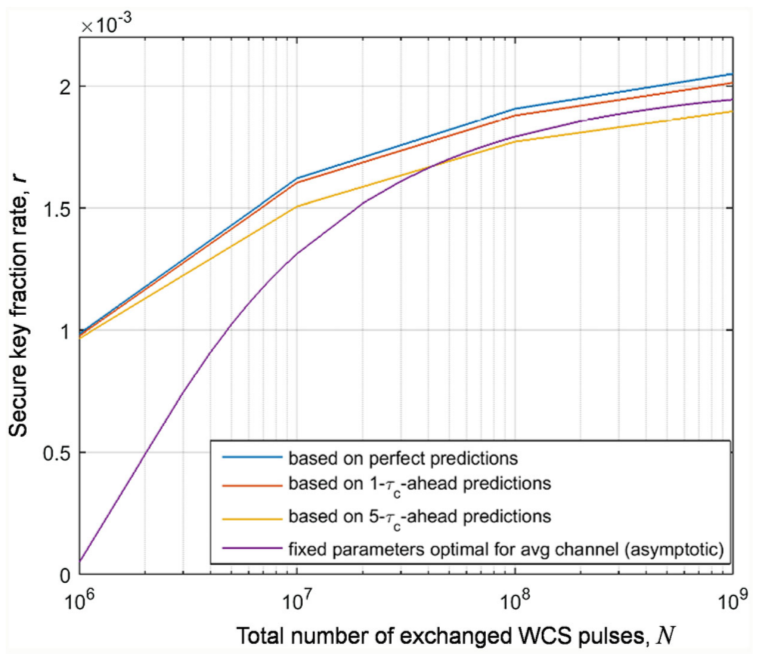
\includegraphics[width=0.8\textwidth]{chapters/figs/fig-8-8}
	\caption{نرخ کسر کلید امن برحسب تعداد کل پالس‌های سیگنال ارسالی ($N$) برای \lr{QKD} مبتنی بر حالت فریب با تطبیق مبتنی بر روش \lr{AR}. (برگرفته از مرجع \cite{8-21}).}
	\label{fig:8-8}
\end{figure}

\section{پروتکل‌های DV-QKD با ابعاد بالا}
\label{sec:8-4}
به‌رغم ویژگی‌های جذاب \lr{QKD}، دو چالش بنیادی و فنی وجود دارد که باید پیش از کاربردهای گسترده آن مورد توجه قرار گیرند. نخست، نرخ کلید مخفی \lr{QKD} به‌طور بنیادی توسط تلفات کانال محدود می‌شود، که توسط مصالحه نرخ-تلفات\LTRfootnote{Rate-loss tradeoff} کمی‌سازی می‌گردد \cite{8-56, 8-57, 8-58}. تکرارکننده‌های کوانتومی\LTRfootnote{Quantum repeaters} راه حل نهایی برای غلبه بر تلفات کانال خواهند بود، اما در حال حاضر فراتر از دسترس فناوری‌های موجود هستند. یک راه حل نزدیک‌مدت، کدگذاری اطلاعات کوانتومی در یک فضای هیلبرت با بعدی بالاتر از کدگذاری دو‌بعدیِ رایج (مانند استفاده از حالات قطبش فوتون‌ها) است. یک فضای کدگذاری با ابعاد بالا\LTRfootnote{High-dimensional (HD) encoding} تضمین می‌کند که با دریافت هر تک‌فوتون، چندین بیت اطلاعات تحویل داده شود؛ بدین ترتیب بازدهی فوتون برای \lr{QKD} با نرخ بالا در غیاب تکرارکننده‌های کوانتومی بهینه می‌شود \cite{8-59}. چندین رویکرد اخیراً برای افزایش بعد فضای کدگذاری تک‌فوتون‌ها دنبال شده است. این رویکردها یا از پارامترهای ابعاد بالا مانند بازه زمانی\LTRfootnote{Time bin}، کیوبیت‌های فرکانسی \cite{8-60, 8-61}، مکان و تکانه خطی \cite{8-62, 8-63, 8-64}، تکانه زاویه‌ای مداری (\lr{OAM}) \cite{8-32, 8-33, 8-65, 8-66, 8-67, 8-68, 8-69, 8-70, 8-71, 8-72} بهره می‌برند، و یا به‌طور هم‌زمان از چندین پارامتر کدگذاری‌شده در حالت‌های فوق-درهم‌تنیده\LTRfootnote{Hyper-entangled states} استفاده می‌کنند \cite{8-73, 8-74}. علاوه‌بر این، اخیراً پیشنهاد شده است که از توری‌های براگ فیبری (\lr{FBG}) با پاسخ ضربه متعامد متقابل به‌عنوان پایه کدگذاری برای \lr{HD-QKD} استفاده شود \cite{8-31}. متناوباً، همان‌طور که در \cite{8-75} پیشنهاد شده است، \lr{FBG}ها می‌توانند با توری‌های براگ موجبری (\lr{WBG}) که به‌صورت الکترونیکی قابل کنترل هستند، جایگزین شوند. پیش از ادامه بحث درباره سیستم‌های \lr{HD-QKD}، جزئیات بیشتری درباره پایه‌های متقابلاً بدون سوگیری (\lr{MUB}) برای سیستم‌های ابعاد بالا ارائه می‌دهیم \cite{8-31, 8-76, 8-77, 8-78, 8-79}.







\subsection{پایه‌های متقابلاً بدون سوگیری (\lr{MUBs})}
\label{subsec:8-4-1}
دو پایه متعامد\LTRfootnote{Orthonormal bases} $\{|e_1\rangle, \dots, |e_D\rangle\}$ و $\{|f_1\rangle, \dots, |f_D\rangle\}$ در فضای هیلبرت\LTRfootnote{Hilbert space} $\mathbb{C}^D$ زمانی پایه‌های متقابلاً بدون سوگیری\LTRfootnote{Mutually Unbiased Bases (MUBs)} (\lr{MUB}) هستند که مجذور اندازه ضرب داخلی\LTRfootnote{Inner product} بین هر دو حالت پایه $\{|e_m\rangle\}$ و $\{|f_n\rangle\}$ برابر با معکوس بُعد باشد:
\begin{equation}
	|\langle e_m | f_n \rangle|^2 = \frac{1}{D} \quad \forall m, n \in \{1, \dots, D\}.
	\label{eq:8-57}
\end{equation}
واژه کلیدی «بدون سوگیری»\LTRfootnote{Unbiased} بدین معناست که اگر سیستمی در حالتی متعلق به یکی از پایه‌ها آماده‌سازی شود، تمام نتایج اندازه‌گیری نسبت به پایه دیگر به یک اندازه محتمل خواهند بود. می‌گوییم مجموعه \lr{MUB}ها با بُعد $D$ بیشینه\LTRfootnote{Maximal} است، اگر $D+1$ پایه وجود داشته باشد که به‌صورت جفت‌جفت متقابلاً بدون سوگیری باشند. زمانی که بُعد یک عدد اول\LTRfootnote{Prime number} $p$ باشد، ساخت مجموعه بیشینه در مرجع \cite{8-76} ارائه شده است. هنگامی که بُعد، توان عدد اول\LTRfootnote{Prime power} باشد، ساخت مجموعه‌های بیشینه در مرجع \cite{8-77} ارائه گردید. مسئله اثبات اینکه آیا برای ابعاد دلخواه $D+1$ پایه وجود دارد یا خیر، همچنان باز به نظر می‌رسد. به‌طور کلی، اگر $D$ یک عدد مرکب\LTRfootnote{Composite number} باشد که به‌صورت تجزیه به عوامل توان عدد اول\LTRfootnote{Prime-power factorization} زیر نمایش داده شود:
\begin{equation}
	D = p_1^{n_1} p_2^{n_2} \dots p_d^{n_d}; \quad p_1^{n_1} < p_2^{n_2} < \dots < p_d^{n_d},
	\label{eq:8-58}
\end{equation}
آنگاه حداکثر تعداد \lr{MUB}ها که با $\mathcal{N}(D)$ نشان داده می‌شود، به‌صورت زیر محدود خواهد بود:
\begin{equation}
	p_1^{n_1} + 1 \leq \mathcal{N}(D) \leq D + 1.
	\label{eq:8-59}
\end{equation}
به‌وضوح، وقتی $D = p^n$ باشد، آنگاه $D + 1 = \mathcal{N}(D)$ است.
به‌عنوان یک مثال توصیفی، مجموعه \lr{MUB}ها برای $D=3$ که در پروتکل \lr{QKD} \lr{BB84} سه‌حالتی استفاده می‌شود، به‌صورت زیر داده می‌شود:
\begin{equation}
	\text{\lr{MUB}}_0 = \{ |0\rangle, |1\rangle \}, \quad \text{\lr{MUB}}_1 = \left\{ |+\rangle = \frac{|0\rangle + |1\rangle}{\sqrt{2}}, |-\rangle = \frac{|0\rangle - |1\rangle}{\sqrt{2}} \right\},
	\label{eq:8-60}
\end{equation}
\begin{equation}
	\text{\lr{MUB}}_2 = \left\{ |R\rangle = \frac{|0\rangle + j|1\rangle}{\sqrt{2}}, |L\rangle = \frac{|0\rangle - j|1\rangle}{\sqrt{2}} \right\}.
	\label{eq:8-61}
\end{equation}

\subsubsection{پایه محاسباتی و پایه دوگان}
\label{subsec:8-4-1-1}
برای پروتکل‌های $D$-بعدی با دو پایه، تعیین دو \lr{MUB} مستقیم است. یکی از \lr{MUB}ها صرفاً همان پایه محاسباتی\LTRfootnote{Computational basis} (\lr{CB}) خواهد بود:
\begin{equation}
	\text{\lr{MUB}}_0 = \{ |0\rangle, |1\rangle, \dots, |D-1\rangle \}.
	\label{eq:8-62}
\end{equation}
پایه دیگر که با نام پایه دوگان\LTRfootnote{Dual basis} (\lr{DB}) شناخته می‌شود، می‌تواند با اعمال تبدیل فوریه کوانتومی گسسته\LTRfootnote{Discrete quantum Fourier transform} بر بردارهای پایه محاسباتی به‌دست آید:
\begin{equation}
	\begin{aligned}
		\text{\lr{MUB}}_1 &= \{ |\hat{0}\rangle, |\hat{1}\rangle, \dots, |\widehat{D-1}\rangle \}, \\
		|\hat{i}\rangle &= \frac{1}{\sqrt{D}} \sum_{d=0}^{D-1} e^{-j\frac{2\pi}{D}di} |i\rangle = \frac{1}{\sqrt{D}} \sum_{d=0}^{D-1} W_D^{-di} |i\rangle, \quad W_D = e^{j\frac{2\pi}{D}}.
	\end{aligned}
	\label{eq:8-63}
\end{equation}
این دو \lr{MUB} در کدگذاری ابعاد بالای فاز-زمان استفاده شده‌اند \cite{8-80}. به‌وضوح، \lr{CB} و \lr{DB} نسبت به هم بدون سوگیری هستند:
\begin{equation}
	\langle \hat{i} | k \rangle = D^{-1/2} W_N^{ik}; \quad i, k = 0, 1, \dots, D-1
	\label{eq:8-64}
\end{equation}
همان‌طور که انتظار می‌رفت. به‌صورت رسمی‌تر، می‌توانیم از صورت‌گرایی ویل-اشوینگر\LTRfootnote{Weyl-Schwinger formalism} مطابق بحث مرجع \cite{8-78} استفاده کنیم. مشابه با عملگرهای پاولی $X$ و $Z$ برای سیستم‌های دوبعدی، می‌توانیم عملگرهای چرخشی\LTRfootnote{Cyclic operators} $X$ و $Z$ را به‌صورت زیر تعریف کنیم:
\begin{equation}
	Z|k\rangle = W_D^k |k\rangle, \quad Z^D = \ones, \quad X|\hat{i}\rangle = W_D^i |\hat{i}\rangle, \quad X^D = \ones,
	\label{eq:8-65}
\end{equation}
که در آن $\ones$ عملگر همانی است. با به‌کارگیری ویژگی بدون سوگیری در \eqref{eq:8-64}، عملکرد عملگرهای چرخشی به‌صورت زیر در می‌آید:
\begin{equation}
	\begin{aligned}
		X|k\rangle &= |k+1\rangle; \quad k = 0, 1, \dots, D-2; \quad X|D-1\rangle = |0\rangle \\
		\langle \hat{i} | Z &= \langle \widehat{i+1} |; \quad i = 0, 1, \dots, D-2; \quad \langle \widehat{D-1} | Z = \langle \hat{0} |.
	\end{aligned}
	\label{eq:8-66}
\end{equation}
عملگرهای چرخه در رابطه جابه‌جایی\LTRfootnote{Commutation rule} بنیادی ویل صدق می‌کنند:
\begin{equation}
	X^l Z^k = W_D^{-lk} Z^k X^l.
	\label{eq:8-67}
\end{equation}

\subsubsection{گروه هایزنبرگ-ویل}
\label{subsec:8-4-1-2}
حاصل‌ضرب‌های $XZ$ به همراه توان‌های $W_N$ یک گروه را تشکیل می‌دهند که معمولاً به‌عنوان گروه هایزنبرگ-ویل\LTRfootnote{Heisenberg-Weyl group} شناخته می‌شود. در آنالوژی با سیستم‌های دوبعدی که در آن‌ها حاصل‌ضرب عملگرهای پاولی $X$ و $Z$ با رابطه $Y = jXZ$ به عملگر پاولی $Y$ مرتبط است، می‌توانیم عملگرهای $Y$ را در گروه ویل به‌صورت زیر تعریف کنیم:
\begin{equation}
	Y_{k,l,m} = W_D^k X^l Z^m; \quad k, l, m = 0, 1, \dots, D-1.
	\label{eq:8-68}
\end{equation}
این گروه از عملگرهای یکانی\LTRfootnote{Unitary operators} گاهی گروه پاولی تعمیم‌یافته\LTRfootnote{Generalized Pauli group} نامیده می‌شود. عملیات ضرب در واقع همان ترکیب\LTRfootnote{Composition} است:
\begin{equation}
	\begin{aligned}
		Y_{k_1,l_1,m_1} Y_{k_2,l_2,m_2} &= W_D^{k_1} X^{l_1} Z^{m_1} W_D^{k_2} X^{l_2} Z^{m_2} = W_D^{k_1+k_2} X^{l_1} Z^{m_1} W_D^{-l_2 m_2} Z^{m_2} X^{l_2} \\
		&= W_D^{k_1+k_2-l_2 m_2} X^{l_1} Z^{m_1+m_2} X^{l_2} = W_D^{k_1+k_2-l_2 m_2} X^{l_1} W_D^{l_2(m_1+m_2)} X^{l_2} Z^{m_1+m_2} \\
		&= W_D^{k_1+k_2+m_1 l_2} X^{l_1+l_2} Z^{m_1+m_2} = Y_{k_1+k_2+m_1 l_2, l_1+l_2, m_1+m_2},
	\end{aligned}
	\label{eq:8-69}
\end{equation}
که در آن جمع شاخص‌ها در پیمانه $D$ است. ما می‌توانیم یا از عملگرهای $Y$ و یا از حاصل‌ضرب‌های مرتب عملگرهای $X$ و $Z$ برای شمارش تمام $D^3$ عضو گروه استفاده کنیم. به‌عنوان مثال، برای $D=2$، هشت عضو گروه عبارت خواهند بود از: $\pm \ones, \pm X, \pm Z, \pm XZ$. به‌سادگی می‌توان نشان داد که توان $D$-ام $Y_{k,l,m}$ لزوماً عملگر همانی نیست:
\begin{equation}
	Y_{k,l,m}^D = \begin{cases} 1\ones, & D \text{ فرد} \\ (-1)^{lm} \ones, & D \text{ زوج} \end{cases}
	\label{eq:8-70}
\end{equation}
گروه هایزنبرگ-ویل را می‌توان به‌عنوان گروهی از تبدیل‌های یکانیِ یک عملگر دلخواه به‌صورت زیر نیز نمایش داد \cite{8-78}:
\begin{equation}
	F \rightarrow Y F Y^\dagger,
	\label{eq:8-71}
\end{equation}
که در آن $Y$ را می‌توان برحسب عملگرهای $X$ و $Z$ به‌صورت $X^l Z^m$ بیان کرد، به‌طوری که تبدیل یکانی به‌صورت زیر در می‌آید:
\begin{equation}
	F \rightarrow Y F Y^\dagger = X^l Z^m F(X, Z) Z^{-m} X^{-l} = F(W_D^l X, W_D^{-m} Z) = Z^l X^m F(X, Z) X^{-m} Z^{-l}.
	\label{eq:8-72}
\end{equation}
به‌وضوح، جملات فاز را می‌توان در اینجا نادیده گرفت و گروهِ $D^2$ تبدیل یکانی، یک گروه آبلی\LTRfootnote{Abelian group} را تشکیل خواهند داد. از سوی دیگر، گروه عملگرهای یکانی غیرآبلی\LTRfootnote{Non-abelian} است. از رابطه \eqref{eq:7-70} نتیجه می‌گیریم که برای $D$ زوج، یک‌چهارم عملگرهای $Y$ دارای دوره تناوب $2D$ خواهند بود. هنگامی که گروه تبدیل‌های یکانی را مشاهده می‌کنیم، این مسئله مرتبط نیست. به‌عنوان مثال برای $D=2$، داریم $(XZ)^2 = -\ones$ به‌طوری که رابطه زیر برقرار است:
\begin{equation}
	(XZ)^2 F (XZ)^2 = F.
	\label{eq:8-73}
\end{equation}
عملگرهای یکانی $U$ که گروه هایزنبرگ-ویل را تحت عملیات مزدوج‌سازی\LTRfootnote{Conjugation operation} به خودش نگاشت می‌کنند:
\begin{equation}
	Y_{k,l,m} \rightarrow U Y_{k,l,m} U^\dagger = Y_{k',l',m'},
	\label{eq:8-74}
\end{equation}
نشان‌دهنده گروه کلیفورد\LTRfootnote{Clifford group} هستند \cite{8-5, 8-78, 8-81, 8-82}. گروه کلیفورد شامل گروه ویل به‌عنوان یک زیرگروه\LTRfootnote{Subgroup} است.





\subsubsection{پایه‌های متقابلاً بدون سوگیری برای بُعد اول}
\label{subsec:8-4-1-3}
اکنون وضعیتی را در نظر می‌گیریم که در آن بُعد یک عدد اول است ($D = p$). بر اساس رابطه (7.70)، نتیجه می‌گیریم که عملگرهای $Y$ تعریف شده در (7.68) با دوره‌ی تناوب $D = p$ متناوب هستند (به‌جز عملگر همانی). $D + 1$ عملگر زیر به‌صورت جفت‌جفت متمم\LTRfootnote{Pairwise complementary} هستند، بدین معنا که مقادیر ویژه آن‌ها غیرتبهگن\LTRfootnote{Nondegenerate} بوده و کِت‌های ویژه\LTRfootnote{Eigenkets} متناظر در ویژگی پایه‌های متقابلاً بدون سوگیری (\lr{MU}) صدق می‌کنند \cite{8-76, 8-78, 8-83}:
\begin{equation}
	X, XZ, XZ^2, \dots, XZ^{D-1}, Z.
	\label{eq:8-75}
\end{equation}
$k$-امین کِت ویژه از $i$-امین پایه که با $|i, k\rangle$ نشان داده می‌شود، برای $D$ فرد به‌صورت زیر داده می‌شود \cite{8-78}:
\begin{equation}
	|i, k \rangle = D^{-1/2} \sum_{d=0}^{D-1} |d \rangle W_D^{-kd} W_D^{id(d-1)/2},
	\label{eq:8-76}
\end{equation}
برای پایه مرجعِ کِت‌های ویژه $Z$ که از رابطه $XZ^i |i, k \rangle = W_D^k |i, k \rangle$ تعیین شده بود. برای $i = 0$، کِت‌های ویژه $X$ را به‌دست می‌آوریم که همان $|\hat{k}\rangle = |0, k\rangle$ است. عملگرهای یکانی $X$ و $Z$ برای $D = p$ را می‌توان به‌صورت زیر نمایش داد:
\begin{equation}
	X = \sum_{d=0}^{D-1} |d+1\rangle \langle d|, \quad Z = \sum_{d=0}^{D-1} W_D^d |d\rangle \langle d|.
	\label{eq:8-77}
\end{equation}

\subsubsection{پایه‌های متقابلاً بدون سوگیری برای بُعد توانِ عدد اول}
\label{subsec:8-4-1-4}
زمانی که بُعد توانِ یک عدد اول باشد، یعنی $D = p^m$، از میدان متناهی\LTRfootnote{Finite field} (میدان گالوا\LTRfootnote{Galois field})، $\mathrm{GF}(p^m)$، برای ساخت مجموعه بیشینه از $D + 1$ پایه متقابلاً بدون سوگیری\LTRfootnote{Mutually unbiased bases (MUBs)} (\lr{MUB}) استفاده می‌کنیم \cite{8-78, 8-83, 8-84}. برای برچسب‌گذاری عناصر پایه محاسباتی (\lr{CB}) در $\mathbb{C}^D$، از عناصر $\mathrm{GF}(p^m)$ استفاده می‌کنیم؛ به عبارت دیگر، \lr{CB} به‌صورت $\{|a\rangle | a \in \mathrm{GF}(p^m)\}$ نشان داده می‌شود. عملگرهای $X$ و $Z$ را می‌توان به‌عنوان تعمیمی از \eqref{eq:8-77} به‌صورت زیر تعریف کرد:
\begin{equation}
	X(a) = \sum_{d \in \mathrm{GF}(p^m)} |d+a\rangle \langle d|, \quad Z(b) = \sum_{d \in \mathrm{GF}(p^m)} \omega^{\text{tr}(bd)} |d\rangle \langle d|,
	\label{eq:8-78}
\end{equation}
که در آن عملیات جمع و ضرب روی میدان $\mathrm{GF}(p^m)$ تعریف شده‌اند، $\omega = \exp(j2\pi/p)$ ریشه $p$-ام واحد\LTRfootnote{Root of unity} است و از $\text{tr}(x)$ برای نشان دادن عملیات اثر\LTRfootnote{Trace operation} از $\mathrm{GF}(p^m)$ به $\mathrm{GF}(p)$ استفاده می‌کنیم که به‌صورت زیر تعریف می‌شود \cite{8-5}:
\begin{equation}
	\text{tr}(x) = x + x^p + x^{p^2} + \dots + x^{p^{m-1}} = \sum_{i=0}^{m-1} x^{p^i}.
	\label{eq:8-79}
\end{equation}
به‌وضوح برای $m = 1$ و $a = b = 1$، رابطه \eqref{eq:8-78} به \eqref{eq:8-77} کاهش می‌یابد. بنابراین، عملکرد $X(a)$ و $Z(b)$ روی $|x\rangle$ به‌صورت زیر خواهد بود:
\begin{equation}
	\begin{aligned}
		X(a)|x\rangle &= \sum_{d \in \mathrm{GF}(p^m)} |d+a\rangle \underbrace{\langle d|x\rangle}_{\delta_{dx}} = |x+a\rangle, \\
		Z(b)|x\rangle &= \sum_{d \in \mathrm{GF}(p^m)} \omega^{\text{tr}(bd)} |d\rangle \underbrace{\langle d|x\rangle}_{\delta_{dx}} = \omega^{\text{tr}(bx)} |x\rangle.
	\end{aligned}
	\label{eq:8-80}
\end{equation}
جالب اینجاست که عملگرهای (گیت‌های) $X$ و $Z$ تعریف شده در بالا، دو گیت پایه از چهار گیت مورد نیاز در تصحیح خطای کوانتومی ابعاد بالا هستند که با نام تصحیح خطای کوانتومی غیرباینری\LTRfootnote{Nonbinary quantum error correction} نیز شناخته می‌شود \cite{8-5}. اکنون $D + 1$ مجموعه از عملگرهای یکانی جابه‌جا شونده\LTRfootnote{Commuting unitary operators} را به‌صورت زیر تشکیل می‌دهیم:
\begin{equation}
	\{ Z(b) | b \in \mathrm{GF}(p^m) \}, \quad \{ X(b)Z(bc) | b \in \mathrm{GF}(p^m) \}, \quad \forall c \in \mathrm{GF}(p^m).
	\label{eq:8-81}
\end{equation}
کِت‌های ویژه مشترک عملگرها در یک مجموعه نسبت به کِت‌های ویژه در مجموعه‌های دیگر، متقابلاً بدون سوگیری (\lr{MU}) هستند. به‌وضوح $D+1$ پایه \lr{MUB} وجود دارد.

اکنون نحوه ایجاد پایه دوگان\LTRfootnote{Dual basis} را شرح می‌دهیم \cite{8-78, 8-84}. فرض کنید عناصر میدان گالوا با $m$-تایی‌های $(i_0, i_1, \dots, i_{m-1})$ نشان داده شوند که در آن $i_k \in \{0, 1, \dots, p-1\}$. نمایش عدد صحیح متناظر به‌صورت $i = \sum_{l=0}^{m-1} i_l p^l$ خواهد بود. در این نمادگذاری، حالت‌های پایه محاسباتی با $\{|0\rangle, |1\rangle, \dots, |D-1\rangle\}$ نشان داده می‌شوند. فرض کنید عملیات جمع و ضرب در این نمادگذاری به‌ترتیب با $\oplus$ و $\odot$ نشان داده شوند. نتیجه جمع دو عدد صحیح $i$ و $k$ که به‌صورت $i \oplus k$ نشان داده می‌شود، با جمع مؤلفه‌به‌مؤلفه در پیمانه $p$ تعیین می‌گردد، یعنی $i_l + k_l \pmod p$ برای $l = 0, 1, \dots, p-1$. با این حال، عملیات ضرب دو عدد صحیح پیچیده‌تر است، مگر اینکه $D = p$ باشد که در آن صورت ضرب در پیمانه $p$ است. ساده‌ترین راه استفاده از فرآیند ضرب ارائه شده در پیوست است؛ یعنی ابتدا باید شاخص‌های صحیح $i$ و $k$ را بخوانیم، توانِ نمایش عنصر مولد\LTRfootnote{Primitive element representation} را شناسایی کنیم، ضرب را در این نمایش انجام دهیم و سپس عدد صحیح نهایی را از جدول جستجو\LTRfootnote{Look-up table} بخوانیم که نتیجه عملیات $i \odot k$ را نشان می‌دهد. متناوباً، می‌توان از روش معرفی شده در \cite{8-78} استفاده کرد. بیایید عملگر $V_l^0$ را معرفی کنیم که عملکرد آن روی کِتِ پایه در \lr{CB}، جابه‌جا کردن برچسب به اندازه $l$ است:
\begin{equation}
	V_l^0 |i\rangle = |i \oplus l\rangle,
	\label{eq:8-82}
\end{equation}
که صرفاً جایگشت\LTRfootnote{Permutation} کِت‌ها است. پایه دوگان را می‌توان با اعمال نسخه تعمیم‌یافته تبدیل فوریه کوانتومی گسسته، که در اینجا تبدیل گالوا-فوریه\LTRfootnote{Galois-Fourier transform} نامیده می‌شود، به‌صورت زیر ایجاد کرد:
\begin{equation}
	|\tilde{i}\rangle = D^{-1/2} \sum_{d=0}^{D-1} \omega^{\boxminus d \odot i} |d\rangle, \quad \omega = e^{j\frac{2\pi}{p}},
	\label{eq:8-83}
\end{equation}
که در آن $\boxminus d = x$ اگر $x \oplus d = 0$ باشد. عملکرد عملگر $V_l^0$ روی کِت پایه در پایه دوگان به‌صورت زیر خواهد بود:
\begin{equation}
	V_l^0 |\tilde{i}\rangle = D^{-1/2} \sum_{d=0}^{D-1} \omega^{\boxminus d \odot i} |d \oplus l\rangle = D^{-1/2} \sum_{d'=0}^{D-1} \omega^{\boxminus(d' \boxminus l) \odot i} |d'\rangle = \omega^{l \odot i} |\tilde{i}\rangle,
	\label{eq:8-84}
\end{equation}
که نشان می‌دهد مقادیر ویژه عملگر $V_l^0$ برابر با $\omega^{l \odot i}$ هستند. به‌وضوح \lr{CB} و \lr{DB} نسبت به هم \lr{MU} هستند زیرا:
\begin{equation}
	|\langle \tilde{i} | k \rangle|^2 = |D^{-1/2} \omega^{i \odot k}|^2 = \frac{1}{D}; \quad \forall i, k = 0, 1, \dots, D-1.
	\label{eq:8-85}
\end{equation}
اکنون عملگر $V_0^l$ را معرفی می‌کنیم که هر کِت پایه را در \lr{DB} به اندازه $\boxminus l$ جابه‌جا می‌کند:
\begin{equation}
	V_0^l |\tilde{i}\rangle = |\widetilde{i \boxminus l}\rangle, \quad \langle \tilde{i} | V_0^l = \langle \widetilde{i \oplus l} |.
	\label{eq:8-86}
\end{equation}
این عملگرهای جایگشت در \lr{CB} قطری هستند، یعنی:
\begin{equation}
	V_0^l = \sum_{d=0}^{D-1} \omega^{d \odot l} |d\rangle \langle d| = Z(l),
	\label{eq:8-87}
\end{equation}
و بنابراین با عملگر $Z(l)$ تعریف شده در رابطه \eqref{eq:8-80} اما با نمادگذاری متفاوت، مطابقت دارد. از سوی دیگر، عملگر $V_l^0$ را می‌توان به‌صورت زیر نمایش داد:
\begin{equation}
	V_l^0 = \sum_{d=0}^{D-1} |d \oplus l\rangle \langle d| = X(l),
	\label{eq:8-88}
\end{equation}
و بنابراین با عملگر $X(l)$ تعریف شده در رابطه \eqref{eq:8-78} مطابقت دارد. با ترکیب عملگرهای $X(i)$ و $Z(k)$، عملگرهای هایزنبرگ-ویل را به‌دست می‌آوریم:
\begin{equation}
	Z(k)X(i) = V_0^k V_i^0 = \sum_{d=0}^{D-1} \omega^{(d \oplus i) \odot k} |d \oplus i\rangle \langle d| = V_i^k,
	\label{eq:8-89}
\end{equation}
و این عملگرها بلوک‌های سازنده اصلی برای تشکیل گروه هایزنبرگ-ویل هستند. مشابه عملگرهای پاولی $X$ و $Z$، عملگرهای تعمیم‌یافته $X$ و $Z$ یا به عبارت دیگر عملگرهای جابه‌جایی\LTRfootnote{Shift operators} جابه‌جا نمی‌شوند زیرا:
\begin{equation}
	V_i^0 V_0^k = \omega^{\boxminus i \odot k} V_0^k V_i^0.
	\label{eq:8-90}
\end{equation}
با توجه به اینکه ضرب داخلی هیلبرت-اشمیت\LTRfootnote{Hilbert-Schmidt inner product} به‌صورت زیر داده می‌شود \cite{8-78}:
\begin{equation}
	(V_i^j, V_k^l) = \text{Tr} \left( (V_i^j)^\dagger V_k^l \right) = D \delta_{ik} \delta_{jl},
	\label{eq:8-91}
\end{equation}
عملگرهای مختلف ویل متعامد پیش‌هنجار هستند که در آن از رابطه $(V_i^j)^\dagger = \omega^{\boxminus(i \odot j)} V_{ i}^{ j}$ استفاده کردیم که از ویژگی ترکیب در مرجع \cite{8-78} استخراج شده است:
\begin{equation}
	V_i^j V_k^l = V_0^j V_i^0 V_0^l V_k^0 = \omega^{\boxminus i \odot l} V_0^j V_0^l V_i^0 V_k^0 = \omega^{\boxminus i \odot l} V_{i \oplus k}^{j \oplus l}.
	\label{eq:8-92}
\end{equation}
توان $p$-ام $V_k^l$ طبق مرجع \cite{8-78} به‌صورت زیر خواهد بود:
\begin{equation}
	(V_k^l)^p = (\omega^{\boxminus k \odot l})^{1+2+\dots+p-1} \underbrace{V_0^0}_{\ones} = \left(\omega^{\boxminus k \odot l}\right)^{p(p-1)/2} \ones = \begin{cases} (-1)^{k \odot l} \ones, & p=2 \\ \ones, & p=3, 5, 7, \dots \end{cases}
	\label{eq:8-93}
\end{equation}
که نشان می‌دهد مورد عدد اولِ زوج با مورد عدد اولِ فرد متفاوت است. گروه ویل را می‌توان به $D+1$ زیرگروه آبلی تجزیه کرد. $k$-امین کِتِ پایه از $i$-امین زیرگروه را می‌توان با $|e_k^{(i)}\rangle$ نشان داد. ما پیش‌تر \lr{CB} و \lr{DB} را تعیین کردیم که زیرگروه‌های آبلی $D$ و $0$ را به‌صورت زیر توصیف می‌کنند:
\begin{equation}
	\begin{aligned}
		W_{0l} &= V_0^l = \sum_{d=0}^{D-1} \omega^{d \odot l} |d\rangle \langle d| = \sum_{d=0}^{D-1} \omega^{d \odot l} |e_d^{(D)}\rangle \langle e_d^{(D)}|, \\
		W_{l0} &= V_l^0 = \sum_{d=0}^{D-1} \omega^{d \odot l} |\tilde{d}\rangle \langle \tilde{d}| = \sum_{d=0}^{D-1} \omega^{d \odot l} |e_d^{(0)}\rangle \langle e_d^{(0)}|.
	\end{aligned}
	\label{eq:8-94}
\end{equation}
سایر $D-1$ عملگر ویلِ جابه‌جا شونده را می‌توان به شیوه مشابهی نمایش داد:
\begin{equation}
	W_{li} = V_l^i = \sum_{d=0}^{D-1} \omega^{d \odot l} |e_d^{(i)}\rangle \langle e_d^{(i)}|; \quad i = 1, 2, \dots, D-1.
	\label{eq:8-95}
\end{equation}
اکنون باید کِت‌های پایه را طوری تعیین کنیم که اصل متعامد پیش‌هنجار بودن در هر پایه و ویژگی \lr{MU} بین کِت‌های پایه‌های مختلف برقرار باشد، یعنی:
\begin{equation}
	|\langle e_k^{(i)} | e_l^{(j)} \rangle|^2 = \begin{cases} \delta_{kl}, & i=j \\ 1/D, & i \neq j \end{cases}.
	\label{eq:8-96}
\end{equation}
در مرجع \cite{8-78} نشان داده شده است که کِت‌های پایه زیر در شرایط \eqref{eq:8-96} صدق می‌کنند:
\begin{equation}
	|e_k^{(i)}\rangle = D^{-1/2} \sum_{d=0}^{D-1} \omega^{\boxminus k \odot d} \alpha_{\boxminus d}^i |e_d^{(D)}\rangle,
	\label{eq:8-97}
\end{equation}
که در آن ثابت‌های فاز $\alpha_{\boxminus d}^i$ باید همان‌طور که در مرجع \cite{8-78} شرح داده شده است به‌درستی انتخاب شوند. عملگرهای جابه‌جایی، کِت‌ها را در همان پایه تغییر می‌دهند.







\subsubsection{MUBهای استخراج‌شده از ماتریس‌های هادامار مختلط}
\label{subsec:8-4-1-5}
از ماتریس‌های هادامار مختلط\LTRfootnote{Complex Hadamard matrices} نیز می‌توان برای استخراج \lr{MUB}ها استفاده کرد، همان‌طور که در مراجع \cite{8-31, 8-78} بحث شده است. به‌عنوان یک مثال توصیفی، در یک سیستم ۴-بعدی (\lr{4-D})، با فرض اینکه $\text{MUB}_0$ به‌صورت $\{(1, 0, 0, 0), (0, 1, 0, 0), (0, 0, 1, 0), (0, 0, 0, 1)\}$ داده شده باشد، $\text{MUB}$ دیگر را می‌توان از ماتریس‌های هادامار مختلط نرمالیزه‌شده‌ی زیر، که با پارامتر $\theta$ پارامتری شده‌اند، استخراج کرد:
\begin{equation}
	H_4^{(\text{MUB}_1)}(\theta) = \frac{1}{\sqrt{4}} \begin{bmatrix} 1 & 1 & 1 & 1 \\ 1 & e^{j\theta} & -1 & -e^{j\theta} \\ 1 & -1 & 1 & -1 \\ 1 & -e^{j\theta} & -1 & e^{j\theta} \end{bmatrix}.
	\label{eq:8-98}
\end{equation}
$\text{MUB}_1$ متناظر را می‌توان با قرار دادن $\theta = 0$ رادیان در \eqref{eq:8-98} به‌دست آورد تا مجموعه $\{0.5(1, 1, 1, 1), 0.5(1, 1, -1, -1), 0.5(1, -1, 1, -1), 0.5(1, -1, -1, 1)\}$ حاصل شود. از سوی دیگر، $\text{MUB}_2$ را می‌توان از ماتریس هادامار مختلط داده شده در معادله زیر به‌دست آورد:
\begin{equation}
	H_4^{(\text{MUB}_2)} = \frac{1}{\sqrt{4}} \begin{bmatrix} 1 & j & j & -1 \\ 1 & j & -j & 1 \\ 1 & -j & j & 1 \\ 1 & -j & -j & 1 \end{bmatrix}.
	\label{eq:8-99}
\end{equation}
بنابراین، مسئله یافتن مجموعه‌ای از $N+1$ پایه \lr{MUB} معادل با مسئله یافتن $N$ ماتریس هادامار مختلط متقابلاً بدون سوگیری است. روش‌های مختلف طراحی ماتریس‌های هادامار مختلط در مرجع \cite{8-85} بحث شده‌اند. برای مطالعه ساختارهای اضافی \lr{MUB} بر پایه ماتریس‌های هادامار مختلط، خواننده علاقه‌مند به مرجع \cite{8-78} ارجاع داده می‌شود.

\subsection{حالت‌های بل تعمیم‌یافته و \lr{QKD} ابعاد بالا}
\label{subsec:8-4-2}
در مراجع \cite{8-78, 8-81, 8-84, 8-86} نشان داده شده است که یک تناظر یک‌به‌یک\LTRfootnote{One-to-one correspondence} بین گروه هایزنبرگ-ویل و عناصر پایه متعامد پیش‌هنجارِ حالت‌های بل تعمیم‌یافته\LTRfootnote{Generalized Bell states} وجود دارد. حالت‌های بل تعمیم‌یافته در \lr{QKD} ابعاد بالا \cite{8-31, 8-32, 8-33}، دورنوردی کوانتومی\LTRfootnote{Quantum teleportation}، جابه‌جایی کوانتومی\LTRfootnote{Quantum swapping} و کدگذاری فشرده\LTRfootnote{Dense coding} کاربرد دارند. آن‌ها را می‌توان به‌صورت زیر معرفی کرد \cite{8-78, 8-81, 8-84, 8-86}. برای تمام کِت‌های $|\psi\rangle$ و براهای $\langle\phi|$، کِت مزدوج $|\psi^*\rangle$ و برای $\langle\phi^*|$ را از طریق حاصل‌ضرب نقطه‌ای معرفی می‌کنیم:
\begin{equation}
	\langle\phi|\psi\rangle = \langle\psi^*|\phi^*\rangle^* = \langle\psi|\phi\rangle^*.
	\label{eq:8-100}
\end{equation}
با این حال، این معرفی یکتا نیست؛ با این وجود، نسخه‌های مختلف برای نگاشت $|\psi\rangle \to |\psi^*\rangle$ توسط یک تبدیل یکانی به یکدیگر مرتبط هستند. با توجه به اینکه کِت‌های مزدوج در همان فضای براها زندگی می‌کنند، تناظر یک‌به‌یک زیر مفید است:
\begin{equation}
	|\psi\rangle \langle\phi| \leftrightarrow |\phi^*\rangle |\psi\rangle = |\phi^*, \psi\rangle.
	\label{eq:8-101}
\end{equation}
در نتیجه، عملگرهای $A = |\psi_1\rangle\langle\phi_1|$ و $B = |\psi_2\rangle\langle\phi_2|$ به‌صورت زیر تبدیل می‌شوند:
\begin{equation}
	A = |\psi_1\rangle\langle\phi_1| \to |\phi_1^*\rangle |\psi_1\rangle = |\phi_1^*, \psi_1\rangle = |a\rangle, \quad B = |\psi_2\rangle\langle\phi_2| \to |\phi_2^*, \psi_2\rangle = |b\rangle.
	\label{eq:8-102}
\end{equation}
اکنون ضرب داخلی هیلبرت-اشمیتِ $A$ و $B$ به‌صورت زیر در می‌آید:
\begin{equation}
	\text{Tr}(A^\dagger B) = \text{Tr}(|\phi_1\rangle \langle\psi_1|\psi_2\rangle \langle\phi_2|) = \langle\psi_1|\psi_2\rangle \underbrace{\text{Tr}(|\phi_1\rangle \langle\phi_2|)}_{\langle\phi_2|\phi_1\rangle} = \langle\phi_1^*|\phi_2^*\rangle \langle\psi_1|\psi_2\rangle = \langle a|b \rangle.
	\label{eq:8-103}
\end{equation}
به شیوه‌ای مشابه، می‌توانیم ثابت کنیم که:
\begin{equation}
	\begin{aligned}
		A \leftrightarrow |a\rangle &\implies BA \leftrightarrow (\ones \otimes B) |a\rangle, \\
		&\implies AB^\dagger \leftrightarrow (B^* \otimes \ones) |a\rangle.
	\end{aligned}
	\label{eq:8-104}
\end{equation}
عملگر همانی $\ones$ به حالت بل تعمیم‌یافته $|B_{00}\rangle$ نگاشت می‌شود. با اعمال قاعده نگاشت داده شده در رابطه \eqref{eq:8-101} بر رابطه کامل بودن، به‌دست می‌آوریم:
\begin{equation}
	\ones = \sum_d |d\rangle\langle d| = \sum_d |e_d^{(i)}\rangle\langle e_d^{(i)}| \leftrightarrow \sum_d |d^*\rangle|d\rangle = \sum_d |e_d^{(i)*}, e_d^{(i)}\rangle = D^{1/2} |B_{00}\rangle,
	\label{eq:8-105}
\end{equation}
که در آن $D^{-1/2}$ ضریب نرمالیزاسیونی است که حالت بل تعمیم‌یافته $|B_{00}\rangle$ را به طول واحد نرمالیزه می‌کند. (یعنی چون $\text{Tr}(\ones) = D$ است، نیاز به نرمالیزه کردن داریم.) به عبارت دیگر، تناظر $D^{-1/2} \ones \leftrightarrow |B_{00}\rangle$ معتبر است.

حالت بل تعمیم‌یافته $|B_{00}\rangle$ نسبت به پایه ناوردا\LTRfootnote{Basis invariant} است، بنابراین همان‌طور که پیش‌تر اشاره شد، می‌توان از نگاشت‌های مزدوج‌سازی مختلفی استفاده کرد که توسط تبدیل یکانی به هم مرتبط هستند. به‌عنوان یک مثال توصیفی، برای $D=2$، چهار روش جایگزین برای انجام نگاشت $|\psi\rangle \to |\psi^*\rangle$ وجود دارد، یعنی:
\begin{equation}
	|\psi\rangle = \alpha|0\rangle + \beta|1\rangle \to |\psi^*\rangle = \begin{cases} \alpha^*|0\rangle + \beta^*|1\rangle \\ \alpha^*|0\rangle - \beta^*|1\rangle \\ \beta^*|0\rangle + \alpha^*|1\rangle \\ \beta^*|0\rangle - \alpha^*|1\rangle \end{cases}
	\label{eq:8-106}
\end{equation}
اکنون با اعمال تناظر داده شده در رابطه \eqref{eq:7-101}، به‌دست می‌آوریم:
\begin{equation}
	\begin{aligned}
		2^{-1/2} \ones = 2^{-1/2} (|0\rangle\langle 0| + |1\rangle\langle 1|) &\to |B_{00}\rangle \\
		= 2^{-1/2} (|0^*\rangle|0\rangle + |1^*\rangle|1\rangle) &= 2^{-1/2} \begin{cases} |0\rangle|0\rangle + |1\rangle|1\rangle \\ |0\rangle|0\rangle - |1\rangle|1\rangle \\ |0\rangle|1\rangle + |1\rangle|0\rangle \\ |0\rangle|1\rangle - |1\rangle|0\rangle \end{cases}
	\end{aligned}
	\label{eq:8-107}
\end{equation}
که نشان‌دهنده حالت‌های بل استاندارد برای سیستم‌های دو‌بعدی است.

با توجه به اینکه $V_0^0 = \ones$ است و نگاشت \eqref{eq:8-105} را می‌توان به‌صورت $D^{1/2} V_0^0 \leftrightarrow |B_{00}\rangle$ بازنویسی کرد، می‌توانیم از عملگرهای جابه‌جایی یکانی $V_m^n$ برای به‌دست آوردن حالت‌های بل تعمیم‌یافته $|B_{mn}\rangle$ به‌صورت زیر استفاده کنیم:
\begin{equation}
	D^{-1/2} V_m^n = D^{-1/2} \sum_d \omega^{(d \oplus m) \odot n} |d \oplus m\rangle \langle d| \leftrightarrow D^{-1/2} \sum_d \omega^{(d \oplus m) \odot n} |d^*\rangle |d \oplus m\rangle = |B_{mn}\rangle.
	\label{eq:8-108}
\end{equation}
حالت‌های بل تعمیم‌یافته متعامد پیش‌هنجار هستند، زیرا:
\begin{equation}
	\langle B_{mn} | B_{m'n'} \rangle = D^{-1} \text{Tr} \left( (V_m^n)^\dagger V_{m'}^{n'} \right) = \delta_{mm'} \delta_{nn'}.
	\label{eq:8-109}
\end{equation}
عملگرهای جابه‌جایی $V_k^l$ حالت‌های بل تعمیم‌یافته را جایگشت می‌دهند، زیرا:
\begin{equation}
	(\ones \otimes V_k^l) |B_{mn}\rangle = \omega^{\boxminus(k \odot n)} |B_{m \oplus k, n \oplus l}\rangle.
	\label{eq:8-110}
\end{equation}
زمانی که بُعد سیستم عدد اول باشد ($D = p$)، نمایش عملگر (گیت) ویل \eqref{eq:8-89} ساده می‌شود، زیرا عملیات جمع و ضرب در میدان گالوا به عملیات پیمانه $D$ تبدیل می‌شوند:
زمانی که بُعد سیستم عدد اول باشد ($D = p$)، نمایش عملگر (گیت) ویل \eqref{eq:8-89} ساده می‌شود، زیرا عملیات جمع و ضرب در میدان گالوا به عملیات پیمانه $D$ تبدیل می‌شوند:
\begin{equation}
	\begin{aligned}
		W_{mn} = V_m^n &= Z(n)X(m) = V_0^n V_m^0 = \sum_{d=0}^{D-1} \omega^{\overbrace{(d \oplus m) \odot n}^{d \oplus n}} |d \oplus m\rangle \langle d|, \\
		&= \sum_{d=0}^{D-1} \omega^{d \oplus n} |d \oplus m\rangle \langle d|,
	\end{aligned}
	\label{eq:8-111}
\end{equation}
و این نمایش در مرجع \cite{8-32} استفاده شده است، جایی که ابعاد مختلف متناظر با مدهای تکانه زاویه‌ای مداری (\lr{OAM}) هستند که متقابلاً متعامد می‌باشند. برای اعمال مدهای مختلف \lr{OAM} در سطح تک‌فوتون، می‌توانیم از مدولاتورهای نوری فضایی\LTRfootnote{Spatial light modulators (SLMs)} (\lr{SLM}) \cite{8-87, 8-88, 8-89}، صفحات فاز مارپیچی\LTRfootnote{Spiral phase plates} و فیبرهای کم‌مُد\LTRfootnote{Few-mode fibers (FMFs)} (\lr{FMF}) \cite{8-32} استفاده کنیم. مدهای \lr{OAM} دارای وابستگی فاز سمتی به‌صورت $\exp(jm\phi)$ هستند که در آن $m$ شاخص مُد سمتی است ($m = 0, \pm 1, \pm 2, \dots$). با به‌کارگیری مدهای \lr{OAM} به‌صورت $0, \pm 1, \pm 2, \dots, \pm L$ سیستم $(2L + 1)$-بعدی می‌شود، یعنی $D = 2L + 1$. برای $D = p$، پارامتر $L$ توسط $(D-1)/2$ تعیین می‌شود.

حالت بل تعمیم‌یافته $|B_{00}\rangle$ برای $D$ عدد اول، می‌تواند به‌صورت زیر ساده شود:
\begin{equation}
	|B_{00}\rangle = D^{-1/2} \sum_d |d\rangle |d\rangle.
	\label{eq:8-112}
\end{equation}
در نهایت، حالت بل تعمیم‌یافته $|B_{mn}\rangle$ را می‌توان به‌صورت زیر ساده کرد:
\begin{equation}
	|B_{mn}\rangle = D^{-1/2} \sum_d \omega^{d \odot n} |d\rangle |d \oplus m\rangle.
	\label{eq:8-113}
\end{equation}
خواننده علاقه‌مند به یادگیری نحوه تولید احتمالی حالت‌های بل تعمیم‌یافته با استفاده از مدهای \lr{OAM} باید به مرجع \cite{8-32} مراجعه کند.
و این نمایش در مرجع \cite{8-32} استفاده شده است، جایی که ابعاد مختلف متناظر با مدهای تکانه زاویه‌ای مداری (\lr{OAM}) هستند که متقابلاً متعامد می‌باشند. برای اعمال مدهای مختلف \lr{OAM} در سطح تک‌فوتون، می‌توانیم از مدولاتورهای نوری فضایی\LTRfootnote{Spatial light modulators (SLMs)} (\lr{SLM}) \cite{8-87, 8-88, 8-89}، صفحات فاز مارپیچی\LTRfootnote{Spiral phase plates} و فیبرهای کم‌مُد\LTRfootnote{Few-mode fibers (FMFs)} (\lr{FMF}) \cite{8-32} استفاده کنیم. مدهای \lr{OAM} دارای وابستگی فاز سمتی به‌صورت $\exp(jm\phi)$ هستند که در آن $m$ شاخص مُد سمتی است ($m = 0, \pm 1, \pm 2, \dots$). با به‌کارگیری مدهای \lr{OAM} به‌صورت $0, \pm 1, \pm 2, \dots, \pm L$ سیستم $(2L + 1)$-بعدی می‌شود، یعنی $D = 2L + 1$. برای $D = p$، پارامتر $L$ توسط $(D-1)/2$ تعیین می‌شود.

حالت بل تعمیم‌یافته $|B_{00}\rangle$ برای $D$ عدد اول، می‌تواند به‌صورت زیر ساده شود:
\begin{equation}
	|B_{00}\rangle = D^{-1/2} \sum_d |d\rangle |d\rangle.
	\label{eq:8-112}
\end{equation}
در نهایت، حالت بل تعمیم‌یافته $|B_{mn}\rangle$ را می‌توان به‌صورت زیر ساده کرد:
\begin{equation}
	|B_{mn}\rangle = D^{-1/2} \sum_d \omega^{d \odot n} |d\rangle |d \oplus m\rangle.
	\label{eq:8-113}
\end{equation}
خواننده علاقه‌مند به یادگیری نحوه تولید احتمالی حالت‌های بل تعمیم‌یافته با استفاده از مدهای \lr{OAM} باید به مرجع \cite{8-32} مراجعه کند.







%	\chapter{حسگری کوانتومی و رادارهای کوانتومی}
\label{chap:11}

\section{تخمین فاز کوانتومی}
\label{sec:11-1}

ما انتظار داریم که عملگر تعداد فوتون\LTRfootnote{Photon number operator} $\hat{N}$ و عملگر فاز\LTRfootnote{Phase operator} $\hat{\phi}$ نشان‌دهنده عملگرهای مزدوج کانونی\LTRfootnote{Canonically conjugate operators} باشند، به‌طوری که جابه‌جاگر\LTRfootnote{Commutator} آن‌ها منجر به رابطه عدم قطعیت\LTRfootnote{Uncertainty relation} شود که محدودیت‌های فیزیکی را بر اندازه‌گیری‌های فاز\LTRfootnote{Phase measurements} به‌صورت زیر اعمال می‌کند:
\begin{equation}
	\Delta \phi \Delta N \geq 1,
	\label{eq:11-1}
\end{equation}
که در آن $\Delta \phi$ و $\Delta N$ به‌ترتیب نشان‌دهنده عدم قطعیت‌ها در فاز و تعداد فوتون هستند. بیایید حالت همدوس\LTRfootnote{Coherent state} را که به‌صورت زیر نمایش داده می‌شود، در نظر بگیریم:
\begin{equation}
	|\alpha\rangle = e^{-|\alpha|^2/2} \sum_{n} \frac{\alpha^n}{\sqrt{n!}} |n\rangle;
	\label{eq:11-2}
\end{equation}
که در آن $\alpha = \alpha_I + j\alpha_Q$ یک عدد مختلط است و $|n\rangle$ حالت‌های فوک\LTRfootnote{Fock states} (حالت‌های تعداد فوتون) هستند که کِت‌های ویژه\LTRfootnote{Eigenkets} عملگر تعداد محسوب می‌شوند؛ یعنی $\hat{N}|n\rangle = n|n\rangle$. مقدار چشم‌داشتی\LTRfootnote{Expected value} عملگر تعداد به‌صورت زیر است:
\begin{equation}
	\bar{N} = \langle \alpha | \hat{N} | \alpha \rangle = \langle \alpha | a^\dagger a | \alpha \rangle = \underbrace{\langle \alpha | a^\dagger}_{\alpha^* \langle \alpha |} \underbrace{a | \alpha \rangle}_{\alpha | \alpha \rangle} = |\alpha|^2
	\label{eq:11-3}
\end{equation}
از سوی دیگر، مقدار چشم‌داشتی مجذور عملگر تعداد برابر است با:
\begin{equation}
	\begin{aligned}
		\langle \hat{N}^2 \rangle &= \langle \alpha | \hat{N}^2 | \alpha \rangle = \langle \alpha | a^\dagger a a^\dagger a | \alpha \rangle = \underbrace{\langle \alpha | a^\dagger}_{\alpha^* \langle \alpha |} a a^\dagger \underbrace{a | \alpha \rangle}_{\alpha | \alpha \rangle} \\
		&= |\alpha|^2 \langle \alpha | \underbrace{a a^\dagger}_{a^\dagger a + \hat{1}} | \alpha \rangle = |\alpha|^4 + |\alpha|^2 = \bar{N}^2 + \bar{N}
		\label{eq:11-4}
	\end{aligned}
\end{equation}
که در آن از رابطه جابه‌جایی\LTRfootnote{Commutation relation} بنیادی عملگرهای نابودی و تولید، یعنی $[a, a^\dagger] = \hat{1}$ استفاده کردیم که در آن $\hat{1}$ عملگر همانی\LTRfootnote{Identity operator} است.
واریانس\LTRfootnote{Variance} متناظر برابر است با:
\begin{equation}
	\sigma^2(\hat{N}) = \text{Var}(\hat{N}) = \langle \hat{N}^2 \rangle - \langle \hat{N} \rangle^2 = \bar{N}^2 + \bar{N} - \bar{N}^2 = \bar{N}
	\label{eq:11-5}
\end{equation}
و عدم قطعیت کسری\LTRfootnote{Fractional uncertainty} در تعداد فوتون به‌صورت زیر خواهد بود:
\begin{equation}
	\frac{\sigma(N)}{\bar{N}} = \frac{\sqrt{\bar{N}}}{\bar{N}} = \frac{1}{\sqrt{\bar{N}}} \xrightarrow{\bar{N} \to \infty} 0
	\label{eq:11-6}
\end{equation}
احتمال آشکارسازی $n$ فوتون توسط رابطه زیر داده می‌شود:
\begin{equation}
	P_n = |\langle n | \alpha \rangle|^2 = e^{-|\alpha|^2} \frac{|\alpha|^{2n}}{n!} = e^{-\bar{N}} \frac{\bar{N}^n}{n!}
	\label{eq:11-7}
\end{equation}
که نشان‌دهنده یک توزیع پواسون\LTRfootnote{Poisson distribution} با مقدار میانگین $|\alpha|^2$ است.
از نامساوی هایزنبرگ در رابطه \eqref{eq:11-1}، محدودیت اندازه‌گیری فاز زیر را به‌دست می‌آوریم:
\begin{equation}
	\Delta \phi \geq \frac{1}{\sqrt{\bar{N}}}
	\label{eq:11-8}
\end{equation}
که معمولاً با عنوان حد کوانتومی استاندارد\LTRfootnote{Standard quantum limit (SQL)} (\lr{SQL}) شناخته می‌شود.

متأسفانه، از دهه $1960$ به‌خوبی شناخته شده است که برای به‌دست آوردن روابط جابه‌جایی مناسب، $\exp(j\hat{\phi})$ باید یکانی\LTRfootnote{Unitary} باشد، در حالی که $\hat{\phi}$ باید هرمیتی\LTRfootnote{Hermitian} باشد \cite{1,2,3,4,5}. برای حل این مسئله، دیراک\LTRfootnote{Dirac} بازتعریف عملگرهای تولید و نابودی را به‌صورت زیر پیشنهاد کرد \cite{1}:
\begin{equation}
	\hat{a}^\dagger = \sqrt{\hat{N}} e^{-j\hat{\phi}}, \quad \hat{a} = e^{j\hat{\phi}} \sqrt{\hat{N}}
	\label{eq:11-9}
\end{equation}
که در آن $\hat{\phi}$ عملگر هرمیتی فاز است. از رابطه جابه‌جایی $[a, a^\dagger] = \hat{1}$، به‌دست می‌آوریم:
\begin{equation}
	e^{j\hat{\phi}} \hat{N} e^{-j\hat{\phi}} = \hat{N} + \hat{1}
	\label{eq:11-10}
\end{equation}
متأسفانه، عملگر نمایی $\exp(j\hat{\phi})$ یکانی نیست زیرا:
\begin{equation}
	\underbrace{e^{j\hat{\phi}}}_{\hat{a}\hat{N}^{-1/2}} \underbrace{e^{-j\hat{\phi}}}_{\hat{N}^{-1/2}\hat{a}^\dagger} = \hat{a} \hat{N}^{-1} \hat{a}^\dagger \neq \hat{1}
	\label{eq:11-11}
\end{equation}
بارنت\LTRfootnote{Barnett} و پگ\LTRfootnote{Pegg} عملگرهای نمایی یکانی را در مرجع \cite{2} بنا کردند:
\begin{equation}
	e^{j\hat{\phi}} = \sum_{n=0}^{N} |n\rangle \langle n+1|, \quad e^{-j\hat{\phi}} = \sum_{n=0}^{N} |n+1\rangle \langle n|
	\label{eq:11-12}
\end{equation}
اکنون عملگر نمایی یکانی است:
\begin{equation}
	e^{j\hat{\phi}} (e^{j\hat{\phi}})^\dagger = (e^{j\hat{\phi}})^\dagger e^{j\hat{\phi}} = \hat{1}
	\label{eq:11-13}
\end{equation}
متأسفانه، حالت‌های با شماره منفی به‌لحاظ فیزیکی وجود ندارند. رایج‌ترین رویکرد برای این مسئله، به‌کارگیری عملگر غیرهرمیتی ساسکیند-گلوگوور\LTRfootnote{Susskind-Glogower operator} است \cite{3,4,5}:
\begin{equation}
	\begin{aligned}
		\hat{E} &= e^{j\hat{\phi}} = (\hat{N} + \hat{1})^{-1/2} \hat{a} = (\hat{a}\hat{a}^\dagger)^{-1/2} \hat{a} = \sum_{n=0}^{\infty} |n\rangle \langle n+1| \\
		\Rightarrow \hat{E}^\dagger &= e^{-j\hat{\phi}} = \hat{a}^\dagger (\hat{N} + \hat{1})^{-1/2} = \hat{a}^\dagger (\hat{a}\hat{a}^\dagger)^{-1/2} = \sum_{n=0}^{\infty} | n+1 \rangle \langle n|
		\label{eq:11-14}
	\end{aligned}
\end{equation}
به‌وضوح، رابطه زیر برقرار است:
\begin{equation}
	\hat{E} \hat{E}^\dagger = \sum_{n=0}^{\infty} \sum_{m=0}^{\infty} |n\rangle \langle n+1 | m+1 \rangle \langle m| = \sum_{n=0}^{\infty} |n\rangle \langle n| = \hat{1}
	\label{eq:11-15}
\end{equation}
اما متأسفانه:
\begin{equation}
	\hat{E}^\dagger \hat{E} = \sum_{n=0}^{\infty} \sum_{m=0}^{\infty} |n+1\rangle \langle n | m \rangle \langle m+1| = \sum_{n=0}^{\infty} |n+1\rangle \langle n+1| = \hat{1} - |0\rangle \langle 0| \neq \hat{1}
	\label{eq:11-16}
\end{equation}
و به بیان دقیق، عملگر نمایی یکانی نیست. با این حال، برای میانگین تعداد فوتون $n \geq 1$، این عملگر تقریباً یکانی است. از سوی دیگر، دو عملگر زیر که از عملگر نمایی مشتق شده‌اند، یکانی هستند:
\begin{equation}
	\hat{C} = \frac{\hat{E} + \hat{E}^\dagger}{2}, \quad \hat{S} = \frac{\hat{E} - \hat{E}^\dagger}{2j}
	\label{eq:11-17}
\end{equation}
و می‌توانند به‌عنوان مشاهده‌پذیر\LTRfootnote{Observables} استفاده شوند. این عملگرها آنالوگ $\cos \phi$ و $\sin \phi$ هستند و در رابطه جابه‌جایی زیر صدق می‌کنند:
\begin{equation}
	[\hat{C}, \hat{S}] = \frac{j}{2} |0\rangle \langle 0|
	\label{eq:11-18}
\end{equation}
و همچنین در اتحاد شبه-مثلثاتی زیر:
\begin{equation}
	\hat{C}^2 + \hat{S}^2 = \hat{1} - \frac{1}{2} |0\rangle \langle 0|
	\label{eq:11-19}
\end{equation}

از آنجا که دو رابطه جابه‌جایی زیر برقرار هستند:
\begin{equation}
	[\hat{C}, \hat{N}] = j\hat{S}, \quad [\hat{S}, \hat{N}] = -j\hat{C},
	\label{eq:11-20}
\end{equation}
روابط عدم قطعیت متناظر عبارتند از:
\begin{equation}
	\Delta\hat{N} \Delta\hat{C} \geq \frac{1}{2} |\langle \hat{S} \rangle|, \quad \Delta\hat{N} \Delta\hat{S} \geq \frac{1}{2} |\langle \hat{C} \rangle|.
	\label{eq:11-21}
\end{equation}

\subsection{تداخل‌سنجی کوانتومی}
\label{subsec:11-1-1}
بیایید تداخل‌سنج ماخ-زندر\LTRfootnote{Mach–Zehnder interferometer (MZI)} (\lr{MZI}) را با دو پورت ورودی ($I_1$ و $I_2$) و دو پورت خروجی ($O_1$ و $O_2$)، مطابق شکل \ref{fig:11-1} در نظر بگیریم. این دستگاه شامل دو تقسیم‌کننده پرتو متعادل (\lr{BBS}) و دو آینه است. فوتونی که وارد پورت ورودی $I_1$ می‌شود، دو مسیر ممکن برای رسیدن به \lr{BBS} دوم دارد: مسیر بالایی و مسیر پایینی. وقتی فوتون در امتداد مسیر بالایی حرکت می‌کند، جابه‌جایی فاز $\phi$ را کسب می‌کند. حالتی که در آن فوتون \lr{BBS} اول را در امتداد مسیر بالایی ترک می‌کند، می‌توان با $|u\rangle = |1\rangle$ نشان داد و حالتی که فوتون مسیر پایینی را انتخاب می‌کند، با $|l\rangle = |0\rangle$ نمایش داده می‌شود. هنگام مشاهده نتایج پورت‌های خروجی، ما نمی‌توانیم مسیری را که فوتون در آن حرکت کرده است مشخص کنیم، بنابراین حالت فوتونی که به \lr{BBS} دوم می‌رسد را می‌توان به‌صورت حالت برهم‌نهی $|\psi\rangle = 2^{-1/2}(|0\rangle + |1\rangle)$ توصیف کرد. با توجه به اینکه تعداد فوتون $n$ در این حالت نمی‌تواند از $1$ تجاوز کند، عملگر $\hat{C}$ به فضای زیر محدود (کوتاه\LTRfootnote{Truncated}) می‌شود:
\begin{equation}
	\hat{C} = 2^{-1}(|0\rangle \langle 1| + |1\rangle \langle 0|),
	\label{eq:11-22}
\end{equation}
با انتخاب پایه محاسباتی به‌صورت $CB = \{|0\rangle = [1 \quad 0]^T, |1\rangle = [0 \quad 1]^T \}$, نتیجه می‌گیریم که عملگر $\hat{C}$ با عملگر پاولی-\lr{X}\LTRfootnote{Pauli-X operator} از طریق رابطه زیر مرتبط است:
\begin{equation}
	\hat{C} = 2^{-1}(|0\rangle \langle 1| + |1\rangle \langle 0|) = 2^{-1} \underbrace{\begin{bmatrix} 0 & 1 \\ 1 & 0 \end{bmatrix}}_{X} = 2^{-1}X.
	\label{eq:11-23}
\end{equation}

\begin{figure}[ht]
	\centering
	% \includegraphics[width=0.7\textwidth]{fig11-1}
	\caption{تداخل‌سنج ماخ-زندر با جابه‌جایی فاز در شاخه بالایی. \lr{BBS}: تقسیم‌کننده پرتو متعادل.}
	\label{fig:11-1}
\end{figure}

از آنجایی که $X^2 = \ones$ است، داریم $\hat{C}^2 = 2^{-2}\ones$. با محاسبه مقادیر میانگین $\hat{C}$ و $\hat{C}^2$ نسبت به حالت $|\psi\rangle$، به‌دست می‌آوریم:
\begin{equation}
	\begin{aligned}
		\langle \hat{C} \rangle &= \langle \psi | \hat{C} | \psi \rangle = 2^{-2} \left( \langle 1| e^{-j\phi} + \langle 0| \right) X \left( |0\rangle + e^{j\phi}|1\rangle \right) \\
		&= 2^{-1} \frac{e^{j\phi} + e^{-j\phi}}{2} = 2^{-1} \cos \phi, \\
		\langle \hat{C}^2 \rangle &= \langle \psi | \underbrace{\hat{C}^2}_{2^{-2}\ones} | \psi \rangle = 1/4.
		\label{eq:11-24}
	\end{aligned}
\end{equation}
عدم قطعیت اندازه‌گیری مشاهده‌پذیر $\hat{C}$ اکنون برابر است با:
\begin{equation}
	\Delta \hat{C} = \sqrt{\langle \hat{C}^2 \rangle - \langle \hat{C} \rangle^2} = 2^{-1} \sqrt{1 - \cos^2 \phi} = 2^{-1} |\sin \phi|.
	\label{eq:11-25}
\end{equation}
پاسخ‌دهی فاز\LTRfootnote{Phase responsivity} به‌صورت زیر داده می‌شود:
\begin{equation}
	\left| \frac{d\langle \hat{C} \rangle}{d\phi} \right| = \frac{1}{2} |\sin \phi|.
	\label{eq:11-26}
\end{equation}
هنگامی که اندازه‌گیری را $N$ بار تکرار می‌کنیم، بر اساس تئوری آمار انتظار داریم که واریانس $N$ برابر کاهش یابد و انحراف معیار\LTRfootnote{Standard deviation} $N^{1/2}$ برابر کمتر شود. حالت ورودی کلی را می‌توان به‌صورت $|\psi_R\rangle = |\psi\rangle^{\otimes N} = |\psi\rangle \otimes \dots \otimes |\psi\rangle$ نمایش داد. مشاهده‌پذیر متناظر به‌صورت $\hat{C}_R = \sum_{n=1}^N \hat{C}^{(n)}$ داده می‌شود. برای سادگی، از ضریب $1/2$ در $\hat{C}$ صرف‌نظر می‌کنیم. مقدار چشم‌داشتی مشاهده‌پذیر $\hat{C}_R$ برابر است با:
\begin{equation}
	\langle \hat{C}_R \rangle = \langle \psi_R | \hat{C}_R | \psi_R \rangle = N \cos \phi.
	\label{eq:11-27}
\end{equation}
علاوه بر این، چون $\hat{C}^2 = \ones$ است، واریانس $\hat{C}_R$ با فرض $N$ تحقق برابر است با:
\begin{equation}
	(\Delta \hat{C}_R)^2 = N (\langle \hat{C}^2 \rangle - \langle \hat{C} \rangle^2) = N (1 - \cos^2 \phi) = N \sin^2 \phi.
	\label{eq:11-28}
\end{equation}
بنابراین، عدم قطعیت تخمین فاز را می‌توان مشابه مرجع \cite{6} ارزیابی کرد:
\begin{equation}
	\Delta \phi_{SQL} = \frac{\Delta \hat{C}_R}{\left| \frac{d\langle \hat{C}_R \rangle}{d\phi} \right|} = \frac{N^{1/2} |\sin \phi|}{N |\sin \phi|} = \frac{1}{\sqrt{N}}.
	\label{eq:11-29}
\end{equation}

\subsection{رژیم فوق‌حساس و حد هایزنبرگ}
\label{subsec:11-1-2}
هنگامی که از $N$ فوتون مستقل برای تعیین تخمین فاز استفاده می‌شود، عدم قطعیت به $N^{-1/2}$ محدود می‌گردد. زمانی که $N$ فوتون مورد استفاده در تخمین فاز درهم‌تنیده باشند، می‌توانیم به حساسیتی بهتر از \lr{SQL} دست یابیم. این رژیم با عنوان رژیم فوق‌حساس\LTRfootnote{Supersensitive regime} شناخته می‌شود و می‌گوییم که حسگر کوانتومی مربوطه، فوق‌حساس\LTRfootnote{Supersensitive} است \cite{7}.
برای این منظور، می‌توانیم از حالت‌های \lr{NOON} استفاده کنیم که به‌صورت زیر تعریف می‌شوند:
\begin{equation}
	|\psi_N\rangle = 2^{-1/2}(|N0\rangle + |0N\rangle) = 2^{-1/2}(|N\rangle |0\rangle + |0\rangle |N\rangle).
	\label{eq:11-30}
\end{equation}

که حالت‌هایی با درهم‌تنیدگی بالا هستند و اغلب در کاربردهای مختلف حسگری کوانتومی به کار می‌روند. بیایید نمادگذاری $|n\rangle_u |m\rangle_l$ را برای نشان دادن حالت کوانتومی شامل $n$ فوتون در شاخه بالایی و $m$ فوتون در شاخه پایینی تداخل‌سنج \lr{MZI} معرفی کنیم. ما علاقه‌مند به اندازه‌گیری اختلاف فاز ایجاد شده در هنگام عبور فوتون‌ها از مسیر بالایی هستیم. به دلیل درهم‌تنیدگی، جابه‌جایی‌های فاز ناشی از $N$ فوتون به‌طور جمعی عمل کرده تا جابه‌جایی فاز $N\phi$ را اعمال کنند؛ در نتیجه حالت کوانتومی که به $\text{\lr{BBS}}_o$ می‌رسد را می‌توان به‌صورت زیر نمایش داد:
\begin{equation}
	|\psi_N\rangle = 2^{-1/2} (e^{jN\phi}|N0\rangle + |0N\rangle).
	\label{eq:11-31}
\end{equation}
برای اندازه‌گیری جابه‌جایی فاز $\phi$، آشکارساز باید مشاهده‌پذیر\LTRfootnote{Observable} زیر را اندازه‌گیری کند:
\begin{equation}
	\hat{O}_N = |0N\rangle \langle N0| + |N0\rangle \langle 0N|.
	\label{eq:11-32}
\end{equation}
مقدار چشم‌داشتی این عملگر را می‌توان به‌صورت زیر تعیین کرد:
\begin{equation}
	\begin{aligned}
		\langle \hat{O}_N \rangle &= \langle \psi_N | \hat{O}_N | \psi_N \rangle = \langle \psi_N | (|0N\rangle \langle N0| + |N0\rangle \langle 0N|) (|0N\rangle + e^{jN\phi}|N0\rangle) \\
		&= \frac{1}{2} (\langle 0N| + \langle N0|e^{-jN\phi}) (|N0\rangle + e^{jN\phi}|0N\rangle) = \frac{1}{2} (e^{-jN\phi} + e^{jN\phi}) = \cos(N\phi).
		\label{eq:11-33}
	\end{aligned}
\end{equation}
با توجه به اینکه:
\begin{equation}
	\begin{aligned}
		\hat{O}_N^2 &= (|0N\rangle \langle N0| + |N0\rangle \langle 0N|) (|0N\rangle \langle N0| + |N0\rangle \langle 0N|) \\
		&= |0N\rangle \langle 0N| + |N0\rangle \langle N0| = \ones,
		\label{eq:11-34}
	\end{aligned}
\end{equation}
که در آن $\ones$ عملگر همانی است، تعیین می‌کنیم که مقدار چشم‌داشتی $\hat{O}_N^2$ صرفاً برابر است با $\langle \hat{O}_N^2 \rangle = \langle \psi_N | \hat{O}_N^2 | \psi_N \rangle = \langle \psi_N | \psi_N \rangle = 1$؛ بنابراین واریانس مشاهده‌پذیر به‌صورت زیر در می‌آید:
\begin{equation}
	(\Delta \hat{O}_N)^2 = \langle \hat{O}_N^2 \rangle - \langle \hat{O}_N \rangle^2 = 1 - \cos^2(N\phi) = \sin^2(N\phi).
	\label{eq:11-35}
\end{equation}
اکنون عدم قطعیت تخمین فاز برای حالت ورودی \lr{NOON} را می‌توان به‌صورت زیر ارزیابی کرد:
\begin{equation}
	\Delta \phi_{HL} = \frac{\Delta \hat{O}_N}{\left| \frac{d\langle \hat{O}_N \rangle}{d\phi} \right|} = \frac{|\sin(N\phi)|}{N|\sin(N\phi)|} = \frac{1}{N},
	\label{eq:11-36}
\end{equation}
که با عنوان حد هایزنبرگ\LTRfootnote{Heisenberg limit} شناخته می‌شود. بنابراین، با استفاده از حالت‌های درهم‌تنیده به‌عنوان حالت‌های ورودی حسگر کوانتومی، می‌توانیم عملکردی بهتر از \lr{SQL} داشته باشیم. در مقایسه با حالت‌های غیردرهم‌تنیده، می‌توانیم با استفاده از حالت‌های بیشینه درهم‌تنیده\LTRfootnote{Maximally entangled states}، حساسیت فاز را به میزان $N^{1/2}$ برابر بهبود بخشیم.

حالت \lr{NOON} دوفوتونی را می‌توان به راحتی با به‌کارگیری اثر هونگ-او-ماندل\LTRfootnote{Hong–Ou–Mandel (HOM) effect} \cite{8,9} به‌دست آورد (فصل \ref{chap:10} را ببینید). حالت‌های \lr{NOON} مرتبه بالاتر را می‌توان با استفاده از تبدیل پایین‌رتبه پارامتری خودبه‌خودی\LTRfootnote{Spontaneous parametric downconversion (SPDC)} (\lr{SPDC}) \cite{9,10,11,12,13} و به‌دنبال آن فرآیند پس‌گزینش\LTRfootnote{Postselection} برای دستیابی به حالت‌های درهم‌تنیده مطلوب تولید کرد \cite{14,15,16,17}.

\section{اطلاعات فیشر کوانتومی و کران کرامر-رائو کوانتومی}
\label{sec:11-2}
اجازه دهید به‌اختصار تخمین نااریب و کران کرامر-رائو\LTRfootnote{Cramér–Rao bound} کلاسیک را مرور کنیم \cite{6, 18, 19}.

\subsection{کران کرامر-رائو}
\label{subsec:11-2-1}
اطلاعات فیشر\LTRfootnote{Fisher information} متناظر با مقدار اطلاعاتی است که یک متغیر تصادفی $X$ درباره پارامتر مجهول $\theta$ حمل می‌کند. فرض کنید $f(x|\theta)$ نشان‌دهنده تابع چگالی احتمال\LTRfootnote{Probability density function (PDF)} شرطی $x$ به شرط $\theta$ باشد. تخمین‌گر نااریب\LTRfootnote{Unbiased estimator} $\tilde{\theta}(x)$ تخمین‌گری است که برای آن مقدار چشم‌داشتی خطای تخمین صرف‌نظر از مقدار $\theta$ صفر باشد؛ یعنی می‌توانیم بنویسیم:
\begin{equation}
	\langle \tilde{\theta}(x) - \theta | \theta \rangle = \int [\tilde{\theta}(x) - \theta] f(x|\theta) dx = 0.
	\label{eq:11-37}
\end{equation}
مشتق جزئی خطای تخمین نیز صفر است؛ یعنی:
\begin{equation}
	\frac{\partial}{\partial \theta} \int [\tilde{\theta}(x) - \theta] f(x|\theta) dx = 0.
	\label{eq:11-38}
\end{equation}
با اعمال قاعده مشتق ضرب، به‌دست می‌آوریم:
\begin{equation}
	\underbrace{-\int f(x|\theta) dx}_{1} + \int [\tilde{\theta}(x) - \theta] \underbrace{\frac{\partial}{\partial \theta} f(x|\theta)}_{f(x|\theta) \frac{\partial}{\partial \theta} \log f(x|\theta)} dx = 0
	\implies \int [\tilde{\theta}(x) - \theta] f(x|\theta) \frac{\partial}{\partial \theta} \log f(x|\theta) dx = 1
	\label{eq:11-39}
\end{equation}
از آنجا که با جایگذاری $f(x|\theta) = \sqrt{f(x|\theta)} \sqrt{f(x|\theta)}$ در معادله قبلی و با اعمال نامساوی بونیاکوفسکی-کوشی-شوارتز\LTRfootnote{Bunyakovsky–Cauchy–Schwarz inequality}، خواهیم داشت:
\begin{equation}
	\begin{aligned}
		1 &= \left\{ \int [\tilde{\theta}(x) - \theta] \sqrt{f(x|\theta)} \sqrt{f(x|\theta)} \frac{\partial}{\partial \theta} \log f(x|\theta) dx \right\}^2 \\
		&\leq \underbrace{\int [\tilde{\theta}(x) - \theta]^2 f(x|\theta) dx}_{\text{Var}(\tilde{\theta})} \cdot \underbrace{\int \left[ \frac{\partial}{\partial \theta} \log f(x|\theta) \right]^2 f(x|\theta) dx}_{I_F(\theta)} \\
		&\leq \text{Var}(\tilde{\theta}) I_F(\theta),
	\end{aligned}
	\label{eq:11-40}
\end{equation}
و جمله دوم در رابطه \eqref{eq:11-40} به‌عنوان اطلاعات فیشر شناخته می‌شود. با توجه به اینکه مشتق جزئی $\log f(x|\theta)$ به‌عنوان امتیاز\LTRfootnote{Score} (نشان‌دهنده تندیِ تابع درست‌نمایی لگاریتمی\LTRfootnote{Log-likelihood function}) شناخته می‌شود، می‌توانیم اطلاعات فیشر را به‌عنوان مقدار میانگین امتیاز تعریف کنیم. علاوه بر این، با توجه به اینکه $\langle \partial \log f(x|\theta) / \partial \theta \rangle = 0$ است، می‌توانیم اطلاعات فیشر را به‌عنوان واریانس امتیاز نیز تعریف کنیم.

نامساوی قبلی را می‌توان به‌صورت زیر بازنویسی کرد:
\begin{equation}
	\text{Var}(\tilde{\theta}) \geq \frac{1}{I_F(\theta)}, \quad I_F(\theta) = \int \left[ \frac{\partial}{\partial \theta} \log f(x|\theta) \right]^2 f(x|\theta) dx,
	\label{eq:11-41}
\end{equation}

که معمولاً به‌عنوان کران کرامر-رائو شناخته می‌شود. در حسگری کلاسیک توزیع‌سده\LTRfootnote{Distributed classical sensing}، ما از $M$ حسگر کلاسیک برای اندازه‌گیری پارامتر یکسان $\theta$ استفاده می‌کنیم و با میانگین‌گیری از نتایج اندازه‌گیری‌ها، می‌توانیم واریانس تخمین‌گر نااریب را $M$ برابر کاهش دهیم، در حالی که انحراف معیار $\sigma(\tilde{\theta})$ به میزان $\sqrt{M}$ برابر کاهش می‌یابد؛ یعنی:
\begin{equation}
	\text{Var}_M(\tilde{\theta}) = \sigma_M^2(\tilde{\theta}) \geq \frac{1}{M I_F(\theta)},
	\label{eq:11-42}
\end{equation}
که نشان‌دهنده حد استاندارد برای حسگری توزیع‌شده است.

\subsection{کران کرامر-رائو کوانتومی}
\label{subsec:11-2-2}
اطلاعات فیشر کوانتومی\LTRfootnote{Quantum Fisher information (QFI)} (\lr{QFI}) معادل کوانتومیِ اطلاعات فیشر کلاسیک است. \lr{QFI} برای حالت $\rho$ نسبت به مشاهده‌پذیر $\hat{O}$ را می‌توان به‌صورت زیر تعریف کرد:
\begin{equation}
	Q_F(\rho, \hat{O}) = 2 \sum_{m,n} \frac{(\lambda_m - \lambda_n)^2}{\lambda_m + \lambda_n} |\langle \lambda_m | \hat{O} | \lambda_n \rangle|^2,
	\label{eq:11-43}
\end{equation}
که در آن $\lambda_k$ مقادیر ویژه $\rho$ و $|\lambda_k\rangle$ کِت‌های ویژه متناظر هستند؛ یعنی $\rho|\lambda_k\rangle = \lambda_k|\lambda_k\rangle$.

در این مرحله، مناسب است که حسگری کوانتومی را به‌صورت تبدیل یکانی\LTRfootnote{Unitary transformation} سیستم توصیف‌شده توسط عملگر چگالی\LTRfootnote{Density operator} $\rho$ فرمول‌بندی کنیم، همان‌طور که در شکل \ref{fig:11-2} تصویر شده است. پارامتر مجهول $\theta$ در یک تبدیل یکانی $\hat{U}(\theta) = \exp(-j\hat{H}\theta)$ نهفته است، که در آن عملگر هرمیتی\LTRfootnote{Hermitian operator} $\hat{H}$ به‌عنوان مولد\LTRfootnote{Generator} تبدیل عمل می‌کند \cite{20}. در حسگری کوانتومی، ما حالت کوانتومی اولیه را که با عملگر چگالی $\rho_0$ نشان داده می‌شود، آماده‌سازی کرده و آن را از دستگاه حسگری کوانتومی (که با تبدیل یکانی $\hat{U}(\theta)$ بازنمایی می‌شود) عبور می‌دهیم تا حالت خروجی $\rho_\theta$ از طریق تبدیل زیر به‌دست آید:
\begin{equation}
	\rho_\theta = \hat{U}(\theta) \rho_0 \hat{U}^\dagger(\theta) = e^{-j\hat{H}\theta} \rho_0 e^{j\hat{H}\theta}.
	\label{eq:11-44}
\end{equation}
در این حالت، \lr{QFI} دقت تخمین آماری پارامتر $\theta$ را به‌صورت زیر محدود می‌کند:
\begin{equation}
	\text{Var}_M(\tilde{\theta}) = \sigma_M^2(\tilde{\theta}) \geq \frac{1}{M Q_F(\rho, \hat{O})},
	\label{eq:11-45}
\end{equation}
که با نام کران کرامر-رائو کوانتومی\LTRfootnote{Quantum Cramér–Rao bound} شناخته می‌شود و در آن $M$ نشان‌دهنده تعداد اندازه‌گیری‌های مستقل است.

\lr{QFI} را همچنین می‌توان به‌عنوان مقدار چشم‌داشتی مجذور مشتق لگاریتمی متقارن\LTRfootnote{Symmetric logarithmic derivative (SLD)} (\lr{SLD}) یعنی $L_\rho^2$ تعریف کرد؛ به عبارت دیگر:
\begin{equation}
	Q_F(\rho, \hat{O}) = \langle L_\rho^2(\hat{O}) \rangle = \text{Tr}(\rho L_\rho^2(\hat{O})),
	\label{eq:11-46}
\end{equation}

\begin{figure}[ht]
	\centering
	% \includegraphics[width=0.7\textwidth]{fig11-2}
	\caption{مدل حسگری کوانتومی برای تخمین پارامتر $\theta$.}
	\label{fig:11-2}
\end{figure}

که در آن \textit{مشتق لگاریتمی متقارن}\LTRfootnote{Symmetric logarithmic derivative (SLD)} (\lr{SLD}) را می‌توان به‌طور ضمنی طبق مراجع \cite{21,22} به‌صورت زیر تعریف کرد:
\begin{equation}
	j[\rho, \hat{O}] = \frac{1}{2} \{ \rho, L_{\rho}(\hat{O}) \},
	\label{eq:11-47}
\end{equation}
که در آن $[\cdot, \cdot]$ نشان‌دهنده جابه‌جاگر و $\{\cdot, \cdot\}$ نشان‌دهنده پادجابه‌جاگر\LTRfootnote{Anticommutator} است. همچنین می‌توان آن را برحسب مقادیر ویژه $\lambda_m$ و کِت‌های ویژه $|\lambda_m\rangle$ از $\rho$ طبق مرجع \cite{23} به‌صورت زیر بیان کرد:
\begin{equation}
	L_{\rho}(\hat{O}) = 2j \sum_{m,n} \frac{\lambda_m - \lambda_n}{\lambda_m + \lambda_n} \langle \lambda_m | \hat{O} | \lambda_n \rangle |\lambda_m\rangle \langle \lambda_n |, \quad \rho = \sum_{m} \lambda_m |\lambda_m\rangle \langle \lambda_m |.
	\label{eq:11-48}
\end{equation}
عملگر \lr{SLD} نسبت به $\hat{O}$ خطی است و هنگامی که عملگر هرمیتی باشد، \lr{SLD} نیز هرمیتی خواهد بود. اگر حالت $\rho$ یک حالت خالص\LTRfootnote{Pure state} باشد، یعنی $\rho = |\psi\rangle \langle \psi|$، آنگاه \lr{SLD} صرفاً به‌صورت زیر است:
\begin{equation}
	L_{\rho}(\hat{O}) = 2 \frac{\partial \rho}{\partial \theta} = 2j(-H\rho + \rho H),
	\label{eq:11-49}
\end{equation}
بنابراین \lr{QFI} به‌صورت زیر در می‌آید:
\begin{equation}
	\begin{aligned}
		Q_F(\rho, \hat{O}) &= \langle L_{\rho}^2(\hat{O}) \rangle = \langle \psi | L_{\rho}^2(\hat{O}) | \psi \rangle \\
		&= -4 \left[ \langle \psi | H | \psi \rangle^2 \underbrace{\langle \psi | \psi \rangle}_{1} - \langle \psi | H | \psi \rangle \langle \psi | H | \psi \rangle \right. \\
		&\quad \left. - \underbrace{\langle \psi | \psi \rangle}_{1} \langle \psi | H^2 | \psi \rangle \underbrace{\langle \psi | \psi \rangle}_{1} + \langle \psi | H | \psi \rangle \langle \psi | H | \psi \rangle \right] \\
		&= 4 [ \langle \psi | H^2 | \psi \rangle - \langle \psi | H | \psi \rangle^2 ] = 4\text{Var}(H)_{\theta}.
		\label{eq:11-50}
	\end{aligned}
\end{equation}
بنابراین، \lr{QFI} برای حالت‌های خالص چهار برابر بیشتر از واریانس هامیلتونی\LTRfootnote{Hamiltonian} است. برای حالت‌های مخلوط، \lr{QFI} محدب\LTRfootnote{Convex} است، به شرطی که احتمالات متناظر مستقل از پارامتر $\theta$ باشند. در نهایت، \lr{QFI} را می‌توان برحسب وفاداری اولمان\LTRfootnote{Uhlmann fidelity} $F(\rho_1, \rho_2) = [\text{Tr}(\sqrt{\sqrt{\rho_1} \rho_2 \sqrt{\rho_1}})]^2$ به‌صورت زیر تعریف کرد:
\begin{equation}
	Q_F(\rho_{\theta}) = \lim_{\xi \to 0} 8 \{ [ 1 - \sqrt{F(\rho_{\theta}, \rho_{\theta+\xi})} ] / \xi^2 \}.
	\label{eq:11-51}
\end{equation}

\section{حسگری کوانتومی توزیع‌شده}
\label{sec:11-3}
شمای مفهومی مفهوم \textit{حسگری کوانتومی توزیع‌شده}\LTRfootnote{Distributed quantum sensing (DQS)} (\lr{DQS}) \cite{20, 25, 26} در شکل \ref{fig:11-3} ارائه شده است. بر اساس حالت کوانتومی اولیه $\rho_0$، ماژول کوانتومی منبع یک حالت کاوشگر\LTRfootnote{Probe state} درهم‌تنیده چندقسمتی\LTRfootnote{Multipartite} تولید می‌کند که بین $M$ حسگر برای اسکن یک شیء مورد نظر به اشتراک گذاشته می‌شود. نتایج اندازه‌گیری به‌دست آمده توسط $M$ حسگر به‌صورت (کلاسیک) پس‌پردازش می‌شوند تا یک پارامتر سراسری معین از شیء اسکن‌شده تعیین گردد. از سوی دیگر، در حسگری کلاسیک توزیع‌شده، حالت کوانتومی $M$ حسگر می‌تواند تفکیک‌پذیر باشد؛ یعنی می‌توان آن را به‌صورت یک ضرب تانسوری\LTRfootnote{Tensor product} $\rho_1 \otimes \dots \otimes \rho_M$ نوشت.

\begin{figure}[ht]
	\centering
	% \includegraphics[width=0.7\textwidth]{fig11-3}
	\caption{مفهوم حسگری کوانتومی توزیع‌شده برای ورودی‌های درهم‌تنیده.}
	\label{fig:11-3}
\end{figure}

سناریوی حسگری توزیع‌شده را می‌توان با یک عملگر یکانی\LTRfootnote{Unitary operator} توصیف کرد که حاصل‌ضرب $M$ عملگر یکانی است، یعنی $\hat{U}(\bm{\theta}) = \bigotimes_{m=1}^{M} \hat{U}_m(\theta_m)$، که در آن هر واحد یکانی یک پارامتر را اندازه‌گیری می‌کند. تبدیل زیر حالت کوانتومی خروجی را توصیف می‌کند:
\begin{equation}
	\rho_M(\bm{\theta}) = \hat{U}(\bm{\theta}) \rho_M \hat{U}^\dagger(\bm{\theta}); \quad \bm{\theta} = [\theta_1, \dots, \theta_M],
	\label{eq:11-52}
\end{equation}
که در آن $\rho_M$ حالت کاوشگر درهم‌تنیده\LTRfootnote{Entangled probe state} ورودی است. در \lr{DQS}، ما به جای تخمین تمام پارامترهای مجهول، به تخمین پارامتر سراسری\LTRfootnote{Global parameter} علاقه‌مند هستیم. این امر با محاسبه میانگین وزنی\LTRfootnote{Weighted average} به‌صورت زیر حاصل می‌شود:
\begin{equation}
	\bar{\theta} = \sum_{m=1}^{M} w_m \theta_m = \bm{w} \cdot \bm{\theta}^T; \quad \bm{w} = [w_1, \dots, w_M]; \quad w_m \geq 0; \quad \sum_{m=1}^{M} w_m = 1.
	\label{eq:11-53}
\end{equation}
در موارد خاصی که $w_m = 1/M$ و $\theta_m = \theta$ باشد، می‌توانیم از \lr{SQL} فراتر رفته و با استفاده از حالت کاوشگر درهم‌تنیده به حد هایزنبرگ\LTRfootnote{Heisenberg limit} دست یابیم.

اکنون عملیات حسگری کوانتومی مشترک را روی حالت خالص $M$-کاوشگری $|\psi_M\rangle$ در نظر بگیرید:
\begin{equation}
	\rho_M(\theta) = \hat{U}_{\otimes M}(\theta) |\psi_M\rangle \langle \psi_M | \hat{U}_{\otimes M}^\dagger(\theta); \quad \hat{U}_{\otimes M}(\theta) = e^{j\theta \sum_m \hat{H}_m},
	\label{eq:11-54}
\end{equation}
که در آن مولدها\LTRfootnote{Generators} $\hat{H}_m$ بر کاوشگرهای مختلف اعمال می‌شوند. بر اساس رابطه \eqref{eq:11-50}، \lr{QFI} به‌صورت زیر در می‌آید:
\begin{equation}
	Q_F(\rho(\theta)) = 4\text{Var} \left( \sum_m \hat{H}_m \right)_{|\psi_M\rangle} = 4 \left[ \langle \psi_M | \left( \sum_m \hat{H}_m \right)^2 |\psi_M\rangle - \langle \psi_M | \sum_m \hat{H}_m |\psi_M\rangle^2 \right].
	\label{eq:11-55}
\end{equation}
هنگامی که حالت خالص $|\psi_M\rangle$ را بتوان به‌صورت ضرب تانسوری از حالت‌های (لزوماً غیریکسان) $|\psi_m\rangle$ ($m=1, \dots, M$) نشان داد، یعنی $|\psi_M\rangle = |\psi_1\rangle \otimes \dots \otimes |\psi_M\rangle$، جمله اول در معادله قبلی را می‌توان به‌صورت زیر نمایش داد:
\begin{equation}
	\langle \psi_M | \left( \sum_m \hat{H}_m \right)^2 |\psi_M\rangle = \sum_m \langle \psi_m | \hat{H}_m^2 |\psi_m\rangle + \sum_{m \neq m'} \sum_{m'} \langle \psi_m | \hat{H}_m |\psi_m\rangle \langle \psi_{m'} | \hat{H}_{m'} |\psi_{m'}\rangle,
	\label{eq:11-56}
\end{equation}
و پس از جایگذاری آن در معادله قبلی، ویژگی جمع‌پذیری\LTRfootnote{Additivity property} زیر را برای \lr{QFI} در حالت‌های تفکیک‌پذیر\LTRfootnote{Separable states} استخراج می‌کنیم:
\begin{equation}
	Q_F \left( U^{\otimes M}(\theta) \bigotimes_{m=1}^{M} |\psi_m\rangle \right) = \sum_m Q_F(U_m(\theta) |\psi_m\rangle).
	\label{eq:11-57}
\end{equation}
زمانی که مولدهای اعمال شده بر کاوشگرهای مختلف یکسان باشند، یعنی $\hat{H}_m = \hat{H}$ و $|\psi_m\rangle = |\psi\rangle$، به‌دست می‌آوریم:
\begin{equation}
	Q_F (U^{\otimes M}(\theta) \bigotimes_{m=1}^{M} |\psi\rangle) = M \cdot Q_F(U(\theta) |\psi\rangle).
	\label{eq:11-58}
\end{equation}
که بدین ترتیب کران کرامر-رائو کوانتومی در رابطه \eqref{eq:11-45} اثبات می‌شود. رابطه \eqref{eq:11-57} برای حالت‌های درهم‌تنیده چندقسمتی\LTRfootnote{Multipartite entangled states} معتبر نیست.

موردی را در نظر بگیرید که در آن حالت‌های کاوشگر در فضایی $D$-بعدی زندگی می‌کنند، مانند اتم‌ها، مراکز نیتروژن-تهی‌جا\LTRfootnote{Nitrogen-vacancy centers} یا سیستم‌های متغیر پیوسته با قطع تعداد فوتون\LTRfootnote{Photon-number cutoff} محدود. بنابراین ما اساساً با سیستم‌های متغیر گسسته\LTRfootnote{Discrete-variable systems} \cite{27,28,29} سروکار داریم که کِت‌های ویژه مولدهای $\hat{H}$ در آن‌ها بصورت $|\lambda_n\rangle$ بوده و در رابطه $\hat{H}|\lambda_n\rangle = \lambda_n |\lambda_n\rangle$ صدق می‌کنند. فرض کنید $\lambda_{\max}$ و $\lambda_{\min}$ به‌ترتیب نشان‌دهنده بیشینه و کمینه مقادیر ویژه باشند. هر جمله در مجموعِ رابطه \eqref{eq:11-57} به $Q_F(U_m(\theta) |\psi_m\rangle) \leq (\lambda_{\max} - \lambda_{\min})^2$ محدود می‌شود و کران بالا\LTRfootnote{Upper bound (UB)} برای حالت ورودی تفکیک‌پذیر به‌صورت زیر خواهد بود:
\begin{equation}
	Q_F \left( U^{\otimes M}(\theta) \bigotimes_{m=1}^{M} |\psi_m\rangle \right) \leq Q_F^{\max, C} = M(\lambda_{\max} - \lambda_{\min})^2.
	\label{eq:11-59}
\end{equation}
مولد سراسری را نمی‌توان برای حالت کاوشگر درهم‌تنیده به‌صورت مجموع مولدهای مستقل تجزیه کرد. بیشینه و کمینه مقادیر ویژه متناظر به‌ترتیب برابر با $M \lambda_{\max}$ و $M \lambda_{\min}$ هستند. \lr{QFI} اکنون از بالا به‌صورت زیر محدود می‌شود:
\begin{equation}
	Q_F (U^{\otimes M}(\theta) |\psi_M\rangle) \leq Q_F^{\max, \text{Ent}} = (M\lambda_{\max} - M\lambda_{\min})^2 = M^2 (\lambda_{\max} - \lambda_{\min})^2.
	\label{eq:11-60}
\end{equation}
بر اساس کران کرامر-رائو کوانتومی، مقیاس‌های دقت به‌صورت $\sigma_M(\tilde{\theta}) \sim 1/M$ هستند که همان حد هایزنبرگ است. بیشینه \lr{QFI} توسط حالت برهم‌نهی $|\psi_M\rangle = 2^{-1/2} (|\lambda_{\max}\rangle^{\otimes M} + |\lambda_{\min}\rangle^{\otimes M})$ حاصل می‌شود.

\subsubsection{حسگری کوانتومی توزیع‌شده برای جابه‌جایی‌های هم‌فاز}
\label{sec:11-3-1}
در این زیربخش، ما با جابه‌جایی هم‌فاز\LTRfootnote{In-phase displacement} سروکار داریم و بنابراین مولد توسط $\hat{H} = \hat{I}$ توصیف می‌شود که در آن $\hat{I}$ عملگر هم‌فاز\LTRfootnote{In-phase operator} است. زمانی که در واحد نویز شات\LTRfootnote{Shot-noise unit (SNU)} بیان شود، عملگرهای هم‌فاز و مربعی با عملگرهای تولید $a^\dagger$ و نابودی $a$ از طریق روابط $\hat{I} = a^\dagger + a$ و $\hat{Q} = j(a^\dagger - a)$ مرتبط هستند. بنابراین عملگر جابه‌جایی $D(\alpha)$ نگاشت زیر را انجام می‌دهد:

عملگر جابه‌جایی $D(\alpha)$ نگاشت زیر را انجام می‌دهد:
\begin{equation}
	D(\alpha)\bm{x} = \bm{x} + \bm{a}; \quad \bm{x} = \begin{bmatrix} \hat{I} \\ \hat{Q} \end{bmatrix}; \quad \bm{a} = \begin{bmatrix} \text{Re}\{\alpha\} \\ \text{Im}\{\alpha\} \end{bmatrix} = \begin{bmatrix} \alpha_I \\ \alpha_Q \end{bmatrix}.
	\label{eq:11-61}
\end{equation}
در این پروتکل حسگری کوانتومی، درهم‌تنیدگی با کمک اپتیک خطی و حالت‌های خلأ فشرده تک‌مُد\LTRfootnote{Single-mode squeezed-vacuum (SMSV)} (\lr{SMSV}) ایجاد می‌شود، همان‌طور که در شکل \ref{fig:11-4} تصویر شده است؛ جایی که از جابه‌جایی‌ها و وزن‌های یکسان استفاده می‌کنیم.

از تعاریف عملگرهای هم‌فاز و مربعی، نتیجه می‌گیریم که $\hat{I}^2 + \hat{Q}^2 = 4a^\dagger a + 2\ones$ است؛ بنابراین:
$\text{Var}(\hat{I}) + \text{Var}(\hat{Q}) \geq 4 \cdot \frac{1}{2} = 2$ و $N_s = \langle a^\dagger a \rangle$ با فرض اینکه مقادیر میانگین برابر با صفر باشند، محدودیت انرژی است. از اصل عدم قطعیت و محدودیت انرژی نتیجه می‌گیریم که $\text{Var}(\hat{I})$ زمانی بیشینه می‌شود که حالت ورودی یک حالت خلأ فشرده باشد، که در این صورت \lr{QFI} بهینه به‌صورت زیر خواهد بود:
\begin{equation}
	Q_F(\hat{U}(\theta)|\psi\rangle) = 4(\sqrt{N_s} + \sqrt{N_s + 1})^2.
	\label{eq:11-62}
\end{equation}
بر اساس روابط \eqref{eq:11-57} و \eqref{eq:11-58}، نتیجه می‌گیریم که \lr{QFI} برای $M$ کاوشگر تفکیک‌پذیر از بالا به‌صورت زیر محدود می‌شود:
\begin{equation}
	Q_F(\hat{U}^{\otimes M}(\theta) | \psi_M \rangle) \leq Q_F^{\max, C} = 4M(\sqrt{N_s/M} + \sqrt{N_s/M + 1})^2;
	\label{eq:11-63}
\end{equation}
که در آن بیشینه \lr{QFI} زمانی حاصل می‌شود که ورودی یک ضرب تانسوری از حالت‌های \lr{SMSV} مستقل و با توزیع یکسان (\lr{i.i.d.}) باشد.
برای یک حالت ورودی درهم‌تنیده، \lr{QFI} توسط رابطه زیر داده می‌شود:
\begin{equation}
	Q_F(\hat{U}^{\otimes M}(\theta) | \psi_M \rangle) = 4M \text{Var}(\hat{I})_{|\psi_M\rangle}; \quad \hat{I} = \sum_{m} M^{-1/2} \hat{I}_m;
	\label{eq:11-64}
\end{equation}

\begin{figure}[ht]
	\centering
	% \includegraphics[width=0.7\textwidth]{fig11-4}
	\caption{طرح حسگری کوانتومی توزیع‌شده برای اندازه‌گیری جابه‌جایی‌ها روی مؤلفه‌های هم‌فاز با وزن‌ها و جابه‌جایی‌های یکسان.}
	\label{fig:11-4}
\end{figure}

و عملگرهای مؤلفه مربعی سراسری\LTRfootnote{Global quadrature operators} متناظر در رابطه جابه‌جایی صدق کرده و می‌توان آن‌ها را با یک تبدیل خطی غیرفعال\LTRfootnote{Passive linear transformation} اعمال شده بر عملگرهای مؤلفه مربعی تک‌مُدِ ورودی به‌دست آورد. بنابراین، می‌توانیم مؤلفه‌های مربعی سراسری را ناشی از عبور ورودی‌های تک‌مُد از یک آرایه \lr{BBS}\LTRfootnote{Balanced beam splitter (BBS) array} تفسیر کنیم که عملکرد آن توسط عملگر $\hat{B}^\dagger$ توصیف می‌شود. با توجه به اینکه انرژی در طول تبدیل آرایه تقسیم‌کننده پرتو حفظ می‌شود، رویکردی که تمام انرژی را روی مُد سراسری متمرکز کرده و سایر مُدها را در حالت‌های خلأ نگه می‌دارد، نشان‌دهنده راه حل بهینه است \cite{20}. بنابراین، مسئله چندمُدی به یک مسئله تک‌مُدی کاهش می‌یابد و \lr{QFI} از بالا به‌صورت زیر محدود می‌شود:
\begin{equation}
	Q_F(\hat{U}^{\otimes M}(\theta) | \psi_M \rangle) \leq Q_F^{\max, \text{Ent}} = 4M(\sqrt{N_s} + \sqrt{N_s + 1})^2 \xrightarrow{N_s \gg 1} 16 M N_s.
	\label{eq:11-65}
\end{equation}
بنابراین، کاهش یکانی\LTRfootnote{Unitary reduction} زیر معتبر است \cite{20}:
\begin{equation}
	\hat{B}^\dagger D^{\otimes M}(\theta) \hat{B} = D(\sqrt{M}\theta) D^{\otimes (M-1)}(0).
	\label{eq:11-66}
\end{equation}
از کران کرامر-رائو کوانتومی، کران حساسیت زیر را به‌دست می‌آوریم:
\begin{equation}
	\text{Var}_M(\tilde{\theta}) = \sigma_M^2(\tilde{\theta}) \geq \frac{1}{M(\sqrt{N_s} + \sqrt{N_s + 1})^2},
	\label{eq:11-67}
\end{equation}
که در آن علامت تساوی، طبق رابطه \eqref{eq:11-66}، زمانی برقرار است که حالت ورودی در پورت ۱ از \lr{BBS} یک حالت \lr{SMSV} باشد.

برای در نظر گرفتن نقایص، ما از کانال‌های بوزونی با تلفات خالص\LTRfootnote{Pure-loss Bosonic channels} $N(T_m)$ با گذردهی $T_m$ استفاده می‌کنیم که در شکل \ref{fig:11-4} نشان داده شده است و توسط تبدیل بوگولیوبوف\LTRfootnote{Bogoliubov transform} توصیف می‌شود:
\begin{equation}
	\hat{a} \to \sqrt{T_m}\hat{a} + \sqrt{1 - T_m}\hat{e} = \sqrt{T_m}(\hat{a} + \sqrt{1/T_m - 1}\hat{e}),
	\label{eq:11-68}
\end{equation}
که در آن $\hat{e}$ عملگر نابودی مُد محیط\LTRfootnote{Environment mode} است. از آنجا که $M$ حسگر وجود دارد، $M$ کانال با تلفات خالص برای گذردهی‌های $(T_1, \dots, T_M) = T$ وجود خواهد داشت. حالت کاوش‌شده درهم‌تنیده با اعمال حالت \lr{SMSV} در پورت ورودی ۱ از آرایه \lr{BBS} آماده می‌شود. هر مُد کاوشگر $\hat{a}_m$ از کانال بوزونی با تلفات خالص و گیت جابه‌جایی $D(\theta)$ عبور می‌کند و مؤلفه مربعی هم‌فاز (حقیقی) $\text{Re}\{\hat{a}'_m\} = \hat{I}'_m$ توسط آشکارساز هموداین برای به‌دست آوردن $\text{Re}\{\theta_m\}$ اندازه‌گیری می‌شود. تخمین پارامتر $\theta$ با پس‌پردازش داده‌های کلاسیک به‌صورت $\tilde{\theta} = M^{-1}\sum_m \theta_m$ انجام می‌شود. حالت مشترک در ورودی آشکارسازهای هموداینِ گره‌های حسگر را می‌توان به‌صورت زیر نمایش داد:
\begin{equation}
	\rho_{M,N_s,T} = \bigotimes_{m=1}^M D_m(\theta_m) \underbrace{\bigotimes_{m=1}^M N_m(T_m) \rho_{M,N_s}}_{\rho_{M,N_s,T}^{(\text{eqv})}} \bigotimes_{m=1}^M D_m^\dagger(\theta_m) = \bigotimes_{m=1}^M D_m(\theta_m) \rho_{M,N_s,T}^{(\text{eqv})} \bigotimes_{m=1}^M D_m^\dagger(\theta_m),
	\label{eq:11-69}
\end{equation}
که در آن $\rho_{M,N_s,T}^{(\text{eqv})}$ عملگر چگالیِ حالت درهم‌تنیده معادل است که نشان‌دهنده اثر کانال‌های با تلفات خالص بر حالت ورودی درهم‌تنیده می‌باشد. در غیاب نقایص، واریانس تخمین توسط رابطه \eqref{eq:11-67} داده می‌شود. با مدل‌سازی نقایص با استفاده از کانال‌های بوزونی با تلفات خالص، باید تلفات را لحاظ کنیم و با فرض اینکه همه کانال‌ها دارای گذردهی یکسان $T_m = T$ هستند، باید رابطه \eqref{eq:11-65} را در $T$ ضرب کنیم. با توجه به اینکه واریانس حالت خلأ بر اساس مدل کانال با تلفات خالص در رابطه \eqref{eq:11-66} برابر با ۱ (در واحد \lr{SNU}) است، باید جمله دیگری را برای واریانس تخمین‌گر اضافه کنیم که $(1-T) \cdot 1/M$ است تا به حساسیت درهم‌تنیدگی زیر دست یابیم:
\begin{equation}
	\sigma_{M, \text{Ent}}^2(\tilde{\theta}) = \frac{T}{M(\sqrt{N_s} + \sqrt{N_s + 1})^2} + \frac{1 - T}{M}.
	\label{eq:11-70}
\end{equation}
با استفاده از تحلیل دقیق‌تر و به‌کارگیری تعریف \lr{QFI} مبتنی بر وفاداری اولمان (رابطه \eqref{eq:11-51}) برای حالت گاوسی بهینه (در این مورد، حالت \lr{SMSV})، همان حساسیت درهم‌تنیدگی که در معادله قبلی داده شد، به‌دست می‌آید، همان‌طور که در مرجع \cite{20} نشان داده شده است.

برای یک حالت ورودی تفکیک‌پذیر، نقطه شروع ما رابطه \eqref{eq:11-63} است و با اعمال همان رویکرد به‌کار رفته برای حالت ورودی درهم‌تنیده، به حساسیت زیر دست می‌یابیم:
\begin{equation}
	\text{Var}_M(\tilde{\theta}) \geq \sigma_{M, \text{Sep}}^2(\tilde{\theta}) = \frac{T}{M(\sqrt{N_s/M} + \sqrt{N_s/M + 1})^2} + \frac{1 - T}{M};
	\label{eq:11-71}
\end{equation}
که در آن علامت تساوی متناظر با ضرب حالت‌های \lr{SMSV} است که نشان‌دهنده حالت بهینه در این سناریو می‌باشد.

با بررسی دقیق شکل \ref{fig:11-4}، نتیجه می‌گیریم که می‌توانیم به جای استفاده از $M$ آشکارساز هموداین، از یک آرایه ترکیب‌کننده پرتو\LTRfootnote{Beam-combiner array} متعادل که توسط عملگر $\hat{B}$ توصیف می‌شود و یک آشکارساز هموداین واحد استفاده کنیم. علاوه بر این، از آنجا که عملگر آرایه \lr{BBS} یعنی $\hat{B}^\dagger$ با کانال‌های بوزونی با تلفات خالص جابه‌جا می‌شود، به مدار معادل نشان داده شده در شکل \ref{fig:11-5} می‌رسیم.
با اعمال ویژگی کاهش یکانی داده شده در رابطه \eqref{eq:11-66}، مدل معادل \lr{DQS} را می‌توان بیشتر ساده کرد، همان‌طور که در شکل \ref{fig:11-6} نشان داده شده است. این مدل از نظر پیاده‌سازی چندان مرتبط نیست و صرفاً برای ساده‌سازی تحلیل حساسیت به کار می‌رود. از سوی دیگر، مدل شکل \ref{fig:11-5} می‌تواند به‌عنوان یک پیاده‌سازی جایگزین تنها با یک آشکارساز هموداین استفاده شود.

\begin{figure}[ht]
	\centering
	% \includegraphics[width=0.7\textwidth]{fig11-5}
	\caption{مدل معادل برای حسگری کوانتومی توزیع‌شده جهت اندازه‌گیری جابه‌جایی‌ها روی مؤلفه‌های هم‌فاز با وزن‌ها و جابه‌جایی‌های یکسان.}
	\label{fig:11-5}
\end{figure}

\begin{figure}[ht]
	\centering
	% \includegraphics[width=0.7\textwidth]{fig11-6}
	\caption{مدل معادل ساده‌شده برای حسگری کوانتومی توزیع‌شده جهت اندازه‌گیری جابه‌جایی‌ها روی مؤلفه‌های هم‌فاز با وزن‌ها و جابه‌جایی‌های یکسان.}
	\label{fig:11-6}
\end{figure}

برای حالت ورودی خالص، می‌توانیم \lr{QFI} را از طریق واریانس مولد نشان دهیم؛ بنابراین، می‌توانیم رابطه \eqref{eq:11-65} را که مربوط به حالت ورودی درهم‌تنیده است، تعمیم دهیم تا کران بالا\LTRfootnote{Upper bound (UB)} (\lr{UB}) برای \lr{QFI} به‌صورت زیر به‌دست آید:
\begin{equation}
	Q_F(U^{\otimes M}(\theta)|\psi_M\rangle) \leq Q_F^{(\text{Ent., UB})} = T \cdot 4M(\sqrt{N_s} + \sqrt{N_s + 1})^2 + (1 - T) \cdot 4M,
	\label{eq:11-72}
\end{equation}
که در آن جمله اول متناظر با واریانس سیگنال پس از کانال‌های با تلفات خالص است، در حالی که جمله دوم متناظر با توان نویز معرفی شده توسط کانال‌ها می‌باشد. کران پایین\LTRfootnote{Lower bound (LB)} (\lr{LB}) واریانس تخمین‌گر صرفاً معکوسِ \lr{UB} مربوط به \lr{QFI} خواهد بود؛ یعنی می‌توانیم بنویسیم:
\begin{equation}
	\sigma_{M, \text{Ent., LB}}^2(\tilde{\theta}) = \frac{1}{Q_F^{(\text{Ent., UB})}} = \frac{1}{T \cdot 4M(\sqrt{N_s} + \sqrt{N_s + 1})^2 + (1 - T) \cdot 4M}.
	\label{eq:11-73}
\end{equation}
برای حالت ورودی تفکیک‌پذیر، به شیوه‌ای مشابه، می‌توانیم رابطه \eqref{eq:11-63} را تعمیم دهیم تا \lr{UB} زیر برای \lr{QFI} به‌دست آید:
\begin{equation}
	Q_F^{(\text{Sep., UB})} = T \cdot 4M(\sqrt{N_s/M} + \sqrt{N_s/M + 1})^2 + (1 - T) \cdot 4M.
	\label{eq:11-74}
\end{equation}
\lr{LB} واریانس تخمین‌گر برای یک حالت ورودی تفکیک‌پذیر، معکوسِ \lr{UB} مربوط به \lr{QFI} است؛ یعنی می‌توانیم بنویسیم:
\begin{equation}
	\sigma_{M, \text{Sep., LB}}^2(\tilde{\theta}) = \frac{1}{Q_F^{(\text{Sep., UB})}} = \frac{1}{T \cdot 4M(\sqrt{N_s/M} + \sqrt{N_s/M + 1})^2 + (1 - T) \cdot 4M}.
	\label{eq:11-75}
\end{equation}

\subsection{حسگری کوانتومی توزیع‌شده کلی برای جابه‌جایی‌های هم‌فاز}
\label{subsec:11-3-2}
در این زیربخش، ما با تخمین میانگین وزنی دلخواه از اندازه‌گیری‌های هموداین سروکار داریم که در آن جابه‌جایی‌ها متفاوت هستند و نقایص در حسگرهای کوانتومی توسط کانال‌های بوزونی با تلفات خالص متفاوت با گذردهی $T_m$ ($m = 1, \dots, M$) مدل‌سازی می‌شوند، همان‌طور که در شکل \ref{fig:11-7} نشان داده شده است. فرض کنید $\theta_m$ ($m = 1, \dots, M$) نشان‌دهنده جابه‌جایی اندازه‌گیری شده توسط $m$-امین حسگر باشد و هدف، تخمین میانگین وزنی کلی $\theta = \sum_m w_m \theta_m$ است که در آن $w_m$ وزن‌های متناظر هستند. مدهای ورودی $\hat{a}_m$ در یک حالت کاوشگر درهم‌تنیده هستند که از یک حالت \lr{SMSV} در پورت $1$ و حالت‌های خلأ در سایر پورت‌های ورودی با کمک یک آرایه تقسیم‌کننده پرتو نامتعادل\LTRfootnote{Unbalanced beam-splitter array} با ضرایب کوپلینگ مناسب انتخاب شده، تولید شده‌اند.

برای تعیین حالت کاوشگر درهم‌تنیده بهینه، از روابط هم‌ارزی استفاده خواهیم کرد. ابتدا می‌توانیم تقسیم‌کننده پرتو $\hat{B}$ را در مقابل آشکارسازهای هموداین قرار دهیم و این درج را در حوزه دیجیتال جبران کنیم تا \lr{QFI} تحت تأثیر قرار نگیرد. همچنین می‌توانیم عملگر همانی $\ones = \hat{B}\hat{B}^\dagger$ را بین کانال‌های با تلفات خالص و عملگرهای جابه‌جایی قرار دهیم تا به مدل معادل در شکل \ref{fig:11-8-a} برسیم. با انتخاب مناسب عملگر تقسیم‌کننده پرتو $\hat{B}$، می‌توانیم تبدیل زیر را انجام دهیم \cite{20}:
\begin{equation}
	\hat{B}^\dagger \left( \bigotimes_{m=1}^M D(\theta_m) \right) \hat{B} = D\left(\frac{\theta}{w}\right) \bigotimes_{m=2}^M D(\theta'_m); \quad w = \left( \sum_m w_m^2 \right)^{-1/2};
	\label{eq:11-76}
\end{equation}
در حالی که سایر پارامترهای $\theta'_m$ ($m = 2, \dots, M$) مستقل از پارامتر مورد نظر $\theta$ هستند. با استفاده از این ویژگی، مدار معادل ارائه شده در شکل \ref{fig:11-8-b} را ایجاد کردیم و به‌وضوح، برای به‌دست آوردن تخمینی از $\theta$، نیاز داریم که اولین مد خروجی $\hat{a}''_1$ را اندازه‌گیری کنیم.

بر اساس تبدیل رابطه \eqref{eq:11-76} و عملکرد کانال‌های با تلفات خالص در رابطه \eqref{eq:11-68}، می‌توانیم اولین مد خروجی $\hat{a}''_1$ را به‌صورت زیر بیان کنیم \cite{20, 25}:
\begin{equation}
	\hat{a}''_1 = \sum_{m=1}^M \frac{w_m}{W} T_m^{1/2} \hat{a}_m + \text{vacuum terms} = T^{1/2} \hat{b}_1 + \text{vacuum terms}; \quad W = \left( \sum_m T_m w_m^2 \right)^{1/2};
	\label{eq:11-77}
\end{equation}

\begin{figure}[ht]
	\centering
	% \includegraphics[width=0.7\textwidth]{fig11-7}
	\caption{طرح حسگری کوانتومی توزیع‌شده کلی برای اندازه‌گیری جابه‌جایی‌ها روی مؤلفه‌های هم‌فاز.}
	\label{fig:11-7}
\end{figure}

\begin{figure}[ht]
	\centering
%	\subfigure[]{\label{fig:11-8-a}\includegraphics[width=0.45\textwidth]{fig11-8a}}
	\hfill
%	\subfigure[]{\label{fig:11-8-b}\includegraphics[width=0.45\textwidth]{fig11-8b}}
	\caption{مدل معادل برای طرح حسگری کوانتومی توزیع‌شده کلی جهت اندازه‌گیری جابه‌جایی‌ها روی مؤلفه‌های هم‌فاز.}
	\label{fig:11-8}
\end{figure}

با $T = \sum_m T_m w_m^2 / W^2$. از رابطه \eqref{eq:11-77} نتیجه می‌گیریم که ورودی تک‌مُد $\hat{b}_1$ برهم‌نهی مدهای $\hat{a}_m$ است، یعنی $\hat{b}_1 = \sum_m T_m^{1/2} \hat{a}_m w_m / W$. اولین مُد خروجی $\hat{a}''_1$ با عبور مُد ورودی $\hat{b}_1$ از یک کانال بوزونی با تلفات خالص با گذردهی مؤثر $T$ به‌دست می‌آید. با توجه به محدودیت انرژی $N_s = \sum_m N_m$، حالت گاوسی بهینه با اعمال آرایه تقسیم‌کننده پرتو $\hat{A}^\dagger$ روی حالت \lr{SMSV} در مُد $\hat{b}_1$ (در پورت ورودی $1$) و حالت‌های خلأ در سایر پورت‌های ورودی حاصل می‌شود.
تخمین‌گر $\tilde{\theta} = \sum_m w_m \text{Re}\{\hat{a}'_m\}$ نااریب است و مشابه رابطه \eqref{eq:11-70}، حداقل واریانس تخمین‌گر به‌صورت زیر داده می‌شود:
\begin{equation}
	\sigma_{M, \text{Ent.}}^2(\tilde{\theta}) = \frac{w^2}{4} \left[ \frac{T}{(\sqrt{N_s} + \sqrt{N_s + 1})^2} + 1 - T \right].
	\label{eq:11-78}
\end{equation}

برای حالت کاوشگر ورودی تفکیک‌پذیر، حالت‌های ورودی بهینه حاصل‌ضرب حالت‌های \lr{SMSV} هستند و واریانس متناظر تخمین‌گر برابر است با \cite{20, 25}:
\begin{equation}
	\sigma_{M, \text{Sep.}}^2(\tilde{\theta}) = \min_{\sum_m N_m = N_s} \sum_{m} \frac{w_m^2}{4} \left[ \frac{T_m}{(\sqrt{N_m} + \sqrt{N_m + 1})^2} + 1 - T_m \right].
	\label{eq:11-79}
\end{equation}
همان‌طور که انتظار می‌رفت، با قرار دادن $T_m = T$، $\theta_m = \theta$ و $w_m = M^{-1/2}$، روابط \eqref{eq:11-78} و \eqref{eq:11-79} به روابط \eqref{eq:11-70} و \eqref{eq:11-71} کاهش می‌یابند.

\section{رادارهای کوانتومی}
\label{sec:11-4}
انگیزه کلیدی در پس مطالعات رادار کوانتومی\LTRfootnote{Quantum radar}، غلبه بر حد کوانتومی حسگرهای کلاسیک است \cite{7}. مزایای بالقوه رادارهای کوانتومی نسبت به رادارهای کلاسیک را می‌توان به‌صورت زیر خلاصه کرد: احتمال آشکارسازی بهتر در رژیم نسبت سیگنال به نویز (\lr{SNR}) پایین، احتمال آشکارسازی هدف بهتر، بهبود آشکارسازی از میان ابرها و مه در صورت استفاده از فوتون‌های مایکروویو، تاب‌آوری بهتر در برابر جمینگ\LTRfootnote{Jamming}، بهبود کیفیت تصویربرداری رادار با روزنه مصنوعی\LTRfootnote{Synthetic-aperture radar (SAR)}، دشواری بیشتر در ردیابی رادارهای کوانتومی نسبت به همتایان کلاسیک، و داشتن سطح مقطع راداری\LTRfootnote{Radar cross section (RCS)} بالاتر. با این حال، پیاده‌سازی آن‌ها به‌طور قابل‌توجهی دشوارتر است. دو طرح پایه رادار کوانتومی عبارتند از: (۱) رادار کوانتومی تداخل‌سنجی\LTRfootnote{Interferometric quantum radar} با مفهومی مشابه تداخل‌سنجی کوانتومی که پیش‌تر بحث شد، و (۲) رادار تابش کوانتومی\LTRfootnote{Quantum illumination radar} که از مفهوم حسگری تابش کوانتومی\LTRfootnote{Quantum illumination} پیشنهادی توسط پروفسور سث لوید\LTRfootnote{Seth Lloyd} از \lr{MIT} استفاده می‌کند \cite{30}.

بسته به پدیده کوانتومی زیربنایی مورد استفاده، حسگرهای کوانتومی را می‌توان به سه نوع طبقه‌بندی کرد \cite{7, 31}:
\begin{itemize}
	\item \textbf{نوع ۱:} حسگر کوانتومی که حالت‌های کوانتومی نوری را ارسال می‌کند که با گیرنده درهم-تنیده نیستند.
	\item \textbf{نوع ۲:} حسگری که حالت‌های کلاسیک نور را ارسال می‌کند اما از آشکارسازهای کوانتومی برای بهبود عملکرد بهره می‌برد.
	\item \textbf{نوع ۳:} یک فرستنده کوانتومی که حالت‌های کوانتومی درهم-تنیده با حالت‌های مرجعِ موجود در گیرنده را گسیل می‌کند.
\end{itemize}
رادار تک-فوتونی که در شکل \ref{fig:11-9} نشان داده شده است، به حسگرهای کوانتومی نوع ۱ تعلق دارد و مشابه رادارهای کلاسیک عمل می‌کند اما از یک پالس تک-فوتونی استفاده می‌نماید. این نوع رادار کوانتومی دارای سطح مقطع راداری (\lr{RCS}) بزرگتری نسبت به رادارهای کلاسیک است \cite{7}.

آشکارسازی و فاصله‌یابی لیزری کوانتومی (\lr{LADAR})\LTRfootnote{Quantum laser detection and ranging (LADAR)} یک حسگر کوانتومی نوع ۲ است که از فناوری \textit{لیدار}\LTRfootnote{Light detection and ranging (LIDAR)} استفاده می‌کند \cite{7, 32, 33, 34}. از آنجا که \lr{LADAR} در رژیم‌های مرئی و نزدیک‌مرئی عمل می‌کند، باریکه لیزر نمی‌تواند از میان ابرها و مه عبور کند. از سوی دیگر، چون طول‌موج‌های عملیاتی بسیار کمتر از رادارهای کلاسیک است، \lr{LADAR} دارای تفکیک‌پذیری طیفی بهتری است.

رادارهای کوانتومی مبتنی بر فوتون درهم-تنیده به حسگرهای کوانتومی نوع ۳ تعلق دارند و اصول عملکردی مربوطه در شکل \ref{fig:11-10} تصویر شده است. منبع درهم-تنیده یک جفت فوتون درهم-تنیده، یعنی فوتون‌های سیگنال\LTRfootnote{Signal photon} و آیدلر (کمکی)\LTRfootnote{Idler photon} را تولید می‌کند. فوتون آیدلر در حافظه کوانتومی گیرنده نگهداری می‌شود، در حالی که فوتون سیگنال از طریق یک کانال نویزی، پراتلاف و با تلاطم اتمسفری به سمت هدف ارسال می‌گردد. رادار فوتون بازتابیده را آشکار کرده و از همبستگی کوانتومی برای بهبود حساسیت و احتمال آشکارسازی هدف بهره‌برداری می‌شود.

\begin{figure}[ht]
	\centering
	% \includegraphics[width=0.6\textwidth]{fig11-9}
	\caption{مفهوم رادار کوانتومی تک-فوتونی (تک-ایستگاهی).}
	\label{fig:11-9}
\end{figure}

\begin{figure}[ht]
	\centering
	% \includegraphics[width=0.7\textwidth]{fig11-10}
	\caption{مفهوم رادار کوانتومی به کمک فوتون‌های درهم-تنیده (دو-ایستگاهی).}
	\label{fig:11-10}
\end{figure}

\subsection{رادارهای کوانتومی تداخل‌سنجی}
\label{subsec:11-4-1}
رادارهای کوانتومی تداخل‌سنجی\LTRfootnote{Interferometric quantum radars} از مفاهیم تداخل‌سنجی کوانتومی معرفی‌شده در بخش \ref{sec:11-1} استفاده می‌کنند. ما در بخش \ref{subsec:11-1-2} نشان دادیم که حالت‌های \lr{NOON} درهم‌تنیده می‌توانند به حد هایزنبرگ دست یابند. با این حال، در رادارهای کوانتومی تداخل‌سنجی، حالت \lr{NOON} در کانال اتمسفری انتشار یافته و پدیده‌های پراش\LTRfootnote{Diffraction}، جذب\LTRfootnote{Absorption}، پراکندگی\LTRfootnote{Scattering} و تلاطم\LTRfootnote{Turbulence} را از خود نشان می‌دهد. برای در نظر گرفتن اثرات پراش، جذب و پراکندگی، می‌توانیم از یک ساختار آبشاری\LTRfootnote{Cascade} از کانال‌های بوزونی گرمایی پراتلاف (یا تقسیم‌کننده‌های پرتو) مطابق با مراجع \cite{7,35,36} استفاده کنیم که در شکل \ref{fig:11-11} نشان داده شده است. جزئیات مربوط به $i$-امین تقسیم‌کننده پرتو ارائه شده است. $\hat{a}_{in}^{(i)}$ و $\hat{a}_{out}^{(i)}$ به‌ترتیب نشان‌دهنده عملگرهای نابودی باریکه نور ورودی و خروجی هستند. مُد $\hat{a}_{s}^{(i)}$ برای توصیف نوری که توسط محیط جذب یا پراکنده شده است، استفاده می‌شود. ما از $\hat{b}^{(i)}$ برای نشان دادن نور پس‌زمینه\LTRfootnote{Background light} وارد شده توسط محیط استفاده می‌کنیم. انتشار فوتون در یک زنجیره آبشاری از تقسیم‌کننده‌های پرتو را می‌توان با تبدیل زیر برای عملگر نابودی توصیف کرد \cite{7}:
\begin{equation}
	\hat{a}(u) \to e^{-\alpha(u)z/2 + jk(u)z} \hat{a}(u) + j \sqrt{\alpha(u)} \int_{0}^{z} e^{-[\alpha(u)/2 + jk(u)](z-z')} \hat{b}(u) dz', \quad k(u) = \frac{u n(u)}{c};
	\label{eq:11-80}
\end{equation}
که در آن $n(u)$ ضریب شکست\LTRfootnote{Refraction index} وابسته به فرکانس محیط و $\alpha(u)$ ضریب تضعیف\LTRfootnote{Attenuation coefficient} با در نظر گرفتن هر دو اثر جذب و پراکندگی است.

بیایید حالت \lr{NOON} را برحسب عملگرهای تولید بیان کنیم:
\begin{equation}
	|\psi_N\rangle = 2^{-1/2}(|N0\rangle + |0N\rangle) = 2^{-1/2} \left[ \frac{(\hat{a}_1^\dagger)^N}{\sqrt{N!}} |0\rangle_1 |0\rangle_2 + \frac{(\hat{a}_2^\dagger)^N}{\sqrt{N!}} |0\rangle_1 |0\rangle_2 \right].
	\label{eq:11-81}
\end{equation}
با فرض اینکه هر مؤلفه در محیط‌های مختلفی که با ضرایب شکست $n_1$ و $n_2$ و ضرایب تضعیف $\alpha_1$ و $\alpha_2$ مشخص می‌شوند انتشار یابند، و مسافت‌های انتشار $L_1$ و $L_2$ باشند، حالت \lr{NOON} پس از انتشار به‌صورت زیر توصیف می‌شود:
\begin{equation}
	|\psi_N\rangle' = \frac{e^{-[\alpha_1(u)/2 + jk_1(u)]NL_1}}{\sqrt{2N!}} (\hat{a}_1^\dagger)^N |0\rangle_1 |0\rangle_2 + \frac{e^{-[\alpha_2(u)/2 + jk_2(u)]NL_2}}{\sqrt{2N!}} (\hat{a}_2^\dagger)^N |0\rangle_1 |0\rangle_2 + |\psi_{\text{other}}\rangle;
	\label{eq:11-82}
\end{equation}
که در آن از $|\psi_{\text{other}}\rangle$ برای توصیف سایر حالت‌های ناشی از تابش پس‌زمینه که خارج از پایه \lr{NOON} پراکنده می‌شوند، استفاده شده است.

\begin{figure}[ht]
	\centering
	% \includegraphics[width=0.8\textwidth]{fig11-11}
	\caption{مدل‌سازی اثرات تضعیف نور توسط مجموعه‌ای آبشاری از کانال‌های بوزونی گرمایی پراتلاف.}
	\label{fig:11-11}
\end{figure}









	% !TeX root = ../quantum.tex

\chapter{رمزنگاری پسا‌کوانتومی}
\label{chap:12}


	این فصل به مفاهیم رمزنگاری پسا‌کوانتومی\LTRfootnote{Post-quantum cryptography (PQC)} اختصاص دارد. پس از مقدمه، موضوعات زیر در حوزه رمزنگاری مبتنی بر مشبکه\LTRfootnote{Lattice-based cryptography} تشریح می‌شوند: رمزنگاری مبتنی بر یادگیری با خطا\LTRfootnote{Learning with errors (LWE)} ماتی\LTRfootnote{Module LWE}، رمزنگاری مبتنی بر \lr{LWE} حلقوی\LTRfootnote{Ring LWE}، امضاهای دیجیتال\LTRfootnote{Digital signatures} مبتنی بر مشبکه و توابع هش\LTRfootnote{Hash functions} مبتنی بر مشبکه. در ادامه، مفاهیم رمزنگاری مبتنی بر کد\LTRfootnote{Code-based cryptography} شامل طرح رمزگذاری مک‌الیس\LTRfootnote{McEliece encryption scheme}، سیستم رمزنگاری نیدرایتر\LTRfootnote{Niederreiter cryptosystem} و رمزگذاری مبتنی بر کدگذاری بررسی توازن کم‌چگال (\lr{LDPC}) شبه‌دوری\LTRfootnote{Quasi-cyclic (QC)-LDPC} شرح داده می‌شوند. در بخش بعدی، مفاهیم ترکیبی\LTRfootnote{Hybrid} \lr{QKD-PQC} معرفی می‌گردند که در آن‌ها \lr{QKD} و \lr{PQC} به‌صورت تعاملی عمل می‌کنند. در این طرح، ارسال کلید خام از طریق زیرسیستم \lr{QKD} انجام می‌شود، در حالی که مصالحه اطلاعات\LTRfootnote{Information reconciliation} از طریق زیرسیستم \lr{PQC} صورت می‌گیرد. موضوعات زیر در این بخش تشریح می‌شوند: رمزگذاری ترکیبی \lr{PQC-QKD}، زیرسیستم رمزگذاری مک‌الیس مبتنی بر کدگذاری \lr{LDPC} جفت‌شده فضایی\LTRfootnote{Spatially coupled LDPC} و رمزگذاری ترکیبی \lr{QKD-PQC} میدان-دوقلو\LTRfootnote{Twin field (TF)-QKD}. سپس تمرکز به سمت رمزنگاری مبتنی بر هش\LTRfootnote{Hash-based cryptography} معطوف می‌شود. پس از معرفی مفاهیم پایه رمزنگاری مبتنی بر هش، شامل طرح امضای یک‌بار مصرف لمپورت\LTRfootnote{Lamport’s one-time signature}، دو طرح مرتبط تشریح می‌شوند: طرح امضای یک‌بار مصرف وینترنیتز\LTRfootnote{Winternitz one-time signature (W-OTS)} (\lr{W-OTS}) و طرح امضای مرکل\LTRfootnote{Merkle signature scheme (MMS)} (\lr{MMS}) که برای امضاهای چندبار مصرف کاربرد دارد. پس از آن، مفاهیم مرتبط با رمزنگاری چندمتغیره\LTRfootnote{Multivariate cryptography} تشریح می‌شوند.


\section{مقدمه}
\label{sec:12-1}
توزیع کلید کوانتومی (\lr{QKD})، که در فصل‌های قبل تشریح شد، از فیزیک بنیادی برای تضمین امنیت بهره می‌برد \cite{12-1, 12-2, 12-3, 12-4, 12-5, 12-6}؛ برخلاف فرضیات ریاضی اثبات‌نشده‌ای که برای امنیت محاسباتی\LTRfootnote{Computational security} استفاده می‌شوند. اگرچه اولین نمایش \lr{QKD} ماهواره به زمین \cite{12-5} به تحقیقات مخابرات کوانتومی\LTRfootnote{Quantum communications (QuCom)} شتاب بخشیده است، اما همچنان چندین مانع برای کاربردهای گسترده وجود دارد. به‌عنوان مثال، تلفات کانال هم نرخ کلید مخفی (\lr{SKR})\LTRfootnote{Secret-key rate (SKR)} در هر مُد واحد و هم مسافت دستیابی‌پذیر را در یک مصالحه نرخ-تلفات\LTRfootnote{Rate-loss tradeoff} محدود می‌کند. برای غلبه بر این موانع، اخیراً دو رویکرد زیر محبوب شده‌اند: (الف) توسعه رله‌های کوانتومی\LTRfootnote{Quantum relays} \cite{12-7} و (ب) معرفی مفهوم رله‌های مورد اعتماد\LTRfootnote{Trusted relays} \cite{12-8}. با این حال، رله‌های کوانتومی نیازمند حافظه‌های کوانتومی با طول زمان زیاد و درهم‌تنیدگی\LTRfootnote{Entanglement} با وفاداری بالا هستند که در حال حاضر به‌صورت تجاری در دسترس نیستند. از سوی دیگر، در کاربردهای عملی، تأیید اعتماد برای رله بین هر دو گره در یک شبکه نوری دشوار است. \lr{QKD} در واقع می‌تواند برای ساخت شبکه‌های امن آینده استفاده شود. متأسفانه، نرخ‌های \lr{SKR} برای سیستم‌های \lr{QKD} متغیر گسسته\LTRfootnote{Discrete variable (DV)} (\lr{DV}) فعلی بسیار پایین است، به‌طوری که «مخزن»\LTRfootnote{Pool} کلید کوانتومی متناظر که کلیدهای مخفی و امن را ذخیره می‌کند، اغلب خالی می‌ماند و بدین ترتیب عملکرد این شبکه‌ها را مختل می‌کند. سیستم‌های \lr{QKD} متغیر پیوسته\LTRfootnote{Continuous variable (CV)} (\lr{CV}) با مشکل زمان مرده\LTRfootnote{Dead time} مواجه نیستند و می‌توانند برای بهبود نرخ‌های \lr{SKR} استفاده شوند، اما همان‌طور که در مرجع \cite{12-6} نشان داده شده است، مسافت دستیابی‌پذیر در طرح‌های \lr{CV-QKD} در مقایسه با طرح‌های \lr{DV-QKD} میدان-دوقلو (\lr{TF}) به‌طور قابل‌توجهی کوتاه‌تر است \cite{12-9, 12-10, 12-11}. به‌عنوان یک نمونه، نویسندگان در مرجع \cite{12-12} از فیبر چند‌هسته‌ای\LTRfootnote{Multicore fiber} با $37$ هسته برای دستیابی به نرخ \lr{SKR} برابر با $105.7$ مگابیت بر ثانیه استفاده کردند، اما مسافت ارسال تنها $7.9$ کیلومتر بود.







رمزنگاری پسا‌کوانتومی\LTRfootnote{Post-quantum cryptography (PQC)} (\lr{PQC}) یک جایگزین توصیه‌شده برای \lr{QKD} است \cite{12-13, 12-14, 12-15, 12-16, 12-17, 12-18, 12-19}. ایده کلیدی در پس \lr{PQC}، طراحی و پیاده‌سازی پروتکل‌های کلید عمومی است که توسط هیچ کامپیوتر کوانتومی قابل شکستن نباشند. الگوریتم‌های غالب \lr{PQC} را می‌توان در چهار دسته قرار داد: (الف) رمزنگاری مبتنی بر مشبکه\LTRfootnote{Lattice-based cryptography} که در بخش \ref{sec:12-2} تشریح خواهد شد، (ب) رمزنگاری مبتنی بر کد\LTRfootnote{Code-based cryptography} که در بخش \ref{sec:12-3} توصیف می‌گردد، (ج) رمزنگاری مبتنی بر هش\LTRfootnote{Hash-based cryptography} در بخش \ref{sec:12-4} و (د) رمزنگاری چندمتغیره\LTRfootnote{Multivariate cryptography} در بخش \ref{sec:12-5}.

با این حال، مشابه امنیت محاسباتی، هیچ مدرکی وجود ندارد که ثابت کند الگوریتم‌های \lr{PQC} توسط الگوریتم‌های کوانتومی پیچیده نفوذناپذیر هستند. به‌عنوان یک مثال توصیفی، الگوریتم‌های رمزنگاری مشبکه بر این حدس استوار هستند که هیچ الگوریتم زمان چند‌جمله‌ای وجود ندارد که مسائل مشبکه را با فاکتورهای چند‌جمله‌ای تقریب بزند \cite{12-17}. علاوه‌ بر این، اغلب رمزنگاری مشبکه بر پایه توابع هش مقاوم در برابر برخورد\LTRfootnote{Collision resistance hash functions} بنا شده است؛ مانند $\bm{u} = \bm{A}\bm{x}$ که در آن $\bm{x}$ بردار خصوصی آلیس، $\bm{u}$ بردار عمومی آلیس و $\bm{A}$ ماتریس عمومی $m \times n$ توصیف‌کننده مشبکه است که ستون‌های آن بردارهای پایه مشبکه هستند. ایو برای تعیین بردار خصوصی آلیس از طریق $\bm{x} = \bm{A}^{-1}\bm{u}$ و در نتیجه شکستن پروتکل \lr{PQC}، نیاز به اجرای یک الگوریتم معکوس‌سازی ماتریس کوانتومی کارآمد، مشابه الگوریتم هرو-حسیدیم-لوید\LTRfootnote{Harrow-Hassidim-Lloyd (HHL) algorithm} (\lr{HHL}) دارد \cite{12-20}. الگوریتم \lr{HHL} یک شتاب‌دهی نمایی نسبت به الگوریتم‌های کلاسیک ارائه می‌دهد. برای غلبه بر مشکلات اصلی هر دو پروتکل \lr{QKD} و \lr{PQC}، یک گزینه استفاده از پروتکل‌های مشترک \lr{QKD-PQC} است \cite{12-21}؛ با این حال، حتی اگر مسافت ارسال پروتکل \lr{PM-TF-QKD} تطبیق فاز \cite{12-10} بتواند دوبرابر شود، نرخ کلید مخفی همچنان چندین مرتبه بزرگی کمتر از نرخ داده‌های مورد استفاده در سیستم‌های مخابرات نوری پیشرفته است. ما در مقاله اخیر خود \cite{12-1}، استفاده از یک استراتژی جدید را برای غلبه بر مشکلات فوق در \lr{QKD} و \lr{PQC} به‌صورت هم‌زمان پیشنهاد داده‌ایم. با توجه به پایین بودن نرخ کلید خام در پروتکل‌های \lr{QKD}، برای دستیابی به دنباله امن مشترک، پیشنهاد می‌کنیم که از طرح‌های سنتی \lr{QKD} تنها در مرحله مقداردهی اولیه\LTRfootnote{Initialization stage} پروتکل‌های پیشنهادی استفاده شود. برخلاف طرح‌های متداول \lr{QKD}، دنباله امن مشترک ما یک کلید متقارت نخواهد بود، بلکه سیستم‌های رمزنگاری پیشنهادی را مقداردهی اولیه می‌کند. ایده کلیدی این است که از دنباله امن مشترکِ حاصل از \lr{QKD} نه به‌عنوان یک کلید امن، بلکه برای موارد زیر استفاده شود: (الف) یک دنباله امن از کلیدهای عمومی؛ (ب) دانه‌ها\LTRfootnote{Seeds} برای مولدهای «تابع هش» تصادفی متناظر توسط آلیس و باب؛ (ج) پارامترهایی برای مقداردهی اولیه پروتکل‌ها؛ و غیره. این دنباله‌های امن بسیار کوتاه‌تر از طول کلید برای رمزگذاری پد یک‌بار مصرف خواهند بود، بنابراین نرخ \lr{SKR} در پروتکل \lr{QKD} مربوطه، یک نگرانی عمده نخواهد بود. طرح‌های ترکیبی \lr{QKD-PQC} در بخش \ref{sec:12-6} تشریح خواهند شد.






\section{رمزنگاری مبتنی بر مشبکه}
\label{sec:12-2}
مشبکه\LTRfootnote{Lattice} توسط $n$ بردار مستقل خطی\LTRfootnote{Linearly independent vectors} $\bm{b}_1, \dots, \bm{b}_n \in \mathbb{R}^m$ تولید می‌شود، که در آن $\mathbb{R}$ مجموعه اعداد حقیقی است، و به‌صورت زیر تعریف می‌گردد:
\begin{equation}
	L(\bm{b}_1, \cdots, \bm{b}_n) = \{x_i \bm{b}_i \mid x_i \in \mathbb{Z}\}, \quad m \geq n
	\label{eq:12-1}
\end{equation}

که در آن $\mathbb{Z}$ نشان‌دهنده مجموعه اعداد صحیح است. با نوشتن بردارهای پایه $m$-مؤلفه‌ای به‌صورت ستونی، ماتریس $m \times n$ به‌صورت 
$\bm{A} = [\bm{b}_1 \,\, \bm{b}_2 \ \dots \ \bm{b}_n] \in \mathbb{R}^{m \times n}$ به‌دست می‌آید، به‌طوری که می‌توانیم مشبکه را به‌صورت $L(\bm{b}_1, \dots, \bm{b}_n) = L(\bm{A}) = \{ \bm{A}\bm{x} \mid \bm{x} \in \mathbb{Z}^m \}$ بازتعریف کنیم.

با داشتن یک مشبکه، مسائل خاصی وجود دارند که حل آن‌ها دشوار است، از جمله:
\begin{itemize}
	\item \textbf{مسئله کوتاه‌ترین بردار\LTRfootnote{Shortest vector problem (SVP)} (\lr{SVP}):} با داشتن مشبکه‌ای که توسط پایه $\bm{A}$ توصیف شده است، کوتاه‌ترین بردار غیرصفر در مشبکه $L(\bm{A})$ را تعیین کنید؛ نمونه‌ای از آن در شکل \ref{fig:12-1} ارائه شده است.
	\item \textbf{مسئله نزدیک‌ترین بردار\LTRfootnote{Closest vector problem (CVP)} (\lr{CVP}):} با داشتن مشبکه‌ای که توسط پایه $\bm{A}$ توصیف شده و یک بردار هدف $\bm{t}$ که در مشبکه نیست، بردار $\bm{v}$ در مشبکه را که نزدیک‌ترین بردار به بردار هدف $\bm{t}$ است، تعیین کنید.
	\item \textbf{رمزگشایی با فاصله محدود\LTRfootnote{Bounded distance decoding}:} مشابه با \lr{CVP}، نقطه مشبکه‌ی $\bm{s}$ را که نزدیک‌ترین نقطه به بردار دریافتی (هدف) $\bm{r}$ ($\bm{t}$) است، تعیین کنید.
\end{itemize}

مسئلهٔ مرتبط دیگر، مسئلهٔ کوتاه‌ترین بردارهای مستقل\LTRfootnote{Shortest Independent Vectors Problem (SIVP)} (\lr{SIVP}) است که می‌توان آن را به‌صورت زیر بیان کرد: با فرض شبکه‌ای\LTRfootnote{Lattice} با پایهٔ\LTRfootnote{Basis} $\bm{A} \in \mathbb{Z}^{m \times n}$، $n$ بردار مستقل خطی $\bm{S} = [\bm{s}_1 \quad \bm{s}_2 \quad \cdots \quad \bm{s}_n]$ را به‌گونه‌ای تعیین کنید که $\|\bm{S}\| = \mathrm{max}_i \|\bm{s}_i\|$ کمینه شود، که در آن $\|\bm{s}_i\|$ نُرم\LTRfootnote{Norm} بردار $\bm{s}_i$ است. یکی از پرکاربردترین نُرم‌ها، نُرم اقلیدسی\LTRfootnote{Euclidean Norm} است که به‌صورت زیر تعریف می‌شود:
$
	\|\bm{s}_i\| = \left(\sum_j s_{ij}^2\right)^{1/2}
	\label{eq:12-2}
$.


\begin{figure}[ht]
	\centering
	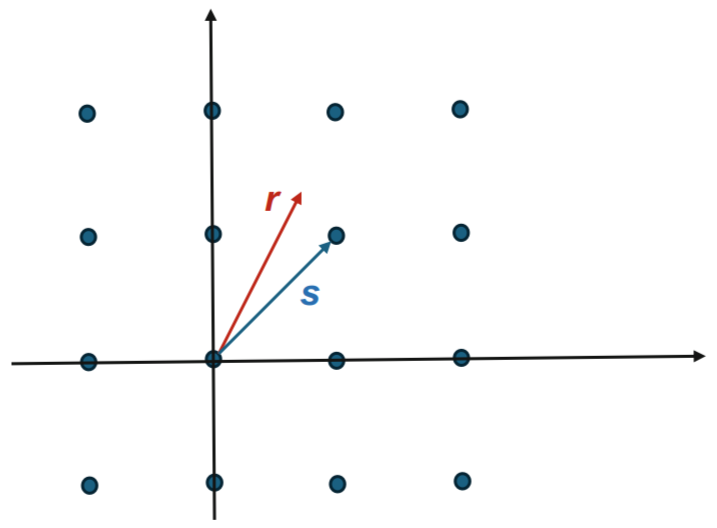
\includegraphics[width=0.8\textwidth]{chapters/figs/fig-12-1}
	\caption{تصویرسازی مسئله کوتاه‌ترین بردار.}
	\label{fig:12-1}
\end{figure}

\subsection{رمزنگاری مبتنی بر یادگیری با خطای ماتی (LWE)}
\label{subsec:12-2-1}
الگوریتم‌های رمزنگاری مبتنی بر مشبکه با برخی از مسائل فهرست‌شده در بالا مرتبط هستند. در رمزنگاری مبتنی بر یادگیری با خطا\LTRfootnote{Learning with errors (LWE)} (\lr{LWE})، ما عناصر بردارهای پایه را به‌صورت تصادفی از $\mathbb{Z}_q^n$ انتخاب می‌کنیم، که در آن $\mathbb{Z}_q$ مجموعه اعداد صحیح در پیمانه $q$ است.






ماتریس $\bm{A}$ و پارامتر $q$ به‌صورت عمومی در دسترس قرار می‌گیرند. یک پروتکل ساده مبتنی بر \lr{LWE}، معروف به یادگیری با خطای ماتی\LTRfootnote{Module learning with errors (module-LWE)} (\lr{module-LWE})، می‌تواند به‌صورت زیر توصیف شود. بردار خصوصی (محرمانه)\LTRfootnote{Private (secret) vector} آلیس، $|s_A\rangle$، از طریق $|p_A\rangle = \bm{A}|s_A\rangle$ با بردار عمومی\LTRfootnote{Public vector} $|p_A\rangle$ در ارتباط است. تولید ماتریس $\bm{A}$ و بردار عمومی آلیس $|p_A\rangle$ نشان‌دهنده گام تولید کلید است. باب بردار خصوصی $\langle s_B|$ و بردار خطا\LTRfootnote{Error vector} $\langle e|$ را تولید کرده و از آن‌ها برای تولید بردار خام عمومی $\langle p_B|$ و اسکالر\LTRfootnote{Scalar} $c$، که بخشی از رمزنگاشت\LTRfootnote{Ciphertext} است، به‌صورت زیر استفاده می‌کند: $\langle p_B| = \langle s_B|\bm{A} + \langle e|$ و $c = \langle s_B|p_A\rangle + e + bq/2$، که در آن $b \in \{0,1\}$ بیتی است که باید رمزگذاری شود. مؤلفه‌های خطا $e_i$ ($i = 1, \dots, m$) و $e$ به‌صورت تصادفی انتخاب می‌شوند اما باید بسیار کوچک‌تر از $q/4$ باشند. بنابراین، باب گام رمزگذاری را برای به‌دست آوردن رمزنگاشتِ متشکل از $\langle p_B|$ و $c$ انجام می‌دهد. آلیس با به‌کارگیری بردار خصوصی خود $|s_A\rangle$ عمل رمزگشایی را به‌صورت زیر انجام می‌دهد:
\begin{equation}
	\begin{aligned}
		b' &= \frac{2}{q} (c - \langle p_B|s_A\rangle) = \frac{2}{q} \left[ \underbrace{\langle s_B|\bm{A}|s_A\rangle}_{|p_A\rangle} + e + bq/2 - (\langle s_B|\bm{A} + \langle e|) |s_A\rangle \right] \\
		&= \frac{2}{q} [\langle s_B|\bm{A}|s_A\rangle + e + bq/2 - \langle s_B|\bm{A}|s_A\rangle - \langle e|s_A\rangle] \\
		&= b + \frac{2}{q} (e - \langle e|s_A\rangle).
	\end{aligned}
	\label{eq:12-2}
\end{equation}
با توجه به اینکه مقدار $\frac{2}{q}(e - \langle e|s_A\rangle)$ عدد کوچکی است و مانند نویز عمل می‌کند، بیت رمزگشایی‌شده $b'$ با بیت باب یعنی $b$ برابر خواهد بود.

همچنین می‌توان تفسیر زیر را ارائه داد \cite{12-22}. در گام تولید کلید، آلیس فهرست-$\bm{A}$ را به‌صورت برداری با طول $n$ از اعداد تصادفی در پیمانه $q$ تولید می‌کند که اعضای آن $A_i \in \mathbb{Z}_q$ هستند. او همچنین یک الگوی خطا به طول $n$ با مؤلفه‌هایی تولید می‌کند که آن‌ها نیز از $\mathbb{Z}_q$ اما کوچک‌تر از $q/n$ هستند. او سپس فهرست-$\bm{B}$ را به‌صورت زیر ایجاد می‌کند:
\begin{equation}
	B_i = A_i s + e_i \pmod q,
	\label{eq:12-3}
\end{equation}
که در آن $s$ عدد محرمانه است. او فهرست‌های $\bm{A}$ و $\bm{B}$ را به‌عنوان کلید عمومی منتشر می‌کند. باب با نمونه‌برداری و انتخاب $K$ نمونه از فهرست-$\bm{B}$، بیت $b$ را به‌صورت زیر رمزگذاری می‌کند:
\begin{equation}
	v = \sum_{j \in \text{Positions}} B_j - bq/2 \mod q,
	\label{eq:12-4}
\end{equation}

که در آن مجموعه \textit{مکان‌ها}\LTRfootnote{Positions} نشان‌دهنده محل نمونه‌ها است. برای رمزگشایی، آلیس ابتدا عدد $u$ را از طریق رابطه زیر ایجاد می‌کند:
\begin{equation}
	u = \sum_{j \in \text{Positions}} A_j \mod q,
	\label{eq:12-3}
\end{equation}

و بیت باب را با استفاده از رابطه زیر و از طریق گرد کردن\LTRfootnote{Rounding} رمزگشایی می‌کند:
\begin{equation}
	b' = \frac{2}{q}\left(v - su \mod q\right),
	\label{eq:12-5}
\end{equation}















	\bibliographystyle{plainnat-fa}
	\bibliography{ref}


	
\end{document}